\documentclass[UTF8,11pt,openany]{ctexbook}
\usepackage[a4paper,margin=26mm]{geometry}
\usepackage{amsmath,amssymb,amsthm,graphicx,enumitem,hyperref}
\hypersetup{unicode=true,colorlinks=true,linkcolor=blue}
\newcommand{\R}{\mathbb{R}}
\newcommand{\Z}{\mathbb{Z}}
\DeclareMathOperator{\Bd}{Bd}
\DeclareMathOperator{\Int}{Int}
\newcommand{\sourcepage}[1]{\par\smallskip{\footnotesize\textit{〔原书第 #1 页〕}}\par\smallskip}
\newcommand{\entry}[2]{\par\medskip\noindent\textbf{#1 #2}\quad}
\newcommand{\translatornote}[1]{\footnote{译注：#1}}
\setlist[enumerate]{itemsep=3pt,topsep=5pt}
\setlength{\emergencystretch}{3em}
\title{代数拓扑基础\\第二版\\中文译稿}
\author{James R. Munkres\\Steven G. Krantz\\Harold R. Parks}
\date{}
\begin{document}
\frontmatter
\maketitle
\chapter*{译稿说明}
本稿收入原书八章正文、习题、书前资料及书末资料。章节、定理编号和原书页码提示保留；索引中的数字指原书页码。插图沿用原图，图内文字保留。原书明显排印错误在必要处以译注说明。本稿尚未经逐页视觉校对，已知图片裁剪问题按读者约定留待反馈后处理。
\chapter*{书籍介绍与作者简介}
\addcontentsline{toc}{chapter}{书籍介绍与作者简介}
本经典教材时隔四十年首次推出新版。在两位新作者协助下，新版为新一代数学工作者和学生更新了内容。

《代数拓扑基础》以具体方式介绍本学科，涵盖同调、上同调、泛系数定理、Künneth 定理、流形对偶，以及经典点集拓扑定理的应用，适合向初学者讲解复杂概念和代数拓扑的趣味。

第二版保留原版特色，多数记号和术语不变，同时增添同伦理论导引、符号索引和许多新习题。代数拓扑是现代数学的基石，每位数学工作者都应有所了解。本书主要依靠三角剖分理论展开，适合学生及资深数学工作者等广泛读者；需要具备一些一般拓扑基础。

James R. Munkres 于 1960—2000 年任教于麻省理工学院数学系，之后继续担任高级讲师。1956 年在 Edwin Moise 指导下获密歇根大学数学博士学位，研究方向为微分拓扑，也是 Munkres 指派算法的提出者，著有多部教材。曾获 1984 年麻省理工学院理学院本科教学奖，1989 年获 Nebraska Wesleyan University 荣誉博士学位。

Steven G. Krantz 在圣路易斯华盛顿大学教授数学，博士毕业于普林斯顿大学，曾任教于加州大学洛杉矶分校、普林斯顿大学及宾夕法尼亚州立大学。已发表 175 余篇学术论文和 65 余部著作，是《几何分析杂志》的创刊编辑、美国数学学会会士，曾获 Chauvenet 奖、Beckenbach 图书奖及 Kemper 奖。

Harold R. Parks 在普林斯顿大学获得数学博士学位，曾任布朗大学 J. D. Tamarkin 讲师，之后到俄勒冈州立大学任教，1989 年晋升教授。1982—1983 学年曾任印第安纳大学访问副教授。在俄勒冈州立大学数学系先后担任系主任助理、副系主任和系主任。著有 8 部书、42 篇学术论文，担任两份期刊的编辑，并为美国数学学会会士。

\chapter*{丛书信息}
\addcontentsline{toc}{chapter}{丛书信息}
\textbf{数学教材丛书（Textbooks in Mathematics）}\par
丛书主编：Al Boggess、Kenneth H. Rosen。
\begin{description}[style=nextline]
\item[《业务流程分析：建模、仿真与设计》] Manuel Laguna、Johan Marklund。
\item[《通过游戏与博彩学习数量素养》] Mark Hunacek。
\item[《测度与积分：理论与实践》] John Srdjan Petrovic。
\item[《现代抽象代数》第十一版] Joseph A. Gallian。
\item[《Gallian〈现代抽象代数〉学生习题解答手册》第十一版] Joseph A. Gallian。
\item[《代数：群、环与域》第二版] Louis Halle Rowen、Uzi Vishne。
\item[《应用数学工作者的泛函分析》] Todd Arbogast、Jerry L. Bona。
\item[《探索线性代数：Mathematica 实验与项目》第二版] Crista Arangala。
\item[《测度论与函数的精细性质》第二版] Lawrence Craig Evans、Ronald R. Gariepy。
\item[《集合论：公理推理导引》] Robert André。
\item[《通过建模介绍微分方程与差分方程》] William P. Fox、Robert E. Burks。
\item[《抽象代数：交互式方法》第三版] William Paulsen。
\item[《代数拓扑基础》第二版] James R. Munkres、Steven G. Krantz、Harold R. Parks。
\end{description}
丛书页面：\url{https://www.routledge.com/Textbooks-in-Mathematics/book-series/CANDHTEXBOOMTH}。

\chapter*{原书版本与版权信息}
\addcontentsline{toc}{chapter}{原书版本与版权信息}
\textbf{Elements of Algebraic Topology，Second Edition}\par
作者：James R. Munkres、Steven G. Krantz、Harold R. Parks。

封面图像由 Carlos Sequin 提供，保留所有权利。第二版于 2025 年由 CRC Press 出版。出版地址：2385 Executive Center Drive, Suite 320, Boca Raton, FL 33431, U.S.A.；以及 4 Park Square, Milton Park, Abingdon, Oxon, OX14 4RN。CRC Press 是 Taylor \& Francis Group, LLC 旗下品牌。

版权 © 2025 James R. Munkres、Steven G. Krantz、Harold R. Parks。第一版由 CRC Press 于 1993 年出版。

作者和出版方已尽合理努力确保资料可靠，但不对全部材料的有效性及使用后果承担责任。已尽力查找所转载材料的版权所有者；若有未获许可或未注明来源之处，请联系出版方，以便在今后重印时修正。

除美国版权法允许的情形外，未经出版方书面许可，本书任何部分不得以现有或未来的电子、机械或其他方式重印、复制、传播或使用，包括复印、缩微、录音及信息存储或检索系统。

复印或电子使用许可可通过 \url{https://www.copyright.com} 申请，或联系 Copyright Clearance Center, Inc.，222 Rosewood Drive, Danvers, MA 01923，电话 978-750-8400。不在其服务范围的作品，请联系 \nolinkurl{mpkbookspermissions@tandf.co.uk}。

商标说明：产品或公司名称可能为商标或注册商标，使用仅为识别与说明，无侵权意图。

美国国会图书馆出版编目资料：\par
ISBN 978-1-032-76554-9（精装）；978-1-041-02924-3（平装）；978-1-003-62147-8（电子书）。\par
DOI：10.1201/9781003621478。

原书采用 CMR10 字体，由 KnowledgeWorks Global Ltd. 排版。出版方说明：本书依据作者提供的可直接制版稿制作。

\chapter*{献词}
\addcontentsline{toc}{chapter}{献词}
献给 Barbara。

谨以此书纪念教我拓扑学的 Marvin J. Greenberg。

献给 Susan。

\tableofcontents
\IfFileExists{sections/frontmatter.tex}{\chapter*{前言}
\addcontentsline{toc}{chapter}{前言}
\sourcepage{xi--xii}
代数拓扑是现代数学的基石之一。每一位从事数学工作的人都应当至少对这门学科有所了解。James R. Munkres 的《代数拓扑基础》是一部提供这种入门介绍的经典著作。如今，这本书问世已有四十年，需要加以更新。本次新版正是为了实现这一目的。

当然，我们保留了原书的基本特色。大部分记号和术语保持不变，第一版的所有核心主题也都予以保留。不过，新版作出了一些有益的增补和修改。

与第一版不同，我们在讨论基本群的一节中介绍了同伦论。无环模型一节经过全面重写，以便读者更容易理解。书末集中收录了正文中提到的各位人物的一些简短生平资料。此外，还列出了一份简短的补充阅读书目，其中大多数书籍出版于第一版之后。另一项新增内容是十分详尽的符号索引；全书的主题索引现在也更加详尽。最后，我们增加了相当数量的习题，其中多数属于巩固练习。

\section*{本书的组织结构}
前两章以单纯同调为基础；在各种同调理论中，它最为具体，因此学生应当比较容易掌握。第三章介绍更抽象的内容，包括 Eilenberg--Steenrod 公理。第四章介绍奇异同调论及其许多有趣的应用，并把 CW 复形作为计算工具引入。对于一学期的课程，前四章是合适的内容。

标有星号的各节，在这一学期课程中可以作为选学内容。当然，在作者看来，那些应用十分有趣，因此即使属于选学内容，教师仍可能选择讲授其中一部分或全部。

第五章介绍上同调论，并最终讨论上同调环。第六章引入张量积，并进一步讨论第一章某个选学小节中提到的任意系数同调。虽然前六章的内容很可能超出一学期课程的容量，但它们构成了扎实的核心内容，应当适合相当广泛的数学工作者，包括学生和资深数学家。

对于两学期的课程，整本书都可以作为教学内容。当然，教师在设计合适的课程时需要有所取舍。对一学期课程而言属于选学的各节，例如“范畴与函子”，对于两学期课程可能是必要的。最后两章彼此独立，因此，如果第二学期接近结束时必须删减一些内容，也可以灵活处理。

具体来说，第七章讨论同调代数，包括各种情形下的泛系数定理和 Künneth 定理。第八章讨论流形，特别是与 Poincaré、Lefschetz、Alexander 和 Pontryagin 的名字相联系的各种对偶定理。为研究 Pontryagin 对偶，本章还引入 Čech 上同调。

如果教师希望减少讲授单纯同调所花的时间，可以略去第二章。这样一来，单纯同调群的拓扑不变性就不再直接证明，而必须通过奇异同调群的不变性，以及单纯同调与奇异同调之间的同构来获得。

\section*{预备知识}
我们假定学生对一般拓扑已有一定了解，包括紧致性、连通性和商空间。书中将用到正规空间上的 Tietze 扩张定理，而商空间尤其重要。我们将在适当之处复习商空间。

我们也希望学生具有一定的代数知识，特别是熟悉群、商群和同态，以及环、域和向量空间。书中不需要用到特别深入的定理。与商空间一样，我们将在适当之处复习基本的代数结果。

\chapter*{致谢}
\addcontentsline{toc}{chapter}{致谢}
\sourcepage{xiii}
我们感谢加利福尼亚大学伯克利分校的 Carlo H. Séquin 提供封面插图。该图展示了两个 Möbius 带如何拼合成一个 Klein 瓶。

感谢编辑 Robert Ross 给予我们的支持与鼓励。我们期待收到读者的反馈。

\begin{flushright}
Steven G. Krantz\\Harold R. Parks
\end{flushright}
}{}
\mainmatter
\chapter{单纯复形的同调群}
\IfFileExists{sections/1-01.tex}{\section{引言}
\sourcepage{1--2}
拓扑学的一个基本问题是：对于给定的两个空间，判定它们是否同胚。要证明两个空间同胚，需要构造从一个空间到另一个空间的连续双射，并且其逆映射也连续。要证明两个空间不同胚，则必须证明这样的映射不存在。这通常更为困难。常见的方法是找出某种拓扑性质，即在同胚下保持不变的性质，使得一个空间具有这种性质，而另一个空间没有。例如，$\R^2$ 中的闭单位圆盘不可能与平面 $\R^2$ 同胚，因为闭圆盘是紧致的，而平面不是。实直线 $\R$ 也不可能与 $\R^2$ 同胚，因为从 $\R$ 中删去一个点后，剩余空间不连通，而从 $\R^2$ 中删去一个点则不会如此。

在处理同胚问题时，这些初等性质的作用相当有限。例如，要在同胚意义下对所有紧致曲面进行分类，就需要比上述性质更精细的拓扑不变量。一般地，当 $n\ne m$ 时，要证明 $\R^n$ 与 $\R^m$ 不同胚，也需要这样的不变量。

代数拓扑起源于 Henri Poincaré、Enrico Betti 等数学家构造这类拓扑不变量的尝试。Poincaré 引入了一种群，称为拓扑空间的\textbf{基本群}（fundamental group）；根据其定义，它就是一个拓扑不变量。人们可以相当容易地证明，球面、环面、Klein 瓶等一些熟悉空间的基本群彼此不同，因此这些空间不可能同胚［见 [Mun00] 第 60 节］。事实上，可以利用基本群对所有紧致曲面进行分类［见 [Mas91] 第 4 章第 5 节］。

代数学家 Emmy Noether 推动了研究重点从空间的数值不变量转向空间的同调群。这是因为，在 20 世纪 20 年代中期，Paul Alexandroff 和 Heinz Hopf 曾到 Göttingen 访问，当时 Noether 在该校数学系任职。她认识到，Alexandroff 和 Hopf 所讨论的 Betti 数与挠系数，实际上是与阿贝尔群相联系的不变量；具体说来，就是与同调群相联系的不变量。Hopf 在 1928 年推广 Euler--Poincaré 公式的论文 [Hop28] 的引言中，明确肯定了 Noether 的影响。早期，同调群带来的一个困难在于：它们并非显然是拓扑不变量。一旦证明了这一点，就可以利用这些群来处理同胚问题。

我们将从研究\textbf{同调群}（homology group）开始讨论代数拓扑。随后讨论其他拓扑不变量，例如上同调群和上同调环。我们还将简要介绍同伦群。

定义同调群有几种不同的方法，对于足够良好的空间，这些方法给出相同的结果。我们将详细讨论其中两种：单纯同调群和奇异同调群。首先讨论历史上最先出现的\textbf{单纯同调群}（simplicial homology group）。无论在概念上还是在计算上，它们都很具体、直观。然而，它们只对特别良好的空间，也就是多面体，才有定义；而且，证明它们的拓扑不变性需要付出相当的努力。之后，我们将讨论\textbf{奇异同调群}（singular homology group），它们是作为单纯同调群的推广而引入的。奇异同调群对任意空间都有定义，并且从定义就能直接看出它们是拓扑不变量。此外，在理论研究中，它们比单纯同调群方便得多。虽然奇异同调群不如单纯同调群容易计算，但在两者都有定义时，它们是一致的。

对任意空间定义同调群的第三种方法出自 Eduard Čech。Čech 同调论仍不完全令人满意，但 Čech 上同调论既重要又有用；我们将在本书接近结尾时讨论它。
}{}
\section{单形}
\sourcepage{2--3}
在定义单纯同调群之前，必须先讨论它们所适用的空间类，即所有多面体构成的空间类。\textbf{多面体}（polyhedron）是以线段、三角形、四面体及其高维类似物为基本构件，沿着这些构件的面粘合而成的空间。本节讨论这些基本构件；下一节将用它们构造多面体。

首先，需要研究一点欧氏空间的解析几何。用 $\R^N$ 表示 $N$ 维欧氏空间，以 $0$ 表示欧氏空间的原点。对于 $x=(x_1,x_2,\ldots,x_N)\in\R^N$，$x$ 的\textbf{范数}定义为
\[
\|x\|=\left[\sum_{i=1}^N(x_i)^2\right]^{1/2}.
\]
给定 $\R^N$ 中的点集 $\{a_0,a_1,\ldots,a_n\}$，如果对任意实数 $t_i$，等式
\[
\sum_{i=0}^n t_i=0,\qquad \sum_{i=0}^n t_i a_i=0
\]
都蕴含 $t_0=t_1=\cdots=t_n=0$，就称这个点集是\textbf{几何独立的}（geometrically independent）。

显然，单点集总是几何独立的。简单的代数运算表明，一般地，$\{a_0,a_1,\ldots,a_n\}$ 几何独立，当且仅当向量
\[
a_1-a_0,\ a_2-a_0,\ \ldots,\ a_n-a_0
\]
在线性代数的意义下线性无关。因此，$\R^N$ 中两个不同的点构成几何独立集；三个不共线的点、四个不共面的点等也同样如此。

给定几何独立点集 $\{a_0,a_1,\ldots,a_n\}$，定义这些点\textbf{张成的 $n$ 维平面} $P$ 为满足下式的所有点 $x\in\R^N$ 构成的集合：存在标量 $t_i$，使得
\[
x=\sum_{i=0}^n t_i a_i,\qquad \sum_{i=0}^n t_i=1.
\]
由于各 $a_i$ 几何独立，各 $t_i$ 由 $x$ 唯一确定。注意，每个点 $a_i$ 本身都属于平面 $P$。

平面 $P$ 也可描述为所有满足下式的点 $x$ 构成的集合：存在标量 $t_1,\ldots,t_n$，使得
\[
x=a_0+\sum_{i=1}^n t_i(a_i-a_0).
\]
采用这种形式时，我们称 $P$ 为“过 $a_0$ 且平行于向量 $a_i-a_0$ 的平面”。

容易验证，如果 $\{a_0,a_1,\ldots,a_n\}$ 几何独立，并且 $w$ 位于这些点张成的平面之外，那么 $\{w,a_0,a_1,\ldots,a_n\}$ 几何独立。

$\R^N$ 的\textbf{仿射变换}（affine transformation）$T$ 是由平移与非奇异线性变换复合而成的映射；这里，平移是指对某个固定的 $p$，具有形式 $T(x)=x+p$ 的映射。从定义立即可知，仿射变换保持点集的几何独立性，而且把 $\{a_0,\ldots,a_n\}$ 张成的平面 $P$ 映到 $\{T(a_0),\ldots,T(a_n)\}$ 张成的平面上。

现在，平移 $T(x)=x-a_0$ 把 $P$ 映到 $\R^N$ 中以 $a_1-a_0,\ldots,a_n-a_0$ 为基的向量子空间上。在 $T$ 之后，再复合一个把这些向量映为 $\R^N$ 中前 $n$ 个单位基向量 $\epsilon_1,\ldots,\epsilon_n$ 的线性变换，就得到 $\R^N$ 的一个仿射变换 $S$，使得 $S(a_0)=0$，并且当 $i>0$ 时，$S(a_i)=\epsilon_i$。\translatornote{原文此处写作 $S(s_0)=0$，其中 $s_0$ 未定义；据上下文应为 $a_0$。}映射 $S$ 把 $P$ 映到 $\R^N$ 中由前 $n$ 个坐标确定的平面 $\R^n\times0$ 上。由此便清楚，为什么称 $P$ 为 $\R^N$ 中的“$n$ 维平面”。

\sourcepage{4}
\entry{定义}{1.2.1}设 $\{a_0,a_1,\ldots,a_n\}$ 是 $\R^N$ 中的几何独立集。定义由 $a_0,a_1,\ldots,a_n$ 张成的 \textbf{$n$ 维单形}（$n$-simplex）$\sigma$ 为满足下式的所有点 $x\in\R^N$ 构成的集合：
\[
x=\sum_{i=0}^n t_i a_i,\qquad
\sum_{i=0}^n t_i=1,\quad t_i\geq0\ \text{对所有 }i.\tag{$*$}
\]
各数 $t_i$ 由 $x$ 和条件 $(*)$ 唯一确定，称为点 $x$ 关于 $a_0,a_1,\ldots,a_n$ 的\textbf{重心坐标}（barycentric coordinates）。

\entry{例}{1.2.2}在低维情形，很容易画出单形。当然，$0$ 维单形就是一个点。由 $a_0$ 和 $a_1$ 张成的 $1$ 维单形由所有形如
\[
x=ta_0+(1-t)a_1,\qquad 0\leq t\leq1
\]
的点组成，因此就是连接 $a_0$ 与 $a_1$ 的线段。这个线段可记作 $a_0a_1$。

类似地，由 $a_0,a_1,a_2$ 张成的 $2$ 维单形 $\sigma$ 就是以这三个点为顶点的三角形区域。最容易看出这一点的方法如下。设 $x\ne a_0$，则
\[
x=\sum_{i=0}^2t_i a_i
=t_0a_0+(1-t_0)\bigl[(t_1/\lambda)a_1+(t_2/\lambda)a_2\bigr],
\]
其中 $\lambda=1-t_0$。方括号中的表达式表示连接 $a_1$ 与 $a_2$ 的线段上的一个点 $p$，因为 $(t_1+t_2)/\lambda=1$，且对 $i=1,2$ 有 $t_i/\lambda\geq0$。因此，$x$ 是连接 $a_0$ 与 $p$ 的线段上的一个点，见图 1.2.1。

反过来，可以验证，这样的线段上的每个点都属于 $\sigma$。因此，$\sigma$ 等于连接 $a_0$ 与 $a_1a_2$ 上各点的所有线段的并。也就是说，$\sigma$ 是一个三角形区域，可以记作 $a_0a_1a_2$。
\begin{center}
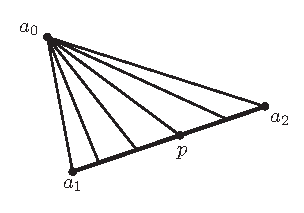
\includegraphics[width=50mm]{figures/1-2-1.pdf}\\图 1.2.1
\end{center}
类似的证明表明，$3$ 维单形就是四面体。

\sourcepage{5}
\entry{定义}{1.2.3}
\begin{enumerate}[label=(\alph*)]
\item 设 $\sigma$ 是由几何独立的点 $a_0,a_1,\ldots,a_n$ 张成的单形。各点 $a_i$ 称为 $\sigma$ 的\textbf{顶点}（vertex），数 $n$ 称为 $\sigma$ 的\textbf{维数}（dimension）。可以把 $\sigma$ 记作 $a_0a_1\cdots a_n$。
\item 由 $\{a_0,a_1,\ldots,a_n\}$ 的某个子集张成的任何单形，称为 $\sigma$ 的一个\textbf{面}（face）。
\item 设 $s$ 是由 $a_0,a_1,\ldots,a_p$ 张成的面，其中 $p<n$；设 $t$ 是由 $a_{p+1},a_{p+2},\ldots,a_n$ 张成的面。称 $t$ 为 $\sigma$ 中与 $s$ \textbf{相对的面}。特别地，由 $a_1,a_2,\ldots,a_n$ 张成的面称为与 $a_0$ 相对的面。
\item $\sigma$ 的不同于其自身的面称为 $\sigma$ 的\textbf{真面}（proper face）。
\item $\sigma$ 的所有真面的并称为 $\sigma$ 的\textbf{边界}（boundary），记作 $\Bd\sigma$。
\item $\sigma$ 的\textbf{内部}（interior）记作 $\Int\sigma$，定义为 $\Int\sigma=\sigma\setminus\Bd\sigma$。务必注意，$0$ 维单形的内部就是该 $0$ 维单形自身；这可能与你的直觉不同。
\item 集合 $\Int\sigma$ 有时称为\textbf{开单形}（open simplex）。
\end{enumerate}
回顾一些标准记号。\textbf{单位 $n$ 维球} $B^n$ 是 $\R^n$ 中满足 $\|x\|\leq1$ 的所有点 $x$ 构成的集合；\textbf{单位球面} $S^{n-1}$ 是满足 $\|x\|=1$ 的点集。$S^{n-1}$ 的\textbf{上半球面} $E_+^{n-1}$ 由其中满足 $x_n\geq0$ 的点组成；\textbf{下半球面} $E_-^{n-1}$ 由其中满足 $x_n\leq0$ 的点组成。

依照这些定义，$B^0$ 是单点空间，$B^1$ 等于区间 $[-1,1]$，$S^0$ 是两点空间 $\{-1,1\}$。二维球是 $\R^2$ 中以原点为中心的单位圆盘，而 $S^1$ 是单位圆周。

\entry{定义}{1.2.4}若对于 $\R^N$ 的子集 $A$ 中任意两点 $x,y$，连接它们的线段都包含在 $A$ 中，则称 $A$ 是\textbf{凸的}（convex）。

还有一个较弱的定义，有时也很有用。

\entry{定义}{1.2.5}若对于 $A\subset\R^N$ 中每个不同于 $w\in A$ 的点 $x$，连接 $x$ 与 $w$ 的线段都包含在 $A$ 中，则称 $A$ \textbf{关于点 $w$ 星形凸}（star-convex）。

下面列出单形的一些基本性质。证明都是初等的，大部分留作习题。

\entry{引理}{1.2.6}设 $P$ 是由几何独立集 $\{a_0,a_1,\ldots,a_n\}$ 确定的 $n$ 维平面，$\sigma$ 是由这些点张成的 $n$ 维单形。
\begin{enumerate}[label=(\arabic*)]
\item 点 $x$ 关于 $a_0,a_1,\ldots,a_n$ 的重心坐标 $t_i(x)$ 是 $x$ 的连续函数。
\item 单形 $\sigma$ 等于连接 $a_0$ 与单形 $s=a_1\cdots a_n$ 中各点的所有线段的并。这样的两条不同线段仅在 $a_0$ 处相交。
\item 单形 $\sigma$ 是 $\R^N$ 中的紧致凸集，并且等于 $\R^N$ 中所有包含 $a_0,a_1,\ldots,a_n$ 的凸集的交。
\item 给定单形 $\sigma$，恰好存在一个张成 $\sigma$ 的几何独立点集。
\item 集合 $\Int\sigma$ 是凸的，在平面 $P$ 中是开集，其闭包为 $\sigma$。此外，$\Int\sigma$ 等于连接 $a_0$ 与 $\Int s$ 中各点的所有开线段的并，其中 $s$ 是 $\sigma$ 中与 $a_0$ 相对的面。
\item 存在从 $\sigma$ 到单位球 $B^n$ 的同胚，它把 $\Bd\sigma$ 映到单位球面 $S^{n-1}$ 上。
\end{enumerate}
\noindent\textbf{证明：}第 (1)--(5) 项留作习题。第 (6) 项是下一个引理的推论；后者是一个更强的结果，在后文也有用。

\sourcepage{6--7}
对于拓扑空间的子集 $A$，我们用 $\overline A$ 表示其闭包，用 $\Int A$ 表示其内部，用 $\Bd A=\overline A\setminus\Int A$ 表示其边界。

\entry{引理}{1.2.7}设 $U$ 是 $\R^n$ 中的有界凸开集，$w\in U$。
\begin{enumerate}[label=(\alph*)]
\item 从 $w$ 出发的每条射线与 $\Bd U=\overline U\setminus U$ 恰好相交于一点。
\item 存在从 $\overline U$ 到 $B^n$ 的同胚，它把 $\Bd U$ 映到 $S^{n-1}$ 上。
\end{enumerate}
\noindent\textbf{证明：}
(a) 给定一条从 $w$ 出发的射线 $R$，其与 $U$ 的交是凸的、有界的，并且在 $R$ 中是开集。因此，这个交由所有形如 $w+tp$ 的点组成，其中 $t$ 遍历某个半开区间 $[0,a)$。所以，点 $x=w+ap$ 是 $R$ 上属于 $\overline U\setminus U$ 的一个点。

假设 $R$ 与 $\overline U\setminus U$ 还相交于另一点 $y$，则对于某个 $b>a$，有 $y=w+bp$。可以写成
\[
x=(1-t)w+ty,\qquad t=a/b.
\]
将其改写为
\[
w=(x-ty)/(1-t).
\]
取 $U$ 中的点列 $y_n$ 收敛于 $y$，并定义
\[
w_n=(x-ty_n)/(1-t).
\]
见图 1.2.2。点列 $w_n$ 收敛于 $w\in U$，所以当某个 $n$ 足够大时，$w_n\in U$。于是，由于 $x=tw_n+(1-t)y_n$，且 $U$ 是凸集，便有 $x\in U$，与 $x$ 的选取矛盾。\translatornote{原文等式为 $x=tw_n+(1-t)y_n$；由上文 $w_n$ 的定义，应为 $x=(1-t)w_n+ty_n$。两系数均在 $(0,1)$ 内，使用正确等式即得所需矛盾。}
\begin{center}
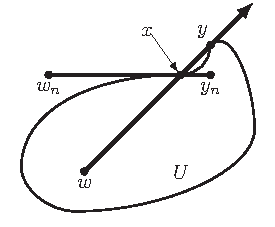
\includegraphics[width=48mm]{figures/1-2-2.pdf}\\图 1.2.2
\end{center}
(b) 为方便起见，设 $w=0$。等式 $f(x)=x/\|x\|$ 定义了从 $\R^n\setminus\{0\}$ 到 $S^{n-1}$ 的连续满射 $f$。由 (a)，$f$ 在 $\Bd U$ 上的限制是到 $S^{n-1}$ 的双射。由于 $\Bd U$ 紧致，这个限制映射是同胚，记其逆映射为 $g$。将 $g$ 扩张成双射 $G:B^n\to\overline U$，使 $G$ 把连接 $0$ 与 $u\in S^{n-1}$ 的线段线性地映到连接 $0$ 与 $g(u)$ 的线段上。具体地，定义
\[
G(x)=\begin{cases}
\|g(x/\|x\|)\|x,&x\ne0,\\
0,&x=0.
\end{cases}
\]
当 $x\ne0$ 时，$G$ 的连续性是显然的。在 $0$ 处的连续性也很容易证明：若 $M$ 是 $\|g(x)\|$ 的一个上界，那么只要 $\|x-0\|<\delta$，就有 $\|G(x)-G(0)\|<M\delta$。\hfill$\square$

\subsection*{习题}
\begin{enumerate}
\item 验证引理 1.2.6 的第 (1)--(3) 项。［提示：若 $T$ 是将 $a_0$ 映为 $0$、将 $a_i$ 映为 $\epsilon_i$ 的仿射变换，那么 $T$ 将点 $x=\sum_{i=0}^n t_i a_i$ 映为点 $(t_1,t_2,\ldots,t_n,0,\ldots,0)$。］
\item 按下列步骤验证引理 1.2.6 的第 (4) 项：
\begin{enumerate}[label=(\alph*)]
\item 证明：如果 $x\in\sigma$ 且 $x\ne a_0,a_1,\ldots,a_n$，那么 $x$ 位于某条包含在 $\sigma$ 中的开线段上。［设 $n>0$。］
\item 证明 $a_0$ 不位于任何包含在 $\sigma$ 中的开线段上。为此证明：若 $a_0=tx+(1-t)y$，其中 $x,y\in\sigma$ 且 $0<t<1$，则 $x=y=a_0$。
\end{enumerate}
\item 验证引理 1.2.6 的第 (5) 项。
\item 如下推广引理 1.2.6 的第 (2) 项。设 $\sigma$ 由 $a_0,a_1,\ldots,a_n$ 张成，$s$ 是由 $a_0,a_1,\ldots,a_p$ 张成的面，其中 $p<n$，而 $t$ 是与 $s$ 相对的面。
\begin{enumerate}[label=(\alph*)]
\item 证明 $\sigma$ 是连接 $s$ 中各点与 $t$ 中各点的所有线段的并，且其中任意两条不同线段至多相交于一个公共端点。
\item 证明 $\Int\sigma$ 是连接 $\Int s$ 中各点与 $\Int t$ 中各点的所有开线段的并。
\end{enumerate}
\item 设 $U$ 是 $\R^n$ 中的有界开集，且 $U$ 关于原点星形凸。
\begin{enumerate}[label=(\alph*)]
\item 证明，从 $0$ 出发的一条射线可能与 $\Bd U$ 相交于多于一个点。
\item[\textasteriskcentered\,(b)] 举例说明，$U$ 不一定与 $B^n$ 同胚。
\end{enumerate}
\end{enumerate}

\section{单纯复形与单纯映射}
\sourcepage{8--9}
\entry{定义}{1.3.1}$\R^N$ 中的\textbf{单纯复形}（simplicial complex）$K$ 是 $\R^N$ 中的一族单形，满足：
\begin{enumerate}[label=(\arabic*)]
\item $K$ 中每个单形的每个面都属于 $K$。
\item $K$ 中任意两个单形的交都是它们各自的一个面。
\end{enumerate}
\entry{例}{1.3.2}图 1.3.1 中的一族单形 $K_1$ 由一个 $2$ 维单形及其各个面组成，是一个单纯复形。$K_2$ 由具有一条公共边的两个 $2$ 维单形及其各个面组成，也是单纯复形；$K_3$ 则不是。那么 $K_4$ 呢？
\begin{center}
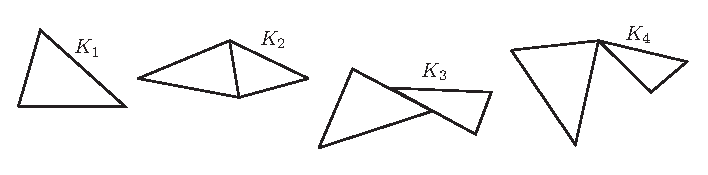
\includegraphics[width=115mm]{figures/1-3-1.pdf}\\图 1.3.1
\end{center}
验证一族单形是否构成单纯复形时，下面的引理有时很有用。

\entry{引理}{1.3.3}一族单形 $K$ 构成单纯复形，当且仅当下列条件成立：
\begin{enumerate}[label=(\arabic*)]
\item $K$ 中每个单形的每个面都属于 $K$。
\item[$(2')$] $K$ 中每一对不同单形的内部不相交。
\end{enumerate}
\noindent\textbf{证明：}先设 $K$ 是单纯复形。给定 $K$ 中两个单形 $\sigma,\tau$，证明：若存在 $x\in\Int\sigma\cap\Int\tau$，则 $\sigma=\tau$。令 $s=\sigma\cap\tau$。如果 $s$ 是 $\sigma$ 的真面，那么 $x$ 就属于 $\Bd\sigma$，这不可能。因此 $s=\sigma$。类似地，$s$ 也不是 $\tau$ 的真面，故 $s=\tau$。由此得到 $\sigma=s=\tau$。

反过来，设 (1) 与 $(2')$ 成立。给定 $K$ 中两个单形 $\sigma,\tau$，假定 $\sigma\cap\tau$ 非空。证明 $\sigma\cap\tau$ 是 $\sigma$ 的一个面 $\sigma'$。具体地，$\sigma'$ 是由 $\sigma$ 的那些属于 $\tau$ 的顶点 $b_0,b_1,\ldots,b_m$ 张成的面。首先，$\sigma'$ 包含在 $\sigma\cap\tau$ 中，因为 $\sigma\cap\tau$ 是包含这些顶点的凸集。为证明反向包含关系，设 $x\in\sigma\cap\tau$。对于 $\sigma$ 的某个面 $s$ 和 $\tau$ 的某个面 $t$，有 $x\in\Int s\cap\Int t$。由 $(2')$ 得 $s=t$。因此 $s$ 的顶点都属于 $\tau$，按定义，它们都属于集合 $\{b_0,\ldots,b_m\}$。所以 $s$ 是 $\sigma'$ 的面，从而得到所需的包含关系。类似地，可以证明 $\sigma\cap\tau$ 是 $\tau$ 的一个面 $\tau'$。这就证明了条件 (2)。\hfill$\square$

由此引理可知，若 $\sigma$ 是单形，则由 $\sigma$ 及其所有真面组成的族是单纯复形：条件 (1) 显然成立；条件 $(2')$ 成立，是因为对于每个点 $x\in\sigma$，恰好存在 $\sigma$ 的一个面 $s$ 使 $x\in\Int s$。

\entry{定义}{1.3.4}若 $L$ 是 $K$ 的一个子族，且包含其各个元素的所有面，则 $L$ 本身也是单纯复形，称为 $K$ 的\textbf{子复形}（subcomplex）。$K$ 的一个子复形是由 $K$ 中维数至多为 $p$ 的所有单形组成的族，称为 $K$ 的 \textbf{$p$ 维骨架}（$p$-skeleton），记作 $K^{(p)}$。族 $K^{(0)}$ 中的点称为 $K$ 的顶点。

\entry{定义}{1.3.5}设 $|K|$ 是 $K$ 的所有单形的并，视为 $\R^N$ 的子集。赋予每个单形作为 $\R^N$ 子空间的自然拓扑，然后如下赋予 $|K|$ 拓扑：规定 $|K|$ 的子集 $A$ 为闭集，当且仅当对每个 $\sigma\in K$，$A\cap\sigma$ 在 $\sigma$ 中是闭集。容易看出这确实定义了一个拓扑，因为这样的集合族对有限并与任意交封闭。空间 $|K|$ 称为 $K$ 的\textbf{底空间}（underlying space），或 $K$ 的\textbf{多胞体}（polytope）。

\sourcepage{10}
作为某个单纯复形的多胞体的空间称为\textbf{多面体}。［注意，有些拓扑学家只把有限单纯复形的多胞体称为多面体。］

一般地，$|K|$ 的这个拓扑比它作为 $\R^N$ 子空间继承的拓扑更细，也就是更大。为说明这一点，注意：若 $A$ 在子空间拓扑下是 $|K|$ 的闭集，则对于 $\R^N$ 的某个闭集 $B$，有 $A=B\cap|K|$。对于 $K$ 中每个单形 $\sigma$，$B\cap\sigma$ 在 $\sigma$ 中闭，因而
\[
A\cap\sigma=B\cap|K|\cap\sigma=B\cap\sigma
\]
在 $\sigma$ 中闭。根据定义，$A$ 在 $|K|$ 的上述拓扑中闭。

一般情况下，$|K|$ 上的子空间拓扑与定义 1.3.5 的拓扑并不相同，见例 1.3.6 和例 1.3.7。不过，若 $K$ 有限，两者就相同。事实上，设 $K$ 有限，且 $A$ 在 $|K|$ 中闭。那么 $A\cap\sigma$ 在 $\sigma$ 中闭，因而在 $\R^N$ 中也闭。由于 $A$ 是有限多个闭集 $A\cap\sigma$ 的并，$A$ 在 $\R^N$ 中也闭。

\entry{例}{1.3.6}设 $K$ 由下列单形及其所有面组成：$\R$ 中所有形如 $[m,m+1]$ 的 $1$ 维单形，其中 $m$ 是非零整数；以及所有形如 $[1/(n+1),1/n]$ 的单形，其中 $n$ 是正整数。那么 $K$ 是一个复形，其底空间作为集合等于 $\R$，但作为拓扑空间则不同。例如，由各点 $1/n$（$n>0$）组成的集合在 $|K|$ 中闭，在 $\R$ 中却不闭。

\entry{例}{1.3.7}设 $K$ 是由 $1$ 维单形 $\sigma_1,\sigma_2,\ldots$ 及其顶点组成的族，其中 $\sigma_i$ 是 $\R^2$ 中以 $0$ 和 $(1,1/i)$ 为顶点的 $1$ 维单形，见图 1.3.2。那么 $K$ 是单纯复形。$|K|$ 与开抛物线弧 $\{(x,x^2):x>0\}$ 的交在 $|K|$ 中是闭集，因为它与每个单形 $\sigma_i$ 的交是单点集。但在 $|K|$ 从 $\R^2$ 继承的拓扑中，它不是闭集，因为在那个拓扑下，原点是它的极限点。
\begin{center}
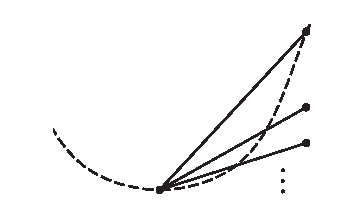
\includegraphics[width=60mm]{figures/1-3-2.pdf}\\图 1.3.2
\end{center}
下面证明多面体的一些初等拓扑性质。

\entry{引理}{1.3.8}若 $L$ 是 $K$ 的子复形，则 $|L|$ 是 $|K|$ 的闭子空间。特别地，若 $\sigma\in K$，则 $\sigma$ 是 $|K|$ 的闭子空间。

\noindent\textbf{证明：}设 $A$ 在 $|L|$ 中闭。若 $\sigma$ 是 $K$ 的一个单形，则 $\sigma\cap|L|$ 是 $\sigma$ 的那些属于 $L$ 的面 $s_i$ 的并。因为 $A$ 在 $|L|$ 中闭，集合 $A\cap s_i$ 在 $s_i$ 中闭，因而在 $\sigma$ 中也闭。由于 $A\cap\sigma$ 是有限多个集合 $A\cap s_i$ 的并，它在 $\sigma$ 中闭。因此 $A$ 在 $|K|$ 中闭。

反过来，若 $B$ 在 $|K|$ 中闭，则对每个 $\sigma\in K$，$B\cap\sigma$ 在 $\sigma$ 中闭，特别是对每个 $\sigma\in L$ 都如此。所以 $B\cap|L|$ 在 $|L|$ 中闭。\hfill$\square$

\sourcepage{11--12}
\entry{引理}{1.3.9}映射 $f:|K|\to X$ 连续，当且仅当对每个 $\sigma\in K$，限制映射 $f|_\sigma$ 连续。

\noindent\textbf{证明：}若 $f$ 连续，则 $f|_\sigma$ 也连续，因为 $\sigma$ 是 $|K|$ 的子空间。反过来，设每个 $f|_\sigma$ 都连续。若 $C$ 是 $X$ 中的闭集，则
\[
f^{-1}(C)\cap\sigma=(f|_\sigma)^{-1}(C),
\]
由 $f|_\sigma$ 的连续性知，这个集合在 $\sigma$ 中闭。因此按定义，$f^{-1}(C)$ 在 $|K|$ 中闭。\translatornote{原文左端印作 $f^{-1}(C\cap\sigma)$；$C$ 与 $\sigma$ 位于不同空间，据上下文应为此处所列等式。}\hfill$\square$

\entry{定义}{1.3.10}设 $X$ 是空间，$\mathcal C$ 是 $X$ 的一族子空间，且其并为 $X$。若 $A$ 在 $X$ 中闭，当且仅当对每个 $C\in\mathcal C$，$A\cap C$ 在 $C$ 中闭，则称 $X$ 的拓扑与族 $\mathcal C$ \textbf{相干}（coherent）。等价地，也可要求：$U$ 在 $X$ 中开，当且仅当对每个 $C\in\mathcal C$，$U\cap C$ 在 $C$ 中开。

特别地，$|K|$ 的拓扑与子空间族 $\{\sigma:\sigma\in K\}$ 相干。

引理 1.3.9 的类似结论对一般的相干拓扑也成立：映射 $f:X\to Y$ 连续，当且仅当对每个 $C\in\mathcal C$，$f|_C$ 连续。

下面把定义 1.2.1 中的重心坐标扩张为定义在多面体上的一族函数。

\entry{定义}{1.3.11}设 $v$ 是单纯复形 $K$ 的任意顶点。如下定义\textbf{重心坐标} $t_v:|K|\to[0,1]$。点 $x\in|K|$ 恰好位于 $K$ 的一个单形的内部，设该单形的顶点为 $a_0,\ldots,a_n$。于是存在正数 $t_0,\ldots,t_n$，使得
\[
x=\sum_{i=0}^n t_i a_i,\qquad \sum_{i=0}^n t_i=1.
\]
若 $v$ 不是其中任何一个顶点 $a_i$，令 $t_v(x)=0$。若 $v$ 是某个顶点，例如 $v=a_{i'}$，则令 $t_v(x)=t_{i'}$。

固定 $v$ 后，函数 $t_v(x)$ 在 $K$ 的每个固定单形 $\sigma$ 上的限制都是连续的，因为它或者在 $\sigma$ 上恒为零，或者等于先前定义的、$x$ 关于 $\sigma$ 的顶点 $v$ 的重心坐标。因此由引理 1.3.9，$t_v(x)$ 在 $|K|$ 上连续。

\entry{引理}{1.3.12}多面体 $|K|$ 是 Hausdorff 空间。

\noindent\textbf{证明：}给定 $|K|$ 中两点 $x_0\ne x_1$，至少存在一个顶点 $v$，使 $t_v(x_0)\ne t_v(x_1)$。在这两个数之间选取 $r$。则集合 $\{x:t_v(x)<r\}$ 与 $\{x:t_v(x)>r\}$ 就是所需的两个不相交开集，分别包含这两个点。\hfill$\square$

\entry{引理}{1.3.13}若 $K$ 有限，则 $|K|$ 紧致。反过来，若 $|K|$ 的子集 $A$ 紧致，则存在 $K$ 的某个有限子复形 $K_0$，使 $A\subset|K_0|$。

\noindent\textbf{证明：}若 $K$ 有限，则 $|K|$ 是有限多个紧致子空间 $\sigma$ 的并，因而紧致。

现设 $A\subset|K|$ 紧致，而且 $A$ 不包含在 $K$ 的任何有限子复形的多胞体中。只要 $A\cap\Int s$ 非空，就从中选取一点 $x_s$。那么集合 $B=\{x_s\}$ 是无限集。此外，$B$ 的每个子集都是闭集，因为它与任何单形 $\sigma$ 的交都是有限集。由于 $B$ 闭且离散，它没有极限点，这与紧致空间的每个无限子集都有极限点这一事实矛盾。\hfill$\square$

研究 $|K|$ 的局部性质时，有三个特定子空间经常有用，现介绍如下。

\entry{定义}{1.3.14}若 $v$ 是 $K$ 的一个顶点，则 $v$ 在 $K$ 中的\textbf{星形邻域}（star），记作 $\operatorname{St}v$，有时也记作 $\operatorname{St}(v,K)$，是 $K$ 中所有以 $v$ 为顶点的单形的内部的并。其闭包记作 $\overline{\operatorname{St}v}$，称为 $v$ 在 $K$ 中的\textbf{闭星形邻域}（closed star）。它是 $K$ 中所有以 $v$ 为顶点的单形的并，也是 $K$ 的某个子复形的多胞体。集合 $\overline{\operatorname{St}v}\setminus\operatorname{St}v$ 称为 $v$ 在 $K$ 中的\textbf{链环}（link），记作 $\operatorname{Lk}v$，见图 1.3.3。
\begin{center}
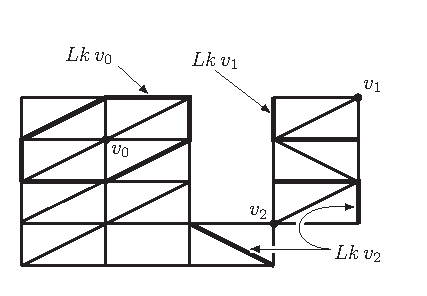
\includegraphics[width=76mm]{figures/1-3-3.pdf}\\图 1.3.3
\end{center}
$\operatorname{St}v$ 在 $|K|$ 中开，因为它恰由满足 $t_v(x)>0$ 的点组成。它的补集是 $K$ 中所有不以 $v$ 为顶点的单形的并，因此是 $K$ 的一个子复形的多胞体。$\operatorname{Lk}v$ 也是 $K$ 的一个子复形的多胞体；它是 $\overline{\operatorname{St}v}$ 与 $\operatorname{St}v$ 的补集的交。容易看出，$\operatorname{St}v$ 和 $\overline{\operatorname{St}v}$ 都道路连通，但 $\operatorname{Lk}v$ 不一定连通。

\sourcepage{13--14}
\entry{定义}{1.3.15}若 $K$ 的每个顶点只属于 $K$ 中有限多个单形，则称单纯复形 $K$ \textbf{局部有限}（locally finite）。换言之，$K$ 局部有限，当且仅当每个闭星形邻域 $\overline{\operatorname{St}v}$ 都是 $K$ 的某个有限子复形的多胞体。

\entry{引理}{1.3.16}复形 $K$ 局部有限，当且仅当空间 $|K|$ 局部紧致。

\noindent\textbf{证明：}设 $K$ 局部有限。给定 $x\in|K|$，它位于 $K$ 的某个顶点 $v$ 的星形邻域 $\operatorname{St}v$ 中。因为 $\overline{\operatorname{St}v}$ 是紧致集，$|K|$ 局部紧致。逆命题留作习题。\hfill$\square$

\subsection*{单纯映射}
现在介绍从一个复形到另一个复形的“单纯映射”的概念。

\entry{引理}{1.3.17}设 $K,L$ 为复形，$f:K^{(0)}\to L^{(0)}$ 为映射。假设只要 $K$ 的顶点 $v_0,v_1,\ldots,v_n$ 张成 $K$ 的一个单形，点 $f(v_0),f(v_1),\ldots,f(v_n)$ 就是 $L$ 的某个单形的顶点。则 $f$ 可以扩张为连续映射 $g:|K|\to|L|$，满足
\[
x=\sum_{i=0}^n t_i v_i\quad\Longrightarrow\quad
g(x)=\sum_{i=0}^n t_i f(v_i).
\]
称 $g$ 为顶点映射 $f$ 诱导的［线性］\textbf{单纯映射}（simplicial map）。

\noindent\textbf{证明：}注意，$L$ 的顶点 $f(v_0),\ldots,f(v_n)$ 虽然不一定互异，但根据假设，它们仍张成 $L$ 的一个单形 $\tau$。把 $g(x)$ 的表达式“合并同类项”之后，系数仍然非负，而且其和仍为 $1$。为说明合并同类项的含义，设 $f(v_0)=f(v_1)$，其余各点 $f(v_2),\ldots,f(v_n)$ 互异。则
\[
g(x)=\sum_{i=0}^n t_i f(v_i)
=(t_0+t_1)f(v_1)+\sum_{i=2}^n t_i f(v_i).
\]
\translatornote{原文末项求和的下限印作 $3$，但紧接着给出的重心坐标包含 $t_2$；这里按合并同类项的含义取 $2$。}
因此，$\tau$ 由 $f(v_1),f(v_2),\ldots,f(v_n)$ 张成，而 $g(x)$ 是 $\tau$ 中重心坐标为 $(t_0+t_1),t_2,\ldots,t_n$ 的点。所以 $g$ 把 $v_0,\ldots,v_n$ 张成的 $n$ 维单形 $\sigma$ 连续地映到顶点集为 $\{f(v_0),\ldots,f(v_n)\}$ 的单形 $\tau$ 中。

$g$ 作为从 $\sigma$ 到 $\tau$ 的映射是连续的，因而作为从 $\sigma$ 到 $|L|$ 的映射也连续。由引理 1.3.9，$g$ 作为从 $|K|$ 到 $|L|$ 的映射连续。\hfill$\square$

从 $K^{(0)}$ 到 $L^{(0)}$ 的顶点映射 $f$ 决定了从 $|K|$ 到 $|L|$ 的扩张 $g$。当然，将 $g$ 限制在顶点集 $K^{(0)}$ 上，就回到原来的映射 $f$。在不致混淆时，有时只用 $g$，或只用 $f$，同时表示这两个映射。

注意，只要 $v_0,v_1,\ldots,v_n$ 张成 $K$ 的一个单形，即使这些点并不互异，$g$ 的公式仍然成立。关键条件是 $t_i$ 非负且其和为 $1$。再一次合并同类项即可看出这一点。

单纯映射 $g:|K|\to|L|$ 与 $h:|L|\to|M|$ 的复合仍为单纯映射。理由如下：设 $\sigma$ 是由 $v_0,\ldots,v_n$ 张成的 $K$ 的单形。根据假设，无论顶点 $g(v_0),\ldots,g(v_n)$ 是否互异，它们都张成 $L$ 的一个单形。同样，无论 $h(g(v_0)),\ldots,h(g(v_n))$ 是否互异，它们也张成 $M$ 的一个单形。对于 $x\in\sigma$，写作 $x=\sum t_i v_i$，其中 $t_i\geq0$、$\sum t_i=1$，利用 $g$ 的公式得
\[
h(g(x))=h\left(\sum_{i=0}^n t_i g(v_i)\right)
=\sum_{i=0}^n t_i h(g(v_i)).
\]
\entry{引理}{1.3.18}设 $f:K^{(0)}\to L^{(0)}$ 是双射，并且 $K$ 的顶点 $v_0,\ldots,v_n$ 张成 $K$ 的一个单形，当且仅当 $f(v_0),\ldots,f(v_n)$ 张成 $L$ 的一个单形。则诱导的单纯映射 $g:|K|\to|L|$ 是同胚。

映射 $g$ 称为 $K$ 到 $L$ 的\textbf{单纯同胚}（simplicial homeomorphism），或\textbf{同构}（isomorphism）。

\noindent\textbf{证明：}$K$ 的每个单形 $\sigma$ 都被 $g$ 映到与它同维的某个单形 $\tau$ 上。只需证明由顶点对应 $f^{-1}$ 诱导的线性映射 $h:\tau\to\sigma$ 是 $g:\sigma\to\tau$ 的逆映射。若 $x=\sum t_i v_i$，则根据定义，$g(x)=\sum t_i f(v_i)$，因此
\[
h[g(x)]=h\left[\sum t_i f(v_i)\right]
=\sum t_i f^{-1}[f(v_i)]=\sum t_i v_i=x.
\]\hfill$\square$

\entry{推论}{1.3.19}以 $\Delta^N$ 表示由一个 $N$ 维单形及其各个面组成的复形。若 $K$ 是有限复形，则对于某个 $N$，$K$ 同构于 $\Delta^N$ 的一个子复形。

\noindent\textbf{证明：}设 $K$ 的顶点为 $v_0,v_1,\ldots,v_N$。在 $\R^N$ 中选取几何独立的点 $a_0,a_1,\ldots,a_N$，令 $\Delta^N$ 由它们张成的 $N$ 维单形及其所有面组成。顶点映射 $f(v_i)=a_i$ 诱导了 $K$ 与 $\Delta^N$ 的某个子复形之间的同构。\hfill$\square$

\subsection*{一般的单纯复形}
要求单纯复形 $K$ 必须位于某个 $\R^N$ 中，会限制 $K$ 的基数和其中单形的维数。现在去掉这些限制。

\sourcepage{15--16}
设 $J$ 为任意指标集，用 $\R^J$ 表示 $\R$ 与自身的 $J$ 重笛卡尔积。$\R^J$ 的元素是从 $J$ 到 $\R$ 的函数，通常用“元组记号”$(x_\alpha)_{\alpha\in J}$ 表示。逐坐标定义通常的加法与标量乘法，乘积 $\R^J$ 自然成为向量空间。

令 $E^J$ 为 $\R^J$ 的如下子集：其中每个点 $(x_\alpha)_{\alpha\in J}$ 除有限多个坐标外，其余坐标都为零。注意，$E^J$ 是 $\R^J$ 的向量子空间。\translatornote{原文此处将环境向量空间写作 $(x_\alpha)_{\alpha\in J}$，据上下文应指 $\R^J$。}设 $\epsilon_\alpha\in E^J$ 是在指标 $\alpha$ 处取值 $1$、在 $J$ 的其他元素处取值 $0$ 的函数，则 $\{\epsilon_\alpha:\alpha\in J\}$ 是 $E^J$ 的一组基；当 $J$ 无限时，它不是 $\R^J$ 的基。

我们称 $E^J$ 为\textbf{广义欧氏空间}（generalized euclidean space），并赋予由度量
\[
|x-y|=\max_{\alpha\in J}|x_\alpha-y_\alpha|
\]
确定的拓扑。

对于 $\R^N$ 中的复形，前面所作的一切都可推广到 $E^J$ 中的复形。空间 $E^J$ 是某些有限维子空间的并，即由基 $\{\epsilon_\alpha:\alpha\in J\}$ 的有限子集张成的各子空间的并。这样的每个子空间都只是某个 $\R^N$ 的副本。$E^J$ 中任意有限点集 $\{a_0,\ldots,a_n\}$ 都位于这样的一个子空间中；若这些点几何独立，则它们张成的单形也位于同一个子空间中。此外，$E^J$ 的度量在每个这样的子空间上给出通常的拓扑。因此，$E^J$ 中任意有限族单形都位于某个 $\R^N$ 的副本中。我们实际所做的，只是允许处理这样的复形：其中所有单形无法整体放入任何一个 $\R^N$ 中。从概念上看，在 $E^J$ 中工作似乎比在 $\R^N$ 中更复杂，但实际上并不造成困难。

请读者验证，我们的结论对于 $E^J$ 中的复形仍然成立。今后我们将自由使用这些结论。

再补充一点：若 $K$ 是 $\R^N$ 中的复形，则其中每个单形的维数至多为 $N$。另一方面，若 $K$ 是 $E^J$ 中的复形，则其中单形的维数不一定有上界。如果 $K$ 中单形的维数存在最大值，就定义此最大值为 $K$ 的\textbf{维数}，记作 $\dim K$；否则，称 $K$ 为无限维的。

\subsection*{习题}
\begin{enumerate}
\item 设 $K$ 为单纯复形，$\sigma\in K$。什么条件下 $\Int\sigma$ 在 $|K|$ 中开？什么条件下 $\sigma$ 在 $|K|$ 中开？
\item 证明，一般地，$\operatorname{St}v$ 和 $\overline{\operatorname{St}v}$ 都道路连通。
\item \begin{enumerate}[label=(\alph*)]
\item 直接证明例 1.3.7 中的多面体不是局部紧致的。
\item 一般地，证明若复形 $K$ 不局部有限，则空间 $|K|$ 不局部紧致。
\end{enumerate}
\item 证明例 1.3.7 中的多面体不可度量化。［提示：证明它不满足第一可数公理。］
\item 若 $g:|K|\to|L|$ 是把 $\sigma$ 的顶点映到 $\tau$ 的顶点上的单纯映射，证明 $g$ 将 $\sigma$ 的某个面同胚地映到 $\tau$ 上。
\item 验证：只要把本节所有八个引理证明中的 $\R^N$ 都换为 $E^J$，这些证明就可原封不动地用于 $E^J$ 中的复形。
\item 设 $K$ 为复形。证明 $|K|$ 可度量化，当且仅当 $K$ 局部有限。［提示：函数 $d(x,y)=\sup_v|t_v(x)-t_v(y)|$ 在 $K$ 的每个有限子复形上都是与其拓扑相容的度量。］
\item 设 $K$ 为复形。证明 $|K|$ 是正规空间。［提示：若 $A$ 在 $|K|$ 中闭，且 $f:A\to[0,1]$ 连续，利用 Tietze 扩张定理，逐步将 $f$ 扩张到 $A\cup|K^{(p)}|$ 上。］
\item 设 $K$ 是 $\R^N$ 中的复形。证明 $|K|$ 是 $\R^N$ 的子空间，当且仅当 $|K|$ 中每个点 $x$ 都位于 $\R^N$ 的某个只与 $K$ 中有限多个单形相交的开集中。将结论推广到 $E^J$。
\item 证明：由 $\R$ 中所有形如 $[1/(n+1),1/n]$（$n$ 为正整数）的单形及其顶点构成的族是一个复形，其多胞体就是 $\R$ 的子空间 $(0,1]$。
\end{enumerate}

\section{抽象单纯复形}
\sourcepage{16--17}
实际处理具体多面体时，通过列出一族单形并取其并来指定多面体 $X$，并不是很方便。这样做很快就会陷入解析几何的细节：要指定所有单形，并确保它们仅在应当相交之处相交，是一件繁琐的事。通过“抽象单纯复形”来指定 $X$ 要容易得多。下面介绍这个概念。

\entry{定义}{1.4.1}\textbf{抽象单纯复形}（abstract simplicial complex）是一族有限非空集合 $\mathcal S$，满足：若 $A\in\mathcal S$，则 $A$ 的每个非空子集也属于 $\mathcal S$。

$\mathcal S$ 的元素 $A$ 称为 $\mathcal S$ 的一个\textbf{单形}，其维数等于其元素个数减 $1$。$A$ 的每个非空子集称为 $A$ 的一个面。$\mathcal S$ 的维数是其中单形维数的最大值；若不存在这样的最大值，则其维数为无限。$\mathcal S$ 的\textbf{顶点集} $V$ 是 $\mathcal S$ 中所有单点元素的并；我们不区分顶点 $v\in V$ 与 $0$ 维单形 $\{v\}\in\mathcal S$。$\mathcal S$ 的一个本身构成复形的子族，称为 $\mathcal S$ 的子复形。

若存在从抽象复形 $\mathcal S$ 的顶点集到抽象复形 $\mathcal T$ 的顶点集的双射 $f$，使得
\[
\{a_0,a_1,\ldots,a_n\}\in\mathcal S
\quad\Longleftrightarrow\quad
\{f(a_0),f(a_1),\ldots,f(a_n)\}\in\mathcal T,
\]
则称 $\mathcal S$ 与 $\mathcal T$ \textbf{同构}。

\entry{定义}{1.4.2}设 $K$ 为单纯复形，$V$ 为其顶点集。令 $\mathcal K$ 为 $V$ 中所有满足以下条件的子集 $\{a_0,a_1,\ldots,a_n\}$ 构成的族：顶点 $a_0,a_1,\ldots,a_n$ 张成 $K$ 的一个单形。族 $\mathcal K$ 称为 $K$ 的\textbf{顶点模式}（vertex scheme）。

族 $\mathcal K$ 是抽象单纯复形的一个特例。事实上，它是关键的例子，下面的定理说明了这一点。

\entry{定理}{1.4.3}
\begin{enumerate}[label=(\alph*)]
\item 每个抽象复形 $\mathcal S$ 都同构于某个单纯复形 $K$ 的顶点模式。
\item 两个单纯复形线性同构，当且仅当它们的顶点模式作为抽象单纯复形同构。
\end{enumerate}
\noindent\textbf{证明：}(b) 立即由引理 1.3.18 得到。为证明 (a)，作如下构造。给定指标集 $J$，令 $\Delta^J$ 为 $E^J$ 中由标准基 $\{\epsilon_\alpha\}_{\alpha\in J}$ 的有限子集张成的所有单形构成的族。容易看出，$\Delta^J$ 是单纯复形。如果 $\sigma,\tau$ 是其中两个单形，则它们的顶点集合在一起仍几何独立，并张成 $\Delta^J$ 的一个单形。若 $J$ 为无限集，则 $\Delta^J$ 是一个无限维单形。\translatornote{此处“无限维单形”沿用原文的称呼；严格地说，$\Delta^J$ 是由所有有限维面构成的复形，而非前面定义中的某个有限维单形。}

现设 $\mathcal S$ 的顶点集为 $V$。选取足够大的指标集 $J$，使存在单射 $f:V\to\{\epsilon_\alpha\}_{\alpha\in J}$，例如可取 $J=V$。如下指定 $\Delta^J$ 的一个子复形 $K$：对于每个［抽象］单形 $\{a_0,\ldots,a_n\}\in\mathcal S$，由 $f(a_0),\ldots,f(a_n)$ 张成的［几何］单形属于 $K$。显然，$K$ 是单纯复形，而且 $\mathcal S$ 同构于 $K$ 的顶点模式；$f$ 就是两个顶点集之间所需的对应。\hfill$\square$

\entry{定义}{1.4.4}若抽象单纯复形 $\mathcal S$ 同构于单纯复形 $K$ 的顶点模式，则称 $K$ 为 $\mathcal S$ 的一个\textbf{几何实现}（geometric realization）。在相差一个线性同构的意义下，几何实现唯一确定。

下面举例说明，如何利用抽象复形指定具体的单纯复形。

\entry{例}{1.4.5}假定要指定一个单纯复形 $K$，使其底空间同胚于圆柱面 $S^1\times I$，其中 $I$ 表示闭单位区间 $[0,1]$。一种方法是画出图 1.4.1，它把 $K$ 指定为由六个 $2$ 维单形及其各个面组成的族。
\begin{center}
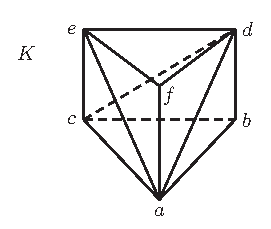
\includegraphics[width=46mm]{figures/1-4-1.pdf}\\图 1.4.1
\end{center}
\sourcepage{18}
表示同一复形 $K$ 的另一种方法是画出图 1.4.2。该图包含两部分：第一，一个底空间为矩形的复形 $L$；第二，对 $L$ 的顶点作出的特定标记，其中某些顶点使用相同的标记。我们把这张图视为如下抽象复形 $\mathcal S$ 的简写：顶点集为字母 $a,b,c,d,e,f$，其单形为
\[
\{a,f,d\},\ \{a,b,d\},\ \{b,c,d\},\ \{c,d,e\},\ \{a,c,e\},\ \{a,e,f\}
\]
以及这些集合的所有非空子集。当然，这个抽象复形同构于先前图中复形 $K$ 的顶点模式，因而在相差线性同构的意义下，它精确指定了同一个复形。也就是说，图 1.4.1 中的 $K$ 是 $\mathcal S$ 的一个几何实现。
\begin{center}
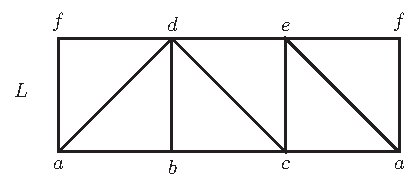
\includegraphics[width=77mm]{figures/1-4-2.pdf}\\图 1.4.2
\end{center}
令 $f:L^{(0)}\to K^{(0)}$ 将 $L$ 的每个顶点映到 $K$ 中具有相同标记的对应顶点。则 $f$ 扩张为单纯映射 $g:|L|\to|K|$。由于这些空间是紧致 Hausdorff 空间，$g$ 是商映射，也就是“粘合映射”。它把 $|L|$ 的右边与左边作线性等同。这正是用一张矩形纸片做成圆柱面的通常方法：把纸片弯过来，将右边粘到左边！

\entry{例}{1.4.6}现在从复形 $L$ 及其顶点的一种标记方式出发。例如，对同一个 $L$ 作另一种顶点标记，如图 1.4.3。与前面一样，这张图指定了某个抽象复形 $\mathcal S$，可以逐一列出其单形。设 $K$ 为 $\mathcal S$ 的几何实现。$K$ 的顶点仍对应于字母 $a,b,\ldots,f$。考虑线性单纯映射 $g:|L|\to|K|$，把 $L$ 的每个顶点映到 $K$ 中具有相同标记的顶点。$g$ 仍是商映射；此时它把 $|L|$ 的左边与右边作线性等同，但要扭转一下。空间 $|K|$ 就是所谓的 \textbf{Möbius 带}。它可以在 $\R^3$ 中画成图 1.4.3 所示的熟悉形状。
\begin{center}
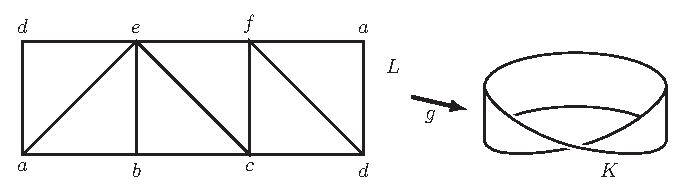
\includegraphics[width=113mm]{figures/1-4-3.pdf}\\图 1.4.3
\end{center}

\sourcepage{19--20}
\entry{例}{1.4.7}\textbf{环面}通常定义为对矩形作图 1.4.4 所示等同而得到的商空间。若要构造底空间同胚于环面的复形，就可以使用图 1.4.5。可以验证，从 $L$ 到此图的几何实现的商映射，恰好完成了构造环面所需要的各项等同。
\begin{center}
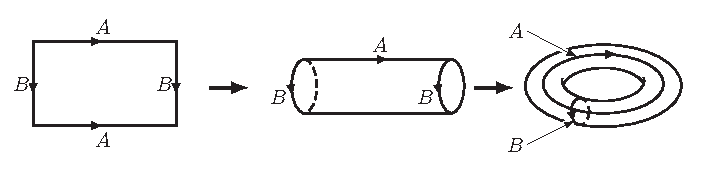
\includegraphics[width=114mm]{figures/1-4-4.pdf}\\图 1.4.4
\medskip

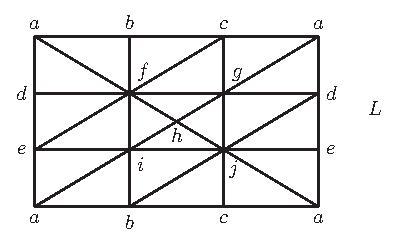
\includegraphics[width=68mm]{figures/1-4-5.pdf}\\图 1.4.5
\end{center}
\entry{例}{1.4.8}一般地，需要小心，确保商映射 $g$ 不会进行超出预期的等同。例如，你可能以为图 1.4.6 确定了环面，其实并非如此。仔细观察该图就会发现，这时的商映射除了把对边粘合，还作了额外的等同。
\begin{center}
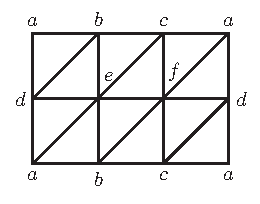
\includegraphics[width=48mm]{figures/1-4-6.pdf}\\图 1.4.6
\end{center}
\entry{例}{1.4.9}图 1.4.7 指定了一个抽象复形，其底空间称为 \textbf{Klein 瓶}。它是将矩形的各边按照图 1.4.8 所示方式粘合得到的商空间。所得空间不能嵌入 $\R^3$，但可以允许它“穿过自身”，从而在 $\R^3$ 中画出示意图。
\begin{center}
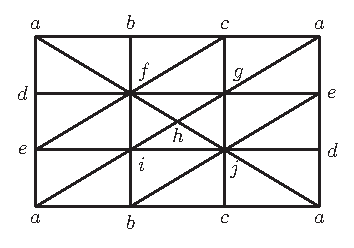
\includegraphics[width=65mm]{figures/1-4-7.pdf}\\图 1.4.7
\medskip

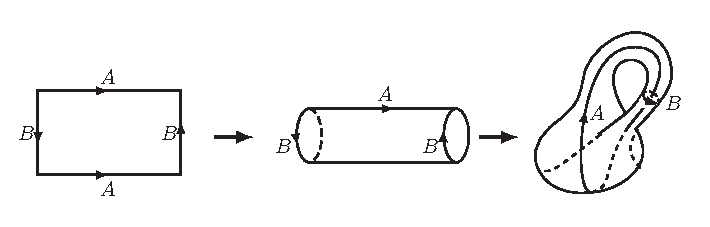
\includegraphics[width=114mm]{figures/1-4-8.pdf}\\图 1.4.8
\end{center}
\entry{例}{1.4.10}\textbf{射影平面} $P^2$ 定义为将二维球面 $S^2$ 中每个点 $x$ 与 $-x$ 等同而得到的空间。习题 2(b) 要求证明：图 1.4.9 确定了一个底空间同胚于 $P^2$ 的复形。\translatornote{原文引用“习题 2(b)”，但本节实际对应的是习题 1(b)。}
\begin{center}
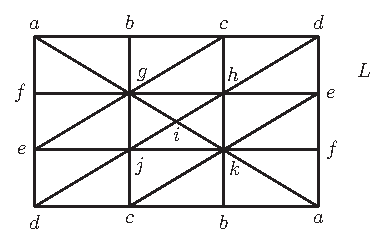
\includegraphics[width=68mm]{figures/1-4-9.pdf}\\图 1.4.9
\end{center}
现在更仔细地说明前面各例所用的过程。给定有限复形 $L$，对其顶点作\textbf{标记}，就是给出从 $L$ 的顶点集到某个集合的满射 $f$，该集合称为\textbf{标记集}。相应的抽象复形 $\mathcal S$ 以这些标记为顶点，其单形为所有形如 $\{f(v_0),\ldots,f(v_n)\}$ 的集合，其中 $v_0,\ldots,v_n$ 张成 $L$ 的一个单形。设 $K$ 为 $\mathcal S$ 的几何实现。由 $f$ 得到的从 $L^{(0)}$ 到 $K^{(0)}$ 的顶点满射扩张为满的单纯映射 $g:|L|\to|K|$。称 $K$ 为\textbf{由带标记复形导出的复形}，称 $g$ 为\textbf{相应的粘合映射}。

由于 $|L|$ 紧致而 $|K|$ 是 Hausdorff 空间，$g$ 把闭集映为闭集，因此 $g$ 是闭商映射。当然，一般地，$g$ 可能把 $L$ 的某个单形映到 $K$ 的一个较低维单形上。例如，$g$ 可能把整个 $L$ 压缩为一个点。我们更关心不会发生这种情况的情形，特别是与前面各例类似的情况。下面的引理给出一般粘合映射 $g$ 具有这些例子中行为的条件。首先需要一个定义。

\sourcepage{21--22}
\entry{定义}{1.4.11}设 $L$ 为复形。如果 $L$ 中每个所有顶点都属于子复形 $L_0$ 的单形，本身也属于 $L_0$，就称 $L_0$ 为 $L$ 的\textbf{满子复形}（full subcomplex）。

例如，图 1.4.5 中矩形 $L$ 的边界是 $L$ 的满子复形，但图 1.4.6 中矩形的边界则不是。

\entry{引理}{1.4.12}设 $L$ 为复形，$f$ 是其顶点的一种标记，$g:|L|\to|K|$ 为相应的粘合映射，$L_0$ 为 $L$ 的满子复形。假设只要 $L$ 的顶点 $v,w$ 具有相同标记，就有：
\begin{enumerate}[label=(\arabic*)]
\item $v,w$ 属于 $L_0$。
\item $\overline{\operatorname{St}v}$ 与 $\overline{\operatorname{St}w}$ 不相交。
\end{enumerate}
则对于所有 $\sigma\in L$，有 $\dim g(\sigma)=\dim\sigma$。此外，若 $g(\sigma_1)=g(\sigma_2)$，则 $\sigma_1,\sigma_2$ 必须是属于 $L_0$ 的不相交单形。\translatornote{此处按原文译出；条件中的顶点应理解为两个不同顶点，结论中的 $\sigma_1,\sigma_2$ 也应理解为两个不同单形，否则取两者相同便不成立。}

证明很容易，留作习题。通常应用这个引理时，$|L|$ 是平面或 $\R^N$ 中的某个多面体区域，$|L_0|$ 是该区域的边界。

\subsection*{习题}
\begin{enumerate}
\item \begin{enumerate}[label=(\alph*)]
\item 证明，$P^2$ 同胚于从 $B^2$ 出发，将每个 $x\in S^1$ 与 $-x$ 等同所得到的空间。
\item 证明图 1.4.9 中的带标记复形 $L$ 确定了一个底空间同胚于 $P^2$ 的复形 $K$。
\item 描述图 1.4.10 中带标记复形所确定的空间。
\end{enumerate}
\begin{center}
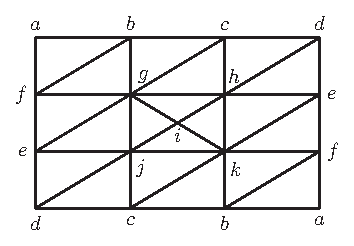
\includegraphics[width=65mm]{figures/1-4-10.pdf}\\图 1.4.10
\end{center}
\item 描述图 1.4.11--1.4.14 中各带标记复形所确定的空间。
\begin{center}
\begin{minipage}{.45\textwidth}\centering
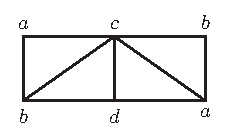
\includegraphics[width=47mm]{figures/1-4-11.pdf}\\图 1.4.11
\end{minipage}\hfill
\begin{minipage}{.45\textwidth}\centering
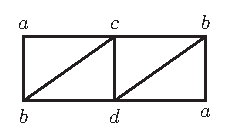
\includegraphics[width=47mm]{figures/1-4-12.pdf}\\图 1.4.12
\end{minipage}
\medskip

\begin{minipage}{.43\textwidth}\centering
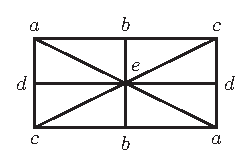
\includegraphics[width=45mm]{figures/1-4-13.pdf}\\图 1.4.13
\end{minipage}\hfill
\begin{minipage}{.53\textwidth}\centering
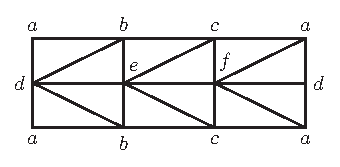
\includegraphics[width=64mm]{figures/1-4-14.pdf}\\图 1.4.14
\end{minipage}
\end{center}
\item 证明引理 1.4.12。
\item 设 $S$ 为带偏序关系 $\leq$ 的集合。组合数学中的一种标准方法是，将抽象复形 $\mathcal S$ 与 $S$ 联系起来：$\mathcal S$ 的顶点是 $S$ 的元素，单形是 $S$ 的有限全序子集。假设 $\{a_1,a_2,\ldots,a_8\}$ 上的偏序由下列关系生成：
\[
\begin{aligned}
a_1&\leq a_3\leq a_7\leq a_8;& a_1&\leq a_5\leq a_7;\\
a_2&\leq a_6\leq a_8;& a_2&\leq a_5.
\end{aligned}
\]
描述 $\mathcal S$ 的一个几何实现。
\end{enumerate}

\section{阿贝尔群回顾}
\sourcepage{23--24}
本节复习后文要用到的一些代数结果，具体来说，是关于阿贝尔群的知识。

对于阿贝尔群，采用加法记号：$0$ 表示单位元，$-g$ 表示 $g$ 的逆元。若 $n$ 是正整数，则 $ng$ 表示 $n$ 项和 $g+g+\cdots+g$，而 $(-n)g$ 表示 $n(-g)$。

用 $\Z$ 表示整数群，$\mathbb Q$ 表示有理数，$\mathbb C$ 表示复数。

\subsection*{同态}
若 $f:G\to H$ 是同态，则 $f$ 的\textbf{核}是 $G$ 的子群 $f^{-1}(0)$，$f$ 的\textbf{像}是 $H$ 的子群 $f(G)$，$f$ 的\textbf{余核}（cokernel）是商群 $H/f(G)$，分别记为 $\ker f$、$\operatorname{im}f$ 和 $\operatorname{cok}f$。映射 $f$ 是单同态，当且仅当它的核只含单位元；通常也形象地说，它的核“消失”。映射 $f$ 是满同态，当且仅当它的余核消失；此时 $f$ 诱导同构 $G/\ker f\cong H$。

\subsection*{自由阿贝尔群}
若阿贝尔群 $G$ 有一组基，就称其为\textbf{自由的}。也就是说，存在一族元素 $\{g_\alpha\}_{\alpha\in J}$，使每个 $g\in G$ 都能唯一写成有限和
\[
g=\sum n_\alpha g_\alpha,
\]
其中每个 $n_\alpha$ 都是整数。唯一性蕴含每个元素 $g_\alpha$ 都具有无限阶，也就是说，$g_\alpha$ 生成 $G$ 的一个无限循环子群。

更一般地，若每个 $g\in G$ 都能写成这样的有限和，但表示不一定唯一，则称族 $\{g_\alpha\}_{\alpha\in J}$ \textbf{生成} $G$。特别地，若该族有限，则称 $G$ \textbf{有限生成}。

若 $G$ 自由，且有一组由 $n$ 个元素 $g_1,\ldots,g_n$ 组成的基，则它的每组基都恰好有 $n$ 个元素。为说明这一点，考察群 $G/2G$ 的元素个数与 $G$ 的基元素个数的关系。给定这组基，$G/2G$ 由所有形如
\[
\sum\epsilon_i g_i+2G,\qquad \epsilon_i=0\ \text{或}\ 1
\]
的陪集组成，因此恰有 $2^n$ 个元素。$G$ 的一组基中元素的个数称为 $G$ 的\textbf{秩}（rank）。

更一般地，若 $G$ 有无限基，那么它的任意两组基具有相同的基数。本书不使用这个事实。

自由阿贝尔群有如下关键性质：若 $G$ 有基 $\{g_\alpha\}_{\alpha\in J}$，则从集合 $\{g_\alpha\}_{\alpha\in J}$ 到阿贝尔群 $H$ 的任意函数 $f$，都能唯一扩张为从 $G$ 到 $H$ 的同态。

构造自由阿贝尔群的一种具体方法如下。给定集合 $S$，定义\textbf{由 $S$ 生成的自由阿贝尔群} $G$ 为所有函数 $\varphi:S\to\Z$ 构成的集合，其中每个函数只在有限多个 $x$ 处非零。通过逐点相加定义两个函数的和。对于 $x\in S$，定义其特征函数
\[
\varphi_x(y)=\begin{cases}0,&y\ne x,\\1,&y=x.\end{cases}
\]
函数族 $\{\varphi_x:x\in S\}$ 构成 $G$ 的一组基，因为每个 $\varphi\in G$ 都能唯一写成有限和 $\sum n_x\varphi_x$，其中 $n_x=\varphi(x)$，对所有使 $\varphi(x)\ne0$ 的 $x$ 求和。我们常滥用记号，将元素 $x\in S$ 与其特征函数 $\varphi_x$ 等同。用此记号，$G$ 的一般元素能唯一写成 $S$ 中元素的有限“形式线性组合” $\sum n_\alpha x_\alpha$。

\sourcepage{25--26}
若存在正整数 $n$ 使 $ng=0$，则称阿贝尔群 $G$ 的元素 $g$ 具有\textbf{有限阶}。$G$ 中所有有限阶元素组成 $G$ 的一个子群 $T$，称为\textbf{挠子群}（torsion subgroup）。若 $T$ 消失，则称 $G$ \textbf{无挠}（torsion-free）。自由阿贝尔群必定无挠，但逆命题不成立。

若 $T$ 只有有限多个元素，则其元素个数称为 $T$ 的\textbf{阶}。若 $T$ 具有有限阶，则其中每个元素都有有限阶，但逆命题仍不成立。

\subsection*{内直和}
设 $G$ 为阿贝尔群，$\{G_\alpha\}_{\alpha\in J}$ 为 $G$ 的一族子群，以某个指标集 $J$ 作一一对应的编号。若 $G$ 中每个元素 $g$ 都能唯一写成有限和 $g=\sum g_\alpha$，其中每个 $g_\alpha\in G_\alpha$，则称 $G$ 是这些群的\textbf{内直和}（internal direct sum），记为
\[
G=\bigoplus_{\alpha\in J}G_\alpha.
\]
若该族有限，例如为 $G_1,\ldots,G_n$，也记为 $G=G_1\oplus\cdots\oplus G_n$。

若 $G$ 中每个 $g$ 都能写成有限和 $g=\sum g_\alpha$，但不一定唯一，则只称 $G$ 为这些群的\textbf{和}，记作 $G=\sum G_\alpha$；有限情形记作 $G=G_1+\cdots+G_n$。此时也称这些子群生成 $G$。

若 $G=\sum G_\alpha$，则此和为直和，当且仅当等式 $0=\sum g_\alpha$ 蕴含对每个 $\alpha$ 都有 $g_\alpha=0$。进而，这只有在对每个固定的指标 $\alpha_0$，都有
\[
G_{\alpha_0}\cap\left(\sum_{\alpha\ne\alpha_0}G_\alpha\right)=\{0\}
\]
时才成立。特别地，若 $G=G_1+G_2$，则此和为直和，当且仅当 $G_1\cap G_2=\{0\}$。

这与自由阿贝尔群非常相似。事实上，若 $G$ 自由且有基 $\{g_\alpha\}$，则 $G$ 是各子群 $G_\alpha$ 的直和，其中 $G_\alpha$ 是由 $g_\alpha$ 生成的无限循环群。反过来，若 $G$ 是无限循环子群的直和，则 $G$ 是自由阿贝尔群。

若 $G$ 是各子群 $G_\alpha$ 的直和，且对于每个 $\alpha$，给定从 $G_\alpha$ 到阿贝尔群 $H$ 的同态 $f_\alpha$，则这些同态能唯一扩张为从 $G$ 到 $H$ 的同态。

下面是证明 $G$ 为直和的一个有用判别准则。

\entry{引理}{1.5.1}设 $G$ 为阿贝尔群。若 $G$ 是各子群 $G_\alpha$ 的直和，则存在同态
\[
j_\beta:G_\beta\to G,\qquad \pi_\beta:G\to G_\beta,
\]
使得当 $\alpha\ne\beta$ 时，$\pi_\beta\circ j_\alpha$ 为零同态；当 $\alpha=\beta$ 时，它为恒等同态。

反过来，设 $\{G_\alpha\}$ 是一族阿贝尔群，且存在上述同态 $j_\beta,\pi_\beta$，则 $j_\beta$ 是单同态。此外，若各群 $j_\alpha(G_\alpha)$ 生成 $G$，则 $G$ 是它们的直和。

\noindent\textbf{证明：}设 $G=\bigoplus_{\alpha\in J}G_\alpha$，定义 $j_\beta$ 为包含同态。为定义 $\pi_\beta$，将 $g$ 写成 $\sum g_\alpha$，其中 $g_\alpha\in G_\alpha$，然后令 $\pi_\beta(g)=g_\beta$。表示的唯一性说明 $\pi_\beta$ 是良定义的同态。

再证逆命题。因为 $\pi_\alpha\circ j_\alpha$ 是 $G_\alpha$ 上的恒等映射，所以 $j_\alpha$ 是单射，$\pi_\alpha$ 是满射。若各群 $j_\alpha(G_\alpha)$ 生成 $G$，则 $G$ 的每个元素都能写成有限和 $\sum j_\alpha(g_\alpha)$。为证明唯一性，设
\[
\sum j_\alpha(g_\alpha)=\sum j_\alpha(g'_\alpha).
\]
在两边作用 $\pi_\beta$，即得 $g_\beta=g'_\beta$。\hfill$\square$

\subsection*{直积与外直和}
设 $\{G_\alpha\}_{\alpha\in J}$ 为一族带指标的阿贝尔群。其\textbf{直积} $\prod_{\alpha\in J}G_\alpha$ 是以各集合 $G_\alpha$ 的笛卡尔积为底集、以逐坐标相加为运算的群。其\textbf{外直和}（external direct sum）$G$ 是直积的如下子群：其中的元组 $(g_\alpha)_{\alpha\in J}$ 除有限多个坐标外，都满足 $g_\alpha=0_\alpha$；这里 $0_\alpha$ 是 $G_\alpha$ 的零元。群 $G$ 有时也称为各群 $G_\alpha$ 的\textbf{弱直积}。

内直和与外直和的关系如下。设 $G$ 为各群 $G_\alpha$ 的外直和。对于每个 $\beta$，定义 $\pi_\beta:G\to G_\beta$ 为到第 $\beta$ 个因子的投影；定义 $j_\beta:G_\beta\to G$，把 $g\in G_\beta$ 映到如下元组：当 $\alpha\ne\beta$ 时，$g_\alpha=0_\alpha$，而 $g_\beta=g$。于是，当 $\alpha\ne\beta$ 时，$\pi_\beta\circ j_\alpha=0$，并且 $\pi_\alpha\circ j_\alpha$ 为恒等映射。因此 $G$ 等于各群 $G'_\alpha=j_\alpha(G_\alpha)$ 的内直和，且 $G'_\alpha\cong G_\alpha$。

\sourcepage{27--28}
所以，内直和与外直和的概念密切相关，主要区别在于记号。因此，通常都用
\[
G=G_1\oplus G_2\oplus\cdots\oplus G_n,\qquad
G=\bigoplus_{\alpha\in J}G_\alpha
\]
表示内直和或外直和，依靠上下文说明含义，如果区分确实重要的话。例如，可以用 $G\cong\Z\oplus\Z\oplus\Z$ 表示 $G$ 是秩为 $3$ 的自由阿贝尔群。

若 $G_1$ 是 $G$ 的子群，且存在 $G$ 的子群 $G_2$ 使 $G=G_1\oplus G_2$，则称 $G_1$ 是 $G$ 的\textbf{直和项}（direct summand）。此时，若 $H_i$ 是 $G_i$ 的子群（$i=1,2$），则和 $H_1+H_2$ 为直和，并且
\[
G/(H_1\oplus H_2)\cong(G_1/H_1)\oplus(G_2/H_2).
\]
特别地，若 $G=G_1\oplus G_2$，则 $G/G_1\cong G_2$。

当然，即使 $G/G_1\cong G_2$，也不一定有 $G=G_1\oplus G_2$；也就是说，$G_1$ 可以是 $G$ 的子群而不是直和项。例如，整数群的子群 $n\Z$ 不是 $\Z$ 的直和项，否则对于 $\Z$ 的某个子群 $G_2$，就有
\[
\Z\cong n\Z\oplus G_2.
\]
于是 $G_2\cong\Z/n\Z$，具有有限阶，而 $\Z$ 没有有限阶子群。\translatornote{该例应取 $n>1$；而且最后一句应理解为 $\Z$ 没有非平凡的有限子群。原文未明说这些限定。}

顺便说明，依照现行用法，模 $n$ 整数群 $\Z/n\Z$ 将简记为 $\Z/n$。

\subsection*{有限生成阿贝尔群基本定理}
实际上，有两个定理对我们很重要。第一个讨论自由阿贝尔群的子群，这里先陈述，在第 1.12 节给出证明。

\entry{定理}{1.5.2}设 $F$ 为自由阿贝尔群，$R$ 为其子群，则 $R$ 也是自由阿贝尔群。若 $F$ 的秩为 $n$，则 $R$ 的秩为 $r\leq n$；此外，存在 $F$ 的一组基 $e_1,\ldots,e_n$ 以及整数 $t_1,\ldots,t_k$（$t_i>1$），使得：
\begin{enumerate}[label=(\arabic*)]
\item $t_1e_1,t_2e_2,\ldots,t_ke_k,e_{k+1},e_{k+2},\ldots,e_r$ 是 $R$ 的一组基。
\item $t_1\mid t_2\mid\cdots\mid t_k$，即每个 $t_i$ 都整除 $t_{i+1}$。
\end{enumerate}
整数 $t_1,\ldots,t_k$ 由 $F$ 和 $R$ 唯一确定，尽管基 $e_1,\ldots,e_n$ 并不唯一。

下面的定理是它的直接推论。

\entry{定理}{1.5.3（有限生成阿贝尔群基本定理）}设 $G$ 为有限生成阿贝尔群，$T$ 为其挠子群。
\begin{enumerate}[label=(\alph*)]
\item $G$ 有一个有限秩 $\beta$ 的自由阿贝尔子群 $H$，使 $G=H\oplus T$。
\item 存在有限循环群 $T_1,\ldots,T_k$，其中 $T_i$ 的阶为 $t_i>1$，使 $t_1\mid t_2\mid\cdots\mid t_k$，并且 $T=T_1\oplus\cdots\oplus T_k$。
\item 数 $\beta$ 及 $t_1,\ldots,t_k$ 由 $G$ 唯一确定。
\end{enumerate}
数 $\beta$ 称为 $G$ 的 \textbf{Betti 数}，各数 $t_1,\ldots,t_k$ 称为 $G$ 的\textbf{挠系数}（torsion coefficients）。注意，$\beta$ 是自由阿贝尔群 $G/T\cong H$ 的秩。子群 $H$ 的秩与各子群 $T_i$ 的阶唯一确定，但这些子群本身不唯一。

\noindent\textbf{证明：}取 $G$ 的有限生成集 $S=\{g_i\}$，设 $F$ 为集合 $S$ 上的自由阿贝尔群。将每个 $g_i$ 映到自身的映射扩张为从 $F$ 到 $G$ 的满同态。记其核为 $R$，则 $F/R\cong G$。按定理 1.5.2 为 $F$ 和 $R$ 选取基，得到
\[
F=F_1\oplus F_2\oplus\cdots\oplus F_n,
\]
其中 $F_i$ 是以 $e_i$ 为生成元的无限循环群，且
\[
R=t_1F_1\oplus\cdots\oplus t_kF_k\oplus F_{k+1}\oplus\cdots\oplus F_r.
\]
于是商群为
\[
F/R\cong(F_1/t_1F_1\oplus\cdots\oplus F_k/t_kF_k)
\oplus(F_{r+1}\oplus\cdots\oplus F_n).
\]
\translatornote{原文商群公式中从第二个因子起，若干分子漏印下标，这里按前述直和分解补齐。}
因此存在同构
\[
f:G\longrightarrow(\Z/t_1\oplus\cdots\oplus\Z/t_k)
\oplus(\Z\oplus\cdots\oplus\Z).
\]
因为同构保持挠子群，$f$ 必须把 $G$ 的挠子群 $T$ 映到 $\Z/t_1\oplus\cdots\oplus\Z/t_k$ 上。由此得到 (a) 和 (b)。第 (c) 项留作习题。\hfill$\square$

\sourcepage{29--30}
这个定理表明，每个有限生成阿贝尔群 $G$ 都能写成有限个循环群的直和，即
\[
G\cong(\Z\oplus\cdots\oplus\Z)\oplus\Z/t_1\oplus\cdots\oplus\Z/t_k,
\]
其中 $t_i>1$ 且 $t_1\mid t_2\mid\cdots\mid t_k$。在某种意义下，这种表示是 $G$ 的一种“典范形式”。还有另一种典范形式，可以如下导出。

先回顾：若正整数 $m,n$ 互素，则 $\Z/m\oplus\Z/n\cong\Z/mn$。因此，任意有限循环群都能写成阶为素数幂的循环群的直和。由定理 1.5.3，对于任意有限生成群 $G$，\translatornote{此处原文写“有限生成群”，按本节语境应理解为“有限生成阿贝尔群”。}有
\[
G\cong(\Z\oplus\cdots\oplus\Z)\oplus\Z/a_1\oplus\cdots\oplus\Z/a_s,
\]
其中每个 $a_i$ 都是某个素数的幂。这也是 $G$ 的一种典范形式，因为正如下面将要看到的，在相差排列的意义下，各数 $a_i$ 由 $G$ 唯一确定。

\subsection*{习题}
\begin{enumerate}
\item 证明：若 $G$ 为有限生成阿贝尔群，则其每个子群都有限生成。［这个结论对非阿贝尔群不成立。］
\item \begin{enumerate}[label=(\alph*)]
\item 证明：若 $G$ 自由，则 $G$ 无挠。
\item 证明：若 $G$ 有限生成且无挠，则 $G$ 自由。
\item 证明有理数加法群 $\mathbb Q$ 无挠但不自由。［提示：若 $\{g_\alpha\}$ 是 $\mathbb Q$ 的一组基，固定 $\beta$，把 $g_\beta/2$ 用这组基表示。］
\end{enumerate}
\item \begin{enumerate}[label=(\alph*)]
\item 证明：若 $m,n$ 互素，则 $\Z/m\oplus\Z/n$ 是阶为 $mn$ 的循环群。
\item 若 $G\cong\Z/18\oplus\Z/36$，将 $G$ 表示为阶为素数幂的循环群的直和。
\item 若 $G\cong\Z/2\oplus\Z/4\oplus\Z/3\oplus\Z/3\oplus\Z/9$，求 $G$ 的挠系数。
\item 若 $G\cong\Z/15\oplus\Z/20\oplus\Z/18$，求 $G$ 的挠系数。
\end{enumerate}
\item \begin{enumerate}[label=(\alph*)]
\item 设 $p$ 为素数，$b_1,\ldots,b_k$ 为非负整数。证明：若
\[
G\cong(\Z/p)^{b_1}\oplus(\Z/p^2)^{b_2}\oplus\cdots\oplus(\Z/p^k)^{b_k},
\]
则各整数 $b_i$ 由 $G$ 唯一确定。［提示：考察同态 $f_i:G\to G$ 的核，其中 $f_i$ 是乘以 $p^i$ 的映射。证明 $f_1,f_2$ 确定 $b_1$，再类似地继续。］
\item 设 $p_1,\ldots,p_N$ 为一列互异素数，将 (a) 推广到形如 $(\Z/(p_i)^k)^{b_{ik}}$（$b_{ik}\geq0$）的项的有限直和。
\item 验证定理 1.5.3 的 (c)，即证明有限生成阿贝尔群 $G$ 的 Betti 数与挠系数由 $G$ 唯一确定。
\item 证明定理 1.5.2 的结论中的各数 $t_i$ 由 $F$ 和 $R$ 唯一确定。
\end{enumerate}
\end{enumerate}

\section{同调群}
\sourcepage{30--31}
现在可以定义同调群了。首先必须讨论“定向”的概念。

\entry{定义}{1.6.1}设 $\sigma$ 为单形，可以是几何单形或抽象单形。若其顶点集的两种排序相差一个偶置换，则定义它们等价。若 $\dim\sigma>0$，则顶点的所有排序分成两个等价类，每个等价类称为 $\sigma$ 的一种\textbf{定向}（orientation）。若 $\sigma$ 为 $0$ 维单形，则只有一个等价类，因而只有一种定向。\textbf{定向单形}（oriented simplex）是单形 $\sigma$ 连同它的一种定向。

若点 $v_0,v_1,\ldots,v_p$ 独立，用符号 $v_0v_1\cdots v_p$ 表示它们张成的单形，用 $[v_0,v_1,\ldots,v_p]$ 表示由该单形连同排序 $(v_0,v_1,\ldots,v_p)$ 的等价类组成的定向单形。

在上下文含义明确时，偶尔也会用单个字母，例如 $\sigma$，表示单形或定向单形。

\entry{例}{1.6.2}我们常用箭头表示 $1$ 维单形的定向。定向单形 $[v_0,v_1]$ 如图 1.6.1 所示，箭头从 $v_0$ 指向 $v_1$。$2$ 维单形的定向用环形箭头表示。图中的定向单形 $[v_0,v_1,v_2]$ 用沿 $v_0$ 到 $v_1$ 再到 $v_2$ 的方向的箭头表示。可以验证，$[v_1,v_2,v_0]$ 与 $[v_2,v_0,v_1]$ 也由同一个顺时针箭头表示。逆时针箭头则表示相反定向的单形。

类似地，定向单形 $[v_0,v_1,v_2,v_3]$ 可用图中的螺旋箭头表示，这个箭头称为“右手螺旋”。如果右手四指沿 $v_0$ 到 $v_1$ 再到 $v_2$ 的方向弯曲，那么拇指指向 $v_3$。可以验证，$[v_0,v_2,v_3,v_1]$，以及与这两种排序等价的另外十种排序，也都给出右手螺旋。“左手螺旋”则表示相反的定向。
\begin{center}
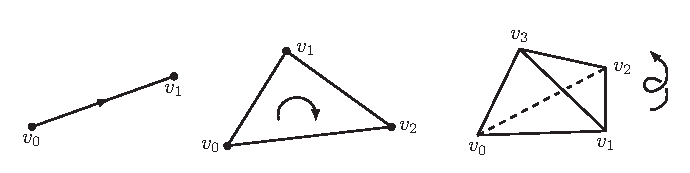
\includegraphics[width=114mm]{figures/1-6-1.pdf}\\图 1.6.1
\end{center}
\entry{定义}{1.6.3}设 $K$ 为单纯复形。$K$ 上的一条 \textbf{$p$ 维链}（$p$-chain），是从 $K$ 的定向 $p$ 维单形集到整数的函数 $c$，满足：
\begin{enumerate}[label=(\arabic*)]
\item 若 $\sigma,\sigma'$ 是同一个单形的相反定向，则 $c(\sigma)=-c(\sigma')$。
\item 除有限多个定向单形外，均有 $c(\sigma)=0$。
\end{enumerate}
通过逐点相加定义 $p$ 维链的加法；所得群记为 $C_p(K)$，称为 $K$ 的\textbf{定向 $p$ 维链群}。若 $p<0$ 或 $p>\dim K$，则令 $C_p(K)$ 为平凡群。

若 $\sigma$ 为定向单形，与它对应的\textbf{初等链}（elementary chain）是如下函数 $c$：
\[
\begin{aligned}
c(\sigma)&=1,\\
c(\sigma')&=-1&&\text{若 $\sigma'$ 是 $\sigma$ 的相反定向},\\
c(\tau)&=0&&\text{对所有其他定向单形 $\tau$}.
\end{aligned}
\]
我们常滥用记号，不仅用 $\sigma$ 表示单形或定向单形，也用它表示相应的初等 $p$ 维链。依此约定，若 $\sigma,\sigma'$ 是同一单形的相反定向，就写作 $\sigma'=-\sigma$，因为把它们解释为初等链时，这个等式成立。

\sourcepage{32--33}
\entry{引理}{1.6.4}群 $C_p(K)$ 是自由阿贝尔群。给每个 $p$ 维单形选择一种定向，相应的初等链就构成 $C_p(K)$ 的一组基。

\noindent\textbf{证明：}证明很直接。任意地给 $K$ 的每个 $p$ 维单形定向，不必参照其他单形的定向。之后，每条 $p$ 维链 $c$ 都能唯一写成相应初等链 $\sigma_i$ 的有限线性组合 $c=\sum n_i\sigma_i$。链 $c$ 在定向单形 $\sigma_i$ 上取值 $n_i$，在其相反定向上取值 $-n_i$，在未出现在此和中的所有定向 $p$ 维单形上取值 $0$。\hfill$\square$

群 $C_0(K)$ 与其他链群不同，它有一组自然的基，因为每个 $0$ 维单形只有一种定向。若 $p>0$，则 $C_p(K)$ 没有“自然”的基，因为必须任意地给各 $p$ 维单形定向，才能得到一组基。

\entry{推论}{1.6.5}从 $K$ 的定向 $p$ 维单形集到阿贝尔群 $G$ 的任意函数 $f$，只要对所有定向 $p$ 维单形满足 $f(-\sigma)=-f(\sigma)$，就能唯一扩张为同态 $C_p(K)\to G$。

\entry{定义}{1.6.6}现在定义称为\textbf{边界算子}（boundary operator）的同态
\[
\partial_p:C_p(K)\longrightarrow C_{p-1}(K).
\]
若 $\sigma=[v_0,v_1,\ldots,v_p]$ 是定向单形，且 $p>0$，定义
\[
\partial_p\sigma=\partial_p[v_0,v_1,\ldots,v_p]
=\sum_{i=0}^p(-1)^i[v_0,v_1,\ldots,\widehat v_i,\ldots,v_p].\tag{$*$}
\]
\translatornote{原文此式的符号印作 $(-1)^p$，而后面的计算和例子均使用 $(-1)^i$；这里采用与后文一致的边界公式。}
其中 $\widehat v_i$ 表示从该序列中删去顶点 $v_i$。由于 $p<0$ 时 $C_p(K)$ 为平凡群，故当 $p\leq0$ 时，$\partial_p$ 为平凡同态。

必须检验 $\partial_p$ 是良定义的。具体地，需要证明 $\partial_p(-\sigma)=-\partial_p(\sigma)$。为此，只需证明：若交换 $[v_0,\ldots,v_p]$ 中两个相邻顶点，$(*)$ 右边就改变符号。比较
\[
\partial_p[v_0,\ldots,v_j,v_{j+1},\ldots,v_p],\qquad
\partial_p[v_0,\ldots,v_{j+1},v_j,\ldots,v_p].
\]
分别展开为四部分，得到
\begin{align*}
\partial_p\sigma={}&\sum_{i<j}(-1)^i[v_0,\ldots,\widehat v_i,\ldots,v_{j-1},v_j,v_{j+1},v_{j+2},\ldots,v_p] &&\text{(a)}\\
&+\sum_{i>j+1}(-1)^i[v_0,\ldots,v_{j-1},v_j,v_{j+1},v_{j+2},\ldots,\widehat v_i,\ldots,v_p] &&\text{(b)}\\
&+(-1)^j[v_0,\ldots,v_{j-1},v_{j+1},v_{j+2},\ldots,v_p] &&\text{(c)}\\
&+(-1)^{j+1}[v_0,\ldots,v_{j-1},v_j,v_{j+2},\ldots,v_p]. &&\text{(d)}
\end{align*}
\begin{align*}
\partial_p(-\sigma)={}&\sum_{i<j}(-1)^i[v_0,\ldots,\widehat v_i,\ldots,v_{j-1},v_{j+1},v_j,v_{j+2},\ldots,v_p] &&\text{(a$'$)}\\
&+\sum_{i>j+1}(-1)^i[v_0,\ldots,v_{j-1},v_{j+1},v_j,v_{j+2},\ldots,\widehat v_i,\ldots,v_p] &&\text{(b$'$)}\\
&+(-1)^j[v_0,\ldots,v_{j-1},v_j,v_{j+2},\ldots,v_p] &&\text{(c$'$)}\\
&+(-1)^{j+1}[v_0,\ldots,v_{j-1},v_{j+1},v_{j+2},\ldots,v_p]. &&\text{(d$'$)}
\end{align*}
(a$'$) 行右边是 (a) 行右边的负值，因为只交换了 $v_j,v_{j+1}$，其他顶点位置不变。同样，(b$'$) 是 (b) 的负值。(c$'$) 是 (d) 的负值，因为顶点顺序相同，而 $-1$ 的指数相差 $1$；同样，(d$'$) 是 (c) 的负值。这就验证了 $\partial_p(-\sigma)=-\partial_p(\sigma)$。

\entry{例}{1.6.7}对于 $1$ 维单形，$\partial_1[v_0,v_1]=v_1-v_0$。对于 $2$ 维单形，
\[
\partial_2[v_0,v_1,v_2]=[v_1,v_2]-[v_0,v_2]+[v_0,v_1].
\]
对于 $3$ 维单形，
\[
\partial_3[v_0,v_1,v_2,v_3]
=[v_1,v_2,v_3]-[v_0,v_2,v_3]+[v_0,v_1,v_3]-[v_0,v_1,v_2].
\]
图 1.6.2 展示了这些公式的几何内容。如果还记得微积分中学过的 Green 定理、Stokes 定理与 Gauss 定理的各种形式，这些图应当相当熟悉。
\begin{center}
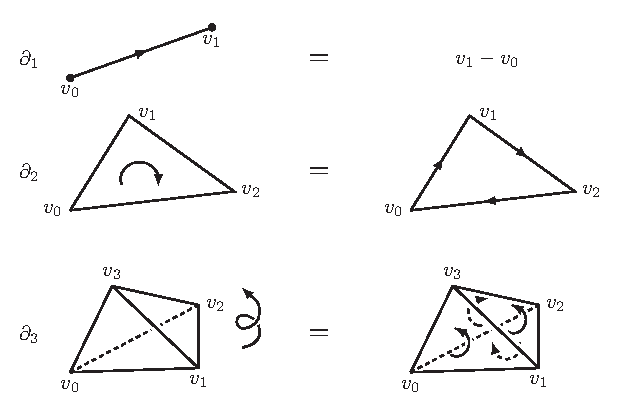
\includegraphics[width=106mm]{figures/1-6-2.pdf}\\图 1.6.2
\end{center}
\entry{例}{1.6.8}考虑图 1.6.2 中的 $1$ 维链 $\partial_2[v_0,v_1,v_2]$。对它作用算子 $\partial_1$，结果为零：每个顶点既是某条边的起点，又是另一条边的终点，因此所有项都抵消了。可以验证，计算 $\partial_2\partial_3[v_0,v_1,v_2,v_3]$ 时也发生类似的抵消。

\sourcepage{34--35}
例 1.6.8 的计算说明了下面的一般事实。

\entry{引理}{1.6.9}对于每个整数 $p$，都有 $\partial_{p-1}\circ\partial_p=0$。

\noindent\textbf{证明：}设 $0<p\leq\dim K$，否则结论平凡。设 $[v_0,\ldots,v_p]$ 为 $K$ 的定向单形，计算得
\begin{align*}
\partial_{p-1}\partial_p[v_0,\ldots,v_p]
&=\partial_{p-1}\left(\sum_{i=0}^p(-1)^i[v_0,\ldots,\widehat v_i,\ldots,v_p]\right)\\
&=\sum_{i=0}^p(-1)^i\partial_{p-1}[v_0,\ldots,\widehat v_i,\ldots,v_p]\\
&=\sum_{i=0}^p\sum_{j<i}(-1)^i(-1)^j[v_0,\ldots,\widehat v_j,\ldots,\widehat v_i,\ldots,v_p]\\
&\quad+\sum_{i=0}^p\sum_{j>i}(-1)^i(-1)^{j-1}[v_0,\ldots,\widehat v_i,\ldots,\widehat v_j,\ldots,v_p].
\end{align*}
这两个和中的各项两两抵消。\hfill$\square$

\entry{定义}{1.6.10}同态 $\partial_p:C_p(K)\to C_{p-1}(K)$ 的核称为 \textbf{$p$ 维闭链群}（group of $p$-cycles），记作 $Z_p(K)$。［字母 Z 来自德语 Zyklus；字母 C 已被用于链。］同态 $\partial_{p+1}:C_{p+1}(K)\to C_p(K)$ 的像称为 \textbf{$p$ 维边界链群}（group of $p$-boundaries），记作 $B_p(K)$。由前一引理，$(p+1)$ 维链的边界自动是 $p$ 维闭链，即 $B_p(K)\subset Z_p(K)$。定义
\[
H_p(K)=Z_p(K)/B_p(K),
\]
称此商群为 $K$ 的\textbf{第 $p$ 同调群}。

下面计算几个例子。

\entry{例}{1.6.11}考虑图 1.6.3 的复形 $K$，其底空间是边为 $e_1,e_2,e_3,e_4$ 的正方形边界。群 $C_1(K)$ 是秩为 $4$ 的自由阿贝尔群；一般的 $1$ 维链为 $c=\sum n_i e_i$。计算 $\partial_1c$，发现它在顶点 $v$ 上取值 $n_1-n_2$。对其他顶点作类似论证，可知 $c$ 为闭链，当且仅当 $n_1=n_2=n_3=n_4$。所以 $Z_1(K)$ 是由 $e_1+e_2+e_3+e_4$ 生成的无限循环群。由于 $K$ 没有 $2$ 维单形，$B_1(K)$ 平凡。因此
\[
H_1(K)=Z_1(K)/B_1(K)\cong\Z.
\]
\begin{center}
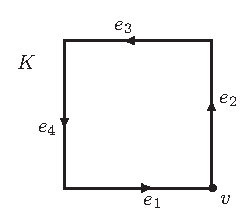
\includegraphics[width=44mm]{figures/1-6-3.pdf}\\图 1.6.3
\end{center}
\entry{例}{1.6.12}考虑图 1.6.4 中的复形 $L$，其底空间为正方形区域，既包括边界，也包括内部。一般的 $1$ 维链为 $c=\sum n_i e_i$。像前例一样推理，可知此链为闭链，当且仅当 $n_1=n_2$、$n_3=n_4$ 且 $n_5=n_3-n_2$。任意指定 $n_2,n_3$ 后，其他系数都随之确定。因此，$Z_1(L)$ 是秩为 $2$ 的自由阿贝尔群。一组可选的基是：取 $n_2=1,n_3=0$ 得到的链 $e_1+e_2-e_5$，以及取 $n_2=0,n_3=1$ 得到的链 $e_3+e_4+e_5$。这组基很方便，因为
\[
\partial_2\sigma_1=e_1+e_2-e_5,\qquad
\partial_2\sigma_2=e_3+e_4+e_5.
\]
因此 $Z_1(L)=B_1(L)$，从而
\[
H_1(L)=Z_1(L)/B_1(L)=0.
\]
\translatornote{原文该等式左边印作 $H_1(K)$，这里依本例复形名称写作 $H_1(L)$。}
还有 $H_2(L)=0$，因为 $L$ 中一般的 $2$ 维链为 $m_1\sigma_1+m_2\sigma_2$，它为闭链，当且仅当 $m_1=m_2=0$。
\begin{center}
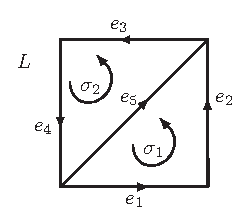
\includegraphics[width=44mm]{figures/1-6-4.pdf}\\图 1.6.4
\end{center}

\sourcepage{36--37}
这些例子或许已使你开始对同调群的几何意义有所体会。只有计算更多例子，才能开始“看见”同调类是什么。我们希望，当你对同调的几何意义有所体会之后，就会开始相信目前还远不清楚的事实：复形 $K$ 的同调群实际上只依赖于底空间 $|K|$。

再来看一个例子，其中单形的数量比前面更多。一般地，单形越多，计算闭链群 $Z_p$ 和边界链群 $B_p$ 就越繁琐。通过跳过这两个群的具体计算，直接计算同调群 $H_p$，可以缩短部分计算过程。

这里仅讨论 $p>0$ 时的群 $H_p(K)$，把 $H_0(K)$ 留到第 1.8 节。

需要引入一些术语。若链 $c$ 在每个不属于子复形 $L$ 的单形上都取值 $0$，则称 $c$ \textbf{由 $L$ 承载}（carried by $L$）。若对于某条 $(p+1)$ 维链 $d$，有 $c-c'=\partial_{p+1}d$，则称两条 $p$ 维链 $c,c'$ \textbf{同调}（homologous）。特别地，若 $c=\partial_{p+1}d$，则称 $c$ \textbf{同调于零}，或简称 $c$ \textbf{是边界}（bounds）。

\entry{例}{1.6.13}考虑图 1.6.5 的复形 $M$，其底空间为正方形区域。我们不具体计算 $1$ 维闭链群，而作如下推理。给定 $1$ 维链 $c$，设其在 $e_1$ 上的值为 $a$。直接计算可得，链
\[
c_1=c+\partial_2(a\sigma_1)
\]
在定向单形 $e_1$ 上取值 $0$。直观地说，通过给 $c$ 加上一个边界，我们已“把它从 $e_1$ 上推开”。接着类似地把 $c_1$ 从 $e_2$ 上推开：令 $b$ 为 $c_1$ 在 $e_2$ 上的值，则
\[
c_2=c_1+\partial_2(b\sigma_2)
\]
在 $e_2$ 上取值 $0$，在 $e_1$ 上也仍取值 $0$，因为 $\partial_2\sigma_2$ 的表达式中没有 $e_1$。再令 $d$ 为 $c_2$ 在 $e_3$ 上的值，则
\[
c_3=c_2+\partial_2(d\sigma_3)
\]
在 $e_3,e_2,e_1$ 上都取值 $0$。这样就把 $c$ 从这三条边上全部推开了。换言之，已经证明：给定 $1$ 维链 $c$，它同调于一条由图 1.6.5 所示 $M$ 的子复形承载的链 $c_3$。\translatornote{此处原文引用图 1.6.5；所说的子复形实际画在图 1.6.6 中。}
\begin{center}
\begin{minipage}{.46\textwidth}\centering
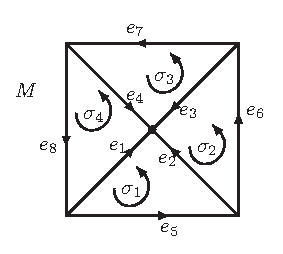
\includegraphics[width=49mm]{figures/1-6-5.pdf}\\图 1.6.5
\end{minipage}\hfill
\begin{minipage}{.46\textwidth}\centering
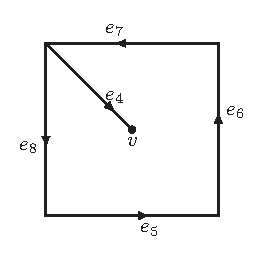
\includegraphics[width=46mm]{figures/1-6-6.pdf}\\图 1.6.6
\end{minipage}
\end{center}
现在，若 $c$ 恰为闭链，则 $c_3$ 也是闭链。因此 $c_3$ 在 $e_4$ 上的值必须为 $0$，否则 $\partial_1c_3$ 在中心顶点 $v$ 上的值便非零。于是，$M$ 中每条 $1$ 维闭链都同调于一条由正方形边界承载的闭链。由例 1.6.11 的论证可知，这样的闭链必为 $e_5+e_6+e_7+e_8$ 的某个整数倍。而后者是边界，事实上，它显然等于 $\partial_2(\sigma_1+\sigma_2+\sigma_3+\sigma_4)$。所以，如所预期，$H_1(M)=0$。

$H_2(M)=0$ 也很容易看出：与前面一样，$\sum m_i\sigma_i$ 为闭链，当且仅当所有 $m_i$ 都为零。

注意，$M$ 的同调群与例 1.6.12 中 $L$ 的同调群相同。这使我们尚未证明的断言更为可信：复形的同调群只依赖于它的底空间。

\entry{定义}{1.6.14}设 $K$ 为复形。$K$ 上的\textbf{无限 $p$ 维链}（infinite $p$-chain）是从 $K$ 的定向 $p$ 维单形集到整数的函数 $c$，满足：若 $\sigma,\sigma'$ 是同一单形的相反定向，则 $c(\sigma)=-c(\sigma')$。不再要求除有限多个单形外均有 $c(\sigma)=0$。无限 $p$ 维链群记为 $C_p^\infty(K)$；它是阿贝尔群，但一般不自由。

\sourcepage{38--39}
定义合适的边界算子 $\partial_p^\infty:C_p^\infty(K)\to C_{p-1}^\infty(K)$ 后，见习题 6，所得群
\[
H_p^\infty(K)=\ker\partial_p^\infty/\operatorname{im}\partial_{p+1}^\infty
\]
称为\textbf{基于无限链的同调群}。

下面的定义将在习题 3 中使用。

\entry{定义}{1.6.15}若一维复形的一维同调为零，则称它为\textbf{树}（tree）。\translatornote{这里保留原书的定义，其中没有要求连通；按通常术语，不连通的这种复形一般称为“森林”。}

\subsection*{习题}
\begin{enumerate}
\item 设 $\mathcal S$ 为由 $1$ 维单形 $\{v_0,v_1\},\{v_1,v_2\},\ldots,\{v_{n-1},v_n\},\{v_n,v_0\}$ 及其顶点组成的抽象复形。若 $K$ 是其几何实现，计算 $H_i(K)$。
\item 考虑图 1.6.7 中的复形 $M$；它是三个三角形与一条线段的并。计算 $H_1(M)$ 与 $H_2(M)$。
\begin{center}
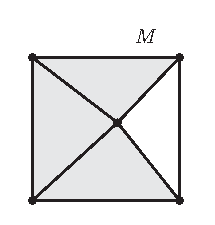
\includegraphics[width=43mm]{figures/1-6-7.pdf}\\图 1.6.7
\end{center}
\item 图 1.6.8 中的两个复形，是否有一个是树？
\begin{center}
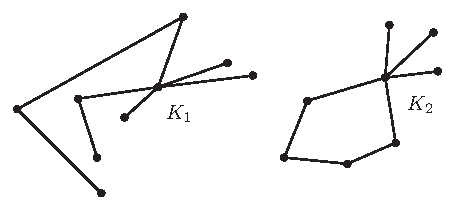
\includegraphics[width=87mm]{figures/1-6-8.pdf}\\图 1.6.8
\end{center}
\item 设 $K$ 为由某个 $3$ 维单形的所有真面组成的复形。计算 $H_1(K)$ 与 $H_2(K)$。
\item 对哪些 $i$ 有 $H_i(K^{(p)})\cong H_i(K)$？
\item \begin{enumerate}[label=(\alph*)]
\item 证明：若 $K$ 局部有限，则可用前面的公式定义边界算子 $\partial_p^\infty:C_p^\infty(K)\to C_{p-1}^\infty(K)$，且引理 1.6.9 仍成立。
\item 设 $K$ 的底空间为 $\R$，顶点为所有整数。证明 $H_1(K)=0$，而 $H_1^\infty(K)\cong\Z$。
\end{enumerate}
\end{enumerate}

\section{曲面的同调群}
\sourcepage{39--40}
若 $K$ 是有限复形，则链群 $C_p(K)$ 的秩有限，因而闭链群 $Z_p(K)$ 的秩也有限。于是 $H_p(K)$ 有限生成，可以应用阿贝尔群基本定理。按照经典术语，$H_p(K)$ 的 Betti 数和挠系数分别称为 $K$ 的 \textbf{$p$ 维 Betti 数}和 \textbf{$p$ 维挠系数}。第二章将证明，这些数是 $|K|$ 的拓扑不变量。

过去，不仅在拓扑学中，在代数学和其他数学领域中，人们也十分重视数值不变量。如今，数学家往往认为同调群是更重要的概念，更倾向于研究这些群的性质，而不是计算其数值不变量。不过，在许多情形下，具体计算同调群，即求出给定空间的 Betti 数与挠系数，仍然很重要。

单纯同调群的最大优点之一，正是这样的计算确实可行。第 1.12 节将证明：有限复形 $K$ 的同调群可以有效计算。这意味着存在求出 $K$ 的 Betti 数与挠系数的具体算法。

本节计算紧致曲面的 Betti 数与挠系数。所用技巧看上去可能有些笨拙，似乎是为特定问题临时设计的；事实上，它们对相当广泛的一类空间都有效。后面研究 CW 复形时，将重新讨论这些技巧，说明它们属于一种系统的同调计算方法。

为明确起见，先定义曲面的含义。

\entry{定义}{1.7.1}\textbf{曲面}（surface）是非空、连通、具有可数基的 Hausdorff 空间 $X$，使得 $X$ 的每个点都有一个与 $\R^2$ 的某个开子集同胚的邻域。

第 4.8 节将定义 $m$ 维流形。依照那里的定义，每个曲面都是二维流形；但由于这里还要求曲面连通且具有可数基，并非每个二维流形都是曲面。

\noindent\textbf{约定：}为简化记号，今后将省略边界算子 $\partial_p$ 的维数下标 $p$，依靠上下文区分所指的算子。

我们将计算环面、Klein 瓶以及其他几个曲面的同调。这些曲面都能通过对矩形 $L$ 的各边作适当等同而构造。因此，先证明关于 $L$ 本身的某些事实。

\entry{引理}{1.7.2}设 $L$ 为图 1.7.1 的复形，其底空间为矩形。用 $\Bd L$ 表示底空间为该矩形边界的复形。把 $L$ 的每个 $2$ 维单形 $\sigma_i$ 都沿逆时针方向定向，任意给各 $1$ 维单形定向。则：
\begin{enumerate}[label=(\arabic*)]
\item $L$ 的每条 $1$ 维闭链都同调于由 $\Bd L$ 承载的某条 $1$ 维闭链。
\item 若 $d$ 是 $L$ 的 $2$ 维链，且 $\partial d$ 由 $\Bd L$ 承载，则 $d$ 是链 $\sum\sigma_i$ 的某个整数倍。
\end{enumerate}
\begin{center}
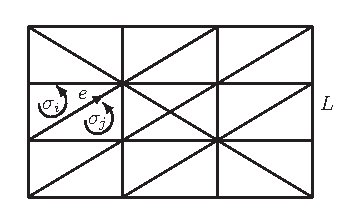
\includegraphics[width=64mm]{figures/1-7-1.pdf}\\图 1.7.1
\end{center}
\noindent\textbf{证明：}(2) 很容易。若 $\sigma_i,\sigma_j$ 有公共边 $e$，则 $\partial d$ 在 $e$ 上的值必须为 $0$。所以 $d$ 在 $\sigma_i$ 与 $\sigma_j$ 上的值相同。不断继续，可知 $d$ 在每个定向 $2$ 维单形上的值都相同。

为证明 (1)，采用例 1.6.13 的方法。给定 $L$ 的 $1$ 维链 $c$，逐步将它从各 $1$ 维单形上推开。先证明 $c$ 同调于由图 1.7.2 的子复形承载的链 $c_1$，再证明 $c_1$ 同调于由图 1.7.3 的子复形承载的链 $c_2$。最后，若原来的 $c$ 为闭链，则 $c_2$ 也为闭链。因此 $c_2$ 必须由 $\Bd L$ 承载，否则它在顶点 $v_1,\ldots,v_5$ 中至少一个上具有非零系数。\translatornote{原文说 $c_2$ 在顶点上有非零系数，按链的维数与论证，应为 $\partial c_2$ 在这些顶点上有非零系数。}\hfill$\square$
\begin{center}
\begin{minipage}{.48\textwidth}\centering
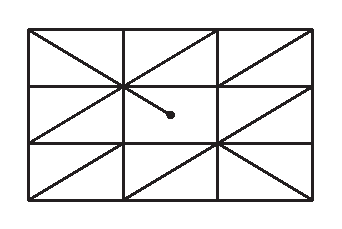
\includegraphics[width=62mm]{figures/1-7-2.pdf}\\图 1.7.2
\end{minipage}\hfill
\begin{minipage}{.48\textwidth}\centering
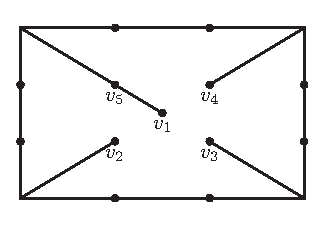
\includegraphics[width=60mm]{figures/1-7-3.pdf}\\图 1.7.3
\end{minipage}
\end{center}

\sourcepage{41--42}
\entry{定理}{1.7.3}设 $T$ 为图 1.7.4 的带标记矩形 $L$ 表示的复形，其底空间为环面。则
\[
H_1(T)\cong\Z\oplus\Z,\qquad H_2(T)\cong\Z.
\]
将 $L$ 的每个 $2$ 维单形沿逆时针方向定向，并用诱导的定向给 $T$ 的各 $2$ 维单形定向，以 $\gamma$ 表示它们的和。令
\[
\begin{aligned}
w_1&=[a,b]+[b,c]+[c,a],\\
z_1&=[a,d]+[d,e]+[e,a].
\end{aligned}
\]
则 $\gamma$ 生成 $H_2(T)$，而 $w_1,z_1$ 代表 $H_1(T)$ 的一组基。
\begin{center}
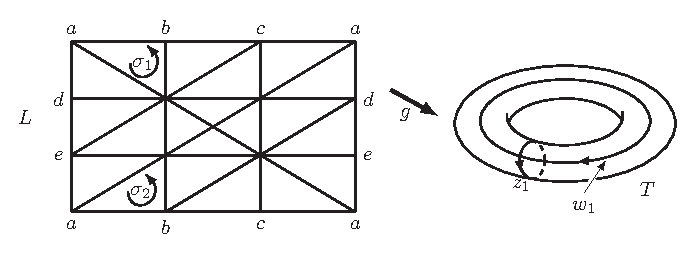
\includegraphics[width=119mm]{figures/1-7-4.pdf}\\图 1.7.4
\end{center}
\noindent\textbf{证明：}设 $g:|L|\to|T|$ 为粘合映射，$A=g(|\Bd L|)$。则 $A$ 同胚于两个只有一个公共点的圆周的并，这种空间称为\textbf{两个圆周的楔和}（wedge）。任意给 $T$ 的各 $1$ 维单形定向。因为 $g$ 只在 $\Bd L$ 的单形之间进行等同，引理 1.7.2 的论证可原样用于证明：
\begin{enumerate}[label=(\arabic*)]
\item $T$ 的每条 $1$ 维闭链都同调于由 $A$ 承载的 $1$ 维闭链。
\item 若 $d$ 为 $T$ 的 $2$ 维链，且 $\partial d$ 由 $A$ 承载，则 $d$ 是 $\gamma$ 的整数倍。
\end{enumerate}
另外，$T$ 中还有：
\begin{enumerate}[label=(\arabic*),start=3]
\item 若 $c$ 为由 $A$ 承载的 $1$ 维闭链，则 $c$ 形如 $nw_1+mz_1$。
\item $\partial\gamma=0$。
\end{enumerate}
由于 $A$ 就是图 1.7.5 的一维复形，(3) 很容易证明。(4) 也很直接：显然，$\partial\gamma$ 在所有不属于 $A$ 的 $1$ 维单形上都取值 $0$。直接检验可知，它在属于 $A$ 的每个 $1$ 维单形上也取值 $0$。例如，初等链 $[a,b]$ 在 $\partial\sigma_1$ 中的系数为 $-1$，在 $\partial\sigma_2$ 中的系数为 $+1$，所以 $\partial\gamma$ 在 $[a,b]$ 上取值 $0$，见图 1.7.4。$w_1,z_1$ 中其他定向 $1$ 维单形也有类似结论。
\begin{center}
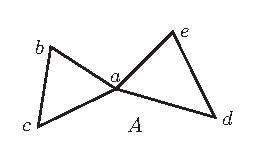
\includegraphics[width=48mm]{figures/1-7-5.pdf}\\图 1.7.5
\end{center}
利用 (1)--(4) 即可计算 $T$ 的同调。由 (1) 和 (3)，每条 $1$ 维闭链都同调于形如 $nw_1+mz_1$ 的闭链。这种闭链只有为零时才是边界：若 $c=\partial d$，由 (2) 得 $d=q\gamma$，再由 (4) 得 $c=\partial d=0$。所以 $H_1(T)\cong\Z\oplus\Z$，闭链 $w_1,z_1$ 的陪集构成一维同调的一组基。

为计算 $H_2(T)$，注意由 (2)，每条 $2$ 维闭链 $d$ 必定形如 $q\gamma$；由 (4)，每条这样的 $2$ 维链确为闭链，而且没有 $3$ 维链能以它为边界。所以 $H_2(T)\cong\Z$，由 $2$ 维闭链 $\gamma$ 生成。\hfill$\square$

\sourcepage{43--44}
\entry{定理}{1.7.4}设 $S$ 为图 1.7.6 的带标记矩形表示的复形，其底空间为 Klein 瓶。则
\[
H_1(S)\cong\Z\oplus\Z/2,\qquad H_2(S)=0.
\]
$H_1(S)$ 的挠元素由链 $z_1$ 代表，而将挠子群除去后的群的一个生成元由 $w_1$ 代表，其中
\[
w_1=[a,b]+[b,c]+[c,a],\qquad z_1=[a,d]+[d,e]+[e,a].
\]
\begin{center}
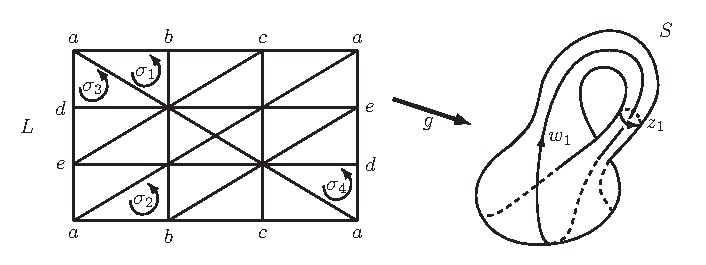
\includegraphics[width=121mm]{figures/1-7-6.pdf}\\图 1.7.6
\end{center}
\noindent\textbf{证明：}与定理 1.7.3 一样，令 $g:|L|\to|S|$ 为粘合映射，$A=g(|\Bd L|)$。$A$ 仍是两个圆周的楔和。将 $S$ 的各 $2$ 维单形沿逆时针方向定向，令其和为 $\gamma$；任意给各 $1$ 维单形定向。定理 1.7.3 证明中的 (1)、(2) 仍成立，因为它们不涉及边界上的具体等同方式。因为 $A$ 为两个圆周的楔和，(3) 也成立。最后的 (4) 改为
\[
\text{(4)}\qquad\partial\gamma=2z_1.
\]
直接计算即可验证。例如，$[a,b]$ 在 $\partial\sigma_1$ 中的系数为 $-1$，在 $\partial\sigma_2$ 中为 $+1$；而 $[a,d]$ 在 $\partial\sigma_3$ 和 $\partial\sigma_4$ 中的系数都为 $+1$。$w_1,z_1$ 中其他定向边也有类似结论。

综合这些事实，由 (1)、(3)，$S$ 的每条 $1$ 维闭链都同调于形如 $nw_1+mz_1$ 的闭链。若 $c=\partial d$，由 (2) 得 $d=p\gamma$，由 (4) 得 $\partial d=2pz_1$。因此，$nw_1+mz_1$ 为边界，当且仅当 $m$ 为偶数且 $n=0$。所以 $H_1(S)\cong\Z\oplus\Z/2$。闭链 $z_1$ 代表挠元素，$w_1$ 代表无限循环群 $H_1(S)/T_1(S)$ 的一个生成元。

由 (2)，$S$ 的每条 $2$ 维闭链都形如 $p\gamma$；由 (4)，当 $p\ne0$ 时它不是闭链，故 $H_2(S)=0$。\hfill$\square$

\entry{定理}{1.7.5}设 $P^2$ 为图 1.7.7 的带标记矩形所指定的复形。由例 1.4.10，其底空间称为射影平面。则
\[
H_1(P^2)\cong\Z/2,\qquad H_2(P^2)=0.
\]
\begin{center}
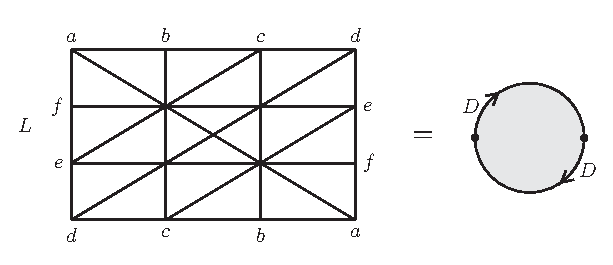
\includegraphics[width=107mm]{figures/1-7-7.pdf}\\图 1.7.7
\end{center}
\noindent\textbf{证明：}设 $g:|L|\to|P^2|$ 为粘合映射，$A=g(\Bd L)$，则 $A$ 同胚于圆周。与前两个定理一样定义 $\gamma$，令
\[
z_1=[a,b]+[b,c]+[c,d]+[d,e]+[e,f]+[f,a].
\]
定理 1.7.3 证明中的 (1)、(2) 仍成立。此外，容易验证：
\begin{enumerate}[label=(\arabic*),start=3]
\item 每条由 $A$ 承载的 $1$ 维闭链都是 $z_1$ 的整数倍。
\item $\partial\gamma=-2z_1$。
\end{enumerate}
于是 $H_1(P^2)\cong\Z/2$，$H_2(P^2)=0$。$H_1$ 的非零元素由闭链 $z_1$ 代表。\hfill$\square$

\sourcepage{45--46}
\entry{定义}{1.7.6}两个曲面 $S_1,S_2$ 的\textbf{连通和}（connected sum）定义为如下得到的曲面：从每个曲面中删去一个小开圆盘，再沿剩余部分的自由边界将它们粘合。记此空间为 $S_1\mathbin{\#}S_2$。

设 $T$ 为环面，空间 $T\mathbin{\#}T$ 称为\textbf{双环面}，如图 1.7.8。
\begin{center}
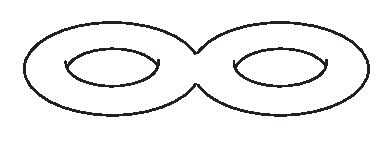
\includegraphics[width=69mm]{figures/1-7-8.pdf}\\图 1.7.8
\end{center}
空间 $P^2\mathbin{\#}P^2$ 可以表示为按图 1.7.9 所示方式粘合矩形各边所得到的商空间。注意，沿虚线 $C$ 剪开矩形，就得到图中所示的两个各自删去了一个开圆盘的射影平面。
\begin{center}
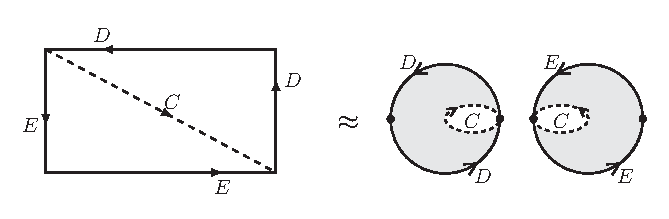
\includegraphics[width=116mm]{figures/1-7-9.pdf}\\图 1.7.9
\end{center}
\entry{定理}{1.7.7}设 $P^2\mathbin{\#}P^2$ 为两个射影平面的连通和。则
\[
H_1(P^2\mathbin{\#}P^2)\cong\Z\oplus\Z/2,\qquad
H_2(P^2\mathbin{\#}P^2)=0.
\]
\noindent\textbf{证明：}仍用前面的矩形 $L$ 表示 $P^2\mathbin{\#}P^2$，给顶点作与图 1.7.8 一致的标记。\translatornote{原文此处引用图 1.7.8，据粘合方式应为图 1.7.9。}此时复形 $A=g(|\Bd L|)$ 仍为两个圆周的楔和。令 $w_1$ 为沿矩形上边从右向左的 $1$ 维闭链，$z_1$ 为沿左边从上向下的 $1$ 维闭链，如图 1.7.9。定理 1.7.3 证明中的 (1)、(2) 仍成立，并且：
\begin{enumerate}[label=(\arabic*),start=3]
\item 每条由 $A$ 承载的 $1$ 维闭链都形如 $nw_1+mz_1$。
\item $\partial\gamma=2w_1+2z_1$。
\end{enumerate}
由此显然有 $H_2(P^2\mathbin{\#}P^2)=0$，但计算 $H_1$ 还需要进一步工作。

需要将以 $w_1,z_1$ 为基的群 $G$，对由 $2(w_1+z_1)$ 生成的子群 $H$ 取商。为此，要像自由阿贝尔群子群的基本定理 1.5.2 那样，为两群选择“相容”的基。此处容易看出，应使 $w_1+z_1$ 成为 $G$ 的一个基元素。确实可以做到：$\{w_1,w_1+z_1\}$ 与 $\{w_1,z_1\}$ 一样都是基，因为 $z_1=-w_1+(w_1+z_1)$，两组基可彼此表示。使用新基，便清楚地得到
\[
H_1(P^2\mathbin{\#}P^2)\cong\Z\oplus\Z/2.
\]
挠元素由 $w_1+z_1$ 代表，$w_1$ 代表 $H_1/T_1$ 的一个生成元。

注意，$w_1$ 不是唯一能代表 $H_1/T_1$ 的生成元的闭链。$z_1$ 也可以，因为 $\{z_1,w_1+z_1\}$ 是 $G$ 的一组基。同样，$\{2w_1+3z_1,w_1+z_1\}$ 也是基，因此 $2w_1+3z_1$ 也代表 $H_1/T_1$ 的一个生成元。事实上还有许多这样的闭链。\hfill$\square$

细心的读者可能注意到，这里的同调群与 Klein 瓶的同调群相同，见定理 1.7.4。这并非偶然，因为这两个空间实际上同胚，图 1.7.10 给出了证明示意。
\begin{center}
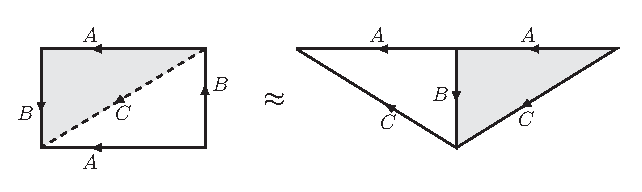
\includegraphics[width=113mm]{figures/1-7-10.pdf}\\图 1.7.10
\end{center}
\entry{定义}{1.7.8}图 1.7.11 所示的商空间称为\textbf{笨帽空间}（dunce cap）。
\begin{center}
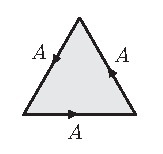
\includegraphics[width=31mm]{figures/1-7-11.pdf}\\图 1.7.11
\end{center}
习题 6 将推广笨帽空间。

下面的定理是十九世纪数学的一项重大成就。

\sourcepage{47--48}
\entry{定理}{1.7.9（紧致曲面分类定理）}每个紧致曲面都同胚于球面、$n$ 个环面的连通和，或 $m$ 个射影平面的连通和。

这里不证明此定理；可参阅 [Mun00] 第 12 章。

根据分类定理和已经算过的例子，你应当能够计算一般紧致曲面的同调群。此计算留作习题。

\subsection*{习题}
\begin{enumerate}
\item 设 $w_1,z_1$ 为图 1.7.6 中 Klein 瓶上的闭链。证明 $w_1+z_1$ 代表无限循环群 $H_1(S)/T_1(S)$ 的一个生成元。
\item 两个环面的连通和 $T\mathbin{\#}T$ 可表示为平面八边形区域的商空间，其中边界按图 1.7.12 等同。沿虚线分开八边形，就得到两个各自删去了开圆盘的环面。
\begin{enumerate}[label=(\alph*)]
\item 给图 1.7.13 中复形 $L$ 的顶点适当标记，构造底空间为 $T\mathbin{\#}T$ 的复形 $K$。
\item 仿照定理 1.7.3 计算 $T\mathbin{\#}T$ 的同调。具体地，令 $A$ 为 $\Bd L$ 在商映射下的像，则 $A$ 是四个圆周的楔和。将 $L$ 的每个 $2$ 维单形逆时针定向，令 $\gamma$ 为 $K$ 中相应定向单形的和。证明每条 $1$ 维闭链都同调于由 $A$ 承载的闭链；再证明每条边界由 $A$ 承载的 $2$ 维链都是 $\gamma$ 的整数倍。最后，分析由 $A$ 承载的 $1$ 维闭链，并计算 $\partial\gamma$，完成同调计算。
\end{enumerate}
\begin{center}
\begin{minipage}{.46\textwidth}\centering
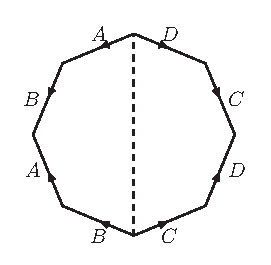
\includegraphics[width=49mm]{figures/1-7-12.pdf}\\图 1.7.12
\end{minipage}\hfill
\begin{minipage}{.46\textwidth}\centering
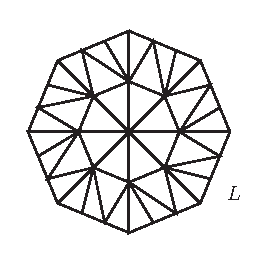
\includegraphics[width=47mm]{figures/1-7-13.pdf}\\图 1.7.13
\end{minipage}
\end{center}
\item 对图 1.7.12 中的复形 $L$ 作适当标记，表示四重连通和 $P^2\mathbin{\#}P^2\mathbin{\#}P^2\mathbin{\#}P^2$，并计算其一维、二维同调。\translatornote{原文引用图 1.7.12，但复形 $L$ 实际画在图 1.7.13。}
\item \begin{enumerate}[label=(\alph*)]
\item 定义 $n$ 个环面的连通和 $X_n=T\mathbin{\#}T\mathbin{\#}\cdots\mathbin{\#}T$，并计算一维、二维同调。
\item 定义 $n$ 个射影平面的连通和 $Y_n=P^2\mathbin{\#}\cdots\mathbin{\#}P^2$，并计算一维、二维同调。
\end{enumerate}
\item 计算 $T\mathbin{\#}P^2$ 的同调。它必同胚于习题 4 所列的哪个曲面？能否构造这个同胚？
\item \begin{enumerate}[label=(\alph*)]
\item 计算图 1.7.14 所示商空间的一维、二维同调。称此空间为“五重笨帽空间”。
\item 类似地定义“$k$ 重笨帽空间”，并计算其同调。
\end{enumerate}
\begin{center}
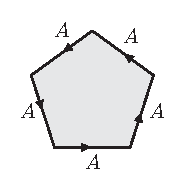
\includegraphics[width=35mm]{figures/1-7-14.pdf}\\图 1.7.14
\end{center}
\item 计算图 1.7.15 所示空间的同调。
\begin{center}
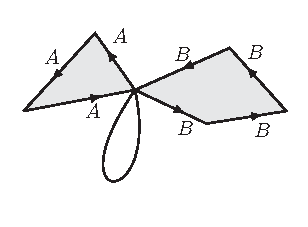
\includegraphics[width=58mm]{figures/1-7-15.pdf}\\图 1.7.15
\end{center}
\item 给定有限生成阿贝尔群 $G_1,G_2$，其中 $G_2$ 自由，证明存在有限二维复形 $K$，使 $|K|$ 连通，$H_1(K)\cong G_1$ 且 $H_2(K)\cong G_2$。
\end{enumerate}

\section{零维同调}
\sourcepage{48--49}
我们还没有计算过零维同调群。本节将说明，这个群有简单的拓扑解释，因此计算起来十分容易。

\entry{定理}{1.8.1}设 $K$ 为复形，则 $H_0(K)$ 是自由阿贝尔群。若顶点族 $\{v_\alpha\}$ 在 $|K|$ 的每个连通分支中恰好选取一个顶点，则各链 $v_\alpha$ 的同调类构成 $H_0(K)$ 的一组基。

\noindent\textbf{证明：}
\textbf{第一步。}对于 $K$ 的顶点 $v,w$，若存在一列顶点 $a_0,a_1,\ldots,a_n$，使 $v=a_0,w=a_n$，且每个 $a_i a_{i+1}$ 都是 $K$ 的一个 $1$ 维单形，则定义 $v\sim w$。这显然是等价关系。给定 $v$，令
\[
C_v=\bigcup\{\operatorname{St}w:w\sim v\}.
\]
下面证明，这些集合就是 $|K|$ 的连通分支。

首先，$C_v$ 是开集，因为它是开集的并。而且，若 $v\sim v'$，则 $C_v=C_{v'}$。

其次，$C_v$ 连通，实际上它道路连通。设 $w\sim v$，$x\in\operatorname{St}w$，像前面一样选择顶点列 $a_0,\ldots,a_n$。依次连接 $a_0,a_1,\ldots,a_n,x$ 的折线路径位于 $C_v$ 中：根据定义，$a_i\sim v$，所以 $\operatorname{St}a_i\subset C_v$，特别地，线段 $a_i a_{i+1}$ 位于 $C_v$。同样，线段 $a_nx$ 位于 $\operatorname{St}a_n\subset C_v$。因此 $C_v$ 道路连通。

第三，证明不同的集合 $C_v,C_{v'}$ 不相交。若 $x\in C_v\cap C_{v'}$，则存在 $w\sim v$、$w'\sim v'$，使 $x\in\operatorname{St}w\cap\operatorname{St}w'$。由于 $x$ 关于 $w,w'$ 的重心坐标均为正，$K$ 的某个单形以 $w,w'$ 为顶点。于是 $ww'$ 是 $K$ 的 $1$ 维单形，故 $w\sim w'$。所以 $v\sim v'$，两集合相同。

这些集合连通、开且两两不相交，必是 $|K|$ 的连通分支。注意，每个分支都是 $K$ 的某个子复形的底空间：$K$ 的每个单形由于连通，都完全位于某一个分支中。

\sourcepage{50}
\textbf{第二步。}现在证明定理。设 $\{v_\alpha\}$ 从每个连通分支 $C_\alpha$ 中选取一个顶点。给定 $K$ 的顶点 $w$，设它位于 $C_\alpha$。根据假设，$w\sim v_\alpha$，因此存在从 $v_\alpha$ 到 $w$ 的顶点列 $a_0,\ldots,a_n$。$1$ 维链
\[
[a_0,a_1]+[a_1,a_2]+\cdots+[a_{n-1},a_n]
\]
的边界为 $a_n-a_0=w-v_\alpha$。所以 $0$ 维链 $w$ 同调于 $v_\alpha$。由此，$K$ 中每条 $0$ 维链都同调于初等 $0$ 维链 $v_\alpha$ 的某个线性组合。

最后证明，形如 $c=\sum n_\alpha v_\alpha$ 的非零 $0$ 维链不可能是边界。设 $c=\partial d$，其中 $d$ 为 $1$ 维链。由于 $K$ 的每个 $1$ 维单形只位于 $|K|$ 的一个分支中，可以写成 $d=\sum d_\alpha$，其中 $d_\alpha$ 由 $d$ 中那些由 $C_\alpha$ 承载的项组成。因 $\partial d=\sum\partial d_\alpha$，且每个 $\partial d_\alpha$ 由 $C_\alpha$ 承载，所以 $\partial d_\alpha=n_\alpha v_\alpha$。于是每个 $n_\alpha=0$。具体地，定义同态 $\epsilon:C_0(K)\to\Z$，使对每个顶点 $v$ 有 $\epsilon(v)=1$。则
\[
\epsilon(\partial[v,w])=\epsilon(w-v)=1-1=0.
\]
所以对每条 $1$ 维链 $e$，都有 $\epsilon(\partial e)=0$。特别地，
\[
0=\epsilon(\partial d_\alpha)=\epsilon(n_\alpha v_\alpha)=n_\alpha.
\]\hfill$\square$

在某些问题中，使用零维同调的另一种形式更加方便，下面讨论这种形式。

\entry{定义}{1.8.2}令满同态 $\epsilon:C_0(K)\to\Z$ 由每个顶点上的取值 $\epsilon(v)=1$ 定义。若 $c$ 为 $0$ 维链，则 $\epsilon(c)$ 等于 $c$ 在各顶点上取值的总和。$\epsilon$ 称为 $C_0(K)$ 的\textbf{增广映射}（augmentation map）。上一个证明已说明，若 $d$ 为 $1$ 维链，则 $\epsilon(\partial d)=0$。定义 $K$ 的\textbf{零维约化同调群}（reduced homology group）为
\[
\widetilde H_0(K)=\ker\epsilon/\operatorname{im}\partial_1.
\]
若 $p>0$，则令 $\widetilde H_p(K)$ 表示通常的 $H_p(K)$。

约化同调与普通同调的关系如下。

\entry{定理}{1.8.3}群 $\widetilde H_0(K)$ 是自由阿贝尔群，且
\[
\widetilde H_0(K)\oplus\Z\cong H_0(K).\tag{$*$}
\]
因此，若 $|K|$ 连通，则 $\widetilde H_0(K)=0$。若 $|K|$ 不连通，从其每个分支选取一个顶点，组成族 $\{v_\alpha\}$，并固定指标 $\alpha_0$，则各链 $v_\alpha-v_{\alpha_0}$（$\alpha\ne\alpha_0$）的同调类构成 $\widetilde H_0(K)$ 的一组基。

\noindent\textbf{证明：}同前，在每个分支中选取顶点 $v_\alpha$。给定 $0$ 维链 $c$，它同调于形如 $c'=\sum n_\alpha v_\alpha$ 的链，且后者只有在所有 $n_\alpha=0$ 时才为边界。另一方面，若 $c\in\ker\epsilon$，则
\[
\epsilon(c)=\epsilon(c')=\epsilon\left(\sum n_\alpha v_\alpha\right)=\sum n_\alpha=0.
\]
若 $|K|$ 只有一个分支，则 $c\in\ker\epsilon$ 蕴含 $c'=0$，故 $\widetilde H_0(K)=0$。由定理 1.8.1，$H_0(K)\cong\Z$，从而验证了 $(*)$。

\sourcepage{51}
若 $|K|$ 有多于一个分支，则 $c\in\ker\epsilon$ 蕴含 $c'$ 是 $v_\alpha-v_{\alpha_0}$（$\alpha\ne\alpha_0$）的线性组合。再次应用定理 1.8.1 即得 $(*)$。\hfill$\square$

\subsection*{习题}
\begin{enumerate}
\item \begin{enumerate}[label=(\alph*)]
\item 设 $G$ 为阿贝尔群，$\varphi:G\to\Z$ 为满同态。证明 $G$ 有一个无限循环子群 $H$，使 $G=(\ker\varphi)\oplus H$。［提示：构造同态 $\psi:\Z\to G$，使 $\varphi\circ\psi$ 为恒等映射，令 $H=\operatorname{im}\psi$。］
\item 证明：若 $\varphi:C_0\to\Z$ 是任意满足 $\varphi\circ\partial_1=0$ 的满同态，则
\[
H_0(K)\cong(\ker\varphi)/(\operatorname{im}\partial_1)\oplus\Z.
\]
\end{enumerate}
\end{enumerate}

\section{锥的同调}
\sourcepage{51--52}
现在计算 $n$ 维单形及其边界的同调。为方便起见，先引入锥的概念。

\entry{定义}{1.9.1}设 $K$ 是 $E^J$ 中的复形，$w\in E^J$，且从 $w$ 出发的每条射线与 $|K|$ 至多相交于一点。定义\textbf{以 $w$ 为顶点的 $K$ 上的锥}（cone），为所有形如 $wa_0a_1\cdots a_p$ 的单形及其所有面构成的族，其中 $a_0a_1\cdots a_p$ 为 $K$ 的单形。记作 $w*K$，见图 1.9.1。\translatornote{锥的这一几何构造还需假定 $w\notin|K|$；原文未单独明说。}
\begin{center}
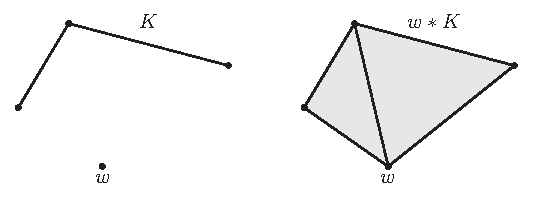
\includegraphics[width=96mm]{figures/1-9-1.pdf}\\图 1.9.1
\end{center}
下面说明 $w*K$ 是良定义的复形，并包含 $K$ 为子复形。$K$ 常称为锥的\textbf{底}（base）。

先证明点集 $\{w,a_0,a_1,\ldots,a_p\}$ 几何独立。若 $w$ 位于 $a_0,\ldots,a_p$ 确定的平面 $P$ 中，考察连接 $w$ 与 $\sigma=a_0\cdots a_p$ 的内点 $x$ 的线段。由于 $\Int\sigma$ 在 $P$ 中开，它包含这条线段上的一个区间。但根据假设，从 $w$ 经过 $x$ 的射线与 $|K|$ 只有一个交点，矛盾。

再证明 $w*K$ 是复形。其单形有三类：$K$ 的单形 $a_0\cdots a_p$，形如 $wa_0\cdots a_p$ 的单形，以及 $0$ 维单形 $w$。第一类的不同单形内部不交，因为 $K$ 是复形。开单形 $\Int(wa_0\cdots a_p)$ 是连接 $w$ 与 $\Int(a_0\cdots a_p)$ 中各点的所有开线段的并；这样的两个开单形不能相交，因为从 $w$ 出发的任何射线都不会包含 $|K|$ 中多于一个点。同理，第一类与第二类单形的内部也不相交。

\entry{例}{1.9.2}设 $K_\sigma$ 是由单形 $\sigma=v_0v_1\cdots v_n$ 及其各面组成的复形，则 $K_\sigma=v_0*K_s$，其中 $s$ 是 $\sigma$ 中与 $v_0$ 相对的面。因此，每个正维单形都是锥。

\entry{例}{1.9.3}设 $K$ 是 $\R^2$ 中由 $x$ 轴上的区间 $[n,n+1]\times0$ 及其顶点组成的复形，$w$ 是 $y$ 轴上不同于原点的一点。则 $w*K$ 为图 1.9.2 的复形。虽然 $|K|$ 是 $\R^2$ 的子空间，$|w*K|$ 却不是，见第 1.3 节习题 9。
\begin{center}
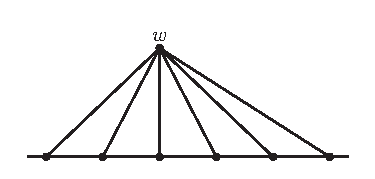
\includegraphics[width=68mm]{figures/1-9-2.pdf}\\图 1.9.2
\end{center}
锥构造的一个特别有用的推论如下。

\entry{引理}{1.9.4}设 $U$ 是 $\R^n$ 中的有界凸开集，$w\in U$。若 $K$ 是满足 $|K|=\overline U\setminus U$ 的有限复形，则 $w*K$ 为有限复形，且 $|w*K|=\overline U$。

\noindent\textbf{证明：}由引理 1.2.7，从 $w$ 出发的每条射线与 $|K|$ 恰好相交于一点，而且 $\overline U$ 是连接 $w$ 与 $|K|$ 中各点的所有线段的并。\hfill$\square$

\sourcepage{53}
给定 $K$，其上的任意两个锥 $w*K$、$z*K$ 同构：将 $K$ 的各顶点映到自身，并将 $w$ 映到 $z$ 的顶点映射，诱导了这两个锥之间的同构。

注意，对于 $\R^N$ 中的复形 $K$，可能不存在 $\R^N$ 中的点 $w$ 使锥 $w*K$ 能够构成。不过，总可以将 $K$ 视为 $\R^N\times0\subset\R^{N+1}$ 中的复形，此时取 $w=(0,0,\ldots,0,1)\in\R^{N+1}$ 即可。对 $E^J$ 中的复形也有类似结论。

下面计算锥的同调，证明其正维同调均为零。为此引入一种括号运算，后文也将用到。

\entry{定义}{1.9.5}设 $w*K$ 为锥。若 $\sigma=[a_0,a_1,\ldots,a_p]$ 是 $K$ 的定向单形，以 $[w,\sigma]$ 表示 $w*K$ 的定向单形 $[w,a_0,a_1,\ldots,a_p]$。此运算良定义：交换序列 $[a_0,\ldots,a_p]$ 中两个顶点，恰好也交换 $[w,a_0,\ldots,a_p]$ 中两个顶点。更一般地，若 $c_p=\sum n_i\sigma_i$ 是 $K$ 的 $p$ 维链，定义
\[
[w,c_p]=\sum n_i[w,\sigma_i].
\]
这个括号运算是将 $C_p(K)$ 映入 $C_{p+1}(w*K)$ 的同态。\translatornote{原文将目标写作 $C_{p+1}(K)$，但加上顶点 $w$ 后的单形属于锥 $w*K$。}
由边界公式容易计算：
\[
\partial[w,\sigma]=\begin{cases}
\sigma-w,&\dim\sigma=0,\\
\sigma-[w,\partial\sigma],&\dim\sigma>0.
\end{cases}
\]
从而得到更一般的公式：
\[
\partial[w,c_0]=c_0-\epsilon(c_0)w,\qquad
\partial[w,c_p]=c_p-[w,\partial c_p]\quad(p>0).
\]
\entry{定理}{1.9.6}若 $w*K$ 是锥，则对所有 $p$ 都有 $\widetilde H_p(w*K)=0$。

一般地，若复形在所有维数上的约化同调都为零，就称其为\textbf{无环的}（acyclic）。

\sourcepage{54}
\noindent\textbf{证明：}由于 $|w*K|$ 连通，其零维约化同调为零。设 $p>0$，取 $w*K$ 的 $p$ 维闭链 $z_p$，证明它是边界。写作
\[
z_p=c_p+[w,d_{p-1}],
\]
其中 $c_p$ 由 $z_p$ 中那些由 $K$ 承载的项组成，$d_{p-1}$ 为 $K$ 的链。只需证明 $z_p-\partial[w,c_p]=0$。直接计算得
\[
\begin{aligned}
z_p-\partial[w,c_p]
&=c_p+[w,d_{p-1}]-c_p+[w,\partial c_p]\\
&=[w,e_{p-1}],
\end{aligned}
\]
其中 $e_{p-1}=d_{p-1}+\partial c_p$ 是 $K$ 的链。\translatornote{原文定义该链时左端下标印作 $e_p$，据维数与后文应为 $e_{p-1}$。}因为 $z_p$ 是闭链，对上式取边界得
\[
0=\begin{cases}
e_{p-1}-\epsilon(e_{p-1})w,&p=1,\\
e_{p-1}-[w,\partial e_{p-1}],&p>1.
\end{cases}
\]
这个链中由 $K$ 承载的部分只有 $e_{p-1}$，故 $e_{p-1}=0$。所以
\[
z_p-\partial[w,c_p]=[w,e_{p-1}]=0,
\]
得到所需结论。\hfill$\square$

\entry{定理}{1.9.7}设 $\sigma$ 为 $n$ 维单形，则由 $\sigma$ 及其各面构成的复形 $K_\sigma$ 无环。若 $n>0$，令 $\Sigma^{n-1}$ 为多胞体等于 $\Bd\sigma$ 的复形，并给 $\sigma$ 定向。则 $\widetilde H_{n-1}(\Sigma^{n-1})$ 为无限循环群，由链 $\partial\sigma$ 生成；当 $i\ne n-1$ 时，$\widetilde H_i(\Sigma^{n-1})=0$。

回顾引理 1.2.6，$\Bd\sigma$ 同胚于 $S^{n-1}$，所以此定理给出了球面的同调。

\noindent\textbf{证明：}由于 $K_\sigma$ 是锥，它无环，见例 1.9.2。\translatornote{此论证直接适用于 $n>0$；当 $n=0$ 时，$K_\sigma$ 是单点复形，其约化同调直接由定义为零。}比较 $K_\sigma$ 与 $\Sigma^{n-1}$ 的链群，除 $n$ 维外，它们相同。下图保留边界算子的维数下标，并区分两个复形的边界算子：
\[
\begin{array}{ccccccccc}
C_n(K_\sigma)&\xrightarrow{\partial_n}&C_{n-1}(K_\sigma)&\xrightarrow{\partial_{n-1}}&\cdots&\xrightarrow{\partial_1}&C_0(K_\sigma)&\xrightarrow{\epsilon}&\Z\\
&&\Vert&&&&\Vert&&\Vert\\
0&\xrightarrow{\partial'_n}&C_{n-1}(\Sigma^{n-1})&\xrightarrow{\partial'_{n-1}}&\cdots&\xrightarrow{\partial'_1}&C_0(\Sigma^{n-1})&\longrightarrow&\Z.
\end{array}
\]
立即得 $i\ne n-1$ 时，$\widetilde H_i(\Sigma^{n-1})=\widetilde H_i(K_\sigma)=0$。

\sourcepage{55--56}
再算 $n-1$ 维同调。先设 $n>1$。由于 $C_n(\Sigma^{n-1})$ 为平凡群，$C_{n-1}(\Sigma^{n-1})$ 中没有非零边界。于是
\[
\begin{aligned}
H_{n-1}(\Sigma^{n-1})&=Z_{n-1}(\Sigma^{n-1})\\
&=\ker\partial'_{n-1}=\ker\partial_{n-1}\\
&=\operatorname{im}\partial_n,
\end{aligned}
\]
最后一步因为 $H_{n-1}(K_\sigma)=0$。$C_n(K_\sigma)$ 为由 $\sigma$ 生成的无限循环群，所以 $\operatorname{im}\partial_n$ 是由 $\partial_n\sigma$ 生成的循环群；因为 $C_{n-1}(K_\sigma)$ 无挠，它为无限群。

$n=1$ 的论证类似，只需始终将 $\partial_{n-1}$ 换为 $\epsilon$。\hfill$\square$

下面的定义在习题中要用到；“悬挂”的概念也将在后面各节再次出现。

\entry{定义}{1.9.8}设 $K$ 为复形，$w_0*K$、$w_1*K$ 为其上的两个锥，且其多胞体仅在 $|K|$ 相交。习题 1(a) 要求证明 $(w_0*K)\cup(w_1*K)$ 是复形，称为 $K$ 的一个\textbf{悬挂}（suspension），记为 $S(K)$，见图 1.9.3。
\begin{center}
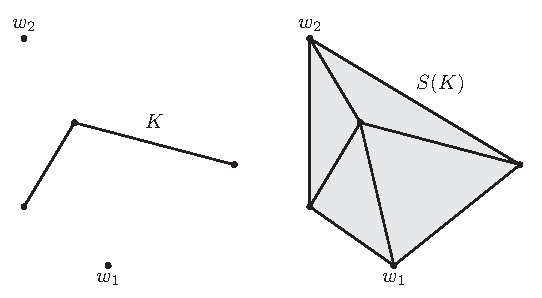
\includegraphics[width=98mm]{figures/1-9-3.pdf}\\图 1.9.3
\end{center}
\subsection*{习题}
\begin{enumerate}
\item 设 $K$ 为复形，$w_0*K$、$w_1*K$ 为两个多胞体仅在 $|K|$ 相交的锥。
\begin{enumerate}[label=(\alph*)]
\item 证明 $(w_0*K)\cup(w_1*K)$ 是复形。
\item 用括号记号，按公式 $\varphi(c_p)=[w_0,c_p]-[w_1,c_p]$ 定义 $\varphi:C_p(K)\to C_{p+1}(S(K))$。证明 $\varphi$ 诱导同态
\[
\varphi_*:\widetilde H_p(K)\longrightarrow\widetilde H_{p+1}(S(K)).
\]
\item 证明：若 $K$ 由一个 $2$ 维单形的所有真面组成，则 $\varphi_*$ 是同构。
\end{enumerate}
后面将看到，一般情况下 $\varphi_*$ 也是同构，见第 3.4 节。
\end{enumerate}

\section{相对同调}
\sourcepage{56--57}
设 $K_0$ 为复形 $K$ 的子复形。在拓扑学的许多应用中，考虑所谓 $K$ 模 $K_0$ 的相对同调群很方便。这里先简要介绍并计算一些例子，把更完整的讨论留到第三章。

链群 $C_p(K_0)$ 可以自然地视为 $C_p(K)$ 的子群。形式上说，若 $c_p$ 是 $K_0$ 上的链，即定义在 $K_0$ 的定向单形上的函数，可令其在 $K$ 中所有不属于 $K_0$ 的定向 $p$ 维单形上取值 $0$，从而扩张为 $K$ 上的链。若把 $c_p$ 写成 $K_0$ 的定向单形的线性组合，则只需将这些单形也视为属于 $K$，就把 $c_p$ 视为了 $K$ 的链。

\entry{定义}{1.10.1}若 $K_0$ 为 $K$ 的子复形，称 $(K,K_0)$ 为\textbf{单纯偶}（simplicial pair），上下文清楚时也简称为\textbf{偶}。商群
\[
C_p(K)/C_p(K_0)
\]
称为 $K$ 模 $K_0$ 的\textbf{相对链群}，记为 $C_p(K,K_0)$。

注意，$C_p(K,K_0)$ 是自由阿贝尔群。事实上，给 $K$ 的各 $p$ 维单形定向，得到 $C_p(K)$ 的一组基；其中由 $K_0$ 的定向 $p$ 维单形组成的子族是 $C_p(K_0)$ 的基。因此商群自由，其一组基由所有形如
\[
\{\sigma_i\}=\sigma_i+C_p(K_0)
\]
的陪集组成，其中 $\sigma_i$ 是 $K$ 中不属于 $K_0$ 的 $p$ 维单形。

边界算子 $\partial:C_p(K_0)\to C_{p-1}(K_0)$ 就是 $C_p(K)$ 上边界算子的限制。在不致混淆时，用同一符号表示它们。这个同态诱导相对链群间的同态 $C_p(K,K_0)\to C_{p-1}(K,K_0)$，也记作 $\partial$。与前面一样，$\partial\circ\partial=0$。令
\[
\begin{aligned}
Z_p(K,K_0)&=\ker\bigl(\partial:C_p(K,K_0)\to C_{p-1}(K,K_0)\bigr),\\
B_p(K,K_0)&=\operatorname{im}\bigl(\partial:C_{p+1}(K,K_0)\to C_p(K,K_0)\bigr),\\
H_p(K,K_0)&=Z_p(K,K_0)/B_p(K,K_0).
\end{aligned}
\]
这三个群分别称为 $K$ 模 $K_0$ 的\textbf{相对 $p$ 维闭链群}、\textbf{相对 $p$ 维边界链群}与\textbf{第 $p$ 相对同调群}。

相对 $p$ 维链是陪集 $c_p+C_p(K_0)$；它是相对闭链，当且仅当 $\partial c_p$ 由 $K_0$ 承载。它是相对边界，当且仅当存在 $K$ 的某条 $(p+1)$ 维链 $d_{p+1}$，使 $c_p-\partial d_{p+1}$ 由 $K_0$ 承载。

\entry{例}{1.10.2}设 $K$ 由某个 $n$ 维单形及其各面组成，$K_0$ 由其真面组成。则除 $p=n$ 时 $C_p(K,K_0)$ 为无限循环群外，其他维数的相对链群都为零。因此
\[
H_i(K,K_0)=0\quad(i\ne n),\qquad H_n(K,K_0)\cong\Z.
\]
\entry{例}{1.10.3}设 $K$ 为复形，$K_0$ 只由 $K$ 的一个顶点 $v$ 组成。利用第 1.8 节的结果，容易看出 $H_0(K,v)$ 自由阿贝尔：从 $|K|$ 中除包含 $v$ 的分支之外的每个分支中，选取一个顶点，就得到一组基。因此 $H_0(K,v)\cong\widetilde H_0(K)$。

对于 $p>0$，也不难证明 $H_p(K,v)\cong H_p(K)$，见习题。\translatornote{原文此处左边带有约化符号 $\widetilde H_p(K,v)$，但相对约化群尚未定义；在正维中使用普通相对同调即可。}

\sourcepage{58}
\entry{例}{1.10.4}设 $K$ 为图 1.10.1 的复形，其底空间为正方形区域，$K_0$ 为底空间等于正方形边界的子复形。容易看出，$2$ 维链 $\sum m_i\sigma_i$ 代表相对闭链，当且仅当 $m_1=m_2=m_3=m_4$。因为二维没有非零边界，所以 $H_2(K,K_0)\cong\Z$，链 $\gamma=\sum\sigma_i$ 代表一个生成元。
\begin{center}
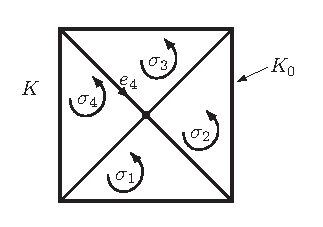
\includegraphics[width=58mm]{figures/1-10-1.pdf}\\图 1.10.1
\end{center}
例 1.6.13 已证明，$K$ 中任意 $1$ 维链 $c$ 都同调于由 $K_0\cup e_4$ 承载的链 $c_3$。若 $c$ 代表相对 $1$ 维闭链，即 $\partial c$ 由 $K_0$ 承载，则 $\partial c_3=\partial c$ 也由 $K_0$ 承载。所以 $c_3$ 在 $e_4$ 上的值必须为零，即 $c_3$ 实际上由 $K_0$ 承载。因此 $H_1(K,K_0)=0$。将此计算与例 1.10.2 比较，使尚待证明的“相对同调群是拓扑不变量”这一断言更为可信。

\entry{例}{1.10.5}设 $K$ 为图 1.10.2 的复形，其底空间称为\textbf{环带}（annulus）。令 $K_0$ 为底空间等于 $K$ 的内外两条边界之并的一维复形。计算 $K$ 模 $K_0$ 的同调。
\begin{center}
\begin{minipage}{.47\textwidth}\centering
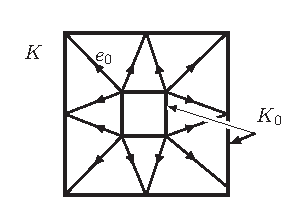
\includegraphics[width=56mm]{figures/1-10-2.pdf}\\图 1.10.2
\end{minipage}\hfill
\begin{minipage}{.47\textwidth}\centering
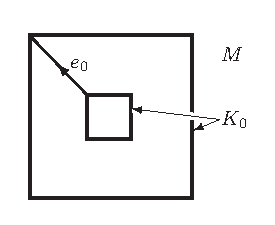
\includegraphics[width=51mm]{figures/1-10-3.pdf}\\图 1.10.3
\end{minipage}
\end{center}
首先，$H_0(K,K_0)=0$，因为零维相对链群本身就为零。计算 $H_1,H_2$ 之前，先验证三个事实：
\begin{enumerate}[label=(\roman*)]
\item 若 $c$ 为 $K$ 的 $1$ 维链，则它同调于由图 1.10.3 中子复形 $M$ 承载的某条 $1$ 维链。
\item 给 $K$ 的所有 $2$ 维单形逆时针定向。若 $d$ 为 $K$ 的任意 $2$ 维链，且 $\partial d$ 由 $M$ 承载，则 $d=m\gamma$，其中 $\gamma$ 为所有定向 $2$ 维单形的和。
\item $\partial\gamma$ 由 $K_0$ 承载。
\end{enumerate}
令 $e_0$ 为图 1.10.2 中的定向 $1$ 维单形。因为 $\partial e_0$ 位于 $K_0$，所以 $e_0$ 代表相对 $1$ 维闭链。由 (i)，任意相对 $1$ 维闭链都相对同调于 $\{e_0\}$ 的某个整数倍。而这样的非零相对闭链不会是相对边界。事实上，若对于 $K$ 的某条 $2$ 维链 $d$，$ne_0-\partial d$ 由 $K_0$ 承载，则 $\partial d$ 由 $M$ 承载，由 (ii) 得 $d=m\gamma$。再由 (iii)，$\partial d=m\partial\gamma$ 由 $K_0$ 承载，所以 $n=0$。因此
\[
H_1(K,K_0)\cong\Z,
\]
相对闭链 $e_0$ 代表一个生成元。利用 (ii)、(iii) 作类似论证，可得 $H_2(K,K_0)\cong\Z$，相对闭链 $\gamma$ 代表一个生成元。

\sourcepage{59--60}
学生常把 $H_p(K,K_0)$ 理解为：将 $|K_0|$ 压缩为一点 $p$ 而得商空间 $X=|K|/|K_0|$ 后，所得空间模该点的同调。若 $X$ 同胚于多面体，因而其单纯同调有定义，这种理解确实正确，但证明并不容易，见引理 8.10.1 及第 4.13 节习题。

粗略地说，$H_p(K,K_0)$ 只依赖于 $K$ 中位于 $K_0$ 之外或其边界上的部分，而忽略 $K_0$ 内部的部分。下面正式表述这个事实。

\entry{定理}{1.10.6（切除定理）}设 $K$ 为复形，$K_0$ 为子复形。设 $U$ 是包含在 $|K_0|$ 中的开集，且 $|K|\setminus U$ 是 $K$ 的某个子复形 $L$ 的多胞体。令 $L_0$ 为多胞体等于 $|K_0|\setminus U$ 的子复形。则包含映射诱导同构
\[
H_p(L,L_0)\cong H_p(K,K_0).
\]
可将 $(|L|,|L_0|)$ 视为从 $|K|,|K_0|$ 中切除开集 $U$ 而得，见图 1.10.4。
\begin{center}
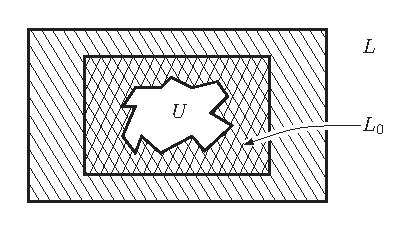
\includegraphics[width=73mm]{figures/1-10-4.pdf}\\图 1.10.4
\end{center}
\noindent\textbf{证明：}考虑复合映射
\[
\varphi:C_p(L)\longrightarrow C_p(K)\longrightarrow C_p(K)/C_p(K_0),
\]
即先包含再投影。$\varphi$ 为满射，因为商群的一组基由所有不属于 $K_0$ 的 $\sigma_i$ 的陪集 $\{\sigma_i\}$ 组成，而 $L$ 包含所有这些单形。$\varphi$ 的核恰为 $C_p(L_0)$。所以对所有 $p$，它诱导同构
\[
C_p(L)/C_p(L_0)\cong C_p(K)/C_p(K_0).
\]
边界算子在此同构下保持不变，故 $H_p(L,L_0)\cong H_p(K,K_0)$。\hfill$\square$

这个初等事实有一些有用的推论，后面将讨论。

\subsection*{习题}
\begin{enumerate}
\item 设 $K$ 为图 1.10.2 的复形，$K_1$ 为其外边界。计算 $H_i(K)$ 与 $H_i(K,K_1)$。
\item 设 $K$ 的底空间为 Möbius 带，$K_0$ 为其边界。计算 $H_i(K)$ 与 $H_i(K,K_1)$。\translatornote{本题原文后一个群写作 $H_i(K,K_1)$，但只定义了 $K_0$；应为 $H_i(K,K_0)$。}［提示：见例 1.4.6，此时边界由线段 $ab,bc,cd,de,ef,fa$ 组成。］
\item 证明：若 $K$ 为复形，$v$ 为其顶点，则对所有 $i$ 有 $H_i(K,v)\cong\widetilde H_i(K)$。［提示：$i=1$ 时需要小心。］
\item 描述一般情况下的 $H_0(K,K_0)$。
\item 用通常的带标记矩形表示环面 $|K|$，令 $K_0$ 为矩形上边所表示的子复形。计算 $H_i(K,K_0)$。［见图 1.7.4，$|K_0|$ 是线段 $ab,bc,ca$ 的并。］
\item 设 $K$ 为二维复形，$\sigma$ 为其一个 $2$ 维单形，$K_0$ 为底空间等于 $|K|\setminus\Int\sigma$ 的子复形。计算 $H_i(K,K_0)$。
\end{enumerate}

\section{\texorpdfstring{$*$}{*}任意系数同调}
\sourcepage{61--62}
这里还要提到另一种同调，虽然要到第六章才详细研究它。这种同调通过引入任意阿贝尔群作为系数群而产生。

设 $G$ 为阿贝尔群，$K$ 为单纯复形。$K$ 的\textbf{以 $G$ 为系数的 $p$ 维链}，是从 $K$ 的定向 $p$ 维单形集到 $G$ 的函数 $c_p$，它除在有限多个单形上外都为零，并且当 $\sigma',\sigma$ 为同一单形的相反定向时，满足 $c_p(\sigma')=-c_p(\sigma)$。通过逐点相加定义加法，所得群记为 $C_p(K;G)$。

若 $\sigma$ 是定向单形，$g\in G$，用 $g\sigma$ 表示如下初等链：在 $\sigma$ 上取值 $g$，在其相反定向上取值 $-g$，在其他所有定向单形上取值 $0$。依此记号，$g(-\sigma)=(-g)\sigma$，其中 $-\sigma$ 仍表示相反定向。给 $K$ 的所有 $p$ 维单形定向后，每条链都能唯一写成初等链的有限和 $c_p=\sum g_i\sigma_i$。因此，$C_p(K;G)$ 是若干与 $G$ 同构的子群的直和，每个 $p$ 维单形对应一个直和项。

边界算子 $\partial:C_p(K;G)\to C_{p-1}(K;G)$ 由公式
\[
\partial(g\sigma)=g(\partial\sigma)
\]
定义，其中 $\partial\sigma$ 是先前定义的普通边界。仍有 $\partial\circ\partial=0$。定义 $Z_p(K;G)$ 为该同态的核，$B_{p-1}(K;G)$ 为其像，并定义
\[
H_p(K;G)=Z_p(K;G)/B_p(K;G).
\]
这些群分别称为 $K$ 的\textbf{以 $G$ 为系数的闭链群、边界链群和同调群}。

当然，也可以研究以 $G$ 为系数的相对同调，具体细节是清楚的，相应的群记为 $H_p(K,K_0;G)$。

接下来一段时间不会深入研究一般系数同调，但应当及早知道它的存在，因为它有时很有用。

\entry{例}{1.11.1}经常用作系数群的一个群是模 $2$ 整数群 $\Z/2$。用它计算环面与 Klein 瓶的同调。第 1.7 节关于环面的论证基本不变，得到
\[
H_1(T;\Z/2)\cong\Z/2\oplus\Z/2,\qquad H_2(T;\Z/2)\cong\Z/2.
\]
对于 Klein 瓶 $S$，论证仍适用，但有一些变化，结果为
\[
H_1(S;\Z/2)\cong\Z/2\oplus\Z/2,\qquad H_2(S;\Z/2)\cong\Z/2.
\]
以 $\Z/2$ 为系数时，由 $S$ 的所有 $2$ 维单形组成的基本 $2$ 维链 $\gamma$ 的边界为零，因为在 $\Z/2$ 中，$2=1+1=0$。

注意，$\Z/2$ 系数同调不足以区分 $T$ 和 $S$。

\entry{例}{1.11.2}用有理数 $\mathbb Q$ 作系数计算环面和 Klein 瓶的同调。前面的论证仍适用，但最终结果不同。对于环面，
\[
H_1(T;\mathbb Q)\cong\mathbb Q\oplus\mathbb Q,\qquad H_2(T;\mathbb Q)\cong\mathbb Q.
\]
对于 Klein 瓶，
\[
H_1(S;\mathbb Q)\cong\mathbb Q,\qquad H_2(S;\mathbb Q)=0.
\]
以 $\mathbb Q$ 为系数时，闭链 $z_1$ 是链 $\tfrac12\gamma$ 的边界。

\subsection*{习题}
\begin{enumerate}
\item 分别用 $\Z/2$ 和 $\mathbb Q$ 作系数，计算 $P^2$ 的同调。
\item 证明 $\mathbb Q$ 系数同调足以区分 $S^2$、连通和 $P^2\mathbin{\#}\cdots\mathbin{\#}P^2$，以及 $T\mathbin{\#}\cdots\mathbin{\#}T$。
\item 分别用 $\Z/3$ 和 $\Z/4$ 作系数，计算 Klein 瓶 $S$ 的同调。
\item 分别用 $\Z/n$ 和 $\mathbb Q$ 作系数，计算 $k$ 重笨帽空间的同调，见第 1.7 节习题 6。
\item 设 $(K,K_0)$ 为 Möbius 带及其边界组成的偶。计算 $H_i(K,K_0;\Z/2)$ 与 $H_i(K,K_0;\mathbb Q)$，见第 1.10 节习题 2。
\end{enumerate}

\section{\texorpdfstring{$*$}{*}同调群的可计算性}
\sourcepage{63--64}
我们已计算过球面、环面和 Klein 瓶等熟悉空间的同调群。现在要问：一般情况下，同调群是否确实能够计算？对于有限复形，答案是肯定的。本节给出进行这种计算的明确算法。

首先证明一个基本定理，给出有限生成自由阿贝尔群之间同态的一种“标准形”，其证明是构造性的。第一个推论是前面陈述的关于自由阿贝尔群子群的定理 1.5.2；第二个推论是自由链复形的标准基定理；第三个推论给出所需的有限复形同调群计算算法。

先证明两个你可能已熟悉的引理。

\entry{引理}{1.12.1}设 $A$ 为秩为 $n$ 的自由阿贝尔群。若 $B$ 为 $A$ 的子群，则 $B$ 为秩 $r\leq n$ 的自由阿贝尔群。

\noindent\textbf{证明：}不妨设 $B$ 为 $n$ 重直积 $\Z^n=\Z\times\cdots\times\Z$ 的子群。如下构造 $B$ 的基。

以 $\pi_i:\Z^n\to\Z$ 表示第 $i$ 坐标投影。对于每个 $m\leq n$，定义
\[
B_m=B\cap(\Z^m\times0).
\]
也就是说，$B_m$ 由所有对 $i>m$ 满足 $\pi_i(x)=0$ 的 $x\in B$ 组成。特别地，$B_n=B$。同态 $\pi_m:B_m\to\Z$ 的像是 $\Z$ 的子群。若此子群平凡，令 $x_m=0$；否则选取 $x_m\in B_m$，使 $\pi_m(x_m)$ 生成该子群。断言：$\{x_1,\ldots,x_n\}$ 中的非零元素构成 $B$ 的一组基。

先证明，对每个 $m$，$x_1,\ldots,x_m$ 生成 $B_m$，从而全部 $x_i$ 生成 $B$。对 $m$ 归纳。$x_1$ 生成 $B_1$ 是显然的：若 $d=\pi_1(x_1)$，则 $x_1=(d,0,\ldots,0)$，而 $B_1$ 恰由其所有整数倍组成。即使 $x_1=0,d=0$，仍如此。

设 $x_1,\ldots,x_{m-1}$ 生成 $B_{m-1}$，取 $x\in B_m$。对某个整数 $k$，有 $\pi_m(x)=k\pi_m(x_m)$，所以 $\pi_m(x-kx_m)=0$，即 $x-kx_m\in B_{m-1}$。由归纳假设，
\[
x-kx_m=k_1x_1+\cdots+k_{m-1}x_{m-1},
\]
故 $x_1,\ldots,x_m$ 生成 $B_m$。

其次，对每个 $m$，证明 $\{x_1,\ldots,x_m\}$ 中非零元素的独立性。仍用归纳，$m=1$ 时平凡。设 $m-1$ 时成立。若
\[
\lambda_1x_1+\cdots+\lambda_mx_m=0,
\]
只需证明对每个 $x_i\ne0$ 都有 $\lambda_i=0$。作用 $\pi_m$ 得 $\lambda_m\pi_m(x_m)=0$。因此要么 $\lambda_m=0$，要么 $x_m=0$：若 $\lambda_m\ne0$，则 $\pi_m(x_m)=0$，从而子群 $\pi_m(B_m)$ 平凡，依定义 $x_m=0$。所以
\[
\lambda_m=0\quad\text{若 }x_m\ne0,\qquad
\lambda_1x_1+\cdots+\lambda_{m-1}x_{m-1}=0.
\]
再用归纳假设，即得对 $i<m$，只要 $x_i\ne0$ 就有 $\lambda_i=0$。\hfill$\square$

为后文所用，将此结果推广到任意自由阿贝尔群。

\entry{引理}{1.12.2}若 $A$ 为自由阿贝尔群，则其任意子群 $B$ 都自由。

\noindent\textbf{证明：}上面对有限情形的证明可推广到 $A$ 有无限基的情形。利用良序定理，它等价于选择公理，用具有最大元素的良序集 $J$ 给 $A$ 的基编号。

不妨设 $A$ 等于若干 $\Z$ 的副本的直和，即 $\Z^J$ 中所有只有有限多个非零坐标的元组 $(n_\alpha)_{\alpha\in J}$ 组成的子群。之后的方法与前面一样；由于这个过程可能不熟悉，给出细节。

设 $B$ 为 $A$ 的子群。对于 $\beta\in J$，令 $B_\beta$ 由所有当 $\alpha>\beta$ 时满足 $\pi_\alpha(x)=0$ 的 $x\in B$ 组成。考察 $\Z$ 的子群 $\pi_\beta(B_\beta)$：若其平凡，令 $x_\beta=0$；否则选取 $x_\beta\in B_\beta$，使 $\pi_\beta(x_\beta)$ 生成此子群。

\sourcepage{65}
先证明 $\{x_\alpha:\alpha\leq\beta\}$ 生成 $B_\beta$。若 $\beta$ 是 $J$ 的最小元素，这显然成立。一般地，用超限归纳。给定 $x\in B_\beta$，对某个整数 $k$，有 $\pi_\beta(x)=k\pi_\beta(x_\beta)$，故 $\pi_\beta(x-kx_\beta)=0$。考虑使 $\pi_\alpha(x-kx_\beta)\ne0$ 的所有指标 $\alpha$。若没有，则 $x=kx_\beta$，证明结束。否则，由 $x,x_\beta\in B_\beta$ 知，这些指标都小于 $\beta$；且它们只有有限多个，所以存在最大值 $\gamma<\beta$。于是 $x-kx_\beta\in B_\gamma$，由归纳假设，它可写成各 $x_\alpha$（$\alpha\leq\gamma$）的线性组合。

再证明 $\{x_\alpha:\alpha\leq\beta\}$ 中非零元素的独立性。$\beta$ 最小时平凡。一般地，设
\[
\lambda_{\alpha_1}x_{\alpha_1}+\cdots+\lambda_{\alpha_k}x_{\alpha_k}
+\lambda_\beta x_\beta=0,\qquad \alpha_i<\beta.
\]
作用 $\pi_\beta$ 得 $\lambda_\beta\pi_\beta(x_\beta)=0$。与前面一样，要么 $\lambda_\beta=0$，要么 $x_\beta=0$。所以当 $x_\beta\ne0$ 时，$\lambda_\beta=0$，并有
\[
\lambda_{\alpha_1}x_{\alpha_1}+\cdots+\lambda_{\alpha_k}x_{\alpha_k}=0.
\]
归纳假设说明，只要 $x_{\alpha_i}\ne0$，就有 $\lambda_{\alpha_i}=0$。\hfill$\square$

现在证明基本定理，先作一个定义。

\entry{定义}{1.12.3}设自由阿贝尔群 $G,G'$ 分别有基 $a_1,\ldots,a_n$ 与 $a'_1,\ldots,a'_m$。若 $f:G\to G'$ 为同态，则对于唯一确定的整数 $\lambda_{ij}$，有
\[
f(a_j)=\sum_{i=1}^m\lambda_{ij}a'_i.
\]
矩阵 $(\lambda_{ij})$ 称为 $f$ 关于给定基的\textbf{矩阵}。

\entry{定理}{1.12.4}设 $G,G'$ 分别为秩 $n,m$ 的自由阿贝尔群，$f:G\to G'$ 为同态。存在它们的基，使 $f$ 关于这些基的矩阵具有形式
\[
B=\begin{pmatrix}
\operatorname{diag}(b_1,\ldots,b_\ell)&0\\0&0
\end{pmatrix},\qquad b_i\geq1,\quad b_1\mid b_2\mid\cdots\mid b_\ell.
\]
此矩阵由 $f$ 唯一确定，尽管相应的基并不唯一。称它为 $f$ 的矩阵的\textbf{标准形}（normal form）。

\sourcepage{66--67}
\noindent\textbf{证明：}先任意为 $G,G'$ 选择基，令 $A$ 为 $f$ 关于它们的矩阵。下面给出修改基的过程，使矩阵化为定理的标准形，从而证明定理。

\entry{定义}{1.12.5}整数矩阵 $A$ 的\textbf{初等行变换}为：
\begin{enumerate}[label=(\arabic*)]
\item 交换第 $i$ 行与第 $k$ 行。
\item 第 $i$ 行乘以 $-1$。
\item 用“第 $i$ 行 $+q$ 倍第 $k$ 行”替换第 $i$ 行，其中 $q$ 为整数，$k\ne i$。
\end{enumerate}
每种变换都对应 $G'$ 中的基变换：第一种交换 $a'_i,a'_k$；第二种将 $a'_i$ 换为 $-a'_i$；第三种将 $a'_k$ 换为 $a'_k-qa'_i$，容易验证。还有三种类似的\textbf{初等列变换}，对应 $G$ 中的基变换。

下面说明如何用这六种初等变换，把任意整数矩阵 $A$ 化为所需标准形。设 $A$ 不是零矩阵，否则平凡。开始介绍算法之前，先注意：若整数 $c$ 整除 $A$ 的每个元素，且 $B$ 由 $A$ 经过任意一种初等变换得到，则 $c$ 也整除 $B$ 的每个元素。

\subsection*{化简算法}
算法从给定的非零整数矩阵 $A=(a_{ij})$ 出发，使用初等变换产生定理 1.12.4 的化简形式。

\entry{定义}{1.12.6}对非零整数矩阵 $A=(a_{ij})$，令 $\alpha(A)$ 为各数 $|a_{ij}|$ 中最小的非零值。若 $|a_{ij}|=\alpha(A)$，则称 $a_{ij}$ 为 $A$ 的一个\textbf{最小元素}。

\entry{引理}{1.12.7}设 $A$ 为非零整数矩阵。$\alpha(A)$ 不能整除 $A$ 的某个元素，当且仅当可以对 $A$ 施行初等变换，使 $\alpha$ 的值减小。

\noindent\textbf{证明：}设最小元素 $a_{ij}$ 不能整除 $A$ 的某个元素。若它不能整除同列的元素 $a_{kj}$，用 Euclid 除法引理写成
\[
a_{kj}=qa_{ij}+r,\qquad0<|r|<|a_{ij}|.
\]
这里不必限制符号，$q,r$ 均可正可负。将第 $k$ 行换为“第 $k$ 行减去 $q$ 倍第 $i$ 行”，\translatornote{原文将行操作印为“第 $i$ 行减去 $q$ 倍第 $k$ 行”，但紧接着计算的是 $a_{kj}-qa_{ij}=r$，应为此处的操作。}则新矩阵第 $k$ 行第 $j$ 列的元素为 $r$，所以新矩阵的 $\alpha$ 至多为 $|r|$，小于 $\alpha(A)$。若 $a_{ij}$ 不能整除同行的某个元素，也类似。

最后，设 $a_{ij}$ 整除其所在行、列的每个元素，但不能整除某个 $a_{st}$，其中 $s\ne i,t\ne j$。考察四个位置
\[
\begin{matrix}a_{ij}&\cdots&a_{it}\\\vdots&&\vdots\\a_{sj}&\cdots&a_{st}\end{matrix}.
\]
由于 $a_{ij}\mid a_{sj}$，可用初等行变换使这些位置成为
\[
\begin{matrix}a_{ij}&\cdots&a_{it}\\\vdots&&\vdots\\0&\cdots&a_{st}+\ell a_{it}\end{matrix}.
\]
再将第 $i$ 行换为第 $i$ 行与第 $s$ 行之和，得到
\[
\begin{matrix}a_{ij}&\cdots&a_{st}+(\ell+1)a_{it}\\\vdots&&\vdots\\0&\cdots&a_{st}+\ell a_{it}\end{matrix}.
\]
因为 $a_{ij}\mid a_{it}$，它不能整除 $a_{st}+(\ell+1)a_{it}$，于是回到不能整除同行某元素的情形。

反方向，若 $\alpha(A)$ 整除 $A$ 的每个元素，则初等变换得到的任何矩阵 $B$ 仍非零，且 $\alpha(A)$ 仍整除其每个元素。选择任意非零元素 $b_{ij}$，则 $|b_{ij}|\geq\alpha(A)$。\hfill$\square$

\sourcepage{68}
\noindent\textbf{算法的主要步骤。}设给定分块矩阵
\[
\begin{pmatrix}\operatorname{diag}(b_1,\ldots,b_k)&0\\0&A\end{pmatrix},\tag{$*$}
\]
满足：
\begin{enumerate}[label=(\arabic*)]
\item 正整数集 $\{b_1,\ldots,b_k\}$ 可以为空，且 $b_1\mid\cdots\mid b_k$。
\item $A$ 为非零整数矩阵，$b_k$ 整除其所有元素。
\end{enumerate}
对 $A$ 作初等变换，相当于对大矩阵 $(*)$ 的相应行、列作同样变换。

令 $A_0=A$。由引理 1.12.7，若 $\alpha(A_0)$ 不整除 $A_0$ 的每个元素，则可施行初等变换，得到满足 $\alpha(A_1)<\alpha(A_0)$ 的矩阵 $A_1$。重复这个过程，不超过 $\alpha(A_0)$ 次，就得到 $\alpha(A_r)$ 整除每个元素的矩阵 $A_r$。继续变换它，但为方便仍记作 $A_r$。

把一个最小元素移至左上角，并使其为正。因为它整除同行同列的所有元素，可以用初等变换把同行同列的其他元素都化为零。此过程结束后，左上角元素仍整除矩阵的每个元素，特别是整除删去第一行、第一列后得到的子矩阵 $A'$ 的所有元素。以 $b_{k+1}$ 表示此左上角元素。

于是，经过初等变换，$(*)$ 化为
\[
\begin{pmatrix}
\operatorname{diag}(b_1,\ldots,b_k)&0&0\\
0&b_{k+1}&0\\0&0&A'
\end{pmatrix},
\]
其中 $b_i\geq1$，$b_1\mid\cdots\mid b_k\mid b_{k+1}$，$b_{k+1}$ 整除 $A'$ 的每个元素，而且 $A'$ 比 $A$ 少一行、一列。

\noindent\textbf{终止条件。}若 $A'$ 全为零或为空，就得到所需标准形；否则重复主要步骤。

\noindent\textbf{定理 1.12.4 证明的完成。}由第 1.5 节习题 4，各数 $b_1,\ldots,b_\ell$ 由同态 $f$ 唯一确定。事实上，非零元素个数 $\ell$ 正是自由阿贝尔群 $f(G)\subset G'$ 的秩，而大于 $1$ 的那些 $b_i$ 正是商群 $G'/f(G)$ 的挠系数 $t_1,\ldots,t_k$。\translatornote{原文称 $G'/f(G)$ 为“挠群”，它一般还可有自由部分；所需的是其挠系数。}\hfill$\square$

\sourcepage{69}
\subsection*{化简算法的应用}
现在证明第 1.5 节陈述的自由阿贝尔群子群基本定理。

\noindent\textbf{定理 1.5.2 的证明：}给定秩为 $n$ 的自由阿贝尔群 $F$，由引理 1.12.1，任意子群 $R$ 都自由，秩 $r\leq n$。考察包含同态 $j:R\to F$，为 $R$ 选择基 $a_1,\ldots,a_r$，为 $F$ 选择基 $e_1,\ldots,e_n$，使 $j$ 的矩阵具有定理 1.12.4 的标准形。由于 $j$ 为单同态，这个标准形没有零列。所以对 $i=1,\ldots,r$，$j(a_i)=b_i e_i$，其中 $b_i\geq1$ 且 $b_1\mid\cdots\mid b_r$。因为 $j(a_i)=a_i$，故 $b_1e_1,\ldots,b_re_r$ 为 $R$ 的一组基。\hfill$\square$

现在引入链复形，并证明自由链复形的标准基定理。

\entry{定义}{1.12.8}\textbf{链复形}（chain complex）$\mathcal C$ 是由整数编号的一列阿贝尔群及同态
\[
\cdots\longrightarrow C_{p+1}\xrightarrow{\partial_{p+1}}C_p
\xrightarrow{\partial_p}C_{p-1}\longrightarrow\cdots,
\]
满足对所有 $p$，有 $\partial_p\circ\partial_{p+1}=0$。定义其第 $p$ 同调群为
\[
H_p(\mathcal C)=\ker\partial_p/\operatorname{im}\partial_{p+1}.
\]
若此群有限生成，其 Betti 数和挠系数称为 $\mathcal C$ 的 $p$ 维 Betti 数和挠系数。

\entry{定理}{1.12.9（自由链复形的标准基）}设 $\{C_p,\partial_p\}$ 为链复形，每个 $C_p$ 都为有限秩自由群。对于每个 $p$，存在 $C_p$ 的子群 $U_p,V_p,W_p$，使
\[
C_p=U_p\oplus V_p\oplus W_p,
\]
其中 $\partial_p(U_p)\subset W_{p-1}$，$\partial_p(V_p)=0$，$\partial_p(W_p)=0$。此外，存在 $U_p$ 与 $W_{p-1}$ 的基，使 $\partial_p:U_p\to W_{p-1}$ 的矩阵为
\[
\operatorname{diag}(b_1,\ldots,b_\ell),\qquad
b_i\geq1,\quad b_1\mid\cdots\mid b_\ell.
\]

\sourcepage{70--71}
\noindent\textbf{证明：第一步。}令 $Z_p=\ker\partial_p$，$B_p=\operatorname{im}\partial_{p+1}$。令 $W_p$ 为所有某个非零整数倍属于 $B_p$ 的元素 $c_p\in C_p$ 构成的集合。这是 $C_p$ 的子群，称为\textbf{弱边界群}（group of weak boundaries）。有
\[
B_p\subset W_p\subset Z_p\subset C_p.
\]
第二个包含关系成立，是因为链群无挠：由 $mc_p=\partial_{p+1}d_{p+1}$ 得 $m\partial_pc_p=0$，从而 $\partial_pc_p=0$。\translatornote{原文此处说 $C_p$ 无挠；这一步实际使用的是 $C_{p-1}$ 无挠，而定理的假设保证了这一点。}

考察自然投影 $Z_p\to H_p(\mathcal C)\to H_p(\mathcal C)/T_p(\mathcal C)$，其中 $T_p$ 为挠子群。其核为 $W_p$，所以 $Z_p/W_p\cong H_p/T_p$。后者有限生成且无挠，故自由。若 $c_1+W_p,\ldots,c_k+W_p$ 为 $Z_p/W_p$ 的基，$d_1,\ldots,d_\ell$ 为 $W_p$ 的基，则容易验证 $c_1,\ldots,c_k,d_1,\ldots,d_\ell$ 为 $Z_p$ 的基。因此 $Z_p=V_p\oplus W_p$，其中 $V_p$ 以 $c_1,\ldots,c_k$ 为基。

\textbf{第二步。}选择 $C_p$ 的基 $e_1,\ldots,e_n$ 和 $C_{p-1}$ 的基 $e'_1,\ldots,e'_m$，使 $\partial_p$ 的矩阵为标准形：对 $i\leq\ell$，$\partial_pe_i=b_i e'_i$；对 $i>\ell$，$\partial_pe_i=0$，其中 $b_i\geq1$，$b_1\mid\cdots\mid b_\ell$。则：
\begin{enumerate}[label=(\arabic*)]
\item $e_{\ell+1},\ldots,e_n$ 为 $Z_p$ 的一组基。
\item $e'_1,\ldots,e'_\ell$ 为 $W_{p-1}$ 的一组基。
\item $b_1e'_1,\ldots,b_\ell e'_\ell$ 为 $B_{p-1}$ 的一组基。
\end{enumerate}
证明如下。一般的 $p$ 维链及其边界为
\[
c_p=\sum_{i=1}^n a_i e_i,\qquad
\partial_pc_p=\sum_{i=1}^\ell a_i b_i e'_i.
\]
因为 $b_i\ne0$，此链为闭链，当且仅当 $i=1,\ldots,\ell$ 时 $a_i=0$，这证明了 (1)。任何边界 $\partial_pc_p$ 都位于 $b_1e'_1,\ldots,b_\ell e'_\ell$ 生成的群中，而这些元素独立，证明了 (3)。最后证明 (2)：每个 $e'_i$（$i\leq\ell$）属于 $W_{p-1}$，因为 $b_i e'_i=\partial e_i$。反过来，若
\[
c_{p-1}=\sum_{i=1}^m d_i e'_i\in W_{p-1},
\]
则对于某个 $\lambda\ne0$，有
\[
\lambda c_{p-1}=\partial_pc_p=\sum_{i=1}^\ell a_i b_i e'_i.
\]
比较系数，对 $i>\ell$ 得 $\lambda d_i=0$，故 $d_i=0$。因此 $e'_1,\ldots,e'_\ell$ 为 $W_{p-1}$ 的基。\translatornote{原文在此最后一句将下标印作 $W_{-1}$。}

\textbf{第三步。}选择第二步的基，令 $U_p$ 由 $e_1,\ldots,e_\ell$ 张成，则 $C_p=U_p\oplus Z_p$。按第一步选取 $V_p$，使 $Z_p=V_p\oplus W_p$。于是得到所需分解，且 $\partial_p(V_p)=\partial_p(W_p)=0$。$U_p,W_{p-1}$ 的所需基由第二步得到。\hfill$\square$

注意，$W_p$ 与 $Z_p=V_p\oplus W_p$ 是 $C_p$ 中唯一确定的子群，而 $U_p,V_p$ 并不唯一。

\entry{定理}{1.12.10}有限复形 $K$ 的同调群可以有效计算。

\noindent\textbf{证明：}由前一定理，存在分解 $C_p(K)=U_p\oplus V_p\oplus W_p$，其中 $Z_p=V_p\oplus W_p$ 为闭链群，$W_p$ 为弱边界群。有
\[
H_p(K)=Z_p/B_p\cong V_p\oplus(W_p/B_p)
\cong(Z_p/W_p)\oplus(W_p/B_p).
\]
$Z_p/W_p$ 自由，$W_p/B_p$ 为挠群，所以计算 $H_p(K)$ 归结为计算这两个群。

固定地给 $K$ 的单形定向，为每个链群选择基。边界同态 $\partial_p:C_p(K)\to C_{p-1}(K)$ 关于这些基的矩阵元素均属于 $\{-1,0,1\}$。利用前述算法将它化为标准形。从上个证明第二步的结果可得：
\begin{enumerate}[label=(\arabic*)]
\item $Z_p$ 的秩等于零列的个数。
\item $W_{p-1}$ 的秩等于非零行的个数。
\item $W_{p-1}/B_{p-1}\cong\Z/b_1\oplus\cdots\oplus\Z/b_\ell$。
\end{enumerate}
\sourcepage{72--73}
因此，$\partial_p$ 的矩阵标准形给出 $K$ 的 $p-1$ 维挠系数，即其中大于 $1$ 的元素；它也给出 $Z_p$ 的秩。另一方面，$\partial_{p+1}$ 的标准形给出 $W_p$ 的秩。两个秩之差就是 $Z_p/W_p$ 的秩，即 $K$ 的 $p$ 维 Betti 数。\hfill$\square$

\subsection*{习题}
\begin{enumerate}
\item 证明：若只计算有限复形 $K$ 的 Betti 数，不需要上述化简算法，只需要一个求矩阵秩的算法。具体地，若 $A_p$ 是 $\partial_p:C_p(K)\to C_{p-1}(K)$ 关于某些基的矩阵，则
\[
\beta_p(K)=\operatorname{rank}C_p(K)-\operatorname{rank}A_p-\operatorname{rank}A_{p+1}.
\]
\item 计算图 1.12.1 所示商空间的同调群。［提示：先检查是否所有顶点都被等同。］
\begin{center}
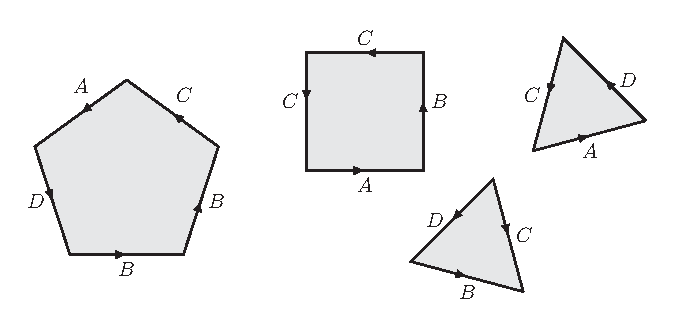
\includegraphics[width=117mm]{figures/1-12-1.pdf}\\图 1.12.1
\end{center}
\item 将下列矩阵化为标准形：
\[
\begin{pmatrix}2&6&4\\4&-7&4\\4&8&4\end{pmatrix}.
\]
\end{enumerate}

\section{单纯映射诱导的同态}
\sourcepage{73--74}
若 $f$ 为从 $|K|$ 到 $|L|$ 的单纯映射，它把 $K$ 的每个 $p$ 维单形 $\sigma_i$ 映到 $L$ 的某个同维或低维单形 $\tau_i$ 上。下面定义 $p$ 维链之间的同态，把定向 $p$ 维单形的形式和 $\sum m_i\sigma_i$ 映到其像的形式和 $\sum m_i\tau_i$，删去后者中所有维数小于 $p$ 的 $\tau_i$。我们将看到，这个映射又诱导同调群之间的同态。

作为一般约定，“$f:K\to L$ 是单纯映射”表示：$f$ 是从 $|K|$ 到 $|L|$ 的连续映射，把 $K$ 的每个单形线性地映到 $L$ 的某个单形上。因此，它把顶点映到顶点，而且等于第 1.3 节所定义的由此顶点映射诱导的单纯映射。

\entry{定义}{1.13.1}设 $f:K\to L$ 为单纯映射。若 $v_0\cdots v_p$ 为 $K$ 的单形，则 $f(v_0),\ldots,f(v_p)$ 张成 $L$ 的单形。通过在定向单形上规定
\[
f_\#([v_0,\ldots,v_p])=
\begin{cases}
[f(v_0),\ldots,f(v_p)],&\text{若各 }f(v_i)\text{ 互异},\\
0,&\text{否则},
\end{cases}
\]
定义同态 $f_\#:C_p(K)\to C_p(L)$。它显然良定义：交换 $[v_0,\ldots,v_p]$ 中两个顶点，等式右边改变符号。在每个维数上各有一个这样的同态，它们组成的族 $\{f_\#\}$ 称为\textbf{单纯映射 $f$ 诱导的链映射}。

严格来说，应以维数下标区分这些同态，将 $p$ 维映射记为 $(f_\#)_p:C_p(K)\to C_p(L)$。通常像边界算子一样省略下标，由上下文说明。同样，为避免记号繁杂，也用 $\partial$ 同时表示 $K$ 与 $L$ 的边界算子；需要区分时可用 $\partial_K,\partial_L$。

\entry{引理}{1.13.2}同态 $f_\#$ 与 $\partial$ 可交换，因此诱导同态 $f_*:H_p(K)\to H_p(L)$。

\noindent\textbf{证明：}需要证明
\[
\partial f_\#([v_0,\ldots,v_p])=f_\#(\partial[v_0,\ldots,v_p]).\tag{$*$}
\]
设 $\tau$ 为 $f(v_0),\ldots,f(v_p)$ 张成的 $L$ 的单形，分情况讨论。

\textbf{情形一：}$\dim\tau=p$。这些像顶点互异，结论立即由 $f_\#$ 与 $\partial$ 的定义得到。

\textbf{情形二：}$\dim\tau\leq p-2$。由于像顶点不全互异，$(*)$ 左边为零。右边也为零，因为无论删去哪个 $f(v_i)$，余下点中至少仍有两个相同。

\textbf{情形三：}$\dim\tau=p-1$。不妨排序使 $f(v_0)=f(v_1)$，而 $f(v_1),\ldots,f(v_p)$ 互异。左边为零。右边许多项对应的像单形维数为 $p-2$，故这些项为零。仅有的两个非零项为
\[
[f(v_1),f(v_2),\ldots,f(v_p)]-[f(v_0),f(v_2),\ldots,f(v_p)],
\]
两者相互抵消，得到所需等式。

$f_\#$ 把闭链映为闭链，因为 $\partial c_p=0$ 蕴含 $\partial f_\#(c_p)=f_\#(\partial c_p)=0$；它也把边界映为边界，因为 $c_p=\partial d_{p+1}$ 蕴含 $f_\#(c_p)=f_\#(\partial d_{p+1})=\partial f_\#(d_{p+1})$。故它诱导同调群同态 $f_*$。\hfill$\square$

\sourcepage{75}
\entry{定理}{1.13.3}
\begin{enumerate}[label=(\alph*)]
\item 若 $i:K\to K$ 为恒等单纯映射，则 $i_*:H_p(K)\to H_p(K)$ 为恒等同态。
\item 若 $f:K\to L$、$g:L\to M$ 为单纯映射，则 $(g\circ f)_*=g_*\circ f_*$，即从 $H_p(K)$ 经 $H_p(L)$ 到 $H_p(M)$ 的复合，等于直接由 $g\circ f$ 诱导的同态。
\end{enumerate}
\noindent\textbf{证明：}由定义立即可验证，$i_*$ 为恒等映射，且 $(g\circ f)_*=g_*\circ f_*$。\hfill$\square$

这个定理表述了诱导同态的所谓“函子性质”。讨论范畴与函子时将正式定义此术语。现在只需指出：算子 $H_p$ 给每个单纯复形指定一个阿贝尔群，算子 $*$ 给每个单纯映射指定相应群之间的同态。因为 (a)、(b) 成立，称 $(H_p,*)$ 为从单纯复形与单纯映射的“范畴”到阿贝尔群与同态的“范畴”的一个“函子”。

\entry{引理}{1.13.4}链映射 $f_\#$ 保持增广映射 $\epsilon$，因此诱导约化同调群之间的同态 $f_*$。

\noindent\textbf{证明：}对 $K$ 的每个顶点 $v$，有 $\epsilon f_\#(v)=1=\epsilon(v)$，故 $\epsilon\circ f_\#=\epsilon$。因此 $f_\#$ 把 $\epsilon_K:C_0(K)\to\Z$ 的核映到 $\epsilon_L:C_0(L)\to\Z$ 的核中，诱导 $f_*:\widetilde H_0(K)\to\widetilde H_0(L)$。\hfill$\square$

\entry{例}{1.13.5}考虑图 1.13.1 的复形 $K,T$，底空间分别为圆周和环面。$H_1(K)\cong\Z$，取图中闭链 $z$ 为生成元。$H_1(T)\cong\Z\oplus\Z$，以
\[
w_1=[A,B]+[B,C]+[C,A],\qquad z_1=[A,D]+[D,E]+[E,A]
\]
的陪集为基。考虑下表指定的三个单纯映射：
\begin{center}
\begin{tabular}{c|ccc}
顶点&$f$&$g$&$h$\\\hline
$a$&$A$&$A$&$A$\\
$b$&$P$&$B$&$I$\\
$c$&$D$&$C$&$J$\\
$d$&$D$&$A$&$G$\\
$e$&$P$&$E$&$G$\\
$p$&$E$&$D$&$A$
\end{tabular}
\end{center}
可以验证，$f_\#(z)$ 同调于 $z_1$，$g_\#(z)=w_1-z_1$，而 $h_\#(z)$ 同调于 $w_1-z_1$。因此 $g_*,h_*$ 在一维同调上相同，在零维同调上也相同。
\begin{center}
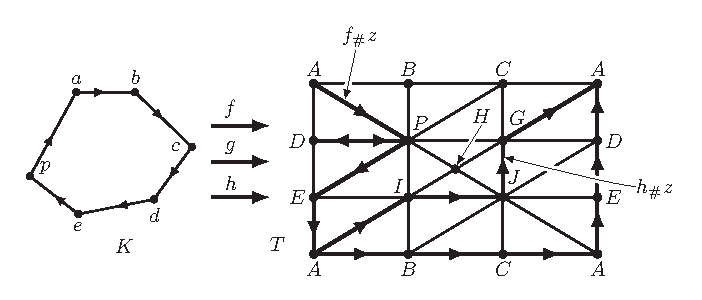
\includegraphics[width=121mm]{figures/1-13-1.pdf}\\图 1.13.1
\end{center}

\sourcepage{76--77}
如前例所示，很不相同的单纯映射也可以诱导同一个同态。因此要问：在什么条件下，两个单纯映射诱导同一个同调群同态？回答这个问题需要一种重要技巧，后文将多次使用，先解释其动机。

给定单纯映射 $f,g:K\to L$，希望找到条件，保证每个闭链 $z\in Z_p(K)$ 的像 $f_\#(z),g_\#(z)$ 同调。换言之，希望有一个通常记作 $D$ 的函数，为每条 $p$ 维闭链 $z$ 指定 $L$ 的一条 $(p+1)$ 维链 $Dz$，使
\[
\partial Dz=g_\#(z)-f_\#(z).
\]
考虑一个能做到这一点的例子。设 $K$ 为三角形区域的边界，$L$ 由图 1.13.2 的三棱柱侧面组成；$f,g$ 分别把 $K$ 映到棱柱的两端。若 $z$ 为图中生成 $H_1(K)$ 的闭链，很容易找到边界为 $g_\#(z)-f_\#(z)$ 的 $2$ 维链 $Dz$：取 $L$ 中所有适当定向的 $2$ 维单形之和即可。
\begin{center}
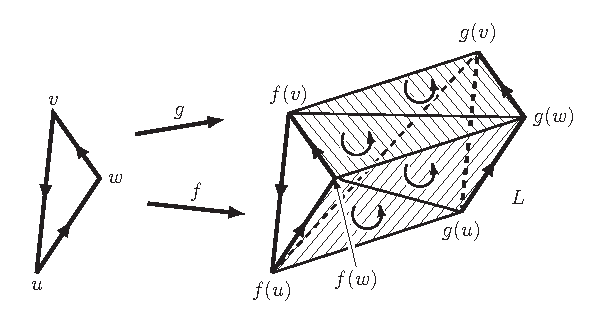
\includegraphics[width=105mm]{figures/1-13-2.pdf}\\图 1.13.2
\end{center}
一般地，只在闭链上定义 $D$ 很不方便，因为需要先计算闭链群。更好的办法是在整个链群上把 $D$ 定义为同态，这样可以逐个单形定义。在本例中如何做呢？给定顶点 $v$，定义 $Dv$ 为从 $f(v)$ 到 $g(v)$ 的边，如图 1.13.3。给定定向 $1$ 维单形 $\sigma$，定义 $D\sigma$ 为图中深色阴影的两个定向单形之和，它们组成棱柱的一个侧面。对其他单形也类似。由于 $z$ 是各定向边之和，$Dz$ 就是 $L$ 的所有定向 $2$ 维单形之和，仍满足所需等式。

对于任意链 $c$，$\partial Dc$ 满足什么公式？由定义即可看出。对定向单形 $\sigma$，由图 1.13.3 验证
\[
\partial D\sigma=g_\#(\sigma)-Dv-f_\#(\sigma)+Dw,
\]
即
\[
\partial(D\sigma)=g_\#(\sigma)-f_\#(\sigma)-D(\partial\sigma).\tag{$**$}
\]
对 $K$ 的其他单形也有相同公式。
\begin{center}
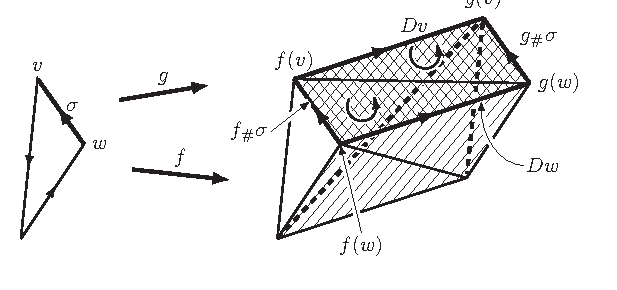
\includegraphics[width=105mm]{figures/1-13-3.pdf}\\图 1.13.3
\end{center}
这表述了同态 $D$ 的关键代数性质，正是我们所寻求的公式，将其纳入定义。

\sourcepage{78--79}
\entry{定义}{1.13.6}设 $f,g:K\to L$ 为单纯映射。若对每个 $p$ 都有同态 $D:C_p(K)\to C_{p+1}(L)$，满足
\[
\partial D+D\partial=g_\#-f_\#,
\]
则称 $D$ 为 $f_\#$ 与 $g_\#$ 之间的\textbf{链同伦}（chain homotopy）。

这里省略了维数下标。写出下标，公式为
\[
\partial_{p+1}D_p+D_{p-1}\partial_p=(g_\#)_p-(f_\#)_p,
\]
其中 $D_p:C_p(K)\to C_{p+1}(L)$，$D_{p-1}:C_{p-1}(K)\to C_p(L)$。这更精确，但记号繁杂，通常仍省略下标。

链同伦的重要性来自下列定理。

\entry{定理}{1.13.7}若 $f_\#$ 与 $g_\#$ 之间存在链同伦，则其诱导同态 $f_*,g_*$ 相等，对约化同调和普通同调都成立。

\noindent\textbf{证明：}若 $z$ 为 $p$ 维闭链，则
\[
g_\#(z)-f_\#(z)=\partial Dz+D\partial z=\partial Dz+0,
\]
所以两者属于同一同调类，即 $g_*(\{z\})=f_*(\{z\})$。\hfill$\square$

我们仍要寻找使 $f_*=g_*$ 的条件；现在已将问题归结为：在什么条件下可以构造 $f_\#,g_\#$ 之间的链同伦？下面给出一组条件。

\entry{定义}{1.13.8}若对 $K$ 的每个单形 $v_0\cdots v_p$，点
\[
f(v_0),\ldots,f(v_p),g(v_0),\ldots,g(v_p)
\]
张成 $L$ 的一个单形 $\tau$，则称单纯映射 $f,g:K\to L$ \textbf{邻接}（contiguous）。依互异点的个数，$\tau$ 的维数可为 $0$ 到 $2p+1$ 中的任一数。

粗略地说，这个条件表示 $f,g$ 相当接近：可以穿过某个可能较大的单形 $\tau$，把 $f(\sigma)$ 移到 $g(\sigma)$，而两者都是 $\tau$ 的面。

\entry{定理}{1.13.9}若 $f,g:K\to L$ 邻接，则 $f_\#,g_\#$ 之间存在链同伦。

\noindent\textbf{证明：}下面是一种标准论证，应当掌握。对于 $K$ 的每个单形 $\sigma=v_0\cdots v_p$，令 $L(\sigma)$ 为由顶点集
\[
\{f(v_0),\ldots,f(v_p),g(v_0),\ldots,g(v_p)\}
\]
张成的单形及其各面构成的子复形。注意：
\begin{enumerate}[label=(\arabic*)]
\item $L(\sigma)$ 非空，且对所有 $i$ 有 $\widetilde H_i(L(\sigma))=0$，见定理 1.9.7。
\item 若 $s$ 为 $\sigma$ 的面，则 $L(s)\subset L(\sigma)$。
\item 对每个定向单形 $\sigma$，链 $f_\#(\sigma),g_\#(\sigma)$ 都由 $L(\sigma)$ 承载。
\end{enumerate}
利用这些事实，对 $p$ 归纳构造 $D:C_p(K)\to C_{p+1}(L)$，使每条 $D\sigma$ 都由 $L(\sigma)$ 承载。

令 $p=0$，取顶点 $v$。因为 $f_\#,g_\#$ 保持增广，
\[
\epsilon(g_\#(v)-f_\#(v))=1-1=0.
\]
因此此差代表 $\widetilde H_0(L(v))$ 的元素。该群为零，可选取由 $L(v)$ 承载的 $1$ 维链 $Dv$，使 $\partial Dv=g_\#(v)-f_\#(v)$。于是 $\partial Dv+D\partial v=g_\#(v)-f_\#(v)$。对每个顶点如此定义 $D$。

现设在小于 $p$ 的维数已定义 $D$，使每个这样的定向单形 $s$ 满足 $Ds$ 由 $L(s)$ 承载，且 $\partial Ds+D\partial s=g_\#(s)-f_\#(s)$。给定定向 $p$ 维单形 $\sigma$，希望定义 $D\sigma$，使其边界等于
\[
c=g_\#(\sigma)-f_\#(\sigma)-D\partial\sigma.
\]
因为 $\partial\sigma$ 为 $p-1$ 维链，$D\partial\sigma$ 已定义，故 $c$ 良定义。它还是闭链：对 $\partial\sigma$ 用归纳假设，并利用 $\partial^2=0$，得
\[
\begin{aligned}
\partial c&=\partial g_\#(\sigma)-\partial f_\#(\sigma)-\partial D(\partial\sigma)\\
&=\partial g_\#(\sigma)-\partial f_\#(\sigma)
-\bigl[g_\#(\partial\sigma)-f_\#(\partial\sigma)-D\partial(\partial\sigma)\bigr]\\
&=\partial g_\#(\sigma)-\partial f_\#(\sigma)-g_\#(\partial\sigma)+f_\#(\partial\sigma)=0.
\end{aligned}
\]
\translatornote{原文展开式中有两处多印 $\partial$，成为 $\partial f_\#(\partial\sigma)$，维数不合；这里按链同伦恒等式写出计算。}
再验证 $c$ 由 $L(\sigma)$ 承载。由 (3)，前两项如此。$\partial\sigma$ 是定向面的和，每个面的像 $Ds$ 由 $L(s)$ 承载，而由 (2)，$L(s)\subset L(\sigma)$，故第三项也如此。

因为 $c$ 是由 $L(\sigma)$ 承载的 $p$ 维闭链，且 $H_p(L(\sigma))=0$，可选取同样由其承载的 $(p+1)$ 维链 $D\sigma$，使
\[
\partial D\sigma=c=g_\#(\sigma)-f_\#(\sigma)-D\partial\sigma.
\]
再定义 $D(-\sigma)=-D(\sigma)$。对每个 $p$ 维单形重复此过程，就得到 $p$ 维上所需的链同伦。定理得证。\hfill$\square$

\sourcepage{80--81}
有些学生对构造 $D$ 时必须作任意选择感到不安，希望有一个确定公式。遗憾的是，没有这样一个简洁公式。根本原因在于，$f_\#,g_\#$ 之间可能有许多链同伦，没有理由偏爱其中一个。

以特例说明。证明第一步中，若 $v$ 为顶点，则 $Dv$ 实际唯一确定：因为它必须由 $L(v)$ 承载，所以
\[
Dv=\begin{cases}0,&f(v)=g(v),\\\lbrack f(v),g(v)\rbrack,&f(v)\ne g(v).\end{cases}
\]
第一种情形 $L(v)$ 为顶点，第二种为一条边及其各面。

但下一步就可能有选择。设 $\sigma=vw$ 为边，$f(v),f(w),g(v),g(w)$ 互异，张成图 1.13.4 的 $3$ 维单形 $\tau$。图中给出了 $Dv,Dw$。如何定义 $D\sigma$？对于边界为图 1.13.5 所示 $g_\#(\sigma)-f_\#(\sigma)-D\partial\sigma$ 的 $2$ 维链，有两个明显选择：按图示定向取 $\tau$ 前面的两个面之和，或适当定向取后面的两个面之和。没有理由偏爱其中之一，只能任意选择。
\begin{center}
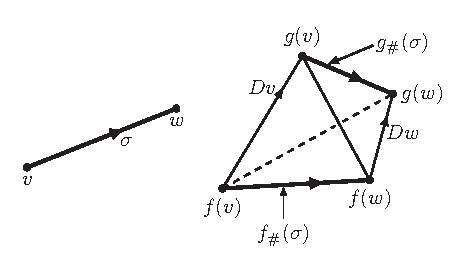
\includegraphics[width=85mm]{figures/1-13-4.pdf}\\图 1.13.4
\medskip

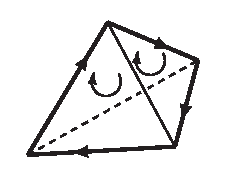
\includegraphics[width=43mm]{figures/1-13-5.pdf}\\图 1.13.5
\end{center}
\subsection*{在相对同调中的应用}
设 $K_0,L_0$ 分别为 $K,L$ 的子复形，单纯映射 $f:K\to L$ 将 $K_0$ 的每个单形映入 $L_0$ 的某个单形。常说“$f:(K,K_0)\to(L,L_0)$ 是单纯映射”。这时 $f_\#$ 将 $C_p(K_0)$ 映入 $C_p(L_0)$，诱导相对链映射
\[
f_\#:C_p(K,K_0)\to C_p(L,L_0).
\]
它与 $\partial$ 可交换，因此诱导同态 $f_*:H_p(K,K_0)\to H_p(L,L_0)$。定理 1.13.3 的函子性质立即推广到相对同调。

\entry{定义}{1.13.10}若 $f,g:(K,K_0)\to(L,L_0)$ 满足：对 $K$ 的每个单形 $\sigma=v_0\cdots v_p$，各点 $f(v_0),\ldots,f(v_p),g(v_0),\ldots,g(v_p)$ 张成 $L$ 的一个单形，且当 $\sigma\in K_0$ 时，它们张成 $L_0$ 的一个单形，则称 $f,g$ \textbf{作为偶的映射邻接}。

\sourcepage{82--84}
\entry{定理}{1.13.11}若 $f,g:(K,K_0)\to(L,L_0)$ 作为偶的映射邻接，则对所有 $p$ 存在同态 $D:C_p(K,K_0)\to C_{p+1}(L,L_0)$，满足 $\partial D+D\partial=g_\#-f_\#$。因此 $f_*,g_*$ 在相对同调群上相等。

\noindent\textbf{证明：}定理 1.13.9 构造的 $D$ 自动将 $C_p(K_0)$ 映入 $C_{p+1}(L_0)$：若 $\sigma\in K_0$，则 $L(\sigma)$ 按定义为 $L_0$ 的子复形，而 $D\sigma$ 由 $L(\sigma)$ 承载。因此 $D$ 诱导了相对链群间所需的同态。\hfill$\square$

\subsection*{习题}
\begin{enumerate}
\item 验证例 1.13.5 中的各项断言。
\item 考虑图 1.13.6 的顶点标记指定的复形 $K$，底空间为环面。虽与前面的复形略有不同，同调计算不变。令 $\gamma$ 为所有逆时针定向 $2$ 维单形之和，则它生成 $H_2(K)$。闭链 $w_1=[a,b]+[b,c]+[c,a]$、$z_1=[a,d]+[d,e]+[e,a]$ 生成 $H_1(K)$。
\begin{enumerate}[label=(\alph*)]
\item 定义 $K$ 到自身的单纯映射 $f,g,h,k$，使其满足下表：
\begin{center}\begin{tabular}{c|cccc}
顶点&$f$&$g$&$h$&$k$\\\hline
$a$&$a$&$a$&$d$&$p$\\
$b$&$d$&$c$&$p$&$q$\\
$c$&$e$&$b$&$q$&$d$\\
$d$&$c$&$d$&$d$&$u$\\
$e$&$b$&$e$&$d$&$b$
\end{tabular}\end{center}
\item 计算 $f_*,g_*,h_*,k_*$ 在同调类 $\{w_1\},\{z_1\},\{\gamma\}$ 上的值。
\end{enumerate}
\begin{center}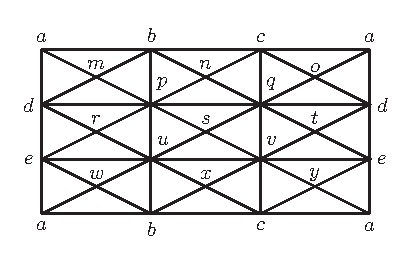
\includegraphics[width=76mm]{figures/1-13-6.pdf}\\图 1.13.6\end{center}
\item 用图 1.13.7 的复形表示 Klein 瓶 $S$，仍令 $w_1=[a,b]+[b,c]+[c,a]$、$z_1=[a,d]+[d,e]+[e,a]$。
\begin{enumerate}[label=(\alph*)]
\item 定义单纯映射 $f:S\to S$，使 $f_*(\{w_1\})=\{z_1\}$。
\item 证明不存在单纯映射 $g:S\to S$，使 $g_*(\{z_1\})=\{w_1\}$。
\end{enumerate}
\begin{center}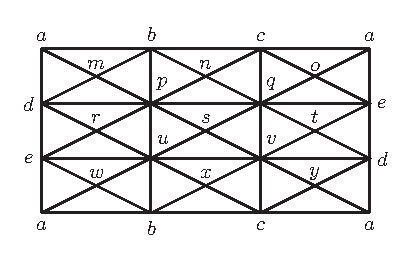
\includegraphics[width=76mm]{figures/1-13-7.pdf}\\图 1.13.7\end{center}
\item 设 $K$ 为习题 2 的环面，$\gamma$ 为其中的 $2$ 维闭链。设 $L$ 由顶点为 $A,B,C,D$ 的 $3$ 维单形的真面组成，令 $\gamma'=\partial[A,B,C,D]$，见图 1.13.8。
\begin{enumerate}[label=(\alph*)]
\item 证明从 $K$ 的顶点集到 $L$ 的顶点集的任意映射，都诱导 $K\to L$ 的单纯映射。
\item 令 $f$ 将 $m,r$ 映到 $A$，$p$ 映到 $B$，$b,u$ 映到 $C$，其他顶点均映到 $D$。用 $\gamma,\gamma'$ 表示诱导同态 $f_*:H_2(K)\to H_2(L)$。
\item 设 $g$ 在除 $r$ 外的顶点上与 $f$ 相同，而 $g(r)=C$，计算 $g_*$。
\item 设 $h$ 在除 $u$ 外的顶点上与 $g$ 相同，而 $h(u)=A$，计算 $h_*$。
\end{enumerate}
\begin{center}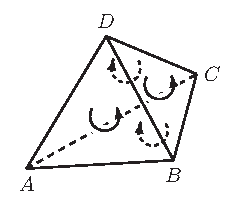
\includegraphics[width=43mm]{figures/1-13-8.pdf}\\图 1.13.8\end{center}
\item 设 $f,g:(K,K_0)\to(L,L_0)$ 为单纯映射。证明：若 $f,g$ 作为 $K\to L$ 的映射邻接，且 $L_0$ 是 $L$ 的满子复形，则它们作为偶的映射邻接，见定义 1.4.11。
\end{enumerate}

\section{链复形与无环载体}
\sourcepage{84--85}
前面在单纯复形的背景下作出的许多定义和构造，也出现在更一般的情形中。这里暂作离题，讨论这种一般背景。后面将多次使用这些结果，部分证明留作习题。

先定义链群的代数类似物，第 1.12 节已提到过它们。

\entry{定义}{1.14.1}\textbf{链复形} $\mathcal C$ 是由整数编号的一族阿贝尔群 $C_p$ 及同态 $\partial_p:C_p\to C_{p-1}$，满足对所有 $p$ 有 $\partial_p\circ\partial_{p+1}=0$。

若 $p<0$ 时 $C_p=0$，则称 $\mathcal C$ 为\textbf{非负链复形}。若每个 $C_p$ 都自由阿贝尔，则称它为\textbf{自由链复形}。群
\[
H_p(\mathcal C)=\ker\partial_p/\operatorname{im}\partial_{p+1}
\]
称为链复形的\textbf{第 $p$ 同调群}。

若 $\mathcal C$ 非负，其一个\textbf{增广}是满足 $\epsilon\circ\partial_1=0$ 的满同态 $\epsilon:C_0\to\Z$。\textbf{增广链复形} $\{\mathcal C,\epsilon\}$ 是在 $\mathcal C$ 的 $-1$ 维添加群 $\Z$，并以 $\epsilon$ 作为零维边界算子而得到的链复形。其同调群称为原链复形相对于增广 $\epsilon$ 的\textbf{约化同调群}，记为 $H_i(\{\mathcal C,\epsilon\})$ 或 $\widetilde H_i(\mathcal C)$。容易得到，当 $p\ne0$ 时 $\widetilde H_p(\mathcal C)=H_p(\mathcal C)$，且
\[
H_0(\mathcal C)\cong\widetilde H_0(\mathcal C)\oplus\Z,
\]
见习题。

若任意链复形 $\mathcal D$ 满足对所有 $i$ 有 $H_i(\mathcal D)=0$，称其\textbf{无环}。特别地，增广链复形 $\{\mathcal C,\epsilon\}$ 无环，表示对所有 $i$，$H_i(\{\mathcal C,\epsilon\})=\widetilde H_i(\mathcal C)=0$；等价地，$H_0(\mathcal C)\cong\Z$，且当 $i\ne0$ 时 $H_i(\mathcal C)=0$。

\entry{定义}{1.14.2}设 $\mathcal C=\{C_p,\partial_p\}$、$\mathcal C'=\{C'_p,\partial'_p\}$ 为链复形。\textbf{链映射} $\varphi:\mathcal C\to\mathcal C'$ 是一族同态 $\varphi_p:C_p\to C'_p$，满足
\[
\partial'_p\circ\varphi_p=\varphi_{p-1}\circ\partial_p
\]
对所有 $p$ 成立。

链映射给出诱导同态 $(\varphi_*)_p:H_p(\mathcal C)\to H_p(\mathcal C')$，并且：
\begin{enumerate}[label=(\alph*)]
\item $\mathcal C$ 的恒等映射 $i$ 为链映射，$(i_*)_p$ 为 $H_p(\mathcal C)$ 的恒等映射。
\item 若 $\varphi:\mathcal C\to\mathcal C'$、$\psi:\mathcal C'\to\mathcal C''$ 为链映射，则 $\psi\circ\varphi$ 也是，且 $(\psi\circ\varphi)_*=\psi_*\circ\varphi_*$。
\end{enumerate}
若两链复形已增广，且 $\epsilon'\circ\varphi_0=\epsilon$，称 $\varphi$ \textbf{保持增广}。将它在 $-1$ 维上扩张为 $\Z$ 的恒等映射，就得到\textbf{增广链复形的链映射}。因此，保持增广的链映射诱导约化同调同态 $\varphi_*:\widetilde H_p(\mathcal C)\to\widetilde H_p(\mathcal C')$。

\entry{例}{1.14.3}第 1.10 节定义的 $\mathcal C(K,K_0)=\{C_p(K,K_0),\partial_p\}$ 称为单纯偶 $(K,K_0)$ 的\textbf{定向链复形}。它自由且非负，但一般没有增广。例如，例 1.10.5 中 $C_0(K,K_0)=0$，不可能满射到 $\Z$。若 $K_0$ 为空，则 $\mathcal C(K,\varnothing)=\mathcal C(K)$ 有标准增广，对每个顶点 $v$ 定义 $\epsilon(v)=1$。

\entry{例}{1.14.4}若 $f:K\to L$ 为单纯映射，则 $f_\#$ 是从 $\mathcal C(K)$ 到 $\mathcal C(L)$ 的保持增广的链映射。一般地，也存在并非由单纯映射诱导的保持增广链映射 $\varphi:\mathcal C(K)\to\mathcal C(L)$。

\entry{定义}{1.14.5}设 $\varphi,\psi:\mathcal C\to\mathcal C'$ 为链映射。从 $\varphi$ 到 $\psi$ 的\textbf{链同伦}是一族同态 $D_p:C_p\to C'_{p+1}$，满足对所有 $p$ 有
\[
\partial'_{p+1}D_p+D_{p-1}\partial_p=\psi_p-\varphi_p.
\]
称 $\varphi,\psi$ \textbf{链同伦}。

\sourcepage{86--87}
今后通常省略边界算子、链映射和链同伦的下标。例如，上式写为更熟悉的 $\partial'D+D\partial=\psi-\varphi$。

\entry{定义}{1.14.6}若链映射 $\varphi:\mathcal C\to\mathcal C'$ 存在链映射 $\varphi':\mathcal C'\to\mathcal C$，使 $\varphi'\circ\varphi$ 与 $\varphi\circ\varphi'$ 分别链同伦于 $\mathcal C$、$\mathcal C'$ 的恒等映射，则称 $\varphi$ 为\textbf{链等价}（chain equivalence），称 $\varphi'$ 为其\textbf{链同伦逆}。

列出链同伦的几个性质，证明留作习题。
\begin{enumerate}[label=(\arabic*)]
\item 链同伦是从 $\mathcal C$ 到 $\mathcal C'$ 的链映射集上的等价关系。
\item 链映射的复合诱导链同伦类之间良定义的复合运算。
\item 若 $\varphi,\psi$ 链同伦，则它们诱导相同的同调同态。
\item 若 $\varphi$ 为链等价，链同伦逆为 $\varphi'$，则 $\varphi_*,(\varphi')_*$ 是互逆的同调同构。
\item 两个链等价的复合仍为链等价。
\end{enumerate}
现在研究增广链复形的特殊情形。

\entry{引理}{1.14.7}设 $\mathcal C,\mathcal C'$ 为非负链复形，$\varphi,\psi:\mathcal C\to\mathcal C'$ 为链映射，$D$ 为两者之间的链同伦。设两复形分别由 $\epsilon,\epsilon'$ 增广。若 $\varphi$ 保持增广，则 $\psi$ 也保持增广。将 $\varphi,\psi$ 在 $-1$ 维扩张为恒等映射，将 $D$ 在 $-1$ 维扩张为零，则 $D$ 是扩张后的链映射之间的链同伦。

\noindent\textbf{证明：}对 $c_0\in C_0$，因为 $\partial c_0=0$，有 $\partial'Dc_0=\psi(c_0)-\varphi(c_0)$。于是
\[
0=\epsilon'(\partial'Dc_0)=\epsilon'\psi(c_0)-\epsilon'\varphi(c_0)
=\epsilon'\psi(c_0)-\epsilon(c_0),
\]
得到所需增广关系。\translatornote{原文此证明将 $\varphi-\psi$ 与前述定义中的 $\psi-\varphi$ 混用；这里统一按定义 1.14.5 的方向书写。}
在增广后的零维上，因为 $D\epsilon(c_0)=0$，有 $D\epsilon(c_0)+\partial'D(c_0)=\psi(c_0)-\varphi(c_0)$。在 $-1$ 维上，$\epsilon'(D(1))=\psi(1)-\varphi(1)$，因为两边均为零。因此扩张后的 $D$ 仍为链同伦。\hfill$\square$

\entry{引理}{1.14.8}设 $\mathcal C,\mathcal C'$ 为分别由 $\epsilon,\epsilon'$ 增广的非负链复形，$\varphi:\mathcal C\to\mathcal C'$ 为链等价，链同伦逆为 $\varphi'$。若 $\varphi$ 保持增广，则 $\varphi'$ 也保持增广。作为增广链复形的映射，两者仍为链同伦逆，因此诱导约化同调上的互逆同构。

\noindent\textbf{证明：}取 $\varphi\circ\varphi'$ 与恒等映射之间的链同伦 $D'$，方向取为
\[
\partial'D'c'_0=\varphi\varphi'(c'_0)-c'_0.
\]
因此
\[
0=\epsilon'(\partial'D'c'_0)=\epsilon'\varphi\varphi'(c'_0)-\epsilon'(c'_0)
=\epsilon\varphi'(c'_0)-\epsilon'(c'_0).
\]
故 $\varphi'$ 保持增广，其余由引理 1.14.7 得到。\hfill$\square$

这些定义建立了一般代数框架，定向单纯链群只是其中的特例。现在把上一节构造链同伦的方法放入此框架。作为动机，先考察链映射任意、链群仍为熟悉的定向单纯链群的情形，再讨论一般链复形。

\entry{定义}{1.14.9}从单纯复形 $K$ 到 $L$ 的\textbf{无环载体}（acyclic carrier）是函数 $\Phi$，为 $K$ 的每个单形 $\sigma$ 指定 $L$ 的子复形 $\Phi(\sigma)$，满足：
\begin{enumerate}[label=(\arabic*)]
\item $\Phi(\sigma)$ 非空且无环。
\item 若 $s$ 为 $\sigma$ 的面，则 $\Phi(s)\subset\Phi(\sigma)$。
\end{enumerate}
若同态 $f:C_p(K)\to C_q(L)$ 对每个定向 $p$ 维单形 $\sigma$，使链 $f(\sigma)$ 由 $\Phi(\sigma)$ 承载，则称 $f$ \textbf{由 $\Phi$ 承载}。

\entry{定理}{1.14.10（无环载体定理，几何形式）}设 $\Phi$ 为从 $K$ 到 $L$ 的无环载体。
\begin{enumerate}[label=(\alph*)]
\item 若 $\varphi,\psi:\mathcal C(K)\to\mathcal C(L)$ 为两个由 $\Phi$ 承载的保持增广链映射，则存在从 $\varphi$ 到 $\psi$ 的、也由 $\Phi$ 承载的链同伦 $D$。
\item 存在由 $\Phi$ 承载的保持增广链映射 $\mathcal C(K)\to\mathcal C(L)$。
\end{enumerate}

\sourcepage{88}
\noindent\textbf{证明：}(a) 直接仿照定理 1.13.9 的证明，将所有子复形 $L(\sigma)$ 换成 $\Phi(\sigma)$ 即可。

为证 (b)，对 $K$ 的每个顶点 $v$，定义 $\varphi(v)$ 为 $\Phi(v)$ 中满足 $\epsilon(c)=1$ 的某条 $0$ 维链 $c$。因为 $\Phi(v)$ 非空，其零维链群的增广满射到 $\Z$，所以可作此选择；事实上，只需取 $\Phi(v)$ 的某个顶点。于是 $\varphi$ 保持增广，并有 $\partial\varphi(v)=0=\varphi(\partial v)$。

设 $\sigma=[v,w]$ 是定向边。因为 $\varphi$ 已在零维定义，$c=\varphi(\partial\sigma)$ 良定义。它由 $\Phi(\sigma)$ 承载：其两项分别由 $\Phi(v),\Phi(w)$ 承载，后两者由 (2) 都包含于 $\Phi(\sigma)$。此外，$\epsilon(c)=\epsilon\varphi(\partial\sigma)=\epsilon(\partial\sigma)=0$，因为 $\varphi$ 保持增广。所以 $c$ 代表 $\widetilde H_0(\Phi(\sigma))$ 的元素。由 (1)，此群为零，故可选择由 $\Phi(\sigma)$ 承载、边界为 $c$ 的 $1$ 维链，记为 $\varphi(\sigma)$。于是 $\partial\varphi(\sigma)=c=\varphi(\partial\sigma)$。

作归纳，设 $p>1$，对 $\dim s<p$ 已定义 $\varphi(s)$，并满足 $\partial\varphi(s)=\varphi\partial(s)$。\translatornote{原文这里的等号误印为减号。}给定定向 $p$ 维单形 $\sigma$，链 $c=\varphi(\partial\sigma)$ 是良定义的 $p-1$ 维链。它由 $\Phi(\sigma)$ 承载，因为各面 $s_i$ 的 $\Phi(s_i)$ 都包含于 $\Phi(\sigma)$。由归纳假设，
\[
\partial c=\partial\varphi(\partial\sigma)=\varphi\partial(\partial\sigma)=0.
\]
由于 $\Phi(\sigma)$ 无环，可选择由其承载的 $p$ 维链 $\varphi(\sigma)$，使 $\partial\varphi(\sigma)=c=\varphi\partial(\sigma)$。归纳即得定理。\hfill$\square$

以此证明为动机，给出更一般的形式。在这个形式中，几何完全消失，只剩代数！

\entry{定义}{1.14.11}链复形 $\mathcal C$ 的\textbf{子链复形} $\mathcal D$ 是这样一个链复形：其 $p$ 维链群为 $C_p$ 的子群，各维边界算子为 $\partial_p$ 的限制。

\sourcepage{89}
\entry{定义}{1.14.12}设 $\{\mathcal C,\epsilon\}=\{C_p,\partial_p,\epsilon\}$ 为自由增广链复形，给定 $C_p$ 的一组基 $\{\sigma_p^\alpha\}_{\alpha\in J_p}$。设 $\{\mathcal C',\epsilon'\}$ 为任意增广链复形。相对于给定基的\textbf{从 $\mathcal C$ 到 $\mathcal C'$ 的无环载体}，是为每个基元素 $\sigma_p^\alpha$ 指定 $\mathcal C'$ 的子链复形 $\Phi(\sigma_p^\alpha)$ 的函数，满足：
\begin{enumerate}[label=(\arabic*)]
\item $\Phi(\sigma_p^\alpha)$ 由 $\epsilon'$ 增广，且增广后无环。
\item 若 $\sigma_{p-1}^\beta$ 出现在 $\partial_p\sigma_p^\alpha$ 关于给定基的表达式中，则 $\Phi(\sigma_{p-1}^\beta)$ 为 $\Phi(\sigma_p^\alpha)$ 的子链复形。
\end{enumerate}
若对每个 $\alpha$，$f(\sigma_p^\alpha)$ 属于 $\Phi(\sigma_p^\alpha)$ 的 $q$ 维群，则称同态 $f:C_p\to C'_q$ \textbf{由 $\Phi$ 承载}。

\entry{定理}{1.14.13（无环载体定理，代数形式）}设 $\mathcal C,\mathcal C'$ 为增广链复形，$\mathcal C$ 自由。设 $\Phi$ 为相对于 $\mathcal C$ 的某组指定基的、从 $\mathcal C$ 到 $\mathcal C'$ 的无环载体。则存在由 $\Phi$ 承载的保持增广链映射 $\varphi:\mathcal C\to\mathcal C'$；任意两个这样的链映射链同伦，而且链同伦也由 $\Phi$ 承载。

\noindent\textbf{证明：}这是定理 1.14.10 证明的加强版本。要求 $\epsilon'$ 的限制给出 $\Phi(\sigma_p^\alpha)$ 的增广，意味着它将该复形的零维群满射到 $\Z$，对应于几何形式中对每个 $\sigma$ 要求 $\Phi(\sigma)$ 非空。\hfill$\square$

\subsection*{应用：有序单纯同调}
无环载体定理的代数形式可能显得过于抽象，但确实有用。下面给一个后面研究奇异同调时要用到的应用：用有序单形代替定向单形，以另一种方式定义单纯同调群。

设 $K$ 为单纯复形。$K$ 的\textbf{有序 $p$ 维单形}（ordered $p$-simplex）是由顶点构成的 $(p+1)$ 元组 $(v_0,v_1,\ldots,v_p)$，各 $v_i$ 是 $K$ 的某个单形的顶点，但不必互异。例如，若 $vw$ 为 $K$ 的边，则 $(v,w,w,v)$ 是有序 $3$ 维单形。

令 $C'_p(K)$ 为由所有有序 $p$ 维单形生成的自由阿贝尔群，称为\textbf{有序 $p$ 维链群}。仍将有序单形与相应初等链等同，该链在此有序单形上为 $1$，在其他有序单形上为零。每个元素都能唯一写成有序 $p$ 维单形的有限整数线性组合。定义
\[
\partial'_p(v_0,v_1,\ldots,v_p)=\sum_{i=0}^p(-1)^i(v_0,\ldots,\widehat v_i,\ldots,v_p),
\]
帽号表示删去相应项。它是良定义的同态，像前面一样可验证 $\partial'_p\circ\partial'_{p+1}=0$。

\sourcepage{90}
链复形 $\mathcal C'(K)=\{C'_p(K),\partial'_p\}$ 称为 $K$ 的\textbf{有序链复形}，其同调 $H_i(\mathcal C'(K))$ 称为 $K$ 的\textbf{有序同调}。也有相对形式 $H_i(\mathcal C'(K,K_0))$。规定每个顶点满足 $\epsilon'(v)=1$，得到增广；约化群记为 $\widetilde H_i(\mathcal C'(K))$。

有序链复形过于庞大，不适合计算，但有时很方便作理论研究。令人惊讶的是，其同调以自然的方式同构于 $K$ 的单纯同调。下面概述证明，细节留给读者。

\entry{引理}{1.14.14}若 $w*K$ 为复形 $K$ 上的锥，则它在有序同调意义下无环。

\noindent\textbf{证明：}对 $p\geq0$，定义 $D:C'_p(w*K)\to C'_{p+1}(w*K)$，使
\[
D((v_0,\ldots,v_p))=(w,v_0,\ldots,v_p).
\]
这里，是否有 $v_i=w$ 并不重要。对链 $c_p$，计算得
\[
\partial'_1Dc_0=c_0-\epsilon'(c_0)w,\qquad
\partial'_{p+1}Dc_p=c_p-D\partial'_pc_p\quad(p>0).
\]
若 $p>0$ 且 $c_p$ 为闭链，则 $c_p=\partial'_{p+1}Dc_p$；若 $c_0\in\ker\epsilon'$，则 $c_0=\partial'_1Dc_0$。引理得证。\hfill$\square$

\entry{引理}{1.14.15}对复形 $K$，存在其顶点集上的偏序，在每个单形的顶点集上诱导线性序。

证明留作习题。

\entry{定理}{1.14.16}选择 $K$ 顶点集上的偏序，使其在每个单形顶点集上诱导线性序。定义 $\varphi:C_p(K)\to C'_p(K)$，当给定序下 $v_0<v_1<\cdots<v_p$ 时，令
\[
\varphi([v_0,v_1,\ldots,v_p])=(v_0,v_1,\ldots,v_p).
\]
定义 $\psi:C'_p(K)\to C_p(K)$，使
\[
\psi((w_0,\ldots,w_p))=\begin{cases}
[w_0,\ldots,w_p],&\text{若各 }w_i\text{ 互异},\\
0,&\text{否则}.
\end{cases}
\]
则 $\varphi,\psi$ 是保持增广的链映射，且互为链同伦逆。若 $K_0$ 为子复形，它们诱导的相对链复形映射也互为链同伦逆。

证明是无环载体定理的应用，留作习题。

\sourcepage{91--92}
由此，有序同调与定向同调以相当“自然”的方式同构。为解释“自然性”的含义，需要考虑单纯映射对有序同调的作用。

\entry{定义}{1.14.17}设 $f:K\to L$ 为单纯映射，按规则
\[
f'_\#((v_0,v_1,\ldots,v_p))=(f(v_0),f(v_1),\ldots,f(v_p))
\]
定义 $f'_\#:\mathcal C'(K)\to\mathcal C'(L)$。容易验证它是链映射，事实上比定向情形更容易，因为不必考虑顶点是否互异。它显然保持增广。若 $f$ 将 $K_0$ 映入 $L_0$，就诱导相对链映射 $f'_\#:\mathcal C'(K,K_0)\to\mathcal C'(L,L_0)$，以及相应的同调同态。

\entry{定理}{1.14.18}设 $f:(K,K_0)\to(L,L_0)$ 为单纯映射，$\varphi,\psi$ 如定理 1.14.16，则下图可交换：
\[
\begin{array}{ccc}
H_i(K,K_0)&\xrightarrow{f_*}&H_i(L,L_0)\\
\uparrow\scriptstyle\psi_*&&\uparrow\scriptstyle\psi_*\\
H_i(\mathcal C'(K,K_0))&\xrightarrow{f'_*}&H_i(\mathcal C'(L,L_0)).
\end{array}
\]
同样，$\varphi_*\circ f_*=f'_*\circ\varphi_*$。

\noindent\textbf{证明：}直接由定义检验 $f_\#\circ\psi=\psi\circ f'_\#$，因此此图在链层次上已可交换，在同调层次上当然也可交换。等式 $\varphi\circ f_\#=f'_\#\circ\varphi$ 一般不成立，因为 $\varphi$ 依赖于特定的顶点排序。不过，$\varphi_*$ 为 $\psi_*$ 的逆，故在同调层次上仍有 $\varphi_*\circ f_*=f'_*\circ\varphi_*$。\hfill$\square$

\subsection*{习题}
\begin{enumerate}
\item 若 $\{\mathcal C,\epsilon\}$ 为增广链复形，证明 $\widetilde H_{-1}(\mathcal C)=0$，且 $\widetilde H_0(\mathcal C)\oplus\Z\cong H_0(\mathcal C)$，见第 1.8 节习题。由此推出：增广复形无环，当且仅当 $p=0$ 时 $H_p(\mathcal C)$ 为无限循环群，$p\ne0$ 时为零。
\item 验证链同伦的性质 (1)--(5)，其中仅 (2)、(5) 需要小心。
\item 证明定理 1.14.10 的 (a)。
\item 考虑例 1.13.5。虽然 $g,h$ 不邻接，仍可以如下证明 $g_\#,h_\#$ 之间存在链同伦：
\begin{enumerate}[label=(\alph*)]
\item 构造从 $K$ 到 $L$ 的无环载体 $\Phi$，同时承载 $g_\#,h_\#$。
\item 定义由 $\Phi$ 承载的一个具体链同伦。
\item 定义由 $\Phi$ 承载、但不由单纯映射诱导的链映射 $\varphi:\mathcal C(K)\to\mathcal C(L)$，并定义 $\varphi,h_\#$ 之间的链同伦。
\end{enumerate}
\item 验证定理 1.14.13 证明的细节。
\item 证明引理 1.14.15。［提示：对复形的顶点个数归纳。］
\item 如下证明定理 1.14.16：
\begin{enumerate}[label=(\alph*)]
\item 证明 $\varphi,\psi$ 为保持增广的链映射，并证明 $\psi\circ\varphi$ 等于 $\mathcal C(K)$ 的恒等映射。
\item 构造从 $\mathcal C'(K)$ 到自身的无环载体，同时承载 $\varphi\circ\psi$ 与恒等映射。
\end{enumerate}
\end{enumerate}

\chapter{同调群的拓扑不变性}
\section{引言}
\sourcepage{93}
第一章定义了一个函数，给每个单纯复形 $K$ 指定一列称为其同调群的阿贝尔群。现在的目的是证明，这些群由 $K$ 的拓扑决定。

我们通过研究多面体之间的连续映射来处理此问题，特别关心这种映射对同调群的作用。事实上将证明，多面体之间的连续映射 $h:|K|\to|L|$ 以典范方式诱导相应单纯复形同调群之间的同态 $h_*:H_p(K)\to H_p(L)$。构造这个同态需要相当的工作。

我们将看到，若 $h$ 为拓扑空间之间的同胚，则 $h_*$ 为群同构。单纯同调群的拓扑不变性立即由此得到。

直观上可以理解，为什么会有诱导同调同态。如果将同调类看作几何对象，它在 $h$ 下的像应当是一个良定义的同调类，这是合理的。例如，若 $X$ 为拓扑空间，曲面 $T$ 上的一条闭路在 $h:T\to X$ 下映为 $X$ 中的一条闭路。接下来一段时间的任务就是使这种直觉严格化。

我们已知道，单纯映射 $f:|K|\to|L|$ 诱导同调群同态。本章将证明：任意连续映射 $h$ 都可由某个单纯映射 $f$ 适当逼近，且所得诱导同态仅依赖于 $h$，与所选择的具体逼近无关。

\section{单纯逼近}
\sourcepage{93--94}
本节讨论，用单纯映射“逼近”任意连续映射的含义。

\entry{定义}{2.2.1}设 $h:|K|\to|L|$ 为连续映射。若对 $K$ 的每个顶点 $v$，存在 $L$ 的一个顶点 $w$，使
\[
h(\operatorname{St}v)\subset\operatorname{St}w,
\]
则称 $h$ 对 $K,L$ 满足\textbf{星形条件}（star condition）。

\entry{引理}{2.2.2}设 $h:|K|\to|L|$ 对 $K,L$ 满足星形条件。选择 $f:K^{(0)}\to L^{(0)}$，使每个顶点 $v$ 满足 $h(\operatorname{St}v)\subset\operatorname{St}f(v)$。则：
\begin{enumerate}[label=(\alph*)]
\item 给定 $\sigma\in K$，选取 $x\in\Int\sigma$，并选 $\tau$ 使 $h(x)\in\Int\tau$。则 $f$ 把 $\sigma$ 的每个顶点映到 $\tau$ 的某个顶点。
\item 函数 $f$ 能扩张为 $K\to L$ 的单纯映射，仍记为 $f$。
\item 若 $g:K\to L$ 是另一个满足 $h(\operatorname{St}v)\subset\operatorname{St}g(v)$ 的单纯映射，则 $f,g$ 邻接。
\end{enumerate}
\noindent\textbf{证明：}(a) 写 $\sigma=v_0\cdots v_p$。对每个 $i$，$x\in\operatorname{St}v_i$，故
\[
h(x)\in h(\operatorname{St}v_i)\subset\operatorname{St}f(v_i).
\]
\translatornote{原文此式第一个关系符误印为包含号；$h(x)$ 是点，应为属于号。}
因此 $h(x)$ 关于每个顶点 $f(v_i)$ 的重心坐标都为正，它们必为 $\tau$ 顶点集的子集。

(b) 因为 $f$ 把每个单形的顶点映为 $L$ 的某个单形的顶点，所以可扩张为单纯映射。

(c) 仍取上述 $\sigma,x,\tau$。对每个 $i$，有 $h(x)\in h(\operatorname{St}v_i)\subset\operatorname{St}g(v_i)$，故各 $g(v_i)$ 也是 $\tau$ 的顶点。因此所有 $f(v_i),g(v_i)$ 张成 $\tau$ 的一个面，$f,g$ 邻接。\hfill$\square$

\entry{定义}{2.2.3}设 $h:|K|\to|L|$ 连续。若单纯映射 $f:K\to L$ 对每个顶点 $v$ 满足 $h(\operatorname{St}v)\subset\operatorname{St}f(v)$，则称 $f$ 为 $h$ 的\textbf{单纯逼近}（simplicial approximation）。

\sourcepage{95--96}
在某种意义下，单纯逼近 $f$ 与 $h$ 很“接近”。更精确地说，对 $x\in|K|$，存在 $L$ 的某个单形同时包含 $h(x),f(x)$。

\entry{引理}{2.2.4}若 $f:K\to L$ 是 $h:|K|\to|L|$ 的单纯逼近，则对每个 $x\in|K|$，存在 $L$ 的单形 $\tau$，使 $h(x)\in\Int\tau$ 且 $f(x)\in\tau$。

\noindent\textbf{证明：}直接由引理 2.2.2(a) 得到。\hfill$\square$

\entry{定理}{2.2.5}设 $h:|K|\to|L|$、$k:|L|\to|M|$ 分别有单纯逼近 $f:K\to L$、$g:L\to M$，则 $g\circ f$ 是 $k\circ h$ 的单纯逼近。

\noindent\textbf{证明：}$g\circ f$ 当然为单纯映射。对 $K$ 的每个顶点 $v$，因为 $f$ 是逼近，有 $h(\operatorname{St}v)\subset\operatorname{St}f(v)$。又因为 $g$ 是逼近，
\[
k(h(\operatorname{St}v))\subset k(\operatorname{St}f(v))\subset\operatorname{St}g(f(v)).
\]\hfill$\square$

\entry{例}{2.2.6}设 $K,L$ 为图 2.2.1 的复形，底空间分别同胚于圆周和环带。按图示插入顶点，由 $K$ 得到复形 $K'$。设 $h$ 为图中连续映射，以 $A$ 表示 $h(a)$，其他顶点也类似。

$h$ 对 $K,L$ 不满足星形条件，但对 $K',L$ 满足，所以有单纯逼近 $f:K'\to L$。图中给出一个这样的逼近，以 $A'$ 表示 $f(a)$，其他顶点类似。
\begin{center}
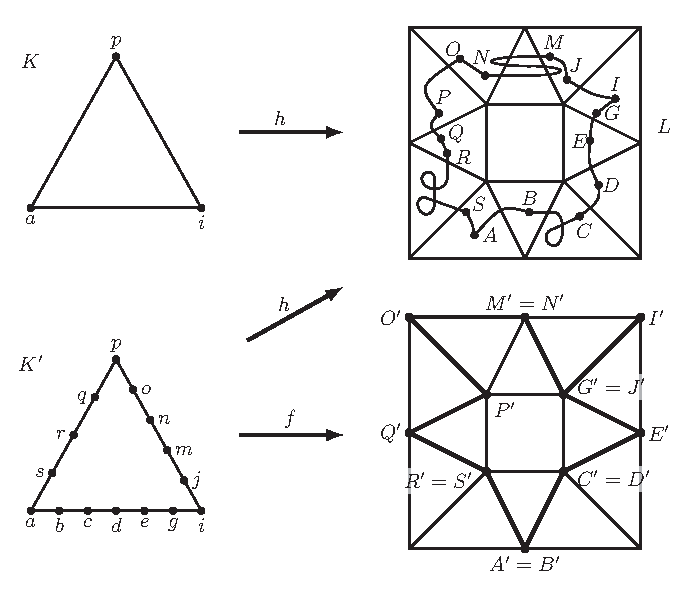
\includegraphics[width=119mm]{figures/2-2-1.pdf}\\图 2.2.1
\end{center}
若 $h$ 对 $K,L$ 满足星形条件，令 $h_*=f_*$，其中 $f$ 为任意单纯逼近，就得到良定义的同态 $h_*:H_p(K)\to H_p(L)$。容易看出它满足函子性质。

一般的连续映射 $h$ 不一定对 $K,L$ 满足星形条件，不能直接如此定义 $h_*$。怎么办？需要两个想法。

首先证明：给定 $h$，可将 $K$ “剖分”为底空间相同的新复形 $K'$，使 $h$ 对 $K',L$ 满足星形条件，正如例 2.2.6。此步骤是几何性的，将在第 2.3、2.4 节完成。

然后证明，恒等映射 $i:|K'|\to|K|$ 有一个诱导同调同构的单纯逼近 $g:K'\to K$。此步骤是代数性的，在第 2.5 节完成。最后定义
\[
h_*=f_*\circ g_*^{-1}:H_p(K)\to H_p(L).
\]
我们将在第 2.6 节看到，这个诱导同态也满足函子性质。

\subsection*{在相对同调中的应用}
上述单纯逼近结果直接推广到相对同调。

\entry{引理}{2.2.7}设 $h:|K|\to|L|$ 对 $K,L$ 满足星形条件，并将子复形的底空间 $|K_0|$ 映入 $|L_0|$。则：
\begin{enumerate}[label=(\alph*)]
\item 任意单纯逼近 $f:K\to L$ 也将 $|K_0|$ 映入 $|L_0|$，且其在 $K_0$ 上的限制是 $h|_{|K_0|}$ 的单纯逼近。
\item 任意两个单纯逼近 $f,g$ 作为偶的映射邻接。
\end{enumerate}
\sourcepage{97}
\noindent\textbf{证明：}给定 $\sigma\in K_0$，取 $x\in\Int\sigma$，令 $h(x)\in\Int\tau$。因为 $h$ 将 $|K_0|$ 映入 $|L_0|$，所以 $\tau\in L_0$。$f,g$ 都把 $\sigma$ 映到 $\tau$ 的面上，因此将 $K_0$ 映入 $L_0$，且作为偶的映射邻接。

再验证限制为单纯逼近。对 $K_0$ 的顶点 $v$，有 $\operatorname{St}(v,K_0)=\operatorname{St}(v,K)\cap|K_0|$，于是
\[
\begin{aligned}
h(\operatorname{St}(v,K_0))
&\subset h(\operatorname{St}(v,K))\cap h(|K_0|)\\
&\subset\operatorname{St}(f(v),L)\cap|L_0|\\
&=\operatorname{St}(f(v),L_0).
\end{aligned}
\]
得到所需结果。\hfill$\square$

下一个定义用于习题 2，并将在第 2.7 节再次出现。

\entry{定义}{2.2.8}映射 $f,h:X\to Y$ 之间的\textbf{同伦}（homotopy）是连续映射 $F:X\times I\to Y$，其中 $I=[0,1]$，使对每个 $x$ 有 $F(x,0)=f(x)$、$F(x,1)=h(x)$。下面 $(*)$ 定义的特定同伦称为\textbf{直线同伦}（straight-line homotopy）。

\subsection*{习题}
\begin{enumerate}
\item 考虑例 2.2.6 中的 $h:|K|\to|L|$，确定它有多少个不同的单纯逼近 $f:K'\to L$。设 $f,g$ 为两个逼近，选取生成 $H_1(K')$ 的闭链 $z$，找出 $L$ 的链 $d$，使 $\partial d=f_\#(z)-g_\#(z)$。\translatornote{原文选取闭链时误记为 $g$，与后面的公式不一致；这里统一为 $z$。}
\item \begin{enumerate}[label=(\alph*)]
\item 对映射 $f,h:X\to\R^N$，证明公式
\[
F(x,t)=(1-t)f(x)+th(x)\tag{$*$}
\]
定义两者之间的同伦，即直线同伦。
\item 设 $K,L$ 为 $\R^N$ 中的有限复形，$f:K\to L$ 为 $h:|K|\to|L|$ 的单纯逼近，证明 $(*)$ 定义两者之间的同伦。
\item[\textasteriskcentered\,(c)] 讨论 $K,L$ 不有限时的 (b)。
\end{enumerate}
\item 设 $f,h:\R\to\R^2$ 分别为 $f(x)=(x,x^3)$、$h(x)=(x,e^x)$，证明两者同伦。
\end{enumerate}

\section{重心剖分}
\sourcepage{98--99}
本节证明，有限复形可以“剖分”为任意小的单形。单纯同调的讨论中要用到此结果，第四章讨论奇异同调时也要用到。

\entry{定义}{2.3.1}设 $K$ 为 $E^J$ 中的几何复形。若复形 $K'$ 满足以下条件，则称为 $K$ 的\textbf{剖分}（subdivision）：
\begin{enumerate}[label=(\arabic*)]
\item $K'$ 的每个单形包含在 $K$ 的某个单形中。
\item $K$ 的每个单形是 $K'$ 中有限多个单形的并。
\end{enumerate}
这些条件蕴含两复形的单形之并相同，即 $|K'|=|K|$ 作为集合相等。条件 (2) 的有限性还保证两者作为拓扑空间相同，容易验证。

若 $K''$ 为 $K'$ 的剖分，$K'$ 为 $K$ 的剖分，则 $K''$ 为 $K$ 的剖分。

若 $K_0$ 是 $K$ 的子复形，则 $K'$ 中所有位于 $|K_0|$ 的单形自动构成 $K_0$ 的剖分，称为\textbf{由 $K'$ 诱导的 $K_0$ 的剖分}。

下面的结果后文有用。

\entry{引理}{2.3.2}设 $K'$ 为 $K$ 的剖分。对于 $K'$ 的每个顶点 $w$，存在 $K$ 的顶点 $v$，使
\[
\operatorname{St}(w,K')\subset\operatorname{St}(v,K).\tag{$*$}
\]
事实上，若 $w\in\Int\sigma$，其中 $\sigma\in K$，则此包含关系成立，当且仅当 $v$ 是 $\sigma$ 的顶点。

\noindent\textbf{证明：}若 $(*)$ 成立，因为 $w\in\operatorname{St}(w,K')$，所以 $w$ 位于以 $v$ 为顶点的某个开单形中。

反过来，设 $w\in\Int\sigma$，$v$ 为 $\sigma$ 的顶点。只需证明
\[
|K|\setminus\operatorname{St}(v,K)\subset|K|\setminus\operatorname{St}(w,K').
\]
左边是 $K$ 中所有不以 $v$ 为顶点的单形之并，因此也是 $K'$ 的某些单形 $\tau$ 的并。这样的 $\tau$ 不可能以 $w$ 为顶点，因为 $w\in\Int\sigma\subset\operatorname{St}(v,K)$。所以每个这样的单形都位于右边。\hfill$\square$

\entry{例}{2.3.3}设 $K$ 由 $1$ 维单形 $[0,1]$ 及其顶点组成。设 $L$ 由各 $[1/(n+1),1/n]$（$n=1,2,\ldots$）、它们的顶点以及顶点 $0$ 组成。则 $|L|=|K|$ 作为集合相同，但作为拓扑空间不同。$L$ 满足剖分的所有条件，唯独不满足条件 (2) 的有限性。

\entry{例}{2.3.4}设 $\Sigma$ 由 $2$ 维单形 $\sigma$ 及其各面组成。图 2.3.1 中 $\Bd\sigma$ 的剖分 $K$ 可扩张为 $\Sigma$ 的剖分 $\Sigma'$：取内部点 $w$，作锥 $w*K$ 即可。称其为\textbf{从 $w$ 对 $K$ 作星形剖分}（starring $K$ from $w$）。这种方法后面很有用。
\begin{center}
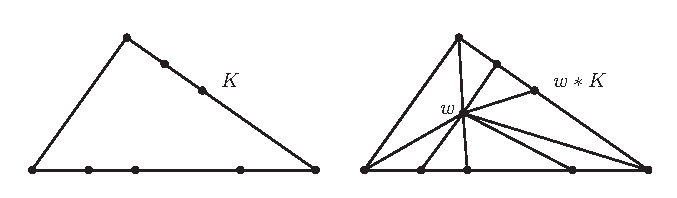
\includegraphics[width=117mm]{figures/2-3-1.pdf}\\图 2.3.1
\end{center}
下面描述一般复形的星形剖分方法，先需一个引理，证明留作习题。

\entry{引理}{2.3.5}复形 $K$ 的任意一族子复形的交仍为子复形。反过来，若 $\{K_\alpha\}$ 为 $E^J$ 中的一族复形，每一对底空间的交 $|K_\alpha|\cap|K_\beta|$ 都是同时为两者子复形的某个复形的多胞体，则并 $\bigcup_\alpha K_\alpha$ 为复形。

构造剖分采用逐步进行的方法，下面描述其中一步。

\entry{定义}{2.3.6}设 $L_p$ 是 $K$ 的 $p$ 维骨架的剖分。对于 $K$ 的 $(p+1)$ 维单形 $\sigma$，$\Bd\sigma$ 是 $p$ 维骨架的某个子复形的多胞体，因此也是 $L_p$ 的某个子复形的多胞体，以 $L_\sigma$ 表示后者。若 $w_\sigma\in\Int\sigma$，则锥 $w_\sigma*L_\sigma$ 的底空间为 $\sigma$。令 $L_{p+1}$ 为 $L_p$ 与所有这些锥的并。下面说明它是复形，称为\textbf{从各点 $w_\sigma$ 对 $L_p$ 作星形剖分而得到的 $K^{(p+1)}$ 的剖分}。

事实上，$|w_\sigma*L_\sigma|\cap|L_p|=\Bd\sigma$，它是同时为锥和 $L_p$ 的子复形 $L_\sigma$ 的多胞体。\translatornote{原文此处有 $W_p,W_\sigma,L_p$ 等下标、字母误印；这里按前述定义统一为 $w_\sigma,L_\sigma$。}若 $\tau$ 为另一个 $(p+1)$ 维单形，则两个锥的底空间相交于 $\sigma\cap\tau$，它是 $L_p$ 的某个子复形的多胞体，因此也同时对应 $L_\sigma,L_\tau$ 的子复形。由引理，$L_{p+1}$ 为复形。

\sourcepage{100--101}
$L_{p+1}$ 依赖各点 $w_\sigma$ 的选择。常取单形的典范内点，通常如下。

\entry{定义}{2.3.7}若 $\sigma=v_0\cdots v_p$，定义其\textbf{重心}（barycenter）为
\[
\widehat\sigma=\frac1{p+1}\sum_{i=0}^p v_i.
\]
这是关于各顶点的重心坐标都相等的内点。若 $\sigma$ 为边，$\widehat\sigma$ 为其中点；若为顶点，则 $\widehat\sigma=\sigma$。一般地，它也是 $\sigma$ 的质心，但本书不使用此事实。

\entry{定义}{2.3.8}设 $K$ 为复形，逐步定义其骨架的剖分。令 $L_0=K^{(0)}$。若 $L_p$ 已为 $p$ 维骨架的剖分，则从 $K$ 中各 $(p+1)$ 维单形的重心对 $L_p$ 作星形剖分，得到 $L_{p+1}$。由引理 2.3.5，各 $L_p$ 的并为 $K$ 的一个剖分，称为\textbf{第一次重心剖分}（first barycentric subdivision），记作 $\operatorname{sd}K$。

再对它作第一次重心剖分，得到 $\operatorname{sd}(\operatorname{sd}K)$，记为 $\operatorname{sd}^2K$，称为第二次重心剖分。类似定义任意正整数次剖分 $\operatorname{sd}^nK$。

有时需要明确描述第一次重心剖分的单形。用 $\sigma_1\succ\sigma_2$ 表示“$\sigma_2$ 为 $\sigma_1$ 的真面”。

\entry{引理}{2.3.9}$\operatorname{sd}K$ 恰由所有形如 $\widehat\sigma_1\widehat\sigma_2\cdots\widehat\sigma_n$ 的单形组成，其中 $\sigma_1\succ\sigma_2\succ\cdots\succ\sigma_n$。

\noindent\textbf{证明：}归纳。位于 $K^{(0)}$ 的剖分中的单形显然如此：它们是 $K$ 的顶点，且 $\widehat v=v$。假定结论对位于 $|K^{(p)}|$ 的单形成立。若 $\tau$ 位于 $|K^{(p+1)}|$ 而不位于 $|K^{(p)}|$，则它属于某个 $\widehat\sigma*L_\sigma$，其中 $\sigma$ 为 $(p+1)$ 维单形，$L_\sigma$ 为其真面复形的第一次重心剖分。由归纳假设，$L_\sigma$ 的单形形如 $\widehat\sigma_1\cdots\widehat\sigma_n$，其中各 $\sigma_i$ 都为 $\sigma$ 的真面，且依次为真面。因此 $\tau$ 形如 $\widehat\sigma\widehat\sigma_1\cdots\widehat\sigma_n$，正是所需形式。\hfill$\square$

\entry{例}{2.3.10}图 2.3.2 给出了复形 $K$ 及其前两次重心剖分。注意，第一次剖分的每个单形都有引理 2.3.9 的形式。还要注意，随着 $n$ 增大，$\operatorname{sd}^nK$ 的单形迅速变小。下面证明这是一般事实。
\begin{center}
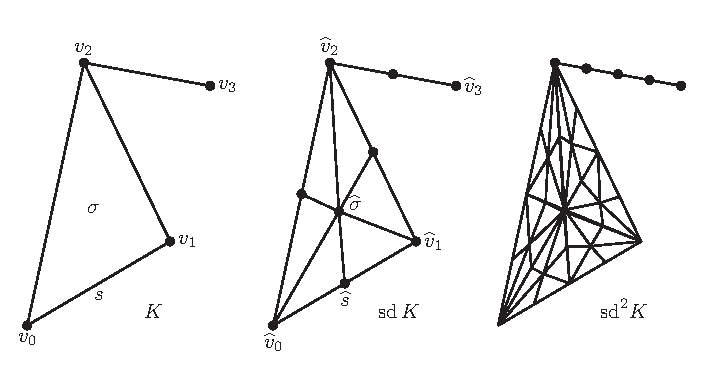
\includegraphics[width=122mm]{figures/2-3-2.pdf}\\图 2.3.2
\end{center}

\entry{定理}{2.3.11}给定有限复形 $K$、$|K|$ 的一个度量及 $\epsilon>0$，存在正整数 $N$，使 $\operatorname{sd}^NK$ 中每个单形的直径都小于 $\epsilon$。

\noindent\textbf{证明：}$K$ 有限，因此 $|K|$ 是其所在欧氏空间的子空间；又因为它紧致，选择哪个相容度量无关紧要。事实上，两个相容度量 $d_1,d_2$ 之间的恒等映射一致连续，给定 $\epsilon$，存在 $\delta>0$，使任何 $d_1$ 直径小于 $\delta$ 的集合，其 $d_2$ 直径小于 $\epsilon$。所以可用环境空间的度量
\[
|x-y|=\max_\alpha|x_\alpha-y_\alpha|.
\]
\textbf{第一步。}若 $\sigma=v_0\cdots v_p$，则其直径为顶点最大距离 $\ell=\max_{i,j}|v_i-v_j|$。显然 $\operatorname{diam}\sigma\geq\ell$，证明反向不等式。

先证对每个 $x\in\sigma$，$|x-v_i|\leq\ell$。以 $v_i$ 为中心、半径 $\ell$ 的闭邻域 $C(v_i;\ell)=\{x:|x-v_i|\leq\ell\}$ 是凸集，包含所有顶点，故包含 $\sigma$。

再固定 $x\in\sigma$。由刚才的结论，凸闭邻域 $C(x;\ell)$ 包含全部顶点，因此包含 $\sigma$。所以任意 $x,z\in\sigma$ 都满足 $|x-z|\leq\ell$，得到所需上界。

\sourcepage{102--103}
\textbf{第二步。}若 $\dim\sigma=p$，则每个 $z\in\sigma$ 满足
\[
|\widehat\sigma-z|\leq\frac p{p+1}\operatorname{diam}\sigma.
\]
计算
\[
\begin{aligned}
|v_0-\widehat\sigma|
&=\left|v_0-\sum_{i=0}^p\frac1{p+1}v_i\right|\\
&\leq\sum_{i=0}^p\frac1{p+1}|v_0-v_i|\\
&\leq\frac p{p+1}\max_i|v_0-v_i|
\leq\frac p{p+1}\operatorname{diam}\sigma.
\end{aligned}
\]
其他顶点也类似。因此以重心为中心、半径 $p\operatorname{diam}\sigma/(p+1)$ 的凸闭邻域包含全部顶点，故包含 $\sigma$。

\textbf{第三步。}若 $\sigma$ 为 $p$ 维单形，$\tau$ 为其第一次重心剖分的单形，则
\[
\operatorname{diam}\tau\leq\frac p{p+1}\operatorname{diam}\sigma.
\]
对维数归纳。$p=0$ 平凡。假定低于 $p$ 的维数成立。由引理 2.3.9 与第一步，只需对 $\sigma$ 的面 $s\succ s'$ 证明
\[
|\widehat s-\widehat{s'}|\leq\frac p{p+1}\operatorname{diam}\sigma.
\]
若 $s=\sigma$，由第二步得到。若 $s$ 为 $q$ 维真面，则
\[
|\widehat s-\widehat{s'}|\leq\frac q{q+1}\operatorname{diam}s
\leq\frac p{p+1}\operatorname{diam}\sigma.
\]
第一个不等式由归纳假设，第二个因为 $x/(x+1)$ 对 $x>0$ 递增。

\textbf{第四步。}设 $\dim K=n$，其单形最大直径为 $d$。第 $N$ 次重心剖分中单形的最大直径不超过 $(n/(n+1))^Nd$。\translatornote{原文将此表达式直接写为最大直径；前面证明给出的是上界，这已足够。}$N$ 足够大时，小于 $\epsilon$。\hfill$\square$

以下定义用于习题 2、3。

\entry{定义}{2.3.12}
\begin{enumerate}[label=(\arabic*)]
\item 对集合族 $\mathcal A,\mathcal B$，若每个 $B\in\mathcal B$ 都包含于某个 $A\in\mathcal A$，则称 $\mathcal B$ \textbf{加细} $\mathcal A$（refines）。
\item 若存在整数 $m$，使空间 $X$ 的每个开覆盖 $\mathcal A$ 都有一个开覆盖加细 $\mathcal B$，且 $X$ 中没有点属于 $\mathcal B$ 的多于 $m+1$ 个成员，则称 $X$ 具有\textbf{有限覆盖维数}。
\item 满足 (2) 的最小整数 $m$ 称为 $X$ 的\textbf{覆盖维数}（covering dimension）。
\end{enumerate}
习题 3 涉及 Cantor 三分集。为完整起见给出定义，得到的就是通常“不断去掉中间三分之一”的集合。

\entry{定义}{2.3.13}对每个正整数 $m$，令
\[
C_m=\bigcup_{k=0}^{(3^m-1)/2}\left[\frac{2k}{3^m},\frac{2k+1}{3^m}\right].
\]
\textbf{Cantor 三分集}定义为 $C=\bigcap_{m=1}^\infty C_m$。

\subsection*{习题}
\begin{enumerate}
\item 设 $K$ 为复形，$x_0\in|K|$。
\begin{enumerate}[label=(\alph*)]
\item 证明存在顶点集包含 $x_0$ 的剖分。
\item[\textasteriskcentered\,(b)] 证明存在顶点集恰由 $x_0$ 和 $K$ 的原有顶点组成的剖分。
\end{enumerate}
\item \begin{enumerate}[label=(\alph*)]
\item 证明离散集的覆盖维数为 $0$。
\item 证明 $[0,1]$ 的覆盖维数为 $1$。
\item 若 $X$ 的覆盖维数为 $m$，证明其任意闭子空间 $A$ 的覆盖维数至多为 $m$。
\item 若 $K$ 为 $m$ 维有限复形，证明 $|K|$ 的覆盖维数存在且至多为 $m$。［后面将看到它恰好为 $m$。］
\end{enumerate}
\item 计算 Cantor 三分集的覆盖维数。
\end{enumerate}

\section{单纯逼近定理}
\sourcepage{104--105}
现在证明：若 $h:|K|\to|L|$ 连续，则存在 $K$ 的剖分 $K'$，使 $h$ 有单纯逼近 $f:K'\to L$。$K$ 有限时，由上一节容易得到，重心剖分即可满足要求。一般情形需要稍精细的“广义重心剖分”，见定义 2.4.5。

先需下面的引理。

\entry{引理}{2.4.1（Lebesgue 覆盖引理）}对紧致度量空间的每个开覆盖 $\mathcal A$，存在正实数 $\lambda$，使每个直径小于 $\lambda$ 的子集都包含在 $\mathcal A$ 的某个成员中。称 $\lambda$ 为此覆盖的一个 \textbf{Lebesgue 数}。

\noindent\textbf{证明：}若不存在，则可选择一列集合 $C_n$，使其直径小于 $1/n$，却不包含在任何覆盖成员中。选 $x_n\in C_n$，由紧致性，某个子列 $x_{n_i}$ 收敛于一点 $x$。取覆盖成员 $A$ 包含 $x$，因为 $A$ 开，当 $i$ 足够大时 $C_{n_i}\subset A$，与构造矛盾。\hfill$\square$

\entry{定理}{2.4.2（有限单纯逼近定理）}设 $K,L$ 为复形，$K$ 有限。给定连续映射 $h:|K|\to|L|$，存在 $N$，使其有单纯逼近 $f:\operatorname{sd}^NK\to L$。

\noindent\textbf{证明：}以所有 $h^{-1}(\operatorname{St}w)$ 覆盖 $|K|$，其中 $w$ 遍历 $L$ 的顶点。令 $\lambda$ 为此开覆盖的 Lebesgue 数。选择 $N$ 使 $\operatorname{sd}^NK$ 的每个单形直径小于 $\lambda/2$，则每个顶点的星形邻域直径小于 $\lambda$，从而位于某个 $h^{-1}(\operatorname{St}w)$ 内。于是 $h$ 对 $\operatorname{sd}^NK,L$ 满足星形条件，所需逼近存在。\hfill$\square$

作为推广重心剖分的准备，先说明如何在保持给定子复形 $K_0$ 不变的同时剖分 $K$。

\entry{定义}{2.4.3}令 $J_0=K^{(0)}$。一般地，设 $J_p$ 为 $K$ 的 $p$ 维骨架的剖分，且包含 $K_0$ 中维数至多为 $p$ 的每个单形。定义 $J_{p+1}$ 为以下各族的并：$J_p$；属于 $K_0$ 的所有 $(p+1)$ 维单形；以及对所有不属于 $K_0$ 的 $(p+1)$ 维单形 $\sigma$ 作出的锥 $\widehat\sigma*J_\sigma$，其中 $|J_\sigma|=\Bd\sigma$。各 $J_p$ 的并为 $K$ 的剖分，记为 $\operatorname{sd}(K/K_0)$，称为\textbf{保持 $K_0$ 不变的第一次重心剖分}。

此过程可以重复，$\operatorname{sd}(\operatorname{sd}(K/K_0)/K_0)$ 称为保持 $K_0$ 不变的第二次重心剖分，记为 $\operatorname{sd}^2(K/K_0)$，其余类似。

\entry{例}{2.4.4}图 2.4.1 展示了 $K$ 的第一次重心剖分及保持 $K_0$ 不变的第一次重心剖分。
\begin{center}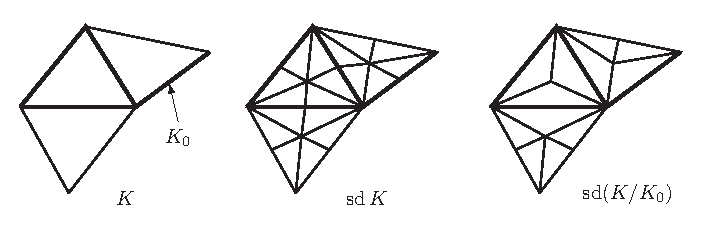
\includegraphics[width=123mm]{figures/2-4-1.pdf}\\图 2.4.1\end{center}
一般单纯逼近定理不能仅靠反复重心剖分证明，因为定理 2.4.2 的 Lebesgue 数论证要求 $|K|$ 紧致。对一般复形，每个单形所需剖分精细程度可能不同，必须允许这种差异。

\entry{定义}{2.4.5}设函数 $N$ 为 $K$ 的每个正维单形 $\sigma$ 指定非负整数 $N(\sigma)$。令 $L_0=K^{(0)}$。设 $L_p$ 为 $p$ 维骨架的剖分，对每个 $(p+1)$ 维单形 $\sigma$，取 $L_p$ 中底空间为 $\Bd\sigma$ 的子复形 $L_\sigma$，先形成锥 $\widehat\sigma*L_\sigma$，再保持 $L_\sigma$ 不变，对此锥作 $N(\sigma)$ 次重心剖分。令 $L_{p+1}$ 为 $L_p$ 与所有
\[
\operatorname{sd}^{N(\sigma)}(\widehat\sigma*L_\sigma/L_\sigma)
\]
的并。于是 $L_{p+1}$ 为 $(p+1)$ 维骨架的剖分，而各 $L_p$ 的并为 $K$ 的剖分，称为\textbf{相应于函数 $N(\sigma)$ 的广义重心剖分}（generalized barycentric subdivision）。

\sourcepage{106}
本节余下部分说明，这种剖分足以证明一般单纯逼近定理。比较下列复形时，可参照图 2.4.1。

\entry{引理}{2.4.6}设 $K_0$ 为 $K$ 的子复形。
\begin{enumerate}[label=(\alph*)]
\item $\operatorname{sd}(K/K_0)$ 的每个单形 $\tau$ 都形如
\[
\tau=\widehat\sigma_1\widehat\sigma_2\cdots\widehat\sigma_q v_0v_1\cdots v_p,
\]
其中 $s=v_0\cdots v_p$ 为 $K_0$ 的单形，各 $\sigma_j$ 是 $K$ 中不属于 $K_0$ 的单形，且 $\sigma_1\succ\cdots\succ\sigma_q\succ s$。
\item 表达式中的 $v_0\cdots v_p$ 或 $\widehat\sigma_1\cdots\widehat\sigma_q$ 可以缺失。$\tau$ 与 $|K_0|$ 不交，当且仅当前一部分缺失；此时 $\tau$ 是 $\operatorname{sd}K$ 的单形。
\end{enumerate}
\noindent\textbf{证明：}(a) 对 $J_0$ 中的单形成立。一般地，若 $\tau\in J_{p+1}\setminus J_p$，则它或者属于 $K_0$，已有所需形式；或者属于某个锥 $\widehat\sigma*J_\sigma$。由归纳假设，$J_\sigma$ 的单形已有所需形式，且其最大面为 $\sigma$ 的真面，添加顶点 $\widehat\sigma$ 后仍是所需形式。

(b) 若后一部分顶点 $v_i$ 存在，则 $\tau$ 至少在 $v_0\cdots v_p$ 上与 $|K_0|$ 相交。反过来，若交非空，则其中包含 $\tau$ 的一个面，因而包含一个顶点。各 $\widehat\sigma_j$ 都不属于 $|K_0|$，故某个 $v_i$ 必须存在。\hfill$\square$

证明一般单纯逼近定理，需要使开星形邻域族加细覆盖
\[
\mathcal A=\{h^{-1}(\operatorname{St}(w,L)):w\text{ 为 }L\text{ 的顶点}\}.
\]
实际上将证明更强的结论：存在剖分 $K'$，使闭星形邻域族 $\{\overline{\operatorname{St}(v,K')}\}$ 加细 $\mathcal A$。下面的引理是归纳步骤的关键。

\sourcepage{107--108}
\entry{引理}{2.4.7}设 $K=p*B$ 为有限复形 $B$ 上的锥，$\mathcal A$ 为 $|K|$ 的开覆盖。假定对 $B$ 的每个顶点 $v$，指定了 $A_v\in\mathcal A$，满足 $\overline{\operatorname{St}(v,B)}\subset A_v$。则存在 $N$，使 $\operatorname{sd}^N(K/B)$ 的闭星形邻域族加细 $\mathcal A$，并且对 $B$ 的每个顶点 $v$，有
\[
\overline{\operatorname{St}(v,\operatorname{sd}^N(K/B))}\subset A_v.
\]
\noindent\textbf{证明：}设 $|B|\subset\R^m\times\{0\}$，$n=\dim K$，取锥顶 $p=(0,\ldots,0,1)\in\R^m\times\R$。

\textbf{第一步。}随着 $N$ 增大，最大单形直径一般不趋于零，因为 $B$ 中的正维面始终不剖分。不过，与平面 $\R^m\times\{0\}$ 相交的单形会越来越贴近该平面。更一般地，设 $K'$ 是保持 $B$ 不变的剖分，且所有与该平面相交的单形都位于条带 $\R^m\times[0,\epsilon]$ 内。则 $\operatorname{sd}(K'/B)$ 中与此平面相交的单形 $\tau$，都位于 $\R^m\times[0,n\epsilon/(n+1)]$ 内。

由引理 2.4.6，$\tau$ 形如 $\widehat\sigma_1\cdots\widehat\sigma_qv_0\cdots v_p$。\translatornote{原文此处误引为引理 2.5.5。}若它与平面相交而不完全位于平面内，则两部分都不缺失，各 $v_i$ 位于平面内。每个 $\sigma_j$ 都以 $v_0\cdots v_p$ 为面，故与平面相交，位于上述条带。设其顶点为 $w_0,\ldots,w_k$，$\pi$ 为最后坐标投影。各 $\pi(w_i)\leq\epsilon$，至少一个为零，因此
\[
\pi(\widehat\sigma_j)=\sum_{i=0}^k\frac1{k+1}\pi(w_i)
\leq\frac k{k+1}\epsilon\leq\frac n{n+1}\epsilon.
\]
$\tau$ 的全部顶点都位于所需凸条带内，故整个单形也位于其中。

\textbf{第二步。}记 $K_N=\operatorname{sd}^N(K/B)$。证明存在 $N_0$，当 $N\geq N_0$ 时，对 $B$ 的每个顶点 $v$，有
\[
\overline{\operatorname{St}(v,K_N)}\subset A_v.\tag{$*$}
\]
先断言，可选择 $\delta>0$，使对每个 $v$，
\[
\overline{\operatorname{St}(v,K)}\cap(\R^m\times[0,\delta])\subset A_v,
\]
见图 2.4.2。
\begin{center}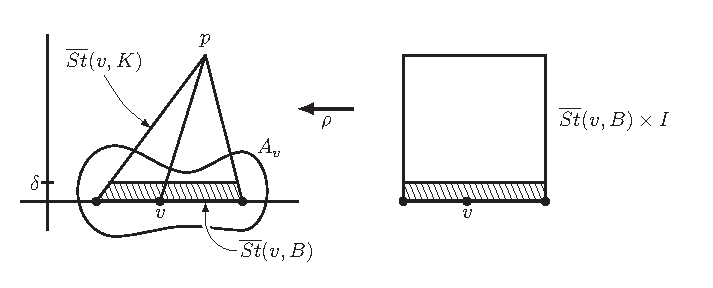
\includegraphics[width=123mm]{figures/2-4-2.pdf}\\图 2.4.2\end{center}
考察连续映射 $\rho:|B|\times I\to|K|$，$\rho(x,t)=(1-t)x+tp$。因为 $K$ 为锥，它把 $\overline{\operatorname{St}(v,B)}\times I$ 映到 $\overline{\operatorname{St}(v,K)}$ 上，并保持最后坐标：
\[
\pi\rho(x,t)=(1-t)\pi(x)+t\pi(p)=(1-t)0+t1=\pi(x,t).
\]
闭星形邻域 $\overline{\operatorname{St}(v,B)}$ 紧致，由一般拓扑的管状引理［例如 [Mun00] 第 26 节］，可选取 $\delta>0$，使
\[
\overline{\operatorname{St}(v,B)}\times[0,\delta]\subset\rho^{-1}(A_v).
\]
更直接地，可用有限多个包含于 $\rho^{-1}(A_v)$ 的集合 $U_i\times[0,\delta_i]$ 覆盖底部，再取 $\delta=\min_i\delta_i$。因为 $B$ 的顶点有限，也可令 $\delta$ 对所有顶点同时适用。于是
\[
\rho(\overline{\operatorname{St}(v,B)}\times[0,\delta])
=\overline{\operatorname{St}(v,K)}\cap(\R^m\times[0,\delta])\subset A_v.
\]
由第一步选择 $N_0$，使 $N\geq N_0$ 时，与底平面相交的各单形都位于此条带。故闭星形邻域 $\overline{\operatorname{St}(v,K_N)}$ 同时位于条带与 $\overline{\operatorname{St}(v,K)}$，所以位于 $A_v$，证明 $(*)$。

\sourcepage{109}
\textbf{第三步。}固定 $N_0$，考察 $K_{N_0+1}$。令 $Q$ 为其中所有与 $B$ 不交的单形的并，见图 2.4.3。用 $P$ 表示图中其余靠近底部的闭区域，即所有与 $B$ 相交的单形之并。\translatornote{原文使用图中的 $P$，但没有在正文中明确给出定义；这里按图及后续论证补明。}
\begin{center}
\begin{minipage}{.47\textwidth}\centering
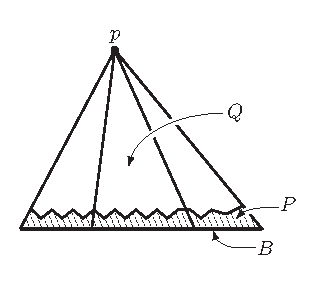
\includegraphics[width=59mm]{figures/2-4-3.pdf}\\图 2.4.3
\end{minipage}\hfill
\begin{minipage}{.47\textwidth}\centering
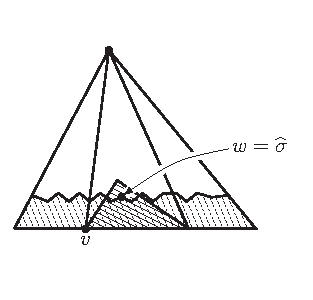
\includegraphics[width=57mm]{figures/2-4-4.pdf}\\图 2.4.4
\end{minipage}
\end{center}
证明：若 $N\geq N_0+1$，$w$ 为 $K_N$ 中位于 $P\setminus|B|$ 的顶点，则存在 $A\in\mathcal A$，使
\[
\overline{\operatorname{St}(w,K_N)}\subset A.\tag{$**$}
\]
先设 $N=N_0+1$。$P$ 按定义是子复形的多胞体。由引理 2.4.6，位于 $P$ 但不在 $B$ 的顶点 $w$ 为某个 $K_{N_0}$ 单形 $\sigma$ 的重心，该 $\sigma$ 与 $B$ 相交而不包含于 $B$，见图 2.4.4。选取其一个位于 $B$ 的顶点 $v$，由引理 2.3.2，
\[
\operatorname{St}(w,K_{N_0+1})\subset\operatorname{St}(v,K_{N_0}).
\]
取闭包，再用第二步，得 $\overline{\operatorname{St}(w,K_{N_0+1})}\subset\overline{\operatorname{St}(v,K_{N_0})}\subset A_v$。

若 $N>N_0+1$，则 $P$ 中的顶点 $w'$ 位于 $K_{N_0+1}$ 的某个顶点 $w$ 的星形邻域内，可取 $w$ 位于 $P$。由引理 2.3.2，$\operatorname{St}(w',K_N)\subset\operatorname{St}(w,K_{N_0+1})$，取闭包后由前段，或 $w\in B$ 时由第二步，得到 $(**)$。

\textbf{第四步。}令 $\lambda$ 为覆盖的 Lebesgue 数。$Q$ 是 $K_{N_0+1}$ 的某个子复形 $J$ 的多胞体。由引理 2.4.6，形成 $K_{N_0+2}$ 时，$J$ 的每个单形都作普通重心剖分，因此 $\operatorname{sd}J$ 为其子复形。重复可知，$\operatorname{sd}^MJ$ 为 $K_{N_0+1+M}$ 的子复形。

选取足够大的 $M$，使 $\operatorname{sd}^MJ$ 的每个单形直径小于 $\lambda/2$。若 $N\geq N_0+1+M$ 且 $w\notin P$，则存在 $A\in\mathcal A$，使
\[
\overline{\operatorname{St}(w,K_N)}\subset A.\tag{$***$}
\]
因为每个以 $w$ 为顶点的单形均位于 $Q$，并包含于上述细剖分的单形中，所以闭星形邻域直径小于 $\lambda$，位于某个覆盖成员中。综合 $(*)$、$(**)$、$(***)$ 即得引理。\hfill$\square$

\sourcepage{110--111}
\entry{定理}{2.4.8}设 $K$ 为复形，$\mathcal A$ 为 $|K|$ 的开覆盖。存在广义重心剖分 $K'$，使其闭星形邻域族加细 $\mathcal A$。

\noindent\textbf{证明：}逐步构造。先令 $L_0=K^{(0)}$，为每个顶点 $v$ 选择包含它的覆盖成员 $A_v$。

一般地，设已给定 $K^{(p)}$ 的剖分 $L_p$，以及为每个顶点 $v$ 指定 $A_v\in\mathcal A$ 的函数 $f_p$，满足 $\overline{\operatorname{St}(v,L_p)}\subset A_v$。下面扩张到 $L_{p+1}$ 及 $f_{p+1}$。

对于每个 $(p+1)$ 维单形 $\sigma$，其边界为 $L_p$ 的某个子复形 $L_\sigma$ 的多胞体。对锥 $\widehat\sigma*L_\sigma$，由引理存在 $N(\sigma)$，使
\[
C(\sigma)=\operatorname{sd}^{N(\sigma)}(\widehat\sigma*L_\sigma/L_\sigma)
\]
满足：若顶点 $v\in L_\sigma$，则 $\overline{\operatorname{St}(v,C(\sigma))}\subset A_v$；对于其他顶点 $w$，存在某个 $A\in\mathcal A$ 包含其闭星形邻域。

令 $L_{p+1}$ 为 $L_p$ 与所有 $C(\sigma)$ 的并。若 $v$ 是旧顶点，则其新闭星形邻域为 $\overline{\operatorname{St}(v,L_p)}$ 与所有包含 $v$ 的相应 $\overline{\operatorname{St}(v,C(\sigma))}$ 的并，全部位于 $A_v$。若 $w$ 为新顶点，则它位于某个 $\sigma$ 的内部，且
\[
\overline{\operatorname{St}(w,L_{p+1})}
=\overline{\operatorname{St}(w,C(\sigma))}.
\]
选取包含它的覆盖成员 $A_w$，定义 $f_{p+1}(w)=A_w$。归纳步骤完成。

取 $K'=\bigcup_p L_p$，函数 $f$ 为各 $f_p$ 的并。若 $v$ 是 $L_p$ 的顶点，则对所有 $k\geq0$，有 $\overline{\operatorname{St}(v,L_{p+k})}\subset f_{p+k}(v)=f(v)=A_v$。因此 $\overline{\operatorname{St}(v,K')}\subset A_v$，定理得证。\hfill$\square$

\entry{定理}{2.4.9（一般单纯逼近定理）}设 $K,L$ 为复形，$h:|K|\to|L|$ 连续。存在 $K$ 的剖分 $K'$，使 $h$ 有单纯逼近 $f:K'\to L$。

\noindent\textbf{证明：}用开集 $h^{-1}(\operatorname{St}(w,L))$ 覆盖 $|K|$，选择闭星形邻域族加细此覆盖的剖分 $K'$。于是 $h$ 对 $K',L$ 满足星形条件。\hfill$\square$

\subsection*{习题}
\begin{enumerate}
\item \begin{enumerate}[label=(\alph*)]
\item 用定理 2.4.2 证明：若 $K,L$ 有限，$\dim K=m$，则每个连续映射 $h:|K|\to|L|$ 同伦于将 $K$ 映入 $L^{(m)}$ 的映射。［提示：第 2.2 节习题 2。非有限情形后面讨论。］
\item 证明：若 $h:S^m\to S^n$ 且 $m<n$，则 $h$ 同伦于常值映射。［提示：任意 $f:X\to S^n\setminus\{p\}$ 同伦于常值映射。］
\end{enumerate}
\item 若 $h:|K|\to|L|$ 连续，给定 $\epsilon>0$，证明存在两者的剖分 $K',L'$ 以及单纯映射 $f:K'\to L'$，使对所有 $x$ 有 $|f(x)-h(x)|<\epsilon$。
\item 证明：若 $\dim K=m$，则 $|K|$ 的覆盖维数至多为 $m$，见第 2.3 节习题。
\item 举例说明习题 3 的结论是最佳的。
\end{enumerate}

\section{剖分的代数}
\sourcepage{111--112}
现在研究剖分的代数后果，确定它对同调群的作用。将证明：对任意复形 $K$ 及其剖分 $K'$，存在唯一确定的链映射 $\lambda:C_p(K)\to C_p(K')$，称为\textbf{剖分算子}（subdivision operator），它诱导同调同构。此外，若 $g:K'\to K$ 为底空间恒等映射的任意单纯逼近，则 $\lambda,g_\#$ 互为链同伦逆，所以 $g_*$ 也是同构。\translatornote{原文此句写 $g_\#$ 为同构；这里应指诱导的同调映射 $g_*$。}

\entry{引理}{2.5.1}设 $K'$ 为 $K$ 的剖分，则恒等映射 $i:|K|\to|K|$ 有单纯逼近 $g:K'\to K$。若 $\tau\in K'$、$\sigma\in K$ 且 $\tau\subset\sigma$，则 $g(\tau)\subset\sigma$。

\noindent\textbf{证明：}由引理 2.3.2，单纯逼近存在。给定 $\tau\subset\sigma$，若 $w$ 为 $\tau$ 的顶点，它位于 $\sigma$ 或其某个面的内部，由引理 2.2.2，$g(w)$ 为 $\sigma$ 的顶点。\hfill$\square$

\entry{定义}{2.5.2}对 $\sigma\in K$，令 $K(\sigma)$ 为由 $\sigma$ 及其各面组成的子复形，令 $K'(\sigma)$ 为 $K'$ 中多胞体等于 $\sigma$ 的子复形。

\entry{定理}{2.5.3（代数剖分定理）}设 $K'$ 为 $K$ 的剖分。存在唯一的保持增广链映射 $\lambda:\mathcal C(K)\to\mathcal C(K')$，使每个 $\lambda(\sigma)$ 都由 $K'(\sigma)$ 承载。若 $g:K'\to K$ 为恒等映射的单纯逼近，则 $\lambda,g_\#$ 互为链同伦逆，故 $\lambda_*,g_*$ 都为同构。称 $\lambda$ 为\textbf{剖分算子}。

\noindent\textbf{证明：第一步。}先在下述额外条件下证明定理：对每个 $\sigma\in K$，诱导剖分 $K'(\sigma)$ 无环。使用几何形式的无环载体定理 1.14.10。

先定义 $K\to K$ 的载体 $\Psi(\sigma)=K(\sigma)$，以及 $K\to K'$ 的载体 $\Lambda(\sigma)=K'(\sigma)$。前者无环，因为由一个单形及其面组成；后者根据额外假设无环。面包含条件也显然成立。

为定义从 $K'$ 出发的两个载体，对于 $\tau\in K'$，令 $\sigma_\tau$ 为包含 $\tau$ 的最低维 $K$ 单形。若 $t$ 为 $\tau$ 的面，则 $\sigma_t\subset\sigma_\tau$：两者的交包含 $t$，由 $\sigma_t$ 的最小维数，它必须等于此交。令
\[
\Theta(\tau)=K(\sigma_\tau),\qquad\Phi(\tau)=K'(\sigma_\tau).
\]
两者均无环，面包含条件由上述包含关系得到。图 2.5.1 展示了 $K'=\operatorname{sd}K$ 的情形。
\begin{center}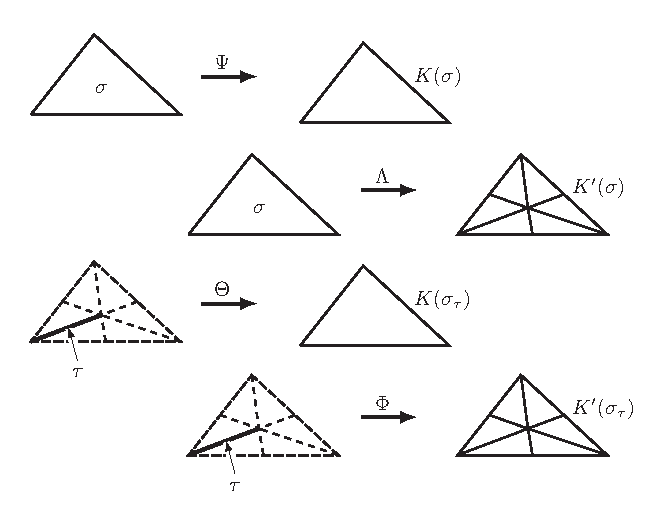
\includegraphics[width=116mm]{figures/2-5-1.pdf}\\图 2.5.1\end{center}
由无环载体定理，存在分别由 $\Lambda,\Theta$ 承载的保持增广链映射
\[
\lambda:\mathcal C(K)\to\mathcal C(K'),\qquad
\theta:\mathcal C(K')\to\mathcal C(K).
\]

\sourcepage{113--114}
$\mathcal C(K)$ 的恒等映射显然由 $\Psi$ 承载，复合 $\theta\lambda$ 也如此，因此两者链同伦。具体地，$\lambda(\sigma)$ 是 $K'(\sigma)$ 的链，其中每个单形 $\tau$ 都位于 $\sigma$ 内，故 $\sigma_\tau$ 是 $\sigma$ 或其面。因此 $\theta(\tau)$ 由 $K(\sigma_\tau)\subset K(\sigma)$ 承载，$\theta\lambda(\sigma)$ 也由 $K(\sigma)$ 承载。

同样，$\mathcal C(K')$ 的恒等映射由 $\Phi$ 承载，因为 $\tau\subset\sigma_\tau$，故 $\tau\in K'(\sigma_\tau)$。复合 $\lambda\theta$ 也由 $\Phi$ 承载：$\theta(\tau)$ 是 $\sigma_\tau$ 的各定向面的和，每个面 $s$ 的像 $\lambda(s)$ 由 $K'(s)\subset K'(\sigma_\tau)$ 承载。因此 $\lambda\theta$ 链同伦于恒等映射。

上述论证与所选择的具体 $\theta,\lambda$ 无关。$\theta$ 的一个选择是 $g_\#$，由前一引理它由 $\Theta$ 承载。所以 $g_\#,\lambda$ 互为链同伦逆。

再证唯一性。若 $\lambda'$ 为另一个由 $\Lambda$ 承载的保持增广链映射，则存在同样由 $\Lambda$ 承载的链同伦 $D$。对 $p$ 维单形 $\sigma$，$K'(\sigma)$ 维数为 $p$，而 $D\sigma$ 是由其承载的 $(p+1)$ 维链，只能为零。因此 $D=0$，由链同伦等式得 $\lambda=\lambda'$。

\textbf{第二步。}证明 $K'=\operatorname{sd}K$ 时成立。对 $\sigma\in K$，$K'(\sigma)$ 为锥 $\widehat\sigma*J$，其中 $J$ 为边界的第一次重心剖分，所以由定理 1.9.6 无环。［零维情形为单点复形。］这正是证明必须使用重心剖分之处。

\textbf{第三步。}证明 $K'=\operatorname{sd}^NK$ 时成立。由第一步，只需证明每个 $\operatorname{sd}^NK(\sigma)$ 无环。由第二步，对任意复形 $L$，
\[
\widetilde H_i(L)\cong\widetilde H_i(\operatorname{sd}L)
\cong\widetilde H_i(\operatorname{sd}^2L)\cong\cdots.
\]
所以 $L$ 无环时，其各次重心剖分也无环。

\textbf{第四步。}证明一般情形。仍只需证明任意诱导剖分 $K'(\sigma)$ 无环。令 $L=K(\sigma)$、$L'=K'(\sigma)$，已知 $L$ 无环，要证明 $L'$ 无环。取恒等映射的单纯逼近 $g:L'\to L$。由有限单纯逼近定理，选择 $N$ 使恒等映射有单纯逼近 $f:\operatorname{sd}^NL\to L'$；类似地，再选择 $M$，使其有逼近 $k:\operatorname{sd}^M(L')\to\operatorname{sd}^NL$。得到
\[
\operatorname{sd}^M(L')\xrightarrow{k}\operatorname{sd}^NL
\xrightarrow{f}L'\xrightarrow{g}L.
\]
\sourcepage{115--116}
复合 $gf$ 为恒等映射的单纯逼近，由第三步，$g_*f_*$ 为同构；同理 $f_*k_*$ 为同构。前者说明 $f_*$ 单射，后者说明它满射，因此 $f_*$ 为同构。于是 $g_*$ 也为同构，故 $L'$ 无环。\hfill$\square$

\entry{定义}{2.5.4}当 $K'=\operatorname{sd}K$ 时，将剖分算子记为 $\operatorname{sd}:C_p(K)\to C_p(\operatorname{sd}K)$，称为\textbf{重心剖分算子}。这里滥用记号，同时以 sd 表示代数与几何剖分算子。

它有归纳公式：
\[
\operatorname{sd}(v)=v,\qquad
\operatorname{sd}(\sigma)=[\widehat\sigma,\operatorname{sd}(\partial\sigma)].
\]
括号记号与第 1.9 节相同，此公式的验证留作习题。

\subsection*{在相对同调中的应用}
上述结果直接推广到相对同调。

\entry{定理}{2.5.5}设 $K_0$ 为 $K$ 的子复形，$K'$ 为 $K$ 的剖分，$K'_0$ 为其诱导的 $K_0$ 剖分。算子 $\lambda$ 诱导链映射
\[
\lambda:C_p(K,K_0)\to C_p(K',K'_0).
\]
若 $g:(K',K'_0)\to(K,K_0)$ 为恒等映射的任意单纯逼近，则 $\lambda,g_\#$ 互为链同伦逆。

\noindent\textbf{证明：}验证第一步中的各载体保持相应子复形。若 $\sigma\in K_0$，则 $\Psi(\sigma)=K(\sigma)$、$\Lambda(\sigma)=K'(\sigma)$ 分别为 $K_0,K'_0$ 的子复形。若 $\tau\in K'_0$，则它位于 $K_0$ 的某个单形中，因此包含它的最低维单形 $\sigma_\tau$ 属于 $K_0$。所以 $\Theta(\tau),\Phi(\tau)$ 也分别为 $K_0,K'_0$ 的子复形。

故 $\lambda,\theta$ 诱导相对链映射，而复合与恒等映射之间的链同伦也诱导相对链同伦。可选 $\theta=g_\#$，所以相对层次上 $g_\#,\lambda$ 互为链同伦逆。\hfill$\square$

\subsection*{习题}
\begin{enumerate}
\item 设 $K'$ 为 $K$ 的剖分，$\lambda$ 为剖分算子，$g:K'\to K$ 为恒等映射的单纯逼近。证明 $g_\#\lambda$ 等于 $C_p(K)$ 的恒等映射。
\item 图 2.5.2 中 $K,K'$ 的共同底空间为正方形区域。
\begin{enumerate}[label=(\alph*)]
\item 求剖分算子 $\lambda:C_p(K)\to C_p(K')$ 的公式。
\item 找出两个不同的恒等映射单纯逼近 $g,g':K'\to K$，说明代数剖分定理中的链等价 $\theta$ 不唯一。
\item 验证 $\lambda g_\#$ 不等于 $K'$ 链群上的恒等映射。
\end{enumerate}
\begin{center}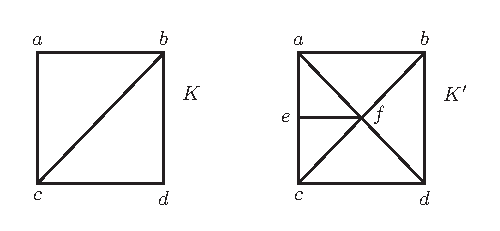
\includegraphics[width=90mm]{figures/2-5-2.pdf}\\图 2.5.2\end{center}
\item \begin{enumerate}[label=(\alph*)]
\item 证明重心剖分算子的归纳公式定义了由 $\Lambda$ 承载的保持增广链映射。
\item 对 $1$ 维、$2$ 维单形分别计算 $\operatorname{sd}\sigma$。
\end{enumerate}
\item 设 $K$ 为五边形区域［一维图形］，$K'$ 为同一五边形区域由两条对角线划分而成的复形。对它们回答习题 2(a)、(b)、(c)。\translatornote{原文写作“a pentagonal region square [the 1-dimensional figure]”，文字与维数说明互相矛盾。这里保留其意向而不擅自指定新的复形；若意在类比习题 2，应取同一填充五边形的两种剖分。}
\end{enumerate}

\section{同调群的拓扑不变性}
\sourcepage{117--118}
本节实现本章的主要目标：证明单纯同调群的拓扑不变性。

\entry{定义}{2.6.1}设 $K,L$ 为单纯复形，$h:|K|\to|L|$ 连续。选择 $K$ 的剖分 $K'$，使 $h$ 有单纯逼近 $f:K'\to L$。令 $\lambda:\mathcal C(K)\to\mathcal C(K')$ 为剖分算子。定义\textbf{由 $h$ 诱导的同态}
\[
h_*:H_p(K)\to H_p(L),\qquad h_*=f_*\circ\lambda_*.
\]
一旦选定 $K'$，此同态就不依赖于具体逼近 $f$，因为任意两个逼近都邻接。

若 $g:K'\to K$ 为恒等映射的单纯逼近，则 $\lambda_*,g_*$ 互逆，所以也可定义 $h_*=f_*\circ g_*^{-1}$。利用这一点，证明它与剖分选择无关。设 $K''$ 为另一个允许单纯逼近的剖分。

先考虑容易的情形：恒等映射有单纯逼近 $k:K''\to K'$，于是有单纯映射
\[
K''\xrightarrow{k}K'\xrightarrow{g}K,\qquad K'\xrightarrow{f}L.
\]
则 $gk,fk$ 分别为恒等映射和 $h$ 的单纯逼近，使用 $K''$ 定义的同态为
\[
(fk)_*\circ(gk)_*^{-1}=(f_*k_*)\circ(g_*k_*)^{-1}=f_*g_*^{-1},
\]
与使用 $K'$ 相同。

一般地，选择 $K$ 的剖分 $K'''$，使恒等映射有单纯逼近 $k_1:K'''\to K'$ 和 $k_2:K'''\to K''$。使用 $K'''$ 得到的同态，与使用 $K'$ 或 $K''$ 相同，故定义良好。

应说明，$h_*$ 不仅依赖于空间 $X=|K|$、$Y=|L|$ 和映射 $h:X\to Y$，还依赖于以它们为多胞体的具体复形。若 $M,N$ 也是 $X,Y$ 的复形，$h$ 也诱导 $H_p(M)\to H_p(N)$。严格来说应以 $(h_{K,L})_*$ 或 $(h_{M,N})_*$ 区分。这里仍用简单记号 $h_*$，由上下文说明。定义可三角剖分空间的同调时将在第 3.6 节进一步讨论。

\entry{定理}{2.6.2（函子性质）}恒等映射 $i:|K|\to|K|$ 诱导恒等同态 $i_*:H_p(K)\to H_p(K)$。若 $h:|K|\to|L|$、$k:|L|\to|M|$ 连续，则 $(k\circ h)_*=k_*\circ h_*$。约化同调也有相同结论。

\noindent\textbf{证明：}第一条立即由定义得到。为证第二条，选择 $f_0:L'\to M$、$g_0:L'\to L$ 分别逼近 $k$ 和 $|L|$ 的恒等映射；再选择 $f_1:K'\to L'$、$g_1:K'\to K$ 分别逼近 $h$ 和 $|K|$ 的恒等映射。

\sourcepage{119--120}
$f_0f_1$ 是 $kh$ 的单纯逼近，故
\[
(kh)_*=(f_0f_1)_*(g_1)_*^{-1}.
\]
$g_0f_1$ 是 $h$ 的单纯逼近，故
\[
h_*=(g_0f_1)_*(g_1)_*^{-1},\qquad k_*=(f_0)_*(g_0)_*^{-1}.
\]
综合等式并用定理 1.13.3，得到 $(kh)_*=k_*h_*$。\hfill$\square$

\entry{推论}{2.6.3（同调群的拓扑不变性）}若 $h:|K|\to|L|$ 为同胚，则 $h_*:H_p(K)\to H_p(L)$ 为同构。约化同调也如此。

\noindent\textbf{证明：}取逆映射 $k$，则 $h_*k_*=(i_{|L|})_*$，$k_*h_*=(i_{|K|})_*$，均为恒等映射。因此 $h_*$ 为同构。\hfill$\square$

\subsection*{在相对同调中的应用}
以上证明了绝对同调群的拓扑不变性。对相对同调，把复形换为复形与子复形组成的偶，应用定理 1.13.11、引理 2.2.7 与定理 2.5.5，所有论证原样成立。将结果重述如下。

\entry{定理}{2.6.4}
\begin{enumerate}[label=(\alph*)]
\item $(|K|,|K_0|)$ 的恒等映射诱导相对同调的恒等同态。
\item 若连续映射为 $(|K|,|K_0|)\xrightarrow{h}(|L|,|L_0|)\xrightarrow{k}(|M|,|M_0|)$，则相对同调中 $(kh)_*=k_*h_*$。
\item 若同胚 $h:|K|\to|L|$ 将 $|K_0|$ 映到 $|L_0|$ 上，则 $h_*$ 是相对同调同构。
\end{enumerate}
下面单独定义经常使用的收缩映射概念，习题围绕它展开。下一节的定义 2.7.10 将加强此概念。

\entry{定义}{2.6.5}若 $A\subset X$，则\textbf{收缩映射}（retraction）$r:X\to A$ 是满足对所有 $a\in A$ 有 $r(a)=a$ 的连续映射。若存在这样的映射，称 $A$ 为 $X$ 的\textbf{收缩核}（retract）。

\subsection*{习题}
\begin{enumerate}
\item \begin{enumerate}[label=(\alph*)]
\item 若 $r:X\to A$ 为收缩映射，$X$ 为 Hausdorff 空间，证明 $A$ 在 $X$ 中闭。
\item 若 $K_0$ 为 $K$ 的子复形，$r:|K|\to|K_0|$ 为收缩映射，证明 $r_*:H_p(K)\to H_p(K_0)$ 满射，而包含映射 $j$ 诱导的 $j_*$ 单射。
\item 证明不存在收缩映射 $r:B^n\to S^{n-1}$。
\end{enumerate}
\item \begin{enumerate}[label=(\alph*)]
\item 证明存在从 Klein 瓶 $S$ 到图 2.6.1 中嵌入圆周 $A$ 的收缩映射，但不存在到圆周 $C$ 的收缩映射。
\item 证明不存在从射影平面到图 2.6.2 中嵌入圆周 $C$ 的收缩映射。
\end{enumerate}
\begin{center}
\begin{minipage}{.47\textwidth}\centering
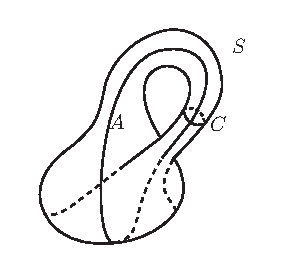
\includegraphics[width=52mm]{figures/2-6-1.pdf}\\图 2.6.1
\end{minipage}\hfill
\begin{minipage}{.47\textwidth}\centering
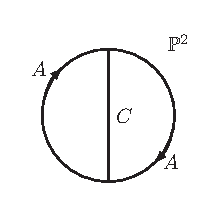
\includegraphics[width=41mm]{figures/2-6-2.pdf}\\图 2.6.2
\end{minipage}
\end{center}
\item 判定是否存在从环面到图 2.6.3 中管状区域 $A$、圆盘 $B$、圆周 $C$ 的收缩映射。
\begin{center}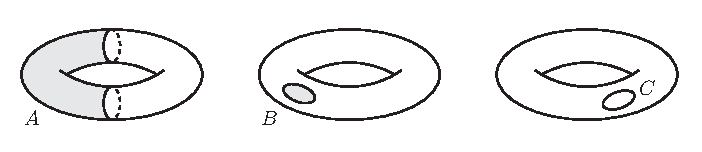
\includegraphics[width=122mm]{figures/2-6-3.pdf}\\图 2.6.3\end{center}
\item 确定所有存在从圆周 $C$ 到它的收缩映射的空间 $X$。
\end{enumerate}

\section{同伦映射诱导的同态}
\sourcepage{121}
现在研究重要的同伦概念。本节始终以 $I$ 表示闭单位区间 $[0,1]$。

\entry{定义}{2.7.1}设 $X,Y$ 为拓扑空间。若存在连续映射 $F:X\times I\to Y$，使对所有 $x\in X$ 有 $F(x,0)=h(x)$、$F(x,1)=k(x)$，则称连续映射 $h,k:X\to Y$ \textbf{同伦}，记为 $h\simeq k$。称 $F$ 为从 $h$ 到 $k$ 的\textbf{同伦}。\translatornote{原文首次写映射时用小写 $f$，随后均用 $F$；这里统一为 $F$。}

可以把 $F$ 看作一种方法，使 $t$ 从 $0$ 变到 $1$ 时，$h$ 连续地“变形”为 $k$。

我们将证明：若 $h,k:|K|\to|L|$ 同伦，则诱导的同调同态 $h_*,k_*$ 相同。这将导出重要结果：同调群是空间同伦型的不变量。

\entry{例}{2.7.2}设 $X=S^1$，则 $H_1(X)$ 为无限循环群。选取图 2.7.1 箭头表示的闭链 $z$ 为生成元。令 $T$ 为环面，$h,k:X\to T$ 如图所示。它们显然同伦，因为可以“把 $h$ 沿环推移”，直到与 $k$ 重合。几何上也清楚，闭链 $h_\#(z),k_\#(z)$ 同调。事实上，把环面右半部剖分为三角形并适当定向，得到 $2$ 维链 $d$，满足 $\partial d=h_\#(z)-k_\#(z)$。由于 $z$ 代表生成元，此时有 $h_*=k_*$。
\begin{center}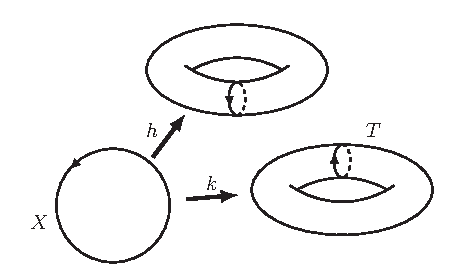
\includegraphics[width=82mm]{figures/2-7-1.pdf}\\图 2.7.1\end{center}
下面证明一般情形。需要两个预备结果。第一个是关于 $|K|\times I$ 的基本拓扑事实，将在下一节证明，见推论 2.8.7：\textit{乘积空间 $|K|\times I$ 的拓扑与子空间族 $\{\sigma\times I:\sigma\in K\}$ 相干。}第二个结果说明 $|K|\times I$ 是多面体。

\sourcepage{122--123}
\entry{引理}{2.7.3}若 $K$ 为复形，则 $|K|\times I$ 是某个复形 $M$ 的多胞体，且对每个 $\sigma\in K$，$\sigma\times I$ 为 $M$ 的某个子复形的多胞体，而 $\sigma\times0$、$\sigma\times1$ 都是 $M$ 的单形。

\noindent\textbf{证明：}对某个 $J$ 有 $|K|\subset E^J$，因而 $|K|\times I\subset E^J\times\R$。用定义重心剖分时的星形构造的一种变形，将它剖分为单形。

对 $p\geq0$，定义
\[
X_p=(|K|\times0)\cup(|K|\times1)\cup(|K^{(p)}|\times I).
\]
归纳剖分 $X_p$。$p=0$ 时，前两项是由各 $\sigma\times0$、$\sigma\times1$ 组成的复形的多胞体；第三项是由各边 $v\times I$ 及其顶点组成的复形的多胞体。它们的并为复形 $M_0$，底空间为 $X_0$。

一般地，假定 $M_{p-1}$ 的底空间为 $X_{p-1}$，并且当 $\dim s<p$ 时，$s\times I$ 为其子复形的多胞体。设 $\dim\sigma=p$，考察
\[
\begin{aligned}
\Bd(\sigma\times I)
&=(\sigma\times I)\setminus(\Int\sigma\times\Int I)\\
&=((\Bd\sigma)\times I)\cup(\sigma\times0)\cup(\sigma\times1).
\end{aligned}
\]
由于 $\Bd\sigma$ 为低维单形的并，这个边界为 $M_{p-1}$ 的子复形 $M_\sigma$ 的多胞体；边界紧致，所以 $M_\sigma$ 有限。令 $w_\sigma=(\widehat\sigma,1/2)$，锥 $w_\sigma*M_\sigma$ 的多胞体为 $\sigma\times I$。它与 $|M_{p-1}|$ 的交为两者某个共同子复形的多胞体。

令 $M_p$ 为 $M_{p-1}$ 与所有这些锥的并，最后令 $M=\bigcup_pM_p$。其底集恰为 $|K|\times I$，还须检验拓扑相同。

乘积拓扑与各 $\sigma\times I$ 相干，而 $|M|$ 的拓扑与其单形相干。若 $C$ 在乘积空间中闭，则 $C\cap(\sigma\times I)$ 在 $\sigma\times I$ 中闭。若 $M$ 的单形 $s$ 位于此乘积内，它是 $\sigma\times I$ 的子空间，因为二者紧致，均有从 $E^J\times\R$ 继承的拓扑。故 $C\cap s$ 在 $s$ 中闭，所以 $C$ 在 $|M|$ 中闭。

反过来，若 $C$ 在 $|M|$ 中闭，则每个 $C\cap s$ 在 $s$ 中闭。$\sigma\times I$ 是有限多个这样的单形的并，因此 $C\cap(\sigma\times I)$ 在 $\sigma\times I$ 中闭。由相干性，$C$ 在 $|K|\times I$ 中闭。\translatornote{原文最后一句误写为“因此 $\sigma$ 在 $|K|\times I$ 中闭”；论证所得应为 $C$ 闭。}\hfill$\square$

\entry{例}{2.7.4}若 $K$ 由一条边及其面组成，上述过程得到图 2.7.2 的剖分。若 $K$ 由一个 $2$ 维单形及其面组成，过程如图 2.7.3：左上为 $|K|\times I$，左下为剖分；右侧将各部分从 $(\widehat\sigma,1/2)$ 沿棱柱五个面的方向分离展示。
\begin{center}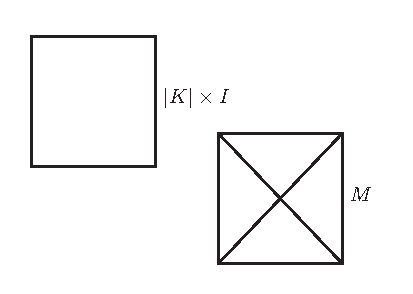
\includegraphics[width=74mm]{figures/2-7-2.pdf}\\图 2.7.2
\medskip

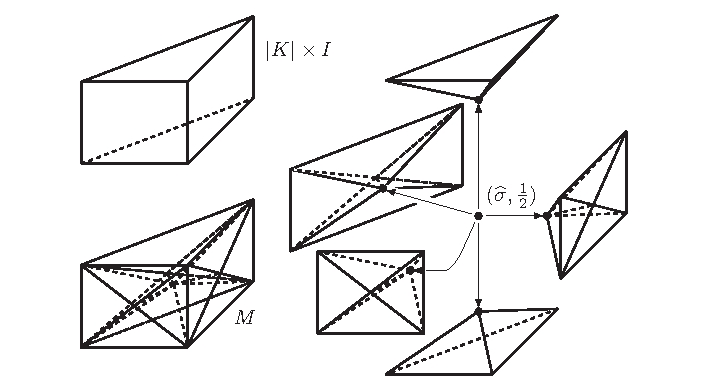
\includegraphics[width=122mm]{figures/2-7-3.pdf}\\图 2.7.3\end{center}

\sourcepage{124--125}
\entry{定理}{2.7.5}若映射 $h,k:|K|\to|L|$ 同伦，则 $h_*,k_*:H_p(K)\to H_p(L)$ 相等。约化同调也如此。

\noindent\textbf{证明：}取前一引理的复形 $M$，底空间为 $|K|\times I$，各 $\sigma\times0$、$\sigma\times1$ 为单形，各 $\sigma\times I$ 为子复形的多胞体。令 $F$ 为从 $h$ 到 $k$ 的同伦，定义 $i(x)=(x,0)$、$j(x)=(x,1)$。则 $i,j:K\to M$ 为单纯映射，且 $Fi=h$、$Fj=k$，见图 2.7.4。
\begin{center}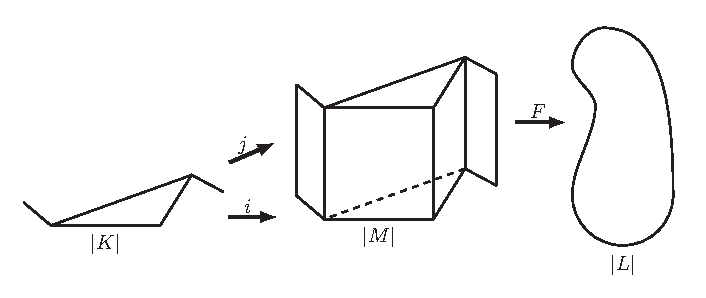
\includegraphics[width=122mm]{figures/2-7-4.pdf}\\图 2.7.4\end{center}
断言 $i_\#,j_\#$ 链同伦。对每个 $\sigma\in K$，令 $\Phi(\sigma)$ 为多胞体等于 $\sigma\times I$ 的子复形。它同胚于闭球，所以无环。面包含关系也保持，故 $\Phi$ 为无环载体，且同时承载 $i_\#,j_\#$。由定理 1.14.10，两链映射链同伦，因此 $i_*=j_*$。故
\[
h_*=F_*i_*=F_*j_*=k_*.
\]\hfill$\square$

结果直接推广到相对同调。若 $h,k:(|K|,|K_0|)\to(|L|,|L_0|)$ 之间存在同伦 $H$，且 $H$ 将 $|K_0|\times I$ 映入 $|L_0|$，则称两者\textbf{作为空间偶的映射同伦}。

\entry{定理}{2.7.6}若 $h,k$ 作为空间偶的映射同伦，则它们在相对同调上诱导相同同态。

\noindent\textbf{证明：}定理 2.7.5 的证明直接适用。$i,j$ 都将 $|K_0|$ 映入 $|K_0|\times I$，它们之间的链同伦也保持相应子复形。因此 $i_*=j_*$ 在相对同调中也成立，其余相同。\hfill$\square$

下面是由乘积拓扑的相干性得到的另一结果，后文将使用。

\entry{定理}{2.7.7}若 $f:K\to L$ 为连续映射 $h:|K|\to|L|$ 的单纯逼近，则 $f$ 同伦于 $h$。

\noindent\textbf{证明：}由引理 2.2.4，$f(x),h(x)$ 位于同一个单形内，所以直线同伦
\[
F(x,t)=(1-t)f(x)+th(x)
\]
将 $|K|\times I$ 映入 $|L|$。若 $L$ 有限，它作为到欧氏空间的映射连续，而 $|L|$ 具有子空间拓扑，所以 $F$ 连续。一般情形只需验证每个 $\sigma\times I$ 上的限制连续。

对 $x\in\sigma$，令 $\tau_x$ 为内部包含 $h(x)$ 的单形。因为 $h(\sigma)$ 紧致，各 $\tau_x$ 只有有限多个，令它们及其面组成 $L_\sigma$。由引理 2.2.4，$f(x)\in\tau_x$，故 $F$ 将 $\{x\}\times I$ 映入 $\tau_x$，于是将 $\sigma\times I$ 映入 $|L_\sigma|$。$L_\sigma$ 有限，其底空间有欧氏子空间拓扑，故此限制连续。再复合连续包含 $|L_\sigma|\to|L|$，得到所需连续性。\hfill$\square$

我们知道同胚空间有同构的同调群。事实上，一种较弱的关系也能保证这一点，即同伦等价。

\entry{定义}{2.7.8}若存在映射 $f:X\to Y$、$g:Y\to X$，使 $gf\simeq i_X$、$fg\simeq i_Y$，则称 $X,Y$ \textbf{同伦等价}（homotopy equivalent），或\textbf{具有相同同伦型}（homotopy type）。$f,g$ 称为\textbf{同伦等价映射}，$g$ 称为 $f$ 的\textbf{同伦逆}。

此关系的对称性、自反性显然，传递性留作习题。因此同伦等价是等价关系。

若 $X$ 与单点空间具有相同同伦型，则称 $X$ \textbf{可缩}（contractible）。这等价于 $i_X$ 同伦于常值映射。例如，单位球可缩，因为 $F(x,t)=(1-t)x$ 是恒等映射到常值映射的同伦。

\sourcepage{126--127}
\entry{定理}{2.7.9}若 $f:|K|\to|L|$ 为同伦等价，则 $f_*$ 为同构。特别地，若 $|K|$ 可缩，则 $K$ 无环。

\noindent\textbf{证明：}若 $g$ 为同伦逆，则 $g_*$ 为 $f_*$ 的逆。\hfill$\square$

一般的同伦等价难以直观描绘，但有一类在几何上较易理解。

\entry{定义}{2.7.10}从 $X$ 到 $A$ 的\textbf{形变收缩}（deformation retraction）是连续映射 $F:X\times I\to X$，满足
\[
\begin{aligned}
F(x,0)&=x&& (x\in X),\\
F(x,1)&\in A&& (x\in X),\\
F(a,t)&=a&& (a\in A,\ t\in I).
\end{aligned}
\]
若存在这样的 $F$，则称 $A$ 为 $X$ 的\textbf{形变收缩核}（deformation retract）。

令 $r(x)=F(x,1)$，则 $r:X\to A$ 为收缩映射。设 $j:A\to X$ 为包含映射，则 $rj=i_A$；而 $F$ 是 $i_X$ 与 $jr$ 之间的同伦，且整个过程中 $A$ 的每一点保持不动。因此 $r,j$ 互为同伦逆。

可以把形变收缩看作逐渐将 $X$ 坍缩到子空间 $A$，同时固定 $A$ 的每一点。这类同伦等价能够几何地描绘。直观上，若 $A$ 为 $X$ 的形变收缩核，$B$ 为 $A$ 的形变收缩核，则 $B$ 为 $X$ 的形变收缩核；这也容易证明。

\entry{定理}{2.7.11}单位球面 $S^{n-1}$ 是去心欧氏空间 $\R^n\setminus\{0\}$ 的形变收缩核。

\noindent\textbf{证明：}令 $X=\R^n\setminus\{0\}$，定义
\[
F(x,t)=(1-t)x+t\frac{x}{\|x\|}.
\]
它将从原点出发的每条开射线收缩到与单位球面的交点，满足要求。\hfill$\square$

\entry{推论}{2.7.12}若 $n\ne m$，则 $\R^n$ 与 $\R^m$ 不同胚。

\noindent\textbf{证明：}若有同胚 $h$，限制后得到 $\R^n\setminus\{0\}$ 与 $\R^m\setminus\{p\}$ 的同胚，其中 $p=h(0)$。后者又同胚于 $\R^m\setminus\{0\}$。由定理，$S^{n-1}$ 与 $S^{m-1}$ 同伦等价。但当 $n\ne m$ 时，前者的 $n-1$ 维约化同调为 $\Z$，后者为零，矛盾。\hfill$\square$

\entry{例}{2.7.13}两个圆周的楔和与字母 $\theta$ 具有相同同伦型。设 $X$ 为图 2.7.5 的平面双孔椭圆区域。左侧箭头说明如何将其坍缩为两个圆周的楔和，右侧说明如何坍缩为 $\theta$。两空间都与 $X$ 同伦等价，因而彼此同伦等价。
\begin{center}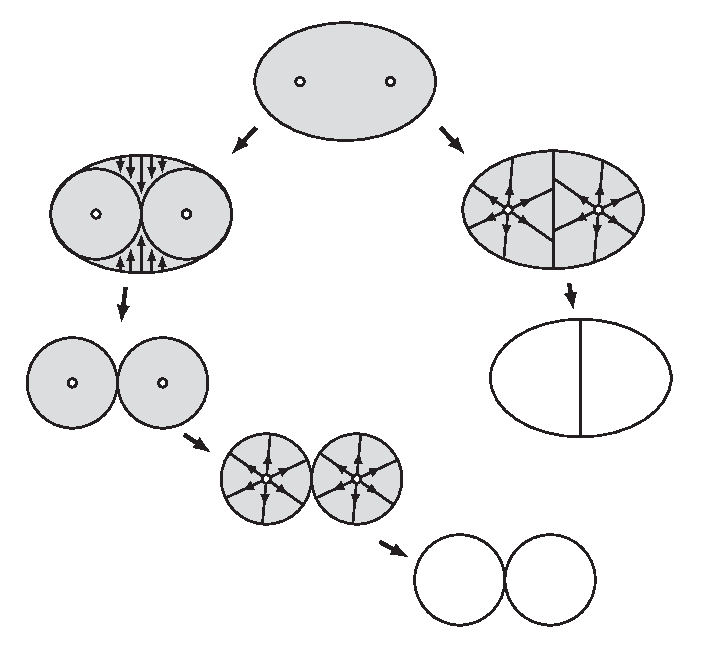
\includegraphics[width=122mm]{figures/2-7-5.pdf}\\图 2.7.5\end{center}

\sourcepage{128--129}
这一情形比乍看更一般。一个有趣事实是，每个同伦等价都能用形变收缩表述。具体地，$X,Y$ 同伦等价，当且仅当存在空间 $Z$ 及嵌入 $h:X\to Z$、$k:Y\to Z$，使 $h(X),k(Y)$ 都是 $Z$ 的形变收缩核，见 [Whi78]、[Fuc71]。\translatornote{本段前后讨论形变收缩，而原文此处写作 homotopy retracts；这里按其所述标准结果译为形变收缩核。}此事实有助于直观理解同伦等价的几何含义。

同伦等价是计算同调群的有力工具。给定复形 $K$，证明其底空间同伦等价于同调已知的空间，通常比直接计算其同调容易。下面的习题说明这一想法。

\subsection*{习题}
\begin{enumerate}
\item 证明同伦等价是任意空间族上的等价关系。
\item 证明：若 $A$ 为 $X$ 的形变收缩核，$B$ 为 $A$ 的形变收缩核，则 $B$ 为 $X$ 的形变收缩核。
\item 将下列空间按同伦等价分类。假定它们都是复形的多胞体，计算各自同调群。
\begin{enumerate}[label=(\alph*)]
\item Möbius 带。
\item 环面。
\item 实心环面 $B^1\times S^1$。\translatornote{原文写 $B^1\times S^1$，但通常实心环面为 $B^2\times S^1$；前者是环带。此处保留原式。}
\item 去掉一点的环面。
\item 去掉两点的环面。
\item 去掉一点的 Klein 瓶。
\item 去掉 $z$ 轴的 $\R^3$。
\item 去掉圆周 $\{x^2+y^2=1,z=0\}$ 的 $\R^3$。
\item (g)、(h) 两空间的交。
\item 从 $S^3$ 中去掉两个相链的圆周。
\item 从 $S^3$ 中去掉两个不相链的圆周。
\end{enumerate}
\item 证明：若 $\dim K=n$，则 $|K|$ 的覆盖维数至少为 $n$。
\item 不使用 $|K|\times I$ 是复形底空间这一事实，按下列步骤证明定理 2.7.5：
\begin{enumerate}[label=(\alph*)]
\item 设 $K,L$ 有限，$h:|K|\to|L|$。证明存在 $\epsilon>0$，使只要 $k$ 对每个 $x$ 满足 $|h(x)-k(x)|<\epsilon$，就有 $h_*=k_*$。［提示：选择 $K'$，使 $h(\overline{\operatorname{St}(v,K')})\subset\operatorname{St}(w,L)$。$\epsilon$ 足够小时，把 $h$ 换为 $k$ 仍成立。］
\item 证明 $K,L$ 有限时的定理。
\item 证明一般情形。［提示：每条闭链都由有限子复形承载。］
\end{enumerate}
\end{enumerate}

\section{商空间回顾}
\sourcepage{129--130}
本节复习商空间的一些基本概念。

若满射 $p:X\to Y$ 满足：$U\subset Y$ 为开集，当且仅当 $p^{-1}(U)$ 在 $X$ 中开，则称为\textbf{商映射}（quotient map）。等价地，也可要求 $E$ 在 $Y$ 中闭，当且仅当 $p^{-1}(E)$ 在 $X$ 中闭。

若 $X$ 的子集 $C$ 等于某个 $A\subset Y$ 的完整原像 $p^{-1}(A)$，则称 $C$ 关于 $p$ \textbf{饱和}（saturated）。$p$ 为商映射，等价于 $p$ 连续，并把饱和开集映为开集；也等价于把饱和闭集映为闭集。

若连续满射 $p$ 为开映射或闭映射，则它为商映射。特别地，若 $X$ 紧致、$Y$ 为 Hausdorff 空间，则 $p$ 为闭映射，因而是商映射。

先列出若干初等事实，证明直接，留给读者。
\begin{itemize}
\item 一一的商映射为同胚。
\item 商映射的复合仍为商映射。
\item 商映射的限制有时仍为商映射：若 $A\subset X$ 饱和，且在 $X$ 中开或闭，则 $p$ 在 $A$ 上的限制为商映射。
\end{itemize}
商映射与连续映射的关系如下：若 $p:X\to Y$ 为商映射，$f:X\to Z$ 连续，且在每个纤维 $p^{-1}(y)$ 上为常值，则存在唯一连续映射 $g:Y\to Z$，使 $gp=f$。称 $g$ 为 $f$ \textbf{诱导的映射}。

如下定义商空间。设 $X^*$ 为将 $X$ 分成两两不交子集的一个划分，令 $\pi:X\to X^*$ 将每点映到包含它的那个子集。规定 $U\subset X^*$ 为开集，当且仅当 $\pi^{-1}(U)$ 在 $X$ 中开，得到 $X^*$ 上的拓扑。此时 $\pi$ 为商映射，称 $X^*$ 为 $X$ 的\textbf{商空间}。常说它由将划分中的每个成员等同为一点而得到。

若 $p:X\to Y$ 为商映射，可按如下方式把 $Y$ 视为 $X$ 的商空间：用各纤维 $p^{-1}(y)$ 划分 $X$，所得 $X^*$ 与 $Y$ 同胚。事实上，利用前面的诱导映射性质，分别得到 $g:X^*\to Y$、$h:Y\to X^*$，满足 $g\pi=p$、$hp=\pi$；容易看出它们互逆。

\entry{例}{2.8.1}将 $x$-$z$ 平面内以 $(2,0,0)$ 为中心的单位圆绕 $z$ 轴旋转，得到 $\R^3$ 的子空间 $X$。用柱坐标 $(r,\theta,z)$，它由方程 $(r-2)^2+z^2=1$ 表示。令 $I^2=I\times I$，对 $(s,t)\in I^2$，按
\[
r-2=\cos2\pi t,\qquad z=\sin2\pi t,\qquad\theta=2\pi s
\]
定义 $p:I^2\to X$。可验证它为满的闭商映射。因此 $X$ 可视为将 $(s,0)$ 与 $(s,1)$、$(0,t)$ 与 $(1,t)$ 分别等同而得的商空间，见图 2.8.1。这是第 1.4 节粘合矩形各边构造环面的拓扑表述。
\begin{center}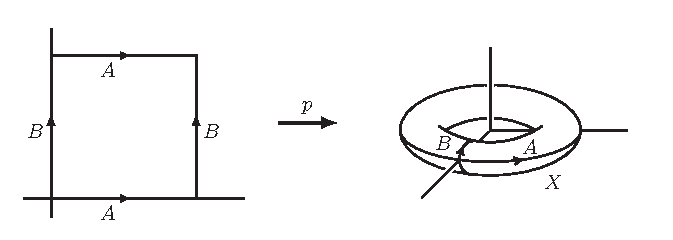
\includegraphics[width=117mm]{figures/2-8-1.pdf}\\图 2.8.1\end{center}

\sourcepage{131--132}
分离公理在商空间中不一定保持，例如 Hausdorff 空间的商空间未必 Hausdorff。一般只能说：若每个纤维 $p^{-1}(y)$ 都在 $X$ 中闭，则 $Y$ 为 $T_1$ 空间，即单点集闭。因此，若 $X^*$ 是将 $X$ 划分为闭集的划分，所得商空间为 $T_1$ 空间。\translatornote{原文还插入一句“若 $X$ 为 Hausdorff，则 $Y$ 的单点集闭”；单有该假设不足，仍须保留纤维闭的条件。}

后面会更详细地讨论商空间的分离公理。这里最后讨论：两个商映射的笛卡尔积何时仍为商映射？有两个相关结果。

\entry{定理}{2.8.2}若 $p:X\to Y$ 为商映射，$C$ 为局部紧致 Hausdorff 空间，则 $p\times i_C:X\times C\to Y\times C$ 为商映射。

\noindent\textbf{证明：}令 $\pi=p\times i_C$。设 $A\subset Y\times C$ 且 $\pi^{-1}(A)$ 开，证明 $A$ 开。给定 $(y_0,c_0)\in A$，选 $x_0$ 使 $p(x_0)=y_0$。可选择 $x_0,c_0$ 的开邻域 $U_1,W$，使 $U_1\times W\subset\pi^{-1}(A)$。由局部紧致 Hausdorff 性，选 $c_0$ 的开邻域 $V$，使 $\overline V$ 紧致且 $\overline V\subset W$。于是
\[
U_1\times\overline V\subset\pi^{-1}(A).
\]
一般地，若已构造开邻域 $U_i$，使 $U_i\times\overline V\subset\pi^{-1}(A)$，则 $p^{-1}p(U_i)$ 虽未必开，却包含 $U_i$。构造开集 $U_{i+1}$，使
\[
p^{-1}p(U_i)\times\overline V\subset U_{i+1}\times\overline V\subset\pi^{-1}(A).
\]
对每个 $x\in p^{-1}p(U_i)$，有 $\{x\}\times\overline V\subset\pi^{-1}(A)$。由紧致性，可取开邻域 $W_x$，使 $W_x\times\overline V\subset\pi^{-1}(A)$。令 $U_{i+1}=\bigcup_xW_x$ 即可，见图 2.8.2。
\begin{center}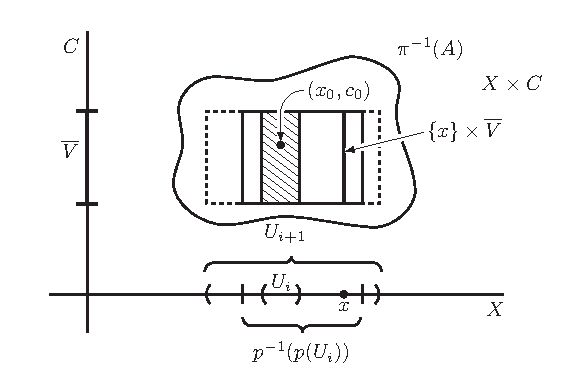
\includegraphics[width=103mm]{figures/2-8-2.pdf}\\图 2.8.2\end{center}
最后令 $U=\bigcup_iU_i$。它开，$U\times V$ 是 $(x_0,c_0)$ 的邻域，并包含于 $\pi^{-1}(A)$。此外，
\[
U\subset p^{-1}p(U)=\bigcup_i p^{-1}p(U_i)=\bigcup_iU_{i+1}=U,
\]
故 $U$ 饱和，$p(U)$ 在 $Y$ 中开。于是 $p(U)\times V=\pi(U\times V)\subset A$ 是 $(y_0,c_0)$ 的开邻域，证毕。\hfill$\square$

\entry{推论}{2.8.3}若 $p:A\to B$、$q:C\to D$ 为商映射，且 $p$ 的定义域 $A$ 与 $q$ 的值域 $D$ 均为局部紧致 Hausdorff 空间，则 $p\times q:A\times C\to B\times D$ 为商映射。

\noindent\textbf{证明：}写成复合 $A\times C\xrightarrow{i_A\times q}A\times D\xrightarrow{p\times i_D}B\times D$，两映射均为商映射，复合亦然。\hfill$\square$

相干拓扑与商映射有密切关系，描述如下。

\sourcepage{133}
\entry{定义}{2.8.4}设空间 $E$ 是两两不交子空间 $E_\alpha$ 的并，且每个 $E_\alpha$ 在 $E$ 中开且闭，则称 $E$ 为它们的\textbf{拓扑和}（topological sum），记为 $E=\coprod E_\alpha$。集合 $U$ 在 $E$ 中开，当且仅当每个 $U\cap E_\alpha$ 在 $E_\alpha$ 中开。

更一般地，对未必互不相交的空间族 $\{X_\alpha\}_{\alpha\in J}$，令 $E_\alpha=X_\alpha\times\{\alpha\}$，以这些不交空间的并为底集，赋予上述拓扑。存在自然投影 $p:E\to\bigcup X_\alpha$，把每个 $X_\alpha\times\{\alpha\}$ 投影到 $X_\alpha$。有时也称 $E$ 为各 $X_\alpha$ 的拓扑和。

\entry{引理}{2.8.5}设 $X$ 为若干子空间 $X_\alpha$ 的并，$E$ 为其拓扑和，$p:E\to X$ 为自然投影。则 $X$ 的拓扑与各 $X_\alpha$ 相干，当且仅当 $p$ 为商映射。

证明立即得到。在此情形，常称 $X$ 为各 $X_\alpha$ 的\textbf{相干并}。

\entry{定理}{2.8.6}若 $X$ 的拓扑与子空间族 $X_\alpha$ 相干，$Y$ 为局部紧致 Hausdorff 空间，则 $X\times Y$ 的拓扑与各 $X_\alpha\times Y$ 相干。

\noindent\textbf{证明：}令 $E=\coprod(X_\alpha\times\{\alpha\})$，$p:E\to X$ 为投影。由前一定理，$p\times i_Y:E\times Y\to X\times Y$ 为商映射。由于 $E$ 为各 $E_\alpha$ 的拓扑和，$E\times Y$ 是各开子空间 $E_\alpha\times Y$ 的不交并，因此为它们的拓扑和。应用引理即得结论。\hfill$\square$

\entry{推论}{2.8.7}$|K|\times I$ 的拓扑与各 $\sigma\times I$（$\sigma\in K$）相干。

\noindent\textbf{证明：}$|K|$ 按定义与其单形相干，而 $I$ 是局部紧致 Hausdorff 空间，事实上紧致，故可用定理。\hfill$\square$

\sourcepage{134--135}
\entry{推论}{2.8.8}若 $w*K$ 为锥，则映射 $\pi:|K|\times I\to|w*K|$，$\pi(x,t)=(1-t)x+tw$，为商映射。它将 $|K|\times\{1\}$ 压缩为点 $w$，其他地方为一一映射。\translatornote{原文此处把被压缩的子集误印为整个 $|K|\times I$。}

\noindent\textbf{证明：}若 $\sigma=v_0\cdots v_n$，以 $w*\sigma$ 表示单形 $wv_0\cdots v_n$。集合在锥中闭，当且仅当与每个 $w*\sigma$ 的交闭；集合在乘积中闭，当且仅当与每个 $\sigma\times I$ 的交闭。因此只需证明限制 $\pi':\sigma\times I\to w*\sigma$ 为商映射。它连续满射，涉及的空间均紧致 Hausdorff，所以成立。\hfill$\square$

此推论启发我们定义任意拓扑空间上的锥。

\entry{定义}{2.8.9}空间 $X$ 上的\textbf{锥} $C(X)$，定义为将 $X\times I$ 的子集 $X\times\{1\}$ 等同为一点所得商空间，此点称为\textbf{锥顶}。形式上，将 $X\times I$ 划分为 $t<1$ 时的各单点集 $\{(x,t)\}$ 与集合 $X\times\{1\}$，取所得商空间。

以下定义用于习题 2。

\entry{定义}{2.8.10}取 $\R^2$ 的两个副本 $\R^2\times\{a\}$、$\R^2\times\{b\}$，当 $x\ne0$ 时等同 $(x,a)$ 与 $(x,b)$，得到的空间称为\textbf{双原点平面}（plane with two origins）。

\subsection*{习题}
\begin{enumerate}
\item 验证本节未证明的商空间结果。
\item \begin{enumerate}[label=(\alph*)]
\item 证明双原点平面的每点都有与 $\R^2$ 某开子集同胚的邻域。
\item 证明双原点平面不是 Hausdorff 空间。
\end{enumerate}
\item \begin{enumerate}[label=(\alph*)]
\item 若 $p:X\to Y$ 为开商映射，$A$ 在 $X$ 中开，证明 $p|_A:A\to p(A)$ 为开商映射。
\item 将“开”换为“闭”，重复 (a)。
\end{enumerate}
\item 若 $p:A\to B$、$q:C\to D$ 为开商映射，证明 $p\times q$ 也是。
\item 若 $X$ 为各 $X_\alpha$ 的相干并，$Y$ 为 $X$ 的开或闭子空间，证明 $Y$ 为各 $X_\alpha\cap Y$ 的相干并。
\item 设 $K,L$ 为复形，$K$ 局部有限，证明 $|K|\times|L|$ 的拓扑与各 $\sigma\times\tau$（$\sigma\in K,\tau\in L$）相干。
\item 证明商映射的拓扑和仍为商映射。
\end{enumerate}

\section{\texorpdfstring{$*$}{*}应用：球面映射}
\sourcepage{135--136}
本节给出同调论对几何与拓扑经典问题的若干应用。下一节的著名 Lefschetz 不动点定理将推广这里的结果。

\entry{定义}{2.9.1}设 $n\geq1$，$f:S^n\to S^n$ 连续。若 $\alpha$ 为无限循环群 $H_n(S^n)$ 的两个生成元之一，则对某个整数 $d$，$f_*(\alpha)=d\alpha$。因为 $f_*(-\alpha)=d(-\alpha)$，$d$ 与生成元选择无关，称为 $f$ 的\textbf{映射度}（degree），记为 $\deg f$。

\entry{引理}{2.9.2}映射度满足：
\begin{enumerate}[label=(\arabic*)]
\item 若 $f\simeq g$，则 $\deg f=\deg g$。
\item 若 $f$ 能扩张为连续映射 $\widehat f:B^{n+1}\to S^n$，则 $\deg f=0$。
\item 恒等映射的映射度为 $1$。
\item $\deg(f\circ g)=(\deg f)(\deg g)$。
\end{enumerate}
\noindent\textbf{证明：}(1) 由定理 2.7.5。(2) 中 $f_*$ 为复合
\[
H_n(S^n)\xrightarrow{j_*}H_n(B^{n+1})\xrightarrow{\widehat f_*}H_n(S^n),
\]
其中 $j$ 为包含。球无环，所以复合为零。(3)、(4) 直接由定理 2.6.2 得到。\hfill$\square$

\entry{定理}{2.9.3}不存在收缩映射 $r:B^{n+1}\to S^n$。

\noindent\textbf{证明：}恒等映射的映射度为 $1$。若有收缩映射，它就是恒等映射到球的扩张，由引理 (2)，恒等映射的度又为 $0$，矛盾。\hfill$\square$

\entry{定理}{2.9.4（Brouwer 不动点定理）}若 $\varphi:B^n\to B^n$ 连续，则存在 $x\in B^n$，使 $\varphi(x)=x$。

\noindent\textbf{证明：}假设没有不动点，则可定义
\[
h:B^n\to S^{n-1},\qquad h(x)=\frac{x-\varphi(x)}{\|x-\varphi(x)\|}.
\]
令 $f$ 为其在边界球面上的限制，由引理 (2)，$\deg f=0$。另一方面，定义
\[
H(u,t)=\frac{u-t\varphi(u)}{\|u-t\varphi(u)\|}.
\]
当 $t=1$ 时，分母由无不动点假设非零；当 $t<1$ 时，$\|u\|=1$，而 $\|t\varphi(u)\|\leq t<1$，分母仍非零。此同伦连接恒等映射和 $f$，故 $\deg f=1$，矛盾。\translatornote{由于前面只对正维球面定义映射度，此证明直接适用于 $n\geq2$；$n=1$ 可由介值定理证明，$n=0$ 平凡。}\hfill$\square$

\entry{定义}{2.9.5}\textbf{对径映射}（antipodal map）$a:S^n\to S^n$ 定义为 $a(x)=-x$。

后续应用需要证明其映射度为 $(-1)^{n+1}$。这里给直接证明，下一节及第 4.4 节还会给出其他证明。关键是下面的引理。

\entry{引理}{2.9.6}反射映射 $\rho:S^n\to S^n$，
\[
\rho(x_1,\ldots,x_n,x_{n+1})=(x_1,\ldots,x_n,-x_{n+1}),
\]
的映射度为 $-1$。

反射在球面每点处反转切平面的定向，这或许直观清楚，但仍须依定义 2.9.1 证明。先定义所需的三角剖分。

\sourcepage{137--138}
\entry{定义}{2.9.7}空间 $X$ 的一个\textbf{三角剖分}（triangulation）是复形 $L$ 连同同胚 $h:|L|\to X$。若存在这样的剖分，称 $X$ \textbf{可三角剖分}（triangulable）。

\noindent\textbf{引理 2.9.6 的证明：第一步。}构造 $S^n$ 的 $n$ 维三角剖分，使反射对应于该复形到自身的单纯映射。

设有限复形 $K\subset\R^N\times\{0\}$，取 $w_0=(0,\ldots,0,1)$、$w_1=(0,\ldots,0,-1)$，令悬挂 $S(K)=(w_0*K)\cup(w_1*K)$。令 $r$ 交换两个锥顶并固定 $K$ 的各顶点。要构造 $n-1$ 维复形 $K$ 及同胚 $k:|S(K)|\to S^n$，使 $\rho k=kr$。

取 $S^{n-1}$ 的任意 $n-1$ 维三角剖分 $h:|K|\to S^{n-1}$。若 $y=(1-t)x+tw_0$，定义 $k(y)=(\sqrt{1-t^2}\,h(x),t)$；若 $y=(1-t)x+tw_1$，定义 $k(y)=(\sqrt{1-t^2}\,h(x),-t)$，见图 2.9.1。
\begin{center}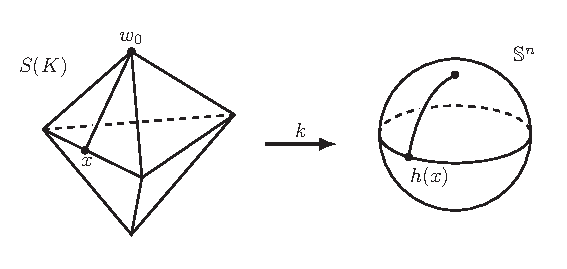
\includegraphics[width=101mm]{figures/2-9-1.pdf}\\图 2.9.1\end{center}
容易验证 $k$ 为同胚。又因为 $r((1-t)x+tw_0)=(1-t)x+tw_1$，所以 $\rho k=kr$。

\textbf{第二步。}只需证明 $r$ 对最高维同调作用为乘以 $-1$。设 $z$ 为 $S(K)$ 的 $n$ 维闭链，因 $\dim K=n-1=m$，可写成 $z=[w_0,c_m]+[w_1,d_m]$。若 $n>1$，
\[
0=\partial z=c_m-[w_0,\partial c_m]+d_m-[w_1,\partial d_m].
\]
限制到 $K$ 得 $c_m+d_m=0$，故 $z=[w_0,c_m]-[w_1,c_m]$。于是 $r_\#z=[w_1,c_m]-[w_0,c_m]=-z$。$n=1$ 的计算类似。\hfill$\square$

\entry{定理}{2.9.8}对 $n\geq1$，对径映射的映射度为 $(-1)^{n+1}$。

\noindent\textbf{证明：}任意坐标反射 $\rho_i$ 的度也为 $-1$。事实上，交换第 $i$、第 $n+1$ 坐标的同胚 $h$ 满足 $\rho_i=h^{-1}\rho h$，所以
\[
\deg\rho_i=(\deg h^{-1})(\deg\rho)(\deg h)
=\deg(h^{-1}h)\deg\rho=-1.
\]
而 $a=\rho_1\rho_2\cdots\rho_{n+1}$，故得到结论。\hfill$\square$

\entry{定理}{2.9.9}若 $h:S^n\to S^n$ 的映射度不等于 $(-1)^{n+1}$，则它有不动点。

\noindent\textbf{证明：}反设没有不动点。将 $h(x)$ 沿最短大圆弧移动到 $-x$，得到 $h\simeq a$，故度为 $(-1)^{n+1}$，矛盾。具体同伦为
\[
H(x,t)=\frac{(1-t)h(x)-tx}{\|(1-t)h(x)-tx\|}.
\]
若分母为零，则 $(1-t)h(x)=tx$，取范数得 $1-t=t$，即 $t=1/2$，进而 $h(x)=x$，矛盾。\hfill$\square$

\sourcepage{139}
\entry{定理}{2.9.10}若 $h:S^n\to S^n$ 的度不等于 $1$，则它将某点映到该点的对径点。

\noindent\textbf{证明：}$ah$ 的度不等于 $(-1)^{n+1}$，故有不动点 $x$。于是 $a(h(x))=x$，即 $h(x)=-x$。\hfill$\square$

\entry{推论}{2.9.11}球面 $S^n$ 存在处处非零的切向量场，当且仅当 $n$ 为奇数。

\noindent\textbf{证明：}若 $n=2k-1$，对 $x\in S^n\subset\R^{2k}$ 定义
\[
v(x)=(-x_2,x_1,-x_4,x_3,\ldots,-x_{2k},x_{2k-1}).
\]
它与 $x$ 垂直，故切于球面，且 $\|v(x)\|=\|x\|=1$，处处非零。

反过来，若有处处非零的切向量场 $w$，则 $h(x)=w(x)/\|w(x)\|$ 为球面到自身的映射。因 $w(x)\perp x$，既不可能 $h(x)=x$，也不可能 $h(x)=-x$。由定理 2.9.9、2.9.10，分别得 $\deg h=(-1)^{n+1}$ 和 $\deg h=1$，故 $n$ 为奇数。\hfill$\square$

习题 2 要求证明代数基本定理，为完整起见陈述如下。

\entry{定理}{2.9.12（代数基本定理）}每个实或复系数多项式 $z^n+a_{n-1}z^{n-1}+\cdots+a_1z+a_0$（$n\geq1$）在复平面中都有根。

\sourcepage{140--141}
\subsection*{习题}
\begin{enumerate}
\item \begin{enumerate}[label=(\alph*)]
\item 设 $K$ 为图 2.9.2 的正方形边界复形，$\operatorname{sd}K$ 为第一次重心剖分。单纯映射 $f:\operatorname{sd}K\to K$ 由 $f(a_i)=a_{2i}$ 给定，下标必要时模 $8$。证明其映射度为 $2$。
\begin{center}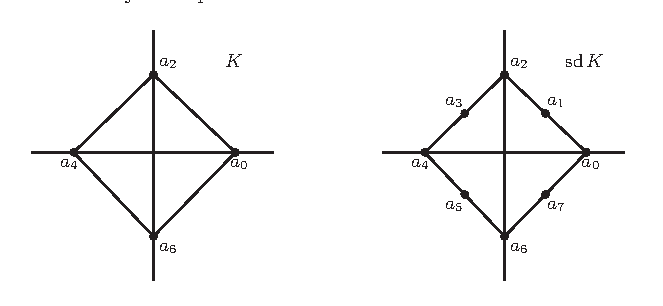
\includegraphics[width=117mm]{figures/2-9-2.pdf}\\图 2.9.2\end{center}
\item 将 $S^1$ 视为单位模复数集，证明 $h(z)=z^2$ 的度为 $2$。［提示：通过径向投影，它给出 $|K|$ 到自身的映射，与 (a) 的 $f$ 同伦。］
\item 对任意正整数 $n$，证明 $k(z)=z^n$ 的度为 $n$。
\end{enumerate}
\item 用习题 1 按下列步骤证明代数基本定理。令 $S_c$ 为复平面中圆周 $|z|=c$。假定给定多项式在闭圆盘 $|z|\leq c$ 中没有根，定义 $h:S_c\to\mathbb C\setminus\{0\}$ 为 $h(z)=z^n+a_{n-1}z^{n-1}+\cdots+a_0$。
\begin{enumerate}[label=(\alph*)]
\item 证明 $h_*$ 为零同态。
\item 证明当 $c$ 足够大时，$h$ 同伦于 $k(z)=z^n$。［提示：取 $F(z,t)=z^n+t(a_{n-1}z^{n-1}+\cdots+a_0)$。］
\item 导出矛盾。
\end{enumerate}
\item 按下列步骤证明反射映射引理证明中第一步的 $k$ 为同胚。\translatornote{原文误引为定理 2.9.8 的证明，实际在引理 2.9.6 的证明中。}
\begin{enumerate}[label=(\alph*)]
\item 证明映射 $p:|K|\times[-1,1]\to|S(K)|$ 与 $q:|K|\times[-1,1]\to S^n$ 均为商映射，其中
\[
p(x,t)=\begin{cases}(1-t)x+tw_0,&t\geq0,\\(1+t)x-tw_1,&t<0,\end{cases}
\qquad q(x,t)=(\sqrt{1-t^2}\,h(x),t).
\]
\item 证明 $p,q$ 诱导同胚 $k$。
\end{enumerate}
\item 证明习题 1(c) 对 $n\leq0$ 的整数也成立。
\item 参照习题 1(b)，设 $m$ 为任意复常数，证明函数 $f(z)=(z+m)^2$ 的度为 $2$。［提示：用同伦论证。］\translatornote{原题未说明此函数的定义域和值域。它一般不是 $S^1\to S^1$ 的映射；若理解为在充分大圆周上归一化所得的圆周映射，其度为 $2$。不能对任意 $m$ 直接在单位圆周上使用这一断言。}
\end{enumerate}

\section{\texorpdfstring{$*$}{*}Lefschetz 不动点定理}
\sourcepage{141--142}
前面的不动点定理讨论球面、球到自身的映射。Solomon Lefschetz 作出了广泛推广，使其适用于更一般的拓扑空间。本节证明这个定理。

先复习代数知识。方阵 $A=(a_{ij})$ 的\textbf{迹}（trace）定义为 $\operatorname{tr}A=\sum_{j=1}^n a_{jj}$。若 $A,B$ 都是 $n$ 阶方阵，则
\[
\operatorname{tr}(AB)=\sum_{i,j}a_{ij}b_{ji}=\operatorname{tr}(BA).
\]
若 $G$ 为基为 $e_1,\ldots,e_n$ 的自由阿贝尔群，$\varphi:G\to G$ 为同态，则定义其迹为相应矩阵的迹。它与基选择无关，因为另一组基下的矩阵为 $B^{-1}AB$，而 $\operatorname{tr}(B^{-1}(AB))=\operatorname{tr}((AB)B^{-1})=\operatorname{tr}A$。同样，若 $i$ 为同构，则 $\operatorname{tr}(i\varphi i^{-1})=\operatorname{tr}\varphi$。

设 $K$ 为有限复形，$\varphi$ 为其链复形到自身的链映射。各 $C_p(K)$ 自由有限秩，故可定义 $\operatorname{tr}(\varphi,C_p(K))$。$H_p(K)$ 不一定自由，但除去挠子群 $T_p(K)$ 后得到自由群，且 $\varphi_*$ 诱导此商群到自身的同态。以 $\operatorname{tr}(\varphi_*,H_p(K)/T_p(K))$ 表示其迹。这两个迹之间没有明显关系，所以下式相当引人注目。

\entry{定理}{2.10.1（Hopf 迹定理）}若 $K$ 为有限复形，$\varphi$ 为链映射，则
\[
\sum_p(-1)^p\operatorname{tr}(\varphi,C_p(K))
=\sum_p(-1)^p\operatorname{tr}(\varphi_*,H_p(K)/T_p(K)).
\]
\noindent\textbf{证明：第一步。}设 $G$ 自由有限秩，$H$ 为子群，且 $G/H$ 自由。若 $\varphi:G\to G$ 保持 $H$，证明
\[
\operatorname{tr}(\varphi,G)=\operatorname{tr}(\varphi',G/H)+\operatorname{tr}(\varphi'',H),
\]
其中 $\varphi',\varphi''$ 为诱导同态。选取 $G/H$ 的基 $\alpha_1+H,\ldots,\alpha_n+H$ 和 $H$ 的基 $\beta_1,\ldots,\beta_p$。若相应矩阵为 $A,B$，则
\[
\varphi'(\alpha_j+H)=\sum_i a_{ij}(\alpha_i+H),\qquad
\varphi''(\beta_j)=\sum_i b_{ij}\beta_i.
\]
$\alpha_1,\ldots,\alpha_n,\beta_1,\ldots,\beta_p$ 为 $G$ 的基，且 $\varphi(\alpha_j)=\sum_i a_{ij}\alpha_i+H\text{ 中某元素}$，$\varphi(\beta_j)=\sum_i b_{ij}\beta_i$。因此矩阵为
\[
\begin{pmatrix}A&0\\ *&B\end{pmatrix},
\]
其迹为 $\operatorname{tr}A+\operatorname{tr}B$。

\sourcepage{143--144}
\textbf{第二步。}仍以 $C_p,Z_p,B_p,W_p$ 表示链群、闭链群、边界群和弱边界群，有 $B_p\subset W_p\subset Z_p\subset C_p$。$\varphi$ 为链映射，保持这些群。将证明 $C_p/Z_p$ 与 $Z_p/W_p$ 自由，由第一步即得
\[
\operatorname{tr}(\varphi,C_p)=\operatorname{tr}(\varphi,C_p/Z_p)
+\operatorname{tr}(\varphi,Z_p/W_p)+\operatorname{tr}(\varphi,W_p).\tag{i}
\]
这里省略区分各诱导同态的撇号。

\textbf{第三步。}限制边界算子的值域，得到满同态 $C_p\to B_{p-1}$，核为 $Z_p$，故诱导同构 $C_p/Z_p\cong B_{p-1}$。后者自由，前者也自由。由于 $\varphi$ 与边界可交换，此同构与 $\varphi$ 可交换，所以
\[
\operatorname{tr}(\varphi,C_p/Z_p)=\operatorname{tr}(\varphi,B_{p-1}).\tag{ii}
\]
\textbf{第四步。}自然投影的复合 $Z_p\to Z_p/B_p=H_p\to H_p/T_p$ 为满射，核为 $W_p$，因此诱导同构 $Z_p/W_p\cong H_p/T_p$，所以前者自由。各投影与 $\varphi$ 可交换，故
\[
\operatorname{tr}(\varphi,Z_p/W_p)=\operatorname{tr}(\varphi_*,H_p/T_p).\tag{iii}
\]
\textbf{第五步。}证明
\[
\operatorname{tr}(\varphi,W_p)=\operatorname{tr}(\varphi,B_p).\tag{iv}
\]
由自由阿贝尔群基本定理，可选 $W_p$ 的基 $\alpha_1,\ldots,\alpha_n$，使 $B_p$ 有基 $m_1\alpha_1,\ldots,m_k\alpha_k$，其中 $m_i\geq1$。因为 $W_p/B_p$ 为挠群，所以 $k=n$。写作
\[
\varphi(\alpha_j)=\sum_i a_{ij}\alpha_i,\qquad
\varphi(m_j\alpha_j)=\sum_i b_{ij}(m_i\alpha_i).
\]
将前式乘以 $m_j$，比较得 $m_ja_{ij}=b_{ij}m_i$。特别地，$a_{ii}=b_{ii}$，两迹相等。

\textbf{第六步。}将 (ii)--(iv) 代入 (i)，得到
\[
\operatorname{tr}(\varphi,C_p)=\operatorname{tr}(\varphi,B_{p-1})
+\operatorname{tr}(\varphi_*,H_p/T_p)+\operatorname{tr}(\varphi,B_p).
\]
乘以 $(-1)^p$ 并对 $p$ 求和，右边第一、第三项两两抵消，即得结论。\hfill$\square$

\entry{定义}{2.10.2}有限复形 $K$ 的\textbf{Euler 数}（Euler number）经典地定义为
\[
\chi(K)=\sum_p(-1)^p\operatorname{rank}C_p(K),
\]
即各维单形数目的交错和。

\entry{定理}{2.10.3}设 $\beta_p=\operatorname{rank}(H_p(K)/T_p(K))$ 为 $p$ 维 Betti 数，则 $\chi(K)=\sum_p(-1)^p\beta_p$。

\noindent\textbf{证明：}对恒等链映射用 Hopf 迹定理。它在链群上的迹为链群的秩，在同调自由商群上的迹为 $\beta_p$。\hfill$\square$

因此 Euler 数为底空间的拓扑不变量。此定理有许多后果，例如 $\R^3$ 中有界凸开区域的边界同胚于 $S^2$，故 Euler 数为 $2$；由此可证明只有五种正多面体，即经典的五种 Platonic 立体。\translatornote{原文此处没有写出“有界”；要由凸开区域边界得到球面，需有此类限定。}

\sourcepage{145--146}
\entry{定义}{2.10.4}有限复形底空间的连续自映射 $h$ 的 \textbf{Lefschetz 数}定义为
\[
\Lambda(h)=\sum_p(-1)^p\operatorname{tr}(h_*,H_p(K)/T_p(K)).
\]
由定理 2.7.5，它只依赖同伦类。它也只依赖底空间，不依赖具体复形：若 $|L|=|K|$，恒等映射诱导同构 $j_*:H_p(L)\to H_p(K)$，而 $(h_L)_*=j_*^{-1}(h_K)_*j_*$，两者的迹相同。

\entry{定理}{2.10.5（Lefschetz 不动点定理）}若 $K$ 为有限复形，$h:|K|\to|K|$ 连续，且 $\Lambda(h)\ne0$，则 $h$ 有不动点。

\noindent\textbf{证明：}假设没有不动点，证明 $\Lambda(h)=0$。

\textbf{第一步。}可假定每个顶点 $v$ 满足
\[
h(\overline{\operatorname{St}(v,K)})\cap\overline{\operatorname{St}(v,K)}=\varnothing.\tag{$*$}
\]
令 $\epsilon=\min_x|x-h(x)|>0$。由一致连续性，选 $\delta>0$，使 $|x-y|<\delta$ 时 $|h(x)-h(y)|\leq\epsilon/3$。令 $\lambda=\min\{\delta,\epsilon/2\}$。若 $A$ 的直径小于 $\lambda$，则 $A,h(A)$ 的直径均小于 $\epsilon/2$，故必不相交。将 $K$ 换成各闭星形邻域直径小于 $\lambda$ 的剖分，$(*)$ 即成立，且 $\Lambda(h)$ 不变。

\textbf{第二步。}选剖分 $K'$，使 $h$ 有单纯逼近 $f:K'\to K$。若 $s\in K'$、$\sigma\in K$ 且 $s\subset\sigma$，断言 $f(s)\ne\sigma$。反设相等，取 $s$ 的顶点 $w$，$v=f(w)$ 为 $\sigma$ 的顶点。由 $w\in\sigma$，有 $w\in\overline{\operatorname{St}(v,K)}$，故
\[
h(w)\in h(\overline{\operatorname{St}(v,K)}).
\]
另一方面，单纯逼近条件给出 $h(\operatorname{St}(w,K'))\subset\operatorname{St}(v,K)$，故 $h(w)\in\operatorname{St}(v,K)$，与 $(*)$ 矛盾。

\textbf{第三步。}令 $\lambda:\mathcal C(K)\to\mathcal C(K')$ 为剖分算子，$\varphi=f_\#\lambda$ 诱导 $h_*$。以通常的定向单形为基，考察 $\varphi$ 的矩阵。$\lambda(\sigma)$ 为所有位于 $\sigma$ 内的定向单形 $s$ 的线性组合。由第二步，各 $f(s)$ 均不是 $\sigma$，因此 $\varphi(\sigma)$ 中 $\sigma$ 的系数为零。矩阵所有对角元都为零，故各维迹为零。由 Hopf 迹定理，$\Lambda(h)=\sum_p(-1)^p\operatorname{tr}(\varphi,C_p(K))=0$。\hfill$\square$

为应用此定理，需要下面的引理。

\entry{引理}{2.10.6}若有限复形 $K$ 的底空间连通，则任意连续自映射 $h$ 在 $H_0(K)$ 上诱导恒等映射。

\noindent\textbf{证明：}取单纯逼近 $f:K'\to K$。对顶点 $v$，剖分算子的像由 $v$ 的剖分承载，只能是 $v$ 的整数倍；保持增广迫使 $\lambda(v)=v$。所以 $f_\#\lambda(v)=f_\#(v)$ 为一个顶点，由连通性，它同调于 $v$。故 $h_*$ 为恒等映射。\translatornote{原文证明首句将 $f$ 的目标误写为 $K'$，这里取 $K$。}\hfill$\square$

\entry{定理}{2.10.7}若有限复形底空间无环，则其每个连续自映射都有不动点。

\noindent\textbf{证明：}$H_0(K)\cong\Z$，且其上 $h_*$ 为恒等映射，迹为 $1$。高维同调为零，故 $\Lambda(h)=1$，定理适用。\hfill$\square$

\sourcepage{147--149}
\entry{定理}{2.10.8}对径映射 $a:S^n\to S^n$ 的度为 $(-1)^{n+1}$。

\noindent\textbf{证明：}若 $h$ 的度为 $d$，则零维同调上的迹为 $1$，最高维同调上的迹为 $d$，故
\[
\Lambda(h)=1+(-1)^n d.\tag{$\dagger$}
\]
对径映射无不动点，所以 $\Lambda(a)=0$，即 $1+(-1)^n\deg a=0$，得到结论。\hfill$\square$

下列定义用于习题 6。

\entry{定义}{2.10.9}设 $\mathcal B$ 是 $\R^3$ 中的有限多边形族，任意两者至多相交于一条公共边或一个公共顶点。各多边形称为 $\mathcal B$ 的\textbf{面}，其边、顶点分别称为 $\mathcal B$ 的边、顶点。若每个面有相同边数 $k$，每条边恰属于两个面，每个顶点恰属于相同数目 $\ell$ 的面，则称 $\mathcal B$ \textbf{组合正则}（combinatorially regular）。四面体边界的三角形族和立方体边界的正方形族都是例子。

\subsection*{习题}
\begin{enumerate}
\item 证明每个映射 $f:P^2\to P^2$ 都有不动点。
\item 并非每个 $S^0$ 到自身的连续映射都有不动点，$S^1$ 也如此，验证这些断言。对 $S^2$ 的连续自映射能说些什么？
\item 若有限复形的自映射 $h$ 同伦于常值映射，证明 $h$ 有不动点。
\item \begin{enumerate}[label=(\alph*)]
\item 证明存在 Klein 瓶的自映射 $f$，将图 2.10.1 的曲线 $C$ 同胚地映到 $D$，并存在自映射 $g$ 将 $C$ 映入阴影区域 $E$。
\begin{center}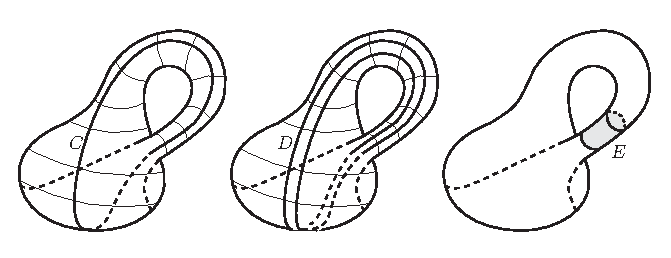
\includegraphics[width=118mm]{figures/2-10-1.pdf}\\图 2.10.1\end{center}
\item 若 $f\simeq f'$、$g\simeq g'$，证明 $f',g'$ 都有不动点。
\item 找出一个没有不动点的 Klein 瓶自映射。
\end{enumerate}
\item 设 $M$ 为 $\R^n$ 中的紧致光滑曲面，$v(x)$ 为切向量场。微分几何的标准结果说明：存在 $\epsilon>0$ 及连续映射 $F:M\times(-\epsilon,\epsilon)\to M$，使曲线 $t\mapsto F(x_0,t)$ 在 $t=0$ 经过 $x_0$，速度为 $v(x_0)$。若 $v$ 处处非零，则存在 $\delta>0$，使对所有 $x_0$ 和 $0<|t|<\delta$，都有 $F(x_0,t)\ne x_0$。
\begin{enumerate}[label=(\alph*)]
\item 利用这些事实，证明若 $M$ 有处处非零的切向量场，则 $\chi(M)=0$。
\item 确定哪些紧致曲面有处处非零的切向量场。
\end{enumerate}
\item 设多边形族 $\mathcal B$ 如定义 2.10.9。
\begin{enumerate}[label=(\alph*)]
\item 以 $|\mathcal B|$ 表示各多边形的并，证明 $\chi(\mathcal B)=\text{面数}-\text{边数}+\text{顶点数}$。［提示：从每个面的内点作星形剖分，得到单纯复形。］
\item 证明底空间同胚于 $S^2$ 的组合正则族只有五种。［提示：几何条件给出 $k\geq3$、$\ell\geq3$。］\translatornote{这里应按组合类型理解“五种”，并非指其在 $\R^3$ 中只有五种具体几何嵌入。}
\item 底空间同胚于环面的组合正则族有许多，但 $k,\ell$ 的可能值有限，求这些可能值。
\end{enumerate}
\item 设 $B\subset\R^N$ 为开单位球，举出没有不动点的连续自映射；再举出同时为一一且满的例子。
\item 设 $B^N$ 为闭单位球，举出不连续且没有不动点的自映射。
\item 令 $S=\{(\cos t,\sin t,t):0\leq t\leq4\pi\}$，$E=\{x\in\R^3:\operatorname{dist}(x,S)\leq1/10\}$，证明每个连续映射 $f:E\to E$ 都有不动点。
\end{enumerate}

\chapter{相对同调与 Eilenberg--Steenrod 公理}
\section{引言}
\sourcepage{150}
到目前为止，我们主要研究“绝对”单纯同调群，尽管已经定义相对同调群并证明其拓扑不变性。现在将更详细地研究相对群。它们有许多用途：一方面，它们在拓扑的许多应用中自然出现；另一方面，要表述同调的基本性质，即 Eilenberg--Steenrod 公理，它们是不可缺少的。

相对同调群的一种用途，是提供关于绝对同调群的信息。$H_p(K,K_0)$ 与 $H_p(K),H_p(K_0)$ 之间存在联系。例如，若 $H_p(K,K_0)$ 和 $H_{p+1}(K,K_0)$ 都为零，则 $H_p(K)$ 与 $H_p(K_0)$ 同构。这并不显然，如何精确而一般地表述这种关系，是一个微妙的问题。

代数拓扑早期，这类定理的表述往往笨拙冗长，需要恰当的语言。Eilenberg 的一个出色代数思想使问题大为澄清：它实际上只是一种方便的新记号，称为群、环或其他代数结构的“正合列”。这一概念在代数与拓扑中的作用，怎么强调都不为过。含混的代数论证用正合列表述后往往变得十分透明；另一些连专业代数学家都觉得困难的论证，也变得足够直接，可以放心地留给读者。

若本章有关群的某些术语不熟悉，请参阅第 1.5 节。

\section{同调正合列}
\sourcepage{151--152}
绝对同调与相对同调之间的关系由所谓“偶的同调正合列”表述。本节研究群的正合列，通常是阿贝尔群，并定义偶的同调正合列。

\entry{定义}{3.2.1}考虑有限或无限的群与同态序列 $\cdots\to A_1\xrightarrow{\varphi_1}A_2\xrightarrow{\varphi_2}A_3\to\cdots$。若 $\operatorname{im}\varphi_1=\ker\varphi_2$，则称在 $A_2$ 处\textbf{正合}（exact）。若在每个群处都正合，则称为\textbf{正合列}（exact sequence）。若序列有首项或末项，则不在这些端点定义正合性。

下个引理的各项应当已很熟悉，证明留作习题。因为只考虑阿贝尔群，以 $0$ 表示单元素平凡群。

\entry{引理}{3.2.2}有下列事实：
\begin{enumerate}[label=(\arabic*)]
\item $A_1\xrightarrow{\varphi}A_2\to0$ 正合，当且仅当 $\varphi$ 满射。
\item $0\to A_1\xrightarrow{\varphi}A_2$ 正合，当且仅当 $\varphi$ 单射。
\item 若 $0\to A_1\xrightarrow{\varphi}A_2\xrightarrow{\psi}A_3\to0$ 正合，称为\textbf{短正合列}（short exact sequence）。$\psi$ 诱导 $A_2/\varphi(A_1)\cong A_3$。反过来，若 $\psi:A\to B$ 满射，核为 $K$，则 $0\to K\xrightarrow{i}A\xrightarrow{\psi}B\to0$ 正合，$i$ 为包含。
\item 若 $A_1\xrightarrow{\alpha}A_2\xrightarrow{\varphi}A_3\xrightarrow{\beta}A_4$ 正合，则以下等价：(i) $\alpha$ 满射；(ii) $\beta$ 单射；(iii) $\varphi$ 为零同态。
\item 若 $A_1\xrightarrow{\alpha}A_2\to A_3\to A_4\xrightarrow{\beta}A_5$ 正合，则诱导序列 $0\to\operatorname{cok}\alpha\to A_3\to\ker\beta\to0$ 也正合。
\end{enumerate}

\entry{定义}{3.2.3}设两列群和同态 $\cdots\to A_i\to A_{i+1}\to\cdots$、$\cdots\to B_i\to B_{i+1}\to\cdots$ 的指标集相同。从前者到后者的\textbf{序列同态}是一族同态 $\alpha_i:A_i\to B_i$，使每个相应方块可交换，即沿横向同态再作用 $\alpha_{i+1}$，等于先作用 $\alpha_i$ 再沿下列横向同态。若每个 $\alpha_i$ 都是同构，称为\textbf{序列同构}。

例如，将链复形看作群与同态的序列，则序列同态恰好是链映射。

\entry{定义}{3.2.4}若短正合列 $0\to A_1\xrightarrow{\varphi}A_2\xrightarrow{\psi}A_3\to0$ 满足 $\varphi(A_1)$ 是 $A_2$ 的直和项，则称此列\textbf{分裂}（split）。

也就是说，$A_2=\varphi(A_1)\oplus B$，其中 $B$ 一般不唯一。$\varphi$ 给出 $A_1\cong\varphi(A_1)$，$\psi$ 给出 $B\cong A_3$。等价地，存在同构 $\theta:A_2\to A_1\oplus A_3$，使
\[
\begin{array}{ccccccccc}
0&\to&A_1&\xrightarrow{\varphi}&A_2&\xrightarrow{\psi}&A_3&\to&0\\
&&\Vert&&\downarrow\scriptstyle\theta&&\Vert\\
0&\to&A_1&\xrightarrow{i}&A_1\oplus A_3&\xrightarrow{\pi}&A_3&\to&0
\end{array}
\]
可交换，其中为外直和，$i$ 是包含，$\pi$ 是投影。$\theta$ 在第一直和项上取 $\varphi^{-1}$，在第二项上取 $\psi$。

\sourcepage{153--154}
\entry{定理}{3.2.5}对上述短正合列，下列条件等价：
\begin{enumerate}[label=(\arabic*)]
\item 此列分裂。
\item 存在同态 $p:A_2\to A_1$，使 $p\varphi=i_{A_1}$。
\item 存在同态 $j:A_3\to A_2$，使 $\psi j=i_{A_3}$。
\end{enumerate}
\noindent\textbf{证明：}(1) 蕴含 (2)、(3)：只需对标准列 $0\to A_1\to A_1\oplus A_3\to A_3\to0$ 验证。取 $p$ 为投影，$j$ 为包含即可。

(2) 蕴含 (1)：证明 $A_2=\varphi(A_1)\oplus\ker p$。每个 $x\in A_2$ 可写成 $x=\varphi p(x)+(x-\varphi p(x))$，前项在 $\varphi(A_1)$，后项在 $\ker p$，因为 $p(x-\varphi p(x))=p(x)-(p\varphi)p(x)=0$。若 $x\in\varphi(A_1)\cap\ker p$，写作 $x=\varphi(y)$，则 $0=p(x)=p\varphi(y)=y$，故 $x=0$。

(3) 蕴含 (1)：证明 $A_2=\ker\psi\oplus j(A_3)$，因为 $\ker\psi=\operatorname{im}\varphi$。写作 $x=(x-j\psi(x))+j\psi(x)$。前项在核中，因为 $\psi(x)-(\psi j)\psi(x)=0$；后项显然在像中。若 $x=j(z)$ 也在核中，则 $0=\psi(x)=\psi j(z)=z$，所以 $x=0$。\hfill$\square$

\entry{推论}{3.2.6}若短正合列的末端群 $A_3$ 自由阿贝尔，则此列分裂。

\noindent\textbf{证明：}选择 $A_3$ 的一组基。对每个基元素 $e$，从非空集合 $\psi^{-1}(e)$ 中选取一个元素作为 $j(e)$，再唯一扩张为同态 $j$，满足 $\psi j=i$。\hfill$\square$

现在可描述偶的同调正合列。先定义由边界算子诱导的\textbf{同调边界同态}
\[
\partial_*:H_p(K,K_0)\to H_{p-1}(K_0).
\]
给定相对闭链 $z\in C_p(K,K_0)$，它是某条 $K$ 的链 $d$ 模 $C_p(K_0)$ 的陪集，且 $\partial d$ 由 $K_0$ 承载。$\partial d$ 自动为 $K_0$ 的闭链，定义 $\partial_*\{z\}=\{\partial d\}$，花括号表示同调类。将在引理 3.3.2 证明中说明良定义性。

代数上，令 $i:K_0\to K$、$\pi:(K,\varnothing)\to(K,K_0)$ 为包含。$i_\#$ 是链群的包含，$\pi_\#$ 是商投影。给定相对闭链 $z$，先选择 $d$ 使 $\pi_\#d=z$，取边界 $\partial d$，它等于 $i_\#c$，其中 $c\in C_{p-1}(K_0)$ 为闭链。定义 $\partial_*\{z\}=\{c\}$。这一“之字形”过程即：沿 $\pi_\#$ 取原像，作用 $\partial$，再沿 $i_\#$ 取原像。下一节将用到此描述。

\entry{定义}{3.2.7}\textbf{长正合列}（long exact sequence）是以整数集为指标集的正合列，即向两端无限延伸；其中一端可以是无限串平凡群。

\entry{定理}{3.2.8（偶的同调正合列）}若 $K_0$ 为 $K$ 的子复形，则有长正合列
\[
\cdots\to H_p(K_0)\xrightarrow{i_*}H_p(K)
\xrightarrow{\pi_*}H_p(K,K_0)\xrightarrow{\partial_*}H_{p-1}(K_0)\to\cdots.
\]
其中 $i,\pi$ 为上述包含，$\partial_*$ 由边界诱导。约化同调中也有类似正合列：
\[
\cdots\to\widetilde H_p(K_0)\to\widetilde H_p(K)
\to H_p(K,K_0)\to\widetilde H_{p-1}(K_0)\to\cdots.
\]
\translatornote{约化形式使用非空 $K_0$ 的标准增广；若 $K_0$ 为空，需另行处理零维部分。}

\sourcepage{155--156}
证明基本上是代数性的。下一节将作纯代数表述并证明，见引理 3.3.2 及其后的说明。现在应用于具体例子。

\entry{例}{3.2.9}图 3.2.1 的复形 $K$ 为正方形区域，$K_0$ 为其边界。由例 1.10.4，$H_2(K,K_0)$ 为无限循环群，由所有逆时针定向 $2$ 维单形的和 $\gamma$ 生成。$H_1(K_0)$ 也为无限循环群，由 $s_1+s_2+s_3+s_4=\partial\gamma$ 生成。因此 $\partial_*:H_2(K,K_0)\to H_1(K_0)$ 为同构。
\begin{center}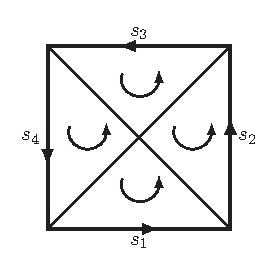
\includegraphics[width=50mm]{figures/3-2-1.pdf}\\图 3.2.1\end{center}
也可看正合列的一段 $H_2(K)\to H_2(K,K_0)\xrightarrow{\partial_*}H_1(K_0)\to H_1(K)$。因为 $|K|$ 可缩，两端群为零，故由引理 3.2.2(1)、(2)，中间映射为同构。

\entry{例}{3.2.10}图 3.2.2 中 $K$ 为环带，$K_0$ 为内外边界的并。例 1.10.5 已算过其相对同调，现在用正合列重算。
\begin{center}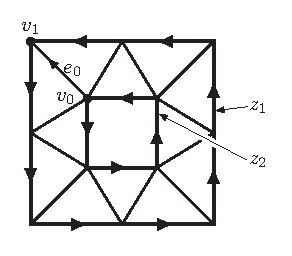
\includegraphics[width=52mm]{figures/3-2-2.pdf}\\图 3.2.2\end{center}
约化长正合列的一段为
\[
\begin{aligned}
0\to H_2(K,K_0)&\xrightarrow{\partial_*}H_1(K_0)\xrightarrow{i_*}H_1(K)\\
&\xrightarrow{\pi_*}H_1(K,K_0)\xrightarrow{\partial_*}\widetilde H_0(K_0)\to0.
\end{aligned}
\]
已知各群依次为 $0,\ ?,\ \Z\oplus\Z,\ \Z,\ ?,\ \Z,\ 0$。两端为零，因为 $|K|$ 与圆周同伦等价。$H_1(K)$ 可由绕外边界的 $z_1$ 或绕内边界的 $z_2$ 生成，两闭链同调。$K_0$ 为两个圆周的不交并，故 $H_1(K_0)$ 以 $\{z_1\},\{z_2\}$ 为基，而 $\widetilde H_0(K_0)\cong\Z$ 由 $\{v_1-v_0\}$ 生成。\translatornote{原文此处写作 $v_1-v_2$，但图中顶点为 $v_0,v_1$，后文边界也为 $v_1-v_0$。}

$i_*$ 将两基元素映到同一个生成元，所以它满射，其核由 $\{z_1\}-\{z_2\}$ 生成，为无限循环群。由满射性，$\pi_*=0$，故 $\partial_*:H_1(K,K_0)\to\widetilde H_0(K_0)$ 为同构。因此 $H_1(K,K_0)\cong\Z$，由边界为 $v_1-v_0$ 的链 $e_0$ 代表生成元。

另一方面，$\partial_*:H_2(K,K_0)\to\ker i_*$ 为同构，所以 $H_2(K,K_0)\cong\Z$。所有逆时针定向 $2$ 维单形之和 $\gamma$ 代表生成元，因为其边界在相差符号的意义下等于 $z_1-z_2$，代表核的生成元。

\sourcepage{157--158}
\entry{例}{3.2.11}同时考察两个例子：圆柱面及其上边界，或 Möbius 带及其唯一边界。两种情况下，$|K_0|$ 均为圆周，$|K|$ 也具有圆周同伦型。图 3.2.3 的中心圆周 $C$ 为形变收缩核。
\begin{center}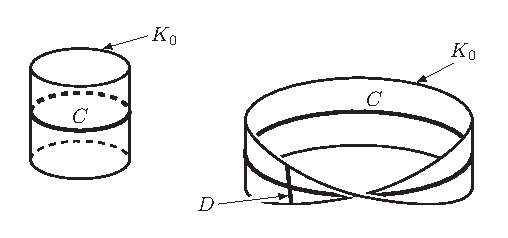
\includegraphics[width=91mm]{figures/3-2-3.pdf}\\图 3.2.3\end{center}
正合列相应片段的已知群为
\[
0\to H_2(K,K_0)\to\Z\xrightarrow{i_*}\Z\to H_1(K,K_0)\to0.
\]
关键是求 $i_*$。由于收缩 $r:|K|\to C$ 为同伦等价，只需求复合 $ri:|K_0|\to C$ 的作用。圆柱面情况下此映射的度为 $1$，而 Möbius 带情况下为乘以 $2$。所以圆柱面有 $H_2(K,K_0)=H_1(K,K_0)=0$；Möbius 带有 $H_2(K,K_0)=0$、$H_1(K,K_0)\cong\Z/2$。后一群的非零元素由中心圆周 $C$ 代表，也可由链 $D$ 代表，留作习题。

\subsection*{习题}
\begin{enumerate}
\item 验证引理 3.2.2 的 (1)--(5)。
\item \begin{enumerate}[label=(\alph*)]
\item 若 $A_i\xrightarrow{\alpha_i}B_i\xrightarrow{\beta_i}C_i$ 对 $i=1,2$ 均正合，证明乘积序列 $A_1\times A_2\xrightarrow{\alpha_1\times\alpha_2}B_1\times B_2\xrightarrow{\beta_1\times\beta_2}C_1\times C_2$ 正合。
\item 推广到任意直积。
\item 推广到任意直和。
\end{enumerate}
\item 若 $K_0$ 无环，证明 $H_i(K,K_0)\cong\widetilde H_i(K)$。
\item 若包含 $|K_0|\to|K|$ 为同伦等价，证明所有 $H_p(K,K_0)$ 为零。
\item 对例 3.2.11 的 Möbius 带偶，证明其非零相对一维同调类由图中的 $D$ 代表。
\item 设 $S$ 为 Klein 瓶，$A,C$ 为通常的简单闭曲线，见第 2.6 节习题 2。计算偶 $(S,A)$ 与 $(S,C)$ 的正合列。
\item 对正合列 $A\xrightarrow{\alpha}B\xrightarrow{\beta}C\xrightarrow{\gamma}D$，证明 $D\ne0$ 时 $\beta$ 不一定满射。
\item 对同一正合列，证明 $A\ne0$ 时 $\beta$ 不一定单射。
\end{enumerate}

\section{之字形引理}
\sourcepage{158--159}
本节证明偶的同调序列正合。我们将其重新表述为链复形的定理，再在这个形式下证明。先作一个定义。

\entry{定义}{3.3.1}设 $\mathcal C,\mathcal D,\mathcal E$ 为链复形，以 $0$ 表示各维群均为零的平凡链复形。若链映射组成的序列
\[
0\to\mathcal C\xrightarrow{\varphi}\mathcal D\xrightarrow{\psi}\mathcal E\to0
\]
在每个维数 $p$ 上都给出群的短正合列 $0\to C_p\xrightarrow{\varphi}D_p\xrightarrow{\psi}E_p\to0$，则称其为\textbf{链复形的短正合列}。

例如，$0\to\mathcal C(K_0)\to\mathcal C(K)\to\mathcal C(K,K_0)\to0$ 正合，因为相对链群按定义就是商群。

\entry{引理}{3.3.2（之字形引理）}设链复形 $\mathcal C=\{C_p,\partial_C\}$、$\mathcal D=\{D_p,\partial_D\}$、$\mathcal E=\{E_p,\partial_E\}$ 组成上述短正合列，则有长正合列
\[
\cdots\to H_p(\mathcal C)\xrightarrow{\varphi_*}H_p(\mathcal D)
\xrightarrow{\psi_*}H_p(\mathcal E)\xrightarrow{\partial_*}H_{p-1}(\mathcal C)
\xrightarrow{\varphi_*}H_{p-1}(\mathcal D)\to\cdots,
\]
其中 $\partial_*$ 由 $\mathcal D$ 的边界算子诱导。

\noindent\textbf{证明：}这种证明通常称为“图表追踪”（diagram chasing）。以后大多数此类证明将留给读者。所用交换图由各维短正合列及竖直边界算子组成：
\[
\begin{array}{ccccccccc}
0&\to&C_{p+1}&\xrightarrow{\varphi}&D_{p+1}&\xrightarrow{\psi}&E_{p+1}&\to&0\\
&&\downarrow\scriptstyle\partial_C&&\downarrow\scriptstyle\partial_D&&\downarrow\scriptstyle\partial_E\\
0&\to&C_p&\xrightarrow{\varphi}&D_p&\xrightarrow{\psi}&E_p&\to&0\\
&&\downarrow\scriptstyle\partial_C&&\downarrow\scriptstyle\partial_D&&\downarrow\scriptstyle\partial_E\\
0&\to&C_{p-1}&\xrightarrow{\varphi}&D_{p-1}&\xrightarrow{\psi}&E_{p-1}&\to&0.
\end{array}
\]
\textbf{第一步。}定义 $\partial_*$。给定闭链 $e_p\in E_p$，由满射性选 $d_p\in D_p$ 使 $\psi(d_p)=e_p$。因为
\[
\psi(\partial_Dd_p)=\partial_E\psi(d_p)=\partial_Ee_p=0,
\]
所以 $\partial_Dd_p\in\ker\psi=\operatorname{im}\varphi$。存在唯一 $c_{p-1}$，使 $\varphi(c_{p-1})=\partial_Dd_p$。又有
\[
\varphi(\partial_Cc_{p-1})=\partial_D\varphi(c_{p-1})=\partial_D^2d_p=0.
\]
由 $\varphi$ 单射，$c_{p-1}$ 为闭链。定义 $\partial_*\{e_p\}=\{c_{p-1}\}$。

\sourcepage{160}
\textbf{第二步。}验证其为良定义同态。设闭链 $e_p,e'_p$ 分别提升为 $d_p,d'_p$，并相应得到 $c_{p-1},c'_{p-1}$。若 $e_p-e'_p=\partial_Ee_{p+1}$，选择 $d_{p+1}$ 使 $\psi(d_{p+1})=e_{p+1}$，则
\[
\psi(d_p-d'_p-\partial_Dd_{p+1})
=e_p-e'_p-\partial_Ee_{p+1}=0.
\]
所以存在 $c_p$，使 $\varphi(c_p)=d_p-d'_p-\partial_Dd_{p+1}$。取边界得
\[
\varphi(\partial_Cc_p)=\partial_D(d_p-d'_p)
=\varphi(c_{p-1}-c'_{p-1}).
\]
由单射性，$\partial_Cc_p=c_{p-1}-c'_{p-1}$，故同调类相同。又因为 $d_p+d'_p$ 可提升 $e_p+e'_p$，相应链为 $c_{p-1}+c'_{p-1}$，所以 $\partial_*$ 保持加法。

\textbf{第三步。}证明在 $H_p(\mathcal D)$ 处正合。由 $\psi\varphi=0$，有 $\operatorname{im}\varphi_*\subset\ker\psi_*$。反过来，若 $\psi_*\{d_p\}=0$，则 $\psi(d_p)=\partial_Ee_{p+1}$。提升 $e_{p+1}$ 为 $d_{p+1}$，得到
\[
\psi(d_p-\partial_Dd_{p+1})=0,
\]
故 $d_p-\partial_Dd_{p+1}=\varphi(c_p)$。因 $d_p$ 为闭链，$\varphi(\partial_Cc_p)=0$，所以 $c_p$ 为闭链。而
\[
\varphi_*\{c_p\}=\{d_p-\partial_Dd_{p+1}\}=\{d_p\},
\]
得到反向包含。

\sourcepage{161}
\textbf{第四步。}证明在 $H_p(\mathcal E)$ 处正合。给定 $\alpha=\{e_p\}$，选取 $d_p,c_{p-1}$ 如第一步。若 $\alpha$ 属于 $\operatorname{im}\psi_*$，可选择 $d_p$ 为闭链，则 $\varphi(c_{p-1})=0$，故 $c_{p-1}=0$，$\partial_*\alpha=0$。

反过来，若 $\partial_*\alpha=0$，则 $c_{p-1}=\partial_Cc_p$。链 $d_p-\varphi(c_p)$ 为闭链，因为
\[
\partial_D(d_p-\varphi(c_p))=\partial_Dd_p-\varphi(c_{p-1})=0.
\]
且 $\psi_*\{d_p-\varphi(c_p)\}=\{e_p\}=\alpha$，故 $\alpha\in\operatorname{im}\psi_*$。

\textbf{第五步。}证明在 $H_{p-1}(\mathcal C)$ 处正合。若 $\beta\in\operatorname{im}\partial_*$，则可写成 $\beta=\{c_{p-1}\}$，且 $\varphi(c_{p-1})=\partial_Dd_p$，所以 $\varphi_*\beta=0$。反过来，若 $\varphi_*\{c_{p-1}\}=0$，则存在 $d_p$ 使 $\varphi(c_{p-1})=\partial_Dd_p$。令 $e_p=\psi(d_p)$，则
\[
\partial_Ee_p=\psi\partial_Dd_p=\psi\varphi(c_{p-1})=0,
\]
且按定义 $\partial_*\{e_p\}=\{c_{p-1}\}$，得到所需结论。\hfill$\square$

整个证明没有假设链复形自由或非负，故其适用范围远超单纯链群。应用于 $\mathcal C(K_0),\mathcal C(K),\mathcal C(K,K_0)$，立即得到普通同调的定理 3.2.8。

对约化同调，仍取 $\mathcal E=\mathcal C(K,K_0)$，将前两个复形增广。由于包含保持增广，在 $-1$ 维短正合列为 $0\to\Z\xrightarrow{i}\Z\to0\to0$，且与零维边界可交换。再用之字形引理，即得约化版本。

从证明中还能提取自然性：给每个链复形短正合列指定同调长正合列，这一操作将短正合列同态变为相应长正合列同态。

\sourcepage{162}
\entry{定理}{3.3.3}设下图可交换，各横列为链复形短正合列，竖向为链映射：
\[
\begin{array}{ccccccccc}
0&\to&\mathcal C&\xrightarrow{\varphi}&\mathcal D&\xrightarrow{\psi}&\mathcal E&\to&0\\
&&\downarrow\scriptstyle\alpha&&\downarrow\scriptstyle\beta&&\downarrow\scriptstyle\gamma\\
0&\to&\mathcal C'&\xrightarrow{\varphi'}&\mathcal D'&\xrightarrow{\psi'}&\mathcal E'&\to&0.
\end{array}
\]
则相应同调长正合列之间由 $\alpha_*,\beta_*,\gamma_*$ 给出的图也可交换，特别地 $\partial'_*\gamma_*=\alpha_*\partial_*$。

\noindent\textbf{证明：}涉及 $\varphi_*,\psi_*$ 的方块已在链层次可交换。对于连接同态，给定 $\{e_p\}$，选 $d_p$ 使 $\psi(d_p)=e_p$，选 $c_{p-1}$ 使 $\varphi(c_{p-1})=\partial_Dd_p$。于是 $\partial_*\{e_p\}=\{c_{p-1}\}$。令 $e'_p=\gamma(e_p)$。$\beta(d_p)$ 是它的一个提升，因为 $\psi'\beta(d_p)=\gamma\psi(d_p)=e'_p$。又
\[
\varphi'\alpha(c_{p-1})=\beta\varphi(c_{p-1})
=\beta\partial_Dd_p=\partial'_D\beta(d_p).
\]
所以 $\partial'_*\{e'_p\}=\{\alpha(c_{p-1})\}=\alpha_*\partial_*\{e_p\}$。\hfill$\square$

长正合列的自然性非常有用。下面给一个应用，需要下列引理，其图表追踪证明留给读者。

\entry{引理}{3.3.4（Steenrod 五引理）}设阿贝尔群的交换图两行均正合：
\[
\begin{array}{ccccccccc}
A_1&\to&A_2&\to&A_3&\to&A_4&\to&A_5\\
\downarrow\scriptstyle f_1&&\downarrow\scriptstyle f_2&&\downarrow\scriptstyle f_3&&\downarrow\scriptstyle f_4&&\downarrow\scriptstyle f_5\\
B_1&\to&B_2&\to&B_3&\to&B_4&\to&B_5.
\end{array}
\]
若 $f_1,f_2,f_4,f_5$ 为同构，则 $f_3$ 也为同构。

\sourcepage{163--164}
\entry{引理}{3.3.5}设 $h:(K,K_0)\to(L,L_0)$ 为单纯映射。
\begin{enumerate}[label=(\alph*)]
\item 各诱导同态 $h_*$ 给出两个偶的同调正合列之间的序列同态。
\item 若 $h_*:H_i(K)\to H_i(L)$ 与 $h_*:H_i(K_0)\to H_i(L_0)$ 在 $i=p,p-1$ 时均为同构，则 $h_*:H_p(K,K_0)\to H_p(L,L_0)$ 为同构。
\item 将所有绝对同调换为约化同调，以上仍成立。
\end{enumerate}
\noindent\textbf{证明：}$h_\#$ 是链映射，且与包含、商投影可交换，所以给出链复形短正合列之间的同态，由定理得 (a)。对约化情形，$h_\#$ 保持增广，在 $-1$ 维定义为 $\Z$ 的恒等映射，即可应用增广后的结论。(b) 直接由五引理得到。\hfill$\square$

\entry{定理}{3.3.6}前一引理对任意连续映射 $h:(|K|,|K_0|)\to(|L|,|L_0|)$ 也成立。

这是前一引理与第二章结果的直接推论。偶的长正合列之外，还有三元组的长正合列，存在性留作习题 1。

\entry{定义}{3.3.7}若 $X$ 为复形，$A$ 为其子复形，$B$ 为 $A$ 的子复形，则称 $(X,A,B)$ 为\textbf{单纯三元组}（simplicial triple），语境明确时简称三元组。

\entry{定理}{3.3.8（三元组的同调正合列）}对于单纯三元组 $(X,A,B)$，存在自然的长正合列
\[
\cdots\to H_i(A,B)\to H_i(X,B)\to H_i(X,A)\to H_{i-1}(A,B)\to\cdots.
\]
下面的结果留作习题 2。

\entry{引理}{3.3.9（蛇引理）}给定阿贝尔群短正合列之间的同态
\[
\begin{array}{ccccccccc}
0&\to&A&\to&B&\to&C&\to&0\\
&&\downarrow\scriptstyle\alpha&&\downarrow\scriptstyle\beta&&\downarrow\scriptstyle\gamma\\
0&\to&D&\to&E&\to&F&\to&0,
\end{array}
\]
则有正合列
\[
0\to\ker\alpha\to\ker\beta\to\ker\gamma\to
\operatorname{cok}\alpha\to\operatorname{cok}\beta\to\operatorname{cok}\gamma\to0.
\]
原书以 serpent lemma 称呼它，脚注指出也称 snake lemma。

习题 7 涉及 Bockstein 同态，定义如下。

\entry{定义}{3.3.10}给定复形 $K$ 及阿贝尔群短正合列 $0\to G\to G'\to G''\to0$，得到系数链复形的短正合列
\[
0\to C_p(K;G)\to C_p(K;G')\to C_p(K;G'')\to0.
\]
它给出同调长正合列，其中的之字形同态通常记为
\[
\beta_*:H_p(K;G'')\to H_{p-1}(K;G),
\]
称为相应系数序列的 \textbf{Bockstein 同态}。

\sourcepage{164--165}
\subsection*{习题}
\begin{enumerate}
\item 证明三元组同调正合列的存在性与自然性。
\item 证明蛇引理。［提示：应用之字形引理。］
\item \begin{enumerate}[label=(\alph*)]
\item 证明 Steenrod 五引理。
\item 对五引理的交换图，考虑八个假设：$i=1,2,4,5$ 时 $f_i$ 分别为单射，以及分别为满射。哪些假设足以推出 $f_3$ 单射？哪些足以推出其满射？
\end{enumerate}
\item 举例说明，即使所有 $i$ 都有 $H_i(K_0)\cong H_i(L_0)$、$H_i(K)\cong H_i(L)$，相对同调也不一定同构。
\item 对锥 $w*K$，证明 $H_i(w*K,K)\cong\widetilde H_{i-1}(K)$。
\item 设 $K_0$ 为 $K$ 的子复形。
\begin{enumerate}[label=(\alph*)]
\item 若存在收缩映射 $r:|K|\to|K_0|$，证明 $H_p(K)\cong H_p(K,K_0)\oplus H_p(K_0)$。
\item 若 $|K|$ 的恒等映射同伦于将 $|K|$ 映入 $|K_0|$ 的映射，证明 $H_p(K_0)\cong H_p(K)\oplus H_{p+1}(K,K_0)$。
\item 若包含 $j:|K_0|\to|K|$ 同伦于常值映射，证明
\[
H_p(K,K_0)\cong\widetilde H_p(K)\oplus\widetilde H_{p-1}(K_0).
\]
［提示：证明 $j$ 扩张为 $f:|w*K_0|\to|K|$，见推论 2.8.8，再应用习题 5。］
\item[\textasteriskcentered\,(d)] 举例说明：若只假设 $j_*$ 在约化同调中为零，(c) 的结论未必成立。
\end{enumerate}
\item \begin{enumerate}[label=(\alph*)]
\item 当 $|K|=P^2$ 时，分别计算系数序列 $0\to\Z\to\Z\to\Z/2\to0$ 和 $0\to\Z/2\to\Z/4\to\Z/2\to0$ 的 Bockstein 同态。
\item 当 $|K|$ 为 Klein 瓶时，重复 (a)。
\end{enumerate}
\item 证明定理 3.3.6。
\end{enumerate}

\section{Mayer--Vietoris 序列}
\sourcepage{165--166}
同调正合列是计算同调群的有用工具，另一个工具是下面构造的 Mayer--Vietoris 序列。它也是之字形引理的推论。

\entry{定理}{3.4.1}设 $K=K_0\cup K_1$，其中 $K_0,K_1$ 为子复形，令 $A=K_0\cap K_1$。则存在正合列
\[
\cdots\to H_p(A)\to H_p(K_0)\oplus H_p(K_1)\to H_p(K)\to H_{p-1}(A)\to\cdots.
\]
若 $A$ 非空，约化同调中也有类似正合列。

\entry{定义}{3.4.2}此序列称为 $(K_0,K_1)$ 的 \textbf{Mayer--Vietoris 序列}。

\noindent\textbf{证明：}构造链复形短正合列
\[
0\to\mathcal C(A)\xrightarrow{\varphi}\mathcal C(K_0)\oplus\mathcal C(K_1)
\xrightarrow{\psi}\mathcal C(K)\to0,
\]
再应用之字形引理。中间复形的 $p$ 维群为 $C_p(K_0)\oplus C_p(K_1)$，边界为 $\partial'(d,e)=(\partial_0d,\partial_1e)$。

以 $i:A\to K_0$、$j:A\to K_1$、$k:K_0\to K$、$\ell:K_1\to K$ 表示包含，$m:A\to K$ 表示共同复合。定义
\[
\varphi(c)=(i_\#c,-j_\#c),\qquad
\psi(d,e)=k_\#d+\ell_\#e.
\]
它们显然为链映射。$\varphi$ 单射，因为 $i_\#$ 为包含。$\psi$ 满射：将链 $d$ 写成定向单形之和，取由 $K_0$ 承载的全部项为 $d_0$，则 $d-d_0$ 由 $K_1$ 承载，且 $\psi(d_0,d-d_0)=d$。

\sourcepage{167}
在中间项，先有 $\psi\varphi(c)=m_\#c-m_\#c=0$。反过来，若 $\psi(d,e)=0$，把两者看作 $K$ 的链，则 $d=-e$。由于分别由 $K_0,K_1$ 承载，两者均由 $A$ 承载，故 $(d,e)=(d,-d)=\varphi(d)$，证明正合。

中间复形的同调为
\[
\frac{\ker\partial'}{\operatorname{im}\partial'}
=\frac{\ker\partial_0\oplus\ker\partial_1}{\operatorname{im}\partial_0\oplus\operatorname{im}\partial_1}
\cong H_p(K_0)\oplus H_p(K_1).
\]
由之字形引理即得普通版本。

约化版本需要进一步处理。将各复形换为增广复形，零维增广映射分别为 $\epsilon_A$、$\epsilon_0\oplus\epsilon_1$ 和 $\epsilon$。在 $-1$ 维定义
\[
0\to\Z\xrightarrow{\varphi}\Z\oplus\Z\xrightarrow{\psi}\Z\to0,
\qquad\varphi(n)=(n,-n),\quad\psi(m,n)=m+n.
\]
此列正合，并与增广映射可交换。因为 $A$ 非空，各增广都满射，所以这些复形的 $-1$ 维同调为零，零维同调分别为 $\widetilde H_0(A)$、$\widetilde H_0(K_0)\oplus\widetilde H_0(K_1)$ 和 $\widetilde H_0(K)$。再用之字形引理完成证明。\hfill$\square$

\entry{引理}{3.4.3}若 $h:(K,K_0,K_1)\to(L,L_0,L_1)$ 为单纯映射，且 $K=K_0\cup K_1$、$L=L_0\cup L_1$，则 $h$ 诱导相应 Mayer--Vietoris 序列之间的同态。

\noindent\textbf{证明：}$h_\#$ 与前面定义的 $\varphi,\psi$ 可交换，自然性由定理 3.3.3 得到。\hfill$\square$

\entry{定理}{3.4.4}前一引理也适用于任意连续映射 $h:(|K|,|K_0|,|K_1|)\to(|L|,|L_0|,|L_1|)$。

这是前一引理与第二章结果的直接推论。

\sourcepage{168--169}
为说明序列的实际用途，计算复形悬挂的同调。悬挂已在定义 1.9.8 出现，为方便重述。

\entry{定义}{3.4.5}若两个锥 $w_0*K,w_1*K$ 的多胞体仅在 $|K|$ 相交，则 $S(K)=(w_0*K)\cup(w_1*K)$ 为复形，称为 $K$ 的\textbf{悬挂}。给定 $K$，悬挂在相差单纯同构的意义下唯一确定。

\entry{定理}{3.4.6}对所有 $p$，有同构 $\widetilde H_p(S(K))\to\widetilde H_{p-1}(K)$。

\noindent\textbf{证明：}令 $K_0=w_0*K$、$K_1=w_1*K$。两者的并为悬挂，交为 $K$。约化 Mayer--Vietoris 序列的片段为
\[
\begin{aligned}
\widetilde H_p(K_0)\oplus\widetilde H_p(K_1)&\to\widetilde H_p(S(K))\\
&\to\widetilde H_{p-1}(K)\to\widetilde H_{p-1}(K_0)\oplus\widetilde H_{p-1}(K_1).
\end{aligned}
\]
两端为零，因为都是锥，故中间映射为同构。\hfill$\square$

\entry{定理}{3.4.7}设 $K_0,K_1$ 为 $K$ 的子复形，$L_0,L_1$ 分别为它们的子复形，则存在正合列
\[
\begin{aligned}
\cdots\to H_i(K_0\cap K_1,L_0\cap L_1)
&\to H_i(K_0,L_0)\oplus H_i(K_1,L_1)\\
&\to H_i(K_0\cup K_1,L_0\cup L_1)\\
&\to H_{i-1}(K_0\cap K_1,L_0\cap L_1)\to\cdots.
\end{aligned}
\]
\entry{定义}{3.4.8}此序列称为\textbf{相对 Mayer--Vietoris 序列}。

\subsection*{习题}
\begin{enumerate}
\item 设 $K=K_0\cup K_1$，$|K_0|,|K_1|$ 连通。下列各情形中，能对 $K$ 的同调说些什么？
\begin{enumerate}[label=(\alph*)]
\item $K_0\cap K_1$ 非空且无环。
\item $|K_0|\cap|K_1|$ 恰有两点。
\item $K_0\cap K_1$ 具有 $S^n$ 的同调，其中 $n>0$。
\item $K_0,K_1$ 均无环。
\end{enumerate}
\item 证明定理 3.4.7 的相对序列存在。
\item 给定整数 $d$、$n\geq1$，证明存在度为 $d$ 的映射 $h:S^n\to S^n$。［提示：用序列的自然性归纳；$n=1$ 见第 2.9 节习题 1。］
\item 对第 1.9 节习题 1 的同态 $\varphi:C_p(K)\to C_{p+1}(S(K))$，证明定理 3.4.6 的同构为 $\varphi_*$ 的逆。
\item 给定有限生成阿贝尔群列 $G_0,\ldots,G_n$，其中 $G_0,G_n$ 自由，且 $G_0\ne0$，证明存在 $n$ 维有限复形 $K$，使 $H_i(K)\cong G_i$（$i=0,\ldots,n$）。［提示：第 1.7 节习题 8。］
\item 第七章将研究乘积的同调。现在假设涉及的空间均为多面体，证明：
\begin{enumerate}[label=(\alph*)]
\item 若 $p\in S^n$，则 $H_q(X\times S^n,X\times\{p\})\cong H_{q-n}(X)$。［提示：把球面写成上下半球面的并，对 $n$ 归纳。］
\item 若 $p\in Y$，偶 $(X\times Y,X\times\{p\})$ 的同调正合列分解为分裂短正合列。
\item $H_q(X\times S^n)\cong H_{q-n}(X)\oplus H_q(X)$。
\item 计算 $S^n\times S^m$ 的同调。
\end{enumerate}
\item 将习题 3 的 $S^n$ 换为 $n$ 维环面 $T^n=\underbrace{S^1\times\cdots\times S^1}_{n\text{ 个因子}}$。
\end{enumerate}

\section{Eilenberg--Steenrod 公理}
\sourcepage{169--170}
我们为特定空间类，即多面体，定义了同调群。历史上它们最先出现，后来各种推广定义适用于更一般的空间。这些同调理论有许多共同特点，在多面体上都给出与单纯同调相同的结果。

同调理论的多样性促使 Eilenberg 和 Steenrod 将其公理化。他们提炼出共同的关键性质，并证明这些性质在多面体类上完全刻画同调群。

这里不复述完整公理化方法，也不证明刻画定理，可参阅 [ES52]。我们只列出七条公理，另加处理非紧致空间所需的一条公理。下一节验证单纯同调满足它们。

\entry{定义}{3.5.1}设 $\mathcal A$ 为拓扑空间偶 $(X,A)$（$A\subset X$）的一个类，满足：
\begin{enumerate}[label=(\arabic*)]
\item 若 $(X,A)\in\mathcal A$，则 $(X,X),(X,\varnothing),(A,A),(A,\varnothing)$ 也属于此类。
\item 若 $(X,A)\in\mathcal A$，则 $(X\times I,A\times I)$ 也属于此类。
\item 存在单点空间 $P$，使 $(P,\varnothing)\in\mathcal A$。
\end{enumerate}
称 $\mathcal A$ 为同调理论的一个\textbf{容许空间类}（admissible class）。

\entry{定义}{3.5.2}若 $\mathcal A$ 容许，则其上的一个\textbf{同调理论}由三个函数组成：
\begin{enumerate}[label=(\arabic*)]
\item 对每个整数 $p$ 和偶 $(X,A)$ 指定阿贝尔群 $H_p(X,A)$。
\item 对每个连续映射 $h:(X,A)\to(Y,B)$ 指定同态 $(h_*)_p:H_p(X,A)\to H_p(Y,B)$。
\item 对每个偶指定同态 $(\partial_*)_p:H_p(X,A)\to H_{p-1}(A)$，其中 $A$ 表示 $(A,\varnothing)$。
\end{enumerate}
它们须满足下列公理，涉及的偶均在 $\mathcal A$ 中。仍省略诱导映射的维数下标。

\entry{公理}{1}恒等映射诱导恒等同态。

\entry{公理}{2}$(k\circ h)_*=k_*\circ h_*$。

\sourcepage{171}
\entry{公理}{3}若 $f:(X,A)\to(Y,B)$，则边界的自然性成立：
\[
\begin{array}{ccc}
H_p(X,A)&\xrightarrow{f_*}&H_p(Y,B)\\
\downarrow\scriptstyle\partial_*&&\downarrow\scriptstyle\partial_*\\
H_{p-1}(A)&\xrightarrow{(f|_A)_*}&H_{p-1}(B).
\end{array}
\]

\entry{公理}{4（正合公理）}序列
\[
\cdots\to H_p(A)\xrightarrow{i_*}H_p(X)\xrightarrow{\pi_*}H_p(X,A)
\xrightarrow{\partial_*}H_{p-1}(A)\to\cdots
\]
正合，其中 $i:A\to X$、$\pi:X\to(X,A)$ 为包含。

回顾：$h,k:(X,A)\to(Y,B)$ 同伦，指存在连续 $F:(X\times I,A\times I)\to(Y,B)$，满足 $F(x,0)=h(x)$、$F(x,1)=k(x)$。

\entry{公理}{5（同伦公理）}若 $h\simeq k$，则 $h_*=k_*$。

\entry{公理}{6（切除公理）}给定 $(X,A)$，若 $U$ 在 $X$ 中开，$\overline U\subset\Int A$，且 $(X\setminus U,A\setminus U)$ 容许，则包含诱导同构
\[
H_p(X\setminus U,A\setminus U)\cong H_p(X,A).
\]

\entry{公理}{7（维数公理）}若 $P$ 为单点空间，则 $p\ne0$ 时 $H_p(P)=0$，而 $H_0(P)=\Z$。

\entry{公理}{8（紧支撑公理）}若 $\alpha\in H_p(X,A)$，则存在容许偶 $(X_0,A_0)$，其中 $X_0,A_0$ 紧致，使 $\alpha$ 属于包含诱导同态 $H_p(X_0,A_0)\to H_p(X,A)$ 的像。

两空间均紧致的偶称为\textbf{紧致偶}。也可把维数公理改为 $H_0(P)=G$，其中 $G$ 为固定阿贝尔群，得到“以 $G$ 为系数的同调”。目前仍使用整数系数。

维数公理似乎最无害、最不有趣，但在某种意义上恰好相反。公理提出后，人们发现了类似同调的新理论，例如微分拓扑的配边理论和向量丛理论中的 K 理论。它们的发明目的与同调群最初的目的很不同，却共享许多形式性质，尤其满足除维数公理外的 Eilenberg--Steenrod 公理。

\sourcepage{172}
如今称这种理论为\textbf{非普通同调理论}（extraordinary homology theory），或\textbf{广义同调理论}（generalized homology theory）。它与普通同调的区别是，单点空间也可能在许多维数上有非零同调。这说明数学中反复出现的现象：为一种目的建立的理论，会产生远超创始者预想的后果。

以下定义用于习题 1。

\entry{定义}{3.5.3}下列阿贝尔群及同态的交换图称为\textbf{辫形图}（braid）：
\begin{center}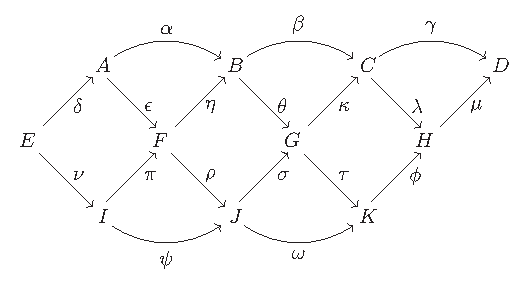
\includegraphics[width=114mm]{figures/3-5-braid.pdf}\end{center}
图中有四列，形如相互叠合的正弦曲线。前三列为
\[
\left.\begin{aligned}
E&\to A\to B\to G\to K,\\
E&\to I\to J\to G\to C\to D,\\
A&\to F\to J\to K\to H\to D,
\end{aligned}\right\}\tag{$*$}
\]
第四列为 $I\to F\to B\to C\to H$。若四列均正合，称为\textbf{正合辫形图}。

\entry{引理}{3.5.4（辫形图引理）}若 $(*)$ 的三列正合，且复合 $I\to F\to B$ 为零，则整个辫形图正合。

以下定义用于习题 3。

\entry{定义}{3.5.5}设 $X=X_1\cup X_2$，$A=X_1\cap X_2$。若 $(X_1,A)$、$(X,X_2)$ 容许，且包含 $(X_1,A)\to(X,X_2)$ 诱导同调同构，则称 $(X_1,X_2)$ 为给定同调理论的\textbf{可切除空间对}（excisive couple）。

\sourcepage{173--174}
\subsection*{习题}
\begin{enumerate}
\item \begin{enumerate}[label=(\alph*)]
\item 若定义 3.5.3 的辫形图正合，证明存在同构 $\Lambda:(\ker\omega)/(\operatorname{im}\psi)\to(\ker\beta)/(\operatorname{im}\alpha)$，定义如下：若 $\omega(j)=0$，选 $f$ 使 $\rho(f)=j$，令 $\Lambda(\{j\})=\{\eta(f)\}$。
\item 证明辫形图引理。
\end{enumerate}
\item 设 $X\supset A\supset B$，称 $(X,A,B)$ 为拓扑空间三元组，同调语境下默认上述嵌套关系。仅使用同调公理，证明三元组同调序列
\[
\cdots\to H_p(A,B)\xrightarrow{\pi}H_p(X,B)\xrightarrow{\eta}H_p(X,A)
\xrightarrow{\beta}H_{p-1}(A,B)\to\cdots
\]
正合，其中 $\pi,\eta$ 由包含诱导，$\beta$ 为复合 $H_p(X,A)\xrightarrow{\partial_*}H_{p-1}(A)\xrightarrow{i_*}H_{p-1}(A,B)$。假定各偶容许。［提示：证明 $H_p(A,A)=0$、$\eta\pi=0$，再用习题 1。］
\item 仅使用公理，按下列方法导出 Mayer--Vietoris 序列。
\begin{enumerate}[label=(\alph*)]
\item 设 $i:A\to X_1$、$j:A\to X_2$、$k:X_1\to X$、$\ell:X_2\to X$ 为包含，$\alpha:X_1\to(X_1,A)$、$\beta:X\to(X,X_2)$ 及 $\gamma:(X_1,A)\to(X,X_2)$ 也为包含，给出相应的长正合列同态。若 $(X_1,X_2)$ 可切除，按
\[
\begin{aligned}
\varphi(a)&=(i_*a,-j_*a),\\
\psi(x_1,x_2)&=k_*x_1+\ell_*x_2,\\
\theta(x)&=\partial_*\gamma_*^{-1}\beta_*(x)
\end{aligned}
\]
定义序列 $\cdots\to H_p(A)\xrightarrow{\varphi}H_p(X_1)\oplus H_p(X_2)\xrightarrow{\psi}H_p(X)\xrightarrow{\theta}H_{p-1}(A)\to\cdots$。其中 $\partial_*$ 为 $(X_1,A)$ 的边界同态。证明它正合，且对于连续映射诱导的同态自然。［提示：作图表追踪，从每隔三个位置就是同构的长正合列同态出发。］
\item 若 $X=|K|$，$X_1,X_2$ 为子复形的多胞体，证明它们对单纯同调可切除，且所得序列就是定理 3.4.1 的序列。
\item 假定 $(X_1,A)$、$(X,X_2)$ 容许。若 $\Int X_1$ 与 $\Int X_2$ 覆盖 $X$，且 $X_1$ 在 $X$ 中闭，证明此空间对对任何满足公理的同调理论都可切除。
\end{enumerate}
\end{enumerate}

\section{单纯理论的公理}
\sourcepage{174--175}
验证公理之前，必须更仔细地处理几个问题。公理要求在容许空间类上定义同调群。严格地说，我们只对单纯复形定义了群，并未对空间定义。一个多面体可以由许多不同复形实现，它们的同调群自然同构，却仍是不同的群。同样，连续映射 $h:X\to Y$ 在选择 $X=|K|,Y=|L|$ 后诱导 $H_p(K)\to H_p(L)$，换成其他复形又得到另一同态，却都记为 $h_*$。此前已经指出这种记号歧义。

解决方法是再作一层抽象：将所有底空间为 $X$ 的复形的同调群自然地等同，所得群称为空间的同调群。更一般地，可对任何同胚于多面体的空间这样做，细节如下。

\entry{定义}{3.6.1}空间偶 $(X,A)$ 的一个\textbf{三角剖分}是复形 $K$、子复形 $K_0$ 及同胚 $h:(|K|,|K_0|)\to(X,A)$。若存在，称其为\textbf{可三角剖分偶}。$A$ 为空时，与定义 2.9.7 一致，只称 $X$ 可三角剖分。

设 $(X,A)$ 可三角剖分，考虑其全部三角剖分 $h_\alpha:(|K_\alpha|,|C_\alpha|)\to(X,A)$。这里存在类似“所有集合的集合”的集合论问题。为避免它，要求各 $K_\alpha$ 位于固定空间 $E^J$。只要 $J$ 足够大，每个复形都有同构副本位于其中；例如可取 $J$ 的基数等于 $X$ 的基数。限定在固定空间之后，就能用足够大的指标集编号。

固定 $p$，用 $H_p(K_\alpha,C_\alpha)\times\{\alpha\}$ 使各群作为集合不交。在不交并
\[
\coprod_\alpha H_p(K_\alpha,C_\alpha)\times\{\alpha\}\tag{$*$}
\]
上定义等价关系：$(x,\alpha)$ 与 $(y,\beta)$ 等价，当且仅当 $(h_\beta^{-1}h_\alpha)_*(x)=y$。定义 $H_p(X,A)$ 为这些等价类的集合。

每个等价类在每个带标签群中恰有一个元素，所以将元素映到其等价类的映射为双射。要求它成为群同构，以此给 $H_p(X,A)$ 群结构。因为各过渡映射 $(h_\beta^{-1}h_\alpha)_*$ 都为同构，此结构无歧义。

\sourcepage{176}
连续映射 $h:(X,A)\to(Y,B)$ 也诱导同态。任选两偶的剖分 $h_\alpha:(|K_\alpha|,|C_\alpha|)\to(X,A)$ 和 $k_\beta:(|L_\beta|,|D_\beta|)\to(Y,B)$，形成 $h'=k_\beta^{-1}hh_\alpha$。其诱导同态 $h'_*:H_p(K_\alpha,C_\alpha)\to H_p(L_\beta,D_\beta)$ 通过等价类给出良定义的 $h_*:H_p(X,A)\to H_p(Y,B)$。

同样，复形上的边界同态诱导 $\partial_*:H_p(X,A)\to H_{p-1}(A)$。同调理论所需的各部分已经齐备。

可三角剖分偶构成容许类：所要求的 $(X,X),(X,\varnothing),(A,A),(A,\varnothing)$ 显然可剖分，单点空间可剖分，乘积偶则由引理 2.7.3 得到。

\entry{定理}{3.6.2}可三角剖分偶上的单纯同调满足 Eilenberg--Steenrod 公理。

\noindent\textbf{证明：}公理 1--5、7 是已熟悉的复形同调性质，立即推广到空间偶。只需进一步思考紧支撑和切除公理。

先证紧支撑。设 $\alpha\in H_p(K,K_0)$，取代表链 $c$，其边界由 $K_0$ 承载。$c$ 由某个有限子复形 $L$ 承载，因此可视为相对偶 $(L,L_0)$ 的闭链，其中 $L_0=K_0\cap L$。其同调类 $\beta$ 在包含诱导映射下映为 $\alpha$，而这个偶紧致，公理得证。

切除公理的微妙之处是：两个偶即使都可三角剖分，剖分之间也可能全无关系。若两个剖分相容，结论直接由定理 1.10.6 得到。具体地，设 $U\subset A\subset X$，且剖分 $h:(|K|,|K_0|)\to(X,A)$ 还诱导 $X\setminus U$ 的剖分，即 $X\setminus U=h(|L|)$，$L$ 为子复形。令 $L_0=L\cap K_0$，则 $A\setminus U=h(|L_0|)$。此时 $U$ 开，$A$ 闭，定理 1.10.6 给出所需同构。

\sourcepage{177--178}
一般地，设 $U\subset\Int A$，分别取两偶的剖分
\[
h:(|K|,|K_0|)\to(X,A),\qquad
k:(|M|,|M_0|)\to(X\setminus U,A\setminus U).
\]
令 $X_1=\overline{X\setminus A}$，$A_1=X_1\cap A$。断言两个剖分都诱导 $(X_1,A_1)$ 的剖分，见图 3.6.1。
\begin{center}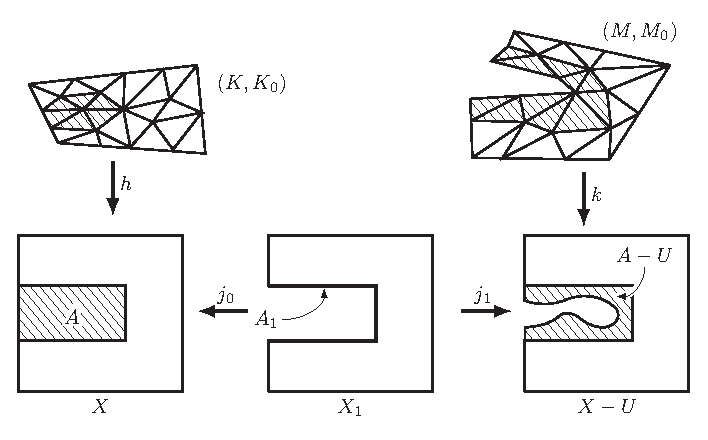
\includegraphics[width=122mm]{figures/3-6-1.pdf}\\图 3.6.1\end{center}
事实上，$|K|\setminus|K_0|$ 是所有 $\sigma\notin K_0$ 的开单形 $\Int\sigma$ 的并，其闭包 $C$ 是由这些单形及其面组成的子复形的多胞体。$h(C)=X_1$，所以 $h$ 剖分 $X_1$，也剖分交集 $A_1$。同样，$|M|\setminus|M_0|$ 的闭包是子复形的多胞体，其像为 $(X\setminus U)\setminus(A\setminus U)=X\setminus A$ 的闭包，即 $X_1$，并同时剖分 $A_1$。这里使用了 $U\subset\Int A$，保证该闭包不接触 $U$。

由已证特殊情形，包含 $j_0:(X_1,A_1)\to(X,A)$ 与 $j_1:(X_1,A_1)\to(X\setminus U,A\setminus U)$ 均诱导同构。因 $j_0=jj_1$，中间包含 $j$ 也诱导同构，完成证明。\hfill$\square$

注意，并未使用完整的切除公理假设：不要求 $\overline U\subset\Int A$，也不要求 $U$ 开。因此有更强结论。

\entry{定理}{3.6.3（单纯理论的切除）}若 $U\subset\Int A\subset X$，且 $(X,A)$ 与 $(X\setminus U,A\setminus U)$ 均可三角剖分，则包含诱导同构 $H_p(X\setminus U,A\setminus U)\cong H_p(X,A)$。

紧支撑公理大致说，每个同调类都有紧支撑。同调类之间的每个同调关系也有紧支撑，精确表述如下。先对单纯理论直接证明，也可由公理导出，见习题。

\entry{定理}{3.6.4}设 $i:(X_0,A_0)\to(X,A)$ 为可三角剖分偶的包含，$(X_0,A_0)$ 紧致。若 $\alpha\in H_p(X_0,A_0)$ 且 $i_*(\alpha)=0$，则存在紧致可三角剖分偶 $(X_1,A_1)$ 及包含 $(X_0,A_0)\xrightarrow{j}(X_1,A_1)\xrightarrow{k}(X,A)$，使 $j_*(\alpha)=0$。

\noindent\textbf{证明：}不妨设 $(X,A)=(|K|,|C|)$。因为 $X_0$ 紧致，包含在某个有限子复形 $K_0$ 的多胞体中；$A_0$ 位于 $|C_0|$，其中 $C_0=C\cap K_0$。故可归结为有限子复形偶的包含 $(K_0,C_0)\to(K,C)$。

取代表 $\alpha$ 的链 $c_p$。其像为零，所以存在 $d_{p+1}$，使 $c_p-\partial d_{p+1}$ 由 $C$ 承载。选 $C$ 的有限子复形承载此差，连同 $C_0$ 取并为 $C_1$。再选 $K$ 的有限子复形承载 $d_{p+1}$，连同 $K_0,C_1$ 取并为 $K_1$。则 $(K_0,C_0)\to(K_1,C_1)$ 已把 $\alpha$ 映到零。\hfill$\square$

\sourcepage{179--180}
\entry{定理}{3.6.5}给定有限生成阿贝尔群序列 $G_0,G_1,\ldots$，其中 $G_0$ 自由且非零，则存在复形 $K$，使每个 $H_i(K)\cong G_i$。

证明留作习题。

\subsection*{习题}
\begin{enumerate}
\item 证明定理 3.6.5。［提示：第 3.4 节习题 5。］
\item 设容许类为所有可三角剖分偶，或所有拓扑空间偶。直接从公理证明定理 3.6.4，其中将“可三角剖分”均换成“容许”。

［提示：可三角剖分情形可以假设 $(X,A)$ 的剖分也剖分 $X_0$。考察图
\begin{center}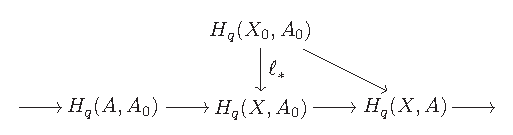
\includegraphics[width=99mm]{figures/3-6-ex-a.pdf}\end{center}
找出紧致 $A_1$，使 $\ell_*(\alpha)$ 位于 $H_q(A_1,A_0)\to H_q(X,A_0)$ 的像中。于是包含 $(X_0,A_0)\to(X,A_1)$ 将 $\alpha$ 映为零。再考察图
\begin{center}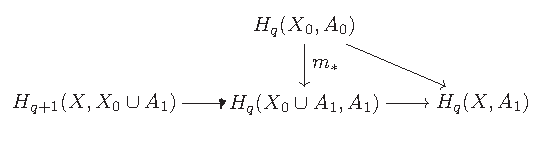
\includegraphics[width=103mm]{figures/3-6-ex-b.pdf}\end{center}
找出紧致 $X_1$，使 $m_*(\alpha)$ 位于 $\partial_*:H_{q+1}(X_1,X_0\cup A_1)\to H_q(X_0\cup A_1,A_1)$ 的像中，然后完成证明。］
\item 给出三个不同的可三角剖分偶的例子。
\end{enumerate}

\section{\texorpdfstring{$*$}{*}范畴与函子}
\sourcepage{180--181}
前面多次提到诱导同态、函子性质，以及将一个数学对象赋给另一个对象的自然性。这些语言背后确有共同思想，本章最后一节研究它。主要是一些新术语，少数证明初等，大多留给读者。

\entry{定义}{3.7.1}\textbf{范畴}（category）$\mathcal C$ 由三部分组成：
\begin{enumerate}[label=(\arabic*)]
\item 一个\textbf{对象}（object）类。
\item 对每个对象有序对 $(X,Y)$，给出\textbf{态射}（morphism）的集合 $\operatorname{hom}(X,Y)$。
\item 对每个对象三元组给出\textbf{复合}运算 $\operatorname{hom}(X,Y)\times\operatorname{hom}(Y,Z)\to\operatorname{hom}(X,Z)$，将 $(f,g)$ 的像记为 $g\circ f$。
\end{enumerate}
要求满足两条公理。

\noindent\textbf{公理 1（结合律）：}若 $f:W\to X$、$g:X\to Y$、$h:Y\to Z$，则 $h\circ(g\circ f)=(h\circ g)\circ f$。

\noindent\textbf{公理 2（恒等态射存在）：}对每个对象 $X$，存在 $1_X\in\operatorname{hom}(X,X)$，使对任意适当的 $f,g$，有 $1_X\circ f=f$、$g\circ1_X=g$。

标准例子是拓扑空间与连续映射，使用通常复合。此例也说明为何说对象构成“类”而不是集合：谈论“所有拓扑空间的集合”或“所有集合的集合”会引出逻辑悖论，例如所有集合的集合是否属于自身？类比集合更大，不对它作通常的集合论运算，例如取所有子集。

恒等态射唯一。若 $1_X,1'_X$ 都满足恒等性质，则 $1_X1'_X=1'_X$，同时 $1_X1'_X=1_X$，所以两者相同。

\entry{定义}{3.7.2}若 $f:X\to Y$、$g,g':Y\to X$，且 $gf=1_X$，称 $g$ 为 $f$ 的\textbf{左逆}；若 $fg'=1_Y$，称 $g'$ 为其\textbf{右逆}。

若同时有左逆、右逆，则由结合律 $g=(g f)g'=g'$，二者相等，称为 $f$ 的\textbf{逆}，并且唯一。有逆的态射称为此范畴中的\textbf{等价态射}（equivalence）。每个态射都可逆的范畴称为\textbf{群胚}（groupoid）。通常以 $f:X\to Y$ 表示 $f\in\operatorname{hom}(X,Y)$，称 $X,Y$ 分别为其定义域对象、值域对象。

\entry{定义}{3.7.3}从范畴 $\mathcal C$ 到 $\mathcal D$ 的\textbf{协变函子}（covariant functor）$G$，给每个对象 $X$ 指定对象 $G(X)$，给每个态射 $f:X\to Y$ 指定态射 $G(f):G(X)\to G(Y)$，满足
\[
G(1_X)=1_{G(X)},\qquad G(g\circ f)=G(g)\circ G(f).
\]
即保持恒等态射与复合。显然，函子把等价态射映为等价态射。

\sourcepage{182--183}
\entry{例}{3.7.4}以下是不同范畴的例子。复合都是通常函数复合或由其诱导；某些等价态射有专名，列于括号中。
\begin{enumerate}[label=(\alph*)]
\item 集合与映射（双射）。
\item 拓扑空间与连续映射（同胚）。
\item 拓扑空间与映射的同伦类（同伦等价）。
\item 单纯复形与单纯映射（单纯同胚）。
\item 单纯复形与其多胞体之间的连续映射。
\item 单纯复形与连续映射的同伦类。
\item 群与同态（同构）。
\item 链复形与链映射。
\item 链复形与链映射的链同伦类（链等价）。
\item 阿贝尔群短正合列与序列同态。
\item 链复形短正合列与序列同态。
\item 阿贝尔群长正合列与序列同态。
\item 拓扑空间的有序对 $(X,Y)$ 与连续映射的有序对 $(f,g)$。
\end{enumerate}

\entry{例}{3.7.5}以下为函子实例。
\begin{enumerate}[label=(\alph*)]
\item 将 $(X,Y)$ 赋为 $X\times Y$，将 $(f,g)$ 赋为 $f\times g$，给出从空间对到空间的函子。
\item 将拓扑空间赋为其底集，将连续映射赋为相同的集合映射，给出从空间到集合的\textbf{遗忘函子}（forgetful functor），它“忘掉”拓扑结构。
\item $K\mapsto\mathcal C(K)$、$f\mapsto f_\#$ 是从单纯复形及单纯映射到链复形及链映射的函子。
\item 给定同调理论，$X\mapsto H_p(X)$、$[h]\mapsto h_*$ 是从容许空间及映射同伦类到阿贝尔群及同态的函子。这正是前两条公理及同伦公理的内容。
\item 之字形引理将链复形短正合列赋为同调长正合列。定理 3.3.3 的自然性正是说，此赋值是函子。
\end{enumerate}

\entry{定义}{3.7.6}设 $G,H:\mathcal C\to\mathcal D$ 为函子。从 $G$ 到 $H$ 的\textbf{自然变换}（natural transformation）$T$，为每个对象指定态射 $T_X:G(X)\to H(X)$，使对每个 $f:X\to Y$，有
\[
\begin{array}{ccc}
G(X)&\xrightarrow{T_X}&H(X)\\
\downarrow\scriptstyle G(f)&&\downarrow\scriptstyle H(f)\\
G(Y)&\xrightarrow{T_Y}&H(Y).
\end{array}
\]
若每个 $T_X$ 都是等价态射，称 $T$ 为函子的\textbf{自然等价}（natural equivalence）。

\entry{例}{3.7.7}固定 $p$，对容许偶定义函子 $G(X,A)=H_p(X,A)$、$G(f)=f_*$，以及 $H(X,A)=H_{p-1}(A)$、$H(f)=(f|_A)_*$。边界与诱导同态的交换性表示 $\partial_*$ 是 $G\to H$ 的自然变换，这恰是第三条 Eilenberg--Steenrod 公理。

\entry{例}{3.7.8}在空间有序对的范畴上，令 $G(X,Y)=X\times Y$、$G(f,g)=f\times g$，$H(X,Y)=Y\times X$、$H(f,g)=g\times f$。交换坐标的同胚 $T_{(X,Y)}$ 给出 $G,H$ 的自然等价。

\sourcepage{184}
至今讨论的是协变函子。还有反变函子，只是“箭头全部反向”。

\entry{定义}{3.7.9}\textbf{反变函子}（contravariant functor）$G:\mathcal C\to\mathcal D$ 给每个对象 $X$ 指定 $G(X)$，给每个 $f:X\to Y$ 指定 $G(f):G(Y)\to G(X)$，满足
\[
G(1_X)=1_{G(X)},\qquad G(g\circ f)=G(f)\circ G(g).
\]
反变函子之间的自然变换按相应方式定义。此前尚未研究反变函子，后面将用到。以线性代数的例子结束本节。

\entry{例}{3.7.10}对实向量空间 $V$，考虑线性泛函空间 $L(V,\R)$，称为 $V$ 的\textbf{对偶空间}。它自然成为向量空间。若 $f:V\to W$ 为线性变换，则有\textbf{转置}或\textbf{伴随}变换 $f^{\mathrm{tr}}:L(W,\R)\to L(V,\R)$：对泛函 $\alpha:W\to\R$，令 $f^{\mathrm{tr}}(\alpha)=\alpha\circ f$。赋值 $V\mapsto L(V,\R)$、$f\mapsto f^{\mathrm{tr}}$ 为向量空间与线性变换范畴到自身的反变函子。

\sourcepage{184--186}
\subsection*{习题}
\begin{enumerate}
\item 验证例 3.7.4 的对象与态射确实构成范畴，且等价态射如所述。［只有 (c)、(i) 需要特别注意。］
\item 此前学过的数学中已出现许多函子，只是未必使用此名称。回顾以下例子。
\begin{enumerate}[label=(\alph*)]
\item 对复形与单纯映射等价类的范畴，其中等价关系由邻接关系生成，定义到链复形与链同伦类范畴的函子。
\item 给出从抽象复形到几何复形的“几何实现函子”，并说明涉及的映射。
\item 对固定指标集 $J$ 编号的阿贝尔群族，给出到阿贝尔群的“直积”与“直和”函子。
\item 回顾或查阅代数中的“阿贝尔化函子” $G\mapsto G/[G,G]$。
\item 回顾或查阅从完全正则空间到紧致 Hausdorff 空间的 Stone--Čech 紧化函子。不要只处理空间，还须处理映射。
\end{enumerate}
\item 设 $G,H$ 分别将复形赋为定向链复形、有序链复形，将单纯映射赋为诱导链映射。
\begin{enumerate}[label=(\alph*)]
\item $G\to H$ 或 $H\to G$ 中有一个方向存在自然变换，确定方向。
\item 若值范畴改为链复形与链映射的链同伦类，证明两个方向都存在自然变换，而且都是自然等价。
\end{enumerate}
\item 考虑空间对 $(X,Y)$，其中两者及乘积均可三角剖分，态射为连续映射对。定义 $G(X,Y)=H_p(X\times Y)$、$G(f,g)=(f\times g)_*$，$H(X,Y)=H_p(X)\times H_p(Y)$、$H(f,g)=f_*\times g_*$。构造自然变换 $G\to H$，证明它不是自然等价。
\item 此前的态射都是映射或映射等价类。以下例子供熟悉基本群的读者考虑。固定空间 $X$，以其点为对象，以从 $x_0$ 到 $x_1$ 的道路的道路同伦类组成 $\operatorname{hom}(x_1,x_0)$。道路复合 $(\beta,\alpha)\mapsto\alpha*\beta$ 诱导态射复合。
\begin{enumerate}[label=(\alph*)]
\item 验证它是群胚。
\item 验证 $x_0\mapsto\pi_1(X,x_0)$、$[\alpha]\mapsto\widehat\alpha$ 为到群及同态范畴的反变函子，其中 $\widehat\alpha([f])=[\alpha*f*\overline\alpha]$，$\overline\alpha$ 为反向道路。［把 $[\alpha]$ 放在 $\operatorname{hom}(x_1,x_0)$ 而非相反方向，是因为道路复合把先走的道路写在左边，而函数复合把先作用的函数写在右边。］
\end{enumerate}
\item 举出一个在阿贝尔群背景中出现的反变函子。
\end{enumerate}

\chapter{奇异同调论}
\section{引言}
\sourcepage{187}
现在，在某种意义上要重新开始，构造一种新的同调理论。与单纯理论相比，它“自然”得多：同调群对任意拓扑空间都有定义，而不只对可三角剖分空间；连续映射的诱导同态可直接定义，函子性质也容易证明，不需要单纯逼近定理等困难结果。奇异同调群的拓扑不变性立即得到。

遗憾的是，奇异同调群不能立即计算。即使对于 $S^n$ 这样简单的空间，也需要发展相当多的理论才能计算。最终研究 CW 复形时，将看到如何比较方便地计算奇异同调。另一方面，我们将证明可三角剖分空间的单纯同调与奇异同调同构，所以要计算时，总可以回到单纯理论。

本章构造奇异同调群，并证明它们在全部拓扑空间类上满足 Eilenberg--Steenrod 公理；其中同伦与切除公理比其他公理需要更多工作。然后构造奇异理论与单纯理论之间的具体同构，供后文使用。

最后给出许多应用，包括 Jordan 曲线定理、流形的相关定理，以及实射影空间与复射影空间的同调计算。

\section{奇异同调群}
\sourcepage{187--188}
本节定义奇异同调群，并建立它们的一些初等性质。先引入记号。

以 $\R^\infty$ 表示 $E^J$，其中 $J=\Z_+$ 是正整数集；它的点是只有有限个非零项的实数序列。记 $\epsilon_0=0$，并以 $\epsilon_1,\epsilon_2,\ldots$ 表示通常的基向量。由 $\epsilon_0,\ldots,\epsilon_p$ 张成的单形称为\textbf{标准 $p$ 维单形}（standard $p$-simplex），记作 $\Delta_p$。于是 $\Delta_{p-1}$ 是 $\Delta_p$ 的一个面。

拓扑空间 $X$ 中的一个\textbf{奇异 $p$ 维单形}（singular $p$-simplex）是连续映射 $T:\Delta_p\to X$。这里的映射不必是嵌入，甚至可以是常值映射。以 $S_p(X)$ 表示以所有奇异 $p$ 维单形为基的自由阿贝尔群，称为 $X$ 的 $p$ 维\textbf{奇异链群}（singular chain group）。它的元素称为奇异 $p$ 维链，是奇异单形的有限整数线性组合。

若 $a_0,\ldots,a_p$ 是 $E^J$ 中任意一些点（不要求几何独立），则存在唯一的仿射映射 $\Delta_p\to E^J$，将 $\epsilon_i$ 映至 $a_i$。称它为\textbf{线性奇异单形}（linear singular simplex），记作 $\ell(a_0,\ldots,a_p)$。具体地，
\[
\ell(a_0,\ldots,a_p)(x_1,\ldots,x_p,0,\ldots)
=a_0+\sum_{i=1}^p x_i(a_i-a_0).
\]
\translatornote{原书此处求和上限印为 $n$；按所定义的 $p$ 维单形，应为 $p$。}
特别地，$\ell(\epsilon_0,\ldots,\epsilon_p)$ 是 $\Delta_p$ 到 $\R^\infty$ 的包含映射。而
\[
\ell(\epsilon_0,\ldots,\widehat\epsilon_i,\ldots,\epsilon_p):\Delta_{p-1}\longrightarrow\Delta_p
\]
将 $\Delta_{p-1}$ 线性同胚地映到 $\Delta_p$ 的第 $i$ 个面。将它与 $T$ 复合，所得奇异 $(p-1)$ 维单形称为 $T$ 的第 $i$ 个面。

\sourcepage{189}
定义\textbf{边缘算子} $\partial:S_p(X)\to S_{p-1}(X)$：在基元上令
\[
\partial T=\sum_{i=0}^p(-1)^iT\circ\ell(\epsilon_0,\ldots,\widehat\epsilon_i,\ldots,\epsilon_p),
\]
再线性延拓。\translatornote{原书这一定义中的符号印为 $(-1)^p$；应为随面指标交替的 $(-1)^i$。}若 $f:X\to Y$ 连续，则定义同态 $f_\#:S_p(X)\to S_p(Y)$，使 $f_\#T=f\circ T$。

\entry{定理}{4.2.1}同态 $f_\#$ 与 $\partial$ 可交换，并且 $\partial^2=0$。

\textbf{证明：}对任一奇异单形 $T$，
\begin{align*}
\partial f_\#T&=\sum_{i=0}^p(-1)^i(f\circ T)\circ\ell(\epsilon_0,\ldots,\widehat\epsilon_i,\ldots,\epsilon_p),\\
f_\#\partial T&=\sum_{i=0}^p(-1)^if\circ\bigl(T\circ\ell(\epsilon_0,\ldots,\widehat\epsilon_i,\ldots,\epsilon_p)\bigr).
\end{align*}
两者由复合的结合律相等。对于线性奇异单形，线性映射的复合仍为线性映射，因而
\[
\partial\ell(a_0,\ldots,a_p)=\sum_{i=0}^p(-1)^i\ell(a_0,\ldots,\widehat a_i,\ldots,a_p).
\]
像引理 1.6.9 的证明一样展开两次边缘，每一项出现两次，符号相反，故在线性奇异单形上 $\partial^2=0$。对一般的 $T$，注意
\[
T=T_\#\bigl(\ell(\epsilon_0,\ldots,\epsilon_p)\bigr).
\]
由刚证明的交换性，$\partial^2T=T_\#\partial^2\ell(\epsilon_0,\ldots,\epsilon_p)=0$。\hfill$\square$

\sourcepage{190}
\entry{定义}{4.2.2}群 $S_p(X)$ 连同边缘算子构成的链复形记为 $\mathcal S(X)$，称为 $X$ 的\textbf{奇异链复形}（singular chain complex）。它的同调群称为 $X$ 的\textbf{奇异同调群}（singular homology groups），记为 $H_p(X)$。这一记号与第 3.6 节的单纯同调群相同；第 4.7 节将证明两者之间有自然同构。

定义增广同态 $\epsilon:S_0(X)\to\Z$，将每个奇异零维单形映为 $1$。对于奇异一维单形 $T$，有 $\epsilon\partial T=0$，所以可定义约化奇异同调群 $\widetilde H_p(X)$。映射 $f_\#$ 保持增广，故在普通及约化同调群上都诱导同态 $f_*$。若所有约化奇异同调群都为零，称 $X$ \textbf{无环}。

\entry{定理}{4.2.3}恒等映射诱导恒等同态；若 $f:X\to Y$、$g:Y\to Z$ 连续，则 $(g\circ f)_*=g_*\circ f_*$。这对普通及约化奇异同调均成立。

\textbf{证明：}这些等式在链的层次上已经成立：$i_\#T=T$，且 $(g\circ f)_\#T=g_\#f_\#T$。\hfill$\square$

\entry{推论}{4.2.4}若 $h:X\to Y$ 是同胚，则 $h_*$ 是同构。

因此，奇异同调群的拓扑不变性立刻得到；与第二章中证明单纯同调群拓扑不变性所需的工作相比，这一点十分显著。

\entry{定理}{4.2.5}在 $X$ 的每个道路分支 $X_\alpha$ 中选取一个奇异零维单形 $T_\alpha$。则 $H_0(X)$ 是自由阿贝尔群，以诸 $T_\alpha$ 的同调类为基。群 $\widetilde H_0(X)$ 也是自由阿贝尔群：若 $X$ 道路连通，它为零；否则，固定 $\alpha_0$，则诸 $T_\alpha-T_{\alpha_0}$（$\alpha\ne\alpha_0$）的同调类构成一组基。

\sourcepage{191}
\textbf{证明：}设奇异零维单形 $T$ 的像为点 $x\in X_\alpha$。从 $x$ 到 $T_\alpha(\Delta_0)$ 的一条道路 $f:[0,1]\to X$ 是奇异一维单形，且 $\partial f=T_\alpha-T$。故每个零维链均同调于某个有限和 $\sum n_\alpha T_\alpha$。

若 $\sum n_\alpha T_\alpha=\partial d$，每个奇异一维单形的像道路连通，因而完全包含于某个 $X_\alpha$。可相应写成 $d=\sum d_\alpha$，其中 $d_\alpha\in S_1(X_\alpha)$。比较各道路分支内的基元，得 $n_\alpha T_\alpha=\partial d_\alpha$。施以增广，得 $n_\alpha=0$。这证明了线性无关性。\translatornote{原书在此还说“因此 $d=0$”；这个结论一般不成立，因为 $d$ 可以是非零闭链。实际所需且已经证明的是所有 $n_\alpha=0$。}关于约化同调的结论，用与定理 1.8.3 相同的论证即可得到。\hfill$\square$

下面把星形凸性的概念推广到 $E^J$ 的子空间。

\entry{定义}{4.2.6}若 $w\in X\subset E^J$，且连接 $X$ 中每个点与 $w$ 的线段都包含于 $X$，则称 $X$ \textbf{关于 $w$ 星形凸}（star convex relative to $w$）。

\entry{定义}{4.2.7}设 $X$ 关于 $w$ 星形凸，$T:\Delta_p\to X$ 为奇异单形。定义 $[T,w]:\Delta_{p+1}\to X$：对于 $x\in\Delta_p$，将从 $x$ 到 $\epsilon_{p+1}$ 的线段线性地映到从 $T(x)$ 到 $w$ 的线段。对链 $c=\sum n_iT_i$，令 $[c,w]=\sum n_i[T_i,w]$。这与第 1.9 节的括号运算类似，不过顶点现在写在末尾。

映射 $[T,w]$ 在 $\Delta_p$ 上的限制为 $T$。若 $T=\ell(a_0,\ldots,a_p)$，则 $[T,w]=\ell(a_0,\ldots,a_p,w)$。

为证明连续性，考虑商映射
\[
\pi:\Delta_p\times I\to\Delta_{p+1},\qquad \pi(x,t)=(1-t)x+t\epsilon_{p+1},
\]
它把 $\Delta_p\times\{1\}$ 压缩为一点。连续映射 $f(x,t)=(1-t)T(x)+tw$ 在该集合上为常值，故通过 $\pi$ 诱导一个从 $\Delta_{p+1}$ 到 $X$ 的连续映射。\translatornote{原书将此处的常值集合写为 $\Delta_p$；应为 $\Delta_p\times\{1\}$。}

\sourcepage{192}
\begin{center}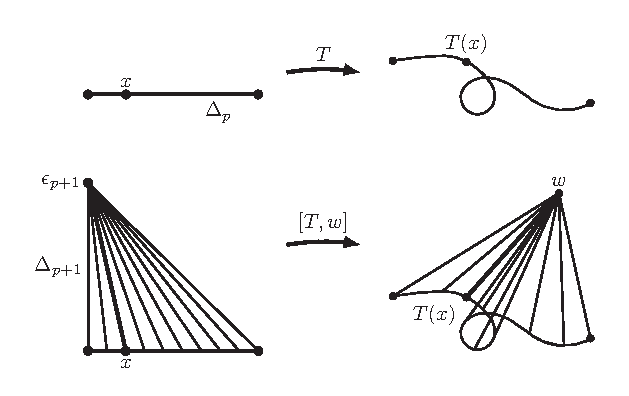
\includegraphics[width=.87\textwidth]{figures/4-2-1.pdf}\\图 4.2.1\end{center}
由于 $\pi$ 将 $\{x\}\times I$ 线性地映到从 $x$ 到 $\epsilon_{p+1}$ 的线段，而 $f$ 将它线性地映到从 $T(x)$ 到 $w$ 的线段，这个诱导映射恰好是 $[T,w]$。因此 $[T,w]$ 连续。现在计算括号运算与边缘算子的关系。

\entry{引理}{4.2.8}设 $X$ 关于 $w$ 星形凸，$c$ 是 $X$ 中的奇异 $p$ 维链，则
\[
\partial[c,w]=\begin{cases}[\partial c,w]+(-1)^{p+1}c,&p>0,\\\epsilon(c)T_w-c,&p=0,\end{cases}
\]
其中 $T_w$ 是将 $\Delta_0$ 映到 $w$ 的奇异零维单形。

\textbf{证明：}若 $T$ 为零维单形，则 $[T,w]$ 将 $\Delta_1$ 线性地映到从 $T(\Delta_0)$ 到 $w$ 的线段，所以 $\partial[T,w]=T_w-T$。由线性性得第二个公式。

设 $p>0$。只需对奇异 $p$ 维单形 $T$ 验证第一个公式。图 4.2.2 说明了 $p=1$ 的情形。由定义，
\[
\partial[T,w]=\sum_{i=0}^{p+1}(-1)^i[T,w]\circ\ell(\epsilon_0,\ldots,\widehat\epsilon_i,\ldots,\epsilon_{p+1}).\tag{*}
\]
\sourcepage{193}
简记 $\ell_i=\ell(\epsilon_0,\ldots,\widehat\epsilon_i,\ldots,\epsilon_{p+1})$。
\begin{center}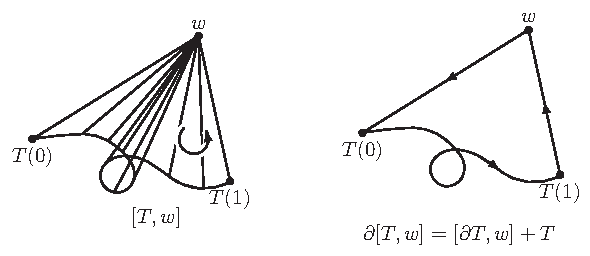
\includegraphics[width=.85\textwidth]{figures/4-2-2.pdf}\\图 4.2.2\end{center}
映射 $\ell_{p+1}$ 是 $\Delta_p$ 到 $\Delta_{p+1}$ 的包含映射，而 $[T,w]|_{\Delta_p}=T$，故式 (*) 的末项为 $(-1)^{p+1}T$。

再考虑 $i<p+1$。映射 $\ell_i$ 将 $\Delta_p$ 线性同胚地映到 $\Delta_{p+1}$ 的第 $i$ 个面，并将顶点 $\epsilon_0,\ldots,\epsilon_p$ 依次映到 $\epsilon_0,\ldots,\widehat\epsilon_i,\ldots,\epsilon_{p+1}$。所以其在 $\Delta_{p-1}$ 上的限制满足
\[
\ell_i|_{\Delta_{p-1}}=\ell(\epsilon_0,\ldots,\widehat\epsilon_i,\ldots,\epsilon_p).\tag{**}
\]
对于 $x\in\Delta_{p-1}$，$\ell_i$ 将从 $x$ 到 $\epsilon_p$ 的线段线性地映到从 $\ell_i(x)$ 到 $\epsilon_{p+1}$ 的线段。因为 $\ell_i(x)\in\Delta_p$，$[T,w]$ 又将后一线段线性地映到从 $T(\ell_i(x))$ 到 $w$ 的线段。因此，
\[
[T,w]\circ\ell_i=[T\circ(\ell_i|_{\Delta_{p-1}}),w].
\]
\translatornote{原书此等式左端漏印了复合映射 $\circ\ell_i$。}代入 (*) 并使用 (**)，得
\begin{align*}
\partial[T,w]&=\sum_{i=0}^{p}(-1)^i[T\circ\ell(\epsilon_0,\ldots,\widehat\epsilon_i,\ldots,\epsilon_p),w]+(-1)^{p+1}T\\
&=[\partial T,w]+(-1)^{p+1}T.
\end{align*}
\hfill$\square$

\entry{定理}{4.2.9}若 $X\subset E^J$ 关于 $w$ 星形凸，则 $X$ 的奇异同调无环。

\sourcepage{194}
\textbf{证明：}若零维链 $c$ 满足 $\epsilon(c)=0$，则上述引理给出 $\partial[c,w]=\epsilon(c)T_w-c=-c$，故 $c$ 是边缘，$\widetilde H_0(X)=0$。若 $z$ 是 $p>0$ 维闭链，则
\[
\partial[z,w]=[\partial z,w]+(-1)^{p+1}z=(-1)^{p+1}z,
\]
故 $z$ 也是边缘，$H_p(X)=0$。\hfill$\square$

\entry{推论}{4.2.10}任意单形的奇异同调无环。

\entry{定义}{4.2.11}图 4.2.3 中的\textbf{拓扑学家的正弦曲线}（topologist's sine curve）是 $\R^2$ 的子空间
\[
Y=\{(x,\sin(1/x)):0<x\le1\}\cup\{(0,y):-1\le y\le1\}.
\]
习题 1(b) 将用到这个空间。
\begin{center}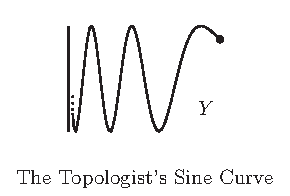
\includegraphics[width=.48\textwidth]{figures/4-2-3.pdf}\\图 4.2.3：拓扑学家的正弦曲线\end{center}

\subsection*{习题}
\begin{enumerate}
\item \begin{enumerate}[label=(\alph*)]
\item 设 $\{X_\alpha\}$ 是 $X$ 的道路分支全体。证明 $H_p(X)\cong\bigoplus_\alpha H_p(X_\alpha)$。
\item 计算拓扑学家的正弦曲线 $Y$ 的奇异同调。
\end{enumerate}
\item 设 $X$ 是 $\R^N$ 的紧子空间，$f:X\to Y$。
\begin{enumerate}[label=(\alph*)]
\item 设 $w=(0,0,\ldots,0,1)\in\R^N\times\R$，$C$ 是连接 $X$ 中各点与 $w$ 的所有线段之并。证明 $C$ 是 $X\times I$ 的商空间。
\item 证明：若 $f$ 同伦于常值映射，则在约化同调中 $f_*$ 是零同态。〔提示：证明 $f$ 可以延拓到 $C$。〕
\item 证明：若 $X$ 可缩，则 $X$ 无环。
\end{enumerate}
\item 计算 $\R^2$ 中单位圆盘的 $H_1$。
\item 证明：若 $U\subset\R^2$ 同胚于单位圆盘，则对每个 $p>0$，都有 $H_p(U)=0$。
\end{enumerate}

\section{奇异同调论的公理}
\sourcepage{195}
现在引入相对奇异同调群。本节及下一节将证明，它们在所有拓扑空间偶构成的类上满足 Eilenberg--Steenrod 公理。

若 $A$ 是拓扑空间 $X$ 的子空间，则有自然的包含映射 $S_p(A)\to S_p(X)$。定义\textbf{相对奇异链群}
\[
S_p(X,A)=S_p(X)/S_p(A).
\]
边缘算子 $S_p(X)\to S_{p-1}(X)$ 在 $S_p(A)$ 上的限制正是该子空间的边缘算子，故诱导相对链上的边缘算子
\[
\partial:S_p(X,A)\to S_{p-1}(X,A).
\]
这些群和同态组成\textbf{空间偶 $(X,A)$ 的奇异链复形}，记作 $\mathcal S(X,A)$。其同调群称为\textbf{空间偶 $(X,A)$ 的奇异同调群}，记作 $H_p(X,A)$。

链复形 $\mathcal S(X,A)$ 是自由的：$S_p(X,A)$ 的一组基由所有形如 $T+S_p(A)$ 的陪集组成，其中 $T$ 是像不完全包含于 $A$ 的奇异 $p$ 维单形。

若 $f:(X,A)\to(Y,B)$ 连续，则 $f_\#:S_p(X)\to S_p(Y)$ 将 $A$ 中的链映为 $B$ 中的链，故诱导同态
\[
f_\#:S_p(X,A)\to S_p(Y,B).
\]
它与 $\partial$ 可交换，进而诱导 $f_*:H_p(X,A)\to H_p(Y,B)$。下面的结论是直接的。

\entry{定理}{4.3.1}若 $i:(X,A)\to(X,A)$ 是恒等映射，则 $i_*:H_p(X,A)\to H_p(X,A)$ 是恒等同态。若 $h:(X,A)\to(Y,B)$、$k:(Y,B)\to(Z,C)$ 连续，则 $(k\circ h)_*=k_*\circ h_*$。\translatornote{原书第一句中的同调群漏印了相对子空间 $A$。}

\sourcepage{196}
\entry{定理}{4.3.2}对 $A\subset X$ 及每个 $p$，存在同态 $\partial_*:H_p(X,A)\to H_{p-1}(A)$，使序列
\[
\cdots\longrightarrow H_p(A)\xrightarrow{i_*}H_p(X)\xrightarrow{\pi_*}H_p(X,A)\xrightarrow{\partial_*}H_{p-1}(A)\longrightarrow\cdots
\]
正合，其中 $i$、$\pi$ 均为包含映射。若 $A\ne\varnothing$，对 $X$ 和 $A$ 采用约化同调时亦然。连续映射 $f:(X,A)\to(Y,B)$ 在普通或约化奇异同调中，都诱导相应长正合列之间的同态。

\textbf{证明：}对链复形的短正合列
\[
0\longrightarrow S_p(A)\xrightarrow{i_\#}S_p(X)\xrightarrow{\pi_\#}S_p(X,A)\longrightarrow0
\]
应用“之字形引理”（引理 3.3.2），即得 $\partial_*$ 及长正合列。其中 $i:A\to X$、$\pi:(X,\varnothing)\to(X,A)$ 是包含映射。注意 $f_\#$ 与 $i_\#$、$\pi_\#$ 可交换，故由定理 3.3.3 得 $\partial_*$ 的自然性。约化同调的结论可用引理 3.3.5 中处理单纯同调的同样方法证明。\hfill$\square$

\entry{定理}{4.3.3}若 $P$ 是单点空间，则 $p\ne0$ 时 $H_p(P)=0$，而 $H_0(P)=\Z$。

\textbf{证明：}$\R^N$ 中的单点空间关于其唯一的点星形凸，故可直接应用定理 4.2.9。

也可以作如下显式计算。在每个非负维数恰有一个奇异单形 $T_p:\Delta_p\to P$，所以 $p\ge0$ 时 $S_p(P)$ 为无限循环群。由于
\[
T_p\circ\ell(\epsilon_0,\ldots,\widehat\epsilon_i,\ldots,\epsilon_p)=T_{p-1},
\]
对 $p>0$ 有
\[
\partial T_p=\sum_{i=0}^p(-1)^iT_{p-1}
=\begin{cases}0,&p\text{ 为奇数},\\T_{p-1},&p\text{ 为偶数}.\end{cases}
\]
因此链复形 $\mathcal S(P)$ 具有如下形式：
\[
\cdots\xrightarrow{0}\Z\xrightarrow{\cong}\Z\xrightarrow{0}\Z\xrightarrow{\cong}\Z\xrightarrow{0}\Z\longrightarrow0,
\]
其中最右边的 $\Z$ 在零维。奇数维中每个链都是边缘；正偶数维中没有非零闭链；零维中每个链都是闭链，而没有非零边缘。因此零维同调为无限循环群，其余维数均为零。\hfill$\square$

\sourcepage{197}
\entry{定理}{4.3.4}给定 $\alpha\in H_p(X,A)$，存在紧空间偶 $(X_0,A_0)\subset(X,A)$，使 $\alpha$ 属于包含映射诱导的同态
\[
i_*:H_p(X_0,A_0)\to H_p(X,A)
\]
的像。

\textbf{证明：}奇异单形 $T:\Delta_p\to X$ 的\textbf{最小载体}定义为像集 $T(\Delta_p)$。链 $\sum n_iT_i$（每个 $n_i\ne0$）的最小载体是诸 $T_i$ 的最小载体之并。因为这个和有限，链的最小载体是紧的。

取 $c_p\in S_p(X)$，使其模 $S_p(A)$ 的陪集代表 $\alpha$。则 $\partial c_p$ 的载体在 $A$ 内。令 $X_0$ 是 $c_p$ 的最小载体，$A_0$ 是 $\partial c_p$ 的最小载体。于是 $c_p$ 代表 $H_p(X_0,A_0)$ 中的一个类 $\beta$，且 $i_*(\beta)=\alpha$。\hfill$\square$

上述定理说明奇异同调论满足紧支集公理。下面证明它的一个补充结论。〔也可直接由公理导出，见第 3.6 节习题。〕

\entry{定理}{4.3.5}设 $(X_0,A_0)$ 为紧空间偶，$i:(X_0,A_0)\to(X,A)$ 为包含映射。若 $\alpha\in H_p(X_0,A_0)$ 且 $i_*(\alpha)=0$，则存在紧空间偶 $(X_1,A_1)$ 及包含映射
\[
(X_0,A_0)\xrightarrow{j}(X_1,A_1)\xrightarrow{k}(X,A),
\]
使 $j_*(\alpha)=0$。

\textbf{证明：}设 $X_0$ 中的奇异链 $c_p$ 代表 $\alpha$，则 $\partial c_p$ 的载体在 $A_0$ 内。由假设，存在 $X$ 中的链 $d_{p+1}$，使 $c_p-\partial d_{p+1}$ 的载体在 $A$ 内。令 $X_1$ 为 $X_0$ 与 $d_{p+1}$ 的最小载体之并，$A_1$ 为 $A_0$ 与 $c_p-\partial d_{p+1}$ 的最小载体之并，即得所求。\hfill$\square$

到目前为止的工作都比较容易。除同伦公理与切除公理外，其余公理均已验证。后两条需要更多工作。现在证明同伦公理，切除公理留待下一节。

证明的轮廓与单纯同调的同伦公理证明（定理 2.7.5）相似。考虑 $i,j:X\to X\times I$，其中 $i(x)=(x,0)$、$j(x)=(x,1)$，构造 $i_\#$ 与 $j_\#$ 之间的链同伦 $D$。若 $F$ 是 $f$ 与 $g$ 之间的同伦，则 $F_\#\circ D$ 是 $f_\#$ 与 $g_\#$ 之间的链同伦，结论随即成立。

\sourcepage{198}
单纯同调中曾用无环载体构造 $D$；这里需要一种更一般的方法，它是后面所谓“无环模型法”（method of acyclic models）的一个特例。

这样的 $D$ 应当存在，是很直观的。例如图 4.3.1 中的奇异一维单形 $T$ 满足 $\partial T=T_1-T_0$。可取 $DT_1$、$DT_0$ 为图中“竖直”的奇异一维单形，再取覆盖阴影区域的二维链作为 $DT$，使其边缘为 $j_\#T-DT_1-i_\#T+DT_0$。
\begin{center}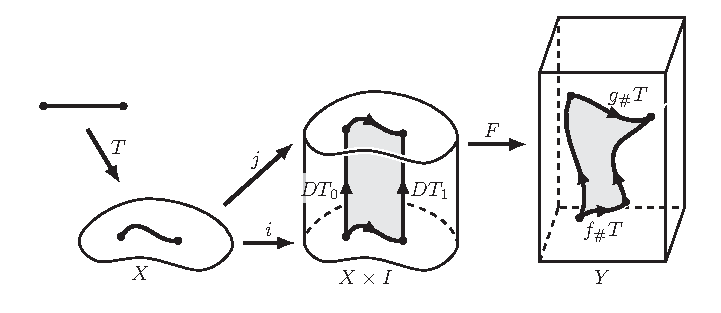
\includegraphics[width=.96\textwidth]{figures/4-3-1.pdf}\\图 4.3.1\end{center}
将 $D$ 的存在性单列为引理。

\entry{引理}{4.3.6}对每个空间 $X$ 及每个非负整数 $p$，存在同态
\[
D_X:S_p(X)\to S_{p+1}(X\times I),
\]
具有下列性质：
\begin{enumerate}[label=(\alph*)]
\item 对每个奇异单形 $T:\Delta_p\to X$，有 $\partial D_XT+D_X\partial T=j_\#T-i_\#T$，其中 $i(x)=(x,0)$、$j(x)=(x,1)$。
\item $D_X$ 具有自然性：若 $f:X\to Y$ 连续，则下图交换（$i_I$ 为 $I$ 的恒等映射）：
\[
\begin{array}{ccc}
S_p(X)&\xrightarrow{D_X}&S_{p+1}(X\times I)\\
\downarrow\scriptstyle f_\#&&\downarrow\scriptstyle(f\times i_I)_\#\\
S_p(Y)&\xrightarrow{D_Y}&S_{p+1}(Y\times I).
\end{array}
\]
\end{enumerate}

\sourcepage{199}
\textbf{证明：}对 $p$ 归纳。先设 $p=0$。给定 $T:\Delta_0\to X$，以 $x_0$ 表示 $T(\Delta_0)$，定义
\[
D_XT(t,0,0,\ldots)=(x_0,t)\qquad(0\le t\le1).
\]
〔回忆 $\Delta_1=\epsilon_0\epsilon_1$ 正是所有这种形式的点组成的线段。〕性质 (a)、(b) 易于验证。

现设 $p>0$，并假定对所有空间，在小于 $p$ 的维数上都已定义满足 (a)、(b) 的 $D_X$。先在特殊情形 $X=\Delta_p$、$T=i_p$ 下定义 $D_XT$，其中 $i_p$ 为 $\Delta_p$ 的恒等映射。这正是方法的核心：先处理一个称为“模型空间”的特殊空间，以及其上一个特殊奇异单形。

令 $\widehat i,\widehat j:\Delta_p\to\Delta_p\times I$ 分别将 $x$ 映到 $(x,0)$、$(x,1)$。定义 $\Delta_p\times I$ 上的奇异链
\[
c_p=\widehat j_\#(i_p)-\widehat i_\#(i_p)-D_{\Delta_p}(\partial i_p).
\]
因为 $i_p\in S_p(\Delta_p)$，而 $\partial i_p\in S_{p-1}(\Delta_p)$，归纳假设保证最后一项已有定义。再由归纳假设，
\begin{align*}
\partial c_p&=\partial\widehat j_\#(i_p)-\partial\widehat i_\#(i_p)-\partial D_{\Delta_p}(\partial i_p)\\
&=\widehat j_\#(\partial i_p)-\widehat i_\#(\partial i_p)
-\bigl[\widehat j_\#(\partial i_p)-\widehat i_\#(\partial i_p)-D_{\Delta_p}\partial\partial i_p\bigr]=0.
\end{align*}
空间 $\Delta_p\times I$ 为凸集，由定理 4.2.9 无环。所以可选 $S_{p+1}(\Delta_p\times I)$ 中一个边缘为 $c_p$ 的元素，记为 $D_{\Delta_p}(i_p)$。于是
\[
\partial D_{\Delta_p}(i_p)=\widehat j_\#(i_p)-\widehat i_\#(i_p)-D_{\Delta_p}(\partial i_p),
\]
即满足 (a)。

对任意空间 $X$ 和任意奇异单形 $T:\Delta_p\to X$，定义
\[
D_XT=(T\times i_I)_\#\bigl(D_{\Delta_p}i_p\bigr),
\]
并线性延拓。见图 4.3.2。直观地，$D_{\Delta_p}i_p$ 是填满棱柱 $\Delta_p\times I$ 的奇异 $(p+1)$ 维链，其边缘大致就是棱柱的边缘；$(T\times i_I)_\#$ 将这个链映到 $X\times I$。

验证 (a)，计算得
\begin{align*}
\partial D_XT&=(T\times i_I)_\#\partial D_{\Delta_p}i_p\\
&=(T\times i_I)_\#\bigl(\widehat j_\#i_p-\widehat i_\#i_p-D_{\Delta_p}\partial i_p\bigr)\\
&=j_\#T-i_\#T-(T\times i_I)_\#D_{\Delta_p}(\partial i_p).\tag{*}
\end{align*}
\sourcepage{200}
\begin{center}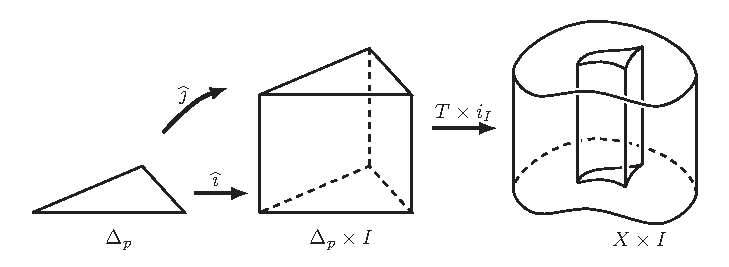
\includegraphics[width=.96\textwidth]{figures/4-3-2.pdf}\\图 4.3.2\end{center}
由低一维的自然性归纳假设，下图交换：
\[
\begin{array}{ccc}
S_{p-1}(\Delta_p)&\xrightarrow{D_{\Delta_p}}&S_p(\Delta_p\times I)\\
\downarrow\scriptstyle T_\#&&\downarrow\scriptstyle(T\times i_I)_\#\\
S_{p-1}(X)&\xrightarrow{D_X}&S_p(X\times I).
\end{array}
\]
故 $(T\times i_I)_\#D_{\Delta_p}(\partial i_p)=D_XT_\#(\partial i_p)=D_X\partial T$，式 (*) 正是所求。

验证 (b) 更为直接。若 $f:X\to Y$，则 $(f\circ T)\times i_I=(f\times i_I)\circ(T\times i_I)$。由定义，
\begin{align*}
D_Y(f_\#T)&=D_Y(f\circ T)=((f\circ T)\times i_I)_\#D_{\Delta_p}(i_p)\\
&=((f\times i_I)\circ(T\times i_I))_\#D_{\Delta_p}(i_p)=(f\times i_I)_\#D_XT.
\end{align*}

上述证明在 $p=0$ 时直接构造 $D_X$，只在归纳步骤中用了模型空间。下面给出一个更像归纳步骤的零维证明；后面将推广的正是这种证明。

先对 $X=\Delta_0$、$T=i_0$ 定义 $D_XT$。所需等式为
\[
\partial D_{\Delta_0}(i_0)=\widehat j_\#(i_0)-\widehat i_\#(i_0).
\]
右端是 $\Delta_0\times I$ 中增广为零的零维链。该空间为凸集，故无环；可选择一个一维链 $D_{\Delta_0}(i_0)$，使其边缘为右端。对于一般的 $X$ 和 $T$，令 $D_XT=(T\times i_I)_\#D_{\Delta_0}(i_0)$。性质 (a)、(b) 的证明与归纳步骤完全相同。\hfill$\square$

\sourcepage{201}
\entry{定理}{4.3.7}若 $f,g:(X,A)\to(Y,B)$ 同伦，则 $f_*=g_*$。当 $A=B=\varnothing$ 时，约化同调也有同样结论。

\textbf{证明：}设 $F:(X\times I,A\times I)\to(Y,B)$ 是从 $f$ 到 $g$ 的同伦，$i(x)=(x,0)$、$j(x)=(x,1)$。由 $D_X$ 对包含映射 $A\to X$ 的自然性，其在 $S_p(A)$ 上的限制为 $D_A$。所以 $D_X$ 将 $S_p(A)$ 映入 $S_{p+1}(A\times I)$，在相对链上诱导
\[
D_{X,A}:S_p(X,A)\to S_{p+1}(X\times I,A\times I),
\]
并满足引理 4.3.6(a) 的公式。令 $D=F_\#D_{X,A}$，其中
\[
F_\#:S_{p+1}(X\times I,A\times I)\to S_{p+1}(Y,B).
\]
于是
\begin{align*}
\partial D&=F_\#\partial D_{X,A}=F_\#(j_\#-i_\#-D_{X,A}\partial)\\
&=(F\circ j)_\#-(F\circ i)_\#-D\partial=g_\#-f_\#-D\partial.
\end{align*}
故 $f_\#$ 与 $g_\#$ 链同伦。\translatornote{原书最后一行写为 $f_\#-g_\#-D\partial$；若同伦按 $F(x,0)=f(x)$、$F(x,1)=g(x)$ 约定，则应如上。结论不受此符号笔误影响。}\hfill$\square$

\entry{定义}{4.3.8}设 $f:(X,A)\to(Y,B)$。若存在 $g:(Y,B)\to(X,A)$，使 $f\circ g$、$g\circ f$ 作为空间偶的映射分别同伦于相应恒等映射，则称 $f$ 为\textbf{同伦等价}，$g$ 为 $f$ 的\textbf{同伦逆}。

\entry{定理}{4.3.9}设 $f:(X,A)\to(Y,B)$。
\begin{enumerate}[label=(\alph*)]
\item 若 $f$ 为同伦等价，则 $f_*$ 在相对同调中为同构。
\item 更一般地，若 $f:X\to Y$ 与 $f|_A:A\to B$ 都是同伦等价，则 $f_*$ 在相对同调中为同构。
\end{enumerate}
\textbf{证明：}(a) 立即由同伦公理得到。证明 (b)，考察 $(X,A)$ 和 $(Y,B)$ 的长正合列及 $f_*$ 诱导的两列间同态。假设说明 $f_*:H_p(X)\to H_p(Y)$ 与 $(f|_A)_*:H_p(A)\to H_p(B)$ 都是同构。由 Steenrod 五引理（引理 3.3.4）即得结论。\hfill$\square$

\sourcepage{202}
若 $f:(X,A)\to(Y,B)$ 是同伦等价，则 $f:X\to Y$、$f|_A:A\to B$ 也都是同伦等价，反之却不成立，如下例所示。

\entry{例}{4.3.10}考虑包含映射 $j:(B^n,S^{n-1})\to(\R^n,\R^n\setminus\{0\})$。由于 $B^n$ 是 $\R^n$ 的形变收缩核，而 $S^{n-1}$ 是 $\R^n\setminus\{0\}$ 的形变收缩核，$j_*$ 在相对同调中为同构。

若存在 $j$ 的同伦逆 $g:(\R^n,\R^n\setminus\{0\})\to(B^n,S^{n-1})$，则因 $0$ 是 $\R^n\setminus\{0\}$ 的极限点，连续性迫使 $g(0)\in S^{n-1}$。所以 $g\circ j$ 将整个 $B^n$ 映入 $S^{n-1}$，在相对同调上诱导零同态。然而它按假设同伦于恒等映射，故在 $H_n(B^n,S^{n-1})$ 上诱导恒等同态。我们很快会证明此群非零，从而得到矛盾。

\subsection*{习题}
\begin{enumerate}
\item 构造奇异同调中三元组的正合列。〔见第 3.3 节习题 1 和第 3.5 节习题 2。〕
\item 证明：若 $f:X\to Y$ 同伦于常值映射，则 $f_*$ 在约化同调中为零同态。由此推出可缩空间的奇异同调无环。
\item 设包含映射 $j:A\to X$ 是同伦等价。证明 $H_p(X,A)=0$。
\item 举例说明：虽然 $X$ 与 $Y$ 同伦等价，$A$ 与 $B$ 同伦等价，仍可能有 $H_p(X,A)\not\cong H_p(Y,B)$。与定理 4.3.9 比较。
\item 引理 4.3.6 的证明中，选择链 $D_{\Delta_p}i_p$ 有一定自由。证明下式给出的 $\Delta_p\times I$ 中的 $(p+1)$ 维链满足该引理的要求：
\[
\begin{split}
D_{\Delta_p}i_p=\sum_{i=0}^p(-1)^i\ell\bigl(& (\epsilon_0,0),(\epsilon_1,0),\ldots,(\epsilon_i,0),\\
& (\epsilon_i,1),(\epsilon_{i+1},1),\ldots,(\epsilon_p,1)\bigr).
\end{split}
\]
\translatornote{原书求和中的系数印为 $(-1)^p$；棱柱链中各项应取交替符号 $(-1)^i$。}分别画出 $p=1$、$p=2$ 的图形。
\item 证明：若 $f:(X,A)\to(Y,B)$ 是同伦等价，则 $f:X\to Y$ 与 $f|_A:A\to B$ 都是同伦等价。
\item 考虑以链复形为对象的范畴 $\mathcal C$。从 $C$ 到 $C'$ 的 $d$ 次态射是同态族 $\varphi_p:C_p\to C'_{p+d}$。考虑从拓扑范畴到 $\mathcal C$ 的函子
\[
G(X)=\mathcal S(X),\quad G(f)=f_\#;\qquad
H(X)=\mathcal S(X\times I),\quad H(f)=(f\times i_I)_\#.
\]
证明引理 4.3.6 的链同伦是从 $G$ 到 $H$ 的自然变换。
\item 验证 $p=0$ 时，引理 4.3.6 的性质 (a)、(b) 成立。
\item 证明：若 $X$ 由 $n$ 个点组成，并赋予离散拓扑，则 $p\ne0$ 时 $H_p(X)=0$，且 $H_0(X)\cong\Z^n$。
\item 给出一个满足 $H_1(X)=\Z$ 的空间 $X$。
\item 给出一个满足 $H_1(Y)=\Z\times\Z$ 的空间 $Y$。
\end{enumerate}

\section{奇异同调中的切除}
\sourcepage{203}
本节验证奇异同调的切除公理。证明中使用的方法以后在其他场合也很有用。

关于单纯复形，我们曾证明：有限复形经过重心重分后，可以分割为任意小的单形。现在需要奇异链的一个类似结论。为精确表述，引入如下定义。

\entry{定义}{4.4.1}设 $\mathcal A$ 是空间 $X$ 的一些子集组成的族，它们的内部覆盖 $X$。若一个奇异单形的像完全包含于 $\mathcal A$ 的某个成员，则称它为\textbf{$\mathcal A$-小的}（$\mathcal A$-small）。

给定 $X$ 中的奇异链，我们将把它“分割”，使其中的所有单形均为 $\mathcal A$-小的。为此，自然要引入类似重心重分的运算。下面给出细节。

\entry{定义}{4.4.2}对拓扑空间 $X$，归纳定义同态 $\operatorname{sd}_X:S_p(X)\to S_p(X)$。若 $T:\Delta_0\to X$，令 $\operatorname{sd}_XT=T$。设已在小于 $p$ 的维数定义此同态。令 $i_p:\Delta_p\to\Delta_p$ 为恒等映射，$\widehat\Delta_p$ 为 $\Delta_p$ 的重心。用第 4.2 节的括号运算定义
\[
\operatorname{sd}_{\Delta_p}i_p=(-1)^p[\operatorname{sd}_{\Delta_p}(\partial i_p),\widehat\Delta_p].
\]
这一定义有意义，因为 $\Delta_p$ 关于其重心星形凸。对于任意奇异单形 $T:\Delta_p\to X$，令
\[
\operatorname{sd}_XT=T_\#(\operatorname{sd}_{\Delta_p}i_p).
\]
\sourcepage{204}
见图 4.4.1。称 $\operatorname{sd}_X$ 为奇异同调论中的\textbf{重心重分算子}（barycentric subdivision operator）。
\begin{center}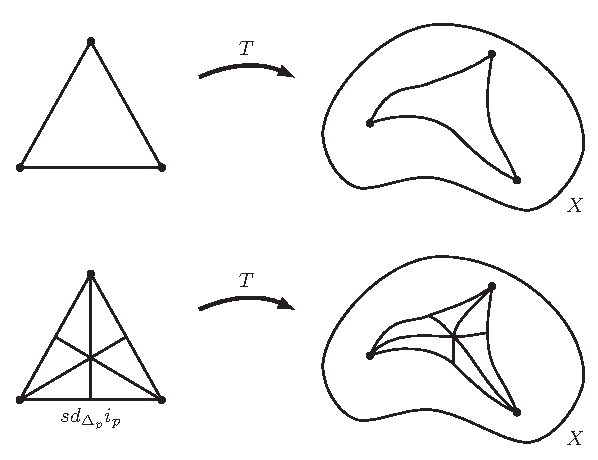
\includegraphics[width=.85\textwidth]{figures/4-4-1.pdf}\\图 4.4.1\end{center}

\entry{引理}{4.4.3}同态 $\operatorname{sd}_X$ 是保持增广的链映射，并具有自然性：对每个连续映射 $f:X\to Y$，有
\[
f_\#\circ\operatorname{sd}_X=\operatorname{sd}_Y\circ f_\#.
\]
\textbf{证明：}因为 $\operatorname{sd}_X$ 在零维为恒等同态，它保持增广，且在零维具有自然性。正维数中的自然性由直接计算得到：
\[
f_\#(\operatorname{sd}_XT)=f_\#T_\#(\operatorname{sd}_{\Delta_p}i_p)
=\operatorname{sd}_Y(f\circ T)=\operatorname{sd}_Y(f_\#T).
\]
以后通常省略下标，由上下文确定 $\operatorname{sd}$ 所指的空间。

\sourcepage{205}
为证明它是链映射，对 $p$ 归纳。零维中 $\operatorname{sd}\partial=\partial\operatorname{sd}$ 显然成立。设在小于 $p$ 的维数已成立。由引理 4.2.8，
\[
\partial\operatorname{sd}i_p=
\begin{cases}
(-1)^p[\partial\operatorname{sd}\partial i_p,\widehat\Delta_p]+\operatorname{sd}\partial i_p,&p>1,\\
-\epsilon(\operatorname{sd}\partial i_1)T_0+\operatorname{sd}\partial i_1,&p=1,
\end{cases}
\]
其中 $T_0$ 的像为 $\widehat\Delta_1$。若 $p>1$，归纳假设给出 $\partial\operatorname{sd}\partial i_p=\operatorname{sd}\partial\partial i_p=0$；若 $p=1$，由保持增广性，$\epsilon(\operatorname{sd}\partial i_1)=\epsilon(\partial i_1)=0$。因此两种情形都有 $\partial\operatorname{sd}i_p=\operatorname{sd}\partial i_p$。一般地，
\begin{align*}
\partial\operatorname{sd}T
&=\partial T_\#(\operatorname{sd}i_p) &&\text{（定义）}\\
&=T_\#(\partial\operatorname{sd}i_p)&&\text{（$T_\#$ 是链映射）}\\
&=T_\#(\operatorname{sd}\partial i_p)&&\text{（刚证明的公式）}\\
&=\operatorname{sd}T_\#(\partial i_p)&&\text{（自然性）}\\
&=\operatorname{sd}\partial(T_\#i_p)=\operatorname{sd}\partial T. &&\text{（$T_\#$ 是链映射）}
\end{align*}
\hfill$\square$

\entry{引理}{4.4.4}若 $T:\Delta_p\to\sigma$ 是到 $p$ 维单形 $\sigma$ 的线性同胚，则 $\operatorname{sd}T$ 的每一项都是从 $\Delta_p$ 到 $\sigma$ 的第一次重心重分中某个单形的线性同胚。

\textbf{证明：}$p=0$ 时显然。设结论在小于 $p$ 的维数成立。先考虑 $i_p:\Delta_p\to\Delta_p$。由定义，
\[
\operatorname{sd}i_p=(-1)^p[\operatorname{sd}\partial i_p,\widehat\Delta_p].
\]
\translatornote{原书在本证明此式中漏印了系数 $(-1)^p$；这不影响关于各项像集的论证。}链 $\partial i_p$ 的每一项都是从 $\Delta_{p-1}$ 到 $\Bd\Delta_p$ 中某个单形的线性同胚。由归纳假设，可写 $\operatorname{sd}\partial i_p=\sum\pm T_i$，其中 $T_i$ 是到 $\Bd\Delta_p$ 的第一次重心重分中某个单形 $\widehat s_1\cdots\widehat s_p$ 的线性同胚。于是 $[T_i,\widehat\Delta_p]$ 是到单形 $\widehat\Delta_p\widehat s_1\cdots\widehat s_p$ 的线性同胚，而该单形属于 $\Delta_p$ 的第一次重心重分。

对于一般的 $T$，由于线性同胚把各面的重心映为相应面的重心，它诱导 $\Delta_p$ 与 $\sigma$ 的第一次重心重分之间的线性同构。由 $\operatorname{sd}T=T_\#(\operatorname{sd}i_p)$，且线性同胚的复合仍为线性同胚，即得结论。\hfill$\square$

\sourcepage{206}
\entry{定理}{4.4.5}设 $\mathcal A$ 是 $X$ 的子集族，其成员的内部覆盖 $X$。给定 $T:\Delta_p\to X$，存在 $m$，使 $\operatorname{sd}^mT$ 的每一项都是 $\mathcal A$-小的。

\textbf{证明：}由上一引理迭代可知：若 $L:\Delta_p\to\sigma$ 为线性同胚，则 $\operatorname{sd}^mL$ 的每一项都是到 $\sigma$ 的第 $m$ 次重心重分中某个单形的线性同胚。

开集 $T^{-1}(\Int A)$（$A\in\mathcal A$）覆盖 $\Delta_p$。取这个开覆盖的 Lebesgue 数 $\lambda$（引理 2.4.1），并取 $m$ 足够大，使 $\Delta_p$ 的第 $m$ 次重心重分中的每个单形直径均小于 $\lambda$。于是 $\operatorname{sd}^mi_p$ 每一项的像集直径均小于 $\lambda$。因此 $\operatorname{sd}^mT=T_\#(\operatorname{sd}^mi_p)$ 中每一项的像都包含于某个 $A\in\mathcal A$。\hfill$\square$

既已说明怎样把奇异链分割为 $\mathcal A$-小的链，下面证明这些链足以生成 $X$ 的同调。先证明一个引理。

\entry{引理}{4.4.6}给定 $m$，对每个空间 $X$ 存在同态 $D_X:S_p(X)\to S_{p+1}(X)$，使对每个奇异单形 $T$ 有
\[
\partial D_XT+D_X\partial T=\operatorname{sd}^mT-T.\tag{*}
\]
而且 $D_X$ 是自然的：若 $f:X\to Y$，则 $f_\#D_X=D_Yf_\#$。

\textbf{证明：}零维中令 $D_XT=0$，则 (*) 及自然性显然成立。设 $p>0$，并设所有空间在小于 $p$ 的维数均已定义满足这些条件的 $D_X$。用与引理 4.3.6 类似的方法；下一节将把它表述为无环模型法。

先取 $X=\Delta_p$、$T=i_p$。令 $c_p=\operatorname{sd}^mi_p-i_p-D_{\Delta_p}(\partial i_p)$。用通常的计算及归纳假设可得 $\partial c_p=0$。因为 $\Delta_p$ 的奇异同调无环，可选取 $D_{\Delta_p}i_p\in S_{p+1}(\Delta_p)$，使其边缘为 $c_p$。于是此特殊情形满足 (*)。

对于任意 $T:\Delta_p\to X$，令 $D_XT=T_\#(D_{\Delta_p}i_p)$。计算得
\begin{align*}
\partial D_XT&=T_\#(\partial D_{\Delta_p}i_p)\\
&=T_\#(\operatorname{sd}^mi_p-i_p-D_{\Delta_p}\partial i_p)\\
&=\operatorname{sd}^mT_\#i_p-T_\#i_p-D_XT_\#\partial i_p\\
&=\operatorname{sd}^mT-T-D_X\partial T.
\end{align*}
倒数第二步使用了 $D_X$ 在 $(p-1)$ 维的自然性。$p$ 维的自然性则直接来自定义。\hfill$\square$

\sourcepage{207}
由 $\operatorname{sd}^m$ 与 $D_X$ 的自然性，若 $A\subset X$，它们分别把 $S_p(A)$ 映入 $S_p(A)$ 与 $S_{p+1}(A)$。故在相对链复形 $\mathcal S(X,A)$ 上，它们也分别诱导链映射与链同伦。

\entry{定义}{4.4.7}设 $\mathcal A$ 覆盖空间 $X$。以 $S_p^{\mathcal A}(X)$ 表示由 $\mathcal A$-小的奇异单形生成的 $S_p(X)$ 的子群，以 $\mathcal S^{\mathcal A}(X)$ 表示由这些链群组成的链复形。它是 $\mathcal S(X)$ 的子链复形：若 $T$ 的像包含于 $A\in\mathcal A$，则 $\partial T$ 每一项的像也包含于 $A$。

每个零维单形自动为 $\mathcal A$-小的，所以 $S_0^{\mathcal A}(X)=S_0(X)$，且 $\epsilon$ 给出其增广。\translatornote{原书此等式左端的下标印为 $p$；应为 $0$。}由上面的观察，$\operatorname{sd}^m$ 和 $D_X$ 都将 $\mathcal S^{\mathcal A}(X)$ 映入自身：若 $T$ 的像包含于 $A\in\mathcal A$，则它们作用后每一项的像仍包含于 $A$。

\entry{定理}{4.4.8}若 $\mathcal A$ 的成员的内部覆盖 $X$，则包含映射 $\mathcal S^{\mathcal A}(X)\to\mathcal S(X)$ 在普通及约化同调中均诱导同构。

\textbf{证明：}一个自然的想法是构造包含映射的链同伦逆 $\lambda:\mathcal S(X)\to\mathcal S^{\mathcal A}(X)$，但这并不容易。对任何特定的链，某个 $\operatorname{sd}^m$ 可以奏效；链变化时，所需的 $m$ 却可能越来越大。我们换一种方法。

考虑短正合列
\[
0\longrightarrow S_p^{\mathcal A}(X)\longrightarrow S_p(X)\longrightarrow S_p(X)/S_p^{\mathcal A}(X)\longrightarrow0.
\]
它给出普通或约化同调的长正合列。因此，只需证明商链复形 $\{S_p(X)/S_p^{\mathcal A}(X),\partial\}$ 在每一维的同调均为零。也就是说，若 $c_p\in S_p(X)$ 满足 $\partial c_p\in S_{p-1}^{\mathcal A}(X)$，只需找到 $d_{p+1}$，使 $c_p+\partial d_{p+1}\in S_p^{\mathcal A}(X)$。

链 $c_p$ 是有限个奇异单形的形式线性组合，由定理 4.4.5，可取统一的 $m$，使 $\operatorname{sd}^mc_p$ 中每个单形均为 $\mathcal A$-小的。取引理 4.4.6 中对应此 $m$ 的 $D_X$，则
\[
c_p+\partial D_Xc_p=\operatorname{sd}^mc_p-D_X\partial c_p.
\]
右端第一项按 $m$ 的选择属于 $S_p^{\mathcal A}(X)$，第二项因 $\partial c_p\in S_{p-1}^{\mathcal A}(X)$ 及前述保持性，也属于此群。取 $d_{p+1}=D_Xc_p$ 即可。\hfill$\square$

\sourcepage{208}
事实上，确实存在包含映射的链同伦逆 $\lambda:\mathcal S(X)\to\mathcal S^{\mathcal A}(X)$。[Vic73] 第 207 页给出了使用 $\operatorname{sd}^m$ 的具体公式。稍后我们还会从更一般的结果导出其存在性，见第 5.7 节习题。\translatornote{原书两处把链同伦逆的方向写成与包含映射相同；上文按其所需的逆向作了修正。}

\entry{推论}{4.4.9}设 $X$、$\mathcal A$ 同上，$B\subset X$。令 $S_p^{\mathcal A}(B)$ 由像包含于 $\mathcal A$ 某个成员的奇异单形 $T:\Delta_p\to B$ 生成，且令 $S_p^{\mathcal A}(X,B)=S_p^{\mathcal A}(X)/S_p^{\mathcal A}(B)$。则包含映射 $S_p^{\mathcal A}(X,B)\to S_p(X,B)$ 诱导同调同构。

\textbf{证明：}包含映射给出由两条短正合列
\begin{gather*}
0\longrightarrow\mathcal S^{\mathcal A}(B)\longrightarrow\mathcal S^{\mathcal A}(X)\longrightarrow\mathcal S^{\mathcal A}(X,B)\longrightarrow0,\\
0\longrightarrow\mathcal S(B)\longrightarrow\mathcal S(X)\longrightarrow\mathcal S(X,B)\longrightarrow0
\end{gather*}
导出的长正合列之间的同态。绝对同调上的同态由上一定理为同构，再由 Steenrod 五引理（引理 3.3.4），相对同调上的同态也为同构。\hfill$\square$

\entry{定理}{4.4.10（奇异同调的切除定理）}设 $A\subset X$。若 $U\subset X$ 满足 $\overline U\subset\Int A$，则包含映射
\[
j:(X\setminus U,A\setminus U)\to(X,A)
\]
在奇异同调中诱导同构。

\textbf{证明：}取 $\mathcal A=\{X\setminus U,A\}$。因为 $X\setminus\overline U\subset\Int(X\setminus U)$，且 $\overline U\subset\Int A$，这些集合的内部覆盖 $X$。考虑包含映射诱导的同态
\[
\frac{S_p(X\setminus U)}{S_p(A\setminus U)}\longrightarrow
\frac{S_p^{\mathcal A}(X)}{S_p^{\mathcal A}(A)}\longrightarrow
\frac{S_p(X)}{S_p(A)}.
\]
由上一推论，第二个同态诱导同调同构。下面证明第一个在链的层次上就已是同构。

\sourcepage{209}
包含映射诱导 $\varphi:S_p(X\setminus U)\to S_p^{\mathcal A}(X)/S_p^{\mathcal A}(A)$。若 $c_p\in S_p^{\mathcal A}(X)$，其每一项的像或包含于 $X\setminus U$，或包含于 $A$。形成模 $S_p^{\mathcal A}(A)$ 的陪集时，可删去后面这些项，所以 $\varphi$ 满射。而
\[
\ker\varphi=S_p(X\setminus U)\cap S_p^{\mathcal A}(A)
=S_p((X\setminus U)\cap A)=S_p(A\setminus U).
\]
故第一个同态为同构，证明完成。\hfill$\square$

这个定理比切除公理本身（第 3.5 节）略强：奇异同调论中不必假设 $U$ 是 $X$ 的开子集。作为应用，计算球和球面的奇异同调。

\entry{定理}{4.4.11}设 $n\ge0$。群 $H_i(B^n,S^{n-1})$ 在 $i=n$ 时为无限循环群，其余情形为零。群 $\widetilde H_i(S^n)$ 也在 $i=n$ 时为无限循环群，其余情形为零。反射映射
\[
\rho_1(x_1,x_2,\ldots,x_{n+1})=(-x_1,x_2,\ldots,x_{n+1})
\]
在 $\widetilde H_n(S^n)$ 上诱导的同态是乘以 $-1$。

\entry{注}{4.4.12}回忆定义 2.9.1，$n\ge1$ 时，这说明反射映射的度为 $-1$。

\textbf{定理的证明：}先设 $n=0$。空间 $B^0$ 为单点空间，$S^{-1}=\varnothing$，因为单位球面上的点必须有范数 $1$。由定理 4.3.3，$H_p(B^0,\varnothing)$ 在 $p=0$ 时为无限循环群，其余为零。

将定理 4.3.3 的证明推广到双点空间 $S^0=\{-1,+1\}$，可得 $p>0$ 时 $H_p(S^0)=0$，且 $H_0(S^0)=\Z\oplus\Z$，基为 $T_{-1}$、$T_{+1}$。所以 $\widetilde H_0(S^0)$ 为无限循环群，生成元为 $T_{+1}-T_{-1}$。映射 $\rho_1$ 交换两个点，故诱导同态为乘以 $-1$。

现作归纳。设定理在 $n-1$ 维成立，$n\ge1$。因 $B^n$ 可缩，$(B^n,S^{n-1})$ 的长正合列给出
\[
H_i(B^n,S^{n-1})\cong\widetilde H_{i-1}(S^{n-1}).
\]
所以左端在 $i=n$ 时为无限循环群，其余为零。

\sourcepage{210}
\begin{center}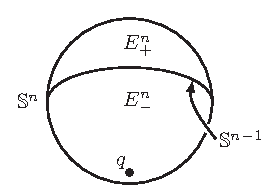
\includegraphics[width=.45\textwidth]{figures/4-4-2.pdf}\\图 4.4.2\end{center}
为计算 $\widetilde H_i(S^n)$，考虑同态图
\[
\begin{array}{ccc}
H_i(E^n_+,S^{n-1})&\xrightarrow{\partial_*}&\widetilde H_{i-1}(S^{n-1})\\
\downarrow\scriptstyle k_*&&\\
H_i(S^n\setminus\{q\},E^n_-\setminus\{q\})&&\\
\downarrow\scriptstyle j_*&&\\
H_i(S^n,E^n_-)&\xleftarrow{\ i_*\ }&\widetilde H_i(S^n),
\end{array}
\]
其中 $i,j,k$ 均为包含映射，$q=(0,\ldots,0,-1)$ 为南极。我们将证明四个同态 $i_*,j_*,k_*,\partial_*$ 都是同构，从而得到 $\widetilde H_i(S^n)\cong\widetilde H_{i-1}(S^{n-1})$。

回忆 $E^n_+$、$E^n_-$ 分别为上下半球，而 $S^{n-1}=E^n_+\cap E^n_-$ 是赤道。两个半球都是 $n$ 维球：$\R^{n+1}$ 到 $\R^n\times\{0\}$ 的投影把每个半球同胚地映到 $B^n$，也把 $E^n_-\setminus\{q\}$ 同胚地映到 $B^n\setminus\{0\}$。

特别地，$E^n_-$ 可缩，故 $(S^n,E^n_-)$ 的长正合列说明 $i_*$ 为同构。因 $q\in\Int E^n_-$，切除定理说明 $j_*$ 为同构。又因 $S^{n-1}$ 是 $E^n_-\setminus\{q\}$ 的形变收缩核，而 $E^n_+$ 是 $S^n\setminus\{q\}$ 的形变收缩核，$k_*$ 也是同构。〔空间偶 $(E^n_-\setminus\{q\},S^{n-1})$ 同胚于 $(B^n\setminus\{0\},S^{n-1})$，因而有到赤道的形变收缩 $F_t$；在 $E^n_+$ 上令每个 $F_t$ 为恒等映射，就将它延拓为 $S^n\setminus\{q\}$ 到 $E^n_+$ 的形变收缩。〕最后，$E^n_+$ 可缩，故 $\partial_*$ 为同构。归纳假设遂给出球面同调的结论。

反射 $\rho_1$ 将 $q$、上下半球及球面分别映入自身，故诱导上图到自身的同态。按归纳假设，它在 $\widetilde H_{n-1}(S^{n-1})$ 上为乘以 $-1$；由图中各同构及自然性，在 $\widetilde H_n(S^n)$ 上也如此。\hfill$\square$

\sourcepage{211}
注意上述证明中，真正直接计算的只有单点空间和双点空间的同调群。

\entry{推论}{4.4.13}若 $a:S^n\to S^n$ 是对径映射 $a(x)=-x$，则 $a_*$ 是乘以 $(-1)^{n+1}$。

\subsection*{习题}
\begin{enumerate}
\item 把引理 4.4.3、4.4.6 的自然性表述为 $\operatorname{sd}$、$D_X$ 是某些函子之间的自然变换。
\item 设 $X=\{(x,y):1<x^2+y^2<4\}\subset\R^2$ 为圆环，$\mathcal A$ 是平面内所有开圆盘组成的族。给出一个 $X$ 中 $\mathcal A$-小的奇异单形。
\item 对 $\R^3$ 中的单位球面 $X$，以及所有棱平行于坐标轴的开立方体组成的族 $\mathcal A$，重复习题 2。
\end{enumerate}

\section{\texorpdfstring{*无环模型}{*无环模型}}
\sourcepage{211}
本节假定读者熟悉第 3.7 节“范畴与函子”。这里的结果将在第 7.9 节证明 Eilenberg--Zilber 定理时使用。

前两节构造了某些自然链同伦 $D_X$。方法是先在特殊空间 $\Delta_p$ 的特殊奇异单形 $i_p$ 上定义它。为此，需要另一个空间的无环性：第 4.3 节中是 $\Delta_p\times I$，第 4.4 节中则是 $\Delta_p$。这一步涉及任意选择，此后的构造却都由自然性所迫定。这与早先使用无环载体的构造十分相似，但也有区别。

现在把这种方法形式化，以备以后使用。我们将陈述一个足以满足需要的定理，称为无环模型定理。其表述相当抽象，可能令某些读者感到困难。为便于理解，先简要回顾所用的范畴论术语。

\sourcepage{212}
本节始终以 $\mathcal C$ 表示任意范畴，对象记为 $X,Y,\ldots$，态射记为 $f,g,\ldots$；以 $\mathcal A$ 表示增广链复形及其链映射组成的范畴。大多数应用中，$\mathcal C$ 是拓扑范畴，或以有序的两个拓扑空间为对象、以成对连续映射为态射的范畴。读者愿意的话，只考虑这些范畴即可。

我们讨论从 $\mathcal C$ 到 $\mathcal A$ 的函子 $G,G'$（定义 3.7.3）。它们把对象 $X$ 分别映为增广链复形 $G(X),G'(X)$，其 $p$ 维链群为 $G_p(X),G'_p(X)$。另一个对象 $Y$ 同样给出两套链群。对于态射 $f\in\operatorname{hom}(X,Y)$，函子给出增广链复形的链映射
\[
G(f):G(X)\to G(Y),\qquad G'(f):G'(X)\to G'(Y).
\]
这里链映射的含义见定义 1.14.2。

从 $G$ 到 $G'$ 的自然变换 $T$（定义 3.7.6）给每个对象 $X$ 指定一个增广链复形的链映射 $T_X:G(X)\to G'(X)$，并要求对每个 $f:X\to Y$，下图交换：
\[
\begin{array}{ccc}
G_p(X)&\xrightarrow{T_X}&G'_p(X)\\
\downarrow\scriptstyle G(f)&&\downarrow\scriptstyle G'(f)\\
G_p(Y)&\xrightarrow{T_Y}&G'_p(Y).
\end{array}
\]
对于两个自然变换 $S,T:G\to G'$，还可考虑它们之间的\textbf{自然链同伦}（natural chain homotopy）$D$。它给每个 $X$ 指定一族同态 $D_X:G_p(X)\to G'_{p+1}(X)$，满足
\[
\partial'D_X+D_X\partial=T_X-S_X,
\]
且对每个 $f:X\to Y$，下图交换：
\[
\begin{array}{ccc}
G_p(X)&\xrightarrow{D_X}&G'_{p+1}(X)\\
\downarrow\scriptstyle G(f)&&\downarrow\scriptstyle G'(f)\\
G_p(Y)&\xrightarrow{D_Y}&G'_{p+1}(Y).
\end{array}
\]

\sourcepage{213}
\entry{定义}{4.5.1}设 $G,G':\mathcal C\to\mathcal A$ 为函子，$\mathcal M$ 是 $\mathcal C$ 中一族对象，称为\textbf{模型}或\textbf{模型对象}（models, model objects）。
\begin{enumerate}[label=(\arabic*)]
\item 若每个 $M\in\mathcal M$ 都使 $G'(M)$ 无环，则称 $G'$ \textbf{相对于 $\mathcal M$ 无环}。
\item 若对每个 $p\ge0$，存在指标集 $J_p$、模型对象族 $\{M_\alpha\}_{\alpha\in J_p}$ 以及元素族 $i_\alpha\in G_p(M_\alpha)$，满足下述条件，则称 $G$ \textbf{相对于 $\mathcal M$ 自由}：对于每个 $X$，当 $\alpha$ 遍历 $J_p$、$f$ 遍历 $\operatorname{hom}(M_\alpha,X)$ 时，诸元素 $G(f)(i_\alpha)\in G_p(X)$ 彼此不同，并构成 $G_p(X)$ 的一组基。
\end{enumerate}
因此，自由函子所给出的每个 $G_p(X)$ 都是自由阿贝尔群。我们将先在基元上构造映射；要求这些基元彼此不同，是为了避免不同构造给同一个基元指定不相等的像。

\entry{例}{4.5.2}考虑拓扑范畴到 $\mathcal A$ 的奇异链复形函子。取 $\mathcal M=\{\Delta_p:p=0,1,\ldots\}$，它相对于 $\mathcal M$ 无环。它也相对自由：对每个 $p$，令 $J_p$ 只有一个元素，相应模型为 $\Delta_p$，相应基元为恒等奇异单形 $i_p\in S_p(\Delta_p)$。当 $T$ 遍历所有连续映射 $\Delta_p\to X$ 时，$T_\#i_p=T$ 恰遍历 $S_p(X)$ 的一组基。

\entry{例}{4.5.3}考虑定义在成对拓扑空间范畴上的函子
\[
G(X,Y)=\mathcal S(X\times Y),\qquad G(f,g)=(f\times g)_\#.
\]
令 $\mathcal M=\{(\Delta_p,\Delta_q):p,q\ge0\}$。因为 $\Delta_p\times\Delta_q$ 可缩，$G$ 相对于 $\mathcal M$ 无环。为证明相对自由，对每个 $p$ 令 $J_p$ 只有一个元素，模型为 $(\Delta_p,\Delta_p)$，相应奇异单形为对角映射 $d_p(x)=(x,x)$。当 $f:\Delta_p\to X$、$g:\Delta_p\to Y$ 遍历所有连续映射时，$(f\times g)_\#d_p$ 恰遍历所有 $\Delta_p\to X\times Y$ 的连续映射，且表示唯一，故构成一组基。

\sourcepage{214}
\entry{例}{4.5.4}设 $G(X)=\mathcal S(X\times I)$，$G(f)=(f\times i_I)_\#$。对于 $\mathcal M=\{\Delta_p:p\ge0\}$，$G$ 相对无环。它也相对自由，但证明稍复杂。令 $J_p$ 为所有连续函数 $\alpha:\Delta_p\to I$ 构成的集合；对每个 $\alpha$，令 $M_\alpha=\Delta_p$，并取
\[
i_\alpha:\Delta_p\to\Delta_p\times I,\qquad i_\alpha(x)=(x,\alpha(x)).
\]
当 $f$ 遍历所有 $\Delta_p\to X$ 的连续映射、$\alpha$ 遍历 $J_p$ 时，$(f\times i_I)_\#i_\alpha$ 恰遍历 $S_p(X\times I)$ 的一组基。

若 $G$ 相对于 $\mathcal M$ 自由，它也相对于任何更大的模型族自由；若它相对于 $\mathcal M$ 无环，它也相对于任何更小的模型族无环。因此，要同时满足两者，模型族的大小必须选得适当。

\entry{定理}{4.5.5（无环模型定理）}设 $G,G'$ 是从范畴 $\mathcal C$ 到增广链复形及其链映射范畴 $\mathcal A$ 的函子，$\mathcal M$ 是一族模型对象。若 $G$ 相对于 $\mathcal M$ 自由，$G'$ 相对于 $\mathcal M$ 无环，则：
\begin{enumerate}[label=(\alph*)]
\item 存在自然变换 $T:G\to G'$。
\item 对任意两个自然变换 $S,T:G\to G'$，存在它们之间的自然链同伦 $D$。
\end{enumerate}
习题 1、2 给出了证明步骤。若习题 1 太困难，可以先做习题 2，并参考引理 4.3.6 的证明及其后关于零维情形的说明；理解习题 2 后再返回习题 1。

无环模型法最先由 Eilenberg 与 MacLane 在 [EM53] 中形式化。在同一期《美国数学杂志》紧接着的一篇论文 [EZ53] 中，Eilenberg 与 Zilber 应用了这一方法。

\entry{推论}{4.5.6}若 $G,G':\mathcal C\to\mathcal A$ 都相对于 $\mathcal M$ 自由且无环，则存在自然变换 $T:G\to G'$；任何这样的变换都是自然链同伦等价。\translatornote{原书称为“自然等价”；本证明所给出的是链同伦意义下的等价，并非各链群上都有严格逆的自然同构。}

\sourcepage{215}
\textbf{证明：}四次应用上一定理。由 $G$ 自由、$G'$ 无环，得 $T$；由 $G'$ 自由、$G$ 无环，得 $S:G'\to G$。于是 $S\circ T$ 与恒等变换是从 $G$ 到自身的两个自然变换。因 $G$ 自由且无环，它们之间有自然链同伦。同理由 $G'$ 自由且无环，$T\circ S$ 也自然链同伦于恒等变换。\hfill$\square$

\subsection*{习题}
\begin{enumerate}
\item 按下列步骤证明无环模型定理的 (a)。
\begin{enumerate}[label=(\alph*)]
\item 固定 $M_\alpha\in\mathcal M$、$c\in G_p(M_\alpha)$，$p\ge0$。证明可选链 $d'\in G'_p(M_\alpha)$，令 $T_{M_\alpha}(c)=d'$，使
\[
\epsilon'T_{M_\alpha}(c)=\epsilon(c)\ (p=0),\qquad
\partial'T_{M_\alpha}(c)=T_{M_\alpha}\partial c\ (p>0).
\]
其中 $\epsilon',\partial'$ 是 $G'$ 的增广和边缘，$\epsilon,\partial$ 是 $G$ 的增广和边缘。〔提示：对 $p$ 归纳。〕\translatornote{原书将 $d'$ 所在群漏印为 $G_p(M_\alpha)$；应为 $G'_p(M_\alpha)$。}
\item (a) 中只在模型对象上构造了 $T$。由自由性，公式
\[
T_XG(f)(i_\alpha)=G'(f)T_{M_\alpha}(i_\alpha),\qquad
\alpha\in J_p,\ f\in\operatorname{hom}(M_\alpha,X),
\]
把它延拓到所有 $X\in\mathcal C$。证明这个变换自然。
\item 证明 (b) 所定义的变换满足 $\epsilon'T_X=\epsilon$（$p=0$），以及 $\partial'T_X=T_X\partial$（$p>0$）。
\end{enumerate}
\item 按下列步骤证明无环模型定理的 (b)。
\begin{enumerate}[label=(\alph*)]
\item 固定 $M_\alpha\in\mathcal M$、$c\in G_p(M_\alpha)$。证明可选 $d'\in G'_{p+1}(M_\alpha)$，令 $D_{M_\alpha}(c)=d'$，使
\begin{gather*}
\partial'D_{M_\alpha}(c)=(T_{M_\alpha}-S_{M_\alpha})(c),\qquad p=0,\\
\partial'D_{M_\alpha}(c)+D_{M_\alpha}(\partial c)=(T_{M_\alpha}-S_{M_\alpha})(c),\qquad p>0.
\end{gather*}
〔提示：对 $p$ 归纳。〕\translatornote{原书同样在 $d'$ 所在群漏印了撇号。}
\item 由 $G$ 的自由性，用公式
\[
D_XG(f)(i_\alpha)=G'(f)D_{M_\alpha}(i_\alpha),\qquad
\alpha\in J_p,\ f\in\operatorname{hom}(M_\alpha,X),
\]
把模型上的链同伦延拓到所有对象。证明它自然。
\item[(d)] 证明上述变换满足
\[
\partial'D_X=T_X-S_X\ (p=0),\qquad
\partial'D_X+D_X\partial=T_X-S_X\ (p>0),
\]
因此是 $S,T$ 之间的自然链同伦。\translatornote{保留原书跳过 (c) 的题号。原书零维公式右端误作 $T_X-S_{M_\alpha}$，已按定义改为 $T_X-S_X$。}
\end{enumerate}
\sourcepage{216--217}
\item 考虑拓扑范畴到 $\mathcal A$ 的函子 $G(X)=\mathcal S(X)$、$G(f)=f_\#$，以及 $G'(X)=\mathcal S(X\times I)$、$G'(f)=(f\times i_I)_\#$。
\begin{enumerate}[label=(\alph*)]
\item 令 $i(x)=(x,0)$、$j(x)=(x,1)$。证明 $T_X(T)=i_\#T$、$T'_X(T)=j_\#T$ 定义自然变换，并由无环模型定理推出引理 4.3.6。
\item 证明 $\operatorname{sd}^m$ 与 $(i_X)_\#$ 是 $G$ 到自身的自然变换，从而由无环模型定理推出引理 4.4.6。
\end{enumerate}
\item 设 $K,L$ 是单纯复形，$\Phi$ 是从 $K$ 到 $L$ 的无环载体。以 $K$ 的子复形为对象、包含映射为态射组成范畴 $\mathcal C$。对于子复形 $K_0$，令 $\Phi(K_0)$ 为所有 $\Phi(\sigma)$（$\sigma$ 遍历 $K_0$ 的单形）之并。
\begin{enumerate}[label=(\alph*)]
\item 对包含映射 $j:K_0\to K_1$，考虑 $G(K_0)=\mathcal C(K_0)$、$G(j)=j_\#$，以及 $G'(K_0)=\mathcal C(\Phi(K_0))$、$G'(j)=\ell_\#$，其中 $\ell:\Phi(K_0)\to\Phi(K_1)$ 是包含映射。证明这确实定义了函子。
\item 由无环模型定理推出定理 1.14.10，即几何形式的无环载体定理。〔提示：取 $\mathcal M$ 为所有其多面体是 $K$ 中某个单形的子复形。〕
\end{enumerate}
\item 给出一个无环函子的例子。
\item 给出一个自由函子的例子。
\end{enumerate}

\section{Mayer--Vietoris 序列}
\sourcepage{217}
若 $X=X_1\cup X_2$，在适当条件下，存在把 $X$ 的同调与 $X_1,X_2$ 的同调联系起来的正合列，称为这两个子空间的 \textbf{Mayer--Vietoris 序列}。单纯同调中，我们在 $X_1,X_2$ 是某个复形的子复形的多面体时构造过它。奇异同调需要类似的条件。

\entry{定义}{4.6.1}设 $X=X_1\cup X_2$，令 $\mathcal U=\{X_1,X_2\}$，记
\[
\mathcal S(X_1)+\mathcal S(X_2)=\mathcal S^{\mathcal U}(X).
\]
其 $p$ 维链群是 $S_p(X_1)+S_p(X_2)$；除非两个子空间不交，否则这不是直和。若包含映射
\[
\mathcal S(X_1)+\mathcal S(X_2)\longrightarrow\mathcal S(X)
\]
诱导同调同构，则称 $\{X_1,X_2\}$ 为\textbf{可切除对}（excisive couple）。

对于奇异同调，这一定义等价于第 3.5 节习题 3 中的定义，证明留作习题 2。由定理 4.4.8，若 $\Int X_1$ 与 $\Int X_2$ 覆盖 $X$，则它们构成可切除对。

\entry{定理}{4.6.2}设 $X=X_1\cup X_2$，$\{X_1,X_2\}$ 为可切除对，$A=X_1\cap X_2$。则有正合列
\[
\begin{split}
\cdots\longrightarrow H_p(A)\xrightarrow{\varphi_*}H_p(X_1)\oplus H_p(X_2)
\xrightarrow{\psi_*}H_p(X)\\
\xrightarrow{\partial_*}H_{p-1}(A)\longrightarrow\cdots,
\end{split}
\]
称为 $\{X_1,X_2\}$ 的 Mayer--Vietoris 序列。\translatornote{原书显示的序列漏印了 $H_p(X)$ 及其后的连接同态。}其中
\[
\varphi_*(a)=(i_*a,-j_*a),\qquad \psi_*(x_1,x_2)=k_*x_1+\ell_*x_2,
\]
而 $i:A\to X_1$、$j:A\to X_2$、$k:X_1\to X$、$\ell:X_2\to X$ 都是包含映射。若 $A\ne\varnothing$，约化同调也有类似序列。两种序列对连续映射诱导的同态都具有自然性。

\sourcepage{218}
\textbf{证明：}定义链复形的短正合列
\[
0\longrightarrow S_p(A)\xrightarrow{\varphi}S_p(X_1)\oplus S_p(X_2)
\xrightarrow{\psi}S_p(X_1)+S_p(X_2)\longrightarrow0,\tag{*}
\]
其中 $\varphi(c)=(i_\#c,-j_\#c)$，$\psi(c_1,c_2)=k_\#c_1+\ell_\#c_2$。映射 $\varphi$ 单射，$\psi$ 满射；其核由所有 $(c,-c)$ 组成，其中 $c$ 同时属于 $S_p(X_1)$、$S_p(X_2)$，即属于 $S_p(A)$。故序列正合。

之字形引理（引理 3.3.2）给出长正合列，而可切除性保证
\[
H_p(\mathcal S(X_1)+\mathcal S(X_2))\cong H_p(X).\tag{**}
\]
所以得到所需序列。若 $A\ne\varnothing$，同样论证可用于约化同调。

若 $f:(X,X_1,X_2)\to(Y,Y_1,Y_2)$ 连续，且两边均为可切除对，则 $f_\#$ 与包含映射可交换，因而与 $\varphi,\psi$ 可交换，给出短正合列间的同态，进而给出长正合列间的同态。同构 (**) 由包含映射诱导，也与 $f_*$ 可交换。这就证明了自然性。\hfill$\square$

下面给出 Mayer--Vietoris 序列的一个应用。回忆：若 $w_0*K$、$w_1*K$ 是两个锥，其多面体仅在 $|K|$ 相交，则并为 $K$ 的悬挂 $S(K)$（第 3.4 节）。映射
\[
\pi:|K|\times[-1,1]\to|S(K)|,\qquad
\pi(x,t)=\begin{cases}(1-t)x+tw_0,&t\ge0,\\(1+t)x-tw_1,&t\le0,\end{cases}
\]
是商映射，把 $|K|\times\{1\}$ 压缩为 $w_0$、把 $|K|\times\{-1\}$ 压缩为 $w_1$，在其余部分一一对应。\translatornote{原书第二行末项为 $+tw_1$；应为 $-tw_1$，使 $t=-1$ 时的像为 $w_1$。}证明与锥的相应结论类似（推论 2.8.8）。由此引出一般拓扑空间的悬挂。

\sourcepage{219}
\entry{定义}{4.6.3}空间 $X$ 的\textbf{悬挂}（suspension）是将 $X\times[-1,1]$ 中的 $X\times\{1\}$ 压缩为一点 $v$、将 $X\times\{-1\}$ 压缩为另一点 $w$ 所得的商空间，记为 $S(X)$。点 $v,w$ 称为\textbf{悬挂点}。

如同单纯同调的情形，可以用 Mayer--Vietoris 序列计算悬挂的同调。

\entry{定理}{4.6.4}对每个 $p$，存在同构 $\widetilde H_p(S(X))\to\widetilde H_{p-1}(X)$。

\textbf{证明：}令 $\pi:X\times[-1,1]\to S(X)$ 为商映射，$v,w$ 为两个悬挂点。取 $X_1=S(X)\setminus\{w\}$、$X_2=S(X)\setminus\{v\}$。它们都是开集，故为可切除对。下面证明两者无环，于是 Mayer--Vietoris 序列给出
\[
\widetilde H_p(S(X))\cong\widetilde H_{p-1}(X_1\cap X_2).
\]
还将证明 $X_1\cap X_2$ 同伦等价于 $X$，从而 $\widetilde H_{p-1}(X_1\cap X_2)\cong\widetilde H_{p-1}(X)$，即得结论。\translatornote{原书后一同构左端误印为 $\widetilde H_p(X_1\cap X_2)$；同伦等价诱导的是同维同调之间的同构。}

集合 $X\times(-1,1]$ 在 $X\times[-1,1]$ 中开，且关于 $\pi$ 饱和，故限制映射 $\pi':X\times(-1,1]\to X_1$ 是商映射。定义
\[
F:X\times(-1,1]\times I\to X\times(-1,1],\qquad
F(x,s,t)=(x,(1-t)s+t).
\]
它给出到 $X\times\{1\}$ 的形变收缩。复合 $\pi'\circ F$ 在 $\pi'\times i_I$ 的每个纤维上为常值，故诱导连续映射 $G:X_1\times I\to X_1$，使下图交换：
\[
\begin{array}{ccc}
X\times(-1,1]\times I&\xrightarrow{F}&X\times(-1,1]\\
\downarrow\scriptstyle\pi'\times i_I&&\downarrow\scriptstyle\pi'\\
X_1\times I&\xrightarrow{G}&X_1.
\end{array}
\]
\sourcepage{220}
这里由定理 2.8.2，$\pi'\times i_I$ 仍是商映射。映射 $G$ 给出 $X_1$ 到 $v$ 的形变收缩，所以 $X_1$ 无环。同理 $X_2$ 无环。

最后，限制映射 $\pi'':X\times(-1,1)\to X_1\cap X_2$ 是一一对应的商映射，故为同胚。而 $X\times\{0\}$ 是 $X\times(-1,1)$ 的形变收缩核，所以 $X$ 与 $X_1\cap X_2$ 同伦等价。\hfill$\square$

\entry{定义}{4.6.5}图 4.6.1 为\textbf{闭合的拓扑学家正弦曲线}（closed topologist's sine curve）。它是定义 4.2.11 中的正弦曲线与一条弧之并；该弧与原曲线仅在 $(0,-1)$、$(1,\sin1)$ 两点相交。习题 1 将用到它。
\begin{center}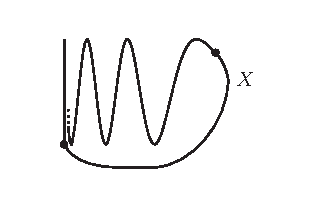
\includegraphics[width=.52\textwidth]{figures/4-6-1.pdf}\\图 4.6.1：闭合的拓扑学家正弦曲线\end{center}

\subsection*{习题}
\begin{enumerate}
\item 选取适当的 Mayer--Vietoris 序列，计算闭合的拓扑学家正弦曲线 $X$ 的奇异同调。
\item 证明：$\{X_1,X_2\}$ 为奇异同调中的可切除对，当且仅当包含映射 $(X_1,X_1\cap X_2)\to(X,X_2)$ 诱导奇异同调同构。〔提示：构造正合列
\[
0\to\mathcal S(X_2)\to\mathcal S(X_1)+\mathcal S(X_2)\to
\mathcal S(X_1)/\mathcal S(X_1\cap X_2)\to0,
\]
并把其导出的长正合列与 $\mathcal S(X,X_2)$ 的同调序列比较。〕
\item 证明 $n\ge1$ 时 $S^n$ 同胚于 $S(S^{n-1})$。利用这一事实计算 $S^n$ 的奇异同调。
\item 陈述并证明相对 Mayer--Vietoris 序列，其中中间的群为 $H_p(X_1,B_1)\oplus H_p(X_2,B_2)$，并假定 $\{X_1,X_2\}$、$\{B_1,B_2\}$ 均可切除。〔提示：把
\[
0\to\mathcal S(B_1\cap B_2)\to\mathcal S(B_1)\oplus\mathcal S(B_2)\to\mathcal S(B_1)+\mathcal S(B_2)\to0
\]
作为定理 4.6.2 证明中序列 (*) 的子序列，应用第 3.3 节习题 2 的蛇引理。〕
\item 设 $X=X_1\cup X_2$、$A=X_1\cap X_2$。假定 $X_1,X_2$ 在 $X$ 中闭，且 $A$ 是 $X_2$ 中某个开集 $U$ 的形变收缩核。证明 $X_1$ 是 $U\cup X_1$ 的形变收缩核，并证明 $\{X_1,X_2\}$ 可切除。
\item 设 $X_1$ 是闭上半圆，$X_2$ 是闭下半圆，$X$ 是平面中的完整单位圆。在这种情形，Mayer--Vietoris 序列给出什么结论？
\item 设 $X_1$ 是闭上半球面，$X_2$ 是闭下半球面，$X$ 是三维空间中的完整单位球面。在这种情形，Mayer--Vietoris 序列给出什么结论？
\end{enumerate}

\section{单纯同调与奇异同调之间的同构}
\sourcepage{221--222}
本节证明：若 $K$ 是单纯复形，则 $K$ 的单纯同调群同构于 $|K|$ 的奇异同调群。这个同构还与诱导同态及边缘同态 $\partial_*$ 可交换，所以它是两种同调理论之间的同构。

证明使用第 1.14 节的有序链复形 $\{C'_p(K),\partial'\}$。那里已证明，有序同调群同构于通常的有向单纯同调群。本节再证明它同构于 $|K|$ 的奇异同调群，从而在多面体上把单纯同调与奇异同调联系起来。

回忆有序 $p$ 维单形是顶点的 $(p+1)$ 元组 $(v_0,\ldots,v_p)$，其中顶点可重复，但必须张成 $K$ 中的一个单形。群 $C'_p(K)$ 以这些元组为自由基，且
\[
\partial'(v_0,\ldots,v_p)=\sum_{i=0}^p(-1)^i(v_0,\ldots,\widehat v_i,\ldots,v_p),\qquad \epsilon'(v)=1.
\]

\entry{定义}{4.7.1}定义 $\theta:C'_p(K)\to S_p(|K|)$，令
\[
\theta((v_0,\ldots,v_p))=\ell(v_0,\ldots,v_p).
\]
即把有序单形映为将 $\epsilon_i$ 映到 $v_i$ 的线性奇异单形。由定义，$\theta$ 是保持增广的链映射，并与包含映射可交换。因此对任何子复形 $K_0$，它诱导相对链映射
\[
\theta:C'_p(K,K_0)\to S_p(|K|,|K_0|).
\]
为证明 $\theta_*$ 是同构，先给出一个引理。

\entry{引理}{4.7.2}设 $\psi:C\to C'$ 是增广链复形的链映射。则 $\psi_*$ 在约化同调上为同构，当且仅当它在普通同调上为同构。

\textbf{证明：}回忆 $H_0(C)\cong\widetilde H_0(C)\oplus\Z$ 的证明（第 1.8 节习题）。考虑交换图
\[
\begin{array}{ccccccccc}
0&\to&\ker\epsilon&\to&C_0&\xrightarrow{\epsilon}&\Z&\to&0\\
&&\downarrow\scriptstyle\psi&&\downarrow\scriptstyle\psi&&\downarrow\scriptstyle=&&\\
0&\to&\ker\epsilon'&\to&C'_0&\xrightarrow{\epsilon'}&\Z&\to&0.
\end{array}
\]
取 $j:\Z\to C_0$，使 $\epsilon\circ j=\operatorname{id}_{\Z}$，并令 $j'=\psi j$。\translatornote{原书把分裂条件写为 $j\circ\epsilon$ 是恒等映射；正确的条件为 $\epsilon\circ j=\operatorname{id}_{\Z}$。}两个短正合列分别由 $j,j'$ 分裂，故
\[
C_0=\ker\epsilon\oplus\operatorname{im}j,\qquad C'_0=\ker\epsilon'\oplus\operatorname{im}j'.
\]
映射 $\psi$ 把 $\operatorname{im}j$ 同构地映到 $\operatorname{im}j'$，而
\[
H_0(C)\cong\frac{\ker\epsilon}{\partial C_1}\oplus\operatorname{im}j,\qquad
H_0(C')\cong\frac{\ker\epsilon'}{\partial'C'_1}\oplus\operatorname{im}j'.
\]
因此普通零维同调上的同态为同构，恰当且仅当约化零维同调上的同态为同构。正维数中两种同调本来相同。\hfill$\square$

\entry{引理}{4.7.3}若 $K_0$ 是 $K$ 的子复形，则对每个 $p$，$\theta$ 诱导同构
\begin{enumerate}[label=(\arabic*)]
\item $\theta_*:\widetilde H_p(\mathcal C'(K))\to\widetilde H_p(|K|)$；
\item $\theta_*:H_p(\mathcal C'(K))\to H_p(|K|)$；
\item $\theta_*:H_p(\mathcal C'(K,K_0))\to H_p(|K|,|K_0|)$。
\end{enumerate}

\sourcepage{223}
\textbf{证明：}可设 $K_0\ne K$，否则 (3) 显然。

\textbf{步骤 1：}先对有限复形按单形个数 $n$ 归纳。若 $n=1$，$K$ 只有一个顶点 $v$。每一维只有一个有序单形 $(v,\ldots,v)$，也只有一个奇异单形 $T:\Delta_p\to\{v\}$，且 $\theta(v,\ldots,v)=T$。所以 $\theta$ 在链的层次上就是同构，三个结论都成立。

设对少于 $n$ 个单形的复形结论成立，而 $K$ 有 $n$ 个单形。只需证明 (1)：由引理 4.7.2 可得 (2)；对子复形 $K_0$ 应用归纳假设，再由长正合列及 Steenrod 五引理可得 (3)。

取 $K$ 中维数最大的单形 $\sigma$。它不是其他单形的真面，故删去 $\sigma$ 后其余单形组成有 $n-1$ 个单形的子复形 $K_1$。令 $\Sigma$ 由 $\sigma$ 及其所有面组成，$\Bd\Sigma$ 由其真面组成。考虑交换图
\[
\begin{array}{ccc}
\widetilde H_p(\mathcal C'(K))&\xrightarrow{\theta_*}&\widetilde H_p(|K|)\\
\downarrow\scriptstyle i_*&&\downarrow\scriptstyle i_*\\
H_p(\mathcal C'(K,\Sigma))&\xrightarrow{\theta_*}&H_p(|K|,\sigma)\\
\uparrow\scriptstyle j_*&&\uparrow\scriptstyle j_*\\
H_p(\mathcal C'(K_1,\Bd\Sigma))&\xrightarrow{\theta_*}&H_p(|K_1|,\Bd\sigma).
\end{array}
\]
其中 $i,j$ 是包含映射；若 $\dim\sigma=0$，两个边缘均为空。由归纳假设，底行同态是同构。下面证明各竖直同态为同构，于是顶行也是同构。

由于 $\sigma$ 的奇异同调无环，空间偶 $(|K|,\sigma)$ 的长正合列说明右侧 $i_*$ 为同构。有序同调中，$\Sigma$ 由引理 1.14.14 无环，同样说明左侧 $i_*$ 为同构。

左侧 $j_*$ 由链层次的同构诱导：包含映射 $\mathcal C'(K_1)\to\mathcal C'(K)/\mathcal C'(\Sigma)$ 满射，其核恰为由 $K_1\cap\Sigma=\Bd\Sigma$ 承载的链。实际上，这正是一个切除映射。

\sourcepage{224}
但不能直接把奇异同调中的 $j$ 也看作切除映射。其定义域由删去开单形 $U=\Int\sigma$ 得到，然而 $\overline U=\sigma$，删去的集合太大，不能应用定理 4.4.10。我们改为只删去重心 $\widehat\sigma$。把 $j$ 分解为包含映射
\[
(|K_1|,\Bd\sigma)\xrightarrow{k}(|K|\setminus\{\widehat\sigma\},\sigma\setminus\{\widehat\sigma\})
\xrightarrow{\ell}(|K|,\sigma).
\]
单点 $\{\widehat\sigma\}$ 闭且包含于 $\sigma$ 在 $|K|$ 中的内部，故 $\ell$ 是合法的切除映射，$\ell_*$ 为同构。这里开单形 $\Int\sigma=|K|\setminus|K_1|$ 是开集，因为 $|K_1|$ 闭。\translatornote{原书进一步说 $\sigma$ 的点集拓扑内部等于其开单形，这一般不成立；本论证只需后者是包含重心的开邻域。}

若 $\dim\sigma=0$，则 $k$ 为恒等映射。若 $\dim\sigma>0$，$\Bd\sigma$ 是 $\sigma\setminus\{\widehat\sigma\}$ 的形变收缩核。令形变在 $|K_1|$ 上为恒等，即将它延拓为 $|K|\setminus\{\widehat\sigma\}$ 到 $|K_1|$ 的形变收缩，见图 4.7.1。由定理 4.3.9，$k_*$ 为同构，因此 $j_*=\ell_*k_*$ 为同构。
\begin{center}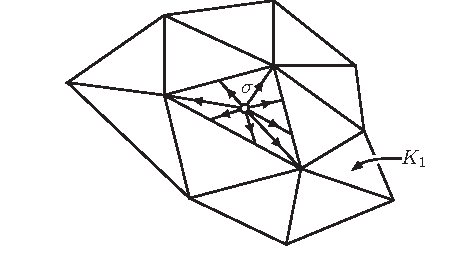
\includegraphics[width=.65\textwidth]{figures/4-7-1.pdf}\\图 4.7.1\end{center}

\textbf{步骤 2：}现在处理任意复形。仍只需证明 (1)，再由引理 4.7.2 得 (2)，由五引理得 (3)。

\sourcepage{225}
先证明满射性。给定 $\{z\}\in\widetilde H_p(|K|)$，奇异链 $z$ 的载体为紧集 $A$。取有限子复形 $L\subset K$，使 $A\subset|L|$。考虑交换图
\[
\begin{array}{ccc}
\widetilde H_p(\mathcal C'(L))&\xrightarrow[\cong]{\theta_*}&\widetilde H_p(|L|)\\
\downarrow\scriptstyle i_*&&\downarrow\scriptstyle j_*\\
\widetilde H_p(\mathcal C'(K))&\xrightarrow{\theta_*}&\widetilde H_p(|K|),
\end{array}
\]
其中竖直同态由包含映射诱导。类 $\{z\}$ 在 $j_*$ 的像中，而顶行由步骤 1 为同构，故 $\{z\}$ 在底行 $\theta_*$ 的像中。

再证明单射性。若 $\{z\}\in\widetilde H_p(\mathcal C'(K))$ 且 $\theta_*\{z\}=0$，则 $\theta z=\partial d$，其中 $d$ 为奇异 $(p+1)$ 维链。它的载体紧，故可取有限子复形 $L$，同时承载 $z$ 与 $d$。在上图中用这个 $L$，令 $\alpha\in\widetilde H_p(\mathcal C'(L))$ 为 $z$ 的类。由 $\theta z=\partial d$，顶行同构将 $\alpha$ 映为零，故 $\alpha=0$，于是 $\{z\}=i_*\alpha=0$。\translatornote{原书此处把顶行同态的定义域误印为 $H_p(\mathcal C'(K))$；实际应为 $\widetilde H_p(\mathcal C'(L))$。}\hfill$\square$

步骤 2 是所谓“正向极限论证”（direct limit argument）的一种典型形式，常用来把有限复形同调的结论推广到一般复形。

现在将这一引理与第 1.14 节的有序同调结果结合。

\entry{定义}{4.7.4}选取 $K$ 的顶点偏序，使其在每个单形的顶点上诱导全序，并按此序为单形定向。定义链映射 $\eta:\mathcal C(K)\to\mathcal S(|K|)$，令
\[
\eta([v_0,\ldots,v_p])=\ell(v_0,\ldots,v_p),\qquad v_0<\cdots<v_p.
\]
它保持增广并与包含映射可交换，因此也诱导相对链映射。实际上，$\eta$ 是复合
\[
\mathcal C(K)\xrightarrow{\varphi}\mathcal C'(K)\xrightarrow{\theta}\mathcal S(|K|),
\]
其中 $\varphi$ 是定理 1.14.16 的链等价。因为两者都诱导同调同构，$\eta$ 也如此；相对及约化同调中同样成立。

\sourcepage{226}
链映射 $\eta$ 依赖顶点的排序，但 $\eta_*$ 不依赖。因为 $\eta_*=\theta_*\varphi_*$，$\theta$ 显然不依赖排序，而 $\varphi_*$ 由定理 1.14.16 也不依赖排序。又因 $\eta$ 与包含映射可交换，之字形引理的自然性说明 $\eta_*$ 与 $\partial_*$ 可交换。

\entry{定理}{4.7.5}映射 $\eta_*$ 是单纯同调到奇异同调的良定义同构，且与边缘同态 $\partial_*$ 可交换。

\entry{定理}{4.7.6}同构 $\eta_*$ 与单纯映射诱导的同态可交换。

\textbf{证明：}设 $f:(K,K_0)\to(L,L_0)$ 为单纯映射。定理 1.14.18 已说明 $f_*$ 与 $\varphi_*$ 可交换。只需证明与 $\theta_*$ 可交换；事实上链层次已有此性质。

有序链上的诱导映射为 $f'_\#(w_0,\ldots,w_p)=(f(w_0),\ldots,f(w_p))$。而
\[
f_\#\theta(w_0,\ldots,w_p)=f\circ\ell(w_0,\ldots,w_p).
\]
右端先将 $\Delta_p$ 线性地映到由 $w_0,\ldots,w_p$ 张成的单形，再由 $f$ 线性地映到 $L$ 的一个单形。线性映射的复合仍线性，故它等于
\[
\ell(f(w_0),\ldots,f(w_p))=\theta(f(w_0),\ldots,f(w_p))=\theta f'_\#(w_0,\ldots,w_p).
\]
\hfill$\square$

对于连续映射 $h$，可用 $\eta_*^{-1}h_*\eta_*$ 定义其在单纯同调上诱导的同态，其中中间的 $h_*$ 为奇异同调诱导同态。下面证明这与第二章用单纯逼近定义的同态相同。

\entry{定理}{4.7.7}同构 $\eta_*$ 与连续映射诱导的同态可交换。

\sourcepage{227}
\textbf{证明：}设 $h:(|K|,|K_0|)\to(|L|,|L_0|)$ 连续。取 $h$ 与恒等映射的单纯逼近，分别为
\[
f:(K',K'_0)\to(L,L_0),\qquad g:(K',K'_0)\to(K,K_0).
\]
在单纯同调中，按定义 $h_*=f_*(g_*)^{-1}$。在奇异同调中，因 $g$ 同伦于恒等映射（定理 2.7.7），$g_*$ 是恒等同构；又因 $f$ 同伦于 $h$，有 $f_*=h_*$。所以奇异同调也满足同样公式。对 $f,g$ 应用上一定理，便得结论。\hfill$\square$

虽然已证明 $\eta$ 诱导同调同构，尚未找到其链同伦逆 $\lambda$。这样的逆确实存在，是后续结果的推论，见第 5.7 节习题。利用“正则邻域”理论还可得到 $\lambda$ 的具体公式，见 [ES52]。

\subsection*{习题}
\begin{enumerate}
\item 证明：若 $K_1,K_2$ 是复形 $K$ 的子复形，则 $\{|K_1|,|K_2|\}$ 为奇异同调中的可切除对。
\item 说明若 $K_1,K_2$ 不是子复形，则习题 1 的结论可能不成立。
\end{enumerate}

\section{*应用：局部同调群与流形}
\sourcepage{227--228}
本节定义空间在一点处的局部同调群，并用它证明关于流形的若干非平凡事实。全节假设 $X$ 是 Hausdorff 空间。本节将作为第八章的预备知识，第 4.12 节的一个例子也将用到它。

\entry{定义}{4.8.1}空间 $X$ 在点 $x\in X$ 处的\textbf{局部同调群}（local homology groups）是奇异同调群 $H_p(X,X\setminus\{x\})$。

\entry{引理}{4.8.2}若 $A\subset X$ 包含 $x$ 的一个邻域，则
\[
H_p(X,X\setminus\{x\})\cong H_p(A,A\setminus\{x\}).
\]
因此，若 $x\in X$、$y\in Y$ 分别有邻域 $U,V$，使 $(U,x)$ 与 $(V,y)$ 同胚，则两点处的局部同调群同构。这解释了“局部”一词。

\textbf{证明：}令 $U=X\setminus A$。因 $A$ 包含 $x$ 的邻域，$\overline U\subset X\setminus\{x\}=\Int(X\setminus\{x\})$。切除定理给出
\[
H_p(X,X\setminus\{x\})\cong H_p(X\setminus U,(X\setminus\{x\})\setminus U)=H_p(A,A\setminus\{x\}).
\]
\hfill$\square$

\entry{例}{4.8.3}若 $x\in\R^m$，则 $H_i(\R^m,\R^m\setminus\{x\})$ 在 $i=m$ 时为无限循环群，其余为零。取以 $x$ 为中心的正半径闭球 $B$。由上一个引理，
\[
H_i(\R^m,\R^m\setminus\{x\})\cong H_i(B,B\setminus\{x\})\cong H_i(B^m,B^m\setminus\{0\}).
\]
球面 $S^{m-1}$ 是 $B^m\setminus\{0\}$ 的形变收缩核（图 4.8.1，形变公式见定理 2.7.11 的证明），故最后一个群同构于 $H_i(B^m,S^{m-1})$。由定理 4.4.11 即得结论。

\entry{例}{4.8.4}记欧氏半空间
\[
\mathbb H^m=\{(x_1,\ldots,x_m):x_m\ge0\},\qquad \Bd\mathbb H^m=\R^{m-1}\times\{0\}.
\]
若 $x\in\Bd\mathbb H^m$，则所有 $H_i(\mathbb H^m,\mathbb H^m\setminus\{x\})$ 均为零；若 $x$ 在开上半空间内，则此群在 $i=m$ 时为无限循环群，其余为零。

对内部点，存在同时为 $\R^m$ 中开集的邻域，由上一例及引理 4.8.2 可得结论。对于边界点，可设 $x=0$。令 $D^m=B^m\cap\mathbb H^m$ 为闭半球体，它包含 $0$ 在半空间中的一个邻域，故
\[
H_i(\mathbb H^m,\mathbb H^m\setminus\{0\})\cong H_i(D^m,D^m\setminus\{0\}).
\]
\sourcepage{229}
\begin{center}
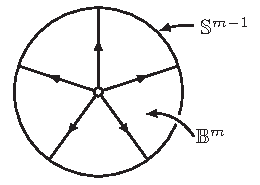
\includegraphics[width=.36\textwidth]{figures/4-8-1.pdf}\\图 4.8.1\par\medskip
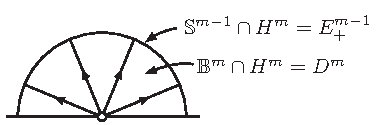
\includegraphics[width=.52\textwidth]{figures/4-8-2.pdf}\\图 4.8.2
\end{center}
从穿孔球到球面的径向形变收缩，限制为 $D^m\setminus\{0\}$ 到 $S^{m-1}\cap\mathbb H^m=E^{m-1}_+$ 的形变收缩。半球体 $D^m$ 为凸集，故无环；半球面 $E^{m-1}_+$ 同胚于 $B^{m-1}$，也无环。由长正合列，二者的相对同调为零，因而得到边界点处的结论。

\entry{定义}{4.8.5}若非空 Hausdorff 空间 $X$ 的每一点都有邻域同胚于 $\R^m$ 的开子集，则称它为\textbf{$m$ 维流形}（$m$-manifold）。若每一点都有邻域同胚于 $\mathbb H^m$ 的开子集，则称它为\textbf{带边界的 $m$ 维流形}（$m$-manifold with boundary）。

每个 $m$ 维流形自动是带边界的流形：若一点的邻域同胚于欧氏开集，可缩小为同胚于开球的邻域，再将此开球同胚地映到以 $(0,\ldots,0,1)$ 为中心的单位开球，它是半空间的开子集。

流形的定义常另外要求有可数基，或至少可度量化。本书不作这两项假设。流形及带边界流形是最熟悉、最重要的几何对象之一，也是微分几何和微分拓扑的主要研究对象。

\sourcepage{230}
若 $h:U\to V$ 将 $X$ 的开集同胚地映到 $\mathbb H^m$ 的开集，则称 $h$ 为 $X$ 上的\textbf{坐标片}（coordinate patch）。一点可能被映入开上半空间，也可能被映到边缘 $\R^{m-1}\times\{0\}$。局部同调区分这两种情况：前者的 $H_m(X,X\setminus\{x\})$ 为无限循环群，后者为零。这引出以下定义。

\entry{定义}{4.8.6}若带边界流形 $X$ 的点 $x$ 在一个坐标片下映入 $\Bd\mathbb H^m$，则在每个坐标片下都如此。称这样的点为 $X$ 的\textbf{边界点}，全体边界点组成的集合称为 $X$ 的\textbf{边界}，记作 $\Bd X$。称 $X\setminus\Bd X$ 为\textbf{内部}，记作 $\Int X$。

定义并不要求边界非空。若边界为空，$X$ 就是通常的 $m$ 维流形。但内部不能空：任一坐标片的像是半空间中的非空开集，必含开上半空间的点，相应的原像就是内部点。半空间 $\mathbb H^m$ 本身是带边界流形，其边界恰是 $\R^{m-1}\times\{0\}$；$\R^m$ 本身也是 $m$ 维流形。

\entry{定义}{4.8.7}由例 4.8.4，$m$ 由空间 $X$ 唯一决定：它是使 $H_m(X,X\setminus\{x\})$ 对至少一个 $x$ 非零的唯一整数。称 $m$ 为带边界流形 $X$ 的\textbf{维数}。

\entry{例}{4.8.8}单位球 $B^n$ 是带边界的 $n$ 维流形，且 $\Bd B^n=S^{n-1}$。若 $p\in B^n\setminus S^{n-1}$，开单位球直接给出坐标片。若 $p\in S^{n-1}$，至少一个坐标非零。不妨设 $p_n<0$。取 $U=\{x\in B^n:x_n<0\}$，定义
\[
h(x)=(x_1,\ldots,x_{n-1},x_n+f(x)),\qquad
f(x)=\sqrt{1-x_1^2-\cdots-x_{n-1}^2}.
\]
可验证 $h$ 将 $U$ 同胚地映到 $V=\{y\in\mathbb H^n:\|y\|<1\}$，且把 $p$ 映到半空间边界，见图 4.8.3。

\sourcepage{231}
\begin{center}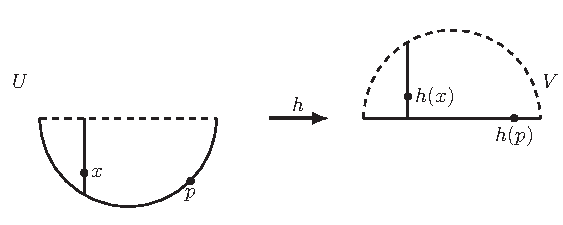
\includegraphics[width=.8\textwidth]{figures/4-8-3.pdf}\\图 4.8.3\end{center}
\entry{例}{4.8.9}任意 $n$ 维单形 $\sigma$ 同胚于 $B^n$，故为带边界的 $n$ 维流形。这个同胚把所有真面的并 $Y$ 映到 $S^{n-1}$。因此，原先记作 $\Bd\sigma$ 的 $Y$，恰为流形意义的边界；原先记作 $\Int\sigma$ 的 $\sigma\setminus Y$，恰为流形意义的内部。

这里有术语重叠，需要澄清。一般拓扑中，若 $A\subset X$，$A$ 的内部是包含于 $A$ 的所有 $X$ 中开集之并；边界是 $\overline A\cap\overline{X\setminus A}$。特别地，当 $A$ 开时，$\Bd A=\overline A\setminus A$。此前本书已用过这些概念，如引理 1.2.7 的 $\Bd U$，以及切除公理中的 $\Int A$。

流形的边界和内部是不同的概念。同一术语有两种用法颇不方便。有些作者用 $\partial X$ 表示流形边界，但这又不易与单纯链 $\partial\sigma$ 区分。我们只好依上下文辨明。对于 $B^n\subset\R^n$，这两种边界碰巧相同；$\mathbb H^n\subset\R^n$ 也是如此，但应把它们视为特殊情况。

下面证明一个关于流形三角剖分的结果。

\sourcepage{232}
\entry{引理}{4.8.10}若 $s$ 是复形 $K$ 的单形，$x,y\in\Int s$，则 $|K|$ 在 $x,y$ 处的局部同调群同构。

\textbf{证明：}只需证明 $x=\widehat s$ 为重心的情形。在第一次重心重分 $\operatorname{sd}K$ 的构造中，将 $s$ 的重心替换为 $y$，即从 $y$ 而非 $\widehat s$ 对 $\Bd s$ 的重分取星，得到重分 $K'$。存在从 $\operatorname{sd}K$ 到 $K'$ 的线性同构，将 $\widehat s$ 映到 $y$，其余顶点不动。因此空间偶 $(|K|,|K|\setminus\{\widehat s\})$ 与 $(|K|,|K|\setminus\{y\})$ 同胚。\hfill$\square$

回忆同胚 $h:|K|\to M$ 称为 $M$ 的\textbf{三角剖分}。任意流形能否三角剖分的问题，经历了约一个世纪的研究。初始猜想可追溯到 Poincar\'e 1899 年的论文，\footnote{Poincar\'e 的拓扑学著作译文见 [Poi10]；第 105--109 页与三角剖分有关。那里的论证尚不满足现代的严格性标准。}Kneser 的 1924 年论文 [Kne25] 为相关问题引入了“Hauptvermutung”这一名称。简言之，所有二维、三维拓扑流形均可三角剖分，而四维及更高维存在不可三角剖分的拓扑流形。较详细而简短的讨论见 [Man14]。

\entry{定理}{4.8.11}若 $M$ 为带边界的 $m$ 维流形，$h:|K|\to M$ 为同胚，则 $h^{-1}(\Bd M)$ 是 $K$ 的某个子复形的多面体。

\textbf{证明：}若开单形 $\Int s$ 与该集合相交，由上一个引理，它完全包含于该集合。因该集合闭，也包含 $s$。\hfill$\square$

最后应用局部同调证明：有限维单纯复形 $K$ 的维数是 $|K|$ 的拓扑不变量。第 2.4、2.7 节习题曾用覆盖维数给出另一种证明的轮廓。先证两个引理。

\entry{引理}{4.8.12}若 $v*L$ 是复形 $L$ 上的锥，则 $|L|$ 是 $|v*L|\setminus\{v\}$ 的形变收缩核。

\textbf{证明：}考虑商映射 $\pi:|L|\times I\to|v*L|$，$\pi(x,t)=(1-t)x+tv$（推论 2.8.8）。集合 $|L|\times[0,1)$ 开且饱和，因此其限制是到 $|v*L|\setminus\{v\}$ 的商映射。它一一对应，故为同胚。再由 $|L|\times\{0\}$ 是 $|L|\times[0,1)$ 的形变收缩核，即得结论。\hfill$\square$

\sourcepage{233}
回忆顶点 $v$ 的星 $\operatorname{St}v$ 是所有含 $v$ 为顶点的单形的内部之并，其链环为 $\operatorname{Lk}v=\overline{\operatorname{St}v}\setminus\operatorname{St}v$。

\entry{引理}{4.8.13}若 $v$ 是 $K$ 的顶点，则
\[
H_i(|K|,|K|\setminus\{v\})\cong H_i(\overline{\operatorname{St}v},\operatorname{Lk}v).
\]
\textbf{证明：}闭星包含 $v$ 的邻域，故引理 4.8.2 给出到 $H_i(\overline{\operatorname{St}v},\overline{\operatorname{St}v}\setminus\{v\})$ 的同构。令 $L$ 为多面体等于 $\operatorname{Lk}v$ 的子复形。由引理 1.9.4，闭星是锥 $v*L$ 的多面体，见图 4.8.4。由上一个引理，链环是穿孔闭星的形变收缩核，即得结论。\hfill$\square$
\begin{center}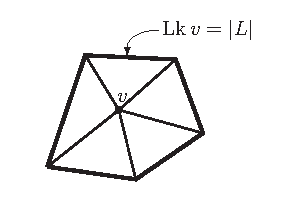
\includegraphics[width=.45\textwidth]{figures/4-8-4.pdf}\\图 4.8.4\end{center}

\entry{定理}{4.8.14}设 $K$ 为 $n$ 维复形，$X=|K|$。当 $p>n$ 时，每个局部同调群 $H_p(X,X\setminus\{x\})$ 都为零；而 $p=n$ 时，至少有一点 $x$ 使该群非零。

\textbf{证明：}取 $K$ 的一个 $n$ 维单形 $\sigma$。它不是其他单形的真面，故 $\Int\sigma$ 在 $|K|$ 中开：其补集为除 $\sigma$ 外所有单形之并。取 $x=\widehat\sigma$，引理 4.8.2 给出
\[
H_n(X,X\setminus\{x\})\cong H_n(\sigma,\sigma\setminus\{\widehat\sigma\})\cong H_n(B^n,B^n\setminus\{0\}),
\]
由例 4.8.3，后者为无限循环群。

对任意 $x$，由引理 4.8.10，只需考虑它是某个单形重心的情形。于是 $x$ 是 $L=\operatorname{sd}K$ 的顶点，由上一个引理，
\[
H_p(X,X\setminus\{x\})\cong H_p(\overline{\operatorname{St}(x,L)},\operatorname{Lk}(x,L)).
\]
\sourcepage{234}
\translatornote{原书此式左端下标误印为 $n$；应与右端同为 $p$。}右端可按奇异同调或单纯同调计算。闭星是维数至多为 $n$ 的复形的多面体，所以 $p>n$ 时，其相对单纯链群为零，同调为零，因而奇异同调也为零。\hfill$\square$

下面三个定义将在习题中使用。

\entry{定义}{4.8.15}若对任意 $x,y\in X$，都有 $X$ 到自身的同胚将 $x$ 映到 $y$，称 $X$ 为\textbf{齐性空间}（homogeneous space）。

\entry{定义}{4.8.16}若空间或复形的同调群与 $S^n$〔相应地，与 $B^n$〕相同，则称为\textbf{$n$ 维同调球面}（homology sphere）〔相应地，\textbf{同调球}（homology ball）〕。

\entry{定义}{4.8.17}\textbf{实心环面}（solid torus）是同胚于 $S^1\times B^2$ 的空间。它是带边界的三维流形，边界同胚于环面。

\subsection*{习题}
\begin{enumerate}
\item 验证例 4.8.8 的细节。
\item 证明：若 $M,N$ 分别为 $m,n$ 维带边界流形，则 $M\times N$ 为 $m+n$ 维带边界流形，且
\[
\Bd(M\times N)=(M\times\Bd N)\cup(\Bd M\times N).
\]
\item 证明连通流形是齐性的。〔提示：若有自身同胚把 $x$ 映到 $y$，定义 $x\sim y$。证明这是等价关系，且每个等价类开。〕
\item 设 $h:|K|\to M$ 是带边界的 $m$ 维流形的三角剖分。
\begin{enumerate}[label=(\alph*)]
\item 证明：顶点 $v$ 的链环在 $h(v)\in\Int M$ 时是 $(m-1)$ 维同调球面，在 $h(v)\in\Bd M$ 时是同调球。
\item 证明 $K$ 的每个单形或为 $m$ 维，或是某个 $m$ 维单形的面。
\item 证明：若 $(m-1)$ 维单形 $s\subset h^{-1}(\Bd M)$，则它恰是一个 $m$ 维单形的面；否则恰是两个 $m$ 维单形的面。
\end{enumerate}
\item 利用 $S^3$ 同胚于 $\Bd(B^2\times B^2)$，把 $S^3$ 写成两个实心环面 $T_1,T_2$ 之并，使其交为共同边界。计算相应 Mayer--Vietoris 序列。
\item 设 $C$ 为实数轴中的 Cantor 三分集（定义 2.3.13）。$C$ 的维数是多少？
\item 给出 $\R^3$ 中一个一维集合的例子，再给出一个二维集合的例子。
\end{enumerate}

\section{*应用：Jordan 曲线定理}
\sourcepage{235}
利用奇异同调的基本性质，现在证明若干经典拓扑定理，包括广义 Jordan 曲线定理与 Brouwer 区域不变性定理。

\entry{定义}{4.9.1}若子空间 $A\subset X$ 使 $X\setminus A$ 不连通，则称 $A$ \textbf{分离}（separates）$X$。

我们主要考虑 $X=\R^n$ 或 $S^n$，且 $A$ 闭的情形。此时补空间局部道路连通，故其连通分支与道路分支相同。特别地，$\widetilde H_0(X\setminus A)=0$ 当且仅当补空间连通；一般来说，这个群的秩等于分支数减一。下文将自由使用这一事实。

\entry{定义}{4.9.2}同胚于单位球 $B^k$ 的空间称为\textbf{$k$ 维胞腔}（$k$-cell）。

\entry{定理}{4.9.3}若 $B$ 是 $S^n$ 中的 $k$ 维胞腔，则 $S^n\setminus B$ 无环。特别地，$B$ 不分离 $S^n$。

\textbf{证明：}固定 $n$，对 $k$ 归纳。若 $k=0$，$B$ 为单点。其补空间在 $n=0$ 时为单点，在 $n>0$ 时同胚于 $\R^n$，均无环。设结论对 $(k-1)$ 维胞腔成立，取同胚 $h:I^k\to B$。

\sourcepage{236}
\textbf{步骤 1：}令
\[
B_0=h(I^{k-1}\times[0,\tfrac12]),\quad B_1=h(I^{k-1}\times[\tfrac12,1]),\quad
C=h(I^{k-1}\times\{\tfrac12\}).
\]
前两者为 $k$ 维胞腔，$C$ 为 $(k-1)$ 维胞腔，见图 4.9.1。我们证明：若 $0\ne\alpha\in\widetilde H_i(S^n\setminus B)$，则它在至少一个包含映射 $S^n\setminus B\to S^n\setminus B_0$、$S^n\setminus B\to S^n\setminus B_1$ 下的像非零。

令 $X=S^n\setminus C$，由归纳假设它无环。取开集 $X_0=S^n\setminus B_0$、$X_1=S^n\setminus B_1$，则 $X=X_0\cup X_1$，且 $A=X_0\cap X_1=S^n\setminus B$。Mayer--Vietoris 序列给出
\[
\widetilde H_{i+1}(X)\longrightarrow\widetilde H_i(A)\longrightarrow
\widetilde H_i(X_0)\oplus\widetilde H_i(X_1)\longrightarrow\widetilde H_i(X).
\]
两端为零，故中间同态为同构。它将 $\alpha$ 映为 $(i_*\alpha,-j_*\alpha)$，因此两个分量至少一个非零。
\begin{center}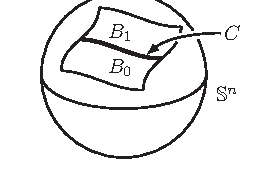
\includegraphics[width=.42\textwidth]{figures/4-9-1.pdf}\\图 4.9.1\end{center}

\textbf{步骤 2：}反设存在上述非零 $\alpha$。根据步骤 1，二等分 $[0,1]$ 后可选其中一个闭区间 $[a_1,b_1]$，长度为 $2^{-1}$，使 $\alpha$ 在 $\widetilde H_i(S^n\setminus D_1)$ 中的像非零，其中 $D_1=h(I^{k-1}\times[a_1,b_1])$。

\sourcepage{237}
再次把该区间二等分，选取使像非零的一半。继续便得到套叠闭区间
\[
[a_1,b_1]\supset[a_2,b_2]\supset\cdots,\qquad b_m-a_m=2^{-m},
\]
及 $D_m=h(I^{k-1}\times[a_m,b_m])$，使 $\alpha$ 在每个 $\widetilde H_i(S^n\setminus D_m)$ 中的像都非零。\translatornote{原书第二次二等分所写的一个端点 $b_2$ 应为 $b_1$；此处统一按递归区间表达。}

设 $\bigcap_m[a_m,b_m]=\{e\}$，则 $E=h(I^{k-1}\times\{e\})=\bigcap_mD_m$ 是 $(k-1)$ 维胞腔。归纳假设给出 $\widetilde H_i(S^n\setminus E)=0$。因此 $\alpha$ 的像在此为零。由定理 4.3.5，存在 $S^n\setminus E$ 中的紧子集 $A$，使 $\alpha$ 已在 $\widetilde H_i(A)$ 中变为零。可先把代表 $\alpha$ 的有限链载体包含在这个紧集内。

但是 $S^n\setminus E$ 是递增开集 $S^n\setminus D_m$ 之并，故紧集 $A$ 包含于其中一个。于是 $\alpha$ 在相应同调群中的像为零，与构造矛盾。\hfill$\square$

\entry{定理}{4.9.4}设 $n>k\ge0$，$h:S^k\to S^n$ 为嵌入，则
\[
\widetilde H_i(S^n\setminus h(S^k))=\begin{cases}\Z,&i=n-k-1,\\0,&\text{其他情形}.\end{cases}
\]
\textbf{证明：}固定 $n$，对 $k$ 归纳。若 $k=0$，像为两点 $p,q$，其补空间同胚于 $\R^n\setminus\{0\}$，而后者同伦等价于 $S^{n-1}$，故结论成立。

设结论对 $k-1$ 成立。取开集 $X_1=S^n\setminus h(E^k_+)$、$X_2=S^n\setminus h(E^k_-)$。令
\[
X=X_1\cup X_2=S^n\setminus h(S^{k-1}),\qquad A=X_1\cap X_2=S^n\setminus h(S^k).
\]
Mayer--Vietoris 序列给出
\[
\begin{split}
\widetilde H_{i+1}(X_1)\oplus\widetilde H_{i+1}(X_2)\longrightarrow
\widetilde H_{i+1}(X)\longrightarrow\widetilde H_i(A)\\
\longrightarrow\widetilde H_i(X_1)\oplus\widetilde H_i(X_2).
\end{split}
\]
\sourcepage{238}
\begin{center}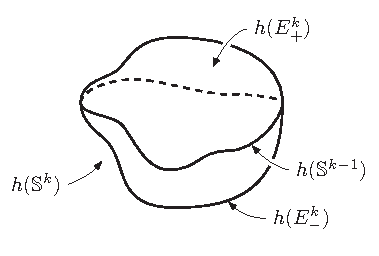
\includegraphics[width=.55\textwidth]{figures/4-9-2.pdf}\\图 4.9.2\end{center}
两个半球的像都是胞腔，所以上一定理说明 $X_1,X_2$ 无环。于是中间映射为同构，亦即
\[
\widetilde H_{i+1}(S^n\setminus h(S^{k-1}))\cong\widetilde H_i(S^n\setminus h(S^k)).
\]
由归纳假设，左端只在 $i+1=n-(k-1)-1$ 时为无限循环群，其余为零，即得结论。\hfill$\square$

\entry{定理}{4.9.5（广义 Jordan 曲线定理）}设 $n>0$，$C\subset S^n$ 同胚于 $S^{n-1}$。则 $S^n\setminus C$ 恰有两个连通分支，$C$ 是二者共同的拓扑边界。

\textbf{证明：}对上一定理取 $k=n-1$，得 $\widetilde H_0(S^n\setminus C)\cong\Z$，故补空间恰有两个道路分支，也就是连通分支 $W_1,W_2$。它们在 $S^n$ 中开，故边界分别为 $\overline W_i\setminus W_i$。只需证明 $\overline W_1\setminus W_1=C$。

由于 $W_2$ 开，它的点不可能是 $W_1$ 的极限点，所以 $\overline W_1\subset S^n\setminus W_2=W_1\cup C$，从而 $\overline W_1\setminus W_1\subset C$。\translatornote{原书此处将 $W_1\cup C$ 误印为 $W_1\cap C$。}

反过来，给定 $x\in C$ 及其邻域 $U$，只需证明它与闭集 $\overline W_1\setminus W_1$ 相交。将 $C$ 分成两个 $(n-1)$ 维胞腔 $C_1,C_2$，使 $C_1$ 足够小而包含于 $U$。图 4.9.3 表示 $n=2$ 的情形。

因为 $C_2$ 不分离 $S^n$，可在 $S^n\setminus C_2$ 中取道路 $\alpha$，连接 $p\in W_1$ 与 $q\in W_2$。该道路必经过 $\overline W_1\setminus W_1$：否则它包含于两个不交开集 $W_1$ 和 $S^n\setminus\overline W_1$ 之并，并同时与两者相交，违背道路像的连通性。

\sourcepage{239}
\begin{center}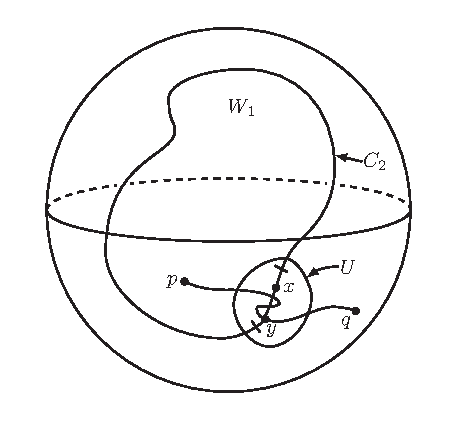
\includegraphics[width=.68\textwidth]{figures/4-9-3.pdf}\\图 4.9.3\end{center}
取道路上的边界点 $y$，则 $y\in C$，且 $y\notin C_2$，故 $y\in C_1\subset U$。因此每个 $U$ 都与该闭边界相交，即得另一包含关系。\hfill$\square$

$S^n$ 的赤道是 $S^{n-1}$ 的同胚像，其补空间两个分支都是开球，闭包都是 $n$ 维胞腔。于是可能猜想，上一定理中的 $\overline W_1,\overline W_2$ 总是 $n$ 维胞腔。$n=2$ 时确实如此，称为 \textbf{Schoenflies 定理}，证明见 [New51]。但 $n>2$ 时需要附加条件。$n\ge3$ 时的广义 Schoenflies 定理由 M. Brown 和 B. Mazur 独立证明，相关论文为 [Maz59]、[Maz61]、[Bro60]、[Mor60]。

三维及更高维中的困难由 J. W. Alexander 于 1924 年在 [Ale24] 中揭示。他构造了后来称为 \textbf{Alexander 角球}（Alexander horned sphere）的曲面。先从环面删去一段，如图 4.9.4 上部，再用圆盘补上两个洞，得到同胚于球面的曲面。接着取两个较小的不完整环面，通过从圆盘小孔伸出的管道，将它们分别接到两张圆盘上。无限重复这一过程。图的下部取自 Alexander 原文，原标记已遮去以免杂乱。

\sourcepage{240}
\begin{center}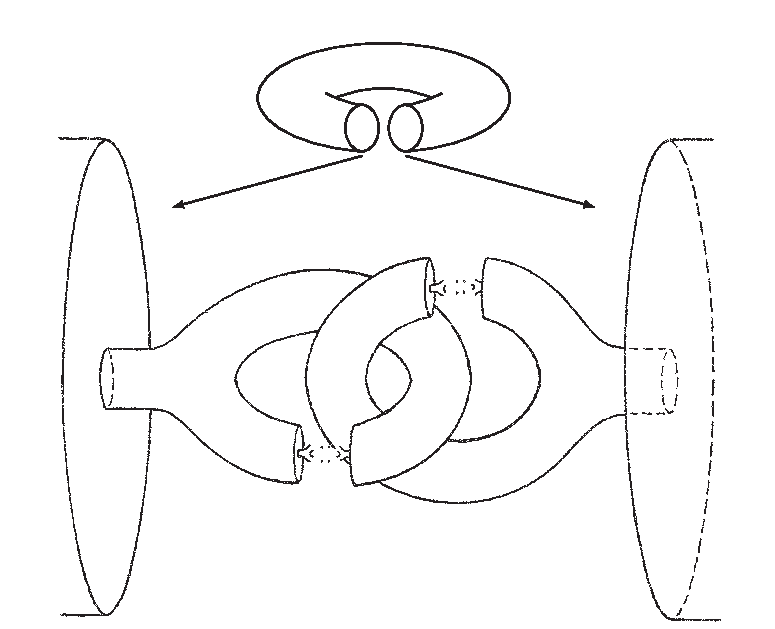
\includegraphics[width=.96\textwidth]{figures/4-9-4.pdf}\\图 4.9.4：Alexander 角球\end{center}
最终曲面同胚于二维球面，但在空间中的嵌入方式与普通圆球面很不相同。若让一条闭曲线穿过其中某个不完整环面看似存在的洞，就不能在始终不碰到角球的条件下把它缩为一点。

经典 Jordan 曲线定理通常对嵌入 $\R^n$ 的球面陈述，而不是嵌入 $S^n$ 的球面。\footnote{长期以来常有人说 Jordan 未成功证明以其命名的定理。其法文原始论述见 [Jor14] 第 587--594 页，读者可自行研究并判断论证的有效性。}下面证明这一版本。

\entry{推论}{4.9.6}设 $n\ge2$，$C\subset\R^n$ 同胚于 $S^{n-1}$。则 $\R^n\setminus C$ 恰有两个连通分支，$C$ 为二者共同的拓扑边界。

\sourcepage{241}
\textbf{证明：步骤 1。}先证明 $S^n$ 的连通开集 $U$ 中，没有一点能够分离 $U$。反设 $U\setminus\{p\}$ 不连通。取足够小的开球 $B(p,\varepsilon)\subset U$，其穿孔部分同胚于 $\R^n\setminus\{0\}$，因 $n\ge2$ 而连通，故包含于某一分支 $D$。令 $E$ 为其余分支之并，则 $E$ 非空，且 $p$ 不是 $E$ 的极限点。因此 $D\cup\{p\}$ 与 $E$ 是不交、非空、开且并为 $U$ 的集合，与连通性矛盾。

\textbf{步骤 2。}将 $\R^n$ 视为 $S^n\setminus\{p\}$，其中 $p$ 为北极。由上一定理，$S^n\setminus C$ 有两个分支 $W_1,W_2$，可设 $p\in W_1$。由步骤 1，$W_1\setminus\{p\}$ 连通，所以它与 $W_2$ 恰为 $(S^n\setminus\{p\})\setminus C$ 的两个分支。它们在该空间中的边界均为 $C$。\hfill$\square$

\entry{定理}{4.9.7（区域不变性）}设 $U\subset\R^n$ 开，$f:U\to\R^n$ 连续且单射。则 $f(U)$ 在 $\R^n$ 中开，且 $f:U\to f(U)$ 是同胚。

\textbf{证明：}可以用 $S^n$ 代替 $\R^n$。

\textbf{步骤 1。}给定 $y\in f(U)$，令 $f(x)=y$。取足够小的开球 $B(x,\varepsilon)$，使闭包 $\overline{B(x,\varepsilon)}\subset U$。记球面 $S(x,\varepsilon)=\overline{B(x,\varepsilon)}\setminus B(x,\varepsilon)$，见图 4.9.5。连续单射在这个紧球上的限制是嵌入，因此 $f(S(x,\varepsilon))$ 同胚于 $S^{n-1}$。由定理 4.9.5，其补空间有两个开分支 $W_1,W_2$。

集合 $f(B(x,\varepsilon))$ 连通且与该球面不交，可设它包含于 $W_1$。它必须等于 $W_1$；否则
\[
S^n\setminus\bigl[f(B(x,\varepsilon))\cup f(S(x,\varepsilon))\bigr]
=S^n\setminus f(\overline{B(x,\varepsilon)})
\]
同时含有整个 $W_2$ 及 $W_1$ 的一些点，因而不连通。这与定理 4.9.3 矛盾，因为 $f(\overline{B(x,\varepsilon)})$ 是一个胞腔。因此 $f(U)$ 包含 $y$ 的开邻域 $W_1$，从而为开集。

\textbf{步骤 2。}将步骤 1 用于 $U$ 的每个开子集，说明 $f$ 是开映射，因此是到其像的同胚。\hfill$\square$

\sourcepage{242}
\begin{center}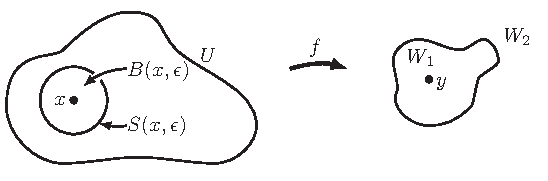
\includegraphics[width=.8\textwidth]{figures/4-9-5.pdf}\\图 4.9.5\end{center}
若额外假设 $f$ 连续可微且 Jacobian 非奇异，区域不变性可由分析中的反函数定理较容易地推出。它的深刻之处是只需要连续性和单射性。同样，当嵌入 $S^{n-1}\to\R^n$ 是某个三角剖分上的单纯映射，或是 Jacobian 具有最大秩的可微映射时，Jordan 曲线定理也较容易证明；真正的困难在于只假设连续且单射。

\subsection*{习题}
\begin{enumerate}
\item 设 $M$ 是第 4.8 节定义的带边界 $m$ 维流形。利用区域不变性证明：
\begin{enumerate}[label=(\alph*)]
\item 若一点在一个坐标片下映到 $\R^{m-1}\times\{0\}$，则在每个坐标片下都如此。
\item 若 $U\subset\R^m$、$V\subset\R^n$ 为非空开集且彼此同胚，则 $m=n$。
\item 数 $m$ 由 $M$ 唯一确定。
\end{enumerate}
\item \begin{enumerate}[label=(\alph*)]
\item 设 $Y$ 为拓扑学家的正弦曲线（定义 4.2.11）。证明：若 $h:Y\to S^n$ 为嵌入，则 $S^n\setminus h(Y)$ 无环。
\item 设 $X$ 为闭合的拓扑学家正弦曲线（定义 4.6.5）。证明：若 $h:X\to S^n$ 为嵌入，则 $\widetilde H_i(S^n\setminus h(X))$ 在 $i=n-2$ 时为无限循环群，其余为零。
\item 设 $X$ 同 (b)，若 $h:X\to S^2$ 为嵌入，证明其补空间恰有两个分支，且 $h(X)$ 为共同拓扑边界。
\end{enumerate}
\sourcepage{243}
\begin{center}
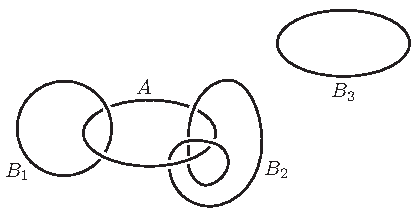
\includegraphics[width=.65\textwidth]{figures/4-9-6.pdf}\\图 4.9.6\par\medskip
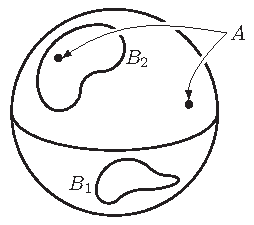
\includegraphics[width=.4\textwidth]{figures/4-9-7.pdf}\\图 4.9.7
\end{center}
\item \begin{enumerate}[label=(\alph*)]
\item 将 $S^3$ 视为添加了无穷远点的 $\R^3$。设 $A,B_1,B_2,B_3$ 为图 4.9.6 中的简单闭曲线。包含映射诱导的 $H_1(B_i)\to H_1(S^3\setminus A)$ 是无限循环群间的同态，因而为乘以一个除符号外确定的整数 $d_i$。它度量 $B_i$ 与 $A$ 环绕的次数。分别求这些整数；再求 $H_1(A)\to H_1(S^3\setminus B_i)$ 的相应整数。你能提出什么猜想？
\item 设 $A$ 为 $S^2$ 的两个点，$B_1,B_2$ 为图 4.9.7 中的简单闭曲线。求包含映射诱导的同态
\[
\widetilde H_0(A)\to\widetilde H_0(S^2\setminus B_i),\qquad H_1(B_i)\to H_1(S^2\setminus A),
\]
并提出猜想。
\item 对 $S^{p+q+1}$ 中不相交的 $S^p,S^q$ 的嵌入提出一个猜想。证明 Alexander 对偶定理后将再次讨论它，见第 8.12 节习题。
\end{enumerate}
\item 在三维中，对边界曲面作适当光滑性假设，可以得到 Jordan 曲线定理的一种加强形式。这是 Mazur 与 Brown 的著名结果。讨论可能的表述。
\end{enumerate}

\section{基本群}
\sourcepage{244}
本节简要介绍同伦论，特别考察空间的基本群。同伦论的一个动机是识别并分类拓扑空间中的“洞”。圆环中心有洞，单位球面也有洞（图 4.10.1），但直觉上它们性质不同，或许具有不同维数。同伦论帮助我们整理这些想法。
\begin{center}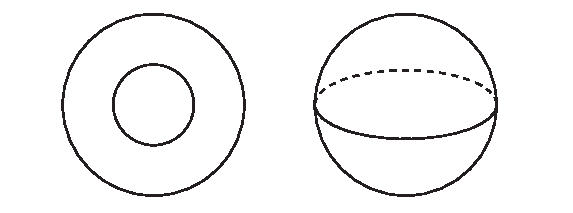
\includegraphics[width=.75\textwidth]{figures/4-10-1.pdf}\\图 4.10.1：不同类型的洞\end{center}
同伦论的出发点是空间 $X$ 中的所有\textbf{闭路}（loops）：即满足 $\gamma(0)=\gamma(1)$ 的连续映射 $\gamma:[0,1]\to X$。
\begin{center}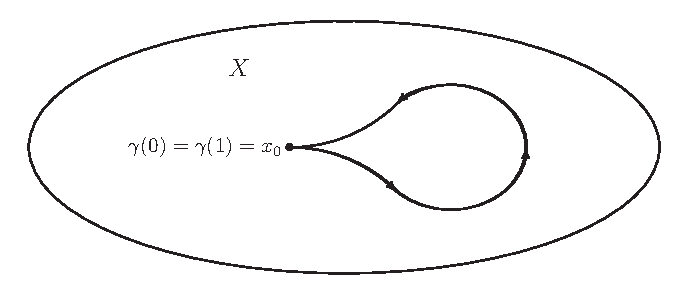
\includegraphics[width=.88\textwidth]{figures/4-10-2.pdf}\\图 4.10.2：$X$ 中的闭路\end{center}

\sourcepage{245}
\entry{定义}{4.10.1}固定 $x_0\in X$ 为\textbf{基点}（base point）。设 $\gamma_1,\gamma_2:[0,1]\to X$ 都以 $x_0$ 为起点和终点。若存在连续映射 $\Gamma:[0,1]\times[0,1]\to X$，满足
\begin{enumerate}[label=(\arabic*)]
\item $\Gamma(t,0)=\gamma_1(t)$，$0\le t\le1$；
\item $\Gamma(t,1)=\gamma_2(t)$，$0\le t\le1$；
\item $\Gamma(0,u)=x_0$，$0\le u\le1$；
\item $\Gamma(1,u)=x_0$，$0\le u\le1$，
\end{enumerate}
则称两闭路\textbf{保持基点同伦}（base-point homotopic），记为 $\gamma_1\simeq\gamma_2$，称 $\Gamma$ 为同伦映射。
\begin{center}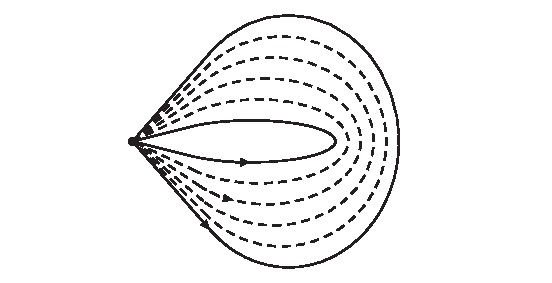
\includegraphics[width=.75\textwidth]{figures/4-10-3.pdf}\\图 4.10.3：两条同伦闭路\end{center}
图中还显示形变经过的一些中间闭路。图 4.10.4 则表示圆环中两条不能同伦的闭路；当然，“看起来不能同伦”还不等于证明它们不能同伦。

前两个条件说明它们作为映射同伦，后两个则要求形变中保持基点。因此这比定义 2.7.1 更强，但仍使用相同记号，由上下文区分。通常也简称“同伦”，不再提及基点。讨论和计算中，基点往往隐含不写。也有不固定基点的同伦理论，但这里介绍的是最常用的版本。

\sourcepage{246}
\begin{center}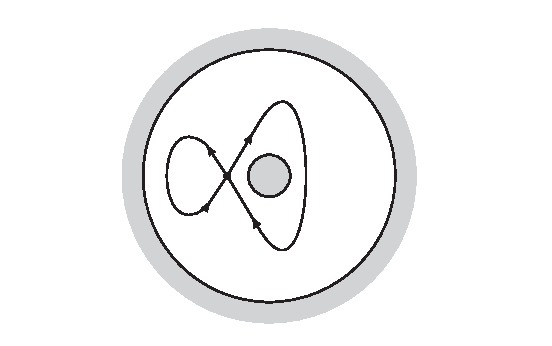
\includegraphics[width=.75\textwidth]{figures/4-10-4.pdf}\\图 4.10.4：圆环中两条不能同伦的闭路\end{center}
\entry{例}{4.10.2}设 $X$ 为欧氏空间的子集，$\gamma_1,\gamma_2$ 是具有同一基点的闭路。若对每个 $t$，从 $\gamma_1(t)$ 到 $\gamma_2(t)$ 的线段均在 $X$ 内，则
\[
\Gamma(t,u)=(1-u)\gamma_1(t)+u\gamma_2(t)
\]
给出保持基点的同伦。

\entry{引理}{4.10.3}定义 4.10.1 的关系在所有以 $x_0$ 为基点的闭路上是等价关系。

\textbf{证明：}自反性、对称性容易验证，只证传递性。若 $\Gamma_{12}$ 是从 $\gamma_1$ 到 $\gamma_2$ 的同伦，$\Gamma_{23}$ 是从 $\gamma_2$ 到 $\gamma_3$ 的同伦，令
\[
\Gamma_{13}(t,u)=\begin{cases}\Gamma_{12}(t,2u),&0\le u\le\tfrac12,\\\Gamma_{23}(t,2u-1),&\tfrac12\le u\le1.\end{cases}
\]
在接缝处两式都为 $\gamma_2(t)$，故映射良定义且连续。其端点值符合要求，给出从 $\gamma_1$ 到 $\gamma_3$ 的同伦。\hfill$\square$

\entry{定义}{4.10.4}闭路的等价类称为\textbf{同伦类}，$\gamma$ 的类记为 $[\gamma]$。这些类组成的集合称为第一同伦空间。定义乘积
\[
[\gamma]\cdot[\eta]=[\gamma\cdot\eta],\qquad
(\gamma\cdot\eta)(t)=\begin{cases}\gamma(2t),&0\le t\le\tfrac12,\\\eta(2t-1),&\tfrac12<t\le1.\end{cases}
\]
\sourcepage{247}
也就是说，先走 $\gamma$，再走 $\eta$，见图 4.10.5。下面将证明这使同伦类构成群，称为 $X$ 的\textbf{第一同伦群}或\textbf{基本群}（fundamental group），记为 $\pi_1(X,x_0)$，或简记 $\pi_1(X)$。我们采用乘法记号，单位元记为 $1$。
\begin{center}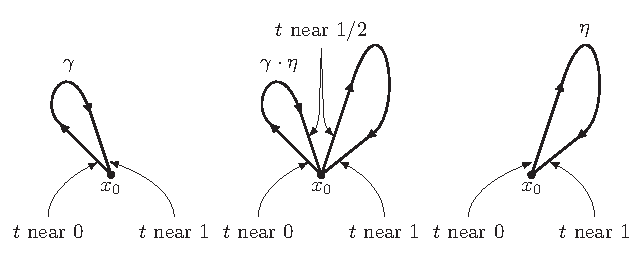
\includegraphics[width=.9\textwidth]{figures/4-10-5.pdf}\\图 4.10.5：$\gamma$ 与 $\eta$ 的乘积\end{center}

\entry{引理}{4.10.5}令 $\gamma_0(t)=x_0$ 为常值闭路，则：
\begin{enumerate}[label=(\arabic*)]
\item 上述乘法良定义；
\item 乘法满足结合律；
\item $[\gamma][\gamma_0]=[\gamma_0][\gamma]=[\gamma]$；
\item 若 $\eta(t)=\gamma(1-t)$，则 $[\gamma][\eta]=[\eta][\gamma]=[\gamma_0]$。
\end{enumerate}
\sourcepage{248}
\textbf{证明：}(1) 若 $\Gamma$ 给出 $\gamma\simeq\gamma'$，$\Phi$ 给出 $\eta\simeq\eta'$，则
\[
\Pi(t,u)=\begin{cases}\Gamma(2t,u),&0\le t\le\tfrac12,\ 0\le u\le1,\\\Phi(2t-1,u),&\tfrac12\le t\le1,\ 0\le u\le1\end{cases}
\]
是从 $\gamma\cdot\eta$ 到 $\gamma'\cdot\eta'$ 的同伦，见图 4.10.6。\translatornote{原书第二行把 $u$ 的上限误印为 $1/2$，应为 $1$。}其余三点也容易，留作习题。\hfill$\square$
\begin{center}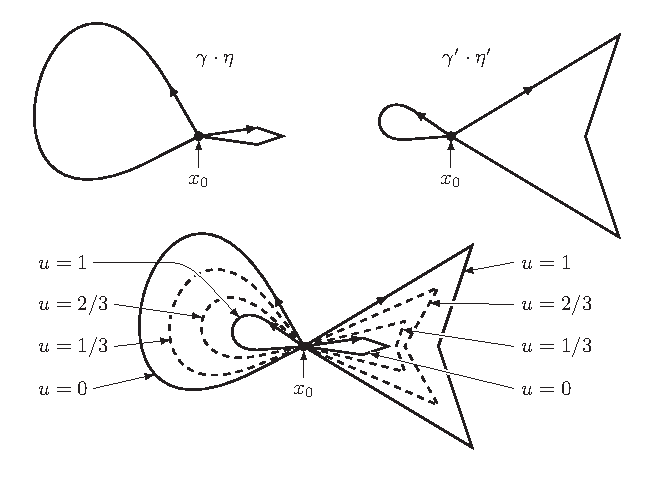
\includegraphics[width=.88\textwidth]{figures/4-10-6.pdf}\\图 4.10.6：乘积闭路间的同伦\end{center}
因此这确实是同伦类集合上的群运算。还有高阶同伦群 $\pi_k(X)$，但本书此处不讨论。基本群的重要性质是函子性。

\entry{定理}{4.10.6}若 $f:X\to Y$ 连续且 $f(x_0)=y_0$，则
\[
f_*:\pi_1(X,x_0)\to\pi_1(Y,y_0),\qquad f_*[\gamma]=[f\circ\gamma]
\]
是群同态。

\sourcepage{249}
\textbf{证明：}若 $\Gamma$ 是两闭路间的同伦，则 $f\circ\Gamma$ 是复合闭路间的同伦，所以良定义。又由分段定义，
\[
f\circ(\gamma\cdot\eta)=(f\circ\gamma)\cdot(f\circ\eta),
\]
故 $f_*([\gamma][\eta])=f_*[\gamma]f_*[\eta]$。\hfill$\square$

原书接着声称：“若 $f$ 单射，则 $f_*$ 单射；若 $f$ 满射，则 $f_*$ 满射。”\translatornote{这两句话一般都不成立。例如包含 $S^1\hookrightarrow B^2$ 是单射，却在基本群上诱导 $\Z\to0$；满射 $[0,1]\to S^1$，$t\mapsto e^{2\pi it}$，在基本群上诱导 $0\to\Z$。下面的拓扑不变性应由恒等与复合的函子性质，以及同胚的逆映射推出。}

\entry{推论}{4.10.7}基本群是空间的拓扑不变量。

因此同胚空间有同构的基本群；基本群不同构的空间不可能同胚。回忆单纯同调的定义与拓扑不变性证明曾需要很多准备，而基本群在几页之内就定义并证明了不变性。不过，计算基本群时，同伦论就变得更具挑战。

\entry{命题}{4.10.8}圆周的基本群同构于整数群：$\pi_1(S^1)\cong\Z$。

\textbf{证明：}把 $S^1$ 视为 $\{z\in\mathbb C:|z|=1\}$，基点取 $1$，记 $I=[0,1]$。闭路 $\sigma:I\to S^1$ 满足 $\sigma(0)=\sigma(1)=1$。令
\[
\varphi:\R\to S^1,\quad\varphi(x)=e^{2\pi ix},\qquad
\rho_n(t)=\varphi(nt)=e^{2\pi int}\quad(n\in\Z).
\]
若 $n>0$，$\rho_n$ 逆时针绕圆周 $n$ 圈；若 $n<0$，顺时针绕 $|n|$ 圈；$\rho_0$ 为常值闭路。

\sourcepage{250}
先证明每条 $\sigma$ 都同伦于某个 $\rho_n$。希望找到连续映射 $\sigma':I\to\R$，满足 $\sigma=\varphi\sigma'$、$\sigma'(0)=0$。于是 $\sigma'(1)=n\in\Z$，而
\[
\Gamma(t,u)=\varphi\bigl((1-u)\sigma'(t)+unt\bigr)
\]
就是从 $\sigma$ 到 $\rho_n$ 的同伦。称 $\sigma'$ 为 $\sigma$ 的\textbf{提升}（lifting），即使 $\varphi\sigma'=\sigma$ 的图交换。

形式上，似乎可以令 $\sigma'(t)=(2\pi i)^{-1}\log\sigma(t)$，但闭路通常绕遍圆周，无法全局使用单值对数。诀窍是：$\varphi$ 将 $(-1/2,1/2)$ 同胚地映到 $S^1\setminus\{-1\}$，其逆在这个集合上良定义。

由 $\sigma$ 在紧区间上的一致连续性，可取 $\varepsilon>0$，使 $|t-t'|<\varepsilon$ 时 $|\sigma(t)-\sigma(t')|<1$，于是 $\sigma(t)/\sigma(t')\ne-1$。\translatornote{原书在本段一致连续性的主语处两次误写为 $\varphi$，此处实际用的是 $\sigma$。}取 $K$ 使 $1/K<\varepsilon$，令 $p_i=i/K$，定义
\[
\sigma'(t)=\sum_{i=0}^{K-1}\varphi^{-1}\left(\frac{\sigma(tp_{i+1})}{\sigma(tp_i)}\right).
\]
各项因 $|tp_{i+1}-tp_i|<\varepsilon$ 而有意义，且连续。指数把和变为积，所以
\[
\varphi(\sigma'(t))=\prod_{i=0}^{K-1}\frac{\sigma(tp_{i+1})}{\sigma(tp_i)}
=\frac{\sigma(tp_K)}{\sigma(tp_0)}=\sigma(t).
\]

\sourcepage{251}
同样可提升同伦 $F:I\times I\to S^1$。取一致连续性参数 $\varepsilon$，令 $1/K<\varepsilon/2$，定义
\[
F'(t,u)=\sum_{i=0}^{K-1}\varphi^{-1}\left(\frac{F(tp_{i+1},up_{i+1})}{F(tp_i,up_i)}\right).
\]
因为
\[
\|(tp_{i+1},up_{i+1})-(tp_i,up_i)\|
\le |u(p_{i+1}-p_i)|+|t(p_{i+1}-p_i)|<\varepsilon,
\]
公式有意义，且 $\varphi F'=F$。若 $F$ 连接 $\rho_m$ 与 $\rho_n$，则 $F'(1,0)=m$、$F'(1,1)=n$。函数 $F'(1,u)$ 连续且取整数值，故为常值，得 $m=n$。因此各 $[\rho_n]$ 不同。最后验证 $[\rho_m][\rho_n]=[\rho_{m+n}]$ 即完成证明，这一步留作习题。\hfill$\square$

\entry{例}{4.10.9}若 $X$ 同胚于欧氏空间的凸子集，则 $\pi_1(X)=1$。由拓扑不变性，可设 $X$ 本身凸。固定基点 $x_0$，任一闭路与常值闭路由例 4.10.2 的线性同伦连接，故所有类都是单位元。这里用 $1$ 而非 $\{1\}$ 简记平凡乘法群。

若 $\pi_1(X)=1$，本书称 $X$ \textbf{单连通}（simply connected）。

\entry{例}{4.10.10}当 $n\ge2$ 时，$\pi_1(S^n)=1$。以 $n=2$ 为例。不能直接断言每条闭路的像包含于同胚于平面圆盘的球面子集：Peano 于 1890 年构造了空间填充曲线，闭路的像甚至可能覆盖整个球面。\footnote{原论文为 [Pea90]；Hilbert 在 [Hil91] 中给出了有帮助的图。英文说明见 [Mun00] 第 44 节。}不过，总可通过同伦修改闭路，使新闭路包含于这样的子集中。细节留作习题。

\sourcepage{252}
\subsection*{与同调的关系}
回忆奇异 $p$ 维单形是 $T:\Delta_p\to X$，其中 $\Delta_p$ 是 $\R^\infty$ 中顶点为 $\epsilon_0=0,\epsilon_1,\ldots,\epsilon_p$ 的标准单形。本小节只涉及不超过二维的单形，因此改在有限维空间中取
\[
\Delta_2=\operatorname{conv}\{(0,0),(1,0),(0,1)\},\quad\Delta_1=[0,1],\quad\Delta_0=\{0\}.
\]
\translatornote{原书将三角形的第三个顶点印为 $(1,1)$；后面所有边缘公式和证明实际使用的是 $(0,1)$。}奇异单形仍是从相应三角形、区间或单点到 $X$ 的连续映射，边缘为
\[
\partial T=\begin{cases}0,&T\text{ 为零维单形},\\T(1)-T(0),&T\text{ 为一维单形},\\S_0-S_1+S_2,&T\text{ 为二维单形},\end{cases}
\]
其中 $S_0(t)=T(1-t,t)$、$S_1(t)=T(0,t)$、$S_2(t)=T(t,0)$。读者应核对它与第 4.2 节的定义一致。常值一维单形既是闭链，也是同值的常值二维单形的边缘。

同伦概念也适用于一般道路，而不限于闭路。

\sourcepage{253}
\entry{定义}{4.10.11}设 $a<b$，$p_1,p_2:[a,b]\to X$ 有相同起点和终点。若存在同伦 $F:[a,b]\times I\to X$，满足
\[
F(t,0)=p_1(t),\quad F(t,1)=p_2(t),\quad
F(a,u)=p_1(a)=p_2(a),\quad F(b,u)=p_1(b)=p_2(b),
\]
则称两道路\textbf{保持端点同伦}，记为 $p_1\simeq p_2\ \operatorname{rel}\{a,b\}$。

\entry{引理}{4.10.12}设 $x,y\in X$。
\begin{enumerate}[label=(\arabic*)]
\item 若奇异一维单形 $p$ 满足 $\partial p=y-x$，且 $p^{-1}(t)=p(1-t)$，则 $p+p^{-1}$ 是边缘。
\item 若 $p_1,p_2$ 满足 $\partial p_i=y-x$，且保持端点同伦，则它们同调。
\end{enumerate}
\textbf{证明：}(1) 令 $T(t,u)=p(1-t)$。三条边为 $S_0(t)=p(t)$、$S_1(t)=y$、$S_2(t)=p(1-t)$。故 $\partial T=p-y+p^{-1}$；而常值一维单形 $y$ 也是边缘，结论成立。

(2) 设 $F$ 是从 $p_1$ 到 $p_2$ 的端点固定同伦。定义 $T(t,u)=F(t,u)$，则其边为
\[
S_0(t)=F(1-t,t),\quad S_1(t)=x,\quad S_2(t)=p_1(t).
\]
再定义 $T'(t,u)=F(t+u,1-t)$，则
\[
S'_0(t)=y,\quad S'_1(t)=p_2(t),\quad S'_2(t)=F(t,1-t).
\]
令 $p(t)=F(1-t,t)$，有 $\partial(T+T')=p_1-p_2+y-x+p+p^{-1}$。常值链 $x,y$ 及 $p+p^{-1}$ 均为边缘，故 $p_1-p_2$ 为边缘。\hfill$\square$

\sourcepage{254}
\entry{定义}{4.10.13}每条以 $x_0$ 为基点的闭路也是奇异一维闭链，因为 $\partial\gamma=x_0-x_0=0$。其同调类记为 $\{\gamma\}$。定义
\[
\chi:\pi_1(X,x_0)\to H_1(X),\qquad\chi([\gamma])=\{\gamma\}.
\]
由上一个引理，此映射良定义。

\entry{定义}{4.10.14}在乘法群 $G$ 中，$a^{-1}b^{-1}ab$ 称为 $a,b$ 的\textbf{换位子}（commutator）。所有换位子生成的子群称为\textbf{换位子子群}（commutator subgroup）。

\entry{定理}{4.10.15}设 $X$ 为拓扑空间，$x_0$ 为基点。
\begin{enumerate}[label=(\arabic*)]
\item $\chi:\pi_1(X,x_0)\to H_1(X)$ 为群同态。
\item 若 $X$ 道路连通，$\chi$ 满射。
\item 若 $X$ 道路连通，$\ker\chi$ 是基本群的换位子子群。
\item 若 $X$ 道路连通，$\chi$ 为同构当且仅当基本群交换。
\end{enumerate}
因此若换位子子群为 $C$，则 $\pi_1(X,x_0)/C\cong H_1(X)$。这就是第一同调群是第一同伦群的\textbf{阿贝尔化}（abelianization）的含义。

先证明一个把道路分成小段的引理。

\sourcepage{255}
\entry{引理}{4.10.16}设 $0=a_0<a_1<\cdots<a_r=1$，$T:[0,1]\to X$ 为奇异一维单形。则 $T$ 同调于 $\sum_{i=0}^{r-1}T_i$，其中 $T_i(t)=T((1-t)a_i+ta_{i+1})$。
\begin{center}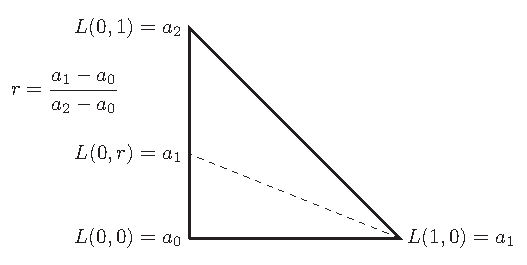
\includegraphics[width=.72\textwidth]{figures/4-10-7.pdf}\\图 4.10.7\end{center}
\textbf{证明：}只需考虑二等分情形 $r=2$。取仿射函数 $L(x,y)=a_0+(a_1-a_0)x+(a_2-a_0)y$，其顶点值如图所示。令 $W=T\circ L$。其三条边分别是 $T_1,T,T_0$，故 $\partial W=T_1-T+T_0$，即 $T$ 同调于 $T_0+T_1$。\translatornote{原书证明末句把这两个分段链误写为 $T_1+T_2$。}\hfill$\square$

\textbf{定理 4.10.15 的证明：}(1) 要证 $\chi([\gamma\cdot\gamma'])=\chi[\gamma]+\chi[\gamma']$。由上一个引理，乘积道路作为奇异单形同调于链 $\gamma+\gamma'$，即得结论。

(2) 假设 $X$ 道路连通。对每个 $x\in X$，选道路 $\zeta_x$ 从 $x_0$ 到 $x$，取 $\zeta_{x_0}$ 为常值道路；其逆向道路为 $\zeta_x^{-1}(t)=\zeta_x(1-t)$。

\sourcepage{256}
给定奇异一维闭链 $z=\sum n_i\sigma_i$，构造闭路
\[
\gamma_i(t)=\begin{cases}
\zeta_{\sigma_i(0)}(3t),&0\le t\le\tfrac13,\\
\sigma_i(3t-1),&\tfrac13\le t\le\tfrac23,\\
\zeta_{\sigma_i(1)}^{-1}(3t-2),&\tfrac23\le t\le1.
\end{cases}
\]
由 (1) 及分段引理，
\[
\chi\left(\prod_i[\gamma_i]^{n_i}\right)
=\sum_i n_i\{\gamma_i\}
=\left\{\sum_i n_i(\zeta_{\sigma_i(0)}-\zeta_{\sigma_i(1)})+z\right\}.
\]
由于 $z$ 闭，$\sum n_i(\sigma_i(1)-\sigma_i(0))=0$。对其中每个端点 $x$，其总系数为零；将同一点换成预先固定的道路 $\zeta_x$，总系数仍为零。因此上式的道路项抵消，结果恰为 $\{z\}$，证明满射。

(3) 记换位子子群为 $C$。因为 $H_1(X)$ 交换，$\chi$ 将每个换位子映为零，故 $C\subset\ker\chi$。商群 $\pi_1/C$ 为交换群，这将允许我们交换并合并各项。

\sourcepage{257}
若 $[\gamma]\in\ker\chi$，则作为奇异链有 $\gamma=\partial(\sum n_i\sigma_i)$，其中 $\sigma_i$ 为二维单形。记
\[
\alpha_{i0}(t)=\sigma_i(1-t,t),\quad\alpha_{i1}(t)=\sigma_i(0,t),\quad\alpha_{i2}(t)=\sigma_i(t,0),
\]
则
\[
\gamma=\sum_i n_i(\alpha_{i0}-\alpha_{i1}+\alpha_{i2}).\tag{$\dagger$}
\]
这是真正的链相等，而不只是同调；合并相同道路后，$\gamma$ 的系数为 $1$，其他道路系数为零。
\begin{center}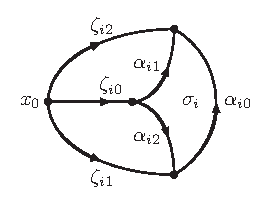
\includegraphics[width=.43\textwidth]{figures/4-10-8.pdf}\\图 4.10.8：单形、各边及从基点到顶点的道路\end{center}
记三个顶点为
\begin{align*}
x_{i0}&=\sigma_i(0,0)=\alpha_{i1}(0)=\alpha_{i2}(0),\\
x_{i1}&=\sigma_i(1,0)=\alpha_{i0}(0)=\alpha_{i2}(1),\\
x_{i2}&=\sigma_i(0,1)=\alpha_{i0}(1)=\alpha_{i1}(1).
\end{align*}
简记 $\zeta_{ij}=\zeta_{x_{ij}}$。将各边补成以 $x_0$ 为基点的闭路：
\[
\beta_{i0}=\zeta_{i1}\cdot\alpha_{i0}\cdot\zeta_{i2}^{-1},\quad
\beta_{i1}=\zeta_{i0}\cdot\alpha_{i1}\cdot\zeta_{i2}^{-1},\quad
\beta_{i2}=\zeta_{i0}\cdot\alpha_{i2}\cdot\zeta_{i1}^{-1}.
\]
道路乘积从左到右依次行走，并适当重参数化为 $[0,1]$ 上的映射，相当于分段引理的逆过程。

\sourcepage{258}
\begin{center}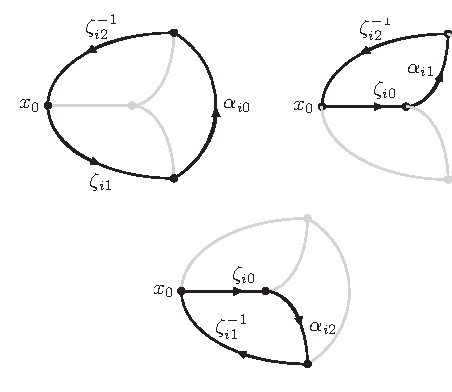
\includegraphics[width=.7\textwidth]{figures/4-10-9.pdf}\\图 4.10.9：三个补成的闭路\end{center}
令 $\beta_i=\beta_{i0}\cdot\beta_{i1}^{-1}\cdot\beta_{i2}$。展开后，成对的道路及其逆可通过保持端点的同伦消去，得
\begin{align*}
\beta_i
&=\zeta_{i1}\cdot\alpha_{i0}\cdot\zeta_{i2}^{-1}\cdot
(\zeta_{i0}\cdot\alpha_{i1}\cdot\zeta_{i2}^{-1})^{-1}\cdot
\zeta_{i0}\cdot\alpha_{i2}\cdot\zeta_{i1}^{-1}\\
&\simeq\zeta_{i1}\cdot\alpha_{i0}\cdot\alpha_{i1}^{-1}\cdot\alpha_{i2}\cdot\zeta_{i1}^{-1}.
\end{align*}
\begin{center}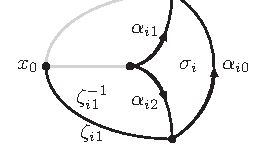
\includegraphics[width=.43\textwidth]{figures/4-10-10.pdf}\\图 4.10.10：闭路 $\beta_i$\end{center}
它从基点走到 $x_{i1}$，绕单形边缘一周，再原路返回。将 $\Delta_2$ 收缩到 $(1,0)$，便将绕边缘的部分收缩到 $x_{i1}$。所以 $\beta_i\simeq\zeta_{i1}\cdot\zeta_{i1}^{-1}\simeq x_0$，即 $[\beta_i]=1$，因而
\[
\prod_i[\beta_i]^{n_i}=1.\tag{$\ddagger$}
\]

\sourcepage{259}
若基本群交换，就可像 ($\dagger$) 那样合并道路项；一般基本群不交换，不能这样做。但在交换商群 $\pi_1/C$ 中可以。记闭路 $\beta$ 的陪集为 $\lceil\beta\rceil$。由 ($\ddagger$)，有 $\prod_i\lceil\beta_i\rceil^{n_i}=1$；而由 ($\dagger$)，把每条边按上述相同规则补成闭路后，所有同一道路的项仍抵消，所得积等于 $\lceil\gamma\rceil$。因此 $\lceil\gamma\rceil=1$，即 $[\gamma]\in C$。这证明 $\ker\chi=C$。

(4) 由 (2)、(3) 立即得到。\hfill$\square$

\begin{center}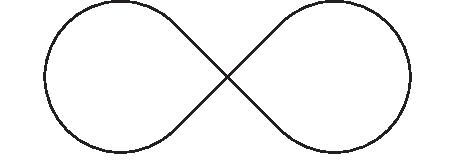
\includegraphics[width=.65\textwidth]{figures/4-10-11.pdf}\\图 4.10.11：数字 8 空间\end{center}
\entry{命题}{4.10.17}图 4.10.11 的数字 8 空间 $X$ 的基本群不是阿贝尔群。

\textbf{证明：}仍把圆周视为复数单位圆，并将 $X$ 视为 $(S^1\times\{1\})\cup(\{1\}\times S^1)$，基点为 $(1,1)$。这个模型位于两个平面的笛卡儿积中：两个圆周只在基点相交。

\sourcepage{260}
令 $\gamma(t)=(e^{2\pi it},1)$、$\eta(t)=(1,e^{2\pi it})$，其逆向闭路分别把 $t$ 换为 $1-t$。令 $\zeta=\gamma\cdot\eta\cdot\gamma^{-1}\cdot\eta^{-1}$。它依次逆时针绕第一、第二圆周，再顺时针绕第一、第二圆周。

反设基本群交换，则 $[\zeta]=1$，存在 $F:I\times I\to X$，使 $F(t,0)=F(0,u)=F(1,u)=(1,1)$，$F(t,1)=\zeta(t)$。定义
\[
\varphi:(\R\times\Z)\cup(\Z\times\R)\to X,\qquad
\varphi(w,z)=(e^{2\pi iw},e^{2\pi iz}).
\]
仿照命题 4.10.8，分别对两坐标作提升，可得 $\zeta'$ 与 $F'$，满足 $\varphi\zeta'=\zeta$、$\varphi F'=F$。由于至少有一个指数坐标为 $1$，提升的像确实在上述整数网格中。$\zeta'$ 正是沿单位正方形边缘逆时针绕一周的闭路。

再定义 $\psi$：从正方形中心 $(1/2,1/2)$ 作射线，经网格点 $(x,y)$，取它与 $\Bd(I\times I)$ 的唯一交点作为 $\psi(x,y)$，见图 4.10.12。它在正方形边缘上为恒等映射。\translatornote{原书用从 $(x,y)$ 到中心的线段与边缘的交点描述此映射；网格点没有落在正方形内部，故该描述给出相同的径向投影。}

于是 $\psi\zeta'$ 绕正方形边缘一周。因该边缘同胚于圆周，命题 4.10.8 说明此闭路不可能同伦于常值闭路；但 $\psi F'$ 恰给出它与常值 $(0,0)$ 的同伦，矛盾。\hfill$\square$

\sourcepage{261}
\begin{center}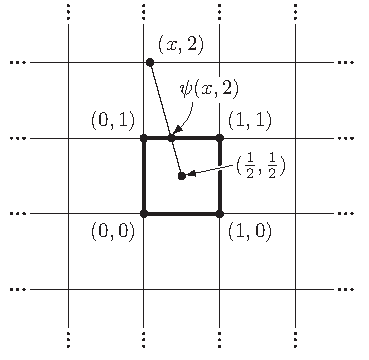
\includegraphics[width=.55\textwidth]{figures/4-10-12.pdf}\\图 4.10.12：映射 $\psi$\end{center}
\subsection*{习题}
\begin{enumerate}
\item 证明定义 4.10.1 的关系具有自反性、对称性。
\item 证明引理 4.10.5 的 (2)、(3)、(4)。
\item 参照命题 4.10.8 的证明，验证 $[\rho_m][\rho_n]=[\rho_{m+n}]$。
\item \begin{enumerate}[label=(\alph*)]
\item 证明 $n\ge2$ 时，$\R^n$ 中每条闭路均同伦于包含在有限条直线之并中的闭路。
\item 证明 $n\ge2$ 时，$S^n$ 中每条闭路均同伦于包含在有限条大圆之并中的闭路。这就验证了例 4.10.10 中的断言。\translatornote{原书将这里引用的例号印为 4.10.9。}
\end{enumerate}
\item 设 $X=U\cup V$，其中 $U,V$ 是单连通开集。若 $U\cap V$ 道路连通，证明 $X$ 单连通。
\end{enumerate}

\section{商空间续论}
\sourcepage{261--262}
第 2.8 节已回顾商空间理论的一些方面，现在进一步讨论，特别考察其分离公理。商空间的分离性质通常表现不好；一般很难保证比 $T_1$ 更强的分离性，甚至 Hausdorff 性也常不易验证。下面给出三种可保证商空间为 Hausdorff 空间、事实上为正规空间的情形。

\entry{定理}{4.11.1}若商映射 $p:X\to Y$ 是闭映射，且 $X$ 正规，则 $Y$ 正规。

\textbf{证明：}因 $X$ 的单点集闭，闭映射将它映为 $Y$ 的闭单点集，故 $Y$ 为 $T_1$ 空间。设 $A,B\subset Y$ 为不交闭集，在 $X$ 中取不交开集 $U,V$，分别包含 $p^{-1}(A),p^{-1}(B)$。像集 $p(U),p(V)$ 不一定开，也不一定不交（图 4.11.1）。改令 $C=X\setminus U$、$D=X\setminus V$，则 $p(C),p(D)$ 闭。
\begin{center}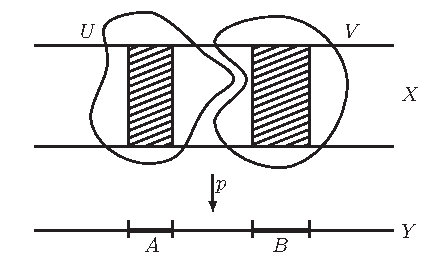
\includegraphics[width=.65\textwidth]{figures/4-11-1.pdf}\\图 4.11.1\end{center}
因为 $U\cap V=\varnothing$，De Morgan 定律给出 $C\cup D=X$，从而 $p(C)\cup p(D)=Y$，于是 $Y\setminus p(C)$ 与 $Y\setminus p(D)$ 不交。又因 $C$ 与 $p^{-1}(A)$ 不交，$p(C)$ 与 $A$ 不交，所以前者包含 $A$；同理后者包含 $B$。这就是所需的不交开邻域。\hfill$\square$

若 $X^*$ 是 $X$ 到闭集的一个分划，且商映射 $p:X\to X^*$ 闭，经典上称之为 $X$ 的\textbf{上半连续分解}（upper semicontinuous decomposition）。具体地，即每个闭集 $A\subset X$ 的\textbf{饱和集} $p^{-1}p(A)$ 都闭。此时 $X$ 正规蕴含 $X^*$ 正规。

\sourcepage{263}
\entry{定义}{4.11.2}设 $X,Y$ 不交，$A\subset X$ 闭，$f:A\to Y$ 连续。先给 $X\cup Y$ 赋拓扑和拓扑，再对每个 $y\in Y$，把 $\{y\}\cup f^{-1}(y)$ 压缩为一点，$X\setminus A$ 中的点保持各自独立。所得商空间记为 $X\cup_fY$，称为由 $f$ 决定的\textbf{粘合空间}（adjunction space），见图 4.11.2。
\begin{center}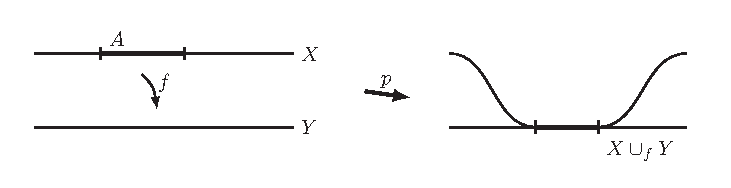
\includegraphics[width=.96\textwidth]{figures/4-11-2.pdf}\\图 4.11.2\end{center}
设商映射为 $p$。它把 $Y$ 同胚地映到商空间的闭子空间：限制 $p|_Y$ 连续且单射；若 $C\subset Y$ 闭，则 $f^{-1}(C)$ 在 $A$ 中闭，因 $A$ 闭而在 $X$ 中闭，所以 $p^{-1}p(C)=C\cup f^{-1}(C)$ 在拓扑和中闭。由商拓扑定义，$p(C)$ 闭。因此 $p|_Y$ 是到闭子空间 $p(Y)$ 的同胚。通常把 $Y$ 与该像认同。

若 $X,Y$ 为 $T_1$ 空间，每个等价类都闭，故 $X\cup_fY$ 也是 $T_1$ 空间。但 $p$ 通常不是闭映射，不能直接应用上一定理得到更强分离性。不过仍有如下结果。

\entry{定理}{4.11.3}若 $X,Y$ 正规，则 $X\cup_fY$ 正规。

\textbf{证明：}设 $B,C$ 为粘合空间中不交闭集，记
\[
B_X=p^{-1}(B)\cap X,\quad C_X=p^{-1}(C)\cap X,\quad
B_Y=p^{-1}(B)\cap Y,\quad C_Y=p^{-1}(C)\cap Y.
\]
\sourcepage{264}
由 Urysohn 引理，可取连续 $g:Y\to[0,1]$，在 $B_Y$ 上为 $0$、在 $C_Y$ 上为 $1$。因此 $gf$ 在 $A\cap B_X$ 上为 $0$、在 $A\cap C_X$ 上为 $1$。在闭集 $A\cup B_X\cup C_X$ 上定义 $h$：在 $A$ 上等于 $gf$，在 $B_X$ 上为 $0$，在 $C_X$ 上为 $1$。各部分定义相容，由闭集粘贴引理连续。再由 Tietze 延拓定理延拓为 $k:X\to[0,1]$。
\begin{center}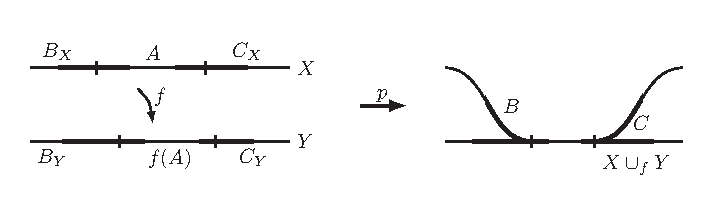
\includegraphics[width=.96\textwidth]{figures/4-11-3.pdf}\\图 4.11.3\end{center}
在拓扑和上定义 $\ell$，使其在 $X$ 上为 $k$、在 $Y$ 上为 $g$。它连续，且在每个等价类上为常值，因为 $k(a)=g(f(a))$。因此诱导商空间上的连续函数，在 $B$ 上为 $0$、在 $C$ 上为 $1$，说明空间正规。\hfill$\square$

我们已定义空间拓扑与子空间族协调的含义。现在稍加推广：给定拓扑空间族 $\{X_\alpha\}$，但其并集 $X$ 尚无拓扑。何时可在 $X$ 上赋予拓扑，使每个 $X_\alpha$ 保持原有子空间拓扑，且 $X$ 与这些子空间协调？

\entry{引理}{4.11.4}设集合 $X=\bigcup X_\alpha$。
\begin{enumerate}[label=(\alph*)]
\item 若已有一个底集为 $X$ 的拓扑空间 $X_T$，使所有 $X_\alpha$ 是其子空间，则可在 $X$ 上赋予与诸 $X_\alpha$ 协调的拓扑，且仍保持各子空间的原拓扑。这个拓扑一般比 $X_T$ 更细。
\item 若每个 $X_\alpha\cap X_\beta$ 在两者中都闭，且从两者继承的拓扑相同，则 $X$ 存在与诸 $X_\alpha$ 协调的拓扑；每个 $X_\alpha$ 在该拓扑中闭。
\end{enumerate}

\sourcepage{265}
\textbf{证明：}(a) 定义 $X_C$ 的闭集为所有满足 $A\cap X_\alpha$ 在 $X_\alpha$ 中闭的集合 $A$。这类集合对任意交及有限并封闭，且含空集和全集，故定义拓扑。若 $A$ 在 $X_T$ 中闭，它与每个子空间相交均闭，故也在 $X_C$ 中闭，因此后者更细。

要证每个 $X_\alpha$ 保持其子空间拓扑，只需比较闭集。一个 $X_C$ 中闭集与 $X_\alpha$ 的交按定义闭。反过来，若 $B\subset X_\alpha$ 闭，因它原是 $X_T$ 的子空间，可写 $B=A\cap X_\alpha$，其中 $A$ 在 $X_T$ 中闭，也在 $X_C$ 中闭。因此两种拓扑相同，协调性随即由定义成立。

(b) 仍用同样规则定义 $X_C$。若 $B$ 在 $X_\alpha$ 中闭，对任意 $\beta$，
\[
B\cap X_\beta=B\cap(X_\alpha\cap X_\beta)
\]
在交空间中闭；因交空间在 $X_\beta$ 中闭且两边继承拓扑相同，它在 $X_\beta$ 中闭。因此 $B$ 本身在 $X_C$ 中闭。\translatornote{原书上述等式右端首个集合误印为 $X$，应为 $B$。}这既说明子空间拓扑不变，也说明各 $X_\alpha$ 闭，完成证明。\hfill$\square$

\entry{例}{4.11.5}若 $K$ 是 $E^J$ 中的复形，则 $|K|$ 先有从 $E^J$ 继承的拓扑，其中每个单形均为子空间。由引理 (a)，还可赋予与所有单形协调的拓扑，它一般更细。这是第 1.3 节直接证明过的事实。

一般而言，即使各 $X_\alpha$ 有良好的分离性质，协调拓扑也未必保留这些性质。但对可数个闭子空间之并，可得如下定理。

\sourcepage{266}
\entry{定理}{4.11.6}若 $X$ 是可数个正规闭子空间 $X_i$ 之并，且拓扑与它们协调，则 $X$ 正规。

\textbf{证明：}每个点 $p$ 的单点集与每个 $X_i$ 相交均闭，故在 $X$ 中闭，$X$ 为 $T_1$ 空间。设 $A,B$ 为不交闭集，令 $Y_0=A\cup B$，$Y_n=X_1\cup\cdots\cup X_n\cup A\cup B$。在 $Y_0$ 上定义连续函数 $f_0$，在 $A$ 上为 $0$、在 $B$ 上为 $1$。

归纳延拓：$Y_n\cap X_{n+1}$ 在正规空间 $X_{n+1}$ 中闭，故用 Tietze 定理将 $f_n$ 在此交集上的限制延拓为 $g:X_{n+1}\to[0,1]$。由于 $Y_n$ 与 $X_{n+1}$ 在 $Y_{n+1}$ 中均闭，$f_n,g$ 可粘贴为连续的 $f_{n+1}$。所有 $f_n$ 合成 $f:X\to[0,1]$，仍在 $A,B$ 上分别为 $0,1$。它在每个 $X_n$ 上连续，由协调拓扑性质在 $X$ 上连续，故 $X$ 正规。\hfill$\square$

\entry{定义}{4.11.7}若空间的拓扑与其所有紧子空间协调，则称该空间\textbf{紧生成}（compactly generated）。这个定义用于习题 3。

\subsection*{习题}
\begin{enumerate}
\item 设 $X=\bigcup X_\alpha$，且每个交集 $X_\alpha\cap X_\beta$ 从两者继承相同拓扑。
\begin{enumerate}[label=(\alph*)]
\item 若所有交集在两边均开，证明 $X$ 上存在使诸 $X_\alpha$ 都成为子空间的拓扑。
\item 证明一般情况下，这样的拓扑未必存在。〔提示：取实数轴中不交稠密集 $A,B$，使其并的补集也稠密。令 $A,B,X_1=\R\setminus A,X_2=\R\setminus B$ 均继承实数轴的拓扑，$X_3=A\cup B$ 则取 $A,B$ 的拓扑和。令 $X=X_1\cup X_2\cup X_3$，考察 $\overline A$。〕
\end{enumerate}
\item 回忆 $\R^\infty=E^J$，其中 $J$ 为正整数集，每个 $\R^n\times\{0\}$ 都是其子空间。证明
\[
f:\R^\infty\to\R,\qquad f(x)=\sum_{i=1}^{\infty}ix_i
\]
在通常的度量拓扑中不连续，但在与诸 $\R^n\times\{0\}$ 协调的拓扑中连续。
\item 设 $X_C$ 为底集 $X$ 上与 $X$ 的所有紧子空间协调的拓扑。
\begin{enumerate}[label=(\alph*)]
\item 证明 $B\subset X$ 在从 $X$ 继承的拓扑中紧，当且仅当在从 $X_C$ 继承的拓扑中紧。〔提示：还要证明这两个子空间拓扑实际上相同。〕
\item 证明 $X_C$ 紧生成，从而 $(X_C)_C=X_C$。
\item 证明恒等包含 $X_C\to X$ 诱导奇异同调同构。
\item 记 $X\times_CY=(X\times Y)_C$。证明对复形 $K,L$，$|K|\times_C|L|$ 的拓扑与所有 $\sigma\times\tau$（$\sigma\in K,\tau\in L$）协调。与第 2.8 节习题 6 比较。〔提示：若 $D\subset X\times Y$ 紧，则 $D\subset A\times B$，其中 $A,B$ 紧。〕
\end{enumerate}
\item 证明定理 4.11.6 不适用于不可数族。〔提示：令 $[0,\omega_1]$ 为带最小元和最大元的不可数良序集，其中每个 $\alpha<\omega_1$ 的初段 $[0,\alpha]$ 可数。空间 $[0,\omega_1)\times[0,\omega_1]$ 不正规，见 [Mun00] 第 203 页例 2。〕
\item 寻找一个附加条件，使定理 4.11.6 对不可数并也成立。
\end{enumerate}

\section{CW 复形}
\sourcepage{267--268}
我们曾说单纯同调的优点之一是可有效计算。但除最简单的情况外，直接计算所需的工作量通常大到无法手算。即使第 1.7 节计算环面、Klein 瓶的同调时，也没有完全直接计算，而是用了颇具针对性的几何论证，把问题化为较简单的计算。

现在将这些方法整理为计算同调群的系统方法，它既适用于单纯同调，也适用于奇异同调。本节引入比单纯复形更一般的 \textbf{CW 复形}，由 J. H. C. Whitehead 在 [Whi49] 中提出。下一节给每个 CW 复形指定一个\textbf{胞腔链复形}，用它计算底空间的同调。这个链复形比奇异或单纯链复形简单得多。最后一节将用此方法计算实射影空间、复射影空间等的同调。

\entry{定义}{4.12.1}同胚于 $B^m$ 的空间称为 $m$ 维\textbf{胞腔}；同胚于 $\Int B^m$ 的空间称为 $m$ 维\textbf{开胞腔}（open cell）。两种情况下，维数 $m$ 均由空间唯一确定。\translatornote{原书开胞腔定义中的球维数误印为 $n$，应为 $m$。}

\entry{定义}{4.12.2}\textbf{CW 复形}由空间 $X$ 及一族两两不交、并为 $X$ 的开胞腔 $e_\alpha$ 组成，满足：
\begin{enumerate}[label=(\arabic*)]
\item $X$ 为 Hausdorff 空间。
\item 对每个 $m$ 维开胞腔，有连续映射 $f_\alpha:B^m\to X$，把 $\Int B^m$ 同胚地映到 $e_\alpha$，并把 $\Bd B^m$ 映入有限个维数小于 $m$ 的开胞腔之并。
\item 若 $A\cap\overline e_\alpha$ 对每个 $\alpha$ 都在 $\overline e_\alpha$ 中闭，则 $A$ 在 $X$ 中闭。
\end{enumerate}
Whitehead 称 (2) 的有限性为\textbf{闭包有限性}（closure-finiteness）；(3) 表示 $X$ 具有相对于胞腔闭包族的\textbf{弱拓扑}（weak topology）。这两个词就是 CW 中字母 C、W 的来源。

通常记 $\dot e_\alpha=\overline e_\alpha\setminus e_\alpha$。条件 (1)、(2) 蕴含 $f_\alpha(B^m)=\overline e_\alpha$，且 $f_\alpha(\Bd B^m)=\dot e_\alpha$。事实上，由连续性，闭球的像包含于开球像的闭包；另一方面，闭球像紧，在 Hausdorff 空间中闭，并包含 $e_\alpha$，故等于其闭包。边界像与 $e_\alpha$ 不交，因此恰为 $\dot e_\alpha$。

条件 (3) 的逆命题显然成立。映射 $f_\alpha$ 称为胞腔的\textbf{特征映射}（characteristic map）。定义只指定空间及开胞腔族，并不唯一指定特征映射。我们习惯用 $X$ 同时表示 CW 复形及其底空间。

\sourcepage{269}
若开胞腔仅有有限个，称为\textbf{有限 CW 复形}。此时 (2) 的有限性自动成立，(3) 也由其余条件推出：若每个 $A\cap\overline e_\alpha$ 在胞腔闭包中闭，则它在 $X$ 中也闭，有限并 $A$ 因而闭。

有限 CW 复形当然紧。反过来，CW 复形的任意紧子集只能与有限个开胞腔相交；证明留作习题，其中需要闭包有限性。

下面的引理直接来自第 2.8 节关于协调拓扑的一般结果。

\entry{引理}{4.12.3}映射 $f:X\to Y$ 连续，当且仅当每个限制 $f|_{\overline e_\alpha}$ 连续。映射 $F:X\times I\to Y$ 连续，当且仅当每个 $F|_{\overline e_\alpha\times I}$ 连续。

\entry{例}{4.12.4}将环面视为矩形的通常商空间（图 4.12.1）。它有一个二维开胞腔，即矩形内部的像；两个一维开胞腔，即开边的像；一个零维胞腔，即顶点的像。三个定义条件立即成立。
\begin{center}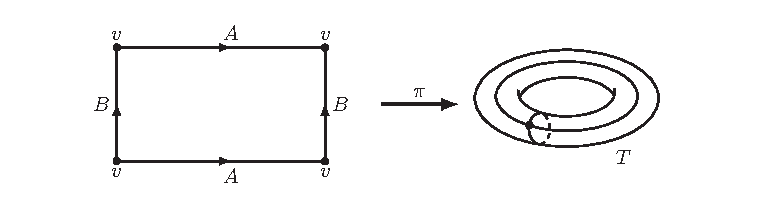
\includegraphics[width=.96\textwidth]{figures/4-12-1.pdf}\\图 4.12.1\end{center}
同样，Klein 瓶也可取各维相同数目的胞腔。实射影平面可取零、一、二维各一个胞腔。更一般地，第 1.7 节习题中的 $n$ 重环面连通和有一个二维胞腔、一个零维胞腔和 $2n$ 个一维胞腔；$n$ 重实射影平面连通和则有一个二维胞腔、一个零维胞腔和 $n$ 个一维胞腔。$k$ 重愚人帽也可取零、一、二维各一个胞腔。

\sourcepage{270}
\entry{例}{4.12.5}将 $B^n$ 的边界压缩为一点所得商空间同胚于 $S^n$，证明留给读者。因此球面可取一个 $n$ 维开胞腔和一个零维胞腔，不需要其他胞腔，见图 4.12.2。
\begin{center}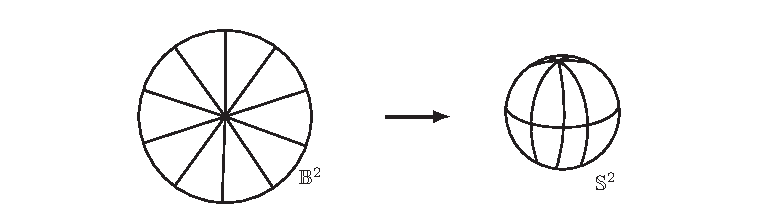
\includegraphics[width=.96\textwidth]{figures/4-12-2.pdf}\\图 4.12.2\end{center}

\entry{例}{4.12.6}条件 (2) 并不要求 $\dot e_\alpha$ 本身等于若干低维开胞腔之并。例如图 4.12.3 的空间在零、一、二维各有一个胞腔，但二维胞腔的边界只包含于低维胞腔之并，并不等于它。
\begin{center}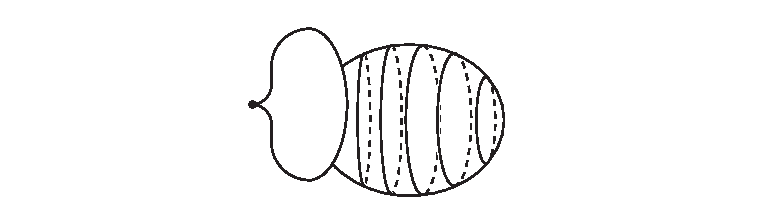
\includegraphics[width=.96\textwidth]{figures/4-12-3.pdf}\\图 4.12.3\end{center}

\entry{例}{4.12.7}设 $K,L$ 为单纯复形，且 $K$ 局部有限。空间 $|K|\times|L|$ 可取 $(\Int\sigma)\times(\Int\tau)$ 为开胞腔，其中 $\sigma\in K,\tau\in L$。特征映射可取为 $B^m\to\sigma\times\tau$ 的同胚，而且每个闭胞腔的边界是低维开胞腔的有限并。条件 (3) 来自第 2.8 节习题 6，其中用到了 $K$ 的局部有限性。

\sourcepage{271}
\entry{定义}{4.12.8}若 CW 复形的特征映射可取为同胚，且每个 $\dot e_\alpha$ 都等于有限个开胞腔之并，则称为\textbf{正则胞腔复形}（regular cell complex）。这种复形总能三角剖分，使每个闭胞腔是某个子复形的多面体；证明与引理 2.7.3 中对 $|K|\times I$ 的证明类似。

\entry{例}{4.12.9}许多从旧空间构造新空间的方法会保留 CW 结构。例如，两个 CW 复形的乘积 $X\times Y$ 在 $Y$ 局部紧时仍为 CW 复形。粘合空间也常如此：若 $A$ 是 $X$ 的子复形，且 $f:A\to Y$ 把每个 $p$ 维胞腔映入 $Y$ 中维数至多为 $p$ 的开胞腔之并，则称 $f$ 为\textbf{胞腔映射}（cellular map）。此时可证 $X\cup_fY$ 为 CW 复形。

\entry{定义}{4.12.10}设 $Y\subset X$ 为若干开胞腔之并，且每个包含于 $Y$ 的开胞腔，其闭包也包含于 $Y$。下面将证明 $Y$ 在 $X$ 中闭，并且自身构成 CW 复形，称为 $X$ 的\textbf{子复形}。特别地，所有维数至多为 $p$ 的开胞腔之并 $X^p$ 满足这些条件，称为 $X$ 的\textbf{$p$ 维骨架}（$p$-skeleton）。

先验证 $Y$ 的 CW 条件。Hausdorff 性显然；其胞腔的特征映射把整个闭球映入 $Y$，且边界像所碰到的有限个低维胞腔也在 $Y$ 内。只需验证弱拓扑。

设 $B\subset Y$，且 $B\cap\overline e_\alpha$ 对每个在 $Y$ 中的胞腔闭。若 $e_\beta$ 不在 $Y$ 中，则 $Y\cap\overline e_\beta\subset\dot e_\beta$，并包含于有限个在 $Y$ 中的开胞腔 $e_1,\ldots,e_k$ 之并。因此
\[
B\cap\overline e_\beta=\left[\bigcup_{i=1}^k(B\cap\overline e_i)\right]\cap\overline e_\beta.
\]
每个 $B\cap\overline e_i$ 在 $X$ 中闭，故右端闭。由 $X$ 的弱拓扑，$B$ 在 $X$ 中闭，特别在 $Y$ 中闭。因此 $Y$ 具有所需弱拓扑。取 $B=Y$ 还说明 $Y$ 自身在 $X$ 中闭。

\sourcepage{272}
闭包有限性在此证明中至关重要。

\entry{例}{4.12.11}设 $X$ 是平面中的二维单形，取通常拓扑，分解为一个二维开胞腔与边界上无穷多个零、一维胞腔，如图 4.12.4。除条件 (2) 的有限性外，其余条件均成立；条件 (3) 因二维胞腔的闭包等于整个 $X$ 而自动成立。若给边界胞腔之并 $Y$ 赋以相对于各闭胞腔的弱拓扑，$Y$ 自身是 CW 复形，但不具有 $X$ 的子空间拓扑：后者是紧的单形边界，前者却不紧。
\begin{center}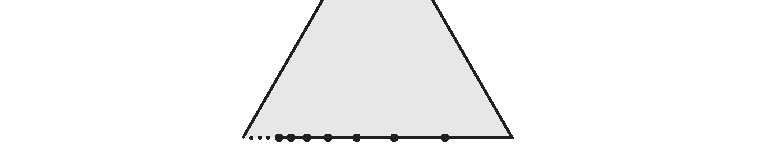
\includegraphics[width=.96\textwidth]{figures/4-12-4.pdf}\\图 4.12.4\end{center}

\entry{定义}{4.12.12}若 CW 复形 $X$ 有三角剖分 $h:|K|\to X$，使每个骨架 $X^p$ 都由维数至多为 $p$ 的子复形三角剖分，则称 $X$ 为\textbf{可三角剖分的 CW 复形}。\footnote{维数条件实际上是多余的，见习题 2。}

前述各例均可三角剖分。下面给出一个不能的例子，证明要用第 4.8 节的局部同调。

\entry{例}{4.12.13}在 $\R^3$ 中，令 $A$ 为正方形与三角形之并，三角形的一条边恰为正方形的对角线 $D$。它是三个三角形共用一条边组成的复形的多面体。在正方形中画一条摆动的弧 $C$，使它与 $D$ 交于一个无限且全不连通的集合，例如 $x\sin(1/x)$ 型曲线。把三维球沿映射 $f:S^2\to C$ 粘到 $A$，其中每条从南极到北极的大圆弧均同胚地映到 $C$，见图 4.12.5。

\sourcepage{273}
\begin{center}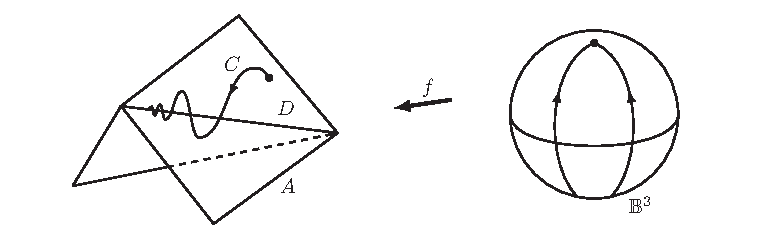
\includegraphics[width=.96\textwidth]{figures/4-12-5.pdf}\\图 4.12.5\end{center}
所得 $X$ 是 CW 复形：取 $A$ 的开单形为低维胞腔，球内部为唯一三维开胞腔 $e^3$。但底空间本身不能三角剖分。

反设 $h:|K|\to X$ 为三角剖分。将 $X$ 写成不交并 $(A\setminus C)\cup C\cup e^3$。若 $x\in e^3$，则它有开三维球邻域，故 $H_3(X,X\setminus\{x\})\cong\Z$；若 $x\in A\setminus C$，有邻域完全包含于二维复形 $A$，故此群由定理 4.8.14 为零。由引理 4.8.10，任一 $h(\Int\sigma)$ 不能同时碰到这两部分。因此每个闭单形的像或包含于 $A$，或包含于 $\overline e^3$。于是 $A,\overline e^3$ 及其交 $C$ 都由 $h$ 三角剖分。

再看 $A$ 自身的局部同调。对角线 $D$ 的内部点 $x$ 满足 $H_2(A,A\setminus\{x\})\cong\Z\oplus\Z$：$A$ 可视为以 $x$ 为顶点、底空间同胚于字母 $\theta$ 形曲线的锥，故由长正合列此群同构于 $H_1(\theta)$。而 $D$ 外的点，局部二维同调或为 $\Z$（三角形内部），或为零。再次由引理 4.8.10，若单形内部像碰到 $\Int D$，便完全包含于 $D$。因此 $D$ 也由 $h$ 三角剖分，进而 $C\cap D$ 亦然。

但 $X$ 紧，所以 $K$ 必为有限复形；其子复形不可能具有无限多个连通分支，而 $C\cap D$ 恰有无限多个分支，矛盾。

把 CW 复形看作由闭球通过商空间粘成，往往很有帮助；也可按这种方式构造新空间，如上例。下面两个定理描述这一过程。CW 复形的\textbf{维数}是胞腔维数的最大值；若无最大值，则称其为无限维。

\sourcepage{274}
\entry{定理}{4.12.14}
\begin{enumerate}[label=(\alph*)]
\item 若 $X$ 为 $p$ 维 CW 复形，则它同胚于把一族闭 $p$ 维球的拓扑和 $\coprod B_\alpha$ 沿连续映射 $g:\coprod\Bd B_\alpha\to X^{p-1}$ 粘到骨架所得的空间。因此 $X$ 正规。
\item 反过来，若 $Y$ 是维数至多为 $p-1$ 的 CW 复形，$g:\coprod\Bd B_\alpha\to Y$ 连续，则将这些闭 $p$ 维球粘到 $Y$ 所得的空间 $X$ 为 CW 复形，$Y$ 为其 $(p-1)$ 维骨架。
\end{enumerate}
\textbf{证明：}(a) 对每个 $p$ 维胞腔取特征映射 $f_\alpha:B^p\to\overline e_\alpha$，令 $B_\alpha=B^p\times\{\alpha\}$。在拓扑和 $E=X^{p-1}\amalg(\coprod B_\alpha)$ 上定义 $\pi:E\to X$：骨架上为包含映射，球上为投影后接 $f_\alpha$。它连续满射，只需证明为商映射。

若 $\pi^{-1}(C)$ 在 $E$ 中闭，则 $C\cap X^{p-1}$ 闭，故与每个低维胞腔闭包的交闭。又对 $p$ 维胞腔，$\pi^{-1}(C)\cap B_\alpha$ 为紧集，其像为 $C\cap\overline e_\alpha$，故在 Hausdorff 空间 $X$ 中闭。由弱拓扑，$C$ 闭，所以 $\pi$ 为商映射。正规性由定理 4.11.3 对 $p$ 归纳得到。

(b) 设 $f:Y\amalg(\coprod B_\alpha)\to X$ 为给定商映射。由 (a)，$Y$ 正规，球的拓扑和也正规，所以定理 4.11.3 说明 $X$ 正规，特别是 Hausdorff。将 $Y$ 认同于其闭像，$f$ 在 $Y$ 上为包含，在球的边界上为 $g$。

取 $Y$ 的原有胞腔及 $e_\alpha=f(\Int B_\alpha)$ 为开胞腔。球内部在拓扑和中开且饱和，限制映射为一一对应的商映射，故为同胚。边界像是 $Y$ 中的紧集，只碰到有限个开胞腔，且这些胞腔维数均小于 $p$，因此条件 (2) 成立。

\sourcepage{275}
最后验证 (3)。若 $C\cap\overline e_\alpha$ 对每个胞腔闭，则 $C\cap Y$ 由 $Y$ 的弱拓扑而闭。对于每个球，
\[
f^{-1}(C)\cap B_\alpha=f^{-1}(C\cap\overline e_\alpha)\cap B_\alpha
\]
闭，因为 $f(B_\alpha)=\overline e_\alpha$，且限制映射连续。因此 $f^{-1}(C)$ 在拓扑和中闭，故 $C$ 在商空间中闭。\hfill$\square$

\entry{定理}{4.12.15}
\begin{enumerate}[label=(\alph*)]
\item 若 $X$ 为 CW 复形，则每个 $X^p$ 在 $X^{p+1}$ 中闭，且 $X$ 是递增骨架族的协调并。因此 $X$ 正规。
\item 反过来，若每个 $X^p$ 为 CW 复形，并为 $X^{p+1}$ 的 $p$ 维骨架，则它们的协调并 $X$ 为 CW 复形，其 $p$ 维骨架恰为 $X^p$。
\end{enumerate}
\textbf{证明：}(a) 若 $C\cap X^p$ 对每个 $p$ 闭，则它与维数至多为 $p$ 的每个胞腔闭包的交都闭。因 $p$ 任意，由弱拓扑 $C$ 闭，故 $X$ 与骨架族协调。各骨架正规，由定理 4.11.6，$X$ 正规。

(b) 若 $p<q$，$X^p\cap X^q=X^p$ 是两者的闭子空间。由引理 4.11.4(b)，协调拓扑存在，各骨架在 $X$ 中闭。每个骨架由上一定理正规，再由定理 4.11.6，$X$ 正规且 Hausdorff。条件 (2) 显然。若 $C$ 与每个胞腔闭包的交闭，则因每个骨架是 CW 复形，$C\cap X^p$ 闭；再由协调拓扑，$C$ 闭。\hfill$\square$

\sourcepage{276}
有时从已有空间出发寻找 CW 结构，如例 4.12.4--4.12.6；有时通过粘合球来构造新空间，如例 4.12.13。以上两个定理给出一般构造，它大大扩展了代数拓扑能有效研究的空间范围。

\subsection*{习题}
\begin{enumerate}
\item 设 $A$ 是 CW 复形 $X$ 的紧子集。
\begin{enumerate}[label=(\alph*)]
\item 证明 $A$ 只与有限个开胞腔相交。证明何处使用了闭包有限性？
\item 证明 $A$ 包含于某个有限子复形。
\end{enumerate}
\item 设三角剖分 $h:|K|\to X$ 在每个骨架上都诱导三角剖分。
\begin{enumerate}[label=(\alph*)]
\item 证明它也在每个胞腔闭包 $\overline e_\alpha$ 上诱导三角剖分。
\item 若 $K_p$ 是剖分 $X^p$ 的子复形，证明其维数至多为 $p$。〔提示：用局部同调群。〕
\end{enumerate}
\item 证明 CW 复形的拓扑紧生成，见第 4.11 节习题 3。
\item 设 $X,Y$ 为 CW 复形，以 $e_\alpha\times e_\beta$ 为乘积的开胞腔。
\begin{enumerate}[label=(\alph*)]
\item 若 $Y$ 局部紧，证明 $X\times Y$ 为 CW 复形。
\item 一般情况下，证明 $X\times_CY$ 为 CW 复形，见第 4.11 节习题 3。
\end{enumerate}
\item 验证正则胞腔复形可三角剖分，使每个闭胞腔是子复形的多面体。
\item 证明 $n$ 维环面为 CW 复形。
\item 证明三维空间中的实心环面为 CW 复形。
\end{enumerate}

\section{CW 复形的同调}
\sourcepage{276--277}
现在说明怎样计算 CW 复形的奇异同调。本节始终以 $X$ 表示 CW 复形，开胞腔为 $e_\alpha$，特征映射为 $f_\alpha$。通常 $H_p$ 表示奇异同调；若 $X$ 可三角剖分，也可理解为单纯同调，因为两者之间有自然同构。

\entry{定义}{4.13.1}令 $D_p(X)=H_p(X^p,X^{p-1})$，并定义 $\partial:D_p(X)\to D_{p-1}(X)$ 为复合
\[
H_p(X^p,X^{p-1})\xrightarrow{\partial_*}H_{p-1}(X^{p-1})\xrightarrow{j_*}H_{p-1}(X^{p-1},X^{p-2}),
\]
其中 $j$ 为包含映射。因为 $H_{p-1}(X^{p-1})\xrightarrow{j_*}H_{p-1}(X^{p-1},X^{p-2})\xrightarrow{\partial_*}H_{p-2}(X^{p-2})$ 正合，所以 $\partial^2=0$。所得链复形 $\mathcal D(X)=\{D_p(X),\partial\}$ 称为 $X$ 的\textbf{胞腔链复形}。

\entry{例}{4.13.2}若 $X=|K|$，开胞腔取开单形，并用单纯同调计算，则 $C_i(K^{(p)},K^{(p-1)})$ 在 $i\ne p$ 时为零，在 $i=p$ 时等于 $C_p(K)$。因此 $H_p(X^p,X^{p-1})=C_p(K)$。胞腔边缘算子也正是单纯边缘算子。所以至少在这种情形，胞腔链复形确实计算 $X$ 的同调。

我们的目标是证明一般情形也类似：$D_p(X)$ 是以有向 $p$ 维胞腔为基的自由阿贝尔群，而且 $\mathcal D(X)$ 的同调同构于 $X$ 的奇异同调。先证明一系列引理。

\entry{引理}{4.13.3}任一 $p$ 维胞腔的特征映射 $f_\alpha:(B^p,S^{p-1})\to(\overline e_\alpha,\dot e_\alpha)$ 都诱导相对同调同构。

\sourcepage{278}
\textbf{证明：}零维时显然。设 $p>0$，记 $\widehat e_\alpha=f_\alpha(0)$。特征映射是商映射，其在饱和开集 $B^p\setminus\{0\}$ 上的限制仍为商映射。径向形变收缩将穿孔球收缩到 $S^{p-1}$，通过商映射 $f'_\alpha\times i_I$ 诱导 $\overline e_\alpha\setminus\{\widehat e_\alpha\}$ 到 $\dot e_\alpha$ 的形变收缩，见图 4.13.1。
\begin{center}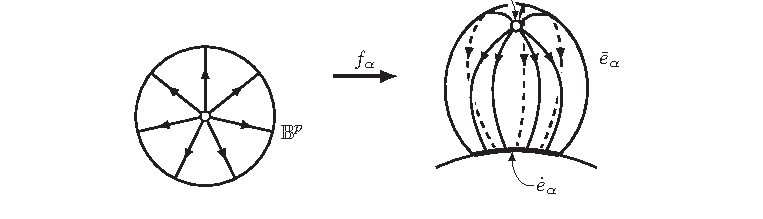
\includegraphics[width=.96\textwidth]{figures/4-13-1.pdf}\\图 4.13.1\end{center}
考虑下列交换图的两行空间偶，以及各列的特征映射：
\[
\begin{split}
(B^p,S^{p-1})\longrightarrow(B^p,B^p\setminus\{0\})
\longleftarrow(\Int B^p,\Int B^p\setminus\{0\}),\\
(\overline e_\alpha,\dot e_\alpha)\longrightarrow
(\overline e_\alpha,\overline e_\alpha\setminus\{\widehat e_\alpha\})
\longleftarrow(e_\alpha,e_\alpha\setminus\{\widehat e_\alpha\}).
\end{split}
\]
左侧两包含映射由形变收缩及定理 4.3.9 诱导同构；右侧两包含映射由切除分别删去 $S^{p-1}$ 和 $\dot e_\alpha$，也诱导同构。最右竖直映射是将 $0$ 映到 $\widehat e_\alpha$ 的同胚，所以最左竖直映射也诱导同构。\hfill$\square$

\entry{引理}{4.13.4}设 $f:X^{p-1}\amalg\coprod B_\alpha\to X^p$ 将骨架表示为由闭 $p$ 维球粘合而成的空间，$S_\alpha=\Bd B_\alpha$。则 $f$ 诱导
\[
H_i(\coprod B_\alpha,\coprod S_\alpha)\cong H_i(X^p,X^{p-1}).
\]

\sourcepage{279}
\textbf{证明：}与上一个引理类似。令 $0_\alpha$ 为各球中心，$\widehat e_\alpha=f(0_\alpha)$。商映射在删去所有球心后的饱和开集上的限制仍为商映射。该定义域可形变收缩到 $X^{p-1}\amalg\coprod S_\alpha$，并通过商映射诱导 $X^p\setminus\bigcup\{\widehat e_\alpha\}$ 到 $X^{p-1}$ 的形变收缩。考虑两行
\[
\begin{split}
(\coprod B_\alpha,\coprod S_\alpha)\to
(\coprod B_\alpha,\coprod(B_\alpha\setminus\{0_\alpha\}))\\
\longleftarrow(\coprod\Int B_\alpha,\coprod(\Int B_\alpha\setminus\{0_\alpha\})),\\[3pt]
(X^p,X^{p-1})\to(X^p,X^p\setminus\bigcup\{\widehat e_\alpha\})
\longleftarrow(\bigcup e_\alpha,\bigcup(e_\alpha\setminus\{\widehat e_\alpha\})).
\end{split}
\]
各列为 $f$。右列为一一对应的商映射，故为同胚；各横向包含映射由形变收缩或切除诱导同构，如上一证明，故得结论。\hfill$\square$

\entry{定理}{4.13.5}群 $H_i(X^p,X^{p-1})$ 在 $i\ne p$ 时为零，在 $i=p$ 时为自由阿贝尔群。若 $\gamma$ 生成 $H_p(B^p,S^{p-1})$，则各 $p$ 维胞腔的一组特征映射给出的 $(f_\alpha)_*\gamma$ 构成一组基。\translatornote{原书生成元所在群误印为 $H_p(B^p,S^p)$，球的边界应为 $S^{p-1}$。}

\textbf{证明：}由上一个引理，所求群同构于 $H_i(\coprod B_\alpha,\coprod S_\alpha)$。每个球在拓扑和中开且彼此不交，所以此群为 $\bigoplus_\alpha H_i(B_\alpha,S_\alpha)$。应用球的相对同调计算即得结论。\hfill$\square$

\entry{定义}{4.13.6}对三元组 $X\supset A\supset B$，短正合列
\[
0\to S_p(A)/S_p(B)\to S_p(X)/S_p(B)\to S_p(X)/S_p(A)\to0
\]
诱导\textbf{三元组的同调正合列}
\[
\cdots\to H_p(A,B)\to H_p(X,B)\to H_p(X,A)\to H_{p-1}(A,B)\to\cdots.
\]
其存在性是定理 3.3.8 的内容，也可由同调公理推出（第 3.5 节习题）。连续映射 $f:(X,A,B)\to(Y,C,D)$ 自然诱导两条正合列间的同态。

\sourcepage{280}
对 $(X,A,B)=(X^p,X^{p-1},X^{p-2})$，这个正合列中的连接同态恰为胞腔边缘算子。因为连接同态与包含映射 $j_*$ 可交换，它等于 $H_p(X^p,X^{p-1})\to H_{p-1}(X^{p-1})\to H_{p-1}(X^{p-1},X^{p-2})$。

为了以后使用，将证明一个稍一般的结果：空间写为递增子空间之并，以 $H_p(X_p,X_{p-1})$ 为链群、三元组的连接同态为边缘。在适当条件下，该链复形计算空间同调。

\entry{定义}{4.13.7}空间 $X$ 的\textbf{滤过}（filtration）是并为 $X$ 的递增子空间列 $X_0\subset X_1\subset\cdots$。空间连同滤过称为\textbf{滤过空间}。若连续映射 $f:X\to Y$ 满足 $f(X_p)\subset Y_p$，称其\textbf{保持滤过}。

\entry{定理}{4.13.8}设 $X$ 有上述滤过，$i<0$ 时令 $X_i=\varnothing$。假设 $H_i(X_p,X_{p-1})=0$（$i\ne p$），且每个紧子集包含于某个 $X_n$。令 $D_p(X)=H_p(X_p,X_{p-1})$，边缘由三元组连接同态定义，则有同构
\[
\lambda:H_p(\mathcal D(X))\to H_p(X),
\]
且对保持滤过的连续映射诱导的同态具有自然性。

\textbf{证明：}先看例 4.13.2 的单纯复形情形，$X_p$ 是 $p$ 维骨架，$\mathcal D(X)=\mathcal C(K)$。由于定义 $H_p(K)$ 只用到 $p+1,p,p-1$ 维链，亦有 $H_p(X)=H_p(K^{(p+1)},K^{(p-2)})$。下面先建立相应的一般结论。

\sourcepage{281}
\textbf{步骤 1。}证明包含映射诱导 $i_*:H_p(X_{p+1})\to H_p(X)$ 为同构。由正合列
\[
\begin{split}
H_{p+1}(X_{p+i+1},X_{p+i})\to H_p(X_{p+i})\to H_p(X_{p+i+1})\\
\to H_p(X_{p+i+1},X_{p+i}),
\end{split}
\]
在 $i\ge1$ 时两端为零，所以从 $X_{p+1}$ 开始，各后续骨架的 $p$ 维同调之间都是同构。

由紧支集性质，每个 $\beta\in H_p(X)$ 来自某个紧子集 $C$ 的同调，而 $C\subset X_{p+k}$，可取 $k\ge1$。于是 $\beta$ 来自 $H_p(X_{p+k})$，再由前述同构来自 $H_p(X_{p+1})$，证明满射。

若 $\beta\in H_p(X_{p+1})$ 在 $X$ 中变为零，则其代表链及使它成为边缘的有限奇异链具有紧载体，包含于某个 $X_{p+k}$。因此 $\beta$ 在 $H_p(X_{p+k})$ 中已为零；因前述映射为同构，$\beta=0$。这证明单射。

\textbf{步骤 2。}证明 $j_*:H_p(X_{p+1})\to H_p(X_{p+1},X_{p-2})$ 为同构。逐步加入相对子空间，考虑三元组正合列
\[
\begin{split}
H_p(X_i,X_{i-1})\to H_p(X_{p+1},X_{i-1})\to H_p(X_{p+1},X_i)\\
\to H_{p-1}(X_i,X_{i-1}).
\end{split}
\]
对 $i\le p-2$，两端均为零，故中间映射为同构。从空集依次加到 $X_{p-2}$ 即得结论。

\sourcepage{282}
\textbf{步骤 3。}对四元组 $X\supset A\supset B\supset C$，可把四个三元组正合列排成下图。取特殊情形 $(X,A,B,C)=(X_{p+1},X_p,X_{p-1},X_{p-2})$，则图中两个上角的群由假设为零。
\begin{center}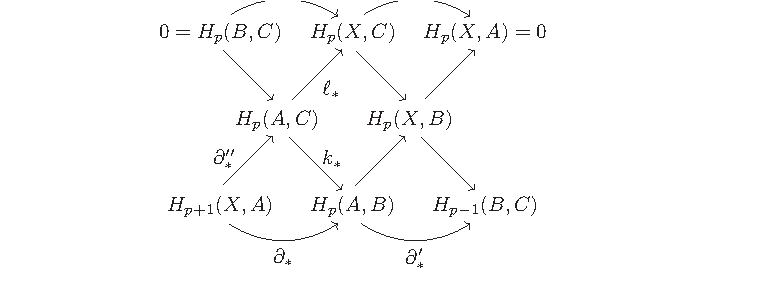
\includegraphics[width=.96\textwidth]{figures/4-13-diagram.pdf}\end{center}
映射 $k_*$ 将 $H_p(A,C)$ 同构地映到 $\ker\partial'_* $；$\ell_*$ 满射，所以 $\ell_*k_*^{-1}$ 将该核满射到 $H_p(X,C)$。由 $\ker\ell_*=\operatorname{im}\partial''_*$ 及图的交换性，其核恰为 $\operatorname{im}\partial_*$。因此
\[
\frac{\ker\partial'_*}{\operatorname{im}\partial_*}\cong H_p(X,C)=H_p(X_{p+1},X_{p-2}).
\]
更一般的图论证见第 3.5 节习题 1。结合前两步，
\[
H_p(X)\cong H_p(X_{p+1})\cong H_p(X_{p+1},X_{p-2})\cong H_p(\mathcal D(X)).
\]
若 $f$ 保持滤过，前两个同构显然与 $f_*$ 可交换，且 $f_*$ 将上述正合图映到 $Y$ 的相应图，故第三个同构也可交换。这证明自然性。\hfill$\square$

\sourcepage{283}
\entry{定理}{4.13.9}设滤过空间 $X=|K|$，每个 $X_p$ 为维数至多为 $p$ 的子复形的多面体，以单纯同调计算，并假定非对角相对同调均为零。则 $H_p(X_p,X_{p-1})$ 可视为 $C_p(K)$ 的子群，且上一定理的 $\lambda$ 由包含映射诱导。具体地，此子群是由 $X_p$ 承载、边缘由 $X_{p-1}$ 承载的所有 $p$ 维链。

\textbf{证明：}每个紧集在有限子复形中，而有限多个单形最终均包含于某个滤过阶段，故上一定理的紧集假设满足。$X_p$ 无 $(p+1)$ 维单形，所以相对 $p$ 维同调就是相对闭链群；$X_{p-1}$ 无 $p$ 维单形，所以 $C_p(X_{p-1})=0$。因此相对闭链恰是上述子群。

上一定理中，$\lambda$ 是将 $\ker\partial'_*$ 的元素沿 $k_*^{-1}$、$\ell_*$、$j_*^{-1}$、$i_*$ 依次映到 $H_p(X)$。这些同态均由包含映射诱导，故在此单纯链解释下，$\lambda$ 正是包含诱导的同态。\hfill$\square$

对每个 $p$ 维胞腔，群 $H_p(\overline e_\alpha,\dot e_\alpha)$ 为无限循环群，其两个生成元称为胞腔的两个\textbf{定向}。开胞腔连同一个定向称为\textbf{有向胞腔}。为每个 $p$ 维胞腔选择定向，再由包含映射送入 $H_p(X^p,X^{p-1})$，就得到胞腔链群的一组基。胞腔链复形的同调由上述定理同构于空间的奇异同调。

\sourcepage{284}
若 $X$ 可三角剖分，则每个胞腔闭包也是子复形的多面体。群 $H_p(\overline e_\alpha,\dot e_\alpha)$ 是由该闭包承载、边缘由 $\dot e_\alpha$ 承载的 $p$ 维单纯链群。它的任一个生成元称为这个空间偶的\textbf{基本闭链}（fundamental cycle）。胞腔链群的每个元素均可唯一写成有限个这样的基本闭链的整数线性组合。

\entry{例}{4.13.10}设 $X$ 是由矩形 $L$ 通常粘合得到的环面或 Klein 瓶。它有一个二维胞腔 $e_2$、两个一维胞腔 $e_1,e'_1$、一个零维胞腔。于是 $D_2\cong\Z$、$D_1\cong\Z\oplus\Z$、$D_0\cong\Z$。
\begin{center}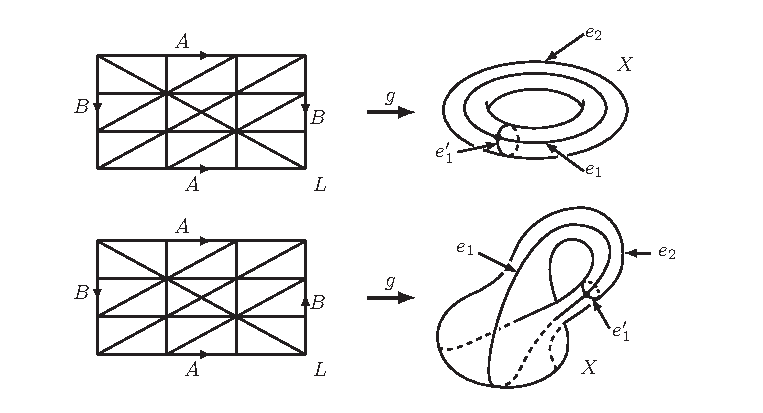
\includegraphics[width=.96\textwidth]{figures/4-13-2.pdf}\\图 4.13.2\end{center}
矩形中所有逆时针定向的二维单形之和 $d$ 是 $(L,\Bd L)$ 的相对闭链，且不是其他闭链的非平凡整数倍，所以为基本闭链。由引理 4.13.3，$\gamma=g_\#d$ 是二维胞腔的基本闭链。

\sourcepage{285}
令 $c_1,c_2,c_3,c_4$ 为图 4.13.3 中按箭头定向的边链。取 $w_1=g_\#c_1$、$z_1=g_\#c_2$ 为两个一维胞腔的基本闭链。计算
\[
\partial c_1=v_4-v_1,\qquad\partial c_2=v_2-v_1,\qquad
\partial d=-c_1+c_2+c_3-c_4.
\]
\begin{center}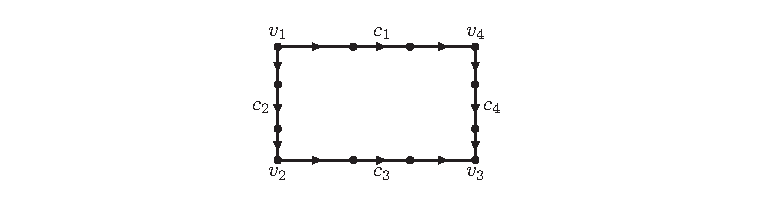
\includegraphics[width=.96\textwidth]{figures/4-13-3.pdf}\\图 4.13.3\end{center}
两种空间均有 $\partial w_1=\partial z_1=0$。环面中，$g_\#c_1=g_\#c_3$、$g_\#c_2=g_\#c_4$，故 $\partial\gamma=0$。Klein 瓶中，第一等式不变，而 $g_\#c_2=-g_\#c_4$，故 $\partial\gamma=2z_1$。因此环面的同调为
\[
H_2\cong\Z,\qquad H_1\cong\Z\oplus\Z,\qquad H_0\cong\Z;
\]
Klein 瓶的同调为
\[
H_2=0,\qquad H_1\cong\Z\oplus\Z/2,\qquad H_0\cong\Z.
\]
这些计算以前做过；现在它们的依据是 CW 复形的一般定理，而不再是第 1.7 节中专门针对这些空间的论证。这正是胞腔理论使计算系统化的意义。

\sourcepage{286}
\entry{例}{4.13.11}设 $n>1$。球面有一个 $n$ 维胞腔及一个零维胞腔，故胞腔链群仅在这两维为无限循环群，其余为零。因此 $H_n(S^n)\cong\Z$、$H_0(S^n)\cong\Z$，其余为零。$n=1$ 时也可作类似计算。

\entry{定理}{4.13.12}设 $\mathcal C$ 是非负自由链复形，且 $H_0(\mathcal C)$ 自由、非零。则存在胞腔链复形同构于 $\mathcal C$ 的 CW 复形。习题 4 将引导证明此定理。

\subsection*{习题}
\begin{enumerate}
\item 将 $n$ 重环面连通和、$n$ 重实射影平面连通和表示为可三角剖分的 CW 复形，求胞腔链复形，重新计算其同调。
\item 设 $A\subset X$ 闭，且为 $X$ 中某个开集的形变收缩核。把 $A$ 压缩为一点所得空间记为 $X/A$，证明 $H_p(X,A)\cong\widetilde H_p(X/A)$。〔提示：考察引理 4.13.3 的证明。〕
\item 设 $A$ 为 CW 复形 $X$ 的子复形。证明包含映射诱导单射 $D_p(A)\to D_p(X)$，记商为 $D_p(X,A)$。
\begin{enumerate}[label=(\alph*)]
\item 若 $X$ 可三角剖分，证明 $\mathcal D(X,A)$ 计算相对单纯同调。〔提示：用长正合列证明包含到 $C_p(X,A)$ 的映射诱导同调同构。〕
\item 一般地，证明它计算相对奇异同调。〔提示：将它与链群为 $H_p(X^p\cup A,X^{p-1}\cup A)$、边缘来自三元组正合列的链复形认同。对所有整数 $p$ 令 $X_p=X^p\cup A$，重复定理 4.13.8 的证明，把绝对同调替换为相对于 $A$ 的同调。〕
\end{enumerate}
\item 按下列步骤证明定理 4.13.12。〔*〕
\begin{enumerate}[label=(\alph*)]
\item 若 $n\ge1$，证明对 $n$ 维单形 $\sigma$，任意同态 $H_n(\sigma,\Bd\sigma)\to H_n(S^n,x_0)$ 均由某个连续映射诱导。〔见第 3.4 节习题 3。〕
\item 若 $X$ 由一族只共用一点 $p$ 的 $n$ 维球面组成，$n>0$，证明任意 $\alpha\in H_n(X,p)$ 都是某个映射 $(S^n,x_0)\to(X,p)$ 所诱导的同态作用于生成元所得的像。
\item 对 $p>0$，证明可写 $C_p=U_p\oplus Z_p$，其中 $Z_p$ 为闭链群；零维可写 $C_0=\partial U_1\oplus A$，其中 $A\ne0$。
\item 完成证明。
\end{enumerate}
\item 设 $G_0,G_1,\ldots$ 是阿贝尔群列，$G_0$ 自由且非零。假设习题 4 的结论，证明存在 CW 复形 $X$，使所有 $H_i(X)\cong G_i$。
\end{enumerate}

\section{*应用：射影空间与透镜空间}
\sourcepage{287}
现在应用 CW 理论计算拓扑与几何中特别重要的射影空间的同调，并研究经典的三维流形——透镜空间。第 8.8、8.9 节计算这些空间的上同调环时将用到本节结果。

\entry{定义}{4.14.1}在 $S^n$ 上规定 $x\sim-x$，所得商空间称为\textbf{实 $n$ 维射影空间}（real projective $n$-space），记为 $P^n$。不致混淆时省略“实”。

商映射 $p:S^n\to P^n$ 是闭映射：若 $A\subset S^n$ 闭，其饱和集为 $A\cup a(A)$，其中 $a$ 是对径同胚，因此闭。由商拓扑定义，$p(A)$ 闭。所以 $P^n$ 为 Hausdorff 空间，事实上正规。

将 $\R^n$ 视为只有前 $n$ 项可非零的序列空间，则 $\R^n\subset\R^{n+1}$，相应有赤道包含 $S^{n-1}\subset S^n$。对径关系在两者上一致，故 $P^{n-1}\subset P^n$，且为闭子空间：$C\subset P^{n-1}$ 的原像在 $S^{n-1}$ 中闭，当且仅当在 $S^n$ 中闭，所以 $C$ 在这两个射影空间中的闭性一致。

\sourcepage{288}
\entry{定理}{4.14.2}$P^n$ 是零至 $n$ 维各有一个胞腔的 CW 复形，$j$ 维骨架为 $P^j$。

\textbf{证明：}$P^0$ 为一点。归纳地，把 $p$ 限制到闭上半球 $E^n_+$，得到连续满射 $p'$。定义域紧、值域 Hausdorff，故为商映射。它在开上半球上一一对应地映到 $P^n\setminus P^{n-1}$；此限制也是商映射，故为同胚，所得开 $n$ 维胞腔记为 $e_n$。边界 $S^{n-1}$ 映到低维骨架 $P^{n-1}$。将半球与 $B^n$ 认同，$p'$ 就是特征映射，归纳完成。\hfill$\square$

特别地，$P^1$ 是一条开边的两个端点粘到一点所得的圆周。

\entry{定义}{4.14.3}递增列 $P^0\subset P^1\subset\cdots$ 的协调并记为 $P^\infty$，称为\textbf{无限维实射影空间}。

现在将实数替换为复数。令 $\mathbb C^n$ 为第 $n$ 项以后为零的复数序列空间。\textbf{实化算子}（realification operator）
\[
\rho:\mathbb C^{n+1}\to\R^{2n+2},\qquad
\rho(z_1,z_2,\ldots)=(\operatorname{Re}z_1,\operatorname{Im}z_1,\operatorname{Re}z_2,\operatorname{Im}z_2,\ldots)
\]
是显然的同胚。定义 $|z|=\|\rho(z)\|=(\sum z_i\overline z_i)^{1/2}$。复序列中 $|z|=1$ 的子空间称为复 $n$ 维球面；它经实化对应 $S^{2n+1}$，因此无论在复空间还是实空间中，都用该记号。

\sourcepage{289}
\entry{定义}{4.14.4}在 $S^{2n+1}\subset\mathbb C^{n+1}$ 中，规定 $z\sim\lambda z$，其中 $|\lambda|=1$。所得商空间称为\textbf{复 $n$ 维射影空间}（complex projective $n$-space），记为 $\mathbb CP^n$。

商映射 $p$ 仍为闭映射：闭集 $A$ 的饱和集是紧集 $S^1\times A$ 经连续标量乘法 $(\lambda,z)\mapsto\lambda z$ 的像，故紧且闭。因此 $\mathbb CP^n$ 正规。由坐标包含，还得到闭子空间 $\mathbb CP^{n-1}\subset\mathbb CP^n$。一个等价类属于该子空间，当且仅当其任一代表满足 $z_{n+1}=0$。

\entry{定理}{4.14.5}$\mathbb CP^n$ 是 $2n$ 维 CW 复形，在每个偶数维 $0,2,\ldots,2n$ 恰有一个胞腔，$2j$ 维骨架为 $\mathbb CP^j$。

\textbf{证明：}$\mathbb CP^0$ 为一点。一般地，在单位复球面中要求 $z_{n+1}$ 为实数，所得集合经实化为 $S^{2n}$；再要求 $z_{n+1}\ge0$，得到其闭上半球 $E^{2n}_+$。限制映射 $p':E^{2n}_+\to\mathbb CP^n$ 是商映射，边界 $z_{n+1}=0$ 的像为 $\mathbb CP^{n-1}$。只需说明内部一一对应地映到 $e_{2n}=\mathbb CP^n\setminus\mathbb CP^{n-1}$，于是该限制为同胚，$p'$ 为特征映射。

满射性：对 $z_{n+1}\ne0$，写 $z_{n+1}=re^{i\theta}$，$r>0$。令 $\lambda=e^{-i\theta}$，则 $\lambda z$ 的末坐标为正实数 $r$，位于开半球中，且 $p(\lambda z)=p(z)$。

\sourcepage{290}
单射性：若开半球中的 $z,w$ 有同一像，则 $w=\lambda z$。末坐标均为正实数，迫使 $\lambda$ 为正实数；又 $|\lambda|=1$，故 $\lambda=1$，$w=z$。\hfill$\square$

特别地，$\mathbb CP^1$ 是把二维胞腔边界粘到一点所得空间，故同胚于 $S^2$。

\entry{定义}{4.14.6}递增列 $\mathbb CP^0\subset\mathbb CP^1\subset\cdots$ 的协调并称为\textbf{无限维复射影空间}，记为 $\mathbb CP^\infty$。由定理 4.12.15，它在每个非负偶数维各有一个胞腔，$2n$ 维骨架为 $\mathbb CP^n$。

\entry{定理}{4.14.7}$H_i(\mathbb CP^n)$ 在 $i$ 为偶数且 $0\le i\le2n$ 时为无限循环群，其余为零；$H_i(\mathbb CP^\infty)$ 在 $i$ 为非负偶数时为无限循环群，其余为零。

\textbf{证明：}胞腔链群仅在上述偶数维非零，且为无限循环群，因此所有边缘算子为零，每个链均闭，没有非零链是边缘。\hfill$\square$

实射影空间每一维都有胞腔，故必须详细计算边缘算子。由于 $e_k=P^k\setminus P^{k-1}$、$\dot e_k=P^{k-1}$，有 $D_k(P^n)=H_k(P^k,P^{k-1})$。我们需要计算相邻维之间的连接同态。

\entry{引理}{4.14.8}设 $n\ge1$，$p:S^n\to P^n$ 为商映射，$j:P^n\to(P^n,P^{n-1})$ 为包含映射。复合
\[
H_n(S^n)\xrightarrow{p_*}H_n(P^n)\xrightarrow{j_*}H_n(P^n,P^{n-1})
\]
在 $n$ 偶时为零，在 $n$ 奇时为乘以 $2$（选取适当生成元）。

\sourcepage{291}
\textbf{链层次的证明：}暂设球面与射影空间已三角剖分，使对径映射 $a$ 及投影 $p$ 都为单纯映射；引理 4.14.11 将证明可以做到。

取 $(E^n_+,S^{n-1})$ 的基本闭链 $c_n$。由引理 4.13.3，$p_\#c_n$ 是 $(P^n,P^{n-1})$ 的基本闭链。令 $\gamma_n=c_n+(-1)^{n-1}a_\#c_n$。因为赤道上的对径映射的度为 $(-1)^n$，它在顶维闭链群上为乘以此数，故
\[
\partial\gamma_n=\partial c_n+(-1)^{n-1}a_\#\partial c_n
=\partial c_n+(-1)^{2n-1}\partial c_n=0.
\]
此闭链在上半球的限制为基本闭链 $c_n$，所以不是其他闭链的非平凡倍数，因而是球面的基本闭链。由 $pa=p$，
\[
p_\#\gamma_n=[1+(-1)^{n-1}]p_\#c_n,
\]
即得结论。\hfill$\square$

\textbf{同调层次的证明：}下面在同调而非链上进行同样的计算。

\textbf{步骤 1。}考虑图中各包含映射 $i,k,\ell,m$ 及对径映射，取 $\alpha$ 为 $H_n(E^n_+,S^{n-1})$ 的生成元。
\begin{center}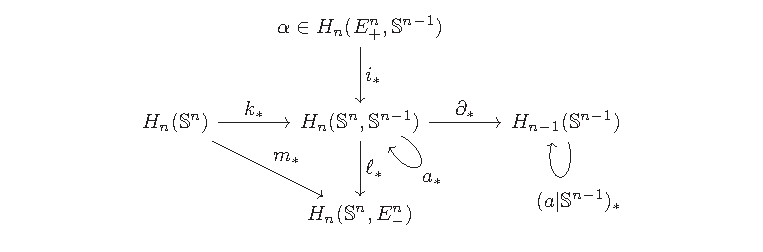
\includegraphics[width=.96\textwidth]{figures/4-14-diagram1.pdf}\end{center}
\sourcepage{292}
令 $\gamma=i_*\alpha+(-1)^{n-1}a_*i_*\alpha\in H_n(S^n,S^{n-1})$。\translatornote{原书把此处 $\gamma$ 所在群误印为 $H_n(E^n_+,S^{n-1})$。}由连接同态自然性及赤道对径映射的度，
\[
\partial_*\gamma=\partial_*i_*\alpha+(-1)^{n-1}(a|_{S^{n-1}})_*\partial_*i_*\alpha=0.
\]
由横向正合性，存在 $\beta\in H_n(S^n)$，使 $k_*\beta=\gamma$。

还需证明 $\beta$ 为生成元。由半球可缩，$m_*:H_n(S^n)\to H_n(S^n,E^n_-)$ 为同构，因此只需证明 $m_*\beta=\ell_*\gamma$ 生成。第一项 $\ell_*i_*\alpha$ 由定理 4.4.11 证明中的同构而生成该群；第二项 $\ell_*a_*i_*\alpha$ 为零，因为映射
\[
(E^n_+,S^{n-1})\xrightarrow{a}(E^n_-,S^{n-1})\longrightarrow(S^n,E^n_-)
\]
经过 $(E^n_-,E^n_-)$ 分解。因此 $\ell_*\gamma$ 确为生成元。

\textbf{步骤 2。}考虑下面的交换图，生成元按步骤 1 选择。
\begin{center}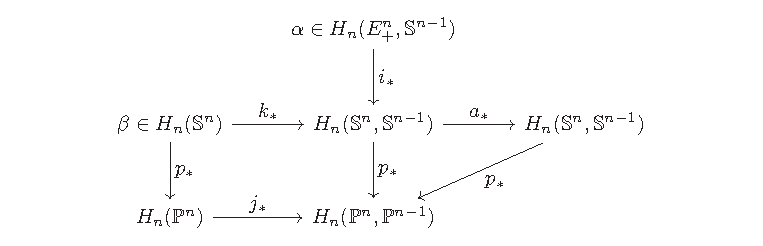
\includegraphics[width=.96\textwidth]{figures/4-14-diagram2.pdf}\end{center}
复合 $pi:(E^n_+,S^{n-1})\to(P^n,P^{n-1})$ 是胞腔特征映射，故 $p_*i_*\alpha$ 为生成元。于是
\[
j_*p_*\beta=p_*k_*\beta
=p_*(i_*\alpha+(-1)^{n-1}a_*i_*\alpha)
=[1+(-1)^{n-1}]p_*i_*\alpha,
\]
其中用了 $pa=p$，结论成立。\hfill$\square$

\sourcepage{293}
\entry{定理}{4.14.9}胞腔边缘 $H_{n+1}(P^{n+1},P^n)\to H_n(P^n,P^{n-1})$ 在 $n$ 偶时为零，在 $n$ 奇时将生成元映为生成元的两倍。

\textbf{证明：}特征映射 $p':(E^{n+1}_+,S^n)\to(P^{n+1},P^n)$ 诱导同构。上半球可缩，连接同态 $H_{n+1}(E^{n+1}_+,S^n)\to\widetilde H_n(S^n)$ 为同构。由连接同态自然性，所求胞腔边缘与上一引理中的 $j_*p_*$ 对应，故得结论。\translatornote{零维处应使用约化同调，才能使这里的连接同态为同构；原书图中统一写成了普通同调。}\hfill$\square$

\entry{定理}{4.14.10}实射影空间的约化同调为
\[
\widetilde H_i(P^{2n+1})\cong\begin{cases}\Z/2,&i\text{ 奇且 }0<i<2n+1,\\\Z,&i=2n+1,\\0,&\text{其他},\end{cases}
\]
\[
\widetilde H_i(P^{2n})\cong\begin{cases}\Z/2,&i\text{ 奇且 }0<i<2n,\\0,&\text{其他},\end{cases}\qquad
\widetilde H_i(P^\infty)\cong\begin{cases}\Z/2,&i>0\text{ 奇},\\0,&\text{其他}.\end{cases}
\]
\textbf{证明：}无限维射影空间的增广胞腔链复形各非负维均为 $\Z$，偶数正维的边缘为乘以 $2$，奇数维边缘为零，增广为恒等同态：
\[
\cdots\xrightarrow{0}\Z\xrightarrow{2}\Z\xrightarrow{0}\Z\xrightarrow{2}\Z\xrightarrow{0}\Z\xrightarrow{1}\Z.
\]
正偶数维没有非零闭链，正奇数维每个链均闭，而边缘恰为生成元的偶数倍。因此约化同调如述。有限维情形只需截断该链复形，即得相应结果。\hfill$\square$

\sourcepage{294}
\entry{引理}{4.14.11}可对 $S^n,P^n$ 三角剖分，使对径映射 $a$ 与商映射 $p$ 都为单纯映射。

\textbf{证明：步骤 1。}先归纳构造复形 $L\subset\R^{n+1}$ 及三角剖分 $k:|L|\to S^n$，使每个坐标反射 $\rho_i$ 都诱导 $L$ 的线性自同构，并与 $k$ 可交换。零维显然。若 $h:|K|\to S^{n-1}$ 已满足要求，取南北极 $w_0,w_1$，令 $L=(w_0*K)\cup(w_1*K)$。定义
\[
k((1-t)x+tw_0)=(\sqrt{1-t^2}\,h(x),t),\quad
k((1-t)x+tw_1)=(\sqrt{1-t^2}\,h(x),-t).
\]
它与所有坐标反射可交换，正是定理 2.9.8 中使用的三角剖分。

\textbf{步骤 2。}对径映射与 $k$ 可交换，并在 $L$ 及其每次重心重分上诱导线性自同构。取重分次数 $N$ 足够大，使每个顶点 $v$ 与 $a(v)$ 的闭星不交。用第 1.4 节的顶点标号方法，给每对 $v,a(v)$ 同一标号，构造商复形 $M$。所得单纯商映射只认同 $x$ 与 $a(x)$，不作其他认同。由于 $k$ 与对径映射可交换，它诱导 $|M|\to P^n$ 的同胚，得到所求三角剖分。\hfill$\square$

下面定义一类三维流形——透镜空间，并计算其同调。它们是少数已完全按同胚类型和同伦类型分类的空间族之一，分类问题稍后讨论。

\sourcepage{295}
\entry{定义}{4.14.12}设 $n,k$ 为互素正整数。把 $B^3$ 中的点写为 $(z,t)$，其中 $z$ 为复数、$t$ 为实数，$|z|^2+t^2\le1$。令 $\lambda=e^{2\pi i/n}$，定义球面上的映射
\[
f(z,t)=(\lambda^kz,-t).
\]
把下半球中每点 $x$ 与上半球中的 $f(x)$ 认同，所得商空间称为\textbf{透镜空间}（lens space），记为 $L(n,k)$。映射 $f$ 先绕竖直轴旋转 $2\pi k/n$，再关于水平面反射。
\begin{center}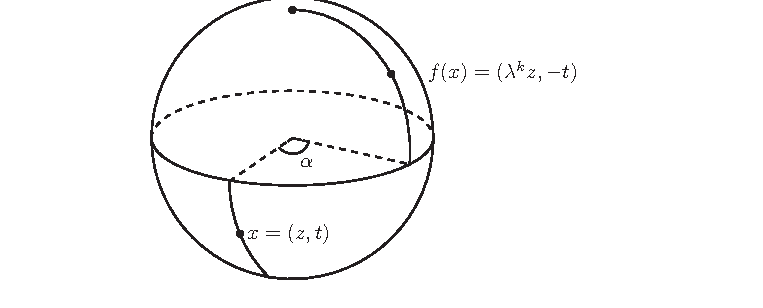
\includegraphics[width=.96\textwidth]{figures/4-14-1.pdf}\\图 4.14.1\end{center}
商映射 $p:B^3\to L(n,k)$ 在球内部不作认同，在两个开半球间成对认同。赤道点 $(z,0)$ 的等价类则为
\[
\{(\lambda^{jk}z,0):j=0,1,\ldots,n-1\}.
\]
因为 $k,n$ 互素，它与 $\{(\lambda^jz,0):0\le j<n\}$ 相同，恰为赤道上均匀分布的 $n$ 点。\translatornote{原书列举这些点时，若干项漏印了因子 $z$；此处用集合公式统一表达。}

\entry{定理}{4.14.13}$L(n,k)$ 是零、一、二、三维各有一个胞腔的 CW 复形。

\sourcepage{296}
\textbf{证明：}先证商映射闭。若 $A\subset B^3$ 闭，其饱和集是下列有限个紧集之并：
\[
A,\quad f(E^2_-\cap A),\quad f^{-1}(E^2_+\cap A),\quad
f^j(A\cap S^1)\ (1\le j<n).
\]
因此饱和集闭，$p(A)$ 闭，商空间正规且 Hausdorff。

取赤道点 $a=(1,0)$，以 $p(a)$ 为零维胞腔。令 $A$ 为从 $a$ 到 $b=(\lambda,0)$ 沿正方向的一段基本弧。限制 $p|_A$ 认同两端，内部则一一对应，所以 $p(\Int A)$ 为一维开胞腔，其特征映射为 $p|_A$。赤道由 $n$ 段这样的基本弧组成，每段内部都同胚地映到同一开胞腔。
\begin{center}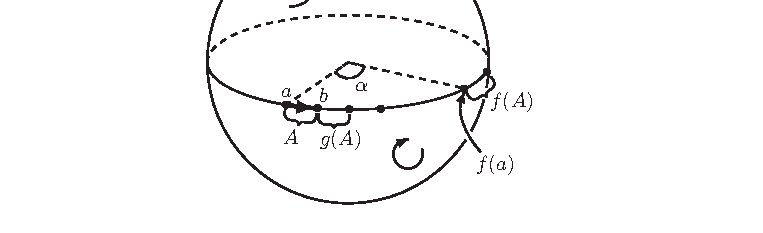
\includegraphics[width=.96\textwidth]{figures/4-14-2.pdf}\\图 4.14.2\end{center}
类似地，$p|_{E^2_-}$ 为二维胞腔的特征映射，内部像为开胞腔；整个 $p$ 为三维胞腔的特征映射，球内部的像为开胞腔。赤道像是一维骨架，球面像是二维骨架。\translatornote{原书称 $A$ 为“两点间的较小弧”。当 $n=1$ 时两端相同，需以完整圆周的一次参数化替代基本弧；可先把球赤道选一点和一条开边，再作同样的胞腔粘合。}\hfill$\square$

\sourcepage{297}
\entry{定理}{4.14.14}若 $X=L(n,k)$，则胞腔链复形为
\[
D_3(X)\xrightarrow{0}D_2(X)\xrightarrow{n}D_1(X)\xrightarrow{0}D_0(X),
\]
每个链群均为无限循环群。因此
\[
H_3(X)\cong\Z,\qquad H_2(X)=0,\qquad H_1(X)\cong\Z/n,\qquad H_0(X)\cong\Z.
\]
所以 $L(n,k)$ 与 $L(m,\ell)$ 若同胚，甚至若仅同伦等价，也必须有 $n=m$。

\textbf{证明：}可对 $B^3,L(n,k)$ 三角剖分，使旋转反射 $f$ 及商映射 $p$ 单纯；证明留作习题。

取基本闭链 $c_1$ 生成 $H_1(A,\Bd A)$，$c_2$ 生成 $H_2(E^2_-,S^1)$，$c_3$ 生成 $H_3(B^3,S^2)$。其像分别生成三个正维胞腔链群。先选 $c_1$ 的符号，使 $\partial c_1=b-a$。令
\[
z_1=c_1+f_\#c_1+\cdots+f_\#^{n-1}c_1.\tag{*}
\]
下面证明它生成 $H_1(S^1)$，然后选择 $c_2$ 的符号使 $\partial c_2=z_1$；再证明
\[
z_2=c_2-f_\#c_2\tag{**}
\]
生成 $H_2(S^2)$，据此选 $c_3$ 使 $\partial c_3=z_2$。

令 $g(z,0)=(\lambda z,0)$。因为赤道上 $f=g^k$，且 $k,n$ 互素，$f$ 的各次迭代将基本弧排列为与 $g$ 各次迭代相同的全部弧。因此
\[
z_1=c_1+g_\#c_1+\cdots+g_\#^{n-1}c_1.
\]
\translatornote{原书称赤道上 $g$ 与 $f$ 相同，这只在 $k\equiv1\pmod n$ 时成立。这里使用的是两者迭代项组成同一集合，因此求和相等。}由 $\partial c_1=g_\#a-a$，得
\[
\partial z_1=\sum_{j=0}^{n-1}(g_\#^{j+1}a-g_\#^ja)=0.
\]
它在基本弧上的限制为 $c_1$，所以是圆周的基本闭链，确为生成元。

再由 (*)，$f_\#z_1=z_1$，故 $\partial z_2=z_1-f_\#z_1=0$。其在下半球上的限制是基本闭链 $c_2$，因此它是球面的基本闭链。这样就能按计划选择 $c_2,c_3$ 的符号。

\sourcepage{298}
现在计算边缘。首先，$\partial p_\#c_1=p_\#b-p_\#a=0$。其次，因为赤道上 $pf^j=p$，
\[
\partial p_\#c_2=p_\#z_1=np_\#c_1.
\]
最后，因为下半球上 $pf=p$，
\[
\partial p_\#c_3=p_\#z_2=p_\#(c_2-f_\#c_2)=0.
\]
这给出所述链复形与同调群。\hfill$\square$

\entry{定理}{4.14.15}若 $k\equiv\pm\ell\pmod n$ 或 $k\ell\equiv\pm1\pmod n$，则透镜空间 $L(n,k)$ 与 $L(n,\ell)$ 同胚。习题 4 将引导证明。

\entry{注}{4.14.16}其逆命题也成立，但证明很困难。Kurt Reidemeister 在 1935 年的论文 [Rei35] 中定义了单纯复形的\textbf{挠率}（torsion），它是组合不变量：有同构重分的复形具有相同挠率。计算透镜空间挠率后，他证明若两个透镜空间的复形有同构重分，则必须满足上述同余条件。

要由此完成同胚分类，还需 E. E. Moise 在二十世纪五十年代关于三维流形仿射结构的研究。其系列论文第五篇 [Moi52] 证明：两个同胚的三角剖分三维流形必有同构的重分。因此透镜空间的同胚分类已知；第 8.9 节将讨论同伦类型分类。

\sourcepage{299--300}
\subsection*{习题}
\begin{enumerate}
\item 证明 $P^n$ 同胚于在 $B^n$ 的边界上认同 $x$ 与 $-x$ 所得商空间。\translatornote{原书把球误印为 $B^3$；按边界 $S^{n-1}$ 及一般维数，应为 $B^n$。}
\item \begin{enumerate}[label=(\alph*)]
\item 证明 $P^n$ 是 $n$ 维流形，$\mathbb CP^n$ 是 $2n$ 维流形。
\item 更一般地，证明有限维齐性 CW 复形是流形。
\end{enumerate}
\item 设 $A$ 为正 $n$ 边形围成的平面闭区域，$B$ 为它的悬挂。将 $L(n,k)$ 描述为 $B$ 的商空间，并推出可三角剖分 $B^3$ 与 $L(n,k)$，使商映射单纯。
\item 按下列步骤证明定理 4.14.15。
\begin{enumerate}[label=(\alph*)]
\item 考虑 $B^3$ 中反射 $(z,t)\mapsto(z,-t)$，证明 $k\equiv\pm\ell\pmod n$ 的情形。
\item 为方便设 $1\le k<n$。取以 $\Z/n$ 为指标的 $n$ 个不交三维单形 $a_ib_ic_id_i$，见图 4.14.3。证明 $L(n,k)$ 可按下列两步得到：先逐一将面 $a_ib_id_i$ 与 $a_{i+1}b_{i+1}c_{i+1}$ 按顶点顺序线性粘合，再把 $c_id_ib_i$ 与 $c_{i+k}d_{i+k}a_{i+k}$ 按顺序线性粘合。
\item 将这些单形改按 $a_kb_kc_kd_k,a_{2k}b_{2k}c_{2k}d_{2k},\ldots,a_{nk}b_{nk}c_{nk}d_{nk}$ 排列，见图 4.14.4。先作 (b) 的第二次粘合，再作第一次，证明所得描述为 $L(n,\ell)$，其中 $1\le\ell<n$ 且 $k\ell\equiv1\pmod n$。
\item 完成定理的证明。
\end{enumerate}
\item 证明 $L(n,k)$ 是紧三维流形。
\begin{center}
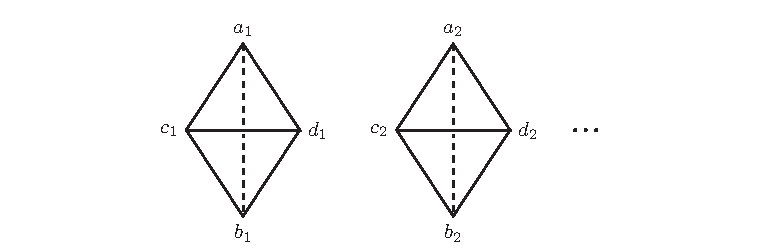
\includegraphics[width=.96\textwidth]{figures/4-14-3.pdf}\\图 4.14.3\par\medskip
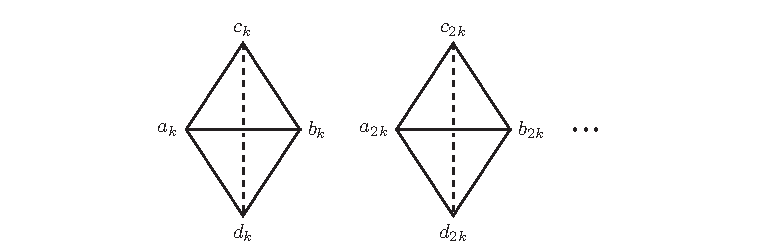
\includegraphics[width=.96\textwidth]{figures/4-14-4.pdf}\\图 4.14.4
\end{center}
\item 实 $n$ 维射影空间与复 $n$ 维射影空间有什么关系？
\item $n$ 维欧氏空间中的任一对象，在实 $n$ 维射影空间中都有一个像。解释这一点。单位球、单位立方体的像分别是什么？
\end{enumerate}

\chapter{上同调}
\section{引言}
\sourcepage{301}
我们已经给每个拓扑空间 $X$ 指定了一列阿贝尔群，称为同调群。现在再给它指定另一列阿贝尔群，称为\textbf{上同调群}（cohomology groups）。上同调的定义比同调晚得多，原因不难理解：它在几何上远不如同调自然，其起源在代数而非几何。在稍后将精确说明的某种代数意义下，它与同调互为“对偶”。过去拓扑学家曾把这些群元素的代表称为“伪闭链”等，似乎对它们能否成为正当研究对象抱有疑虑。后来逐渐明白，上同调既有理论意义，也有实际用途；它比同调更细致，也更深刻、更有力。本章将研究它。

流形的对偶定理、拓扑与微分几何之间的联系（de Rham 定理）、拓扑与分析之间的联系（层系数上同调），都用上同调表述。甚至空间的同胚分类、映射的同伦分类等纯拓扑问题，上同调也能提供丰富信息。以后将回到其中一些问题。

本章假定读者熟悉第 3.7 节的范畴与函子语言。

\section{Hom 函子}
\sourcepage{301--302}
任意两个阿贝尔群 $A,G$ 都确定第三个阿贝尔群 $\operatorname{Hom}(A,G)$，即从 $A$ 到 $G$ 的所有同态组成的群。它将在上同调定义中起核心作用。本节研究其性质。

\entry{定义}{5.2.1}对同态 $\varphi,\psi:A\to G$，按值相加定义 $(\varphi+\psi)(a)=\varphi(a)+\psi(a)$。这仍为同态，因为它将零映到零，且
\[
(\varphi+\psi)(a+b)=\varphi(a)+\psi(a)+\varphi(b)+\psi(b).
\]
所有同态在此加法下构成阿贝尔群 $\operatorname{Hom}(A,G)$。零元是零同态，$\varphi$ 的负元将 $a$ 映为 $-\varphi(a)$。可称其为同态群，通常简称 Hom。

\entry{例}{5.2.2}映射 $I:\operatorname{Hom}(\Z,G)\to G$，$I(\varphi)=\varphi(1)$，为同构。若 $A$ 是以 $e_1,\ldots,e_n$ 为基的有限秩自由阿贝尔群，则 $\varphi\mapsto(\varphi(e_1),\ldots,\varphi(e_n))$ 给出 $\operatorname{Hom}(A,G)\cong G^n$。这一同构依赖基的选择，因此并非相对于 $A$ 的自然同构。若自由基为无限族 $\{e_\alpha\}_{\alpha\in J}$，相同映射得到的是直积 $\prod_{\alpha\in J}G$，而非直和（定义见第 1.5 节）。后面将把这些事实表述为定理。

\entry{定义}{5.2.3}同态 $f:A\to B$ 诱导反方向的\textbf{对偶同态}
\[
\overline f:\operatorname{Hom}(B,G)\to\operatorname{Hom}(A,G),\qquad
\overline f(\varphi)=\varphi\circ f.
\]
复合仍为同态，故映射有意义。而且
\[
[\overline f(\varphi+\psi)](a)=\varphi(f(a))+\psi(f(a))
=[\overline f(\varphi)](a)+[\overline f(\psi)](a),
\]
所以 $\overline f$ 本身为群同态。\translatornote{原书在这里把“$\overline f$ 为同态”写成“$f\mapsto\overline f$ 为同态”，而所给计算验证的是前者。}

\sourcepage{303}
固定 $G$ 后，$A\mapsto\operatorname{Hom}(A,G)$、$f\mapsto\overline f$ 构成阿贝尔群范畴到自身的反变函子。恒等映射的对偶仍为恒等映射；若 $h=g\circ f$，则
\[
\overline h(\varphi)=\varphi\circ g\circ f=\overline f\,\overline g(\varphi),
\]
所以复合顺序反转。以下列出几个推论。

\entry{定理}{5.2.4}设 $g:B\to C$ 为阿贝尔群同态。
\begin{enumerate}[label=(\alph*)]
\item 若 $g=0$，则 $\overline g=0$。
\item 若 $g$ 为同构，则 $\overline g$ 为同构。
\item 若 $g$ 满射，则 $\overline g$ 单射。因此 $B\xrightarrow{g}C\to0$ 正合蕴含 $\operatorname{Hom}(B,G)\xleftarrow{\overline g}\operatorname{Hom}(C,G)\leftarrow0$ 正合。
\end{enumerate}
\textbf{证明：}前两点直接成立。若 $\overline g(\psi)=\psi g=0$，则对每个 $b$，$\psi(g(b))=0$；由 $g$ 满射可知 $\psi=0$，证明 (c)。\hfill$\square$

\entry{定理}{5.2.5}若 $A\xrightarrow{f}B\xrightarrow{g}C\to0$ 正合，则
\[
\operatorname{Hom}(A,G)\xleftarrow{\overline f}\operatorname{Hom}(B,G)
\xleftarrow{\overline g}\operatorname{Hom}(C,G)\leftarrow0
\]
正合。若另外 $f$ 单射，且原短正合列分裂，则 $\overline f$ 满射，对偶短正合列也分裂。

\sourcepage{304}
\textbf{证明：}$\overline g$ 单射已证。由 $gf=0$，有 $\overline f\,\overline g=0$。反过来，若 $\overline f(\psi)=\psi f=0$，则 $\psi$ 在 $f(A)$ 上为零，故诱导 $\psi':B/f(A)\to G$。正合性使 $g$ 诱导同构 $g':B/f(A)\to C$。令 $\varphi=\psi'(g')^{-1}$，则 $\overline g(\varphi)=\psi$，得到正合性。

若原列分裂，取 $\pi:B\to A$，使 $\pi f=\operatorname{id}_A$。于是 $\overline f\,\overline\pi=\operatorname{id}_{\operatorname{Hom}(A,G)}$，所以 $\overline f$ 满射，而 $\overline\pi$ 给出对偶列的分裂。\hfill$\square$

一般的短正合列对偶后未必仍短正合。例如 $0\to\Z\xrightarrow{2}\Z\to\Z/2\to0$ 正合，但取 $G=\Z$，对偶映射把每个同态变为取值均为偶数的同态，故不满射。

Hom 也可视为两个变量的函子，具有混合变性：对第一个变量反变，对第二个变量协变。

\entry{定义}{5.2.6}给定 $\alpha:A\to A'$、$\beta:G'\to G$，定义
\[
\operatorname{Hom}(\alpha,\beta):\operatorname{Hom}(A',G')\to\operatorname{Hom}(A,G),\qquad
\varphi'\mapsto\beta\circ\varphi'\circ\alpha.
\]
它确为群同态。恒等映射诱导恒等同态；若还有 $\alpha':A'\to A''$、$\beta':G''\to G'$，则
\[
\operatorname{Hom}(\alpha'\alpha,\beta\beta')=
\operatorname{Hom}(\alpha,\beta)\circ\operatorname{Hom}(\alpha',\beta'),
\]
因为两边均将 $\varphi''$ 映到 $\beta\beta'\varphi''\alpha'\alpha$。原先的对偶同态就是 $\overline\alpha=\operatorname{Hom}(\alpha,i_G)$。只对第二变量考虑的协变函子留作习题。

\sourcepage{305}
\entry{定理}{5.2.7}
\begin{enumerate}[label=(\alph*)]
\item 存在同构
\[
\operatorname{Hom}(\bigoplus_{\alpha\in J}A_\alpha,G)\cong\prod_{\alpha\in J}\operatorname{Hom}(A_\alpha,G),\qquad
\operatorname{Hom}(A,\prod_{\alpha\in J}G_\alpha)\cong\prod_{\alpha\in J}\operatorname{Hom}(A,G_\alpha).
\]
\item $\lambda:\operatorname{Hom}(\Z,G)\to G$，$\lambda(\varphi)=\varphi(1)$，是自然同构。
\item 若 $f_m:\Z\to\Z$ 为乘以正整数 $m$，则 $\overline f_m$ 在 $\operatorname{Hom}(\Z,G)$ 上也是乘以 $m$。
\item 若 $g_m:G\to G$ 为乘以 $m$，则 $\operatorname{Hom}(\Z/m,G)\cong\ker g_m$。
\end{enumerate}
\textbf{证明：}(a) 来自关于直和、直积同态的标准代数事实：第一式取各直和因子上的限制，第二式取各坐标分量。

(b) 一个从 $\Z$ 出发的同态由 $1$ 的像唯一决定，该像可任取，且取值映射为同态，所以为同构。

(c) 直接计算 $[\overline f_m(\varphi)](x)=\varphi(mx)=m\varphi(x)$。

(d) 对正合列 $\Z\xrightarrow{f_m}\Z\to\Z/m\to0$ 应用定理 5.2.5，得 $\operatorname{Hom}(\Z/m,G)\cong\ker\overline f_m$。由 (b)、(c) 将它识别为 $\ker g_m$。\hfill$\square$

\sourcepage{306}
(a) 中的同构也自然。例如给定 $\varphi_\alpha:A_\alpha\to B_\alpha$、$\psi:H\to G$，第一个同构将 $\operatorname{Hom}(\bigoplus\varphi_\alpha,\psi)$ 与 $\prod\operatorname{Hom}(\varphi_\alpha,\psi)$ 对应，构成交换图；第二个同构同理。\translatornote{原书本段将定理编号误引为 5.2.4(a)，应为 5.2.7(a)。}

因此，若 $A$ 有限生成，将它分解为循环群的有限直和，就能用 $\operatorname{Hom}(\Z,G)\cong G$ 和 $\operatorname{Hom}(\Z/m,G)\cong\ker g_m$ 计算 Hom。若 $G$ 也有限生成，可进一步写成循环群直和。需要下面的引理，证明留给读者。

\entry{引理}{5.2.8}设 $m,n>0$，$d=\gcd(m,n)$，$h_m:\Z/n\to\Z/n$ 为乘以 $m$，则有正合列
\[
0\longrightarrow\Z/d\longrightarrow\Z/n\xrightarrow{h_m}\Z/n\longrightarrow\Z/d\longrightarrow0.
\]

\entry{定义}{5.2.9}若对每个 $x\in G$ 和每个正整数 $n$，都存在 $y\in G$ 使 $ny=x$，则称阿贝尔群 $G$ \textbf{可除}（divisible）。例如有理数加法群、实数加法群都可除。

\entry{定义}{5.2.10}记 $S^1=\R/\Z$，称为\textbf{圆周群}（circle group）。它作为加法群同构于模为 $1$ 的复数乘法群，也是可除群。可除群将在后面多次出现。

\sourcepage{307}
\entry{定理}{5.2.11}若 $G$ 可除，则任意短正合列 $0\to A\to B\to C\to0$ 的对偶序列
\[
0\leftarrow\operatorname{Hom}(A,G)\leftarrow\operatorname{Hom}(B,G)\leftarrow\operatorname{Hom}(C,G)\leftarrow0
\]
也正合。证明留作习题 4。

\subsection*{习题}
\begin{enumerate}
\item 若 $T$ 为 $G$ 的挠子群，证明 $\operatorname{Hom}(G,\Z)\cong\operatorname{Hom}(G/T,\Z)$。
\item 固定 $G$，考虑协变函子 $A\mapsto\operatorname{Hom}(G,A)$、$f\mapsto\operatorname{Hom}(i_G,f)$。
\begin{enumerate}[label=(\alph*)]
\item 证明它保持 $0\to A\to B\to C$ 的正合性。
\item 证明它保持分裂短正合列。
\end{enumerate}
\item \begin{enumerate}[label=(\alph*)]
\item 设 $d=\gcd(m,n)$，证明乘法同态 $h_m:\Z/n\to\Z/n$ 的核由 $\{n/d\}$ 生成。
\item 证明循环群的商群仍循环。
\item 证明引理 5.2.8。
\end{enumerate}
\item 按下列步骤证明定理 5.2.11。
\begin{enumerate}[label=(\alph*)]
\item 证明只需说明：若 $A\subset B$，则每个 $\varphi:A\to G$ 都可延拓为同态 $\psi:B\to G$。
\item 当 $B$ 由 $A$ 及一个额外元素 $b$ 生成时证明这一点。
\item 设 $\mathcal B$ 是 $B$ 的一族按包含关系全序的子群，对每个 $H\in\mathcal B$ 有同态 $\psi_H:H\to G$，任意两个在公共定义域上一致。证明这些子群的并仍为子群，且诸同态合成其上的同态。
\item 用 Zorn 引理完成证明。〔不熟悉者可参考 [Mun00] 第 70 页。〕
\end{enumerate}
\item 设 $R$ 为有单位元的交换环，$A,B$ 为 $R$ 模（定义见第 5.9 节）。
\begin{enumerate}[label=(\alph*)]
\item 以 $\operatorname{Hom}_R(A,B)$ 表示 $R$ 模同态全体，证明它自然成为 $R$ 模；若 $f,g$ 为模同态，证明 $\operatorname{Hom}(f,g)$ 也为模同态。
\item 陈述并证明定理 5.2.5、5.2.7 的 $R$ 模版本。
\item 特别设 $R$ 为域 $F$。此时上述模都是向量空间。证明每个短正合列均分裂，故 $\operatorname{Hom}_F$ 保持正合列。
\end{enumerate}
\item 证明可除群的直积可除，可除群的商群也可除。
\end{enumerate}

\section{单纯上同调群}
\sourcepage{308}
本节定义单纯复形的上同调群，并计算一些初等例子。

\entry{定义}{5.3.1}设 $K$ 为单纯复形，$G$ 为阿贝尔群。以 $G$ 为系数的 $p$ 维\textbf{上链群}（cochain group）为
\[
C^p(K;G)=\operatorname{Hom}(C_p(K),G).
\]
\textbf{上边缘算子}（coboundary operator）$\delta:C^p(K;G)\to C^{p+1}(K;G)$ 是边缘算子 $\partial:C_{p+1}(K)\to C_p(K)$ 的对偶，因此使维数升高一维。记其核为\textbf{上闭链群} $Z^p(K;G)$，像为\textbf{上边缘群} $B^{p+1}(K;G)$。由 $\partial^2=0$ 得 $\delta^2=0$，于是定义\textbf{上同调群}
\[
H^p(K;G)=Z^p(K;G)/B^p(K;G).
\]
若系数为整数，通常省略 $G$。

\sourcepage{309}
对于上链 $c^p$ 与链 $c_p$，通常用对偶配对 $\langle c^p,c_p\rangle$ 表示上链在链上的取值。此时上边缘的定义为
\[
\langle\delta c^p,d_{p+1}\rangle=\langle c^p,\partial d_{p+1}\rangle.
\]
这个定义确实很代数化，但仍可在一定程度上作几何理解。

任意为 $K$ 的 $p$ 维单形定向，得到 $C_p(K)$ 的自由基 $\{\sigma_\alpha\}$。链必须是有限和 $\sum n_\alpha\sigma_\alpha$；上链则由它在每个基元上的值 $g_\alpha\in G$ 唯一决定，这些值可以任意指定，不要求仅有限个非零。

令整数\textbf{初等上链} $\sigma_\alpha^*$ 在 $\sigma_\alpha$ 上取 $1$，在其余基元上取 $0$。对 $g\in G$，用 $g\sigma_\alpha^*$ 表示在该基元上取 $g$、其他处为零的上链。于是可将任意上链写成可能无限的\emph{形式和}
\[
c^p=\sum_\alpha g_\alpha\sigma_\alpha^*.
\]
其依据是：若 $C_\alpha$ 为 $\sigma_\alpha$ 生成的无限循环群，则
\[
C^p(K;G)=\operatorname{Hom}(\bigoplus C_\alpha,G)
\cong\prod_\alpha\operatorname{Hom}(C_\alpha,G).
\]
形式和只是用来替代直积的元组记号。

这种记号在计算上边缘时很方便，且确有
\[
\delta c^p=\sum_\alpha g_\alpha\delta\sigma_\alpha^*.
\]
为验证，对任意有向 $(p+1)$ 维单形 $\tau$，写 $\partial\tau=\sum_{i=0}^{p+1}\epsilon_i\sigma_{\alpha_i}$，$\epsilon_i=\pm1$。于是
\[
\langle\delta c^p,\tau\rangle=\sum_{i=0}^{p+1}\epsilon_i g_{\alpha_i}.
\]
右侧形式和中只有对应这有限个面的项在 $\tau$ 上非零，取值同为此和。因此公式有意义并成立。

\sourcepage{310}
故只需计算初等上链的上边缘：
\[
\delta\sigma^*=\sum_j\epsilon_j\tau_j^*,
\]
其中 $\tau_j$ 遍历所有以 $\sigma$ 为面的 $(p+1)$ 维单形，$\epsilon_j$ 是 $\sigma$ 在 $\partial\tau_j$ 中的符号。对任意单形取值即可验证。下面只作少量计算，一般计算问题留待后面。

\entry{例}{5.3.2}取图 5.3.1 的复形，顶点为 $v_i$，边 $e_i$ 与二维单形 $\sigma_i$ 均按图定向。边 $e_5$ 在 $\partial\sigma_1$、$\partial\sigma_2$ 中的系数分别为 $1,-1$，故
\[
\delta e_5^*=\sigma_1^*-\sigma_2^*.
\]
\begin{center}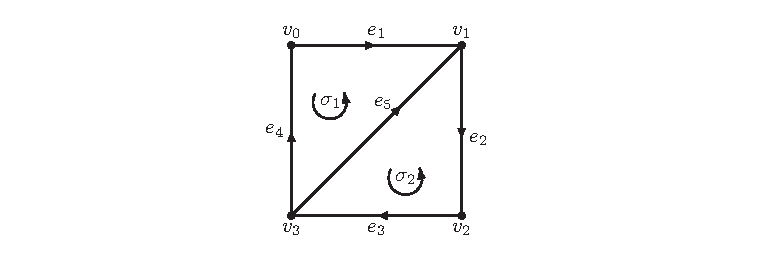
\includegraphics[width=.96\textwidth]{figures/5-3-1.pdf}\\图 5.3.1\end{center}
类似地，$\delta v_1^*=e_1^*+e_5^*-e_2^*$。由于无三维单形，$\sigma_1^*,\sigma_2^*$ 均为上闭链；它们也都是上边缘，因为 $\delta e_1^*=-\sigma_1^*$、$\delta e_3^*=-\sigma_2^*$。

\sourcepage{311}
一维上链 $c^1=e_1^*+e_5^*-e_3^*$ 也是上闭链，而且等于 $\delta(v_1^*+v_2^*)$。零维上链 $c^0=v_0^*+v_1^*+v_2^*+v_3^*$ 也是上闭链，但不是上边缘，因为不存在负一维上链。

\entry{定义}{5.3.3}若两个上链之差为上边缘，称它们\textbf{上同调}（cohomologous）。例如上式说明 $\sigma_1^*$ 与 $\sigma_2^*$ 上同调。

\entry{例}{5.3.4}考虑图 5.3.2 中稍简化的环面三角剖分。令
\[
z^1=e_1^*+e_2^*+e_3^*+e_4^*+e_5^*+e_6^*,\qquad
d^1=e_7^*+e_8^*+e_9^*+e_{10}^*+e_{11}^*+e_{12}^*.
\]
它们都是上闭链，而且 $\delta(c^*+h^*+j^*)=z^1-d^1$，所以彼此上同调。
\begin{center}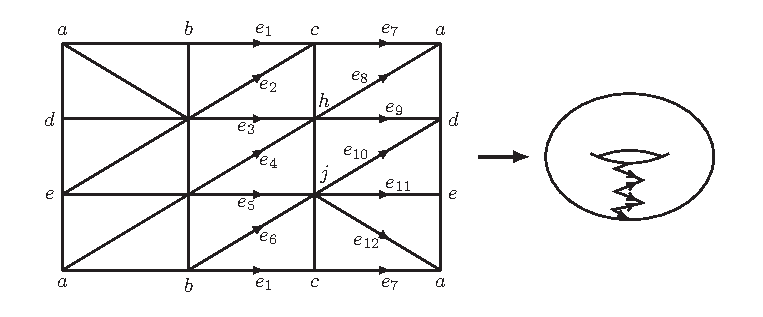
\includegraphics[width=.96\textwidth]{figures/5-3-2.pdf}\\图 5.3.2\end{center}
这说明：一维闭链可以想成闭曲线，而一维上闭链更适合想成一道栅栏！第 5.8 节将证明 $z^1$ 代表 $H^1(T)$ 的一个生成元。

\sourcepage{312}
\entry{例}{5.3.5}计算图 5.3.3 的复形 $K$。一般零维上链为 $c^0=\sum n_iv_i^*$，其上边缘在 $e_1$ 上取 $n_2-n_1$，在 $e_2$ 上取 $n_3-n_2$，依此类推。所以它上闭当且仅当所有 $n_i$ 相等。没有零维上边缘，故 $H^0(K)\cong\Z$，生成元由 $\sum v_i^*$ 代表。
\begin{center}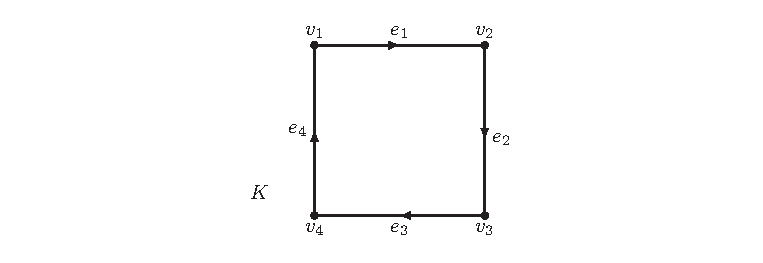
\includegraphics[width=.96\textwidth]{figures/5-3-3.pdf}\\图 5.3.3\end{center}
每个一维上链都上闭。各 $e_i^*$ 都与 $e_1^*$ 上同调，例如 $\delta(v_4^*+v_1^*)=e_3^*-e_1^*$。因此每个一维上链都上同调于 $e_1^*$ 的某个倍数。

这个倍数仅在为零时可能为上边缘：取闭链 $z=e_1+e_2+e_3+e_4$。任意零维上链满足 $\langle\delta c^0,z\rangle=\langle c^0,\partial z\rangle=0$，而 $\langle ne_1^*,z\rangle=n$。所以 $H^1(K)\cong\Z$，由 $e_1^*$ 的类生成，也可由其他任一边的初等上链生成。这一论证同样适用于任意多边形。

\entry{例}{5.3.6}上一例中同调与上同调群相同，下面说明一般并非如此。取图 5.3.4 的 Klein 瓶 $S$。已知 $H_2(S)=0$，但 $H^2(S)$ 非零。

\sourcepage{313}
\begin{center}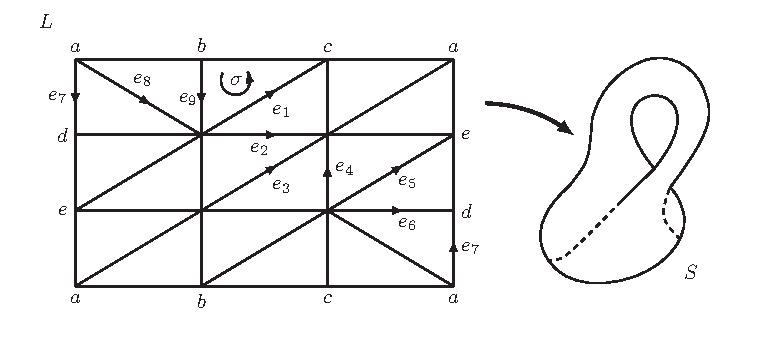
\includegraphics[width=.96\textwidth]{figures/5-3-4.pdf}\\图 5.3.4\end{center}
将矩形 $L$ 的二维单形逆时针定向，并把定向传到 $S$，记其和为 $\gamma$。它不是闭链，因为 $\partial\gamma=2z_1$，其中 $z_1=[a,d]+[d,e]+[e,a]$。

取图中的一个有向二维单形 $\sigma$。因无三维单形，$\sigma^*$ 上闭。对任意一维上链，
\[
\langle\delta c^1,\gamma\rangle=\langle c^1,\partial\gamma\rangle=2\langle c^1,z_1\rangle
\]
为偶数，而 $\langle\sigma^*,\gamma\rangle=1$，故 $\sigma^*$ 不是上边缘。它实际上代表一个二阶元素：可核对图中 $e_1^*+\cdots+e_9^*$ 的上边缘恰为 $2\sigma^*$。

\entry{定理}{5.3.7}$H^0(K;G)$ 等于所有在同一连通分支的顶点上取相同值的零维上链组成的群。特别地，若 $|K|$ 连通，则 $H^0(K)\cong\Z$，生成元是在每个顶点上取值 $1$ 的上链。

\textbf{证明：}没有零维上边缘，所以只需确定零维上闭链。若顶点 $v,w$ 属于同一分支，可取一维链 $c_1$ 使 $\partial c_1=v-w$。对上闭链 $c^0$，
\[
0=\langle\delta c^0,c_1\rangle=\langle c^0,v\rangle-\langle c^0,w\rangle.
\]
反之，若它在同一分支各顶点上相等，则对每条有向边 $\sigma$，$\langle\delta c^0,\sigma\rangle=\langle c^0,\partial\sigma\rangle=0$，所以 $\delta c^0=0$。\hfill$\square$

\sourcepage{314}
因此，$H^0(K)$ 是每个连通分支对应一个 $\Z$ 的直积，而 $H_0(K)$ 是这些群的直和。这又是同调与上同调不同的一个例子。

\entry{定义}{5.3.8}将标准增广 $C_1(K)\xrightarrow{\partial_1}C_0(K)\xrightarrow{\epsilon}\Z$ 对偶化，得
\[
C^1(K;G)\xleftarrow{\delta^1}C^0(K;G)\xleftarrow{\overline\epsilon}G.
\]
称 $\overline\epsilon$ 为\textbf{余增广}（coaugmentation）。它单射，且 $\delta^1\overline\epsilon=0$。定义\textbf{约化上同调}：正维与普通上同调相同，而
\[
\widetilde H^0(K;G)=\ker\delta^1/\operatorname{im}\overline\epsilon.
\]

\entry{定理}{5.3.9}若 $|K|$ 连通，则 $\widetilde H^0(K;G)=0$。更一般地，$H^0(K;G)\cong\widetilde H^0(K;G)\oplus G$。

\textbf{证明：}连通时，增广链列 $C_1(K)\to C_0(K)\to\Z\to0$ 正合，对偶列也正合，所以约化零维上同调为零。其余结论留作习题。\hfill$\square$

\subsection*{习题}
\begin{enumerate}
\item 对例 5.3.2 的复形，求每一维上闭链群的一组基，并证明正维上同调为零。
\item 核对例 5.3.2、定义 5.3.3 附近及例 5.3.4 的计算。\translatornote{原书把 5.3.3 也称为例，实际上它是定义。}
\item \begin{enumerate}[label=(\alph*)]
\item 设 $C_1\xrightarrow{\varphi}C_0\xrightarrow{\epsilon}\Z$ 满足 $\epsilon\varphi=0$，且 $\epsilon$ 满射。考察对偶列，证明 $\operatorname{im}\overline\epsilon$ 是 $\operatorname{Hom}(C_0,G)$ 的直和项，因而也是 $\ker\overline\varphi$ 的直和项。〔见第 1.8 节习题。〕
\item 推出 $\ker\overline\varphi\cong(\ker\overline\varphi/\operatorname{im}\overline\epsilon)\oplus G$，特别地 $H^0(K;G)\cong\widetilde H^0(K;G)\oplus G$。
\end{enumerate}
\item 设 $K$ 的多面体为实数轴，顶点为整数，$\sigma_n=[n,n+1]$。对任意上链 $\sum_{i=-\infty}^{\infty}a_i\sigma_i^*$，显式找一个零维上链以它为上边缘，从而证明 $H^1(K)=0$。
\item 〔*〕设 $K$ 为有限复形。
\begin{enumerate}[label=(\alph*)]
\item 用第 1.12 节链复形标准基定理，以 Betti 数和挠系数表示 $H^p(K)$。
\item 以相同数据表示 $H^p(K;G)$，答案涉及 $G$、$G/mG$ 及乘以 $m$ 的核。
\item 对环面、Klein 瓶、射影空间计算 $H^p(X;G)$。
\end{enumerate}
\item 计算二维球面的上同调。高维球面更难直接计算，为什么？
\end{enumerate}

\section{相对上同调}
\sourcepage{315--316}
继续讨论单纯上同调，定义相对群、单纯映射诱导的同态及长正合列。它们有些方面类似相对同调，有些方面却相当不同。

\entry{定义}{5.4.1}若 $K_0$ 为 $K$ 的子复形，则\textbf{相对上链群}为
\[
C^p(K,K_0;G)=\operatorname{Hom}(C_p(K,K_0),G).
\]
相对上边缘为相对边缘的对偶，记为 $\delta$。其核、像分别为相对上闭链群 $Z^p$、相对上边缘群 $B^{p+1}$，定义
\[
H^p(K,K_0;G)=Z^p(K,K_0;G)/B^p(K,K_0;G).
\]
相对上链的几何理解与相对链不同。链群短正合列
\[
0\to C_p(K_0)\xrightarrow{i}C_p(K)\xrightarrow{j}C_p(K,K_0)\to0
\]
因商群自由而分裂。对偶后仍为分裂短正合列
\[
0\leftarrow C^p(K_0;G)\xleftarrow{\overline i}C^p(K;G)
\xleftarrow{\overline j}C^p(K,K_0;G)\leftarrow0.
\]
于是，相对上链群自然是绝对上链群的\emph{子群}，而子复形的上链群自然是其\emph{商群}。

具体地，从商链群到 $G$ 的同态，恰对应于在 $C_p(K_0)$ 上为零的同态。因此可以把相对上链认同为在 $K_0$ 的每个有向单形上都为零的上链。某种意义上，它们由 $K\setminus K_0$ “承载”。这一子群被 $\delta$ 保持：若 $\tau$ 是 $K_0$ 的单形，则其边缘也在 $K_0$ 内，所以 $\langle\delta c^p,\tau\rangle=\langle c^p,\partial\tau\rangle=0$。

\sourcepage{317}
因此投影 $j$ 的对偶是包含映射，而包含 $i$ 的对偶是把上链限制到 $C_p(K_0)$ 的限制映射。

若 $f:(K,K_0)\to(L,L_0)$ 为单纯映射，其相对链映射 $f_\#$ 的对偶记为 $f^\#$。由 $f_\#\partial=\partial f_\#$，得 $\delta f^\#=f^\#\delta$。它称为\textbf{上链映射}（cochain map），将上闭链、上边缘分别映为上闭链、上边缘，诱导
\[
f^*:H^p(L,L_0;G)\to H^p(K,K_0;G).
\]
函子性质在上链层次已经成立：恒等映射诱导恒等，而 $(g\circ f)^\#=f^\#g^\#$。

\entry{定理}{5.4.2}存在长正合列
\[
\cdots\leftarrow H^p(K_0;G)\leftarrow H^p(K;G)\leftarrow H^p(K,K_0;G)
\xleftarrow{\delta^*}H^{p-1}(K_0;G)\leftarrow\cdots.
\]
若 $K_0\ne\varnothing$，约化上同调也有类似序列。单纯映射诱导相应长正合列之间的同态。

\sourcepage{318}
\textbf{证明：}将逐维分裂的上链短正合列与各 $\delta$ 排成交换图，应用之字形引理（引理 3.3.2）。虽然箭头方向与链复形相反，方法完全相同，连接同态 $\delta^*$ 使维数增加一维。

对约化情形，在零维下面补上短正合列 $0\leftarrow G\xleftarrow{\operatorname{id}}G\leftarrow0\leftarrow0$，并以余增广连接到零维上链列，即可作同样论证。余增广单射，所以负一维没有非零上同调。自然性也由之字形引理得到。\hfill$\square$

\entry{例}{5.4.3}取图 5.4.1 的正方形复形 $K$ 及其边界 $K_0$。相对上链就是在边界上为零的上链。二维相对上闭链由 $\sigma_1^*,\sigma_2^*$ 生成，一维相对上链由 $e_5^*$ 生成，且 $\delta e_5^*=\sigma_1^*-\sigma_2^*$。所以 $H^2(K,K_0)\cong\Z$，生成元为两者共同的上同调类。
\begin{center}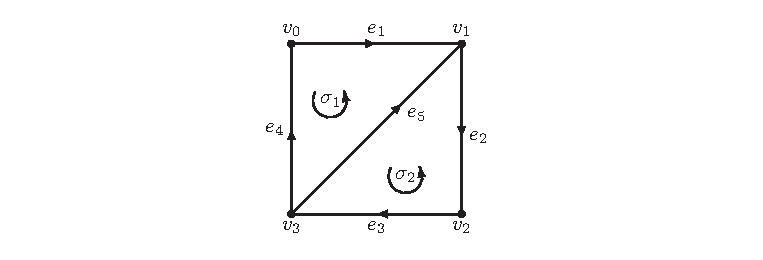
\includegraphics[width=.96\textwidth]{figures/5-4-1.pdf}\\图 5.4.1\end{center}
没有非零相对一维上闭链，也没有非零相对零维上链，故 $H^1(K,K_0)=H^0(K,K_0)=0$。

\sourcepage{319}
结合边界圆周的计算，长正合列的一段变为
\[
0\leftarrow H^2(K)\leftarrow\Z\xleftarrow{\delta^*}\Z\leftarrow H^1(K)\leftarrow0.
\]
还需计算连接同态。$H^1(K_0)$ 由 $e_1^*$ 的类生成。先将它延拓为 $K$ 上同名上链，再取上边缘，并视为相对上链，即得到 $\delta^*$。由 $\delta e_1^*=-\sigma_1^*$，可知连接同态为同构。因此两个未知群 $H^2(K),H^1(K)$ 都为零。

\entry{例}{5.4.4}考虑图 5.4.2 的 Möbius 带 $M$ 及其边界 $E$。计算空间偶与空间本身的上同调。
\begin{center}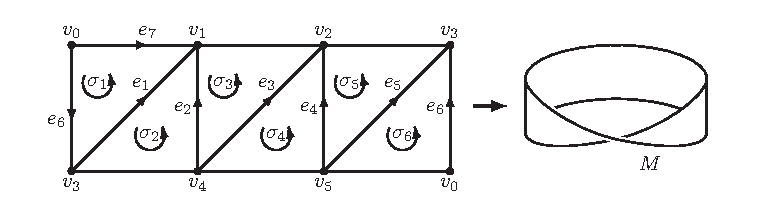
\includegraphics[width=.96\textwidth]{figures/5-4-2.pdf}\\图 5.4.2\end{center}
二维相对上闭链以六个 $\sigma_i^*$ 为基，一维相对上链以 $e_1^*,\ldots,e_6^*$ 为基。改用基
\[
\sigma_1^*,\ \sigma_1^*-\sigma_2^*,\ \ldots,\ \sigma_5^*-\sigma_6^*
\]
及
\[
e_1^*,\ldots,e_5^*,\ e_1^*+\cdots+e_6^*.
\]
有 $\delta e_i^*=\sigma_i^*-\sigma_{i+1}^*$（$1\le i\le5$），且最后一个基元的上边缘为 $2\sigma_1^*$。因此 $H^2(M,E)\cong\Z/2$，由 $\sigma_1^*$ 的类生成。上边缘把一维基映为一个子群的基，故一维核为零，$H^1(M,E)=0$；零维相对上链为零，故 $H^0(M,E)=0$。

\sourcepage{320}
边界 $E$ 是六边形，故 $H^1(E)\cong\Z$、$H^2(E)=0$。长正合列为
\[
0\leftarrow H^2(M)\leftarrow\Z/2\xleftarrow{\delta^*}\Z\leftarrow H^1(M)\leftarrow0.
\]
取边界边 $e_7$，其初等上链的类生成 $H^1(E)$。延拓后直接计算 $\delta e_7^*=-\sigma_1^*$，所以连接同态满射。由正合性，$H^2(M)=0$，$H^1(M)\cong\Z$。

下面定义以后会多次出现的伪流形。

\entry{定义}{5.4.5}若单纯偶 $(K,K_0)$ 满足下列条件，称为\textbf{相对 $n$ 维伪流形}（relative pseudo $n$-manifold）：
\begin{enumerate}[label=(\arabic*)]
\item $\overline{|K|\setminus|K_0|}$ 为一些 $n$ 维单形之并。
\item 每个不在 $K_0$ 中的 $(n-1)$ 维单形，恰为两个 $n$ 维单形的面。
\item 任意两个不在 $K_0$ 中的 $n$ 维单形 $\sigma,\sigma'$，都可由序列 $\sigma=\sigma_0,\ldots,\sigma_k=\sigma'$ 连接，其中各单形不在 $K_0$ 中，且每个相邻交都是不在 $K_0$ 中的 $(n-1)$ 维单形。
\end{enumerate}
若 $K_0=\varnothing$，称 $K$ 为 $n$ 维伪流形。

\sourcepage{321}
定义同调时，各单形的定向可以任意选择，彼此无须关联。但知道顶维单形能否协调定向，往往很有用。

\entry{定义}{5.4.6}在相对伪流形中，取两个不同顶维单形及上述无重复的连接序列（存在性见习题 5(a)）。一旦首个单形定向，就能唯一依次为其他单形定向，使 $\partial\sigma_{i-1}+\partial\sigma_i$ 在公共面上的系数为零。称末个单形的定向为沿此序列\textbf{诱导的定向}。

固定一个不在 $K_0$ 中的顶维单形及其定向。若它在每个其他顶维单形上诱导的定向都与连接序列无关，称 $(K,K_0)$ \textbf{可定向}（orientable）；否则称\textbf{不可定向}。

\subsection*{习题}
\begin{enumerate}
\item 对例 5.4.4 的 Möbius 带，找一个代表 $H^1(M)$ 生成元的上闭链。
\item 取圆柱面 $C$ 及一条边界圆周 $E$。
\begin{enumerate}[label=(\alph*)]
\item 计算 $H^i(C,E)$。
\item 用空间偶的长正合列计算 $H^i(C)$。
\end{enumerate}
\item 下列空间在通常三角剖分下，哪些是伪流形？
\begin{enumerate}[label=(\alph*)]
\item $S^1$；
\item $S^2$；
\item 字母 $\theta$ 形曲线；
\item $S^2$ 与一条仅与它交于一点的圆周之并；
\item 两个球面共用一点所得空间；
\item 把球面的南北极认同所得空间。
\end{enumerate}
\item 证明紧连通二维流形在通常三角剖分下是伪流形。〔以后会证明每个连通的三角剖分 $n$ 维流形都是 $n$ 维伪流形。〕\translatornote{原书此句省略了连通条件；由定义中的条件 (3)，不连通流形不满足所要求的伪流形定义。}
\item 设 $(K,K_0)$ 为相对 $n$ 维伪流形。
\begin{enumerate}[label=(\alph*)]
\item 证明任意两个不同的、均不在 $K_0$ 中的顶维单形，都有定义 5.4.5(3) 所要求的无重复连接序列。
\item 若 $K$ 有限，证明可定向时 $H_n(K,K_0)\cong\Z$、$H^n(K,K_0)\cong\Z$；不可定向时 $H_n(K,K_0)=0$、$H^n(K,K_0)\cong\Z/2$。〔提示：任意定向所有相对顶维单形并取和 $\gamma$，则对每个相对 $(n-1)$ 维上链，$\langle\delta c^{n-1},\gamma\rangle$ 为偶数。因此 $\sigma^*$ 不是上边缘。〕
\item 推出至少在有限情形，可定向性不依赖初始单形的选择，事实上只依赖拓扑空间偶，而不依赖具体三角剖分。
\item 有限情形下证明 $H_n(K,K_0;\Z/2)\cong\Z/2\cong H^n(K,K_0;\Z/2)$。
\end{enumerate}
\end{enumerate}

\section{上同调理论}
\sourcepage{322--323}
对单纯上同调已有一些直观认识后，现在讨论一般理论：构造单纯与奇异上同调，证明它们在可三角剖分空间上自然同构，并验证 Eilenberg--Steenrod 公理的上同调版本。先在链复形层次进行。

\subsection*{链复形的上同调}
设 $\mathcal C=\{C_p,\partial\}$ 为链复形，$G$ 为阿贝尔群。定义 $C^p(\mathcal C;G)=\operatorname{Hom}(C_p,G)$，上边缘 $\delta$ 为边缘的对偶，故 $\delta^2=0$。这些群与同态组成以 $G$ 为系数的\textbf{上链复形}。令 $Z^p$ 为核、$B^{p+1}$ 为像，定义 $H^p(\mathcal C;G)=Z^p/B^p$。

若链复形有增广，则上链复形可补上 $\operatorname{Hom}(\Z,G)\cong G$ 及单射余增广 $\overline\epsilon$。正维约化上同调与普通上同调相同，而 $\widetilde H^0=\ker\delta^1/\operatorname{im}\overline\epsilon$。若 $\widetilde H_0(\mathcal C)=0$，由增广序列及其对偶的正合性，可知 $\widetilde H^0(\mathcal C;G)=0$。一般地，$H^0(\mathcal C;G)\cong\widetilde H^0(\mathcal C;G)\oplus G$，见第 5.3 节习题。

\entry{定义}{5.5.1}链映射 $\varphi:\mathcal C\to\mathcal C'$ 的对偶 $\overline\varphi:C^p(\mathcal C';G)\to C^p(\mathcal C;G)$ 与上边缘可交换，称为上链映射，诱导 $\varphi^*:H^p(\mathcal C';G)\to H^p(\mathcal C;G)$。它具有反变函子性质，且这些性质在上链层次就成立。若 $\varphi$ 保持增广，则 $\overline\varphi\,\overline\epsilon'=\overline\epsilon$，也诱导约化上同调同态。

\sourcepage{324}
若 $D$ 是 $\varphi,\psi:\mathcal C\to\mathcal C'$ 间的链同伦，满足 $D\partial+\partial'D=\varphi-\psi$，则对偶 $\overline D$ 满足
\[
\delta\overline D+\overline D\delta'=\overline\varphi-\overline\psi.
\]
称其为\textbf{上链同伦}（cochain homotopy）。对上闭链 $z^p$，两映射像之差为 $\delta\overline Dz^p$，因此 $\varphi^*=\psi^*$。

\entry{定理}{5.5.2}链等价 $\varphi:\mathcal C\to\mathcal C'$ 在同调及上同调上均诱导同构。若增广存在且被保持，约化版本也成立。

\textbf{证明：}取链同伦逆 $\psi$，则两个复合链同伦于恒等。对偶后两个复合上链同伦于恒等，所以 $\varphi^*,\psi^*$ 互逆。同调及约化情形用相同论证。\hfill$\square$

若链复形短正合列 $0\to\mathcal C\xrightarrow{\varphi}\mathcal D\xrightarrow{\psi}\mathcal E\to0$ 在每一维分裂（例如 $\mathcal E$ 自由），对偶后的上链列逐维正合。之字形引理给出自然长正合列
\[
\cdots\leftarrow H^p(\mathcal C;G)\xleftarrow{\varphi^*}H^p(\mathcal D;G)
\xleftarrow{\psi^*}H^p(\mathcal E;G)\xleftarrow{\delta^*}H^{p-1}(\mathcal C;G)\leftarrow\cdots.
\]
连接同态按通常方法由上边缘诱导；短正合列间的链映射诱导对偶列及长正合列间的同态。

\sourcepage{325}
\subsection*{上同调公理}
给定可容许空间偶类 $\mathcal A$ 与系数群 $G$，其上的上同调理论包含：对每个整数 $p$、每个空间偶指定阿贝尔群 $H^p(X,A;G)$；给每个连续映射 $h:(X,A)\to(Y,B)$ 指定反向同态 $h^*:H^p(Y,B;G)\to H^p(X,A;G)$；并指定连接同态 $\delta^*:H^{p-1}(A;G)\to H^p(X,A;G)$。要求满足：
\begin{enumerate}[label=公理 \arabic*.]
\item 恒等映射诱导恒等同态。
\item $(k\circ h)^*=h^*k^*$。
\item $\delta^*$ 是函子间的自然变换。
\item \textbf{正合性：}包含映射给出长正合列
\[
\cdots\leftarrow H^p(A;G)\leftarrow H^p(X;G)\leftarrow H^p(X,A;G)
\xleftarrow{\delta^*}H^{p-1}(A;G)\leftarrow\cdots.
\]
\item \textbf{同伦公理：}若 $h\simeq k$，则 $h^*=k^*$。
\item \textbf{切除公理：}若开集 $U\subset X$ 满足 $\overline U\subset\Int A$，且删去后的空间偶可容许，则包含映射诱导同构 $H^p(X,A;G)\to H^p(X\setminus U,A\setminus U;G)$。
\item \textbf{维数公理：}单点空间 $P$ 的 $H^0(P;G)\cong G$，其他维上同调为零。
\end{enumerate}
同调中的紧支集公理在上同调理论中没有对应公理。

\sourcepage{326}
\subsection*{奇异上同调理论}
定义空间偶的\textbf{奇异上同调}
\[
H^p(X,A;G)=H^p(\mathcal S(X,A);G),\qquad
\widetilde H^p(X;G)=\widetilde H^p(\mathcal S(X);G).
\]
空相对子空间及整数系数按通常惯例省略。连续映射 $h$ 的奇异链映射 $h_\#T=h\circ T$ 的对偶记为 $h^\#$，诱导 $h^*$。保持增广还给出约化版本。函子公理在上链层次成立。

奇异相对链群自由，所以 $0\to S_p(A)\to S_p(X)\to S_p(X,A)\to0$ 逐维分裂。对偶及之字形引理给出长正合列，且由其自然性，公理 3、4 成立；非空子空间的约化版本也同样成立。

\sourcepage{327}
若 $h,k$ 同伦，定理 4.3.7 给出链同伦，对偶后为上链同伦，故同伦公理成立。单点空间的奇异链复形在 $\Z$ 之间交替使用零与同构，取 Hom 后，上链复形在 $G$ 之间交替使用零与同构。因此零维上同调为 $G$，其余为零，维数公理成立。

切除性质不能直接照搬同调证明。此前只证明切除映射 $j_\#$ 诱导同调同构，没有证明它是链等价；若已知链等价，对偶即可解决。现在需要下一节将证明的事实：\emph{自由链复形之间的链映射，若在所有维数诱导同调同构，则对所有系数群也诱导上同调同构。}

切除涉及的两个奇异链复形均自由，故由同调切除及此事实，上同调切除随即成立。与奇异同调一样，只需 $\overline U\subset\Int A$，不要求 $U$ 本身开，因而结论略强于公理表述。

\sourcepage{328}
\subsection*{单纯上同调理论}
第 5.4 节已定义单纯偶的上同调及单纯映射诱导的同态。对任意连续映射的处理，仿照第 2.2--2.6 节。

同一连续映射的两个单纯逼近相邻，其诱导链映射链同伦，对偶后上链同伦，因而诱导的上同调同态相同。若 $K'$ 为重分，$g:(K',K'_0)\to(K,K_0)$ 逼近恒等映射，则 $g_\#$ 为链等价，故 $g^*$ 为同构。

给定 $h:(|K|,|K_0|)\to(|L|,|L_0|)$，选其单纯逼近 $f:(K',K'_0)\to(L,L_0)$ 及上述 $g$，定义
\[
h^*=(g^*)^{-1}f^*.
\]
选择无关性及函子性质的证明与第 2.6 节完全类似，甚至可使用相同交换图，只把所有诱导箭头反向，细节留给读者。

长正合列已建立，其自然性归结为单纯映射情形。同伦公理、单纯版本的切除公理及维数公理的验证，与奇异上同调类似。由此立即得到单纯上同调的拓扑不变性，事实上还得到同伦类型不变性。

\subsection*{单纯上同调与奇异上同调之间的同构}
第 4.7 节构造了链映射 $\eta:\mathcal C(K)\to\mathcal S(|K|)$，诱导同调同构。链映射依赖顶点偏序，但诱导同调同态不依赖。它与子复形包含可交换，相对版本也诱导同构。上同调中有同样结论。

\sourcepage{329}
\entry{定理}{5.5.3}对单纯偶 $(K,K_0)$，$\eta$ 诱导同构
\[
\eta^*:H^p(\mathcal S(|K|,|K_0|);G)\to H^p(\mathcal C(K,K_0);G),
\]
不依赖顶点偏序，并与连接同态 $\delta^*$ 及连续映射诱导的同态可交换。

\textbf{证明：}在选定顺序下，$\eta$ 将 $[v_0,\ldots,v_p]$ 映为 $\ell(v_0,\ldots,v_p)$。两个链复形自由，且 $\eta$ 诱导同调同构，由下一节的结果，它也诱导上同调同构。它与包含映射可交换，所以诱导相对同态，并由之字形引理自然性与 $\delta^*$ 可交换。五引理还给出相对同构。

为证选择无关性，回忆 $\eta=\theta\varphi$，其中 $\varphi$ 把按序有向单形映为对应有序单形，$\theta(w_0,\ldots,w_p)=\ell(w_0,\ldots,w_p)$。第 1.14 节的链同伦逆为
\[
\psi(w_0,\ldots,w_p)=\begin{cases}[w_0,\ldots,w_p],&\text{顶点互异},\\0,&\text{否则}.\end{cases}
\]
虽然 $\varphi$ 依赖排序，$\psi,\theta$ 都不依赖，所以 $\eta^*=(\psi^*)^{-1}\theta^*$ 与排序无关。

对于单纯映射 $f$，定理 1.14.18 的证明说明它与 $\psi$ 可交换，定理 4.7.6 的证明说明它与 $\theta$ 可交换；对偶后仍如此，因此 $f^*$ 与 $\eta^*$ 可交换。一般连续映射情形仿照定理 4.7.7。\hfill$\square$

非紧空间上常需研究紧支集对象。

\entry{定义}{5.5.4}以 $C_c^p(K;G)$ 表示仅在有限个有向单形上可能非零的上链，称为\textbf{紧支集上链}（cochains with compact support）。若 $\delta C_c^p\subset C_c^{p+1}$（见习题 4），便可定义其\textbf{紧支集上同调} $H_c^p(K;G)$。

\sourcepage{330}
连续映射下紧集的原像未必紧，因此还需限制映射类别。

\entry{定义}{5.5.5}若每个紧集 $D\subset Y$ 的原像 $h^{-1}(D)$ 都在 $X$ 中紧，则称 $h:X\to Y$ 为\textbf{固有映射}（proper map）。本身是固有映射的同伦称为\textbf{固有同伦}。

\subsection*{习题}
\begin{enumerate}
\item 若 $X$ 道路连通，证明 $H^0(X)\cong\Z$，并找一个生成上闭链。
\item 陈述并证明单纯上同调的 Mayer--Vietoris 定理。对任意系数能否证明？
\item \begin{enumerate}[label=(\alph*)]
\item 若 $\{A_1,A_2\}$ 可切除，证明包含 $\mathcal S(A_1)+\mathcal S(A_2)\to\mathcal S(A_1\cup A_2)$ 不仅诱导同调同构，也诱导上同调同构。
\item 陈述并证明奇异上同调的 Mayer--Vietoris 定理。
\end{enumerate}
\item \begin{enumerate}[label=(\alph*)]
\item 若 $K$ 局部有限，证明 $\delta C_c^p\subset C_c^{p+1}$。
\item 对以整数为顶点的实数轴复形，证明 $H_c^1(K)\cong\Z$、$H_c^0(K)=0$。
\item 若 $|K|$ 连通且非紧，证明 $H_c^0(K)=0$。
\end{enumerate}
\item \begin{enumerate}[label=(\alph*)]
\item 证明紧支集上同调及固有连续映射诱导的同态定义了从局部有限复形及其多面体的固有映射范畴到阿贝尔群的反变函子。〔提示：固有映射的单纯逼近也固有。若 $f,g$ 相邻且固有，证明它们间链同伦的对偶将有限上链映到有限上链。重分算子 $\lambda$、恒等逼近 $g_\#$，以及 $\lambda g_\#$ 到恒等的链同伦，其对偶也都保持有限上链。〕
\item 若 $h,k:|K|\to|L|$ 固有同伦，证明它们在紧支集上同调上诱导相同同态。〔提示：证明定理 2.7.5 中链同伦的对偶保持有限上链。〕
\item 推广到相对上同调。是否存在紧支集上同调的长正合列？若存在，是否自然？
\item 紧支集上同调是否有切除定理？
\end{enumerate}
\item 〔*〕对第 1.6 节习题中由无限链定义的同调，重复习题 5。
\item 给出三维欧氏空间单位开球到自身的固有连续映射，它不是同胚。
\item 对欧氏空间的子集，用趋向边界的点列刻画固有映射。
\end{enumerate}

\section{自由链复形的上同调}
\sourcepage{331}
到目前为止只计算了少数简单空间的上同调。第 5.8 节将证明：CW 复形的胞腔链复形不但计算同调，也计算上同调。证明依赖本节关于自由链复形的两个定理。

第一个定理说，同调群间任意一族同态都由某个链映射诱导；第二个说，自由链复形间诱导同调同构的链映射也诱导上同调同构。第七章还会独立证明第二个定理，读者也可暂时接受它。

\sourcepage{332}
\entry{定义}{5.6.1}若短正合列 $0\to A\to B\to C\to0$ 中 $A,B$ 自由，则称为 $C$ 的\textbf{自由消解}（free resolution）。任意阿贝尔群都有自由消解：取以 $C$ 的元素为生成元的自由阿贝尔群 $B$，令 $A$ 为自然投影的核。这称为\textbf{典范自由消解}（canonical free resolution）。

自由消解有如下提升性质：给定两条短正合列及 $\gamma:C\to C'$，若第一列的 $A,B$ 自由，则存在 $\beta:B\to B'$、$\alpha:A\to A'$，使整个图交换。证明是：选 $B$ 的基，对每个基元 $b$，在满射 $\psi':B'\to C'$ 下选择 $\gamma\psi(b)$ 的一个原像作为 $\beta(b)$，再线性延拓。它将 $\operatorname{im}\varphi$ 映到 $\operatorname{im}\varphi'$，由后者的单射性确定 $\alpha$。\translatornote{原书选择原像的表达式中把基元 $b$ 误写为整个群 $B$。}

\entry{定理}{5.6.2}若 $\mathcal C,\mathcal C'$ 自由，给定所有维数的同态 $\gamma:H_p(\mathcal C)\to H_p(\mathcal C')$，则存在诱导它们的链映射 $\varphi$。更强地，任何诱导 $\gamma$ 的闭链群同态族 $\beta:Z_p\to Z'_p$ 都可延拓为链映射。

\textbf{证明：}边缘群与闭链群均为自由阿贝尔群。对短正合列 $0\to B_p\to Z_p\to H_p\to0$ 应用上述提升性质，得相容的 $\alpha:B_p\to B'_p$、$\beta:Z_p\to Z'_p$。若 $\beta$ 已给定，$\alpha$ 就取其在边缘群上的限制。

\sourcepage{333}
短正合列 $0\to Z_p\to C_p\to B_{p-1}\to0$ 分裂，故可选
\[
C_p=Z_p\oplus U_p,\qquad C'_p=Z'_p\oplus U'_p,
\]
边缘在 $U_p,U'_p$ 上分别给出到 $B_{p-1},B'_{p-1}$ 的同构。定义 $\varphi$ 在 $Z_p$ 上为 $\beta$，在 $U_p$ 上为经这些同构由 $\alpha$ 诱导的映射。因此 $\partial'\varphi=\alpha\partial$，而在低一维边缘群上 $\varphi=\beta=\alpha$。于是 $\partial'\varphi=\varphi\partial$，它是链映射。闭链上的限制为 $\beta$，所以诱导的同调同态正是 $\gamma$。\hfill$\square$

\entry{推论}{5.6.3}对自由增广链复形，任意约化同调同态族都由保持增广的链映射诱导。

\textbf{证明：}把增广群 $\Z$ 放在负一维，增广作为边缘。负一维同调为零，在该维选闭链映射为恒等，其余维选诱导所给同调同态的闭链映射，应用上一定理。所得链映射自动保持增广。\hfill$\square$

\sourcepage{334}
\entry{引理}{5.6.4}若自由链复形短正合列 $0\to\mathcal C\xrightarrow{\varphi}\mathcal D\to\mathcal E\to0$ 中 $\varphi$ 在所有维数诱导同调同构，则也诱导上同调同构。

\textbf{证明：}同调长正合列说明 $H_p(\mathcal E)=0$。记 $\mathcal E$ 的边缘、闭链为 $B_p,Z_p$。因自由性，$E_p=Z_p\oplus U_p=B_p\oplus U_p$，且边缘将 $U_p$ 同构地映到 $B_{p-1}$、在 $B_p$ 上为零。对偶后
\[
\operatorname{Hom}(E_p,G)\cong\operatorname{Hom}(B_p,G)\oplus\operatorname{Hom}(U_p,G),
\]
上边缘将第一项同构地映到下一维的 $\operatorname{Hom}(U_{p+1},G)$，并在第二项上为零。因此上闭链恰为上一维的上边缘，$H^p(\mathcal E;G)=0$。原短正合列逐维分裂，上同调长正合列遂给出结论。\hfill$\square$

上一节实际只用到这个特殊情形。一般情形借助下面的引理归结于它。

\entry{引理}{5.6.5}给定自由链复形间的链映射 $\varphi:\mathcal C\to\mathcal D$，存在自由链复形 $\mathcal D'$ 及单射链映射 $i:\mathcal C\to\mathcal D'$、$j:\mathcal D\to\mathcal D'$，使 $i$ 链同伦于 $j\varphi$，$j$ 诱导所有维数的同调同构，且两个商复形均自由。

\textbf{证明：}这一看似凭空引入的构造称为 $\varphi$ 的\textbf{代数映射柱}（algebraic mapping cylinder），后面说明其几何动机。令
\[
D'_p=C_p\oplus D_p\oplus C_{p-1},\qquad
\partial'(c,d,b)=(\partial c-b,\partial d+\varphi b,-\partial b).
\]
容易验证 $\partial'^2=0$，两个自然包含是链映射，链群及商群都自由。令 $D(c)=(0,0,c)$，则 $\partial'D+D\partial=j\varphi-i$。

\sourcepage{335}
为证 $j$ 诱导同构，只需说明商 $\mathcal D'/\mathcal D$ 同调为零。其链群为 $C_p\oplus C_{p-1}$，边缘为 $\partial''(c,b)=(\partial c-b,-\partial b)$。若 $(c,b)$ 闭，则 $b=\partial c$，从而 $(c,b)=(c,\partial c)=-\partial''(0,c)$，故每个闭链都为边缘。\hfill$\square$

\entry{定理}{5.6.6}自由链复形间的链映射若在每一维诱导同调同构，则在每一维、对任意系数群也诱导上同调同构。

\textbf{证明：}取上一个引理的 $i,j$。因 $j,\varphi$ 都诱导同调同构，而 $i\simeq j\varphi$，$i$ 也如此。对自由商短正合列分别应用引理 5.6.4，得 $i^*,j^*$ 都为同构。又 $i^*=\varphi^*j^*$，故 $\varphi^*$ 为同构。\hfill$\square$

\sourcepage{336}
\entry{推论}{5.6.7}若两个自由链复形在所有维数的同调群同构，则它们在所有维数、任意系数群的上同调群也同构。

\entry{注}{5.6.8}解释映射柱的几何动机。给定 $h:X\to Y$，可构造空间 $Y'$ 及嵌入 $i:X\to Y'$、$j:Y\to Y'$，使 $i\simeq jh$，且 $j$ 为同伦等价。这样 $h$ 为同伦等价当且仅当 $i$ 为同伦等价，把任意映射的问题化为嵌入的问题。

具体地，在拓扑和 $(X\times I)\amalg Y$ 中，把 $(x,0)$ 与 $h(x)$ 认同，所得粘合空间称为 $h$ 的\textbf{映射柱}（mapping cylinder），形似高顶礼帽。$j$ 为 $Y$ 的包含，$i(x)=\pi(x,1)$。把礼帽压到底面，就得到 $Y'$ 到 $j(Y)$ 的形变收缩，也得到 $i$ 与 $jh$ 的同伦。
\begin{center}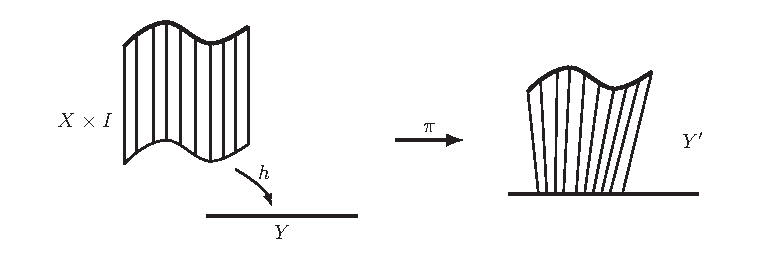
\includegraphics[width=.96\textwidth]{figures/5-6-1.pdf}\\图 5.6.1\end{center}

\sourcepage{337}
若作适当三角剖分，使 $i(X),j(Y)$ 及每个柱 $\pi(\sigma\times I)$ 都为子复形，可把柱分成三类开 $p$ 维胞腔：顶面的 $p$ 维开单形、底面的 $p$ 维开单形，以及中间的 $(p-1)$ 维单形乘开区间。因此胞腔链群正是
\[
C_p(X)\oplus C_p(Y)\oplus C_{p-1}(X).
\]
前两项上边缘分别是原来的边缘。第三类胞腔的边缘由柱的上下两面及侧面组成。粘合后，它具有 $h_\#\sigma-\sigma\pm(\partial\sigma)\times I$ 的形式，写成三元组就是 $(-\sigma,h_\#\sigma,\pm\partial\sigma)$。为使边缘平方为零，末项必须取负号，这恰是代数映射柱的定义。

下面给出一个联系同调与上同调的应用，第七章将推广它。

\entry{定义}{5.6.9}双线性\textbf{取值映射} $\operatorname{Hom}(C_p,G)\times C_p\to G$ 诱导配对
\[
H^p(\mathcal C;G)\times H_p(\mathcal C)\to G,
\]
称为\textbf{Kronecker 指标}（Kronecker index），仍记为 $\langle\alpha^p,\beta_p\rangle$。

\sourcepage{338}
\entry{引理}{5.6.10}Kronecker 指标良定义。

\textbf{证明：}若 $z_p$ 闭、$z^p$ 上闭，则改变代表后的取值为
\begin{align*}
\langle z^p+\delta d^{p-1},z_p+\partial d_{p+1}\rangle
&=\langle z^p,z_p\rangle+\langle d^{p-1},\partial z_p\rangle\\
&\quad+\langle\delta z^p,d_{p+1}\rangle+\langle d^{p-1},\partial^2d_{p+1}\rangle
=\langle z^p,z_p\rangle.
\end{align*}
\hfill$\square$

\entry{定义}{5.6.11}\textbf{Kronecker 映射}
\[
\kappa:H^p(\mathcal C;G)\to\operatorname{Hom}(H_p(\mathcal C),G)
\]
定义为 $(\kappa\alpha)(\beta)=\langle\alpha,\beta\rangle$。由第一变量线性性，它是同态；自然性留作习题 2。

\entry{引理}{5.6.12}若 $\mathcal C$ 自由，则存在自然短正合列
\[
0\leftarrow\operatorname{Hom}(H_p(\mathcal C),G)\xleftarrow{\kappa}H^p(\mathcal C;G)
\leftarrow\ker\kappa\leftarrow0.
\]
它分裂，但分裂不自然。本引理不依赖本节前面的定理。

\textbf{证明：}构造 $\lambda^*$ 使 $\kappa\lambda^*$ 为恒等。由于 $Z_p$ 是 $C_p$ 的直和项，投影 $\pi:Z_p\to H_p(\mathcal C)$ 可延拓为 $\lambda:C_p\to H_p(\mathcal C)$。令 $E_p=H_p(\mathcal C)$，所有边缘为零，则 $H_p(\mathcal E)=E_p$，$H^p(\mathcal E;G)=\operatorname{Hom}(H_p(\mathcal C),G)$。因为 $\lambda$ 在边缘上为零，它是链映射，且在同调上诱导恒等。

\sourcepage{339}
其上同调映射未必为同构，但对任意 $\gamma:H_p(\mathcal C)\to G$ 及闭链 $z_p$，有
\[
(\kappa\lambda^*\gamma)(\{z_p\})=\langle\gamma,\lambda(z_p)\rangle=\gamma(\{z_p\}).
\]
因此复合为恒等，证明分裂与满射性。\hfill$\square$

\entry{定理}{5.6.13}若自由链复形的所有同调群也自由，则 $\kappa$ 在所有维数均为同构。

\textbf{证明：}上一证明中的 $\mathcal E$ 此时自由，且 $\lambda$ 诱导同调同构。由定理 5.6.6，$\lambda^*$ 为同构。因 $\kappa\lambda^*$ 为恒等，$\kappa$ 也是同构。\hfill$\square$

因此，自由同调情形下，上同调自然等于同调的对偶群。第七章将推广这一结论；实际上只需单个 $H_{p-1}(\mathcal C)$ 自由即可。

\subsection*{习题}
\begin{enumerate}
\item 验证引理 5.6.5 的边缘平方为零。
\item \begin{enumerate}[label=(\alph*)]
\item 证明对链映射 $\varphi:\mathcal C\to\mathcal D$，有 $\kappa_{\mathcal C}\varphi^*=\overline{\varphi_*}\kappa_{\mathcal D}$，即 Kronecker 映射自然。
\item 配对在两个变量上变性相反，直接表述自然性较不便。证明 $\langle\varphi^*\alpha,\beta\rangle=\langle\alpha,\varphi_*\beta\rangle$。
\end{enumerate}
\item 设 $H_n(X),H^n(X),H_n(Y),H^n(Y)$ 都为无限循环群，$f:X\to Y$ 连续。若 $f_*$ 为乘以 $d$，证明除符号选择外，$f^*$ 也为乘以 $d$。〔提示：证明 $\kappa$ 为同构。〕
\item 引理 5.6.12 的延拓 $\lambda$ 涉及任意选择，证明分裂确实不自然。
\begin{enumerate}[label=(\alph*)]
\item 找自由链复形及链映射 $\varphi:\mathcal C\to\mathcal D$，使无论怎样选择，两条分裂 $\lambda^*$ 都不能满足 $\varphi^*\lambda_{\mathcal D}^*=\lambda_{\mathcal C}^*\overline{\varphi_*}$。
\item 〔*〕找空间及连续映射，使其奇异链复形实现 (a) 的情形。
\end{enumerate}
\item 求 $\Z/n$ 的一个自由消解。
\end{enumerate}

\section{*自由链复形中的链等价}
\sourcepage{341}
本节结果将在第 7.6、7.10 节证明若干正合列的自然性时使用。我们证明定理 5.6.6 的另一版本：若自由链复形在某一维数以下均为零，则诱导所有维数同调同构的链映射，不仅诱导上同调同构，本身还是链等价。证明使用上一节的代数映射柱。先给出一个稍一般的初等引理，以备以后使用。

\entry{引理}{5.7.1}设 $\mathcal E,\mathcal F$ 为非负链复形，$p>0$ 时 $E_p$ 自由且 $H_p(\mathcal F)=0$。则任意两个零维上相同的链映射 $f,g:\mathcal E\to\mathcal F$ 链同伦。

\textbf{证明：}令 $D:E_0\to F_1$ 为零，则零维已满足 $\partial D+D\partial=g-f$。归纳地，若已在 $p-1$ 维定义 $D$，对 $E_p$ 的每个基元 $e$，表达式 $g(e)-f(e)-D\partial e$ 为闭链。因为 $H_p(\mathcal F)=0$，可选 $D(e)$，使其边缘为该闭链，再线性延拓。\hfill$\square$

这个结果也可由无环载体定理导出，但需仔细处理，不值得为此费力。

\entry{定理}{5.7.2}设自由链复形 $\mathcal C,\mathcal D$ 在某一维数以下均为零。若链映射 $\varphi:\mathcal C\to\mathcal D$ 在所有维数诱导同调同构，则它是链等价。

\textbf{证明：}回到引理 5.6.5 的映射柱 $D'_p=C_p\oplus D_p\oplus C_{p-1}$。包含 $i$ 链同伦于 $j\varphi$，故它也诱导同调同构。于是商复形 $\mathcal E=\mathcal D'/\mathcal C$ 同调为零，且
\[
E_p=D_p\oplus C_{p-1},\qquad\partial(d,c)=(\partial d+\varphi c,-\partial c).
\]
\sourcepage{342}
它自由并在某一维数以下为零，平移维数后可设零维及更低均为零。对其恒等与零映射应用上一个引理，得到收缩同伦 $D:E_p\to E_{p+1}$，满足 $\partial D+D\partial=\operatorname{id}$。所需链映射和同伦都藏在这个公式中。

将其分量记为
\[
D(d,0)=(\theta d,\psi d),\qquad D(0,c)=(\lambda c,\mu c).
\]
在 $(d,0)$ 上展开收缩公式，得
\[
d=\theta\partial d+\partial\theta d+\varphi\psi d,\qquad
0=\psi\partial d-\partial\psi d.
\]
第二式说明 $\psi:\mathcal D\to\mathcal C$ 为链映射，第一式说明 $\theta$ 是 $\varphi\psi$ 到恒等映射的链同伦。

再对 $(0,c)$，计算
\begin{align*}
D\partial(0,c)&=(\theta\varphi c-\lambda\partial c,\psi\varphi c-\mu\partial c),\\
\partial D(0,c)&=(\partial\lambda c+\varphi\mu c,-\partial\mu c).
\end{align*}
比较第二分量，得 $c=\psi\varphi c-\mu\partial c-\partial\mu c$，即 $\mu$ 是恒等映射与 $\psi\varphi$ 之间的链同伦。因此 $\psi$ 是链同伦逆。\hfill$\square$

\sourcepage{343}
\subsection*{习题}
\begin{enumerate}
\item 若 $\mathcal A$ 是空间 $X$ 的子集族，其内部覆盖 $X$，证明包含 $\mathcal S^{\mathcal A}(X)\to\mathcal S(X)$ 是链等价。
\item 证明第 4.7 节的链映射 $\eta:\mathcal C(K)\to\mathcal S(|K|)$ 是链等价。
\item 给出链等价的严格定义。
\end{enumerate}

\section{CW 复形的上同调}
\sourcepage{343}
现在可计算一些熟悉空间的上同调群，并找出代表其生成元的具体上闭链。基本工具如下。

\entry{定理}{5.8.1}若 $X$ 是 CW 复形，$\mathcal D(X)$ 是其胞腔链复形，则对任意 $p,G$，
\[
H^p(\mathcal D(X);G)\cong H^p(X;G).
\]
若 $X$ 可由复形 $K$ 三角剖分，则此同构由包含映射 $\mathcal D(X)\to\mathcal C(K)$ 诱导，方向与链映射相反。

\textbf{证明：}胞腔链复形与奇异链复形都自由，且同调同构，由推论 5.6.7，上同调也同构。可三角剖分时，定理 4.13.9 说明包含映射诱导同调同构，因此也诱导上同调同构。\hfill$\square$

\entry{推论}{5.8.2}设 $n>0$。有 $H^i(S^n;G)\cong G$（$i=0,n$），$H^i(B^n,S^{n-1};G)\cong G$（$i=n$），其余维数均为零。

\textbf{证明：}球面的胞腔链复形仅在零维及 $n$ 维为无限循环群，所有边缘为零，得到第一结论。再由球可缩及约化上同调长正合列，得到第二结论。\hfill$\square$

\sourcepage{344}
\entry{例}{5.8.3}环面 $T$ 与 Klein 瓶 $S$ 的胞腔链复形均具有形式
\[
0\to\Z\xrightarrow{\partial_2}\Z\oplus\Z\xrightarrow{\partial_1}\Z\to0.
\]
取二维生成元 $\gamma$，一维基 $w_1,z_1$。环面的所有边缘均为零，所以
\[
H^2(T;G)\cong G,\qquad H^1(T;G)\cong G\oplus G,\qquad H^0(T;G)\cong G.
\]
Klein 瓶满足 $\partial_1=0$、$\partial_2\gamma=2z_1$。在一维对偶群 $G\oplus G$ 中，第一项是只在 $w_1$ 上可能非零的同态，第二项是只在 $z_1$ 上可能非零的同态。上边缘在第一项上为零，在第二项上为乘以 $2$。因此
\[
H^2(S;G)\cong G/2G,\qquad H^1(S;G)\cong G\oplus\ker(G\xrightarrow{2}G),\qquad H^0(S;G)\cong G.
\]
特别地，整数系数时为 $H^2(S)\cong\Z/2$、$H^1(S)\cong\Z$、$H^0(S)\cong\Z$；模二系数时为 $H^2(S;\Z/2)\cong\Z/2$、$H^1(S;\Z/2)\cong(\Z/2)^2$、$H^0(S;\Z/2)\cong\Z/2$。\translatornote{原书模二公式的最后一项漏写了系数 $\Z/2$。}

一旦知道胞腔链复形，群的计算就不难。但要找出具体的\emph{单纯上闭链}代表生成元，则较困难；下一节计算杯积时将需要它们。

\sourcepage{345}
\begin{center}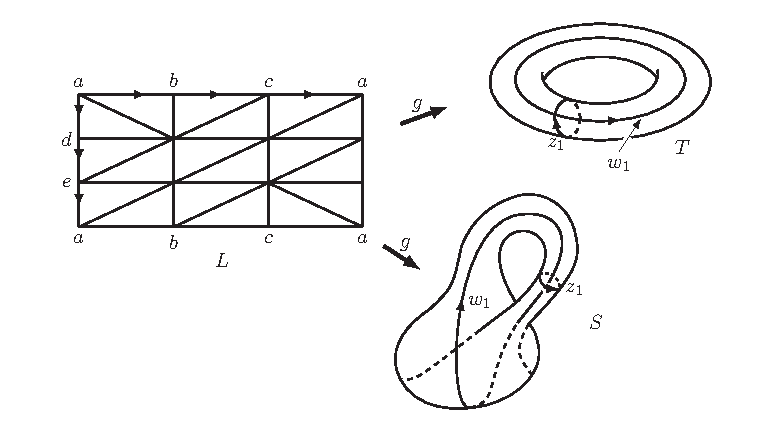
\includegraphics[width=.96\textwidth]{figures/5-8-1.pdf}\\图 5.8.1\end{center}
同调中，生成闭链容易找到：矩形中全部逆时针二维单形之和 $d$ 的像 $\gamma=g_\#d$ 生成 $D_2(X)$；链
\[
w_1=[a,b]+[b,c]+[c,a],\qquad z_1=[a,d]+[d,e]+[e,a]
\]
是 $D_1(X)$ 的基。胞腔同调同构由包含诱导，所以它们作为单纯链仍代表相应同调类。

上同调则不同。定义 $\lambda:D_2(X)\to\Z$ 使 $\lambda(\gamma)=1$；定义 $\varphi,\psi:D_1(X)\to\Z$，使
\[
\langle\varphi,w_1\rangle=1,\quad\langle\varphi,z_1\rangle=0,\qquad
\langle\psi,w_1\rangle=0,\quad\langle\psi,z_1\rangle=1.
\]
环面中，$\lambda$ 生成二维胞腔上同调，$\varphi,\psi$ 为一维基。Klein 瓶中，$\delta\varphi=0$、$\delta\psi=2\lambda$，故 $\lambda$ 代表二维非零类，$\varphi$ 代表一维生成元。

\sourcepage{346}
这些定义域只是胞腔链群，不能直接视为整个单纯复形上的上闭链，因为包含 $i:D_p(X)\to C_p(X)$ 的对偶是反向的限制映射。必须找到定义于所有单纯链上的上闭链，限制后等于 $\lambda,\varphi,\psi$，或代表它们的上同调类。一般没有现成的寻找程序；本例借助“栅栏”的直观可以找到。

\entry{例}{5.8.4（环面上同调的生成元）}图 5.8.2 中的上链 $w^1,z^1$ 直接计算可知上闭，且
\[
\langle w^1,w_1\rangle=1,\quad\langle w^1,z_1\rangle=0,\qquad
\langle z^1,w_1\rangle=0,\quad\langle z^1,z_1\rangle=1.
\]
所以它们限制后分别为 $\varphi,\psi$，代表 $H^1(T)$ 的一组基。任取逆时针定向二维单形 $\sigma$，则 $\sigma^*$ 上闭，且 $\langle\sigma^*,\gamma\rangle=1$，故限制为 $\lambda$，代表 $H^2(T)$ 的生成元。更一般地，$\sum n_i\sigma_i^*$ 的限制为 $\lambda$ 当且仅当 $\sum n_i=1$。

\sourcepage{347}
\begin{center}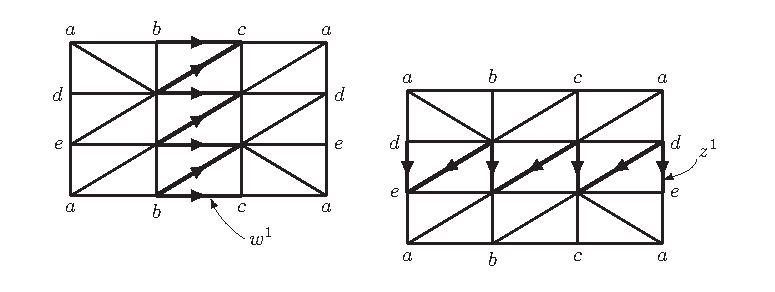
\includegraphics[width=.96\textwidth]{figures/5-8-2.pdf}\\图 5.8.2\end{center}
\entry{例}{5.8.5（Klein 瓶的整数上同调生成元）}交换图 5.8.2 中表示 $w^1$ 的矩形右侧标号 $d,e$，得到图 5.8.3。上链 $w^1$ 仍上闭，并生成 $H^1(S)$。任一二维初等上链 $\sigma^*$ 代表 $H^2(S)$ 的非零类。更一般地，若沿矩形全部二维单形取逆时针定向，则 $\sum n_i\sigma_i^*$ 代表非零类当且仅当系数和为奇数。
\begin{center}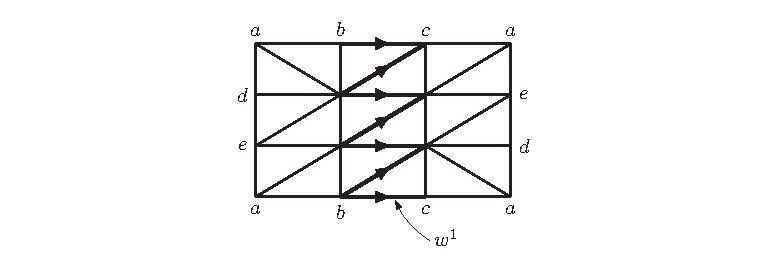
\includegraphics[width=.96\textwidth]{figures/5-8-3.pdf}\\图 5.8.3\end{center}

\entry{例}{5.8.6（Klein 瓶的模二上同调生成元）}按照同样论证，图 5.8.4 的 $w^1,z^1$ 生成二维向量空间 $H^1(S;\Z/2)$。图中不画箭头，因为模二时 $1=-1$。任一 $\sigma^*$，或奇数个不同初等二维上链之和，生成 $H^2(S;\Z/2)$。

\sourcepage{348}
\begin{center}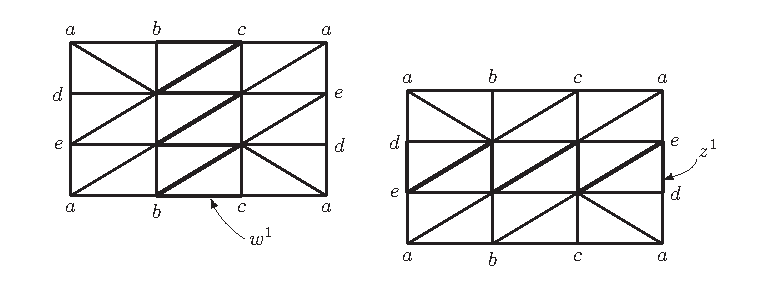
\includegraphics[width=.96\textwidth]{figures/5-8-4.pdf}\\图 5.8.4\end{center}
\entry{例}{5.8.7（实射影平面的模二上同调）}$H^i(P^2;\Z/2)\cong\Z/2$，$i=0,1,2$。二维初等上链代表二维生成元。图 5.8.5 的一维上闭链在胞腔生成闭链
\[
[a,b]+[b,c]+[c,d]+[d,e]+[e,f]+[f,a]
\]
上取值为 $1$，所以代表 $H^1(P^2;\Z/2)$ 的生成元。
\begin{center}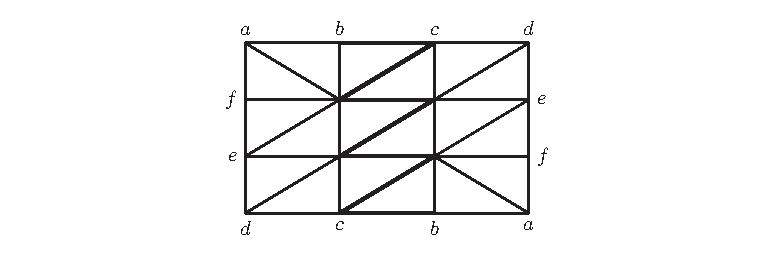
\includegraphics[width=.96\textwidth]{figures/5-8-5.pdf}\\图 5.8.5\end{center}

\sourcepage{349}
\subsection*{习题}
\begin{enumerate}
\item 分别用整数、模二、有理系数计算 $P^n,P^\infty$ 的上同调。
\item 计算 $\mathbb CP^n,\mathbb CP^\infty$ 的上同调。
\item 计算 $H^i(T\#T)$；采用第 1.7 节习题的三角剖分，找出生成上同调的单纯上闭链。
\item 计算四个实射影平面连通和的模二上同调，并找出生成上闭链。
\item 计算 Klein 瓶的 $\Z/6$ 系数上同调，仿照例 5.8.5、5.8.6 找代表上闭链。
\item 计算五重愚人帽的整数及 $\Z/5$ 系数上同调（第 1.7 节习题 6），三角剖分后找生成上闭链。
\item 计算 $L(n,k)$ 的整数及 $\Z/n$ 系数上同调。
\item 三角剖分 $S^2,T$，设 $f:T\to S^2$ 单纯。若 $f_*:H_2(T)\to H_2(S^2)$ 为乘以 $d$，通过比较生成元上取值，证明 $f^*:H^2(S^2)\to H^2(T)$ 也为乘以 $d$。与第 5.6 节习题 3 比较。
\item 计算环面的 $\Z/6$ 系数上同调。
\end{enumerate}

\section{杯积}
\sourcepage{349--350}
第 5.6 节说明：同调群若不能区分两个空间，上同调群也不能。那为什么还研究上同调？有多个答案：它自然出现在映射的同伦分类中，也出现在流形上微分形式的积分中。本节给出另一个答案：上同调群还有额外的\emph{环结构}，这种结构能区分仅靠群无法区分的空间。

我们用具体的上链公式定义乘法，这也是历史上最初的途径。公式由 Alexander、\v Cech、Whitney 约在 1936 年发现，当时显得很神秘，几何意义不清，也不明白为什么一般空间的上同调有乘法而同调没有。

紧可定向流形的同调早已知道有称为\textbf{交积}的乘法，几何意义明确，但推广到一般空间的尝试未能成功。直到 1942 年 Lefschetz 给出新的上同调乘法定义，才说明一般空间为什么有上同调环而没有相应同调环。同时，Poincar\'e 对偶说明两种环在都存在时同构。第 7.11、8.9 节将回到这些问题。

\subsection*{环、模和域的回顾}
环 $R$ 是带乘法的加法阿贝尔群，乘法满足结合律与左右分配律；通常先乘后加。若乘法交换，称为交换环。若有元素 $1$ 满足 $1\alpha=\alpha1=\alpha$，称为单位元，它唯一，且 $(-1)\alpha=-\alpha$、$0\alpha=0$。若非零交换含幺环中每个非零元均有乘法逆，则称为域。

\entry{例}{5.9.1}环的例子包括 $\Z$、$\Z/n$、整数系数方阵环、整数系数多项式环。域的例子包括素数 $p$ 对应的 $\Z/p$，以及 $\mathbb Q,\R,\mathbb C$。

\sourcepage{351}
若加法阿贝尔群 $A$ 配有标量乘法 $R\times A\to A$，满足
\[
\alpha(a+b)=\alpha a+\alpha b,\quad(\alpha+\beta)a=\alpha a+\beta a,\quad
\alpha(\beta a)=(\alpha\beta)a,\quad1a=a,
\]
称为 $R$ 模。模同态是满足 $\varphi(\alpha a)=\alpha\varphi(a)$ 的群同态；核与余核自然也是模。若 $R=F$ 为域，则模称为 $F$ 上的向量空间，模同态称为线性变换。本书较少讨论一般模，主要使用环和向量空间。

\entry{例}{5.9.2}$R$ 本身及 $R^n$ 自然为 $R$ 模，后者按坐标作标量乘法。

\entry{例}{5.9.3}每个阿贝尔群都是自然的 $\Z$ 模，正整数作用为重复相加，其他整数按通常方式定义。

\subsection*{杯积}
本节及下一节始终假设 $R$ 为交换含幺环。

\entry{定义}{5.9.4}记奇异上链群 $S^p(X;R)=\operatorname{Hom}(S_p(X),R)$。定义
\[
\smile:S^p(X;R)\times S^q(X;R)\to S^{p+q}(X;R),
\]
使对每个奇异 $(p+q)$ 维单形 $T$ 有
\[
\begin{split}
\langle c^p\smile c^q,T\rangle
={}&\langle c^p,T\circ\ell(\epsilon_0,\ldots,\epsilon_p)\rangle\\
&\cdot\langle c^q,T\circ\ell(\epsilon_p,\ldots,\epsilon_{p+q})\rangle.
\end{split}\tag{*}
\]
称为上链的\textbf{杯积}（cup product）。\translatornote{原书此处把 Hom 所定义的群称为奇异“链”群，应为上链群。}

\sourcepage{352}
第一个限制可称为 $T$ 的“前 $p$ 维面”，第二个为“后 $q$ 维面”；它们共用顶点 $\epsilon_p$。右端是系数环中的乘法。这个看似神秘的公式意味着什么，还有待说明。

\entry{定理}{5.9.5}上链杯积双线性、结合。在每个零维奇异单形上取 $1$ 的上链 $z^0$ 是单位元，且
\[
\delta(c^p\smile c^q)=(\delta c^p)\smile c^q+(-1)^pc^p\smile\delta c^q.
\]
\textbf{证明：}双线性由系数环分配律立即得到。结合律可对一个 $(p+q+r)$ 维单形取值验证：两种结合方式都得到在依次三段面 $[0,\ldots,p]$、$[p,\ldots,p+q]$、$[p+q,\ldots,p+q+r]$ 上取值的乘积。单位元性质直接来自定义。

验证上边缘公式，令 $r=p+q+1$，对 $T:\Delta_r\to X$ 取值。为缩短公式，记 $T[i_0,\ldots,i_s]=T\circ\ell(\epsilon_{i_0},\ldots,\epsilon_{i_s})$。第一项的值为
\[
\sum_{i=0}^{p+1}(-1)^i\langle c^p,T[0,\ldots,\widehat i,\ldots,p+1]\rangle
\langle c^q,T[p+1,\ldots,r]\rangle;
\]
第二项的值为
\[
(-1)^p\sum_{i=0}^{q+1}(-1)^i\langle c^p,T[0,\ldots,p]\rangle
\langle c^q,T[p,\ldots,\widehat{p+i},\ldots,r]\rangle.
\]
第一和的最后一项与第二和的第一项，除符号 $(-1)^{p+1}$、$(-1)^p$ 外完全相同，故抵消；其余恰是 $\langle c^p\smile c^q,\partial T\rangle$。\hfill$\square$

\sourcepage{353}
\entry{定理}{5.9.6}杯积诱导双线性、结合的运算 $H^p(X;R)\times H^q(X;R)\to H^{p+q}(X;R)$，以 $\{z^0\}$ 为单位元。

\textbf{证明：}两个上闭链之积由上边缘公式仍上闭。改变代表后，
\begin{align*}
&(z^p+\delta d^{p-1})\smile(z^q+\delta d^{q-1})-z^p\smile z^q\\
&\quad=(-1)^p\delta(z^p\smile d^{q-1})
+\delta(d^{p-1}\smile z^q)+\delta(d^{p-1}\smile\delta d^{q-1}),
\end{align*}
所以只改变一个上边缘，运算良定义。其余性质从上链层次继承。\hfill$\square$

\entry{定理}{5.9.7}连续映射 $h:X\to Y$ 诱导的 $h^*$ 保持杯积。

\textbf{证明：}实际上 $h^\#$ 已保持杯积。对 $T$ 取值，$h^\#(c^p\smile c^q)$ 是把杯积公式用于 $h\circ T$；而 $(h^\#c^p)\smile(h^\#c^q)$ 在两个面上的取值也是将 $h\circ T$ 限制到同样两面，所以相等。\hfill$\square$

\entry{定义}{5.9.8}外直和 $H^*(X;R)=\bigoplus_iH^i(X;R)$ 连同杯积组成含幺环，称为 $X$ 的\textbf{上同调环}。杯积对每个变量还是 $R$ 模同态（习题 4），因而它是一个具有 $R$ 算子作用的环。若 $R=F$ 是域，则称为 $F$ 上的\textbf{代数}。

连续映射诱导环同态，同伦等价诱导环同构。因此上同调环是拓扑不变量，事实上是同伦类型不变量。

\sourcepage{354}
\subsection*{交换性}
上同调环一般不按通常意义交换，而满足\textbf{分次交换律}，原书亦称反交换性：
\[
\alpha^p\smile\beta^q=(-1)^{pq}\beta^q\smile\alpha^p.
\]
此时先不证明；后面给出杯积的另一种定义后，证明会容易得多。下一节将计算具体环结构，先给出几种推广。

\subsection*{一般系数的杯积}
若 $G$ 为任意阿贝尔群，同一公式可定义 $S^p(X)\times S^q(X;G)\to S^{p+q}(X;G)$，其中第一因子为整数系数，右端乘法解释为整数对 $G$ 的作用。它双线性；当三个因子的系数依次为 $\Z,\Z,G$ 时满足结合律。$z^0$ 是左单位元。上边缘公式、自然性及上同调层次的良定义性证明不变，因此有
\[
H^p(X)\times H^q(X;G)\to H^{p+q}(X;G).
\]
最一般的常见形式始于一个双线性\textbf{系数配对} $\alpha:G\times G'\to G''$，用它代替系数乘法，得到 $H^p(X;G)\times H^q(X;G')\to H^{p+q}(X;G'')$。本书不需要如此一般。

\sourcepage{355}
\subsection*{相对杯积}
相同公式也定义
\[
H^p(X,A;R)\times H^q(X;R)\to H^{p+q}(X,A;R),
\]
以及两因子都相对 $A$ 的版本，后者是前者的限制。因为若第一因子在 $A$ 的单形上为零，乘积在 $A$ 的单形上也为零。上边缘公式仍成立，所以诱导上同调运算；双线性、结合性和自然性直接继承。第一种运算以绝对零维类 $\{z^0\}$ 为右单位元。

更一般地，若 $\{A,B\}$ 为可切除对，可定义
\[
H^p(X,A;R)\times H^q(X,B;R)\to H^{p+q}(X,A\cup B;R),
\]
见习题。

\subsection*{习题}
\begin{enumerate}
\item 设 $A$ 为 $X$ 的一个道路分支，$B\ne\varnothing$ 为其余分支之并。令 $c^0$ 在像属于 $A$ 的零维单形上取 $1$，其余取 $0$。证明它上闭，并描述对一般 $\beta^p$ 的 $\{c^0\}\smile\beta^p$。
\item 设 $i:A\to X$，$\eta\in H^q(X;R)$，记 $\eta|_A=i^*\eta$。证明将空间偶长正合列
\[
H^{p+1}(X,A)\leftarrow H^p(A)\leftarrow H^p(X)\leftarrow H^p(X,A)
\]
的各项分别右乘 $\eta$ 或 $\eta|_A$，得到映到相应升高 $q$ 维的长正合列的交换图。若全改为左乘，会怎样？
\item 若 $\{A,B\}$ 可切除，证明杯积公式诱导上述最一般的相对杯积，并解释结合律在这里的含义。
\item \begin{enumerate}[label=(\alph*)]
\item 定义 $(\alpha\varphi)(g)=\alpha\varphi(g)$，证明 $\operatorname{Hom}(G,R)$ 自然为 $R$ 模；群同态的对偶为模同态。
\item 依此给 $S^p(X;R)$ 赋模结构，证明 $\delta$ 为模同态，所以 $H^p(X;R)$ 也是模。
\item 证明连续映射诱导的 $h^*$ 为模同态。
\item 证明杯积对每个变量分别为模同态。因此 $H^*(X;R)$ 为带 $R$ 作用的环，域系数时为代数。
\end{enumerate}
\item 给出数学中自然出现的三个代数的例子。
\end{enumerate}

\section{曲面的上同调环}
\sourcepage{356--357}
即使 $X$ 是 CW 复形，也没有计算其奇异上同调环的一般程序：胞腔链复形并不能确定环结构。两个空间可能有同构的胞腔链复形，却有不同构的上同调环。因此，我们转向单纯上同调，给出对应于奇异杯积的公式，再计算若干例子。

\entry{定义}{5.10.1}选取顶点偏序，使每个单形的顶点全序。定义单纯上链的杯积，使 $v_0<\cdots<v_{p+q}$ 时
\[
\langle c^p\smile c^q,[v_0,\ldots,v_{p+q}]\rangle
=\langle c^p,[v_0,\ldots,v_p]\rangle\langle c^q,[v_p,\ldots,v_{p+q}]\rangle.
\]
它与奇异公式十分相似。

\entry{定理}{5.10.2}给定排序后，单纯杯积双线性、结合，以每个顶点上取值 $1$ 的 $z^0$ 为单位，且满足上边缘公式
\[
\delta(c^p\smile c^q)=\delta c^p\smile c^q+(-1)^pc^p\smile\delta c^q.
\]
由该排序定义的链映射 $\eta$ 的对偶，将奇异杯积映为单纯杯积。

\textbf{证明：}各项直接验证；上边缘公式可重复定理 5.9.5 的计算，只改记号。另一证明是：$\eta$ 单射且将基元映为基元，像为直和项，所以其对偶满射。将给定单纯上链延拓为奇异上链，利用奇异公式，再用对偶保持杯积及上边缘，即得单纯公式。\hfill$\square$

\entry{定理}{5.10.3}单纯杯积诱导双线性、结合的上同调运算，不依赖顶点排序，以 $\{z^0\}$ 为单位，并被连续映射诱导的同态保持。

\textbf{证明：}由上边缘公式如前得良定义性。$\eta^*$ 是保持杯积的奇异到单纯上同调同构，且不依赖排序，所以单纯杯积也不依赖排序。它与连续映射诱导的同态可交换，而奇异上同调中的自然性已证，故得结论。\hfill$\square$

\sourcepage{358}
但单纯映射 $f$ 的上链映射 $f^\#$ 未必在\emph{上链层次}保持杯积，因为 $f$ 未必保持顶点排序。若只在有向单纯理论内部工作，这会使自然性证明相当困难。

整数与一般系数配对的杯积，以及相对子复形的杯积，也都存在。相对版本反而更容易：若两个因子分别在 $A,B$ 上为零，其积在 $A\cup B$ 上为零，因为并复形的每个单形必须属于其中之一。此时两子空间本来就是可切除对，奇异版本也有定义。

\entry{定义}{5.10.4}若任意两个正维上同调类之积均为零，称上同调环\textbf{平凡}。这不表示所有乘法为零，因为零维单位元的作用始终存在。

\entry{例}{5.10.5}取环面 $T$ 及图 5.10.1 的上闭链 $w^1,z^1$。记 $\alpha=\{w^1\}$、$\beta=\{z^1\}$，它们生成 $H^1(T)$；任一逆时针二维单形的初等上链之类记为 $\Lambda$，生成 $H^2(T)$。
\begin{center}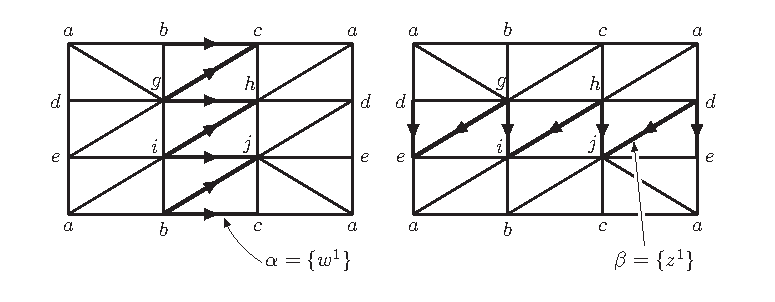
\includegraphics[width=.96\textwidth]{figures/5-10-1.pdf}\\图 5.10.1\end{center}
按字母顺序排列顶点。一个二维单形只有同时有面落在两个上链的载体中时，乘积才可能非零，因此只需考察 $[g,h,i]$、$[h,i,j]$。直接计算
\begin{align*}
\langle w^1\smile z^1,[g,h,i]\rangle&=1\cdot1=1,\\
\langle w^1\smile z^1,[h,i,j]\rangle&=(-1)\cdot0=0.
\end{align*}
故 $w^1\smile z^1=[g,h,i]^*$。这个单形顺时针定向，所以 $\alpha\smile\beta=-\Lambda$。

\sourcepage{359}
反向相乘时，两项分别为 $0\cdot(-1)=0$、$1\cdot1=1$，故 $z^1\smile w^1=[h,i,j]^*$，得到 $\beta\smile\alpha=\Lambda$，符合分次交换律。

直接计算还可得 $\alpha^2=\beta^2=0$。也可把 $w^1$ 换为与它上同调的图 5.10.2 中的 $y^1$，其载体与原栅栏分开，没有二维单形同时碰到两者，故 $w^1\smile y^1=0$。另一证明利用 $\alpha^2=-\alpha^2$，而 $H^2(T)$ 无二阶元素，所以平方为零。
\begin{center}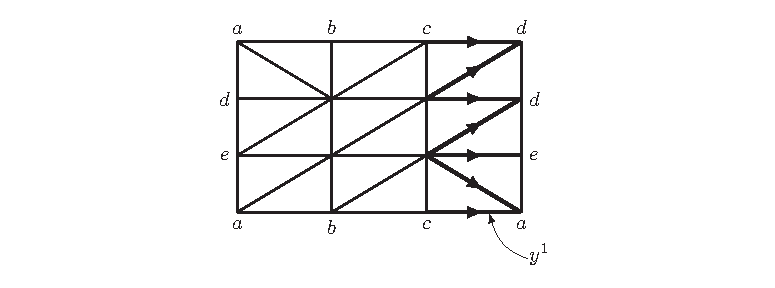
\includegraphics[width=.96\textwidth]{figures/5-10-2.pdf}\\图 5.10.2\end{center}
省略单位元，乘法表为
\[
\begin{array}{c|ccc}
\smile&\alpha&\beta&\Lambda\\\hline
\alpha&0&-\Lambda&0\\
\beta&\Lambda&0&0\\
\Lambda&0&0&0
\end{array}
\]
最后一行、一列因维数原因均为零。

\sourcepage{360}
\entry{例}{5.10.6}计算 Klein 瓶 $S$ 的模二上同调环。仍用 $\alpha=\{w^1\}$、$\beta=\{z^1\}$、$\Lambda=\{\sigma^*\}$，代表如图 5.10.3。上例的部分计算模二后仍成立：$\alpha\beta=\Lambda$，$\alpha^2=0$，后者可借助图 5.10.4 中的 $y^1$。
\begin{center}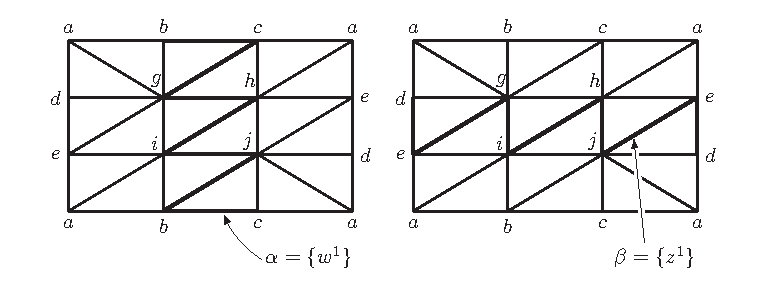
\includegraphics[width=.96\textwidth]{figures/5-10-3.pdf}\\图 5.10.3\end{center}
但 $z^1$ 不能像前者那样从自身移开，必须直接计算其平方。它在 $[d,e,g]$、$[e,g,i]$、$[d,e,j]$ 上取 $1$，其余为零，所以其类为 $3\Lambda=\Lambda$，即 $\beta^2=\Lambda$。

\sourcepage{361}
\begin{center}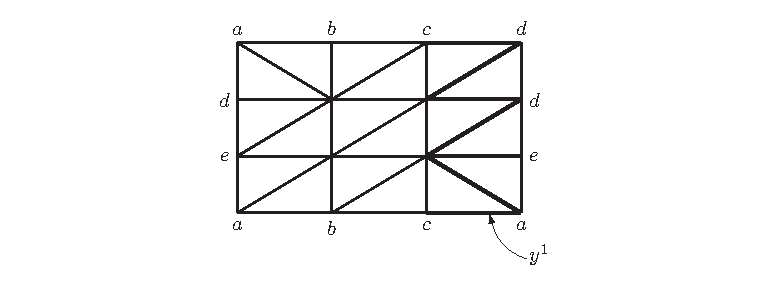
\includegraphics[width=.96\textwidth]{figures/5-10-4.pdf}\\图 5.10.4\end{center}
于是乘法表为
\[
\begin{array}{c|ccc}
\smile&\alpha&\beta&\Lambda\\\hline
\alpha&0&\Lambda&0\\
\beta&\Lambda&\Lambda&0\\
\Lambda&0&0&0
\end{array}
\]

\entry{例}{5.10.7}再计算 $P^2\#P^2$ 的模二上同调环。图 5.10.5 给出一个零维胞腔、两个一维胞腔及一个二维胞腔。取一维基本闭链
\[
w_1=[a,b]+[b,c]+[c,a],\qquad z_1=[a,d]+[d,e]+[e,a],
\]
二维基本链 $\gamma$ 为所有逆时针二维单形之和。它们满足 $\partial w_1=\partial z_1=0$、$\partial\gamma=-2w_1-2z_1$，故模二对偶的所有上边缘为零。因此 $H^1\cong(\Z/2)^2$、$H^2\cong\Z/2$。

图中的 $w^1,z^1$ 在上述两个基本闭链上的取值构成单位矩阵，所以其类 $\epsilon,\zeta$ 为一维上同调基。记二维生成元为 $\Lambda$。

\sourcepage{362}
\begin{center}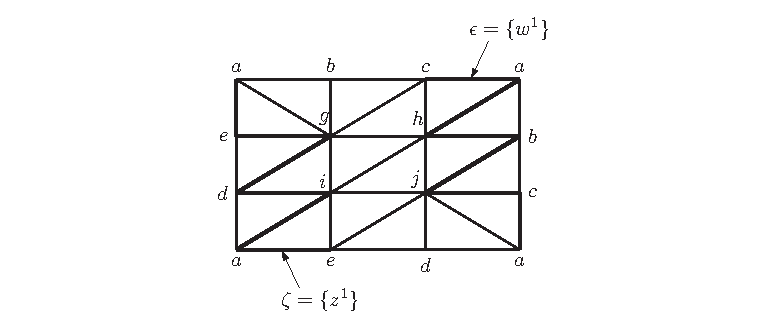
\includegraphics[width=.96\textwidth]{figures/5-10-5.pdf}\\图 5.10.5\end{center}
直接计算得到 $w^1\smile z^1=0$、$w^1\smile w^1=[a,c,j]^*$、$z^1\smile z^1=[a,e,g]^*$。因此
\[
\begin{array}{c|ccc}
\smile&\epsilon&\zeta&\Lambda\\\hline
\epsilon&\Lambda&0&0\\
\zeta&0&\Lambda&0\\
\Lambda&0&0&0
\end{array}
\]
然而 $P^2\#P^2$ 同胚于 Klein 瓶，所以这个环与上一例同构，虽然乘法表看起来很不一样。构造同构留给读者。这说明仅看不同基下的乘法表，通常不能立刻判断两个环是否同构。

\entry{例}{5.10.8}取图 5.10.6 的 $X=S^1\vee S^1\vee S^2$，即两个圆周与一个球面共用一点的\textbf{楔和}（wedge product）。它同样有零维一个、二维一个、一维两个胞腔，基本链为
\[
w_1=[a,b]+[b,c]+[c,a],\quad z_1=[a,d]+[d,e]+[e,a],\quad z_2=\partial[a,f,g,h].
\]
所有胞腔边缘为零，所以它与环面具有同构的胞腔链复形、同调群和上同调群。

\sourcepage{363}
\begin{center}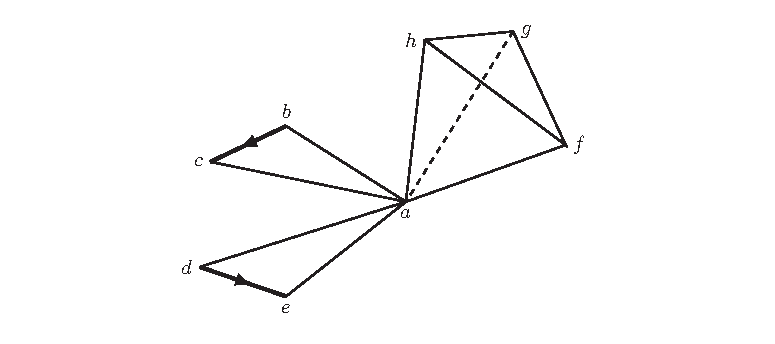
\includegraphics[width=.96\textwidth]{figures/5-10-6.pdf}\\图 5.10.6\end{center}
但上同调环不同。上闭链 $w^1=[b,c]^*$、$z^1=[d,e]^*$ 限制后为胞腔上链群的一组对偶基；没有二维单形具有其载体中的边，所以这些生成元之间的杯积全为零，环平凡。而环面的环不平凡。

这些例子说明杯积通常不易计算，困难在于必须进入单纯层次，找到具体上闭链代表。任何提供一般杯积信息的定理都很有价值。以后将证明两个这样的定理：一个描述乘积空间的上同调环，另一个描述流形的上同调环，特别能用于计算射影空间。

\sourcepage{364--365}
\subsection*{习题}
以下 $T$ 表示环面，$S$ 表示 Klein 瓶。
\begin{enumerate}
\item 若 $f:S^2\to T$ 连续，证明 $f^*:H^2(T)\to H^2(S^2)$ 为零，从而 $f_*:H_2(S^2)\to H_2(T)$ 为零。对 $g:T\to S^2$ 能说什么？
\item 证明下列情形中 $f^*:H^2(Y;\Z/2)\to H^2(X;\Z/2)$ 为零：$X=S^2,Y=S$；$X=S,Y=T$；$X=T,Y=S$。
\item 写出下列环的乘法表：$n$ 重环面连通和的整数上同调环；$P^2$ 的模二上同调环；$n$ 重实射影平面连通和的模二上同调环。
\item 构造例 5.10.6 与例 5.10.7 两个环之间的同构。\translatornote{原书此题引为例 5.10.5 与 5.10.6，但这两例的系数及群均不同，不可能同构；按前文留作习题的说明，应指后两例。}
\item 比较 Klein 瓶与 $P^2\vee S^1$。
\begin{enumerate}[label=(\alph*)]
\item 证明整数上同调环同构。
\item 证明模二上同调环不同构。注意仅给出不同乘法表还不足以证明。
\end{enumerate}
\item 计算三重愚人帽的模三上同调环。
\item \begin{enumerate}[label=(\alph*)]
\item 对 Möbius 带及其边界 $(M,E)$，计算模二相对与绝对上同调之间的杯积，以及两个相对因子之间的杯积。
\item 对圆柱面 $M=S^1\times I$、$E=S^1\times\Bd I$ 重复 (a)。
\end{enumerate}
\begin{center}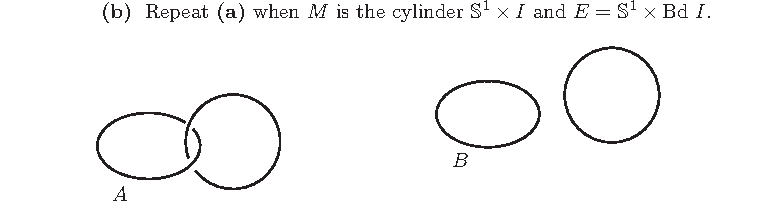
\includegraphics[width=.96\textwidth]{figures/5-10-7.pdf}\\图 5.10.7\end{center}
\item 设 $A$ 为 $S^3$ 中两个一次套链的圆周之并，$B$ 为两个不套链的圆周之并，见图 5.10.7。证明它们补空间的上同调群同构，但上同调环不同构。
\item 对上一题的同调能说什么？
\end{enumerate}

\chapter{带系数的同调}
\section{引言}
\sourcepage{366}
研究任意系数的上同调后，现在回到第一章单纯理论中曾简要介绍的主题：任意系数的同调。

首先引入称为张量积的代数函子，并研究其性质。它在同调论中的作用，类似 Hom 函子在上同调论中的作用。随后研究任意系数同调。

\section{张量积}
\sourcepage{366--367}
对阿贝尔群 $A,B$，常考虑从直积 $A\times B$ 到第三个群的同态。但有时更重要的是\textbf{双线性映射}，即对每个变量分别为同态的映射。本节构造群 $A\otimes B$，使从它出发的同态自然对应于从 $A\times B$ 出发的双线性映射，将后者的研究化为熟悉的同态问题。

\entry{定义}{6.2.1}令 $F(A,B)$ 为以集合 $A\times B$ 为自由基的阿贝尔群，令\textbf{关系子群} $R(A,B)$ 由所有
\[
(a+a',b)-(a,b)-(a',b),\qquad(a,b+b')-(a,b)-(a,b')
\]
生成。定义\textbf{张量积}（tensor product）$A\otimes B=F(A,B)/R(A,B)$，以 $a\otimes b$ 表示 $(a,b)$ 的陪集。

任意集合映射 $A\times B\to C$ 唯一延拓为自由群上的同态；它双线性，当且仅当延拓在关系子群上为零。因此从张量积到 $C$ 的同态，与上述双线性映射一一对应。

每个张量积元素都是有限个 $a\otimes b$ 的整数线性组合。注意一般元素未必是单个纯张量；纯张量是生成元。定义给出
\[
(a+a')\otimes b=a\otimes b+a'\otimes b,\qquad
a\otimes(b+b')=a\otimes b+a\otimes b'.
\]
由 $a\otimes b=(0+a)\otimes b$ 可得 $0\otimes b=0$，同理 $a\otimes0=0$。进而
\[
(-a)\otimes b=-(a\otimes b)=a\otimes(-b),\qquad
(na)\otimes b=n(a\otimes b)=a\otimes(nb)
\]
对所有整数 $n$ 成立。

\entry{定义}{6.2.2}同态 $f:A\to A'$、$g:B\to B'$ 诱导唯一同态 $f\otimes g:A\otimes B\to A'\otimes B'$，使 $(f\otimes g)(a\otimes b)=f(a)\otimes g(b)$。它来自明显的双线性映射，称为两个同态的张量积。

\entry{引理}{6.2.3}上述对象与态射的对应构成从成对阿贝尔群范畴到阿贝尔群范畴的协变函子。验证留给读者。

\sourcepage{368}
\entry{定理}{6.2.4}存在自然同构 $\Z\otimes G\cong G$，将 $n\otimes g$ 映为 $ng$。

\textbf{证明：}整数作用是双线性映射，故诱导 $\varphi:\Z\otimes G\to G$。令 $\psi(g)=1\otimes g$，则 $\varphi\psi(g)=g$，且 $\psi\varphi(n\otimes g)=1\otimes ng=n\otimes g$，所以互逆。对 $f:G\to H$，两条路径都将 $n\otimes g$ 映为 $nf(g)$，证明自然性。\hfill$\square$

须警惕：子群的张量积未必是原群张量积的子群。虽然包含映射诱导 $A'\otimes B'\to A\otimes B$，它可能不单射。例如 $\mathbb Q\otimes\Z/2=0$，因为 $a\otimes b=(a/2)\otimes2b=0$；但 $\Z\otimes\Z/2\cong\Z/2\ne0$。与单射不同，满射的张量积总满射。

\sourcepage{369}
\entry{引理}{6.2.5}若 $\varphi:B\to C$、$\varphi':B'\to C'$ 满射，则 $\varphi\otimes\varphi'$ 满射，其核由所有满足 $b\in\ker\varphi$ 或 $b'\in\ker\varphi'$ 的 $b\otimes b'$ 生成。

\textbf{证明：}记所述子群为 $G$。映射在它上面为零，诱导 $\Phi:(B\otimes B')/G\to C\otimes C'$。给定 $c,c'$，选原像 $b,b'$，定义 $\psi(c,c')=b\otimes b'+G$。若另选 $b_0,b'_0$，差为
\[
(b-b_0)\otimes b'+b_0\otimes(b'-b'_0)\in G,
\]
故良定义。它双线性，诱导 $\Psi$，并在生成元上直接可见 $\Phi\Psi,\Psi\Phi$ 都为恒等，证明结论。\hfill$\square$

\entry{定理}{6.2.6}若 $A\xrightarrow{\varphi}B\xrightarrow{\psi}C\to0$ 正合，则
\[
A\otimes G\xrightarrow{\varphi\otimes i_G}B\otimes G\xrightarrow{\psi\otimes i_G}C\otimes G\to0
\]
正合。若原列还在左侧单射且分裂，则张量后的列也单射且分裂。

\textbf{证明：}上一引理说明第二个映射满射，其核由 $b\otimes g$（$b\in\ker\psi$）生成；第一个映射的像由 $\varphi(a)\otimes g$ 生成。因为 $\ker\psi=\operatorname{im}\varphi$，核像相等。若有 $p\varphi=i_A$，则 $(p\otimes i_G)(\varphi\otimes i_G)=i_{A\otimes G}$，给出单射与分裂。\hfill$\square$

\sourcepage{370}
\entry{推论}{6.2.7}存在自然同构 $\Z/m\otimes G\cong G/mG$。

\textbf{证明：}对 $\Z\xrightarrow{m}\Z\to\Z/m\to0$ 张量 $G$，再用 $\Z\otimes G\cong G$，得 $G\xrightarrow{m}G\to\Z/m\otimes G\to0$，结论随即成立。\hfill$\square$

\entry{定理}{6.2.8}存在自然同构：
\begin{enumerate}[label=(\alph*)]
\item $A\otimes B\cong B\otimes A$；
\item $(\bigoplus A_\alpha)\otimes B\cong\bigoplus(A_\alpha\otimes B)$；
\item $A\otimes(\bigoplus B_\alpha)\cong\bigoplus(A\otimes B_\alpha)$；
\item $A\otimes(B\otimes C)\cong(A\otimes B)\otimes C$。
\end{enumerate}
\textbf{证明：}(a) 交换两个坐标诱导自由群同构，并把关系子群映为关系子群。

(b) 取直和的包含 $j_\alpha$ 与投影 $\pi_\alpha$。张量后得到 $f_\alpha=j_\alpha\otimes i_B$、$g_\alpha=\pi_\alpha\otimes i_B$，满足 $g_\beta f_\alpha=0$（$\alpha\ne\beta$）、$g_\alpha f_\alpha=i$。任一生成元 $a\otimes b$ 中，$a$ 只有有限个直和分量，故它是诸 $f_\alpha$ 的像的有限和。引理 1.5.1 遂给出直和分解。

\sourcepage{371}
(c) 由 (a)、(b) 得到。

(d) 从任一种结合方式的张量积到群 $G$ 的同态，都恰对应于 $A\times B\times C\to G$ 中对每个变量分别线性的映射，称为\textbf{多线性映射}。具体地，$a\otimes(b\otimes c)$ 与 $(a\otimes b)\otimes c$ 这两个多线性表达式分别诱导双向同态；复合在生成元上为恒等，故互逆。自然性留给读者验证。\hfill$\square$

\entry{推论}{6.2.9}若 $0\to A\to B\to C\to0$ 正合且 $G$ 无挠，则张量 $G$ 后仍为短正合列。

\textbf{证明：步骤 1。}若 $G$ 自由，因 $D\otimes\Z\cong D$，张量后序列是原正合列的若干份直和，故正合。

\textbf{步骤 2。}先证有限性事实：若 $\sum a_i\otimes b_i=0$，则有有限生成子群 $A_0\subset A$、$B_0\subset B$，包含这些元素，使该和在 $A_0\otimes B_0$ 中已为零。因为自由群中 $\sum(a_i,b_i)$ 属于关系子群，它是有限个关系生成元的有限整数线性组合。把这些关系中出现的所有第一、第二坐标分别加入生成集，即得到所求 $A_0,B_0$。

\sourcepage{372}
\textbf{步骤 3。}由右正合性只需证明左侧单射。若 $\sum a_i\otimes g_i$ 映为零，则 $\sum\varphi(a_i)\otimes g_i=0$。由步骤 2，存在有限生成的 $B_0\subset B$、$G_0\subset G$，使它已在 $B_0\otimes G_0$ 中为零，因而在 $B\otimes G_0$ 中为零。群 $G_0$ 有限生成且无挠，故自由。由步骤 1，$A\otimes G_0\to B\otimes G_0$ 单射，所以原和在 $A\otimes G_0$ 中为零，进而在 $A\otimes G$ 中为零。\hfill$\square$

\sourcepage{373}
这些规则足以计算有限生成群的张量积：将它分解为循环群直和，再用 $\Z\otimes G\cong G$、$\Z/m\otimes G\cong G/mG$。特别地，自由阿贝尔群的张量积自由。

\entry{定理}{6.2.10}若 $A,B$ 分别以 $\{a_i\},\{b_j\}$ 为自由基，则 $A\otimes B$ 以 $\{a_i\otimes b_j\}$ 为自由基。

\textbf{证明：}将两群分为各基元生成的无限循环群的直和，张量积遂分为诸 $\langle a_i\rangle\otimes\langle b_j\rangle$ 的直和，每一项都以 $a_i\otimes b_j$ 为无限循环生成元。\hfill$\square$

\subsection*{模的张量积}
对交换含幺环 $R$ 及 $R$ 模 $A,B$，仍取以 $A\times B$ 为基的自由阿贝尔群，但在原关系外再加入
\[
(\alpha a,b)-(a,\alpha b),\qquad\alpha\in R.
\]
定义商群上的标量作用 $\alpha(a,b)=(\alpha a,b)$。它保持关系子群：加法关系的像仍为加法关系，平衡关系在乘以 $\beta$ 后成为 $(\alpha\beta a,b)-(\beta a,\alpha b)$，仍为关系。所得 $R$ 模记为 $A\otimes_RB$，称为\textbf{环 $R$ 上的张量积}，满足
\[
\alpha(a\otimes b)=(\alpha a)\otimes b=a\otimes(\alpha b).
\]

\sourcepage{374}
对每个变量分别为模同态的映射 $A\times B\to C$，唯一诱导模同态 $A\otimes_RB\to C$。模张量积是整数张量积再模去所有平衡关系所得的商，因此一般更小。模同态 $f,g$ 也诱导 $f\otimes g$，将纯张量映到对应像的纯张量。本节定理有相应模版本，证明留作习题；本书主要使用域的情形。

\subsection*{习题}
\begin{enumerate}
\item 若 $T$ 是 $G$ 的挠子群，$H$ 可除，证明 $G\otimes H\cong(G/T)\otimes H$。注意 $T$ 未必为直和项。
\item 证明有理数加法群无挠但不自由。〔提示：计算 $\mathbb Q\otimes\Z/2$。〕
\item 若 $A,B$ 为 $\Z$ 模，证明 $A\otimes_{\Z}B=A\otimes B$。
\item 证明存在模同构 $R\otimes_RA\cong A$。
\item 证明定理 6.2.6、6.2.8 的模张量积版本。
\item 对域 $F$ 上的向量空间，证明 $\otimes_F$ 保持正合列；若两因子有基 $\{a_i\},\{b_j\}$，证明 $\{a_i\otimes b_j\}$ 为张量积的向量空间基。
\item 若 $A,B$ 为有理向量空间，证明 $A\otimes_{\mathbb Q}B=A\otimes B$。
\item 解释“张量积是双线性映射的泛对象”的含义。
\end{enumerate}

\section{任意系数的同调}
\sourcepage{375--376}
现在用张量积给出任意系数同调的一般定义。处理次序仿照第 5.5 节：先讨论链复形，再讨论奇异理论，最后讨论单纯理论，并说明它与第 1.11 节的定义一致。

\subsection*{链复形的同调}
对 $\mathcal C=\{C_p,\partial\}$ 和阿贝尔群 $G$，定义链复形 $\mathcal C\otimes G$，其链群为 $C_p\otimes G$，边缘为 $\partial\otimes i_G$。其同调记为 $H_p(\mathcal C;G)$，称为 $\mathcal C$ 的 $G$ 系数同调。

若有增广，则在负一维补上 $\Z\otimes G\cong G$，以 $\epsilon\otimes i_G$ 为边缘，得到\textbf{约化同调} $\widetilde H_p(\mathcal C;G)$。若整数约化零维同调为零，张量的右正合性说明 $G$ 系数版本也为零。一般地，$H_0(\mathcal C;G)\cong\widetilde H_0(\mathcal C;G)\oplus G$。当 $G=\Z$ 时，张量链复形自然同构于原复形，所以原来的同调就是整数系数同调。

链映射 $\varphi$ 诱导链映射 $\varphi\otimes i_G$，其同调同态仍简记 $\varphi_*$。保持增广时也诱导约化同调同态。链同伦 $D$ 张量 $i_G$ 后仍为链同伦，所以同伦链映射对任意系数都诱导相同同态，链等价张量后仍为链等价。

逐维分裂的链复形短正合列，张量后仍逐维正合。之字形引理于是给出自然长正合列
\[
\cdots\to H_p(\mathcal C;G)\to H_p(\mathcal D;G)\to H_p(\mathcal E;G)
\xrightarrow{\partial_*}H_{p-1}(\mathcal C;G)\to\cdots,
\]
连接同态由 $\partial\otimes i_G$ 诱导。

\subsection*{奇异同调}
定义 $H_p(X,A;G)=H_p(\mathcal S(X,A);G)$，约化版本使用标准奇异增广。空相对子空间按通常惯例省略。

\sourcepage{377}
由于相对奇异链群自由，$S_p(X,A)\otimes G$ 是若干份 $G$ 的直和。选取所有像不完全包含于 $A$ 的奇异单形 $T_\alpha$ 为相对基，每条带系数链唯一表示为有限和 $\sum T_\alpha\otimes g_\alpha$。其最小载体是所有非零系数项的像集之并，仍为紧集。

连续映射 $h$ 诱导 $h_\#\otimes i_G$，有时仍简记 $h_\#$。函子性质在链层次成立。相对链群自由，使绝对到相对的短正合列逐维分裂，故有自然长正合列。空间映射同伦产生链同伦，张量后仍同伦，故满足同伦公理。直接计算单点奇异链复形，得 $H_0(P;G)\cong G$，其余为零。有限链的紧载体也立即给出紧支集性质。

只有切除需要额外注意。已知切除包含 $j:(X\setminus U,A\setminus U)\to(X,A)$ 在整数同调上为同构，需推广到任意系数。可以用定理 5.7.2：这些自由链复形在负维为零，所以 $j_\#$ 为链等价。也可使用下面与定理 5.6.6 类似的结论。

\sourcepage{378}
\entry{定理}{6.3.1}若自由链复形间的链映射 $\varphi:\mathcal C\to\mathcal D$ 在所有维数诱导同调同构，则 $\varphi\otimes i_G$ 对任意 $G$ 也诱导所有维数的同调同构。

\textbf{证明：步骤 1。}先设 $\varphi$ 位于自由链复形的短正合列 $0\to\mathcal C\to\mathcal D\to\mathcal E\to0$ 中。由整数同调正合列，$\mathcal E$ 无环。如引理 5.6.4，写 $E_p=B_p\oplus U_p$，边缘在第一项上为零，将第二项同构地映到 $B_{p-1}$。张量后仍有同样的分解与同构，故 $H_p(\mathcal E;G)=0$。带系数长正合列即给出结论。

\textbf{步骤 2。}一般情形用代数映射柱。引理 5.6.5 给出单射 $i,j$，使 $i\simeq j\varphi$，且各相关复形和商复形自由。$i,j$ 均诱导整数同调同构，由步骤 1，也诱导带系数同构，再由复合关系得 $\varphi$ 的结论。\hfill$\square$

\subsection*{单纯同调}
对单纯偶定义 $H_p(K,K_0;G)=H_p(\mathcal C(K,K_0);G)$，约化版本使用单纯增广。相对链群张量 $G$ 后，每个元素唯一写为 $\sum\sigma_\alpha\otimes g_\alpha$，边缘为 $\sum\partial\sigma_\alpha\otimes g_\alpha$。

\sourcepage{379}
第 1.11 节把相同链写作形式和 $\sum g_\alpha\sigma_\alpha$，边缘定义相同，因此两个链复形同构。此后采用张量记号。诱导同态、长正合列及各同调公理的验证均仿照第 5.5 节，不再赘述。

\subsection*{单纯理论与奇异理论之间的同构}
第 4.7 节的 $\eta:\mathcal C(K,K_0)\to\mathcal S(|K|,|K_0|)$ 诱导整数同调同构，由定理 6.3.1，也诱导任意系数同构。排序无关性、与连接同态及连续映射诱导同态的交换性，仿照定理 5.5.3 证明。

\subsection*{CW 复形的同调}
胞腔链复形与奇异链复形自由且同调同构，由定理 5.6.2，可选诱导此同构的链映射。再应用定理 6.3.1，得
\[
H_p(\mathcal D(X)\otimes G)\cong H_p(X;G).
\]
所以胞腔链复形也计算任意系数同调。可三角剖分时，此同构由胞腔链群到单纯链群的包含诱导。

\entry{定理}{6.3.2}对自由链复形，有自然短正合列
\[
0\to H_p(\mathcal C)\otimes G\xrightarrow{\varphi}H_p(\mathcal C\otimes G)\to\operatorname{coker}\varphi\to0,
\]
其中 $\varphi$ 由闭链的包含诱导。它分裂，但分裂不自然。若所有整数同调群都自由，则 $\varphi$ 为同构。证明留作习题。这是引理 5.6.12、定理 5.6.13 的同调对应，下一章将推广。

\sourcepage{380}
\subsection*{习题}
\begin{enumerate}
\item 对增广链复形证明 $H_0(\mathcal C;G)\cong\widetilde H_0(\mathcal C;G)\oplus G$。〔提示：增广的核给出分裂短正合列。〕
\item 用胞腔链复形计算下列空间的任意系数同调：$T\#T$、三个实射影平面的连通和、$P^N$、$k$ 重愚人帽。
\item 证明定理 6.3.2。
\item 若 $R$ 为交换含幺环，以 $\alpha(c_p\otimes\beta)=c_p\otimes\alpha\beta$ 定义模结构。证明 $H_p(\mathcal C;R)$ 为 $R$ 模，链映射及连接同态均诱导模同态。
\end{enumerate}

\chapter{同调代数}
\section{引言}
\sourcepage{381}
第五章说明，同调群同构的空间，其上同调群也同构。这使人猜想上同调由同调以某种方式决定。本章将证实这一点，并精确说明任意系数上同调怎样由整数同调确定。相应定理称为\textbf{上同调万有系数定理}（Universal Coefficient Theorem for Cohomology），涉及 Hom 以及下一节引入的新函子 Ext。

同样，任意系数同调也由整数同调群确定。相应的\textbf{同调万有系数定理}涉及张量积以及第 7.4 节将引入的\textbf{挠积}函子。

这些函子属于同调代数。这个领域虽然源于拓扑，如今已成为独立的代数学分支，应用于许多纯代数问题。本书仅关注它与拓扑的联系。

它们还用于研究乘积空间：$X\times Y$ 的同调由两因子的同调决定，关系表达为涉及张量积与挠积的 \textbf{Künneth 正合列}。当同调有限生成时，上同调也有类似序列，可用于研究杯积，特别是计算乘积空间的上同调环。

\section{Ext 函子}
\sourcepage{382}
与 Hom 相联系的另一个二变量函子称为 $\operatorname{Ext}(A,B)$，同样对第一变量反变、第二变量协变。因此 $\gamma:A\to A'$、$\delta:B'\to B$ 诱导 $\operatorname{Ext}(\gamma,\delta):\operatorname{Ext}(A',B')\to\operatorname{Ext}(A,B)$，并满足函子性质。定义需要一些准备，但它的核心性质容易记住。

\entry{定理}{7.2.1}对每个自由消解 $0\to R\xrightarrow{\varphi}F\xrightarrow{\psi}A\to0$ 及群 $B$，可自然指定正合列
\[
0\leftarrow\operatorname{Ext}(A,B)\xleftarrow{\pi}\operatorname{Hom}(R,B)
\xleftarrow{\overline\varphi}\operatorname{Hom}(F,B)
\xleftarrow{\overline\psi}\operatorname{Hom}(A,B)\leftarrow0.
\]
自然性的含义是：自由消解之间的同态族 $(\alpha,\beta,\gamma)$ 与 $\delta:B'\to B$，诱导这些正合列间的同态，各项依次为 $\operatorname{Ext}(\gamma,\delta)$、$\operatorname{Hom}(\alpha,\delta)$、$\operatorname{Hom}(\beta,\delta)$、$\operatorname{Hom}(\gamma,\delta)$。

稍后证明此定理，再用它导出性质并作计算。定义 Ext 前先证一个引理。

\sourcepage{383}
\entry{引理}{7.2.2}给定上述自由消解间同态及 $\delta$，存在唯一同态 $\epsilon:\operatorname{coker}\overline\varphi'\to\operatorname{coker}\overline\varphi$，与由 Hom 构成的其余三项组成交换图。它与所选提升 $\alpha,\beta$ 无关。

\textbf{证明：}Hom 的函子性保证右侧两个方块交换，因而 $\operatorname{Hom}(\alpha,\delta)$ 诱导余核同态。若另选 $\alpha',\beta'$，把两个自由消解视为非负链复形，将 $A,A'$ 放在零维，$F,F'$ 放在一维，$R,R'$ 放在二维。两个链映射零维相同，正维定义域链群自由，而值域同调为零。由引理 5.7.1，它们链同伦。对偶并结合系数映射 $\delta$ 后上链同伦，故在二维上同调，即上述余核上，诱导相同同态。\hfill$\square$

\entry{定义}{7.2.3}称该 $\epsilon$ 为由 $\gamma,\delta$ 及所用自由消解\textbf{诱导的同态}。

这些诱导同态满足函子性质。若还有 $\gamma':A'\to A''$、$\delta':B''\to B'$ 及提升，则 Hom 的复合公式说明：相应余核同态的复合由 $\gamma'\gamma,\delta\delta'$ 诱导。

\sourcepage{384}
若 $\gamma=i_A$、$\delta=i_B$，且两边使用同一自由消解，可选恒等提升，诱导余核恒等映射。若使用不同自由消解，则分别提升恒等映射的两个方向。两个复合由恒等映射诱导，且提升选择不影响结果，所以所得余核同态互逆。于是任一自由消解得到的余核，与其他自由消解所得群之间有典范同构。

\entry{定义}{7.2.4}取典范自由消解 $0\to R(A)\xrightarrow{\varphi}F(A)\to A\to0$，定义
\[
\operatorname{Ext}(A,B)=\operatorname{Hom}(R(A),B)/\overline\varphi(\operatorname{Hom}(F(A),B)).
\]
它有时称为扩张群，术语解释见 [ML63] 第三章，本书简称 Ext。对 $\gamma,\delta$，在典范消解间提升 $\gamma$，取上述诱导余核同态作为 $\operatorname{Ext}(\gamma,\delta)$。前面的论证说明它良定义，并具有所需的混合变性。

\sourcepage{385--386}
\textbf{定理 7.2.1 的证明：}任意自由消解对偶后，在最左补上余核便得正合列。用恒等映射诱导的典范同构，将余核换为 Ext，得到所需列。

要证自然性，将典范消解与给定消解按 $A$、$A'$ 分别比较，再在中间放给定的消解同态。三个余核诱导映射中，两端由恒等映射诱导，故为同构，中间由 $\gamma,\delta$ 诱导。复合按函子性正是典范消解之间的 $\operatorname{Ext}(\gamma,\delta)$，因此替换余核后整个图仍交换。\hfill$\square$

\entry{定理}{7.2.5}
\begin{enumerate}[label=(\alph*)]
\item 存在自然同构
\[
\operatorname{Ext}(\bigoplus A_\alpha,B)\cong\prod\operatorname{Ext}(A_\alpha,B),\qquad
\operatorname{Ext}(A,\prod B_\alpha)\cong\prod\operatorname{Ext}(A,B_\alpha).
\]
\item 若 $A$ 自由，则 $\operatorname{Ext}(A,B)=0$。
\item 对正整数 $m$，存在正合列
\[
0\leftarrow\operatorname{Ext}(\Z/m,B)\leftarrow B\xleftarrow{m}B\leftarrow\operatorname{Hom}(\Z/m,B)\leftarrow0.
\]
\end{enumerate}

\sourcepage{387}
\textbf{证明：}(a) 对每个 $A_\alpha$ 选自由消解，取直和仍为 $\bigoplus A_\alpha$ 的自由消解。由定理 7.2.1，其 Hom--Ext 正合列，与各单独消解所给正合列的直积比较。Hom 的三个自然同构使右侧三项对应，故余核即 Ext 也自然对应。第二个公式类似：固定 $A$ 的一个自由消解，对各 $B_\alpha$ 的列取直积，与直接以 $\prod B_\alpha$ 为系数的列比较即可。这里用了正合列的直和、直积仍正合，以及自由群的直和自由；自由群的无限直积一般不自由。

(b) $A$ 自由时自由消解分裂，其对偶也正合至最左端，所以余核为零。

(c) 对 $0\to\Z\xrightarrow{m}\Z\to\Z/m\to0$ 应用定理 7.2.1，再认同 $\operatorname{Hom}(\Z,B)\cong B$，即得所述正合列。\hfill$\square$

因此有限生成 $A$ 的 Ext 可由循环分解及 $\operatorname{Ext}(\Z,G)=0$、$\operatorname{Ext}(\Z/m,G)\cong G/mG$ 算出。Hom 作用于短正合列后可能不再正合；Ext 在某种意义上度量这种失效。

\sourcepage{388}
\entry{定理}{7.2.6}每个短正合列 $0\to A\to B\to C\to0$ 及群 $G$，自然给出两条正合列：
\[
\begin{split}
0\leftarrow\operatorname{Ext}(A,G)\leftarrow\operatorname{Ext}(B,G)\leftarrow\operatorname{Ext}(C,G)\\
\leftarrow\operatorname{Hom}(A,G)\leftarrow\operatorname{Hom}(B,G)\leftarrow\operatorname{Hom}(C,G)\leftarrow0,
\end{split}
\]
\[
\begin{split}
0\to\operatorname{Hom}(G,A)\to\operatorname{Hom}(G,B)\to\operatorname{Hom}(G,C)\\
\to\operatorname{Ext}(G,A)\to\operatorname{Ext}(G,B)\to\operatorname{Ext}(G,C)\to0.
\end{split}
\]
习题 4 将引导证明，需要下一个定义。

\entry{定义}{7.2.7}若正合列 $0\to G\to H\to K\to0$ 中 $H,K$ 都可除，则称为 $G$ 的\textbf{内射消解}（injective resolution）。

\subsection*{习题}
\begin{enumerate}
\item 若 $B$ 可除，证明 $\operatorname{Ext}(A,B)=0$。
\item 对 $A=\Z\oplus\Z/2\oplus\Z/4\oplus\Z/6$、$B=\Z\oplus\Z\oplus\Z/9\oplus\Z/12$，计算 Hom 与 Ext。
\item 若 $A$ 有限生成，用其 Betti 数和挠系数分别计算 $\operatorname{Hom}(A,\R/\Z)$、$\operatorname{Ext}(A,\R/\Z)$，以及 $\operatorname{Hom}(A,\mathbb Q)$、$\operatorname{Ext}(A,\mathbb Q)$。
\item 按下列步骤证明定理 7.2.6。
\begin{enumerate}[label=(\alph*)]
\item 为得到第二列，对 $G$ 取自由消解 $0\to R\to F\to G\to0$。把 $\operatorname{Hom}(F,-)$、$\operatorname{Hom}(R,-)$ 作用于 $0\to A\to B\to C\to0$ 所得两条短正合列排成交换图，应用蛇引理 3.3.9。
\item 证明每个阿贝尔群有内射消解。〔提示：只需找到可除群 $H$，因为其商也可除。将 $G$ 写为 $F/R$，把自由群 $F$ 嵌入若干份 $\mathbb Q$ 的直和，再取适当商。〕
\item 对内射消解，证明自然正合列 $0\to\operatorname{Hom}(A,G)\to\operatorname{Hom}(A,H)\to\operatorname{Hom}(A,K)\to\operatorname{Ext}(A,G)\to0$。
\item 再用蛇引理导出第一条正合列。
\end{enumerate}
\item 参照习题 3，说明 $\R/\Z$ 确实可作为圆周模型，证明它交换但不有限生成。
\end{enumerate}

\section{上同调万有系数定理}
\sourcepage{389--390}
现在精确说明同调怎样决定上同调。引理 5.6.12 已给出以 Kronecker 映射为满射的自然分裂短正合列；只需识别它的核，说明该核仅依赖 $H_{p-1}(\mathcal C)$ 与系数群。

\entry{定理}{7.3.1（上同调万有系数定理）}若 $\mathcal C$ 自由，则存在正合列
\[
0\leftarrow\operatorname{Hom}(H_p(\mathcal C),G)\xleftarrow{\kappa}H^p(\mathcal C;G)
\leftarrow\operatorname{Ext}(H_{p-1}(\mathcal C),G)\leftarrow0.
\]
它对链映射诱导的同态自然，且分裂，但分裂不自然。

\textbf{证明：步骤 1。}记链、闭链、边缘为 $C_p,Z_p,B_p$。因 $B_{p-1}$ 自由，$0\to Z_p\xrightarrow{i}C_p\xrightarrow{\partial_0}B_{p-1}\to0$ 分裂。将诸 $Z_p$ 组成零边缘链复形 $\mathcal Z$，令 $D_p=B_{p-1}$ 也取零边缘，便得到逐维分裂的链复形短正合列。对偶并应用之字形引理，考虑五项
\[
\begin{split}
H^{p+1}(\mathcal D;G)\xleftarrow{\beta}H^p(\mathcal Z;G)\xleftarrow{i^*}H^p(\mathcal C;G)\\
\xleftarrow{\partial_0^*}H^p(\mathcal D;G)\xleftarrow{\beta}H^{p-1}(\mathcal Z;G).
\end{split}
\]
这里以 $\beta$ 表示连接同态，以免与其他上边缘记号混淆。

\textbf{步骤 2。}因 $\mathcal Z,\mathcal D$ 边缘为零，左侧的 $\beta$ 可识别为 $\operatorname{Hom}(Z_p,G)\to\operatorname{Hom}(B_p,G)$。它就是包含 $j_p:B_p\to Z_p$ 的对偶，即限制同态。

\sourcepage{391}
事实上，对 $f:Z_p\to G$，先延拓为 $g:C_p\to G$，再取 $\delta g$。对 $c_{p+1}$，有 $\langle\delta g,c_{p+1}\rangle=f(\partial c_{p+1})$，而 $\overline{\partial_0}\,\overline j_p(f)$ 也取相同值。因此之字形过程得到的正是 $\overline j_p(f)$。

\textbf{步骤 3。}五项正合列给出
\[
0\leftarrow\ker\overline j_p\leftarrow H^p(\mathcal C;G)
\leftarrow\operatorname{coker}\overline j_{p-1}\leftarrow0.
\]
而 $0\to B_p\xrightarrow{j_p}Z_p\xrightarrow{\pi}H_p(\mathcal C)\to0$ 是自由消解，故由 Ext 的基本正合列，
\[
\ker\overline j_p\cong\operatorname{Hom}(H_p(\mathcal C),G),\qquad
\operatorname{coker}\overline j_{p-1}\cong\operatorname{Ext}(H_{p-1}(\mathcal C),G).
\]
得到所求短正合列。

\textbf{步骤 4。}链映射将链、闭链、边缘分别映到相应群，且与包含和边缘可交换，所以诱导步骤 1 的短正合列之间的同态。之字形引理自然性给出五项列及步骤 3 的短正合列之间的同态；Ext 正合列又自然，所以上述核、余核的识别也自然。

\sourcepage{392}
\textbf{步骤 5。}最后验证右向满射确为 $\kappa$。它是先将上闭链限制到 $Z_p$，再经 $\overline\pi^{-1}$ 视为定义在同调上的同态。对 $\{z^p\}$ 与闭链 $z_p$，其值就是 $\langle z^p,z_p\rangle$，正是 Kronecker 指标。因此引理 5.6.12 给出分裂，且其非自然性保留。\hfill$\square$

\entry{推论}{7.3.2}对拓扑空间偶，存在自然分裂短正合列
\[
\begin{split}
0\leftarrow\operatorname{Hom}(H_p(X,A),G)\leftarrow H^p(X,A;G)\\
\leftarrow\operatorname{Ext}(H_{p-1}(X,A),G)\leftarrow0,
\end{split}
\]
分裂本身不自然。

\entry{推论}{7.3.3}若自由链复形间的链映射在 $p,p-1$ 两维诱导同调同构，则它在 $p$ 维诱导任意系数上同调同构。

\textbf{证明：}对自然万有系数序列应用 Steenrod 五引理。\hfill$\square$

这提供定理 5.6.6 的另一证明，并更强：无需假定所有维数都同构。

\sourcepage{393}
\subsection*{域系数的万有系数定理}
若系数群是域 $F$，还有一个常用版本，直接联系同为 $F$ 系数的同调与上同调。群 $C_p\otimes F$ 与 $\operatorname{Hom}(C_p,F)$ 都自然为 $F$ 向量空间，边缘与上边缘线性，所以同调、上同调也都是向量空间。我们证明它们互为对偶。

需要区分三种 Hom：$\operatorname{Hom}(C_p,F)$、$\operatorname{Hom}(C_p\otimes F,F)$、$\operatorname{Hom}_F(C_p\otimes F,F)$。第一种按定义计算上同调；下面说明第三种也计算它，第二种却未要求对标量线性。

\entry{引理}{7.3.4}映射
\[
\omega:\operatorname{Hom}(C_p,F)\to\operatorname{Hom}_F(C_p\otimes F,F),\qquad
\omega(f)(c\otimes\alpha)=f(c)\alpha
\]
是与上边缘可交换的向量空间同构。

\entry{注}{7.3.5}严格说，上式先定义于 $C_p\times F$，验证双线性后才诱导张量积上的映射。这一步常被省略。

\sourcepage{394}
\textbf{证明：}由 $\alpha(c\otimes\beta)=c\otimes\alpha\beta$，立即可见 $\omega(f)$ 线性。若 $\omega(f)=0$，在 $c\otimes1$ 上取值，得 $f(c)=0$，故单射。

对任意线性 $\varphi:C_p\otimes F\to F$，令 $f(c)=\varphi(c\otimes1)$。张量加法说明 $f$ 为群同态，线性性又说明 $\varphi(c\otimes\alpha)=\alpha\varphi(c\otimes1)=\omega(f)(c\otimes\alpha)$，故满射。最后
\[
\delta\omega(f)(c\otimes\alpha)=\omega(f)(\partial c\otimes\alpha)
=f(\partial c)\alpha=\omega(\delta f)(c\otimes\alpha),
\]
证明与上边缘交换。\hfill$\square$

\entry{定理}{7.3.6（域系数万有系数定理）}若 $\mathcal C$ 自由，$F$ 为域，则存在自然向量空间同构
\[
H^p(\mathcal C;F)\cong\operatorname{Hom}_F(H_p(\mathcal C;F),F).
\]

\sourcepage{395}
\textbf{证明：}向量空间短正合列都分裂，所以线性 Hom 保持其正合性。令 $\mathcal E=\mathcal C\otimes F$，闭链、边缘仍记为 $Z_p,B_p$。对 $0\to Z_p\to E_p\to B_{p-1}\to0$ 应用线性 Hom，再像本节第一个定理那样使用之字形引理。由上一引理，中间上链复形就是计算 $H^p(\mathcal C;F)$ 的复形。因此得到
\[
0\leftarrow\ker\overline j_p\leftarrow H^p(\mathcal C;F)\leftarrow\operatorname{coker}\overline j_{p-1}\leftarrow0.
\]
但现在 $0\to B_p\to Z_p\to H_p(\mathcal E)\to0$ 是向量空间短正合列，其线性对偶完全正合，所以余核为零，核为 $\operatorname{Hom}_F(H_p(\mathcal E),F)$，即得结论。自然性同前。\hfill$\square$

\entry{推论}{7.3.7}对空间偶 $(X,A)$，有自然同构 $H^p(X,A;F)\cong\operatorname{Hom}_F(H_p(X,A;F),F)$。

若同调向量空间有限维，它与其对偶也同构，但这种同构不自然。微分几何中常用紧流形及实系数，因而有时把同调、上同调当作相同对象处理；这种习惯可能造成混淆。

\sourcepage{396}
\entry{定义}{7.3.8}系数群同态 $\alpha:G\to G'$ 诱导同调与上同调中的同向同态，分别记为 $\alpha_*$、$\alpha^*$，称为\textbf{系数同态}。

\subsection*{习题}
\begin{enumerate}
\item 若 $H_{p-1}(\mathcal C)$ 自由，或 $G$ 可除，证明 $\kappa$ 为同构。
\item 用万有系数定理计算 $T\#T$、三个实射影平面的连通和、$P^N$、$k$ 重愚人帽的任意系数上同调。
\item 假设所有整数同调有限生成。
\begin{enumerate}[label=(\alph*)]
\item 以 Betti 数与挠系数表示 $H^p(X;G)$，与第 5.3 节习题 5 比较。
\item 对圆周群系数重复计算。
\item 对有理系数重复计算。
\end{enumerate}
\item 证明万有系数序列对系数同态也自然。
\item 若有限单纯偶为相对 $n$ 维伪流形，证明可定向时 $H_{n-1}$ 的挠子群为零，不可定向时其阶为 $2$。
\item 解释定理 7.3.1 的分裂为何不自然。
\item 解释推论 7.3.2 的分裂为何不自然。
\end{enumerate}

\section{挠积}
\sourcepage{397}
如同 Ext 从 Hom 导出，张量积也有对应的导出函子，称为\textbf{挠积}（torsion product）。它与张量积一同出现在同调万有系数定理中。构造与 Ext 十分相似，因此部分细节简略处理。

挠积将群对 $A,B$ 映为 $A*B$，将同态 $\gamma:A\to A'$、$\delta:B\to B'$ 映为 $\gamma*\delta:A*B\to A'*B'$，对两个变量都协变。

\entry{定理}{7.4.1}每个自由消解 $0\to R\to F\to A\to0$ 及群 $B$，自然给出正合列
\[
0\to A*B\to R\otimes B\to F\otimes B\to A\otimes B\to0.
\]
消解间的同态与系数群同态诱导这些列之间的同态。先证明一个引理。

\entry{引理}{7.4.2}若自由消解间同态为 $(\alpha,\beta,\gamma)$，另有 $\delta:B\to B'$，则存在唯一同态
\[
\epsilon:\ker(\varphi\otimes i_B)\to\ker(\varphi'\otimes i_{B'}),
\]
使它与 $\alpha\otimes\delta,\beta\otimes\delta,\gamma\otimes\delta$ 构成交换图。它与所选提升 $\alpha,\beta$ 无关。

\sourcepage{398}
\textbf{证明：}张量积函子性保证右侧两个方块交换，所以诱导核同态。为证选择无关性，如引理 7.2.2，将消解视为零、一、二维链复形，两个提升在零维相同，由引理 5.7.1 链同伦。张量并结合 $\delta$ 后仍链同伦，所以在二维同调上诱导相同同态，而该同调正是上述核。\hfill$\square$

称 $\epsilon$ 为由 $\gamma,\delta$ 相对于给定消解诱导的同态。复合与恒等的性质同 Ext 的构造：诱导映射的复合由原同态复合诱导；两个恒等群同态在不同消解间诱导典范同构。

\entry{定义}{7.4.3}对典范自由消解 $0\to R(A)\xrightarrow{\varphi}F(A)\to A\to0$，定义 $A*B=\ker(\varphi\otimes i_B)$。在典范消解间提升 $\gamma$，以诱导核同态定义 $\gamma*\delta$。上述论证保证良定义及双协变函子性。

\textbf{定理 7.4.1 的证明：}任意自由消解张量后，在左端补上核即为正合列。通过恒等映射诱导的典范同构，将此核替换为 $A*B$。自然性仿照定理 7.2.1。\hfill$\square$

\sourcepage{399}
挠积具有 Ext 所不具备的交换性。先证如下引理。

\entry{引理}{7.4.4}对短正合列 $0\to A\to B\to C\to0$ 及群 $D$，存在自然正合列
\[
\begin{split}
0\to D*A\to D*B\to D*C\to D\otimes A\\
\to D\otimes B\to D\otimes C\to0.
\end{split}
\]
\textbf{证明：}取 $D$ 的自由消解 $0\to R\xrightarrow{\varphi}F\to D\to0$。因 $R,F$ 自由，分别与原短正合列张量仍正合。将所得两行以 $\varphi\otimes i$ 连接，应用蛇引理，得到三个核及三个余核组成的六项正合列。由定理 7.4.1，核分别是 $D*A,D*B,D*C$，余核分别是三个张量积。蛇引理及这些识别均自然，故整列自然。\hfill$\square$

\sourcepage{400}
\entry{定理}{7.4.5}
\begin{enumerate}[label=(\alph*)]
\item 存在自然同构 $A*B\cong B*A$。
\item 挠积与直和可交换：$(\bigoplus A_\alpha)*B\cong\bigoplus(A_\alpha*B)$，另一变量同理。
\item 若任一因子无挠，则 $A*B=0$。
\item 存在正合列 $0\to(\Z/m)*B\to B\xrightarrow{m}B\to(\Z/m)\otimes B\to0$。
\end{enumerate}
\textbf{证明：}先观察：若第二因子无挠，对自由消解张量后保持左侧单射（推论 6.2.9），故挠积为零。

(a) 对 $0\to R\to F\to A\to0$ 应用上一个引理，并固定第一因子为 $B$。因 $R,F$ 无挠，前两个挠积为零，余下正合列为 $0\to B*A\to B\otimes R\to B\otimes F\to B\otimes A\to0$。其右侧三项与定理 7.4.1 的列通过张量交换自然同构，因此核也自然同构。

(b) 对每个 $A_\alpha$ 取自由消解，直和仍为 $\bigoplus A_\alpha$ 的自由消解。先分别张量再直和，与先直和再张量所得正合列的后三项自然对应，所以核也对应。第二变量由交换性得到。\translatornote{原书证明中一条直和正合列漏印了 $\bigoplus(F_\alpha\otimes B)$，并把末项误写成直积式；这里按完整的自由消解张量列论证。}

\sourcepage{401}
(c) 由证明开头的观察及交换性。

(d) 对 $0\to\Z\xrightarrow{m}\Z\to\Z/m\to0$ 张量 $B$，再识别 $\Z\otimes B\cong B$。\hfill$\square$

\entry{注}{7.4.6}本书只对阿贝尔群研究 Hom、Ext、张量积和挠积。若换成一般环上的模，也可考虑相应导出函子，这是同调代数的重要内容，见 [ML63]。

从自由模满射 $F_0\to A$ 出发，困难在于核未必自由，因而不一定有长度一的自由消解。可再以自由模 $F_1$ 满射到核，依此继续，得到长自由消解
\[
\cdots\to F_k\xrightarrow{\varphi_k}F_{k-1}\to\cdots\to F_0\to A\to0.
\]
取模 Hom 后，对 $n\ge1$ 定义
\[
\operatorname{Ext}_R^n(A,G)=\ker\overline\varphi_{n+1}/\operatorname{im}\overline\varphi_n.
\]
当 $R=\Z$ 时，$n=1$ 为本书 Ext，高次均为零。类似地，张量产生 $\operatorname{Tor}_n^R(A,G)$。许多前述定理可推广，且有丰富的代数与拓扑应用。

\sourcepage{402}
总结有限生成群计算所需的规则：
\[
\begin{array}{c|cc}
&\Z&\Z/m\\\hline
(-)\otimes G&G&G/mG\\
\operatorname{Hom}(-,G)&G&\ker(m:G\to G)\\
(-)*G&0&\ker(m:G\to G)\\
\operatorname{Ext}(-,G)&0&G/mG
\end{array}
\]
特别地，若 $d=\gcd(m,n)$，则 $\Z/m\otimes\Z\cong\Z/m$、$\operatorname{Hom}(\Z/m,\Z)=0$、$\Z/m*\Z=0$、$\operatorname{Ext}(\Z/m,\Z)\cong\Z/m$，并且
\[
\Z/m\otimes\Z/n\cong\Z/m*\Z/n\cong\operatorname{Hom}(\Z/m,\Z/n)
\cong\operatorname{Ext}(\Z/m,\Z/n)\cong\Z/d.
\]

\subsection*{习题}
\begin{enumerate}
\item 对 $A=\Z\oplus\Z/2\oplus\Z/4\oplus\Z/6$、$B=\Z\oplus\Z\oplus\Z/9\oplus\Z/12$，计算张量积与挠积。
\item 若 $A$ 有限生成，以其 Betti 数与挠系数计算它与圆周群的张量积、挠积，再将圆周群换为 $\mathbb Q$ 重复计算。
\item 若 $\varphi:A\to B$ 单射，证明 $\varphi*i_C$ 单射。推出子群的挠积自然为原群挠积的子群。
\item 设 $T_A,T_B$ 为挠子群。用引理 7.4.4 证明包含诱导 $A*T_B\to A*B$ 为同构，进而 $A*B\cong T_A*T_B$。
\item 证明挠积总是挠群。〔提示：考察 $0\to A*T_B\to R\otimes T_B\to F\otimes T_B\to A\otimes T_B\to0$。〕
\item 证明定理 7.4.5(a)、(b) 的自然性。
\end{enumerate}

\section{同调万有系数定理}
\sourcepage{403--404}
与上同调类似，带系数同调也可由整数同调的相邻两维群表示。区别是 Hom、Ext 换成张量积、挠积，箭头方向反转。

\entry{定理}{7.5.1（同调万有系数定理）}设 $\mathcal C$ 自由，则有自然短正合列
\[
0\to H_p(\mathcal C)\otimes G\to H_p(\mathcal C;G)\to H_{p-1}(\mathcal C)*G\to0.
\]
它对链映射诱导的同态自然，且分裂，但分裂不自然。

可以仿照上同调版本作直接证明；本书将在第 7.8 节由更一般的 Künneth 定理导出。

\entry{推论}{7.5.2}空间偶也有相应的自然分裂短正合列
\[
0\to H_p(X,A)\otimes G\to H_p(X,A;G)\to H_{p-1}(X,A)*G\to0,
\]
分裂不自然。

\entry{推论}{7.5.3}若自由链复形间的链映射在 $p,p-1$ 维诱导整数同调同构，则在 $p$ 维诱导任意系数同调同构。

\textbf{证明：}由万有系数序列的自然性及 Steenrod 五引理。这也给出定理 6.3.1 的另一证明。\hfill$\square$

\subsection*{习题}
\begin{enumerate}
\item 若 $H_{p-1}(\mathcal C)$ 或 $G$ 无挠，证明 $H_p(\mathcal C)\otimes G\cong H_p(\mathcal C;G)$。
\item 用本节定理计算 $T\#T$、三个实射影平面的连通和、$P^N$、$k$ 重愚人帽的任意系数同调，与第 6.3 节习题 2 比较。
\item 若所有整数同调有限生成，以 Betti 数和挠系数计算一般 $G$ 系数同调，再分别取圆周群、有理数为系数。
\item 证明若各维整数同调有限生成，则 $H_p(\mathcal C;\Z/n)\cong H^p(\mathcal C;\Z/n)$，但同构不自然。
\item 证明有限复形的 $H_n(K)$ 由所有素数幂 $p^k$ 的系数同调 $H_i(K;\Z/p^k)$（$0\le i\le n$）唯一确定。
\item 证明有限复形的 $H_p(K)$ 由圆周群系数的 $H_p(K;S^1)$、$H_{p+1}(K;S^1)$ 唯一确定。
\item 若 $f:T\to S$，证明其模二二维同调诱导同态为零，其中 $T$ 为环面，$S$ 为 Klein 瓶。
\item 举例说明推论 7.5.2 的分裂不自然。
\item 〔*〕直接证明定理 7.5.1。〔提示：取定理 7.3.1 证明中的 $\mathcal Z,\mathcal C,\mathcal D$，使用它们张量后的长正合列，并证明连接同态由 $j_p:B_p\to Z_p$ 的包含诱导。〕
\item 说明定理 7.5.1 的分裂为何不自然。
\end{enumerate}

\section{*其他万有系数定理}
\sourcepage{405--406}
前面两个定理用整数同调表示任意系数同调、上同调。能否反过来用整数上同调表示它们？在同调逐维有限生成的条件下，确有两条短正合列。本节使用第 5.7 节的结果。

方法是把整数上链复形反向编号为链复形，再应用已有的万有系数定理。困难在于 $\operatorname{Hom}(C_i,\Z)$ 一般不自由，所以需要限制条件。

\entry{定理}{7.6.1}若自由链复形 $\mathcal C$ 逐维有限生成，则有自然正合列
\[
0\leftarrow\operatorname{Hom}(H^p(\mathcal C),G)\leftarrow H_p(\mathcal C;G)
\leftarrow\operatorname{Ext}(H^{p+1}(\mathcal C),G)\leftarrow0,
\]
\[
0\to H^p(\mathcal C)\otimes G\to H^p(\mathcal C;G)\to H^{p+1}(\mathcal C)*G\to0.
\]
它们分裂，但分裂不自然。

\textbf{证明：步骤 1。}令 $E_p=\operatorname{Hom}(C_{-p},\Z)$，以原上边缘为新边缘，则 $\mathcal E$ 自由。应用已有的两个万有系数序列，并把指标写为 $-p$。有 $H_{-p}(\mathcal E)=H^p(\mathcal C)$；只需证明自然同构
\[
H_{-p}(\mathcal E;G)\cong H^p(\mathcal C;G),\qquad
H^{-p}(\mathcal E;G)\cong H_p(\mathcal C;G).
\]

\textbf{步骤 2。}对有限秩自由群 $A$，定义
\[
\Phi:\operatorname{Hom}(A,\Z)\otimes G\to\operatorname{Hom}(A,G),\qquad
\Phi(\varphi\otimes g)(a)=\varphi(a)g.
\]
该式先为双线性映射，故诱导同态。取基 $a_1,\ldots,a_k$ 及对偶基 $\overline a_i$，定义域、值域都是 $k$ 份 $G$ 的直和，$\overline a_i\otimes g$ 恰映到只在 $a_i$ 上取 $g$ 的同态，所以是同构。定义不依赖基，且自然。

\sourcepage{407}
\textbf{步骤 3。}取 $A=C_p$，得到 $E_{-p}\otimes G\cong\operatorname{Hom}(C_p,G)$。自然性说明边缘对应于上边缘，故得到第一个所需同构。

\textbf{步骤 4。}有限秩自由群自然同构于其整数双对偶：$e:A\to\operatorname{Hom}(\operatorname{Hom}(A,\Z),\Z)$，$e(a)(\varphi)=\varphi(a)$。它把任一基映到相应的双对偶基，故为同构。

\textbf{步骤 5。}先用双对偶，再用步骤 2，得
\[
A\otimes G\cong\operatorname{Hom}(\operatorname{Hom}(A,\Z),G).
\]
令 $A=C_p$，自然性保证 $\partial\otimes i_G$ 与 $\mathcal E$ 的上边缘对应，所以 $H_p(\mathcal C;G)\cong H^{-p}(\mathcal E;G)$。代回步骤 1 的两个序列，完成证明。\hfill$\square$

本定理适用于有限单纯复形及有限 CW 复形。再作一些工作，可推广如下。

\sourcepage{408}
\entry{定理}{7.6.2}若自由链复形在某一维数以下为零，且整数同调逐维有限生成，则定理 7.6.1 的两条自然分裂短正合列仍成立。

\entry{引理}{7.6.3}若自由链复形的同调逐维有限生成，则存在逐维有限生成的自由链复形 $\mathcal C'$，具有同构的同调。若原复形在某维以下为零，新复形也可如此。

\textbf{证明：}设 $H_p(\mathcal C)$ 的 Betti 数为 $\beta_p$，挠系数为 $t_1^{(p)},\ldots,t_{k_p}^{(p)}$。取自由群 $U_p,V_p,W_p$，秩分别为 $k_{p-1},\beta_p,k_p$，令 $C'_p=U_p\oplus V_p\oplus W_p$。边缘在 $V_{p+1}\oplus W_{p+1}$ 上为零，在 $U_{p+1}\to W_p$ 上取对角矩阵 $\operatorname{diag}(t_1^{(p)},\ldots,t_{k_p}^{(p)})$，则同调正是所需群。\hfill$\square$

\textbf{定理 7.6.2 的证明：}选上述 $\mathcal C'$，由定理 5.6.2 选诱导同调同构的 $\varphi:\mathcal C'\to\mathcal C$。它也诱导任意系数同调、上同调同构，所以可将 $\mathcal C'$ 的两条正合列运输到 $\mathcal C$。

\sourcepage{409}
还需说明自然性及选择无关性。给定 $\theta:\mathcal C\to\mathcal D$，分别取有限生成模型 $\varphi:\mathcal C'\to\mathcal C$、$\psi:\mathcal D'\to\mathcal D$。由定理 5.7.2，它们为链等价，有逆 $\lambda,\mu$。复合 $\mu\theta\varphi$ 在有限生成模型间诱导正合列同态，再经 $\psi$、$\lambda$ 运输，所对应链映射为 $\psi\mu\theta\varphi\lambda$，链同伦于 $\theta$，故同样诱导所需同态。取 $\mathcal C=\mathcal D$、$\theta$ 为恒等，便说明不同模型和映射所得序列一致。\hfill$\square$

\entry{推论}{7.6.4}若空间偶各维整数同调有限生成，则有自然分裂短正合列
\[
0\leftarrow\operatorname{Hom}(H^p(X,A),G)\leftarrow H_p(X,A;G)
\leftarrow\operatorname{Ext}(H^{p+1}(X,A),G)\leftarrow0,
\]
\[
0\to H^p(X,A)\otimes G\to H^p(X,A;G)\to H^{p+1}(X,A)*G\to0,
\]
分裂不自然。

\entry{定理}{7.6.5}令 $\mathcal C$ 的对象为下有界自由链复形，且同调逐维有限生成；令子范畴 $\mathcal C'$ 的对象还要求链群逐维有限生成。两者态射均为链映射的链同伦类。若 $J:\mathcal C'\to\mathcal C$ 为包含函子，则存在 $G:\mathcal C\to\mathcal C'$，使 $GJ$ 为恒等函子，而 $JG$ 自然等价于 $\mathcal C$ 的恒等函子。

\sourcepage{410}
\subsection*{习题}
\begin{enumerate}
\item 证明定理 7.6.5。
\item 定理 7.6.2 是否有函子形式？若有，能否证明？
\end{enumerate}

\section{链复形的张量积}
\sourcepage{410}
本节定义链复形的张量积，作为研究乘积空间同调的代数工具。

\entry{定义}{7.7.1}对链复形 $\mathcal C,\mathcal C'$，定义
\[
(\mathcal C\otimes\mathcal C')_m=\bigoplus_{p+q=m}C_p\otimes C'_q,
\qquad
\overline\partial(c_p\otimes c'_q)=\partial c_p\otimes c'_q+(-1)^pc_p\otimes\partial'c'_q.
\]
该式先定义双线性映射，再诱导张量积上的同态。可直接验证 $\overline\partial^2=0$，且两个链映射的张量积仍为链映射。若两复形自由，则张量复形自由：各维的一组基为所有 $a_\alpha^p\otimes b_\beta^q$，其中 $p+q=m$，两因子分别遍历各自自由基。

\entry{定义}{7.7.2}对增广链复形，以 $\epsilon\otimes\epsilon'$ 后接 $\Z\otimes\Z\cong\Z$ 定义张量复形的增广 $\overline\epsilon$。它满射，并满足 $\overline\epsilon\,\overline\partial=0$，验证留给读者。

\sourcepage{411}
\entry{定理}{7.7.3}若 $|K|\times|L|$ 已三角剖分，使每个胞腔 $\sigma\times\tau$ 为子复形的多面体，则
\[
\mathcal C(K)\otimes\mathcal C(L)\cong\mathcal D(K\times L).
\]
因此前者可计算乘积空间的同调。

\textbf{证明：}记底层单纯复形为 $M$。胞腔链群以各乘积胞腔的基本闭链为基，张量链群以 $\sigma^p\otimes\tau^q$（$p+q=m$）为基，所以逐维自由群同构。须协调选择基本闭链，使同构保持边缘。

零维定义 $\varphi(v\otimes w)=v\times w$。两边增广在这些基元上均取 $1$，所以保持增广。设已在小于 $m$ 的维数定义 $\varphi$，与边缘可交换，且将每个基元映为相应胞腔的基本闭链。对 $p+q=m$，令
\[
c_{m-1}=\varphi\bigl(\overline\partial(\sigma^p\otimes\tau^q)\bigr).
\]
若 $m=1$，它增广为零；若 $m>1$，由归纳假设及 $\overline\partial^2=0$，它为闭链。

\sourcepage{412}
写 $\partial\sigma=\sum s_i$、$\partial\tau=\sum t_j$，面已吸收符号，则
\[
c_{m-1}=\sum_i\varphi(s_i\otimes\tau)+(-1)^p\sum_j\varphi(\sigma\otimes t_j),
\]
零维因子对应的求和省略。每项由乘积胞腔的边界面承载，所以整个闭链在 $\Bd(\sigma\times\tau)$ 内。这个边界同胚于 $(m-1)$ 维球面。

至少一个因子维数为正。若 $p>0$，则闭链在某个 $s_i\times\tau$ 上的限制为该胞腔的基本闭链，所以非零且不是其他闭链的非平凡倍数，故生成边界球面的约化顶维同调。若 $q>0$ 则同理。

乘积胞腔无环，故连接同态
\[
H_m(\sigma\times\tau,\Bd(\sigma\times\tau))\to\widetilde H_{m-1}(\Bd(\sigma\times\tau))
\]
为同构。这里同调群可直接视为相对顶维闭链群及边界顶维闭链群，所以存在唯一基本闭链，以 $c_{m-1}$ 为边缘。取它为 $\varphi(\sigma^p\otimes\tau^q)$，即保持边缘，归纳完成。\hfill$\square$

\sourcepage{413}
\subsection*{习题}
\begin{enumerate}
\item 验证张量边缘平方为零，并验证定义 7.7.2 的增广性质。
\item 设 $\varphi,\psi:\mathcal C\to\mathcal D$，$\varphi',\psi':\mathcal C'\to\mathcal D'$ 为链映射。
\begin{enumerate}[label=(\alph*)]
\item 证明 $\varphi\otimes\varphi'$ 为链映射。
\item 若 $D$ 为第一对之间的链同伦，证明 $D\otimes\varphi'$ 给出对应张量映射的链同伦。
\item 若第二对链同伦，找出 $\psi\otimes\varphi'$ 与 $\psi\otimes\psi'$ 之间的链同伦。
\item 推出链等价的张量积仍为链等价。
\end{enumerate}
\item 张量边缘公式不是唯一选择。若另一个边缘 $\widetilde\partial$ 保持所有子复形张量子群，并在 $C_1(K)\otimes C_0(w)$ 上等于 $\pm\partial_K\otimes i$，在 $C_0(v)\otimes C_1(L)$ 上等于 $\pm i\otimes\partial_L$，证明在定理 7.7.3 的三角剖分条件下，所得链复形仍同构于乘积胞腔链复形。
\item 验证 $\widetilde\partial(c_p\otimes c'_q)=(-1)^q\partial c_p\otimes c'_q+c_p\otimes\partial'c'_q$ 给出满足上一题要求的边缘。
\end{enumerate}

\section{Künneth 定理}
\sourcepage{414}
本节证明计算两个链复形张量积同调的基本定理。证明自然具有很强的代数性。先在适当条件下构造同调张量积到张量复形同调的自然单射。

\entry{定义}{7.8.1}定义\textbf{同调张量同态}
\[
\Theta:H_p(\mathcal C)\otimes H_q(\mathcal C')\to H_{p+q}(\mathcal C\otimes\mathcal C'),\qquad
\Theta(\{z\}\otimes\{z'\})=\{z\otimes z'\}.
\]
闭链的纯张量仍闭。改变第一个代表增加 $\overline\partial(d\otimes z')$，改变第二个增加 $(-1)^p\overline\partial(z\otimes d')$，故良定义。它由闭链包含诱导，因此对链映射自然。

\entry{引理}{7.8.2}若两复形的闭链群在各自链群中都是直和项，则总张量同态
\[
\Theta:\bigoplus_{p+q=m}H_p(\mathcal C)\otimes H_q(\mathcal C')\to H_m(\mathcal C\otimes\mathcal C')
\]
单射，且像为直和项。

\entry{注}{7.8.3}自由链复形满足此条件。

\textbf{证明：}将闭链到同调的投影延拓为 $\varphi:C_p\to H_p(\mathcal C)$、$\varphi':C'_q\to H_q(\mathcal C')$。把目标群组成零边缘复形 $\mathcal E,\mathcal E'$，这些延拓为链映射。其张量诱导同态 $\lambda$，目标为 $\bigoplus H_p\otimes H_q$。对闭链纯张量，$\lambda\Theta(\{z\}\otimes\{z'\})=\{z\}\otimes\{z'\}$，所以它给出所求分裂。\hfill$\square$

\sourcepage{415}
\entry{定理}{7.8.4（链复形的 Künneth 定理）}若 $\mathcal C$ 自由，$\mathcal C'$ 为任意链复形，则有自然正合列
\[
\begin{split}
0\to\bigoplus_{p+q=m}H_p(\mathcal C)\otimes H_q(\mathcal C')
\xrightarrow{\Theta}H_m(\mathcal C\otimes\mathcal C')\\
\to\bigoplus_{p+q=m}H_{p-1}(\mathcal C)*H_q(\mathcal C')\to0.
\end{split}
\]
若第二复形的闭链逐维为直和项，则序列分裂，但分裂不自然。

\textbf{证明：步骤 1。}令 $\mathcal Z$ 的链群为 $Z_p$，$\mathcal D$ 的链群为 $D_p=B_{p-1}$，边缘均为零。逐维分裂的短正合列 $0\to\mathcal Z\to\mathcal C\to\mathcal D\to0$ 张量 $\mathcal C'$ 后仍短正合，因为每一维由分裂正合列的直和组成。长正合列给出自然短正合列
\[
0\to\operatorname{coker}\beta_{m+1}\to H_m(\mathcal C\otimes\mathcal C')\to\ker\beta_m\to0,
\]
其中 $\beta$ 为连接同态。下面识别两端。

\sourcepage{416--417}
\textbf{步骤 2。}证明 $H_m(\mathcal Z\otimes\mathcal C')\cong\bigoplus_{p+q=m}Z_p\otimes H_q(\mathcal C')$。边缘在每项为 $(-1)^pi\otimes\partial'$。因为 $Z_p$ 自由，张量保持短正合列 $0\to Z'_q\to C'_q\to B'_{q-1}\to0$ 的正合性，所以张量复形的闭链、边缘分别为
\[
\bigoplus_{p+q=m}Z_p\otimes Z'_q,\qquad\bigoplus_{p+q=m}Z_p\otimes B'_q.
\]
再张量 $0\to B'_q\to Z'_q\to H_q(\mathcal C')\to0$ 并取直和，即得到所述商群同构。

\textbf{步骤 3。}完全相同的论证给出 $H_m(\mathcal D\otimes\mathcal C')\cong\bigoplus D_p\otimes H_q(\mathcal C')$，其闭链为 $\bigoplus D_p\otimes Z'_q$。

\sourcepage{418}
\textbf{步骤 4。}连接同态 $\beta_{m+1}$ 在上述识别下由 $j_p:B_p\to Z_p$ 的包含张量恒等诱导。对生成闭链 $b_p\otimes z'_q$，选 $\partial_0c_{p+1}=b_p$，提升为 $c_{p+1}\otimes z'_q$；取边缘得 $b_p\otimes z'_q$，再视为 $\mathcal Z\otimes\mathcal C'$ 中的闭链，正是包含映射的效果。

\textbf{步骤 5。}自由消解 $0\to B_p\to Z_p\to H_p(\mathcal C)\to0$ 与 $H_q(\mathcal C')$ 张量，得到
\[
\begin{split}
0\to H_p(\mathcal C)*H_q(\mathcal C')\to B_p\otimes H_q(\mathcal C')\\
\to Z_p\otimes H_q(\mathcal C')\to H_p(\mathcal C)\otimes H_q(\mathcal C')\to0.
\end{split}
\]
因此 $\ker\beta_{m+1}$ 为同指标的挠积直和，$\operatorname{coker}\beta_{m+1}$ 为张量积直和。代入步骤 1，并将核的指标平移，即得所述序列。\translatornote{原书第 419 页汇总列把挠积与张量积两端颠倒；本式按自由消解张量正合列及定理陈述排列。}

所有步骤自然，故整列自然。左侧映射由 $\mathcal Z\otimes\mathcal C'$ 的包含诱导，恰为 $\Theta$。若满足额外直和项条件，引理 7.8.2 给出分裂。\hfill$\square$

\sourcepage{419}
\entry{推论}{7.8.5}若 $\mathcal C,\mathcal D$ 自由，且 $\varphi:\mathcal C\to\mathcal D$、$\varphi':\mathcal C'\to\mathcal D'$ 都诱导各维同调同构，则其张量也诱导各维同调同构。

\textbf{证明：}应用 Künneth 序列的自然性与五引理。\hfill$\square$

\entry{例}{7.8.6}若单纯复形 $K,L$ 中至少一个局部有限，则
\[
H_m(|K|\times|L|)\cong\bigoplus_{p+q=m}
\bigl(H_p(K)\otimes H_q(L)\oplus H_{p-1}(K)*H_q(L)\bigr).
\]

\entry{例}{7.8.7}对正维球面乘积 $S^r\times S^s$，挠积项为零。零维与 $r+s$ 维同调为 $\Z$；若 $r\ne s$，$r,s$ 维各为 $\Z$；若 $r=s$，该维为 $\Z\oplus\Z$；其余为零。

\entry{例}{7.8.8}将 $\Theta(\alpha\otimes\beta)$ 记为 $\alpha\times\beta$，称为\textbf{同调叉积}（homology cross product）。它某种程度上像笛卡儿积。例如圆周两条基本闭链的叉积生成环面的二维同调：若 $z=\sum s_i$ 为圆周基本闭链，则 $z\otimes z=\sum s_i\otimes s_j$ 对应所有适当定向的二维乘积胞腔。

\sourcepage{420}
\begin{center}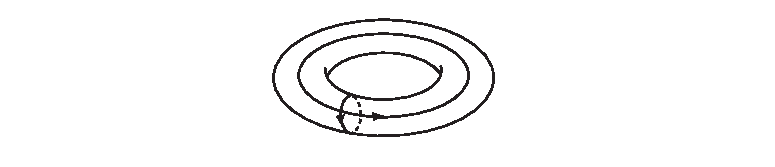
\includegraphics[width=.96\textwidth]{figures/7-8-1.pdf}\\图 7.8.1\end{center}
若两个类分别有阶 $k,\ell$，则除 $p+q$ 维张量项外，挠积还在 $p+q+1$ 维给出阶与 $n=\gcd(k,\ell)$ 有关的项。其几何来源较不直观。写 $kz=\partial d$、$\ell z'=\partial'd'$，则
\[
\overline\partial(d\otimes d')=n\left[\frac{k}{n}z\otimes d'+(-1)^{p+1}\frac{\ell}{n}d\otimes z'\right].
\]
方括号中的链是 $p+q+1$ 维闭链，其 $n$ 倍为边缘，展示了所需挠类的来源。

\subsection*{同调万有系数定理的证明}
取 $\mathcal C'$ 仅在零维为 $G$，其他维为零。此时 $\mathcal C\otimes\mathcal C'$ 就是 $\mathcal C\otimes G$，且第二因子的闭链显然为直和项。将 $H_0(\mathcal C')=G$、其余同调为零代入 Künneth 序列，立即得到定理 7.5.1 及分裂性。

\sourcepage{421}
\subsection*{域系数的 Künneth 定理}
若两链复形都是域 $F$ 上的向量空间且边缘线性，可使用 $\otimes_F$ 定义张量复形。

\entry{定理}{7.8.9（向量空间 Künneth 定理）}存在自然向量空间同构
\[
\bigoplus_{p+q=m}H_p(\mathcal E)\otimes_FH_q(\mathcal E')\cong H_m(\mathcal E\otimes_F\mathcal E').
\]
\textbf{证明：}重复前面证明的前四步，均保持有效。第五步中向量空间短正合列张量后仍短正合，不出现挠积项，所以连接同态的核为零，得到同构。\hfill$\square$

\sourcepage{422}
\entry{定理}{7.8.10（域系数 Künneth 定理）}对自由链复形，有自然同构
\[
\bigoplus_{p+q=m}H_p(\mathcal C;F)\otimes_FH_q(\mathcal C';F)
\cong H_m(\mathcal C\otimes\mathcal C';F).
\]
\translatornote{原书右侧把整数链复形之间的张量记为 $\otimes_F$，但它们未必为 $F$ 模；按证明，应先取整数张量积，再取 $F$ 系数同调。}

\textbf{证明：}对 $\mathcal E=\mathcal C\otimes F$、$\mathcal E'=\mathcal C'\otimes F$ 应用上一定理。只需识别
\[
(\mathcal C\otimes F)\otimes_F(\mathcal C'\otimes F)\cong(\mathcal C\otimes\mathcal C')\otimes F.
\]
定义 $(x\otimes\alpha)\otimes_F(y\otimes\beta)\mapsto(x\otimes y)\otimes\alpha\beta$。它先由四变量多线性映射诱导，再由标量平衡性下降为 $F$ 上张量积的映射。对自由基，它将 $(x_i\otimes1)\otimes_F(y_j\otimes1)$ 映到 $(x_i\otimes y_j)\otimes1$，所以为同构。它自然并保持边缘，故得同调同构。\hfill$\square$

\sourcepage{423}
\entry{例}{7.8.11}若 $K,L$ 中至少一个局部有限，则由乘积胞腔链复形及上述定理，
\[
\bigoplus_{p+q=m}H_p(K;F)\otimes_FH_q(L;F)\cong H_m(|K|\times|L|;F).
\]

\subsection*{习题}
\begin{enumerate}
\item 说明约化同调不能直接使用本节 Künneth 公式。
\item 对子复形 $K_0,L_0$，构造从相对链复形张量积到乘积空间偶的胞腔链复形的同调同构，空间偶为 $(|K|\times|L|,(|K_0|\times|L|)\cup(|K|\times|L_0|))$，推出相对单纯同调 Künneth 序列。
\item 若 $\mathcal C$ 自由，证明存在自然正合列，其左端为 $\bigoplus H_p(\mathcal C)\otimes H_q(\mathcal C';G)$，中间为 $H_m(\mathcal C\otimes\mathcal C';G)$，右端为 $\bigoplus H_{p-1}(\mathcal C)*H_q(\mathcal C';G)$。若第二复形自由，且 $G$ 无挠或其整数同调均无挠，证明序列分裂。
\item 补全推论 7.8.5 的证明。
\end{enumerate}

\section{Eilenberg--Zilber 定理}
\sourcepage{423--424}
本节证明，对任意拓扑空间 $X,Y$，$\mathcal S(X)\otimes\mathcal S(Y)$ 都能计算 $X\times Y$ 的奇异同调。证明的关键是无环模型定理。

\entry{引理}{7.9.1}若两个增广链复形无环，且第一因子自由，则其张量复形无环。

\textbf{证明：}由 Künneth 序列，两因子的同调仅在零维为 $\Z$，所有挠积项均为零，所以张量复形的同调只在零维为 $\Z\otimes\Z\cong\Z$，其余为零。这说明任意增广下其约化同调为零。\hfill$\square$

\entry{定理}{7.9.2（Eilenberg--Zilber 定理）}对每对拓扑空间，存在自然链映射
\[
\mu:\mathcal S(X)\otimes\mathcal S(Y)\to\mathcal S(X\times Y),\qquad
\nu:\mathcal S(X\times Y)\to\mathcal S(X)\otimes\mathcal S(Y),
\]
它们互为链同伦逆。

\textbf{证明：}在成对拓扑空间范畴上定义增广链复形函子 $G(X,Y)=\mathcal S(X)\otimes\mathcal S(Y)$、$G'(X,Y)=\mathcal S(X\times Y)$，态射分别为 $f_\#\otimes g_\#$、$(f\times g)_\#$。取模型族 $\{(\Delta_p,\Delta_q)\}$。

两函子在每个模型上无环：乘积单形可缩，另一个由上一引理。还需证明自由性，然后可直接应用无环模型定理，得到双向自然变换及复合到恒等的自然链同伦。

\sourcepage{425}
对 $G'$，每维 $m$ 只需模型 $(\Delta_m,\Delta_m)$ 及对角奇异单形 $d(x)=(x,x)$。其在 $(f,g)$ 下的像为 $x\mapsto(f(x),g(x))$，每个乘积空间奇异单形均唯一如此表示，故构成自由基。

对 $G$，$m$ 维模型取所有 $p+q=m$ 的 $(\Delta_p,\Delta_q)$，模型元素为 $i_p\otimes i_q$。它在 $(f,g)$ 下的像为 $f\otimes g$。因为每个奇异链群以所有奇异单形为自由基，定理 6.2.10 说明这些元素恰构成总张量链群的自由基。\hfill$\square$

\entry{定理}{7.9.3（拓扑空间的 Künneth 定理）}任意空间 $X,Y$ 有自然正合列
\[
\begin{split}
0\to\bigoplus_{p+q=m}H_p(X)\otimes H_q(Y)\to H_m(X\times Y)\\
\to\bigoplus_{p+q=m}H_{p-1}(X)*H_q(Y)\to0.
\end{split}
\]
它分裂，但分裂不自然。左侧映射为同调叉积，等于张量同态 $\Theta$ 后接 Eilenberg--Zilber 等价的 $\mu_*$。后面将更常用上同调中的类似叉积。

\sourcepage{426}
\entry{定理}{7.9.4}域 $F$ 系数下，有自然同构
\[
\bigoplus_{p+q=m}H_p(X;F)\otimes_FH_q(Y;F)\cong H_m(X\times Y;F).
\]
\translatornote{原书这里的张量积省略了下标 $F$；域系数版本应在 $F$ 上取张量积。}

为了以后应用，给出一个具体链等价公式。

\entry{定理}{7.9.5}令 $\pi_1,\pi_2$ 为乘积投影，定义
\[
\nu(T)=\sum_{i=0}^m[\pi_1\circ T\circ\ell(\epsilon_0,\ldots,\epsilon_i)]
\otimes[\pi_2\circ T\circ\ell(\epsilon_i,\ldots,\epsilon_m)].
\]
则 $\nu$ 是保持增广的自然链等价。

\textbf{证明：}自然性及保持增广留作习题。链映射性质需要繁琐但直接的计算。简记 $T_1[i_0,\ldots,i_k]=\pi_1T\ell(\epsilon_{i_0},\ldots,\epsilon_{i_k})$，$T_2$ 类似。展开后 $\overline\partial\nu(T)-\nu(\partial T)$ 等于
\[
\sum_{i=1}^{m}(-1)^iT_1[0,\ldots,i-1]\otimes T_2[i,\ldots,m]
+\sum_{i=0}^{m-1}(-1)^iT_1[0,\ldots,i]\otimes T_2[i+1,\ldots,m],
\]
两和逐项抵消。\translatornote{原书第二和的起点印为 $1$，遗漏 $i=0$ 项；否则不能与第一和完全抵消。}由 Eilenberg--Zilber 定理证明中的无环模型唯一性，这个自然、保持增广的链映射就是链等价。\hfill$\square$

\sourcepage{427}
原始证明不使用无环模型，而是给出 $\nu$ 及类似的 $\mu$ 的公式，再直接构造两个复合与恒等之间的链同伦。

\subsection*{习题}
\begin{enumerate}
\item 证明存在非自然同构 $H_m(X\times Y)\cong\bigoplus_{p+q=m}H_p(X;H_q(Y))$。
\item \begin{enumerate}[label=(\alph*)]
\item 对 $A\subset X,B\subset Y$，证明存在自然链等价，从 $\mathcal S(X,A)\otimes\mathcal S(Y,B)$ 到 $\mathcal S(X\times Y)/(\mathcal S(X\times B)+\mathcal S(A\times Y))$。
\item 若 $\{X\times B,A\times Y\}$ 可切除，陈述并证明相对奇异同调 Künneth 定理。
\end{enumerate}
\item 验证定理 7.9.5 的自然性、增广及链映射性质。
\item \begin{enumerate}[label=(\alph*)]
\item 对 CW 复形 $X,Y$，证明胞腔链复形的张量积可计算乘积空间同调。
\item 〔*〕证明它与 $\mathcal S(X)\otimes\mathcal S(Y)$ 实际上链等价。
\item 直接用 $\mathcal D(P^2)\otimes\mathcal D(P^3)$ 的群与边缘计算 $P^2\times P^3$ 的同调。
\item 用 Künneth 定理核对结果。
\end{enumerate}
\item 计算 $S^2\times P^5$、$P^3\times P^5$、$S^3\times L(n,k)$、$L(n,k)\times L(m,j)$、$S^1\times S^1\times S^3$、$\mathbb CP^2\times\mathbb CP^3$ 的同调。
\item 若紧连通 $n$ 维流形满足 $H_n(M)\cong\Z$，其 Betti 数、挠系数之间存在关系。利用上一题的结果提出猜想。
\item 验证定理 7.9.2 证明中两个函子的函子性质。
\end{enumerate}

\section{*上同调的 Künneth 定理}
\sourcepage{428--429}
要计算乘积空间的上同调，总可以先用 Künneth 定理计算其同调，再应用上同调的泛系数定理。不过，我们也希望有一个直接适用于上同调的 Künneth 定理。本节将证明这样的定理；下一节将用它计算乘积空间的上同调环。

先引入上同调的叉积运算。本节只给出定义，其性质留到下一节讨论。以下 $R$ 始终表示有单位元的交换环。

设 $C,C'$ 是链复形。与 $C$ 对应的上链复形 $\operatorname{Hom}(C,R)$ 在 $p$ 维的群为 $\operatorname{Hom}(C_p,R)$。同样有 $\operatorname{Hom}(C',R)$。按照预期的方式，使它们的张量积成为上链复形：其 $m$ 维群为
\[
\bigoplus_{p+q=m}\operatorname{Hom}(C_p,R)\otimes\operatorname{Hom}(C'_q,R),
\]
上边缘算子由下式给定：
\[
\delta(\varphi^p\otimes\psi^q)=\delta\varphi^p\otimes\psi^q+(-1)^p\varphi^p\otimes\delta'\psi^q.
\]
这里先应用 $\operatorname{Hom}$ 函子，再取张量积。也可以颠倒次序，得到上链复形 $\operatorname{Hom}(C\otimes C',R)$，其 $m$ 维群是 $\operatorname{Hom}((C\otimes C')_m,R)$。其上边缘算子是 $\partial$ 的对偶，记为 $\overline\partial$。这两个复形之间有如下自然同态。

\entry{定义}{7.10.1}设 $p+q=m$，定义
\[
\theta:\operatorname{Hom}(C_p,R)\otimes\operatorname{Hom}(C'_q,R)\longrightarrow\operatorname{Hom}((C\otimes C')_m,R)
\]
使得
\[
\langle\theta(\varphi^p\otimes\psi^q),c_r\otimes c'_s\rangle
=\langle\varphi^p,c_r\rangle\langle\psi^q,c'_s\rangle.
\]
约定当 $p\ne r$ 时 $\langle\varphi^p,c_r\rangle=0$，对 $\psi^q$ 也作同样约定。换言之，把 $\operatorname{Hom}(C_p,R)$ 的元素自动延拓为 $\bigoplus C_r$ 上的同态，在其他直和分量上取零，且不改变记号。

\entry{引理}{7.10.2}$\theta$ 是自然上链映射。

\textbf{证明：}设 $\varphi\in\operatorname{Hom}(C_p,R)$，$\psi\in\operatorname{Hom}(C'_q,R)$，$p+q=m$，并设 $r+s=m+1$。计算得
\begin{align*}
\langle\theta\delta(\varphi\otimes\psi),c_r\otimes c'_s\rangle
&=\langle\delta\varphi,c_r\rangle\langle\psi,c'_s\rangle
+(-1)^p\langle\varphi,c_r\rangle\langle\delta'\psi,c'_s\rangle,\\
\langle\overline\partial\theta(\varphi\otimes\psi),c_r\otimes c'_s\rangle
&=\langle\varphi,\partial c_r\rangle\langle\psi,c'_s\rangle
+(-1)^r\langle\varphi,c_r\rangle\langle\psi,\partial'c'_s\rangle.
\end{align*}
两式只有末项符号看似不同；若 $p=r$，符号相同；若 $p\ne r$，则 $\langle\varphi,c_r\rangle=0$，两个末项均为零。由定义还直接得到，对同态 $f:C_p\to D_p$、$g:C'_q\to D'_q$，
\[
\theta\circ(\overline f\otimes\overline g)=\overline{f\otimes g}\circ\theta.
\]
所以 $\theta$ 是自然的。\hfill$\square$

现在定义上同调中的同态，与同调 Künneth 定理中的 $\Theta$ 对应。

\entry{定义}{7.10.3}定义上同调的张量同态\translatornote{原文此处写作“同调的张量同态”，由定义的上下标及上下文可知指上同调。}
\[
\Theta:H^p(C;R)\otimes H^q(C';R)\longrightarrow H^m(C\otimes C';R),\qquad m=p+q,
\]
如下：若 $\varphi,\psi$ 分别是 $p,q$ 维上闭链，则令
\[
\Theta(\{\varphi\}\otimes\{\psi\})=\{\theta(\varphi\otimes\psi)\}.
\]
右端确为上闭链的类，因为
\[
\overline\partial\theta(\varphi\otimes\psi)
=\theta(\delta\varphi\otimes\psi+(-1)^p\varphi\otimes\delta'\psi)=0.
\]
类似计算说明改变上闭链代表元不改变所得上同调类，故 $\Theta$ 定义良好。

\sourcepage{430--431}
\entry{定义}{7.10.4}设 $X,Y$ 是拓扑空间，$m=p+q$。定义\emph{上同调叉积}为复合同态
\[
H^p(X;R)\otimes H^q(Y;R)\xrightarrow{\Theta}
H^m(\mathcal S(X)\otimes\mathcal S(Y);R)\xrightarrow{\nu^*}H^m(X\times Y;R),
\]
其中 $\nu$ 是定理 7.9.5 的 Eilenberg--Zilber 链等价。记此同态为 $\times$，并把 $\alpha^p\otimes\beta^q$ 的像记作 $\alpha^p\times\beta^q$。

与杯积一样，$\Theta$ 也可以对其他系数定义。下面给出一种推广。

\entry{定义}{7.10.5}设 $G$ 是阿贝尔群，$X,Y$ 是拓扑空间，$m=p+q$。定义叉积
\[
\times:H^p(X)\otimes H^q(Y;G)\longrightarrow H^m(X\times Y;G)
\]
为 $\nu^*\circ\Theta$；这里 $\Theta$ 由下列上链映射诱导：
\[
\langle\theta(\varphi^p\otimes\psi^q),c_r\otimes c'_s\rangle
=\langle\varphi^p,c_r\rangle\langle\psi^q,c'_s\rangle,
\quad \varphi^p\in\operatorname{Hom}(C_p,\Z),\quad
\psi^q\in\operatorname{Hom}(C'_q,G).
\]
右端乘法表示整数对 $G$ 的作用。

还应注意，$\operatorname{Hom}(C_p,R)$ 和 $\operatorname{Hom}(C'_q,R)$ 都是 $R$ 模，而且
\[
\theta(a\varphi\otimes\psi)=\theta(\varphi\otimes a\psi)=a\theta(\varphi\otimes\psi).
\]
因此 $\theta$ 诱导 $R$ 模同态
\[
\operatorname{Hom}(C_p,R)\otimes_R\operatorname{Hom}(C'_q,R)
\longrightarrow\operatorname{Hom}((C\otimes C')_m,R).
\]
特别地，当 $R$ 是域 $F$ 时，这是向量空间的线性映射。上述两种情形都诱导上同调上的同态 $\Theta$ 及叉积：前者为 $\Z,G$ 系数的叉积，后者为 $R$ 模同态
\[
H^p(X;R)\otimes_R H^q(Y;R)\xrightarrow{\times}H^m(X\times Y;R).
\]
最一般的叉积可相对于任意系数配对 $A\otimes_R A'\to A''$（一个 $R$ 模同态）来定义，本书不需要这样的普遍性。

\subsection*{整数系数上同调的 Künneth 定理}
证明的想法是把 $\operatorname{Hom}(C_p,\Z)$ 重新编号，使上链复形成为链复形，然后应用已经证明的 Künneth 定理。困难之一是这些群通常并不自由，因此需要某些限制条件。另一困难是，计算 $C\otimes C'$ 上同调所用的 $\operatorname{Hom}(C\otimes C',\Z)$，与要应用 Künneth 定理的 $\operatorname{Hom}(C,\Z)\otimes\operatorname{Hom}(C',\Z)$ 不同。映射 $\theta$ 正是在这里发挥作用。

\entry{引理}{7.10.6}设链复形 $C,C'$ 在某个维数以下为零。若 $C$ 自由且每维有限生成，则
\[
\theta:\bigoplus_{p+q=m}\operatorname{Hom}(C_p,\Z)\otimes\operatorname{Hom}(C'_q,\Z)
\longrightarrow\operatorname{Hom}((C\otimes C')_m,\Z)
\]
是同构。

\textbf{证明：}把 $\theta$ 分为两个映射的复合：先对各分量应用
\[
M:\operatorname{Hom}(C_p,\Z)\otimes\operatorname{Hom}(C'_q,\Z)
\to\operatorname{Hom}(C_p\otimes C'_q,\Z),
\]
其中 $M(\varphi\otimes\psi)(c\otimes c')=\varphi(c)\psi(c')$；再应用
\[
e:\bigoplus_{p+q=m}\operatorname{Hom}(C_p\otimes C'_q,\Z)
\to\operatorname{Hom}\left(\bigoplus_{p+q=m}C_p\otimes C'_q,\Z\right).
\]
对分量上的同态 $F$，$e(F)$ 在该分量上等于 $F$，在其他分量上为零。

第一步：$M$ 是同构。取 $C_p$ 的有限基 $a_1,\ldots,a_k$ 及对偶基 $\overline a_1,\ldots,\overline a_k$。$M$ 的定义域是 $k$ 个 $\operatorname{Hom}(C'_q,\Z)$ 的直和，第 $i$ 个分量为
$\langle\overline a_i\rangle\otimes\operatorname{Hom}(C'_q,\Z)$。
另一方面，$C_p\otimes C'_q$ 是 $k$ 个 $C'_q$ 的直和，第 $i$ 个分量为 $\langle a_i\rangle\otimes C'_q$。其对偶也就是 $k$ 个 $\operatorname{Hom}(C'_q,\Z)$ 的直和，第 $i$ 个分量由在所有 $j\ne i$ 的分量上为零的同态组成。$M$ 把定义域的第 $i$ 个分量同构地映到这个分量上，所以是同构。

第二步：$e$ 显然是单射。其像由那些只在有限多个直和分量上可能非零的同态组成。由于 $C,C'$ 在某维以下为零，固定 $m$ 后，$p+q=m$ 的非零分量只有有限多个，因此 $e$ 也是满射。\hfill$\square$

\sourcepage{432--433}
\entry{定理}{7.10.7（整数系数上同调的 Künneth 定理）}设 $C,C'$ 在某维以下为零。若 $C$ 自由且每维有限生成，则存在自然正合列
\[
\begin{split}
0\longrightarrow\bigoplus_{p+q=m}H^p(C)\otimes H^q(C')
\xrightarrow{\Theta}H^m(C\otimes C')\\
\longrightarrow\bigoplus_{p+q=m}H^{p+1}(C)*H^q(C')\longrightarrow0.
\end{split}
\]
若 $C'$ 也自由且每维有限生成，则此列分裂，但分裂不是自然的。

\textbf{证明：}定义链复形 $E,E'$，令
\[
E_{-p}=\operatorname{Hom}(C_p,\Z),\qquad E'_{-p}=\operatorname{Hom}(C'_p,\Z),
\]
边缘算子分别为 $\delta,\delta'$。$E$ 自由，因而 Künneth 定理给出正合列
\[
\begin{split}
0\to\bigoplus_{-p-q=-m}H_{-p}(E)\otimes H_{-q}(E')\to H_{-m}(E\otimes E')\\
\to\bigoplus_{-p-q=-m}H_{-p-1}(E)*H_{-q}(E')\to0.
\end{split}
\]
按定义 $H_{-p}(E)=H^p(C)$，$H_{-q}(E')=H^q(C')$。上一引理给出自然上链同构
\[
(E\otimes E')_{-m}=
\bigl(\operatorname{Hom}(C,\Z)\otimes\operatorname{Hom}(C',\Z)\bigr)^m
\xrightarrow{\theta}\operatorname{Hom}((C\otimes C')_m,\Z),
\]
从而诱导 $H_{-m}(E\otimes E')\cong H^m(C\otimes C')$。合并这些事实便得到所需正合列。其左端映射是包含映射与 $\theta$ 所诱导映射的复合，所以恰为 $\Theta$。若 $C'$ 也自由且每维有限生成，则 $E'$ 自由，正合列分裂。\hfill$\square$

\entry{推论}{7.10.8}上一定理中“$C$ 每维有限生成”的条件可以换成“每个 $H_i(C)$ 有限生成”。同样，“$C'$ 每维有限生成”的条件可以换成“每个 $H_i(C')$ 有限生成”。

\textbf{证明：}类似于定理 7.6.2。若 $C$ 自由、在某维以下为零，且每个 $H_i(C)$ 有限生成，则由引理 7.6.3，可以选取自由链复形 $D$，它在某维以下为零、每维有限生成，且 $H_i(D)\cong H_i(C)$。由定理 5.6.2，存在在所有维数诱导同调同构的链映射 $\varphi:C\to D$；由定理 5.7.2，它是链等价。因此
\[
\varphi\otimes i':C\otimes C'\to D\otimes C'
\]
也是链等价（见第 7.7 节习题）。Künneth 定理适用于 $D\otimes C'$，所以也适用于 $C\otimes C'$。正合列的自然性与定理 7.6.2 的证明相同。若每个 $H_i(C')$ 有限生成，也同样以每维有限生成且链等价的 $D'$ 代替 $C'$。\hfill$\square$

由此又得到拓扑空间的 Künneth 定理。

\entry{定理}{7.10.9（拓扑空间上同调的 Künneth 定理）}设 $X,Y$ 是拓扑空间。若每个 $H_i(X)$ 有限生成，则存在自然正合列
\[
\begin{split}
0\to\bigoplus_{p+q=m}H^p(X)\otimes H^q(Y)\xrightarrow{\times}H^m(X\times Y)\\
\to\bigoplus_{p+q=m}H^{p+1}(X)*H^q(Y)\to0.
\end{split}
\]
若每个 $H_i(Y)$ 也有限生成，则此列分裂，但分裂不是自然的。

\sourcepage{434--435}
\subsection*{域系数上同调的 Künneth 定理}
与同调的情形一样，系数取在域中时，Künneth 定理大为简化。

\entry{定理}{7.10.10（域系数上同调的 Künneth 定理）}设 $F$ 是域，$C,C'$ 是在某维以下为零的链复形。若 $C$ 自由，且每个 $H_i(C)$ 有限生成，则存在自然同构
\[
\Theta:\bigoplus_{p+q=m}H^p(C;F)\otimes_F H^q(C';F)
\longrightarrow H^m(C\otimes C';F).
\]

\textbf{证明：}按通常的论证，可以假设 $C$ 本身每维有限生成。令
\[
E_{-p}=\operatorname{Hom}(C_p,F),\qquad E'_{-q}=\operatorname{Hom}(C'_q,F).
\]
这是 $F$ 上的向量空间链复形。向量空间的 Künneth 定理（定理 7.8.9）给出自然线性同构
\[
\bigoplus_{p+q=m}H_{-p}(E)\otimes_F H_{-q}(E')\longrightarrow H_{-m}(E\otimes_F E').
\]
由于 $C,C'$ 在某维以下为零，且 $C$ 自由、每维有限生成，引理 7.10.6 的证明几乎原样适用，表明 $\theta$ 给出 $E\otimes_F E'$ 与 $\operatorname{Hom}(C\otimes C',F)$ 之间的线性同构，而且是上链映射。结论随即成立。\hfill$\square$

\entry{推论}{7.10.11}设 $F$ 是域，$X,Y$ 是拓扑空间。若每个 $H_i(X)$ 有限生成，则存在自然线性同构
\[
\bigoplus_{p+q=m}H^p(X;F)\otimes_F H^q(Y;F)\xrightarrow{\times}H^m(X\times Y;F).
\]

\subsection*{习题}
\begin{enumerate}
\item 陈述并证明相对奇异上同调的 Künneth 定理。〔参见第 7.9 节习题 2。〕
\item 计算下列空间的上同调群。可以使用 Künneth 定理，也可以对第 7.9 节习题 5 的结果应用泛系数定理。
\begin{enumerate}[label=(\alph*)]
\item $S^2\times P^5$；\item $P^3\times P^5$；\item $S^3\times L(n,k)$；
\item $L(n,k)\times L(m,j)$；\item $S^1\times S^1\times S^3$；\item $\mathbb{CP}^2\times\mathbb{CP}^3$。
\end{enumerate}
\item 设 $M$ 是紧致连通 $n$ 维流形，且 $H_n(M)\cong\Z$。$M$ 的同调群与上同调群之间存在某些关系。把上一题的计算与第 7.9 节习题 5 中的计算比较，提出关于这些关系的猜想。
\item 计算以下空间的上同调群：
\begin{enumerate}[label=(\alph*)]
\item $S^1\times P^3$；\item $P^2\times P^4$；\item $S^2\times L(n,k)$。
\end{enumerate}
\end{enumerate}

\section{*应用：乘积空间的上同调环}
\sourcepage{435--436}
上一节定义了上同调叉积，并用它得到上同调的 Künneth 定理。本节考察叉积的一些性质，并用来研究上同调的环结构。先对环 $R$ 系数的叉积（定义 7.10.4）陈述结论，再说明这些结论在多大程度上也适用于 $\Z,G$ 系数的叉积（定义 7.10.5）。设 $X,Y$ 是拓扑空间。

\entry{定义}{7.11.1}叉积是上同调同态 $\Theta$ 与 $\nu^*$ 的复合。这两个同态分别由上链映射 $\theta$ 和 $\overline\nu$ 诱导，因此叉积由 $\overline\nu\circ\theta$ 诱导。相应地定义
\[
c^p\times c^q=\overline\nu\theta(c^p\otimes c^q),
\]
称为\emph{上链叉积}。它诱导上同调叉积。

若 $m=p+q$，$T:\Delta_m\to X\times Y$，则
\begin{align*}
\langle c^p\times c^q,T\rangle
&=\langle\theta(c^p\otimes c^q),\nu(T)\rangle\\
&=\sum_{i=0}^m\langle c^p,\pi_1T\ell(\epsilon_0,\ldots,\epsilon_i)\rangle
\langle c^q,\pi_2T\ell(\epsilon_i,\ldots,\epsilon_m)\rangle.
\end{align*}
和式中只有 $i=p$ 的项可能非零。因此得到：

\entry{引理}{7.11.2}上链叉积由下式给出：
\[
\langle c^p\times c^q,T\rangle=
\langle c^p,\pi_1T\ell(\epsilon_0,\ldots,\epsilon_p)\rangle
\langle c^q,\pi_2T\ell(\epsilon_p,\ldots,\epsilon_m)\rangle.
\]
这个结论也适用于 $\Z,G$ 系数。它表示，$c^p\times c^q$ 在 $T$ 上的值，等于 $c^p$ 在 $T$ 第一分量的前面上的值，乘以 $c^q$ 在第二分量的后面上的值。

\entry{定理}{7.11.3}叉积具有以下性质。
\begin{enumerate}[label=(\alph*)]
\item 若 $\lambda:X\times Y\to Y\times X$ 交换坐标，则
\[\lambda^*(\beta^q\times\alpha^p)=(-1)^{pq}\alpha^p\times\beta^q.\]
\item 在 $H^*(X\times Y\times Z;R)$ 中，
\[(\alpha\times\beta)\times\gamma=\alpha\times(\beta\times\gamma).\]
\item 设 $\pi_1,\pi_2$ 是两个投影，$1_X,1_Y$ 是相应上同调环的单位元，则
\[\pi_1^*(\alpha^p)=\alpha^p\times1_Y,\qquad \pi_2^*(\beta^q)=1_X\times\beta^q.\]
\end{enumerate}

\textbf{证明：}(a) 定义
\[
\omega:(\mathcal S(X)\otimes\mathcal S(Y))_m\to(\mathcal S(Y)\otimes\mathcal S(X))_m,
\quad\omega(c_p\otimes c_q)=(-1)^{pq}c_q\otimes c_p.
\]
可检验 $\omega$ 是链映射；若没有符号 $(-1)^{pq}$，就不再是链映射。我们要证明
\[
\omega\nu\simeq\nu\lambda_\#.
\]
\sourcepage{437}
已知 $\lambda_\#$ 和 $\nu$ 保持增广，且对于连续映射诱导的同态是自然的；$\omega$ 也有这些性质。考虑函子
\[
\begin{array}{ll}
G(X,Y)=\mathcal S(X\times Y),&G(f,g)=(f\times g)_\#,\\
G'(X,Y)=\mathcal S(Y)\otimes\mathcal S(X),&G'(f,g)=g_\#\otimes f_\#.
\end{array}
\]
已经证明它们相对于模型族 $\{(\Delta_p,\Delta_q)\}$ 自由且无环。因此 $G$ 到 $G'$ 的任意两个保持增广的自然变换自然链同伦。$\omega\nu$ 和 $\nu\lambda_\#$ 正是这样的自然变换，所以链同伦。

对偶化上述关系，并定义
\[
\eta(c^q\otimes c^p)=(-1)^{pq}c^p\otimes c^q.
\]
直接检验得到
\[\theta\eta=\overline\omega\theta.\]
另一方面，由刚证明的链同伦得到
\[\overline\nu\,\overline\omega\simeq\lambda^\#\overline\nu.\]
因此，由 $\eta,\theta,\overline\nu,\lambda^\#$ 组成的对偶图在上同调上交换，从而得到 (a)。

(b)、(c) 也可以用无环模型论证，但用引理 7.11.2 的上链公式更容易。将该公式应用两次，立即得到 (b)。

为验证 (c)，取代表 $\alpha^p$ 的上闭链 $z^p$，并令 $z^0$ 为 $Y$ 上在每个奇异零单形上取值 $1$ 的上闭链。$\alpha^p\times1_Y$ 由 $z^p\times z^0$ 代表。对 $T:\Delta_p\to X\times Y$，有
\begin{align*}
\langle z^p\times z^0,T\rangle
&=\langle z^p,\pi_1T\ell(\epsilon_0,\ldots,\epsilon_p)\rangle
\langle z^0,\pi_2T\ell(\epsilon_p)\rangle\\
&=\langle z^p,\pi_1T\rangle=\langle\pi_1^\#z^p,T\rangle.
\end{align*}
所以 $\alpha^p\times1_Y=\pi_1^*(\alpha^p)$。另一个等式同理。\hfill$\square$

经过适当解释，三种性质也都适用于另一种系数的叉积。(a) 中右端取 $\Z,G$ 系数，左端相应交换系数次序；(b) 在三个系数群中两个为 $\Z$、一个为 $G$ 时成立；(c) 的第一个等式在 $1_Y\in H^0(Y)$、$\alpha^p\in H^p(X;G)$ 时成立，因为此时 $\alpha^p\times1_Y\in H^p(X\times Y;G)$，等式有意义。另一个等式也作同样解释。

\sourcepage{438}
上链叉积公式与杯积公式十分相似，这提示二者之间存在关系。下一定理给出这种关系。

\entry{定理}{7.11.4}设 $d:X\to X\times X$ 为对角映射 $d(x)=(x,x)$，则对两种系数的叉积都有
\[d^*(\alpha^p\times\beta^q)=\alpha^p\smile\beta^q.\]

\textbf{证明：}取代表上闭链 $z^p,z^q$。对奇异单形 $T:\Delta_{p+q}\to X$，令 $m=p+q$，则
\begin{align*}
\langle d^\#(z^p\times z^q),T\rangle
&=\langle z^p\times z^q,dT\rangle\\
&=\langle z^p,\pi_1dT\ell(\epsilon_0,\ldots,\epsilon_p)\rangle
\langle z^q,\pi_2dT\ell(\epsilon_p,\ldots,\epsilon_m)\rangle\\
&=\langle z^p\smile z^q,T\rangle,
\end{align*}
这里使用了 $\pi_1d=i_X=\pi_2d$。\hfill$\square$

这一定理归功于 Lefschetz。它说明为何上同调具有环结构，而同调没有相应的这种结构。同调和上同调都有叉积，但只有在上同调中，才能把叉积与对角映射诱导的同态复合。在同调中，相应的图为
\[
H_p(X)\otimes H_q(X)\xrightarrow{\times}H_{p+q}(X\times X)
\xleftarrow{d_*}H_{p+q}(X),
\]
其中 $d_*$ 的方向不允许作所需的复合！

\entry{推论}{7.11.5}两种系数的杯积均满足反交换律
\[\alpha^p\smile\beta^q=(-1)^{pq}\beta^q\smile\alpha^p.\]

\textbf{证明：}设 $\lambda:X\times X\to X\times X$ 交换坐标。由于 $\lambda d=d$，
\begin{align*}
\alpha^p\smile\beta^q
&=d^*(\alpha^p\times\beta^q)
=d^*\lambda^*(\alpha^p\times\beta^q)\\
&=(-1)^{pq}d^*(\beta^q\times\alpha^p)
=(-1)^{pq}\beta^q\smile\alpha^p.
\end{align*}
\translatornote{原文此处有将 $pq$ 印作 $pg$、并在中间一步把叉积写作杯积的排印错误；这里按定义写出。}\hfill$\square$

下面计算乘积空间上同调中的杯积。

\entry{定理}{7.11.6}在 $H^*(X\times Y;R)$ 中，
\[
(\alpha\times\beta)\smile(\alpha'\times\beta')
=(-1)^{pq}(\alpha\smile\alpha')\times(\beta\smile\beta'),
\qquad p=\dim\alpha',\quad q=\dim\beta.
\]

\sourcepage{439}
\textbf{证明：}设 $\pi_1,\pi_2$ 为投影。

第一步：先证明 $\beta$ 和 $\alpha'$ 都为各自环的单位元时的公式。设 $z^p,z^q$ 分别代表 $\alpha,\beta'$。由上链叉积公式，
\begin{align*}
\langle z^p\times z^q,T\rangle
&=\langle z^p,\pi_1T\ell(\epsilon_0,\ldots,\epsilon_p)\rangle
\langle z^q,\pi_2T\ell(\epsilon_p,\ldots,\epsilon_m)\rangle\\
&=\langle\pi_1^\#z^p,T\ell(\epsilon_0,\ldots,\epsilon_p)\rangle
\langle\pi_2^\#z^q,T\ell(\epsilon_p,\ldots,\epsilon_m)\rangle\\
&=\langle\pi_1^\#z^p\smile\pi_2^\#z^q,T\rangle.
\end{align*}
因此
\[\alpha\times\beta'=\pi_1^*(\alpha)\smile\pi_2^*(\beta')
=(\alpha\times1_Y)\smile(1_X\times\beta').\]

第二步：证明 $\beta,\beta'$ 都为单位元时的公式。杯积的自然性给出
\[\pi_1^*(\alpha)\smile\pi_1^*(\alpha')=\pi_1^*(\alpha\smile\alpha'),\]
也就是
\[(\alpha\times1_Y)\smile(\alpha'\times1_Y)=(\alpha\smile\alpha')\times1_Y.\]
对第二因子也有同样结论。

第三步：一般情形由前两步及反交换律得到：
\begin{align*}
(\alpha\times\beta)\smile(\alpha'\times\beta')
&=(\alpha\times1_Y)\smile(1_X\times\beta)\smile(\alpha'\times1_Y)\smile(1_X\times\beta')\\
&=(-1)^{pq}(\alpha\times1_Y)\smile(\alpha'\times1_Y)\smile(1_X\times\beta)\smile(1_X\times\beta')\\
&=(-1)^{pq}(\alpha\smile\alpha')\times(\beta\smile\beta').
\end{align*}
\hfill$\square$

这一定理使我们能够由两个因子的杯积，计算乘积空间上同调环中某些元素的杯积。当上同调 Künneth 定理适用时，可以更正式地表述为定理 7.11.8。

\entry{定义}{7.11.7}在 $H^*(X;R)\otimes_R H^*(Y;R)$ 上定义环结构：对 $\beta\in H^p(Y;R)$、$\alpha'\in H^q(X;R)$，令
\[
(\alpha\otimes\beta)\smile(\alpha'\otimes\beta')
=(-1)^{pq}(\alpha\smile\alpha')\otimes(\beta\smile\beta').
\]
读者可检验此运算定义良好，且满足环公理；特别是其中的符号使结合律成立。

\sourcepage{440--441}
\entry{定理}{7.11.8}若所有 $H_i(X)$ 都有限生成，则叉积给出环单同态
\[\times:H^*(X)\otimes H^*(Y)\longrightarrow H^*(X\times Y).\]
若 $F$ 是域，则
\[\times:H^*(X;F)\otimes_F H^*(Y;F)\longrightarrow H^*(X\times Y;F)\]
是代数同构。

\entry{例}{7.11.9}考虑 $S^n\times S^m$ 的上同调环，其中 $n,m\ge1$。取生成元 $\alpha^n\in H^n(S^n)$、$\beta^m\in H^m(S^m)$。则 $H^*(S^n\times S^m)$ 是秩为 $4$ 的自由群，基为
\[1\times1,\quad\alpha\times1,\quad1\times\beta,\quad\alpha\times\beta.\]
正维元素之间唯一的非平凡乘积（以及由反交换律得到的乘积）是
\[(\alpha\times1)\smile(1\times\beta)=\alpha\times\beta.\]

特别地，$n=m=1$ 时空间是环面，这就是例 5.10.5 中已计算的上同调环。下面把这些类画出来。用图 7.11.1 中的通常方式表示环面。设 $X$ 是子空间 $abca$，则其一维上同调生成元 $\alpha$ 由上闭链 $x^1=[b,c]^*$ 代表。投影 $\pi_1$ 是单纯映射，因此 $\pi_1^\#(x^1)$ 就是图中的环面上闭链 $w^1$，代表 $\alpha\times1$。类似地，图 7.11.2 的上闭链 $z^1$ 代表 $1\times\beta$，其中 $\beta$ 由空间 $Y=adea$ 上的 $[d,e]^*$ 代表。杯积 $(\alpha\times1)\smile(1\times\beta)=\alpha\times\beta$ 生成 $H^2(T)$。

\begin{figure}[htbp]\centering
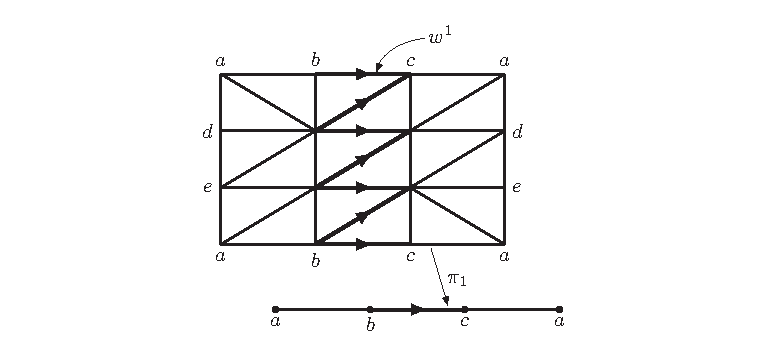
\includegraphics[width=.86\textwidth]{figures/7-11-1.pdf}
\caption*{图 7.11.1}
\end{figure}
\begin{figure}[htbp]\centering
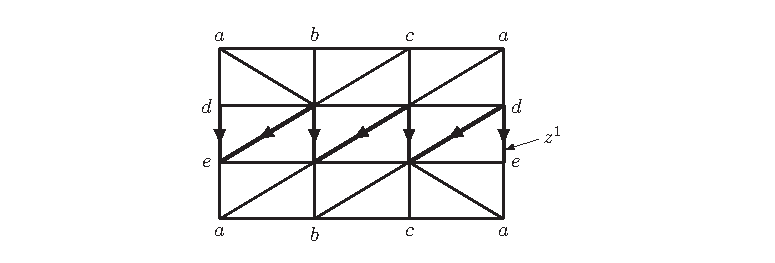
\includegraphics[width=.86\textwidth]{figures/7-11-2.pdf}
\caption*{图 7.11.2}
\end{figure}

\entry{例}{7.11.10}考虑 $P^2\times P^2$ 的 $\Z/2$ 系数上同调环。设 $\alpha\in H^1(P^2;\Z/2)$ 是非零元，则 $\alpha^2=\alpha\smile\alpha\ne0$（见第 5.10 节习题）。由定理 7.11.8，$H^*(P^2\times P^2;\Z/2)$ 是九维向量空间，各维的基如下：
\[
\begin{array}{c|l}
0&1\times1\\
1&\alpha\times1,\quad1\times\alpha\\
2&\alpha^2\times1,\quad\alpha\times\alpha,\quad1\times\alpha^2\\
3&\alpha^2\times\alpha,\quad\alpha\times\alpha^2\\
4&\alpha^2\times\alpha^2
\end{array}
\]
其乘法表容易写出。系数域为 $\Z/2$，所以不涉及符号问题。

下面的定义将在习题 3 中使用。

\entry{定义}{7.11.11}若 $M,N$ 是连通 $n$ 维流形，分别从中去掉一个开 $n$ 维球，再沿边界把剩余部分粘合，所得空间称为\emph{连通和}（connected sum），记为 $M\mathbin{\#}N$。对习题 3 中的流形，所得流形在同胚意义下定义良好；一般情形还必须考虑“定向”问题。

\sourcepage{441--442}
\subsection*{习题}
\begin{enumerate}
\item \begin{enumerate}[label=(\alph*)]
\item 设 $A\subset X$、$B\subset Y$。证明：若 $\{X\times B,A\times Y\}$ 是切除偶，则对通常采用的系数，存在相对上同调叉积
\[H^p(X,A)\otimes H^q(Y,B)\xrightarrow{\times}
H^{p+q}(X\times Y,(X\times B)\cup(A\times Y)).\]
\item 对相对杯积证明定理 7.11.4 和推论 7.11.5。
\end{enumerate}
\item \begin{enumerate}[label=(\alph*)]
\item 按本节方式定义叉积，并用 $\alpha\smile\beta=d^*(\alpha\times\beta)$ 定义杯积，其中 $d$ 是对角映射。利用叉积性质证明杯积双线性、满足结合律，且 $\{z^0\}$ 起单位元作用。
\item 按第 5.9 节定义杯积，再用 $\alpha\times\beta=\pi_1^*(\alpha)\smile\pi_2^*(\beta)$ 定义叉积，其中 $\pi_1,\pi_2$ 是投影。利用杯积性质证明叉积双线性、满足结合律，并证明
\[\pi_1^*(\alpha)=\alpha\times1_Y,\qquad\alpha\smile\beta=d^*(\alpha\times\beta).\]
\end{enumerate}
\item 计算下列上同调环：
\begin{enumerate}[label=(\alph*)]
\item $H^*(S^1\times S^1\times S^3)$。
\item $H^*((T\mathbin{\#}T)\times S^3)$，其中 $T$ 是环面。
\item $H^*((S^1\times S^5)\mathbin{\#}(S^2\times S^4))$。
\end{enumerate}
\item 设 $M$ 为紧致连通 $n$ 维流形，$H_n(M)\cong\Z$。利用上一题结果，对杯积
\[H^k(M)\otimes H^{n-k}(M)\longrightarrow H^n(M)\]
提出一个猜想。
\item 设 $S$ 为 Klein 瓶，$T$ 为环面。计算：
\begin{enumerate}[label=(\alph*)]
\item $H^*(T\times S)$；\item $H^*(T\times S;\Z/2)$。
\end{enumerate}
\item 验证定理 7.11.3(a) 证明中的 $\omega$ 是链映射。
\end{enumerate}

\chapter{流形中的对偶性}
\section{引言}
\sourcepage{443}
如前所述，流形是数学中最熟悉、最重要的一类几何对象。数学家经过相当长的时间，才给出流形概念的严格定义。最终，Hermann Weyl 在其关于 Riemann 曲面的著作中明确了这一概念。\footnote{\textit{Die Idee der Riemannschen Fläche}，Teubner，Leipzig--Berlin，1913。第三版的英译本见参考文献 [Wey64]。}

关于流形所证明的定理，往往不仅对拓扑学有用，而且对微分几何及其他数学分支也有用。对偶定理正是这样的例子。

对于任意拓扑空间，同调群与上同调群之间已有一种关系，即上同调的泛系数定理所表达的关系。对流形而言，还存在第二种关系，这就是著名的 Poincaré 对偶定理。如果把泛系数定理看作表达上同调与同调之间的一种代数对偶性，那么 Poincaré 对偶性从根本上说可以看作一种几何性质。这种对偶性并不对任意空间成立，而是特别依赖于流形所具有的性质。

这两类几何与代数的对偶性之间存在相互作用。这种相互作用有一些有趣的应用；我们将把它用于计算流形的上同调环。

还有其他对偶定理，分别以 Lefschetz、Alexander 和 Pontryagin 的名字命名。我们将在适当时候研究它们。这些定理都涉及流形的代数拓扑性质。

在以下讨论中，假定读者熟悉局部同调群（第 4.8 节）。

\section{两个复形的联结}
\sourcepage{444--445}
本节引入两个复形的联结，并考察它的一些性质。

\entry{定义}{8.2.1}设 $K,L$ 是欧氏空间 $E^J$ 中的非空复形，其一般单形分别写作 $s=v_0\cdots v_m$ 和 $t=w_0\cdots w_n$。假定对任意 $s\in K,t\in L$，点
\[v_0,\ldots,v_m,w_0,\ldots,w_n\]
都仿射无关，记它们张成的单形为
\[s*t=v_0\cdots v_mw_0\cdots w_n.\]
如果所有这样的单形及其面构成单纯复形，就称此复形为 $K$ 与 $L$ 的\emph{联结}（join），记为 $K*L$。

若 $K$ 只有一个顶点 $v$，则 $v*L$ 就是已经定义的 $L$ 上的锥。若 $K$ 由两个点组成，则 $K*L$ 称为 $L$ 的\emph{悬挂}，记为 $S(L)$。下一引理给出一般情形下联结存在的条件。

\entry{引理}{8.2.2}设 $K,L$ 是 $E^J$ 中不交的非空复形。
\begin{enumerate}[label=(\alph*)]
\item 若 $K*L$ 存在，则其多面体等于连接 $|K|$ 中点与 $|L|$ 中点的所有线段的并。任意两条不同的这样的线段至多在一个公共端点相交。
\item 反之，若连接两空间中点的任意两条不同线段至多在一个公共端点相交，则 $K*L$ 存在。
\end{enumerate}

\textbf{证明：}第一步：先证明单形情形。设 $\sigma=v_0\cdots v_mw_0\cdots w_n$，$s=v_0\cdots v_m$，$t=w_0\cdots w_n$。则 $\sigma$ 等于连接 $s$ 中点与 $t$ 中点的所有线段的并，不同的这样的线段至多在公共端点相交；此外，$\Int\sigma$ 等于连接 $\Int s$ 中点与 $\Int t$ 中点的所有开线段的并。这是第 1.2 节的一道习题，现在给出证明。

先证关于内部的断言。若 $p=\lambda x+(1-\lambda)y$，其中 $0<\lambda<1$，$x\in\Int s,y\in\Int t$，写
\[x=\sum\alpha_i v_i,\qquad y=\sum\beta_jw_j,\qquad
\alpha_i,\beta_j>0,\quad\sum\alpha_i=\sum\beta_j=1.\]
则 $p=\sum(\lambda\alpha_i)v_i+\sum(1-\lambda)\beta_jw_j$ 的系数都正且总和为 $1$，故 $p\in\Int\sigma$。反之，若
\[p=\sum\gamma_iv_i+\sum\delta_jw_j\in\Int\sigma,\]
其中所有系数均正、总和为 $1$，令 $\lambda=\sum\gamma_i$，$\alpha_i=\gamma_i/\lambda$，$\beta_j=\delta_j/(1-\lambda)$，则
\[p=\lambda\sum\alpha_iv_i+(1-\lambda)\sum\beta_jw_j,\]
所以 $p$ 位于连接两内部点的开线段上。

再证关于整个单形的断言。$\sigma$ 凸，所以包含所有连接 $s,t$ 中点的线段。反之，若 $x\in\sigma$ 且 $x$ 既不在 $s$ 中也不在 $t$ 中，则 $x$ 位于某个面 $\sigma'$ 的内部，且 $\sigma'$ 与 $s,t$ 都有公共顶点。由刚证明的结论，$x$ 位于连接 $\sigma'\cap s$ 中点与 $\sigma'\cap t$ 中点的开线段上。

最后证明交点性质。若同一点 $p$ 有两种表达
\[
p=\lambda\sum\alpha_iv_i+(1-\lambda)\sum\beta_jw_j
=\lambda'\sum\alpha'_iv_i+(1-\lambda')\sum\beta'_jw_j,
\]
其中 $0\le\lambda,\lambda'\le1$，各重心系数非负，各组和为 $1$，则由顶点仿射无关得到
\[\lambda\alpha_i=\lambda'\alpha'_i,\qquad
(1-\lambda)\beta_j=(1-\lambda')\beta'_j.\]
第一组求和得 $\lambda=\lambda'$。若它等于 $0$ 或 $1$，则 $p$ 是两线段的公共端点；否则各重心系数相等，两线段实际相同。

第二步：证明 (a)。考虑不同线段 $xy,x'y'$，其中
\[x\in\Int s,\quad x'\in\Int s',\quad y\in\Int t,\quad y'\in\Int t',
\qquad s,s'\in K,\quad t,t'\in L.\]
由第一步，
\[xy\subset\Int s\cup\Int(s*t)\cup\Int t,\qquad
x'y'\subset\Int s'\cup\Int(s'*t')\cup\Int t'.\]
\sourcepage{446}
因为 $K*L$ 是复形，若 $s\ne s'$ 且 $t\ne t'$，这些开单形两两不交，故两线段不交。若 $s=s'$ 而 $t\ne t'$，交点只能在 $\Int s$ 中，因此至多是两线段的公共端点。$s\ne s',t=t'$ 的情形同理；若 $s=s',t=t'$，则由第一步得到结论。

第三步：证明 (b)。先证明任意 $s=v_0\cdots v_m\in K$、$t=w_0\cdots w_n\in L$ 的全部顶点仿射无关。考虑线性奇异单形
\[\ell=\ell(v_0,\ldots,v_m,w_0,\ldots,w_n):\Delta_{m+n+1}\to E^J.\]
它把连接 $\epsilon_0\cdots\epsilon_m$ 中点与 $\epsilon_{m+1}\cdots\epsilon_{m+n+1}$ 中点的线段，线性映到连接 $s,t$ 中点的线段。由假设及第一步，$\ell$ 是单射。因此这些顶点张成的仿射平面维数必须是 $m+n+1$，否则 $\ell$ 不可能为单射。所以顶点仿射无关。

还需证明所得单形组成复形。如果两个不同的单形内部相交，除去 $K,L$ 本身已为复形的情形，其中一个必为 $s*t$。$\Int(s*t)$ 中每点都位于连接 $|K|$ 与 $|L|$ 中点的开线段上。如果它与 $\Int(s'*t')$ 相交，就有两条不同开线段相交；如果它与 $\Int s'$ 或 $\Int t'$ 相交，则某条这样的线段的内点同时是另一条的端点。这些都违反假设。因此所得单形确实组成复形。\hfill$\square$

若给定复形 $K,L$ 的欧氏空间位置使联结无法定义，可以找出分别与它们同构的复形 $K_0,L_0$，使 $K_0*L_0$ 存在。例如，可把它们取为某个标准单形 $\Delta^J$ 的两个不交子复形。

\entry{引理}{8.2.3}假设 $K*L$ 存在且 $K$ 局部有限。则
\[
\pi:|K|\times|L|\times I\to|K*L|,\qquad
\pi(x,y,t)=(1-t)x+ty
\]
是商映射。它把每个 $x\times|L|\times0$ 压成一点，把每个 $|K|\times y\times1$ 压成一点，除此之外是一一的。

\textbf{证明：}先用第 2.8 节的结果，证明定义域拓扑由各 $\sigma\times\tau\times I$（$\sigma\in K,\tau\in L$）协调。$|L|\times I$ 的拓扑由各 $\tau\times I$ 协调；$|K|$ 是局部紧 Hausdorff 空间，因此乘积拓扑由各 $|K|\times\tau\times I$ 协调。又因 $\tau\times I$ 局部紧 Hausdorff（事实上紧致），后者的拓扑由各 $\sigma\times\tau\times I$ 协调。故一个集合在整个乘积中闭，当且仅当它与每个这样子空间的交在该子空间中闭。

\sourcepage{447}
按定义，$\pi:\sigma\times\tau\times I\to\sigma*\tau$ 连续，因为二者都有欧氏子空间拓扑。$\sigma*\tau$ 到 $|K*L|$ 的包含也连续，因此 $\pi$ 的各个限制连续。由协调拓扑性质，$\pi$ 连续。

若 $\pi^{-1}(A)$ 闭，则它与每个 $\sigma\times\tau\times I$ 的交闭，因而紧致。其像 $A\cap(\sigma*\tau)$ 紧致，因而闭。于是 $A$ 在 $|K*L|$ 中闭，证明 $\pi$ 是商映射。它恰好实施所述粘合，则由引理 8.2.2 得到。\hfill$\square$

\entry{记号}{8.2.4}用 $X\approx Y$ 表示拓扑空间 $X,Y$ 同胚。

\entry{推论}{8.2.5}设 $K*L$ 与 $M*N$ 均有定义，且 $K$ 局部有限。如果 $|K|\approx|M|$、$|L|\approx|N|$，则 $|K*L|\approx|M*N|$。

\textbf{证明：}$|K|$ 局部紧，故 $|M|$ 也局部紧，从而 $M$ 局部有限。若 $h:|K|\to|M|$、$k:|L|\to|N|$ 为同胚，则 $h\times k\times i_I$ 通过上一引理的商映射诱导联结之间的同胚；它在 $|K|,|L|$ 上分别等于 $h,k$。\hfill$\square$

\entry{引理}{8.2.6}设 $J,K,L$ 是复形，且 $J*K$、$(J*K)*L$ 存在。则
\[J*K=K*J,\qquad (J*K)*L=J*(K*L).\]

\textbf{证明：}定义的对称性给出第一个等式。若第二式左端存在，则对 $J,K,L$ 的任意单形，其全部顶点仿射无关，且它们张成的单形及其面组成复形。这恰好也是右端复形的描述。\hfill$\square$

\entry{定理}{8.2.7}假设 $K*L$ 存在。若 $|L|\approx S^{n-1}$，则对所有 $i$，
\[\widetilde H_{i+n}(K*L)\cong\widetilde H_i(K).\]

\textbf{证明：}$n=1$ 时，$|L|$ 由两个点组成，$K*L$ 就是 $K$ 的悬挂，所需同构由 Mayer--Vietoris 序列得到（定理 3.4.6）。

一般情形用归纳法。设结论对 $n$ 成立，证明对 $n+1$ 成立。由推论 8.2.5，只需选取一个空间同胚于 $S^n$ 的特定复形 $L$。取 $|J|\approx S^{n-1}$，令 $L=J*\{w_0,w_1\}$ 为其悬挂，则 $|L|\approx S^n$。于是
\[
\widetilde H_i(K)\cong\widetilde H_{i+n}(K*J)
\cong\widetilde H_{i+n+1}((K*J)*\{w_0,w_1\})
\cong\widetilde H_{i+n+1}(K*L).
\]
三个同构分别来自归纳假设、悬挂情形和引理 8.2.6。\translatornote{原文这里把两点集合的顶点下标前后混用，并有一处写成边的记号；此处统一写作两点复形 $\{w_0,w_1\}$。}\hfill$\square$

\sourcepage{448--449}
现在把这些结果用于研究任意单纯复形的局部性质。

\entry{定义}{8.2.8}设 $s$ 是复形 $K$ 的单形。$s$ 在 $K$ 中的\emph{星形邻域} $\operatorname{St}s$，是所有以 $s$ 为面的单形的内部之并。其闭包记为 $\overline{\operatorname{St}}s$，称为\emph{闭星形邻域}，它等于所有以 $s$ 为面的单形之并。$s$ 在 $K$ 中的\emph{链环}（link）记为 $\operatorname{Lk}s$，是位于闭星形邻域内且与 $s$ 不交的所有单形之并。

当 $s$ 为顶点时，这些定义已在第 1.3 节给出。一般地，若 $s=v_0\cdots v_n$，则 $\operatorname{St}s$ 是由那些在每个 $v_i$ 上的重心坐标都为正的点组成的开集，即
\[\operatorname{St}s=\operatorname{St}v_0\cap\cdots\cap\operatorname{St}v_n.\]
闭星形邻域由形如 $s*t$ 的单形及其面组成；链环则由这些单形中与 $s$ 不交的面 $t$ 组成。因此闭星形邻域和链环都是 $K$ 的子复形的多面体。常用同一记号同时表示这些子复形及其多面体。

\entry{例}{8.2.9}在图 8.2.1 的二维复形中，顶点 $g$ 的链环由六边形 $abcdefa$ 和顶点 $h$ 组成；边 $ag$ 的链环是两个顶点 $b,f$；顶点 $h$ 的链环为顶点 $g$。

在图 8.2.2 的三维复形中，边 $fg$ 的链环是五边形 $F=abcdea$，顶点 $f$ 的链环是锥 $F*g$；边 $ab$ 的链环为边 $fg$；顶点 $a$ 的链环为两个二维单形 $bfg$ 和 $efg$ 的并。\translatornote{原文把五边形先记作 $F$，随后一处写作 $P$；这里统一为 $F$。}

\begin{figure}[htbp]\centering
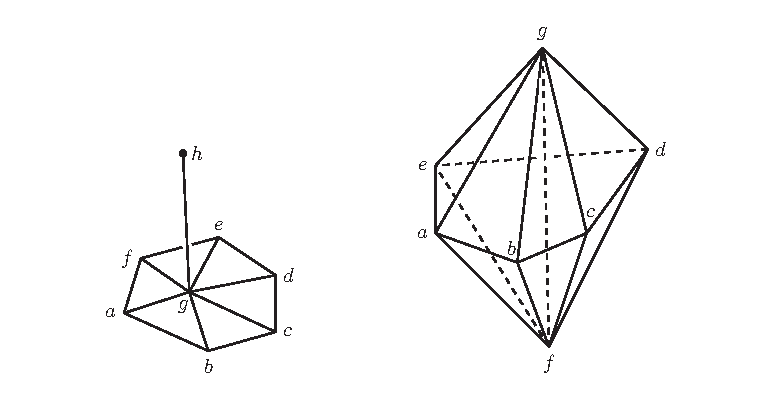
\includegraphics[width=.96\textwidth]{figures/8-2-1-2.pdf}
\caption*{图 8.2.1（左）与图 8.2.2（右）}
\end{figure}

\entry{引理}{8.2.10}设 $s$ 是复形 $K$ 的单形，则
\[
\overline{\operatorname{St}}s=s*\operatorname{Lk}s,\qquad
\overline{\operatorname{St}}s-\operatorname{St}s=\Bd s*\operatorname{Lk}s.
\]
这里把 $s,\Bd s,\operatorname{Lk}s$ 同时看作子空间和子复形。为使链环或边界为空时公式仍成立，约定 $K*\varnothing=\varnothing*K=K$。

\textbf{证明：}第一个等式直接来自定义：闭星形邻域由 $s*t$ 及其面组成，链环由相应的面 $t$ 组成。若一个单形位于闭星形邻域而不在开星形邻域中，它必为某个 $s*t$ 的面 $s'*t'$，其中 $s'$ 是 $s$ 的真面，$t'$ 是 $t$ 的面。因为 $t$ 在链环中，$t'$ 也在链环中，所以 $s'*t'$ 位于 $\Bd s*\operatorname{Lk}s$。反过来，每个这样的单形都在闭星形邻域中而不在开星形邻域中。\hfill$\square$

下面的定义推广定义 8.2.1，将在习题 2 中使用。

\entry{定义}{8.2.11}对拓扑空间 $X,Y$，定义 $X*Y$ 为 $X\times Y\times I$ 的商空间，其中把每个集合 $x\times Y\times0$ 压成一点，把每个 $X\times y\times1$ 压成一点。

\sourcepage{449--450}
\subsection*{习题}
\begin{enumerate}
\item 设 $s$ 是图 8.2.2 中的单形 $fg$。描述 $\widehat s*\operatorname{Lk}s$、$\widehat s*\Bd s$ 以及 $\Bd s*\operatorname{Lk}s$。
\item \begin{enumerate}[label=(\alph*)]
\item 证明 $i(x)=x\times Y\times0$ 和 $j(y)=X\times y\times1$ 分别定义 $X,Y$ 到 $X*Y$ 的嵌入。
\item 若 $X\approx X'$ 且 $Y\approx Y'$，证明 $X*Y\approx X'*Y'$。
\item 证明 $X*Y\approx Y*X$。
\end{enumerate}
\item 〔*〕证明存在分裂短正合列
\[0\to\widetilde H_{p+1}(X*Y)\to\widetilde H_p(X\times Y)
\to\widetilde H_p(X)\oplus\widetilde H_p(Y)\to0.\]
\item 〔*〕证明 $(X*Y)*Z\approx X*(Y*Z)$。〔提示：看似直接的证明并不奏效。下列两组商映射所实施的粘合不同：
\[
(X\times Y\times I_1)\times Z\times I_2\to(X*Y)\times Z\times I_2\to(X*Y)*Z,
\]
\[
X\times(Y\times Z\times I_2)\times I_1\to X\times(Y*Z)\times I_1\to X*(Y*Z).
\]
应在 $X\times Y\times Z\times\Delta_2$ 上引入以下等价关系：
\[
\begin{array}{ll}
(x,y,z,w)\sim(x',y,z,w),&w\in\epsilon_1\epsilon_2,\\
(x,y,z,w)\sim(x,y',z,w),&w\in\epsilon_0\epsilon_2,\\
(x,y,z,w)\sim(x,y,z',w),&w\in\epsilon_0\epsilon_1.
\end{array}
\]
记商空间为 $W$，商映射为 $\pi$。令 $f:I_1\times I_2\to\Delta_2$ 把 $t\times I_2$ 线性映到从 $t\in\epsilon_0\epsilon_1=[0,1]$ 到 $\epsilon_2$ 的线段。证明复合
\[
X\times Y\times Z\times I_1\times I_2
\xrightarrow{\mathrm{id}\times f}X\times Y\times Z\times\Delta_2\xrightarrow{\pi}W
\]
实施的粘合与前面第一组商映射相同，从而 $W\approx(X*Y)*Z$。再证明 $W\approx X*(Y*Z)$。〕
\item 设 $K,L$ 各为一个三角形。它们的联结是什么？
\item 把数字 $8$ 的形状写成两个单形的联结。
\end{enumerate}

\section{同调流形}
\sourcepage{451}
本节定义同调流形，并研究它们的一些局部性质。同调流形包含所有拓扑流形，因此是一类广泛而重要的空间。可三角剖分的同调流形将是各种对偶定理中的基本研究对象。

为方便起见，本节直接讨论相对同调流形，尽管直到第 8.10 节才会真正证明相对情形的对偶定理。

先约定一种记号上的简化。我们所研究的空间都可三角剖分。如果 $X$ 已配有一个特定的三角剖分，常常不在记号上区分空间与剖分它的复形。例如可以说空间 $X$ 的一个点，也可以说复形 $X$ 的一个单形，具体含义由上下文说明。

\entry{定义}{8.3.1}拓扑偶 $(X,A)$ 称为\emph{相对同调 $n$ 维流形}，如果对每个 $x\in X\setminus A$，局部同调群满足
\[
H_i(X,X\setminus\{x\})\cong
\begin{cases}\Z,&i=n,\\0,&i\ne n.\end{cases}
\]
当 $A$ 为空时，简称 $X$ 为\emph{同调 $n$ 维流形}。

若 $M$ 是带边界的 $n$ 维流形，则 $(M,\Bd M)$ 是相对同调 $n$ 维流形（见第 4.8 节）。更一般地，只要 $X\setminus A$ 是 $n$ 维流形，$(X,A)$ 就是相对同调 $n$ 维流形。

若 $(X,A)$ 已三角剖分，则 $X$ 的局部同调性质反映在各单形链环的同调群中。下一引理给出这种联系。

\entry{引理}{8.3.2}设 $s$ 是复形 $K$ 的 $k$ 维单形，$\widehat s$ 是其重心，则
\[
H_i(|K|,|K|\setminus\{\widehat s\})\cong
\begin{cases}
\widetilde H_{i-k-1}(\operatorname{Lk}s),&\operatorname{Lk}s\ne\varnothing,\\
H_i(s,\Bd s),&\operatorname{Lk}s=\varnothing.
\end{cases}
\]

\textbf{证明：}若链环为空，$s$ 不是任何更高维单形的面，所以 $\Int s$ 在 $|K|$ 中开。由切除及 $\Bd s$ 是 $s\setminus\{\widehat s\}$ 的形变收缩核，
\[
H_i(|K|,|K|\setminus\{\widehat s\})\cong H_i(s,s\setminus\{\widehat s\})\cong H_i(s,\Bd s).
\]

若链环非空，因重心位于开集 $\operatorname{St}s$ 中，可切除该开集的补集，得到
\[
H_i(|K|,|K|\setminus\{\widehat s\})\cong
H_i(\overline{\operatorname{St}}s,\overline{\operatorname{St}}s\setminus\{\widehat s\}).
\]
\sourcepage{452}
由凸集的基本性质，$|s|=|\widehat s*\Bd s|$，从而由引理 8.2.10，
\[
|\overline{\operatorname{St}}s|=|s*\operatorname{Lk}s|
=|\widehat s*\Bd s*\operatorname{Lk}s|.
\]
按前述约定，$\Bd s$ 为空时等式仍成立。闭星形邻域是以 $\widehat s$ 为顶点的锥，故无环。从锥中删去顶点后，可以形变收缩到底空间（引理 4.8.12）。因此 $|\Bd s*\operatorname{Lk}s|$ 是删去重心后的闭星形邻域的形变收缩核，故
\begin{align*}
H_i(|K|,|K|\setminus\{\widehat s\})
&\cong H_i(\overline{\operatorname{St}}s,\overline{\operatorname{St}}s\setminus\{\widehat s\})\\
&\cong\widetilde H_{i-1}(\overline{\operatorname{St}}s\setminus\{\widehat s\})\\
&\cong\widetilde H_{i-1}(\Bd s*\operatorname{Lk}s)
\cong\widetilde H_{i-k-1}(\operatorname{Lk}s).
\end{align*}
若 $\Bd s$ 为空，则 $k=0$，最后一个同构就是等同；否则由 $\Bd s$ 是拓扑 $(k-1)$ 维球面及定理 8.2.7 得到。\hfill$\square$

\entry{定理}{8.3.3}设 $(X,A)$ 是已三角剖分的相对同调 $n$ 维流形，$s$ 是不属于 $A$ 的 $k$ 维单形。若链环为空，则 $k=n$；若链环非空，则它具有 $(n-k-1)$ 维球面的同调，其中 $n-k-1\ge0$。两种情形下都有 $k\le n$。

\textbf{证明：}重心 $\widehat s\in X\setminus A$，所以该点的局部同调只在 $n$ 维为无限循环群。链环为空时，上一引理给出非零群 $H_n(s,\Bd s)$，所以 $\dim s=n$。链环非空时，其约化同调只在 $n-k-1$ 维为无限循环群，所以 $n-k-1\ge0$。\hfill$\square$

\entry{推论}{8.3.4}设 $(X,A)$ 是已三角剖分的相对同调 $n$ 维流形。
\begin{enumerate}[label=(\alph*)]
\item $X\setminus A$ 的闭包是一些 $n$ 维单形的并。
\item 不属于 $A$ 的每个 $(n-1)$ 维单形恰好是两个 $n$ 维单形的面。
\end{enumerate}

\textbf{证明：}(a) 若 $s\notin A$ 且 $\dim s=k$，则 $k\le n$。若 $k<n$，其链环是同调 $(n-k-1)$ 维球面，因而含有一个 $(n-k-1)$ 维单形 $t$，于是 $s$ 是 $n$ 维单形 $s*t$ 的面。

(b) 对不属于 $A$ 的 $(n-1)$ 维单形 $s$，其链环具有零维球面的同调。由于闭星形邻域维数为 $n$，且等于 $s*\operatorname{Lk}s$，链环必为零维。因此它恰由两个点组成，对应恰好两个 $n$ 维单形。\hfill$\square$

\sourcepage{453}
上述结果说明，已三角剖分的相对同调 $n$ 维流形满足相对伪流形定义的前两个条件（定义 5.4.5）。若 $X\setminus A$ 连通，也满足第三个条件。证明提纲见本节习题；以后也会由对偶定理推导这一事实。

\entry{例}{8.3.5}设 $X$ 是环面 $T$ 与二维球面 $S^2$ 的不交并，$S(X)$ 是其悬挂，$A=\{w_0,w_1\}$ 是两个悬挂点（图 8.3.1）。则 $(S(X),A)$ 是相对同调三维流形，因为 $S(X)\setminus A\approx X\times(-1,1)$ 是三维流形。

子空间偶 $(S(T),A)$ 和 $(S(S^2),A)$ 也都是相对同调三维流形，而且是相对伪三维流形。$S(S^2)$ 是同调三维流形，$S(T)$ 则不是，因为后者中 $w_0$ 的链环是环面，而不是同调二维球面。

\begin{figure}[htbp]\centering
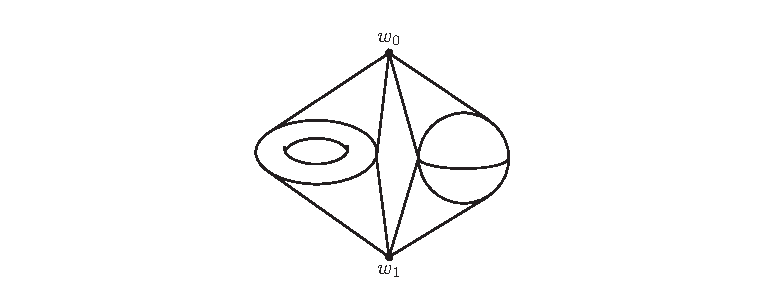
\includegraphics[width=.85\textwidth]{figures/8-3-1.pdf}
\caption*{图 8.3.1}
\end{figure}

\entry{例}{8.3.6}通常所画的流形图形，可能使人猜想：若 $M$ 是已三角剖分的拓扑 $n$ 维流形，则每个 $k$ 维单形的链环都是拓扑 $(n-k-1)$ 维球面。

对通常的二维流形三角剖分，这当然成立：例如边的链环是零维球面，顶点的链环是一维球面。这个猜想长期悬而未决，直到 Robert D. Edwards 和 James W. Cannon 的工作才得到解决（见 [Can79]）。细节较复杂，此处从略。

\entry{例}{8.3.7}确实存在不是拓扑流形的同调 $n$ 维流形。下面概述一种构造，但证明要用到尚未学习的工具。

\sourcepage{454}
所需的基本事实是：存在紧致、已三角剖分的三维流形 $M$，它是同调三维球面，但基本群 $\pi_1(M)$ 不为零。其构造见 [ST80]。原文称其基本群为二十面体群。\translatornote{通常这里的 Poincaré 同调球面的基本群是二元二十面体群；它与普通二十面体旋转群不同。}

取悬挂 $S(M)=M*\{w_0,w_1\}$，则它是同调四维流形。因为除去悬挂点后同胚于四维流形 $M\times(-1,1)$，局部同调条件在其他所有点成立；又因为两个悬挂点的链环均为同调三维球面 $M$，条件在悬挂点也成立。

还需另行证明：在已三角剖分的拓扑 $n$ 维流形中，每个顶点的链环即使不一定同胚于 $(n-1)$ 维球面，也必须具有该球面的同伦型。由于 $\pi_1(M)\ne0$，$M$ 不具有三维球面的同伦型，所以 $S(M)$ 不可能是拓扑四维流形。

以下定理和推论留作习题。

\entry{定理}{8.3.8}若 $(X,A)$ 是已三角剖分的相对同调 $n$ 维流形，且 $X\setminus A$ 连通，则 $(X,A)$ 是相对伪 $n$ 维流形。

\entry{推论}{8.3.9}若 $(X,A)$ 是已三角剖分的相对同调 $n$ 维流形，$s$ 是不属于 $A$ 的单形，则 $\operatorname{Lk}s$ 是有限复形。

\sourcepage{454--455}
\subsection*{习题}
前四题每一题都依赖于前面的习题。
\begin{enumerate}
\item 设 $(X,A)$ 是已三角剖分的拓扑偶。假定对每个不属于 $A$ 的 $k$ 维单形 $s$ 都有：(i) $k\le n$；(ii) 若 $k<n$，则 $H_i(\operatorname{Lk}s)\cong H_i(S^{n-k-1})$。证明 $(X,A)$ 是相对同调 $n$ 维流形。
\item 设 $(X,A)$ 是已三角剖分的相对同调 $n$ 维流形。若 $s\notin A$ 且 $\dim s=k<n$，证明 $\operatorname{Lk}s$ 是同调 $(n-k-1)$ 维流形。〔提示：把链环看作 $X$ 的子复形。对 $t\in\operatorname{Lk}s$，证明
\[\operatorname{Lk}(t,\operatorname{Lk}(s,X))=\operatorname{Lk}(t*s,X).\]〕
\item 证明定理 8.3.8。〔提示：$n=1$ 时显然。假设对小于 $n$ 的维数成立。若存在不属于 $A$ 的 $n$ 维单形序列
\[\sigma=\sigma_0,\sigma_1,\ldots,\sigma_k=\sigma',\]
使每个 $\sigma_i\cap\sigma_{i+1}$ 都是不属于 $A$ 的 $(n-1)$ 维单形，就定义 $\sigma\sim\sigma'$。令 $X_1$ 是一个等价类中元素的并，$X_2$ 是其他等价类中元素的并。若 $s\notin A$ 且 $s\subset X_1\cap X_2$，记 $k=\dim s$，则 $k<n-1$。证明 $\operatorname{Lk}s$ 是伪 $(n-k-1)$ 维流形，进而闭星形邻域中任意两个 $n$ 维单形都等价。〕\translatornote{原文提示中相邻单形下标及“对每个 $i$”有排印错误，此处按相邻关系写出。}
\item 证明推论 8.3.9。〔提示：若 $X$ 是伪 $m$ 维流形且 $H_m(X)\ne0$，则 $X$ 必有限。〕
\item 能否举出第一项空间 $X$ 为圆的相对同调 $n$ 维流形？为什么？
\item 能否举出第一项空间 $X$ 为二维球面的相对同调 $n$ 维流形？为什么？
\end{enumerate}

\section{对偶块复形}
\sourcepage{455--456}
为简便起见，接下来几节先只讨论同调 $n$ 维流形 $X$。所用方法以后还将在相对同调流形的情形中出现。

对于已三角剖分的同调流形，可以把 $X$ 分成一些“几乎”是开胞腔的子集，使其“几乎”成为正则胞腔复形。这些子集不是实际的拓扑胞腔，而只是同调意义的胞腔，因此称它们为\emph{块}，并称所得分解为 $X$ 的\emph{对偶块分解}。与胞腔复形一样，块复形也有一个可用于计算 $X$ 同调和上同调的链复形，称为\emph{对偶链复形}。这是证明对偶定理的关键工具。

回顾第 2.3 节，$\sigma_1\succ\sigma_2$ 表示 $\sigma_2$ 是 $\sigma_1$ 的真面。

\entry{定义}{8.4.1}设 $X$ 是局部有限单纯复形，$\operatorname{sd}X$ 为第一次重心重分。由引理 2.3.9，其单形形如
\[
\widehat\sigma_{i_1}\widehat\sigma_{i_2}\cdots\widehat\sigma_{i_k},
\qquad\sigma_{i_1}\succ\sigma_{i_2}\succ\cdots\succ\sigma_{i_k}.
\]
始终按此顺序排列顶点。为便于记录，称第一个顶点为该单形的\emph{最大顶点}，最后一个为\emph{最小顶点}。

\entry{例}{8.4.2}设 $X$ 是平面中顶点为 $a,b,c$ 的三角区域，视为二维单纯复形。其重心重分的顶点为
\[a,b,c,\quad\widehat{ab},\widehat{bc},\widehat{ca},\quad\widehat{abc}.\]
顶点 $\widehat{abc}$ 在任何包含它的单形中都是最大顶点；以它为最小顶点的单形只有它自身。$\widehat{ab}$ 是边 $\widehat{ab}a,\widehat{ab}b$ 以及零维单形 $\widehat{ab}$ 的最大顶点，也是边 $\widehat{abc}\widehat{ab}$ 以及它自身的最小顶点。

\entry{定义}{8.4.3}给定 $X$ 的单形 $\sigma$，注意以 $\widehat\sigma$ 为最大顶点的所有重分后开单形的并恰为 $\Int\sigma$。另一方面，定义 $D(\sigma)$ 为以 $\widehat\sigma$ 为最小顶点的所有开单形之并，称为\emph{与 $\sigma$ 对偶的块}。

这些块起到类似 CW 复形开胞腔的作用。其闭包 $\overline D(\sigma)$ 称为\emph{对偶闭块}，是所有末顶点为 $\widehat\sigma$ 的单形及其面的并，因而是 $\operatorname{sd}X$ 的子复形的多面体。记
\[\dot D(\sigma)=\overline D(\sigma)\setminus D(\sigma).\]

\begin{figure}[htbp]\centering
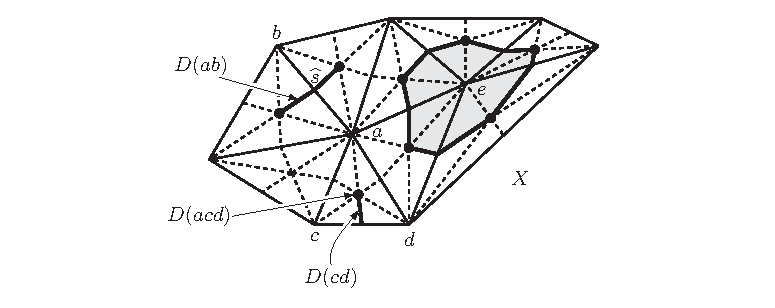
\includegraphics[width=.88\textwidth]{figures/8-4-1.pdf}
\caption*{图 8.4.1}
\end{figure}

\entry{例}{8.4.4}设 $X$ 为图 8.4.1 的二维复形，虚线表示其重心重分。每个二维单形的对偶块只有其重心。边 $s=ab$ 的对偶块由重心 $\widehat s$，以及从它连接到以该边为面的两个三角形重心的两条开线段组成。顶点 $e$ 的对偶块是图中的阴影区域，相应闭块还包括该区域边界。值得注意的是，$\dot D(e)$ 是所有以 $e$ 为面的边和三角形所对应的低维对偶块之并。我们很快就会证明这普遍成立。

\sourcepage{457}
\entry{例}{8.4.5}图 8.4.2 的复形是四边形 $cdefc$ 与线段 $ab$ 的联结。读者可以想象其重心重分。每个三维单形的对偶块是其重心。三角形 $abc$ 的对偶闭块由两条线段组成，连接该三角形重心与以它为面的两个三维单形的重心。边 $ab$ 的对偶闭块是图 8.4.3 的闭八边形区域；$\dot D(ab)$ 为其边界，是所有以 $ab$ 为面的二维、三维单形的对偶块之并。

\begin{figure}[htbp]\centering
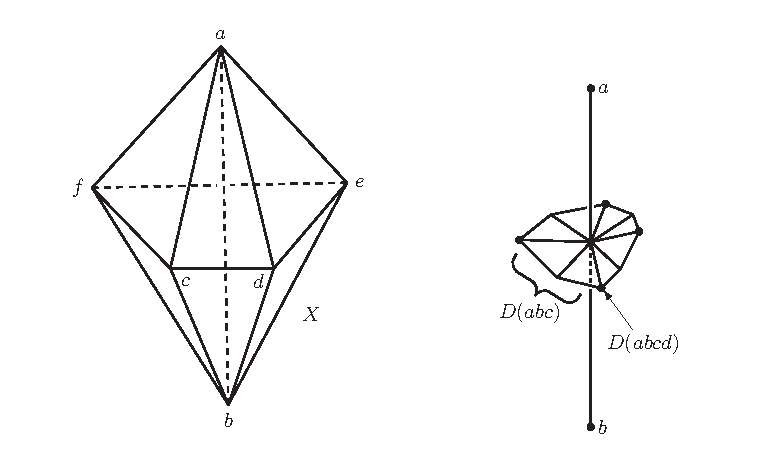
\includegraphics[width=.96\textwidth]{figures/8-4-2-3.pdf}
\caption*{图 8.4.2（左）与图 8.4.3（右）}
\end{figure}

证明下一定理时，请记住这两个例子。

\entry{定理}{8.4.6}设 $X$ 是局部有限单纯复形，完全由 $n$ 维单形及其面组成，$\sigma$ 是其中一个 $k$ 维单形。则：
\begin{enumerate}[label=(\alph*)]
\item 各对偶块不交，其并为 $|X|$。
\item $\overline D(\sigma)$ 是 $\operatorname{sd}X$ 的一个 $(n-k)$ 维子复形的多面体。
\item $\dot D(\sigma)$ 是所有满足 $\tau\succ\sigma$ 的块 $D(\tau)$ 的并；这些块的维数均小于 $n-k$。
\item $\overline D(\sigma)=|\dot D(\sigma)*\widehat\sigma|$。
\item 若 $\widehat\sigma$ 处局部同调只在 $n$ 维为 $\Z$，则 $(\overline D(\sigma),\dot D(\sigma))$ 具有 $(n-k)$ 维胞腔模其边界的同调。
\end{enumerate}

\textbf{证明：}(a) 重分后的开单形两两不交，每个恰位于一个块中，即其最小顶点所对应的块。

\sourcepage{458}
(b) 取以 $\sigma$ 为面的 $n$ 维单形 $\sigma'$，可以找到逐次降低一维的面链
\[\sigma'=\sigma_n\succ\sigma_{n-1}\succ\cdots\succ\sigma_k=\sigma.\]
由这些重心组成的重分后单形维数为 $n-k$，且位于 $\overline D(\sigma)$ 中。由于 $X$ 没有高于 $n$ 维的单形，以 $\widehat\sigma$ 为末顶点的单形不可能有更高维数。

(c)、(d) 闭块由所有形如
\[\widehat\sigma_{i_1}\cdots\widehat\sigma_{i_p}\widehat\sigma\]
的单形及其面组成。这样的单形与 $\dot D(\sigma)$ 的交，是删去末顶点所得的面。因此 $\dot D(\sigma)$ 由所有满足 $\sigma_{i_p}\succ\sigma$ 的单形 $\widehat\sigma_{i_1}\cdots\widehat\sigma_{i_p}$ 组成，其内部恰位于 $D(\sigma_{i_p})$ 中。反之，这些块中的每个开单形都有此形式。于是得到 (c)，同时也得到锥的描述 (d)。

(e) 若 $k=n$，闭块只有重心，是零维胞腔。设 $k<n$。在重分复形中，$\widehat\sigma$ 的闭星形邻域由顶点面链中包含 $\sigma$ 的所有单形组成。在面链中位于 $\sigma$ 之前的部分组成 $\dot D(\sigma)$ 的单形，$\sigma$ 及其后的部分组成 $\operatorname{sd}\sigma$ 的单形。因此
\[
\overline{\operatorname{St}}(\widehat\sigma,\operatorname{sd}X)
=\dot D(\sigma)*\operatorname{sd}\sigma
=\dot D(\sigma)*\widehat\sigma*\operatorname{sd}(\Bd\sigma).
\]
另一方面，闭星形邻域等于 $\widehat\sigma*\operatorname{Lk}(\widehat\sigma,\operatorname{sd}X)$，所以
\[\operatorname{Lk}(\widehat\sigma,\operatorname{sd}X)=\dot D(\sigma)*\operatorname{sd}(\Bd\sigma).\]
由于 $\operatorname{sd}(\Bd\sigma)$ 是拓扑 $(k-1)$ 维球面（$k=0$ 时为空），
\[\widetilde H_{i+k}(\operatorname{Lk}(\widehat\sigma,\operatorname{sd}X))\cong\widetilde H_i(\dot D(\sigma)).\]
\sourcepage{459}
由局部同调假设及引理 8.3.2，左侧链环是同调 $(n-1)$ 维球面，故 $\dot D(\sigma)$ 是同调 $(n-k-1)$ 维球面。闭块为锥，故无环，其同调长正合列给出
\[H_i(\overline D(\sigma),\dot D(\sigma))\cong\widetilde H_{i-1}(\dot D(\sigma)),\]
于是得到胞腔模边界的同调。\hfill$\square$

\entry{定义}{8.4.7}设 $X$ 是局部有限的同调 $n$ 维流形复形。\footnote{事实上，每个作为同调 $n$ 维流形的复形都是局部有限的。}上一定理适用于每个单形。所有对偶块组成 $X$ 的\emph{对偶块分解}。维数不超过 $p$ 的块之并记作 $X_p$，称为\emph{对偶 $p$ 维骨架}。定义\emph{对偶链复形} $\mathcal D(X)$：
\[\mathcal D_p(X)=H_p(X_p,X_{p-1}),\]
边缘算子为三元组 $(X_p,X_{p-1},X_{p-2})$ 的正合列中的连接同态 $\partial_*$。

对偶骨架是 $\operatorname{sd}X$ 的子复形的多面体，因而有时把它直接视为复形。特别地，为方便起见，定义 $\mathcal D_p(X)$ 时采用单纯同调。

对偶链复形在计算同调和上同调中的作用，实际上与 CW 复形的胞腔链复形相同。仿照第 4.13 节，得到如下结论。

\entry{定理}{8.4.8}设 $X$ 是局部有限的同调 $n$ 维流形复形，$X_p$ 为对偶骨架。
\begin{enumerate}[label=(\alph*)]
\item $H_i(X_p,X_{p-1})$ 在 $i\ne p$ 时为零，$i=p$ 时为自由阿贝尔群。一组基可以如下取得：对每个 $p$ 维块，选取 $H_p(\overline D(\sigma),\dot D(\sigma))$ 的生成元，再取其在包含映射诱导的同态下的像。
\item $\mathcal D(X)$ 可用于计算 $X$ 的同调。确切地说，$\mathcal D_p(X)$ 可等同于 $C_p(\operatorname{sd}X)$ 中承载于 $X_p$ 且边界承载于 $X_{p-1}$ 的链所组成的子群。包含映射诱导同调同构，因而也诱导任意系数的同调和上同调同构。\translatornote{原文这句把链的承载空间写为 $X$；按定义应为对偶骨架 $X_p$。}
\end{enumerate}

\sourcepage{460}
\textbf{证明：}(a) 仿照引理 4.13.4，但更为简单。每个闭块是以 $\widehat\sigma$ 为顶点的锥，删去顶点后可形变收缩到 $\dot D(\sigma)$。这些形变收缩合起来，给出
\[X_p\setminus\bigcup_p\{\widehat\sigma\}\longrightarrow X_{p-1}\]
的形变收缩，其中并集遍历所有 $(n-p)$ 维单形的重心。考虑所有 $p$ 维闭块偶的拓扑和。先把每个偶 $(\overline D(\sigma),\dot D(\sigma))$ 的第二项扩大为删去重心的闭块；由形变收缩，诱导同调同构。将拓扑和映入 $(X_p,X_p\setminus\bigcup_p\{\widehat\sigma\})$，再由切除得到各局部部分的同调直和。对应的包含映射给出交换图，并得到
\[
\bigoplus_{\dim D(\sigma)=p}H_i(\overline D(\sigma),\dot D(\sigma))
\cong H_i(X_p,X_{p-1}).
\]
于是 (a) 对奇异同调成立，因而也对单纯同调成立。(b) 直接由定理 4.13.9 得到。\hfill$\square$

我们现已具备证明 Poincaré 对偶定理的基本工具。

\sourcepage{460--461}
\subsection*{习题}
\begin{enumerate}
\item 考虑环面 $T$ 的通常三角剖分。
\begin{enumerate}[label=(\alph*)]
\item 画出对偶块分解。注意这些块实际上使 $T$ 成为正则胞腔复形。
\item 设 $C(T)$ 为单纯链复形，$\mathcal D(T)$ 为对偶链复形。把二维单形逆时针定向，边任意定向。对每个有向二维单形，令
\[\varphi:C^2(T)\to\mathcal D_0(T),\qquad\varphi(\sigma^*)=D(\sigma)=\widehat\sigma.\]
再定义同构 $\varphi:C^1(T)\to\mathcal D_1(T)$，使 $\varphi(e^*)$ 为 $(\overline D(e),\dot D(e))$ 的一个基本闭链。证明可以选择这些基本闭链，使 $\partial\varphi(e^*)=\varphi(\delta e^*)$。
\item 定义 $\varphi:C^0(T)\to\mathcal D_2(T)$，使 $\varphi(v^*)$ 为 $(\overline D(v),\dot D(v))$ 的基本闭链。证明若二维胞腔 $D(v)$ 逆时针定向，则 $\partial\varphi(v^*)=\varphi(\delta v^*)$。
\item 得出对所有 $p$ 都有 $H^p(T)\cong H_{2-p}(T)$（这一点我们已经知道）。
\end{enumerate}
这道习题展示了 Poincaré 对偶的证明方法。
\item 对 Klein 瓶重复习题 1，同调和上同调都取 $\Z/2$ 系数。注意不涉及符号，所以证明更容易。
\item 若把前两题中的环面和 Klein 瓶换成球面，可以得到什么结论？
\item 若把前两题中的对象换成双环面（有两个孔），可以得到什么结论？
\end{enumerate}

\section{Poincaré 对偶}
\sourcepage{461--462}
Poincaré 对偶定理是整个拓扑学中最深刻的结果之一。它最初表述为：对紧致、可定向、已三角剖分的 $n$ 维流形，$k$ 维与 $(n-k)$ 维的 Betti 数相等，$k$ 维与 $(n-k-1)$ 维的挠系数相同。现代通常使用另一种等价表述：$k$ 维上同调群与 $(n-k)$ 维同调群同构。

当空间不可定向或非紧时，也有相应版本，我们也将讨论。这里给出两种证明。本节的第一个证明直接而直观；第 8.7 节的第二个证明还将说明对偶同构在连续映射下的行为，并提供流形杯积的信息。

\entry{定义}{8.5.1}设 $X$ 是紧致、已三角剖分的同调 $n$ 维流形。若能给所有 $n$ 维单形 $\sigma_i$ 定向，使其和 $\gamma=\sum\sigma_i$ 为闭链，则称 $X$ \emph{可定向}，并称 $\gamma$ 为\emph{定向闭链}。

若 $X$ 非紧，但剖分复形局部有限，同样允许这个和为无限链。若无法这样选择定向，则称 $X$ \emph{不可定向}。

若 $X$ 不连通，其每个分支仍是同调 $n$ 维流形。$X$ 可定向当且仅当各分支都可定向，各分支的定向闭链之和为 $X$ 的定向闭链。我们将证明可定向性不依赖于具体三角剖分（推论 8.5.5）。

\entry{定理}{8.5.2（Poincaré 对偶——第一种形式）}设 $X$ 是紧致、已三角剖分的同调 $n$ 维流形。若 $X$ 可定向，则对任意系数群 $G$ 及所有 $p$，
\[H^p(X;G)\cong H_{n-p}(X;G).\]
若 $X$ 不可定向，则对所有 $p$，
\[H^p(X;\Z/2)\cong H_{n-p}(X;\Z/2).\]

\textbf{证明：}用单纯链复形计算上同调，用对偶链复形计算同调。$p$ 维单形与其 $(n-p)$ 维对偶块一一对应，所以自由阿贝尔群 $C^p(X)$ 与 $\mathcal D_{n-p}(X)$ 同构：把有向单形的对偶基元 $\sigma^*$ 映到 $H_{n-p}(\overline D(\sigma),\dot D(\sigma))$ 的一个生成元。若 $X$ 可定向，我们将选取这些生成元的符号，使同构 $\varphi$ 满足
\[\partial\varphi=\varphi\delta:C^{p-1}(X)\longrightarrow\mathcal D_{n-p}(X).\]
这就证明整数系数情形。

先给所有 $n$ 维单形定向，使其和为定向闭链；其他维单形任意定向。从 $n$ 维开始，令
\[\varphi:C^n(X)\to\mathcal D_0(X),\qquad\varphi(\sigma^*)=\widehat\sigma.\]
因为重心生成 $H_0(\widehat\sigma)$，这是同构。

\sourcepage{463}
接着在 $n-1$ 维定义。设 $s$ 是有向 $(n-1)$ 维单形，它恰为两个 $n$ 维单形 $\sigma_0,\sigma_1$ 的面。定向闭链的边界为零，因此可编号使 $\partial\sigma_0$ 在 $s$ 上的系数为 $-1$，$\partial\sigma_1$ 的系数为 $1$。于是
\[\delta s^*=\sigma_1^*-\sigma_0^*,\qquad
\varphi(\delta s^*)=\widehat\sigma_1-\widehat\sigma_0.\]
定义
\[\varphi(s^*)=[\widehat\sigma_0,\widehat s]+[\widehat s,\widehat\sigma_1].\]
这就是一维对偶块模边界的基本闭链，且 $\partial\varphi(s^*)=\varphi(\delta s^*)$。

\begin{figure}[htbp]\centering
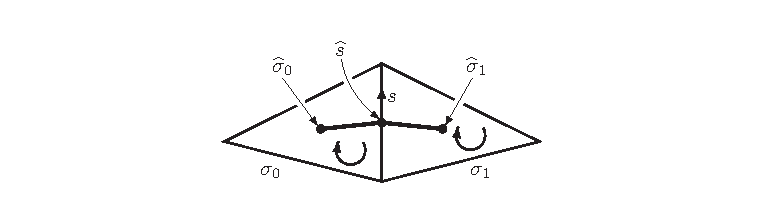
\includegraphics[width=.85\textwidth]{figures/8-5-1.pdf}
\caption*{图 8.5.1}
\end{figure}

一般地，设已在 $p+1<n$ 维及以上定义 $\varphi$，现在要使每个有向 $p$ 维单形满足同样的边缘关系。写
\[\delta s^*=\sum\epsilon_i\sigma_i^*,\qquad
\varphi(\delta s^*)=\sum\epsilon_i\varphi(\sigma_i^*),\]
其中遍历所有以 $s$ 为面的 $(p+1)$ 维单形，$\epsilon_i=\pm1$ 是 $\partial\sigma_i$ 在 $s$ 上的系数。我们证明后一链是 $\dot D(s)$ 的基本闭链。

\sourcepage{464}
每个 $\varphi(\sigma_i^*)$ 是相应对偶块模其边界的基本闭链，且该块位于 $\dot D(s)$ 中。因此总和承载于 $\dot D(s)$；由归纳假设，
\[\partial\varphi(\delta s^*)=\varphi(\delta\delta s^*)=0.\]
而 $\dot D(s)$ 是同调 $(n-p-1)$ 维球面，其中 $n-p-1>0$。这个闭链非零，且不是另一个闭链的非平凡整数倍，因为把它限制到任一对应块，所得链（差一个符号）是该块模边界的基本闭链。因此它代表 $H_{n-p-1}(\dot D(s))$ 的生成元。

考虑正合列
\[0\to H_{n-p}(\overline D(s),\dot D(s))\xrightarrow{\partial_*}
H_{n-p-1}(\dot D(s))\to0.\]
由于维数原因，这里的同调群可以等同于相应闭链群。令 $\varphi(s^*)$ 为边界恰等于 $\varphi(\delta s^*)$ 的基本相对闭链，就完成了归纳定义。

于是整数系数情形得证。对任意系数，使用同构
\[
\operatorname{Hom}(C_p(X),G)\cong\operatorname{Hom}(C_p(X),\Z)\otimes G
\xrightarrow{\varphi\otimes i_G}\mathcal D_{n-p}(X)\otimes G.
\]
它们与 $\delta,\partial$ 交换，第一个同构已在定理 7.6.1 第二步证明。

最后考虑不可定向情形。相同证明在 $\Z/2$ 上成立，归纳定义
\[\operatorname{Hom}(C_p(X),\Z/2)\xrightarrow{\varphi}\mathcal D_{n-p}(X)\otimes\Z/2.\]
对 $n$ 维单形，令 $\sigma^*$ 在该单形上取 $[1]$，其他单形上取零，并置 $\varphi(\sigma^*)=\widehat\sigma\otimes[1]$。对 $(n-1)$ 维单形令
\[\varphi(s^*)=\bigl([\widehat\sigma_0,\widehat s]+[\widehat s,\widehat\sigma_1]\bigr)\otimes[1].\]
系数为 $\Z/2$，符号无关紧要。其余证明不变，只需将“基本闭链”替换为“$\Z/2$ 系数的唯一非零闭链”。\translatornote{原文在零维起始定义中把 $\widehat\sigma$ 误印为 $\partial$，此处按构造写出。}\hfill$\square$

这里选择单纯复形计算上同调、对偶复形计算同调，并无特殊必要，也可以反过来。$\varphi$ 为同构，所以其对偶同样是同构
\[
\operatorname{Hom}(\mathcal D_{n-p}(X),\Z)
\xrightarrow{\overline\varphi}\operatorname{Hom}(\operatorname{Hom}(C_p(X),\Z),\Z).
\]
再使用自然双对偶同构 $C_p(X)\cong\operatorname{Hom}(\operatorname{Hom}(C_p(X),\Z),\Z)$，它把 $\partial$ 对应到 $\delta$ 的对偶（定理 7.6.1 第四步），就得到与边缘、上边缘交换的同构
\[\operatorname{Hom}(\mathcal D_{n-p}(X),\Z)\cong C_p(X).\]

\sourcepage{465}
\entry{推论}{8.5.3}若 $X$ 是紧致连通、已三角剖分的同调 $n$ 维流形，则任意两个 $n$ 维单形之间都可用有限序列
\[\sigma=\sigma_0,\sigma_1,\ldots,\sigma_k=\sigma'\]
相连，其中相邻单形的交为 $(n-1)$ 维单形。

\textbf{证明：}以存在上述序列定义等价关系。每个等价类中的全部 $n$ 维单形之和是 $\Z/2$ 系数闭链，因为任意 $(n-1)$ 维单形所邻接的两个顶维单形属于同一类，故在该和中同时出现或同时不出现。若有多个等价类，就有多个独立的非零顶维闭链，与
\[H_n(X;\Z/2)\cong H^0(X;\Z/2)\cong\Z/2\]
矛盾。\hfill$\square$

结合推论 8.3.4，这也说明紧致连通、已三角剖分的同调流形是伪流形。

\entry{推论}{8.5.4}若上述 $X$ 连通，则可定向时 $H_n(X)\cong\Z$，不可定向时 $H_n(X)=0$。

\textbf{证明：}可定向时由对偶，$H_n(X)\cong H^0(X)\cong\Z$。反之，设有非零整数 $n$ 维闭链 $z$。任意给顶维单形定向，相邻单形在 $z$ 中的系数绝对值必相同，否则边界在公共面上不为零。由上一推论，所有顶维系数都具有同一绝对值 $m>0$。将 $z$ 除以 $m$ 就得到定向闭链。\hfill$\square$

\entry{推论}{8.5.5}紧致、已三角剖分的同调 $n$ 维流形 $X$ 可定向，当且仅当每个分支 $X_i$ 都满足 $H_n(X_i)\cong\Z$。因此可定向性与三角剖分无关。

下一个推论用到上一章的泛系数定理。

\sourcepage{466--467}
\entry{推论}{8.5.6}设 $X$ 是紧致连通、已三角剖分的同调 $n$ 维流形。
\begin{enumerate}[label=(\alph*)]
\item 若可定向，则 $H_{n-1}(X)$ 无挠，且对任意 $G$，
\[H_n(X;G)\cong G\cong H^n(X;G).\]
\item 若不可定向，则 $H_{n-1}(X)$ 的挠子群阶为 $2$，且
\[H_n(X;G)\cong\ker\varphi_2,\qquad H^n(X;G)\cong G/2G,\]
其中 $\varphi_2:G\to G$ 为乘以 $2$ 的同态。特别地，$H_n(X)=0$，$H^n(X)\cong\Z/2$。
\end{enumerate}

\textbf{证明：}(a) 由对偶，$H_n(X;G)\cong H^0(X;G)$，$H^n(X;G)\cong H_0(X;G)$；连通性使两个零维群都同构于 $G$。又由泛系数定理，
\[H^n(X)\cong\operatorname{Hom}(H_n(X),\Z)\oplus\operatorname{Ext}(H_{n-1}(X),\Z).\]
左端与第一项均为 $\Z$，而第二项同构于 $H_{n-1}(X)$ 的挠子群（定理 7.2.5），所以该挠子群为零。

(b) 任意给顶维单形定向。若 $g\in G$ 满足 $2g=0$，则 $\sum g\sigma_i$ 为闭链，因为每个余维一面恰好邻接两个顶维单形。反之，若 $z$ 是非零 $G$ 系数顶维闭链，在某个顶维单形上的系数为 $g$，则相邻单形上的系数必为 $\pm g$。由推论 8.5.3，
\[z=g\left(\sum\epsilon_i\sigma_i\right),\qquad\epsilon_i=\pm1.\]
括号内的整数链不能是闭链，否则 $X$ 可定向。因此其边界在某个余维一面上的系数非零；该系数必为 $\pm2$。因 $z$ 是闭链，得到 $2g=0$。于是 $g=-g$，所以 $z=\sum g\sigma_i$。顶维没有边界链，因此 $H_n(X;G)\cong\ker\varphi_2$。

令 $T_{n-1}(X)$ 为 $H_{n-1}(X)$ 的挠子群。由于 $H_n(X)=0$，同调泛系数定理给出
\[T_{n-1}(X)*G\cong H_{n-1}(X)*G\cong\ker\varphi_2\cong(\Z/2)*G.\]
特别地，
\[T_{n-1}(X)*\Z/m\cong
\begin{cases}0,&m\text{ 为奇数},\\\Z/2,&m\text{ 为偶数}.\end{cases}\]
因此不存在奇挠系数（令 $m$ 等于该奇数），只能有一个偶挠系数（令 $m=2$），且该系数不可能大于 $2$（令 $m$ 等于该系数）。所以 $T_{n-1}(X)\cong\Z/2$。最后由上同调泛系数定理，
\[H^n(X;G)\cong\operatorname{Ext}(H_{n-1}(X),G)\cong G/2G.\]
\hfill$\square$

\entry{定义}{8.5.7}设同调 $n$ 维流形 $X$ 不一定紧致，但有局部有限的三角剖分。若能给所有顶维单形定向，使可能无限的和 $\sum\sigma_i$ 成为闭链，则称其可定向。

\entry{定理}{8.5.8（Poincaré 对偶——非紧情形）}设 $X$ 是由局部有限复形三角剖分的同调 $n$ 维流形。
\begin{enumerate}[label=(\arabic*)]
\item 对所有 $p$，都有
\[H_c^p(X;\Z/2)\cong H_{n-p}(X;\Z/2),\qquad
H^p(X;\Z/2)\cong H_{n-p}^{\infty}(X;\Z/2).\]
这里 $H_c^p$ 是紧支集上同调（定义 5.5.4），$H_*^{\infty}$ 是无限链同调（定义 1.6.14）。
\item 若 $X$ 可定向，则对任意 $G$ 及所有 $p$，
\[H_c^p(X;G)\cong H_{n-p}(X;G),\qquad
H^p(X;G)\cong H_{n-p}^{\infty}(X;G).\]
\end{enumerate}

\sourcepage{467--468}
\subsection*{习题}
\begin{enumerate}
\item 设 $M,N$ 是紧致连通、可三角剖分的 $n$ 维流形，$f:M\to N$。证明若 $M$ 可定向、$N$ 不可定向，则
\[f_*:H_n(M;\Z/2)\to H_n(N;\Z/2)\]
为零同态。
\item 设 $X$ 是紧致可定向、可三角剖分的流形，第 $i$ 个 Betti 数为 $\beta_i(X)$。回顾 Euler 数公式 $\chi(X)=\sum_i(-1)^i\beta_i(X)$。
\begin{enumerate}[label=(\alph*)]
\item 若 $\dim X$ 为奇数，证明 $\chi(X)=0$。
\item 若 $\dim X=2k$，用 $i\le k$ 的 Betti 数表示 $\chi(X)$。
\item 给出关于切向量场的应用（见第 2.10 节习题 5）。
\end{enumerate}
\item 设 $X$ 是有局部有限三角剖分的同调 $n$ 维流形，不一定紧致。
\begin{enumerate}[label=(\alph*)]
\item 证明定理 8.5.8(1)。
\item 若 $X$ 连通，证明它是伪 $n$ 维流形。
\item 证明定理 8.5.8(2)，并得出可定向性仅依赖于底层拓扑空间，而与具体剖分无关。
\end{enumerate}
\item 证明 Klein 瓶不可定向。
\item 在拓扑教材或互联网上查阅“交叉帽”（cross cap），证明它不可定向。
\end{enumerate}

\section{帽积}
\sourcepage{468--469}
为给出 Poincaré 对偶的第二种证明，先讨论一个纯代数性质的运算，称为上同调类与同调类的\emph{帽积}（cap product）。其定义形式类似第 5.9 节的杯积。它与对偶定理的联系将很快表明其用途。以下 $R$ 为有单位元的交换环。

\entry{定义}{8.6.1}设 $X$ 是拓扑空间。定义
\[\mathcal S^p(X;R)\otimes\mathcal S_{p+q}(X;R)\xrightarrow{\frown}\mathcal S_q(X;R)\]
如下：若 $T:\Delta_{p+q}\to X$ 为奇异单形，$a\in R$，令
\[
c^p\frown(T\otimes a)=T\ell(\epsilon_0,\ldots,\epsilon_q)
\otimes a\langle c^p,T\ell(\epsilon_q,\ldots,\epsilon_{p+q})\rangle.
\]
所得链称为上链 $c^p$ 与链 $T\otimes a$ 的帽积。大致说，就是取 $T$ 在前 $q$ 维面上的限制，系数为 $a$ 乘以上链在后 $p$ 维面上的值。

与杯积一样，也有其他系数版本，包括
\[
\mathcal S^p(X;G)\otimes\mathcal S_{p+q}(X;\Z)\to\mathcal S_q(X;G),\qquad
\mathcal S^p(X;F)\otimes\mathcal S_{p+q}(X;F)\to\mathcal S_q(X;F),
\]
其中 $G$ 为阿贝尔群，$F$ 为域，均由同一公式给出，后面也会用到。

\entry{定理}{8.6.2}帽积双线性，且相对于连续映射自然。它满足边缘公式
\[\partial(d^p\frown c_{p+q})=(-1)^q\delta d^p\frown c_{p+q}+d^p\frown\partial c_{p+q},\]
并与杯积满足关系
\[c^p\frown(d^q\frown e_{p+q+r})=(c^p\smile d^q)\frown e_{p+q+r}.\]

\textbf{证明：}双线性容易检验。自然性表述起来比证明更复杂。对连续映射 $f:X\to Y$、$c^p\in\mathcal S^p(Y)$ 和 $d_{p+q}\in\mathcal S_{p+q}(X)$，自然性指
\[f_\#(f^\#c^p\frown d_{p+q})=c^p\frown f_\#d_{p+q},\]
这里省略系数。由定义直接计算即可。边缘公式和杯积公式的验证直接但繁琐，细节留给读者。\hfill$\square$

三种系数版本都满足这些公式。对于 $G\otimes\Z\to G$ 的系数配对，杯积公式还必须有意义：三个输入中两个取整数系数，另一个取 $G$ 系数即可。

\entry{定理}{8.6.3}帽积诱导自然同态
\[H^p(X;R)\otimes H_{p+q}(X;R)\xrightarrow{\frown}H_q(X;R),\]
且满足
\[\alpha^p\frown(\beta^q\frown\gamma_{p+q+r})=(\alpha^p\smile\beta^q)\frown\gamma_{p+q+r}.\]
其他系数版本也有相同结论。

\sourcepage{470}
\textbf{证明：}若 $d^p$ 是上闭链、$c_{p+q}$ 是闭链，则由边缘公式，其帽积为闭链。还需证明投影
\[Z^p(X;R)\otimes Z_{p+q}(X;R)\to H^p(X;R)\otimes H_{p+q}(X;R)\]
的核映入 $B_q(X;R)$。该核由 $B^p\otimes Z_{p+q}$ 和 $Z^p\otimes B_{p+q}$ 的像生成，而边缘公式给出
\[
\delta d^{p-1}\frown z_{p+q}=(-1)^{q+1}\partial(d^{p-1}\frown z_{p+q}),\qquad
z^p\frown\partial c_{p+q+1}=\partial(z^p\frown c_{p+q+1}).
\]
两式均为边界，所以运算定义良好。自然性和杯积公式随即得到。\hfill$\square$

\subsection*{与 Kronecker 指数的关系}
在同调、上同调层次，自然性表示为
\[f_*(f^*\alpha\frown\gamma)=\alpha\frown f_*\gamma.\]
它与 Kronecker 指数的自然性形式相似，二者确实有联系。回顾第 5.6 节，Kronecker 指数
\[\langle\ ,\ \rangle:H^p(X;G)\otimes H_p(X)\to G\]
由上链在链上的求值诱导。

\entry{定理}{8.6.4}设 $\epsilon_*:H_0(X;G)\to G$ 是增广诱导的同态，$X$ 道路连通时它为同构。则 Kronecker 指数等于复合
\[H^p(X;G)\otimes H_p(X)\xrightarrow{\frown}H_0(X;G)\xrightarrow{\epsilon_*}G.\]

\sourcepage{471}
\textbf{证明：}增广 $\epsilon:C_0\to\Z$ 诱导 $C_0\otimes G\to\Z\otimes G\cong G$，把边界映为零，所以诱导 $\epsilon_*$。对 $T:\Delta_p\to X$，
\[
\epsilon(c^p\frown T)=\epsilon\bigl(T\ell(\epsilon_0)\otimes
\langle c^p,T\ell(\epsilon_0,\ldots,\epsilon_p)\rangle\bigr)=\langle c^p,T\rangle.
\]
结论得证。\hfill$\square$

定义 Kronecker 映射 $\kappa:H^p(X;G)\to\operatorname{Hom}(H_p(X),G)$，把 $\alpha$ 映到 $\langle\alpha,\cdot\rangle$，可以更方便地表述自然性。帽积也有相应形式：把 $\gamma\in H_{p+q}(X;R)$ 映到同态 $\frown\gamma$，得到
\[
\begin{array}{ccc}
H_{p+q}(X;R)&\longrightarrow&\operatorname{Hom}(H^p(X;R),H_q(X;R))\\
\downarrow f_*&&\downarrow\operatorname{Hom}(f^*,f_*)\\
H_{p+q}(Y;R)&\longrightarrow&\operatorname{Hom}(H^p(Y;R),H_q(Y;R)).
\end{array}
\]
该图交换；右侧把 $u$ 映到 $f_*\circ u\circ f^*$。实际应用中常采用这一自然性表述。

\subsection*{单纯帽积}
与杯积一样，为便于计算，需要单纯理论中的公式。

\entry{定义}{8.6.5}选取复形 $K$ 顶点集上的偏序，使每个单形的顶点被线性排序。定义\emph{单纯帽积}
\[C^p(K;R)\otimes C_{p+q}(K;R)\to C_q(K;R)\]
为
\[
c^p\frown([v_0,\ldots,v_{p+q}]\otimes a)
=[v_0,\ldots,v_q]\otimes a\langle c^p,[v_q,\ldots,v_{p+q}]\rangle.
\]

\entry{定理}{8.6.6}单纯帽积满足定理 8.6.2 的边缘公式和杯积公式。它诱导的同态
\[H^p(K;R)\otimes H_{p+q}(K;R)\to H_q(K;R)\]
在单纯与奇异理论的标准同构下对应于奇异帽积。

\sourcepage{472}
\textbf{证明：}设 $\eta:C_p(K)\to\mathcal S_p(|K|)$ 为第 4.7 节的链映射，它诱导两种理论的同构。它是到一个直和分量上的单同态，因此对偶 $\overline\eta$ 为满射。给定 $c^p$，取 $d^p$ 使 $\overline\eta(d^p)=c^p$。我们先验证
\[\eta(c^p\frown c_{p+q})=d^p\frown\eta(c_{p+q}).\]
对 $v_0<\cdots<v_{p+q}$，直接计算：
\begin{align*}
\eta(c^p\frown([v_0,\ldots,v_{p+q}]\otimes a))
&=\ell(v_0,\ldots,v_q)\otimes a\langle c^p,[v_q,\ldots,v_{p+q}]\rangle\\
&=\ell(v_0,\ldots,v_q)\otimes a\langle d^p,\ell(v_q,\ldots,v_{p+q})\rangle\\
&=d^p\frown\eta([v_0,\ldots,v_{p+q}]\otimes a).
\end{align*}
最后一步用到线性单形在前面上的限制公式。

边缘与杯积公式既可直接计算，也可由奇异公式推导。例如对所需边缘公式的两边应用 $\eta$，就得到已知等式
\[
\partial(d^p\frown\eta(c_{p+q}))
=(-1)^q\delta d^p\frown\eta(c_{p+q})+d^p\frown\partial\eta(c_{p+q}).
\]
因 $\eta$ 为单射，原公式成立。杯积公式同理，另需使用 $\overline\eta$ 与杯积交换。\hfill$\square$

\subsection*{相对帽积}
最一般的相对帽积是
\[H^p(X,A)\otimes H_{p+q}(X,A\cup B)\longrightarrow H_q(X,B),\]
当 $\{A,B\}$ 为切除偶时有定义。这里省略系数。我们只需 $A$ 或 $B$ 为空以及 $A=B$ 的情形，即
\[
\begin{array}{rcl}
H^p(X)\otimes H_{p+q}(X,B)&\to&H_q(X,B),\\
H^p(X,A)\otimes H_{p+q}(X,A)&\to&H_q(X),\\
H^p(X,A)\otimes H_{p+q}(X,A)&\to&H_q(X,A).
\end{array}
\]
\sourcepage{473--474}
它们的存在容易证明。设 $c^p\in\mathcal S^p(X)$、$d_{p+q}\in\mathcal S_{p+q}(X)$。若 $d_{p+q}$ 承载于 $B$，其帽积也承载于 $B$，故得到第一种运算。若 $c^p$ 在所有承载于 $A$ 的链上为零，而 $d_{p+q}$ 承载于 $A$，则帽积为零，得到第二种运算。第三种是第二种再复合投影 $H_q(X)\to H_q(X,A)$。

边缘公式和杯积公式仍然成立，所以在相对同调、上同调层次得到自然双线性映射。单纯理论也有相应相对帽积，只需重复绝对情形的论证。

\subsection*{习题}
\begin{enumerate}
\item 令 $d_{p+q}=T\otimes a$，直接计算验证定理 8.6.2 的自然性。
\item 令 $c_{p+q}=T\otimes a$，将 $(-1)^q\delta d^p\frown c_{p+q}$ 与 $d^p\frown\partial c_{p+q}$ 相加，验证边缘公式。大多数项抵消，剩下
\[
\sum_{i=0}^{q}(-1)^i T\ell(\epsilon_0,\ldots,\widehat\epsilon_i,\ldots,\epsilon_q)
\otimes a\langle d^p,T\ell(\epsilon_q,\ldots,\epsilon_{p+q})\rangle.
\]
其中 $i=q$ 项来自第一部分，$i<q$ 项来自第二部分。\translatornote{原文最后一个面中的末下标印作 $p+1$，按维数应为 $p+q$。}
\item 令 $e_{p+q+r}=T\otimes a$，直接计算验证杯积公式。
\item 设 $T$ 为环面，$\alpha,\beta$ 为 $H^1(T)$ 的通常生成元，$\Gamma,\Lambda$ 分别生成 $H_2(T),H^2(T)$（例 5.10.5）。
\begin{enumerate}[label=(\alph*)]
\item 计算 $\alpha\frown\Gamma$ 与 $\beta\frown\Gamma$，并画图。
\item 计算 $\Lambda\frown\Gamma$。
\item 验证 $\alpha\frown(\beta\frown\Gamma)=(\alpha\smile\beta)\frown\Gamma$。
\end{enumerate}
\translatornote{原文 (a) 的第二个运算符误印为杯积；由输入维数应为帽积。}
\item 设 $P^2$ 为射影平面，$\Gamma_{(2)}$ 是 $H_2(P^2;\Z/2)$ 的非零元。计算同态 $\frown\Gamma_{(2)}$ 在 $H^i(P^2;\Z/2)$（$i=1,2$）上的值。
\item 设 $(X,A)$ 已三角剖分，$\alpha\in H_n(X,A)$，故 $\partial_*\alpha\in H_{n-1}(A)$。考虑两条正合列中的对应四项
\[
\begin{array}{ccccccc}
H^p(X,A)&\to&H^p(X)&\to&H^p(A)&\to&H^{p+1}(X,A)\\
\downarrow\frown\alpha&&\downarrow\frown\alpha&&\downarrow\frown\partial_*\alpha&&\downarrow\frown\alpha\\
H_{n-p}(X)&\to&H_{n-p}(X,A)&\to&H_{n-p-1}(A)&\to&H_{n-p-1}(X).
\end{array}
\]
证明各方块在相差一个符号的意义下交换，并确定符号。
\item 用范畴论给出帽积的定义。
\end{enumerate}

\section{Poincaré 对偶的第二种证明}
\sourcepage{474}
现在用帽积构造对偶同构，给出 Poincaré 对偶的第二种证明。这种方法有若干有趣推论，包括对偶同构的自然性，以及它不依赖于三角剖分的证明。

\entry{定义}{8.7.1}设 $X$ 是紧致、可三角剖分的同调 $n$ 维流形，这里不指定具体剖分。设 $X_i$ 为其连通分支。若可定向，则 $H_n(X_i)$ 为无限循环群，称一个生成元 $\Gamma^{(i)}$ 为该分支的\emph{定向类}。这些类之和在包含诱导的同构
\[\bigoplus_i H_n(X_i)\cong H_n(X)\]
下的像称为 $X$ 的定向类，记为 $\Gamma$。若不要求可定向，取每个 $H_n(X_i;\Z/2)$ 中唯一的非零元，其和的像记作 $\Gamma_{(2)}$，称为 $\Z/2$ 上的定向类。

若指定三角剖分，则 $\Gamma^{(i)}$ 由适当定向的该分支全部顶维单形之和代表；$\Gamma_{(2)}$ 则由所有顶维单形取系数 $[1]$ 的和代表。

\entry{定理}{8.7.2（Poincaré 对偶——第二种形式）}设 $X$ 是紧致、可三角剖分的同调 $n$ 维流形。若可定向，$\Gamma\in H_n(X)$ 为定向类，则对任意 $G$，
\[\frown\Gamma:H^p(X;G)\longrightarrow H_{n-p}(X;G)\]
为同构。无论是否可定向，
\[\frown\Gamma_{(2)}:H^p(X;\Z/2)\longrightarrow H_{n-p}(X;\Z/2)\]
均为同构。

\sourcepage{475}
\textbf{证明：}思路仍是选取剖分、作对偶块分解，构造 $C^p(X)$ 与 $\mathcal D_{n-p}(X)$ 的同构，使之与上边缘、边缘对应。这次借助帽积公式构造。

第一步：先证一个初等事实。若 $g:\operatorname{sd}K\to K$ 是恒等映射的单纯逼近，则对每个单形 $\sigma$，$\operatorname{sd}\sigma$ 中恰有一个与 $\sigma$ 同维的单形被映满 $\sigma$，其余都映到真面上。注意重心位于内部，所以 $g(\widehat\sigma)$ 必是 $\sigma$ 的一个顶点。

按维数归纳。顶点情形显然。对边 $v_0v_1$，两个端点固定，重心映到其中一个端点，因此一条重分后边被压缩，另一条映满原边。一般设 $\sigma=v_0\cdots v_k$。归纳假设说明每个余维一面 $s_i$ 内恰有一个 $(k-1)$ 维单形 $t_i$ 映满 $s_i$。因此所有 $k$ 维小单形中，只有形如 $\widehat\sigma*t_i$ 的单形可能不被压缩。若 $g(\widehat\sigma)=v_i$，则 $\widehat\sigma*t_i$ 映满 $\sigma$，其他 $\widehat\sigma*t_j$ 则映入真面。结论得证。

第二步：另一个初等事实是，重心重分链映射把有向 $p$ 维单形 $\sigma$ 映为其中全部 $p$ 维小单形适当定向后的和。零维时 $\operatorname{sd}(v)=v$。一般地，$\partial\sigma$ 是各余维一面的有向和，归纳假设说明 $\operatorname{sd}(\partial\sigma)$ 是边界中全部 $(p-1)$ 维小单形的有向和。因此
\[\operatorname{sd}\sigma=[\widehat\sigma,\operatorname{sd}(\partial\sigma)]\]
正是全部 $p$ 维小单形的有向和。

第三步：给 $X$ 选定剖分，令 $\gamma$ 为代表 $\Gamma$ 的定向闭链。重分复形的顶点采用定义 8.4.1 的标准偏序，单形据此定向；原复形其他单形任意定向。由第二步，$\operatorname{sd}\gamma$ 为全部重分后 $n$ 维单形以系数 $\pm1$ 组成的闭链，所以是重分后的定向闭链。

\sourcepage{476}
选取恒等映射的单纯逼近 $g:\operatorname{sd}X\to X$。考虑复合
\[
C^p(X)\xrightarrow{g^\#}C^p(\operatorname{sd}X)
\xrightarrow{\frown\operatorname{sd}\gamma}C_{n-p}(\operatorname{sd}X).
\]
将证明其像恰为子群 $\mathcal D_{n-p}(X)$，且给出同构，记为 $\psi$。此时包含 $j:\mathcal D(X)\to C(\operatorname{sd}X)$ 满足
\[j\psi(c^p)=g^\#c^p\frown\operatorname{sd}\gamma.\]

先证明：对有向 $p$ 维单形 $\sigma$，右端是其对偶块中全部 $(n-p)$ 维单形以系数 $\pm1$ 组成的和。由第一步，$\operatorname{sd}\sigma$ 中恰有一个 $p$ 维单形 $t$ 映满 $\sigma$。写
\[t=[\widehat s_p,\ldots,\widehat s_0],\qquad s_p=\sigma,\quad\dim s_i=i.\]
重分后的顶维单形形如
\[\tau=[\widehat\sigma_n,\ldots,\widehat\sigma_0],\qquad\dim\sigma_i=i.\]
帽积只读取 $\tau$ 的后 $p$ 维面。因此只有其后面等于 $t$ 时，$g^\#(\sigma^*)\frown\tau$ 才可能非零，此时结果差一个符号等于
\[[\widehat\sigma_n,\ldots,\widehat\sigma_p],\qquad\sigma_p=\sigma.\]
这些恰是对偶闭块的所有 $(n-p)$ 维单形。\translatornote{原文在此直接写 $g^\#(\sigma^*)=\pm t^*$；严格说只需在顶维单形的上述后面上成立，帽积计算只涉及这些面。}

\sourcepage{477}
再证明这个链是 $(\overline D(\sigma),\dot D(\sigma))$ 的基本闭链。它非零且所有非零系数为 $\pm1$，所以不是其他链的非平凡整数倍，只需证明边界承载于 $\dot D(\sigma)$。由边缘公式，
\[
\partial(g^\#\sigma^*\frown\operatorname{sd}\gamma)
=(-1)^{n-p}g^\#(\delta\sigma^*)\frown\operatorname{sd}\gamma.
\tag{*}
\]
而 $\delta\sigma^*$ 是以 $\sigma$ 为面的 $(p+1)$ 维单形的对偶上链的带符号和。由刚证明的结果，各对应帽积承载于这些单形的对偶块，均位于 $\dot D(\sigma)$，故结论成立。

第四步：于是同构 $\psi:C^p(X)\to\mathcal D_{n-p}(X)$ 已构造出来，每个基元映到相应块的基本闭链。它与第一种证明的 $\varphi$ 相似，但仅在差一个符号的意义下交换：
\[\partial\psi(c^p)=(-1)^{n-p}\psi(\delta c^p).\]
符号不影响上闭链群与上边界群的对应，所以仍诱导 $H^p(X)\cong H_{n-p}(\mathcal D(X))$。事实上它与 $\varphi$ 仅差依赖于维数的符号，见习题 1。

包含 $\mathcal D(X)\to C(\operatorname{sd}X)$ 诱导同调同构，因此复合
\[H^p(X)\xrightarrow{g^*}H^p(\operatorname{sd}X)
\xrightarrow{\frown\{\operatorname{sd}\gamma\}}H_{n-p}(\operatorname{sd}X)\]
为同构。把重分前后的同调通过底层空间或奇异理论作标准等同，由于 $g$ 逼近恒等映射，其诱导同态为恒等，于是这一同构就是 $\frown\Gamma$。

\sourcepage{478}
第五步：任意系数时，复合
\[C^p(X)\otimes G\cong C^p(X;G)\xrightarrow{g^\#}C^p(\operatorname{sd}X;G)
\xrightarrow{\frown\operatorname{sd}\gamma}\mathcal D_{n-p}(X)\otimes G\]
等于整数同构 $\psi$ 与 $i_G$ 的张量积，故仍为同构。

第六步：若不要求可定向，把上述所有系数模 $2$ 即可。第一、二步不变；第三步给出对偶块模边界的唯一非零 $\Z/2$ 系数闭链；第四步因不涉及符号而更简单。\hfill$\square$

证明虽始终使用单纯理论，但单纯与奇异理论之间的同构保持帽积，故结论也对奇异理论成立。特别地，同构 $\frown\Gamma$ 只依赖于同调类 $\Gamma$，与具体剖分无关。

下一定理直接来自帽积的自然性，说明对偶同构在连续映射下的行为。

\entry{定理}{8.7.3}设 $X,Y$ 是紧致连通、可三角剖分、可定向的同调 $n$ 维流形，定向类分别为 $\Gamma_X,\Gamma_Y$。对 $f:X\to Y$，令 $d\in\Z$ 满足 $f_*\Gamma_X=d\Gamma_Y$。则
\[f_*(f^*\alpha\frown\Gamma_X)=\alpha\frown d\Gamma_Y.\]
即下图交换：
\[
\begin{array}{ccc}
H^p(X;G)&\xrightarrow{\frown\Gamma_X}&H_{n-p}(X;G)\\
\uparrow f^*&&\downarrow f_*\\
H^p(Y;G)&\xrightarrow{\frown d\Gamma_Y}&H_{n-p}(Y;G).
\end{array}
\]
特别地，若 $d=\pm1$，则 $f^*$ 为单射、$f_*$ 为满射。对 $G=\Z/2$，不要求可定向也有相应结论。\translatornote{原文图中次数下标不统一，且 $f^*$ 的箭头方向误置；这里按帽积自然性写出。}

\entry{定义}{8.7.4}整数 $d$ 称为 $f$ 相对于所选定向类的\emph{度}，记作 $d(f)$。因为定向类仅确定到符号，度也仅确定到符号。若 $X=Y$ 且两边选同一定向类，度就唯一确定。

帽积形式的对偶远不只给出上述自然性。定理 8.7.2 的表述即使对不可三角剖分的空间也有意义，只要能够定义其定向类。这提示可以在奇异理论中用帽积，对任意紧致拓扑流形证明 Poincaré 对偶，而不假定可三角剖分。事实确实如此，读者可参阅 [Dol95]，或 [GH81]、[Vic94]、[Spa94]。

\sourcepage{479--480}
\subsection*{习题}
\begin{enumerate}
\item 给定定向闭链 $\gamma$，按定理 8.7.2 的证明构造 $\psi$。
\begin{enumerate}[label=(\alph*)]
\item 令 $\varphi(c^p)=(-1)^{a(p)}\psi(c^p)$，其中对所有整数 $k$，
\[a(4k+n)=a(4k+n+1)=0,\qquad a(4k+n+2)=a(4k+n+3)=1.\]
证明 $\varphi\delta=\partial\varphi$。
\item 若顶维单形 $\sigma$ 按其在 $\gamma$ 中的定向取向，证明 $\psi(\sigma^*)=\widehat\sigma$。〔提示：
\[\epsilon\psi(\sigma^*)=\epsilon g_\#\psi(\sigma^*)=\epsilon(\sigma^*\frown\gamma).\]〕
\item 得出 (a) 中的同态与定理 8.5.2 证明中的同态相同。
\end{enumerate}
\item 设 $X,Y$ 是紧致连通、可三角剖分的同调 $n$ 维流形，$f:X\to Y$。
\begin{enumerate}[label=(\alph*)]
\item 若均可定向且 $f$ 的度非零，证明 $\beta_i(X)\ge\beta_i(Y)$。
\item 若 $f_*:H_n(X;\Z/2)\to H_n(Y;\Z/2)$ 非零，对 $H_i(X;\Z/2)$ 与 $H_i(Y;\Z/2)$ 能得出什么结论？
\end{enumerate}
\item 令 $X_n$ 为 $n$ 个环面的连通和，$X_0=S^2$。证明存在非零度映射 $X_n\to X_m$，当且仅当 $n\ge m$。
\item $X_n$ 如上，令 $Y_n$ 为 $n$ 个射影平面的连通和，$n\ge1$。考虑条件：$f_*$ 在 $\Z/2$ 系数的二维同调上非零。
\begin{enumerate}[label=(\alph*)]
\item 证明存在满足条件的 $Y_n\to Y_m$，当且仅当 $n\ge m$。
\item 证明不存在满足条件的 $X_n\to Y_m$。
\end{enumerate}
反方向 $Y_m\to X_n$ 的映射将在下一节习题中讨论。
\end{enumerate}

\section{*应用：流形的上同调环}
\sourcepage{480--481}
本节假定读者熟悉射影空间（第 4.14 节），并使用上同调的泛系数定理（第 7.3 节）。我们把 Poincaré 对偶用于计算流形的上同调环。虽然无法据此计算所有紧致流形的环，但所得定理足以计算实、复射影空间的上同调环，进而证明 Borsuk--Ulam 定理和所谓“火腿三明治定理”等经典结果。

\entry{定义}{8.8.1}设 $A,B$ 是同秩自由阿贝尔群，$C$ 是无限循环群。若存在基 $a_1,\ldots,a_m$ 和 $b_1,\ldots,b_m$，以及 $C$ 的生成元 $\gamma$，使
\[f(a_i\otimes b_j)=\delta_{ij}\gamma,\]
则称同态 $f:A\otimes B\to C$ 为\emph{对偶配对}。

\entry{定理}{8.8.2}设 $X$ 是紧致连通、可三角剖分、可定向的同调 $n$ 维流形。以 $T^k(X)$ 表示 $H^k(X)$ 的挠子群。杯积诱导的同态
\[\frac{H^k(X)}{T^k(X)}\otimes\frac{H^{n-k}(X)}{T^{n-k}(X)}\longrightarrow H^n(X)\]
是对偶配对。

\textbf{证明：}若 $\alpha$ 为有限阶元，则 $\alpha\smile\beta$ 也是有限阶元，而 $H^n(X)$ 是无限循环群，所以该乘积为零。$\beta$ 为有限阶元时同理。因此由引理 6.2.5，杯积诱导所述同态。

取 $H^n(X)$ 的生成元 $\Lambda$，再选 $H_n(X)$ 的生成元 $\Gamma$ 的符号，使同构
\[H^n(X)\xrightarrow{\frown\Gamma}H_0(X)\xrightarrow{\epsilon_*}\Z\]
把 $\Lambda$ 映到 $1$。我们要找到上同调类 $\alpha_i,\beta_j$，使它们模挠的剩余类分别为基，且 $\alpha_i\smile\beta_j=\delta_{ij}\Lambda$。

证明结合两种对偶。几何对偶 $\frown\Gamma$ 诱导
\[H^{n-k}(X)/T^{n-k}(X)\cong H_k(X)/T_k(X).\]
代数对偶来自泛系数正合列中的 Kronecker 映射：其核为挠群 $\operatorname{Ext}(H_{k-1}(X),\Z)$，像为自由群 $\operatorname{Hom}(H_k(X),\Z)$，故诱导同构
\[\kappa_*:H^k(X)/T^k(X)\xrightarrow{\cong}
\operatorname{Hom}(H_k(X)/T_k(X),\Z).\]
它与帽积的关系为
\[[\kappa_*\{\alpha\}]\{\beta\}=\langle\alpha,\beta\rangle=\epsilon_*(\alpha\frown\beta).\]

取 $H^{n-k}(X)/T^{n-k}(X)$ 的基 $\{\beta_j\}$。令 $\gamma_j=\beta_j\frown\Gamma$，则 $\{\gamma_j\}$ 为 $H_k(X)/T_k(X)$ 的基。取其对偶基 $\gamma_i^*$，再令 $\kappa_*\{\alpha_i\}=\gamma_i^*$，得到另一组所需的基。

\sourcepage{482}
计算
\begin{align*}
\delta_{ij}&=\gamma_i^*(\{\gamma_j\})
=[\kappa_*\{\alpha_i\}](\{\beta_j\}\frown\Gamma)\\
&=\langle\alpha_i,\beta_j\frown\Gamma\rangle
=\epsilon_*(\alpha_i\frown(\beta_j\frown\Gamma))\\
&=\epsilon_*((\alpha_i\smile\beta_j)\frown\Gamma).
\end{align*}
由于 $\epsilon_*(\Lambda\frown\Gamma)=1$ 且该复合为同构，故 $\alpha_i\smile\beta_j=\delta_{ij}\Lambda$。\hfill$\square$

\entry{定理}{8.8.3}设 $X$ 为紧致连通、可三角剖分的同调 $n$ 维流形，$F$ 为域；若 $X$ 不可定向，要求 $F=\Z/2$。设 $\Lambda$ 生成 $H^n(X;F)$。则存在 $H^k(X;F)$ 的基 $\alpha_1,\ldots,\alpha_m$ 与 $H^{n-k}(X;F)$ 的基 $\beta_1,\ldots,\beta_m$，使
\[\alpha_i\smile\beta_j=\delta_{ij}\Lambda.\]

\textbf{证明：}可定向时，选取 $F$ 系数顶维类 $\Gamma$，使 $\epsilon_*(\Lambda\frown\Gamma)=1$；不可定向时用唯一的 $\Gamma_{(2)}$。然后按上一证明，结合几何对偶与向量空间的代数对偶
\[H^{n-k}(X;F)\cong H_k(X;F),\qquad
H^k(X;F)\cong\operatorname{Hom}_F(H_k(X;F),F),\]
取对应基及对偶基即可。\hfill$\square$

\entry{例}{8.8.4}再考虑环面。定理给出 $H^1(T)$ 的两组基，使 $\alpha_i\smile\beta_j=\delta_{ij}\Lambda$。图 8.8.1 中两个“栅栏”上闭链 $w^1,z^1$ 给出一组基，$\sigma^*$ 生成二维上同调。已知 $z^1\smile w^1=\sigma^*$。令
\[\alpha_1=\{z^1\},\quad\alpha_2=\{w^1\},\qquad
\beta_1=\{w^1\},\quad\beta_2=\{-z^1\},\quad\Lambda=\{\sigma^*\},\]
就满足定理。例 5.10.5 已进行这些计算。

\begin{figure}[htbp]\centering
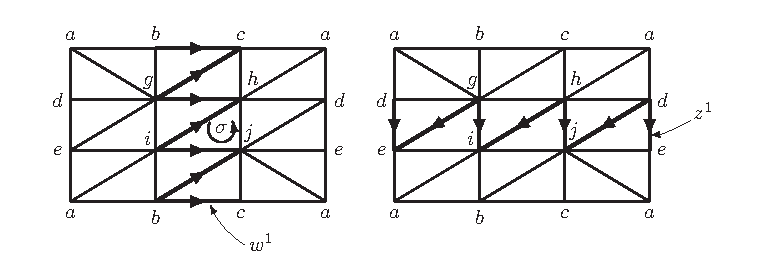
\includegraphics[width=.96\textwidth]{figures/8-8-1.pdf}
\caption*{图 8.8.1}
\end{figure}

\sourcepage{483--484}
定理的证明也说明为何应当如此。从 $w^1$ 出发，几何对偶映射 $\psi$ 将它映到图 8.8.2 中的闭链 $c_1$。该链承载于 $w^1$ 支承单形的对偶块中；要确认符号为 $c_1$ 而不是 $-c_1$，需要仔细检验。它与矩形侧边的胞腔 $B$ 所代表闭链同调。再通过代数对偶，$B$ 对应于在 $B$ 上取 $1$、在另一方向闭链 $A$ 上取 $0$ 的上闭链，$z^1$ 正是这样的上闭链。因此组合对偶把 $w^1$ 对应到 $z^1$，与 $\{z^1\smile w^1\}=\Lambda$ 以及两者的平方均为零相符。

\begin{figure}[htbp]\centering
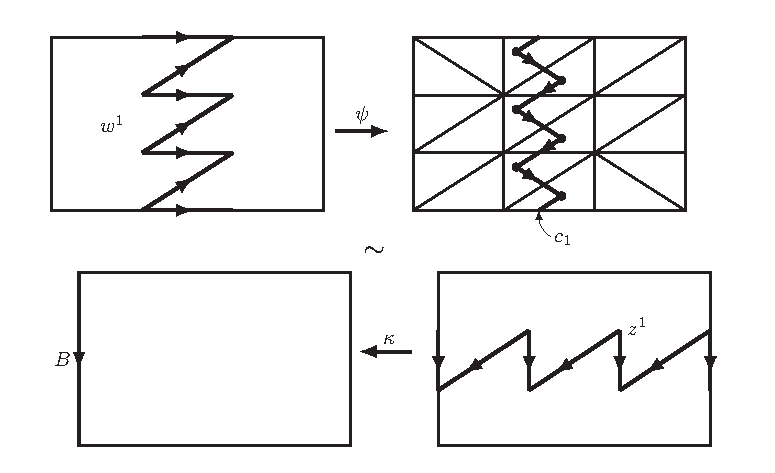
\includegraphics[width=.96\textwidth]{figures/8-8-2.pdf}
\caption*{图 8.8.2}
\end{figure}

现在研究实射影空间 $P^n$。它可三角剖分（引理 4.14.11），所以可用对偶定理。其胞腔链群在 $0\le k\le n$ 每维为 $\Z$，边缘为零或乘以 $2$，因此 $H^k(P^n;\Z/2)$ 在这些维数均为一维。还需计算杯积。以下用 $u^r$ 表示 $r$ 个 $u$ 的重复杯积。

\entry{定理}{8.8.5}若 $u$ 是 $H^1(P^n;\Z/2)$ 的非零元，则 $u^k$ 是 $H^k(P^n;\Z/2)$ 的非零元，$2\le k\le n$。因此
\[H^*(P^n;\Z/2)\cong(\Z/2)[u]/(u^{n+1}),\qquad\deg u=1.\]
即这是一个以一维元生成、在 $n+1$ 次截断的多项式代数。

\textbf{证明：}从 $n=2$ 开始归纳。此时 $H^1$ 一维，由定理 8.8.3，唯一非零元 $u$ 必满足 $u^2\ne0$。假定对 $n-1$ 成立。包含 $P^{n-1}\to P^n$ 在低于 $n$ 维诱导 $\Z/2$ 系数上同调同构，且保持杯积，所以 $u,u^2,\ldots,u^{n-1}$ 均非零。由定理 8.8.3，一维群 $H^1$ 和 $H^{n-1}$ 的生成元之积必须生成 $H^n$；它们唯一的非零元分别是 $u,u^{n-1}$，故 $u^n\ne0$。\hfill$\square$

\entry{推论}{8.8.6}$H^*(P^\infty;\Z/2)$ 是以一个一维元生成的多项式代数。

\textbf{证明：}包含 $P^n\to P^\infty$ 在不高于 $n$ 维诱导上同调同构，且保持杯积。\hfill$\square$

接着证明几个经典拓扑定理。

\entry{定义}{8.8.7}若映射满足 $f(-x)=-f(x)$，则称其\emph{保持对径点}。

\entry{定理}{8.8.8}若 $f:S^n\to S^m$ 连续且保持对径点，则 $n\le m$。

\sourcepage{485}
\textbf{证明：}记 $a_n=(1,0,\ldots,0)\in S^n$ 为基点，$F=\Z/2$。

第一步：设 $\pi_n:S^n\to P^n$ 是通常商映射。若 $\alpha$ 为从 $a_n$ 到 $-a_n$ 的任意道路，则 $\pi_n\alpha$ 代表 $H_1(P^n;F)$ 的非零元。

\begin{figure}[htbp]\centering
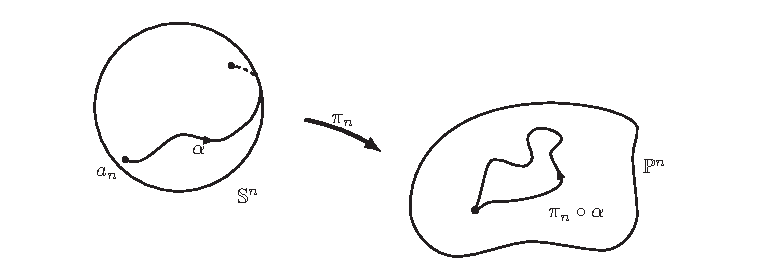
\includegraphics[width=.96\textwidth]{figures/8-8-3.pdf}
\caption*{图 8.8.3}
\end{figure}

先取标准道路 $\beta(t)=(\cos\pi t,\sin\pi t,0,\ldots,0)$。它把 $(I,\Bd I)$ 同胚到上半圆及其端点。$\pi_1$ 将端点粘合，映到 $(P^1,P^0)$。由 CW 复形的基本结果，相对生成元的像为一维胞腔的基本闭链，故 $\pi_n\beta$ 生成 $H_1(P^n;F)$。

一般地，$\alpha-\beta$ 是 $S^n$ 中的奇异闭链。若 $n>1$，$H_1(S^n)=0$，所以它是某二维链 $d$ 的边界。于是 $\pi_n\alpha-\pi_n\beta=\partial(\pi_{n\#}d)$，二者同调。若 $n=1$，商映射的度为 $2$，因此该差的像代表整数生成元的偶数倍，模 $2$ 后仍为零。第一步得证。

\sourcepage{486}
第二步：将 $f$ 与目标球面的旋转 $\rho$ 复合，使 $g=\rho f$ 把 $a_n$ 映到 $a_m$。它仍保持对径点，因而诱导 $h:P^n\to P^m$，满足 $h\pi_n=\pi_mg$。若 $\alpha$ 从 $a_n$ 通向 $-a_n$，则 $g\alpha$ 从 $a_m$ 通向 $-a_m$。由第一步，$h_*$ 把一维同调的非零元映到非零元。

第三步：由 Kronecker 同构的自然性，$h^*:H^1(P^m;F)\to H^1(P^n;F)$ 也非零。若 $u$ 为源的非零元，则 $h^*u$ 为目标的非零元。保持杯积给出
\[h^*(u^n)=(h^*u)^n\ne0.\]
故 $u^n\ne0$，从而 $m\ge n$。\hfill$\square$

\entry{定理}{8.8.9（Borsuk--Ulam 定理）}若 $h:S^n\to\R^n$ 连续，则存在 $x$ 使 $h(x)=h(-x)$。

\textbf{证明：}否则
\[f(x)=\frac{h(x)-h(-x)}{\|h(x)-h(-x)\|}\]
给出连续且保持对径点的 $S^n\to S^{n-1}$ 映射，与上一定理矛盾。\hfill$\square$

\entry{定理}{8.8.10（初等形式的火腿三明治定理）}平面中任意两个有界可测集合 $A_1,A_2$，可被同一直线按面积同时二等分。

\entry{注}{8.8.11}这个结论并不初等。即使两个集合都是三角区域，也可以试着寻找这样的直线。

\sourcepage{487}
\textbf{证明：}把平面视为 $\R^3$ 中的 $\R^2\times\{1\}$。对单位向量 $u\in S^2$，令 $P(u)$ 为过原点且垂直于 $u$ 的平面；$f_i(u)$ 为 $A_i$ 位于 $P(u)$ 的 $u$ 一侧的部分的测度。于是
\[f_i(u)+f_i(-u)=\operatorname{measure}(A_i).\]
映射 $u\mapsto(f_1(u),f_2(u))$ 连续。由 Borsuk--Ulam 定理，存在 $a$ 使 $f_i(a)=f_i(-a)$，从而均等于 $A_i$ 测度的一半。$P(a)$ 与原平面的交线就是所需直线。\hfill$\square$

\begin{figure}[htbp]\centering
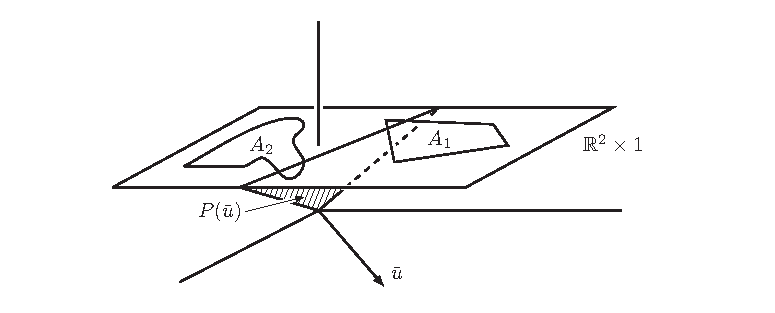
\includegraphics[width=.96\textwidth]{figures/8-8-4.pdf}
\caption*{图 8.8.4}
\end{figure}

证明可直接推广：$\R^n$ 中任意 $n$ 个有界可测集合，都可被同一 $(n-1)$ 维超平面同时二等分。名称来自三维情形：把三明治想成两片面包夹一片火腿，一刀即可同时把三片各自平分。

\sourcepage{488--489}
\subsection*{习题}
\begin{enumerate}
\item 设 $T$ 如例 8.8.4，$g:\operatorname{sd}T\to T$ 是恒等映射的单纯逼近。令 $\operatorname{sd}\gamma$ 为所有逆时针定向二维单形之和，验证 $g^\#w^1\frown\operatorname{sd}\gamma$ 为图 8.8.2 的 $c_1$。
\item \begin{enumerate}[label=(\alph*)]
\item 若 $\varphi:R\to R'$ 是有单位元交换环之间的同态，证明诱导的 $H^*(X;R)\to H^*(X;R')$ 为环同态。
\item 用系数同态 $\Z\to\Z/2$ 计算 $P^{2k},P^{2k+1},P^\infty$ 的整数上同调环。
\end{enumerate}
\item 证明任意时刻，地球表面都有一对对径点，其温度与气压分别相同。
\item 计算：(a) $S^3\times P^5$ 的 $\Z$ 及 $\Z/2$ 系数上同调环；(b) $P^2\times P^3$ 的 $\Z/2$ 系数上同调环。
\item 假设 $\mathbb{CP}^n$ 可三角剖分（事实上确实可以）。
\begin{enumerate}[label=(\alph*)]
\item 计算 $H^*(\mathbb{CP}^n)$ 和 $H^*(\mathbb{CP}^\infty)$。
\item 对 $f:\mathbb{CP}^n\to\mathbb{CP}^n$，证明其度为某整数 $a$ 的 $n$ 次方。
\item 证明 $\mathbb{CP}^{2n}$ 的每个自映射都有不动点。
\item 证明不存在度为 $-1$ 的 $\mathbb{CP}^{2n}$ 自映射。
\item 若 $\mathbb{CP}^{2n+1}$ 的自映射无不动点，其度是多少？
\end{enumerate}
\item 〔*〕从两个 $\mathbb{CP}^2$ 各删去一个小开四维球，再沿边界三维球面粘合得到流形 $M$。讨论其上同调环，并与 $S^2\times S^2$ 比较。
\item 设 $X$ 为连通、可三角剖分的同调七维流形，满足
\[H^7(X)\cong\Z,\quad H^6(X)\cong\Z,\quad H^5(X)\cong\Z/2,\quad
H^4(X)\cong\Z\oplus\Z/3.\]
尽可能确定其他上同调群及环结构。
\item 设 $X$ 是紧致可定向、可三角剖分的同调 $(4n+2)$ 维流形。证明不可能有 $H^{2n+1}(X)\cong\Z$。
\item 令 $X_0=S^2$，$X_n$ 为 $n$ 个环面的连通和，$Y_n$ 为 $n$ 个射影平面的连通和。考察 $f_*$ 在 $\Z/2$ 系数二维同调上非零这一条件。
\begin{enumerate}[label=(\alph*)]
\item 证明不存在满足条件的 $Y_{2n}\to X_n$。〔提示：自由群之间的同态，若源秩大于目标秩，则核有正秩且为直和分量。选择 $H^1(X_n)$ 的基使 $f^*(\beta_1)=0$，再转为模 $2$ 系数，应用定理 8.8.3 的证明。〕
\item 证明存在满足条件的 $Y_{2n+1}\to X_n$。〔提示：先证 $Y_3\approx T\mathbin{\#}P^2$。〕
\item 证明存在满足条件的 $Y_m\to X_n$，当且仅当 $m\ge2n+1$。
\end{enumerate}
\item 举出不保持对径点的连续映射 $S^2\to S^2$。每个维数都有这样的例子吗？
\item 表述四维空间中的火腿三明治定理，并尝试证明。
\end{enumerate}

\section{*应用：透镜空间的同伦分类}
\sourcepage{489--490}
本节假定读者熟悉透镜空间（第 4.14 节）。上同调的杯积环结构通过 Poincaré 对偶同构，诱导同调上的环结构，称为\emph{同调交环}。在上同调被发现以前，这个环就已经为人所知。粗略地说，两个同调类的交积由代表它们的闭链的几何交定义。这样定义运算并推导性质，需要相当多工作。虽然运算是拓扑不变量，但一般连续映射即使在同维流形之间也不保持它。因此，把交积推广到任意多面体的努力未能成功，也并不令人意外。

今天我们把上同调环视为自然对象，把流形同调交环的存在看成由 Poincaré 对偶带来的有利现象。这里不详细研究交环，只证明一个把交积解释为闭链几何交的引理，以便计算透镜空间的上同调环。

\entry{记号}{8.9.1}本节 $X$ 始终为紧致连通、可三角剖分的 $n$ 维流形。若可定向，$\Gamma$ 为定向类，$R$ 为任意有单位元交换环；若不可定向，令 $\Gamma=\Gamma_{(2)}$，$R=\Z/2$。

\entry{定义}{8.9.2}对 $\alpha_p\in H_p(X;R)$、$\beta_q\in H_q(X;R)$，取唯一的类满足
\[\alpha^{n-p}\frown\Gamma=\alpha_p,\qquad\beta^{n-q}\frown\Gamma=\beta_q,\]
定义\emph{交积}
\[\alpha_p\cdot\beta_q=(\alpha^{n-p}\smile\beta^{n-q})\frown\Gamma.\]
可定向情形下结果的符号依赖于定向类。积的维数为 $p+q-n$，这与 $\R^n$ 中一般位置的 $p$ 维平面与 $q$ 维平面的交的维数相同，因而暗示它与几何交有关。

\entry{引理}{8.9.3}采用上述记号，设 $p+q=n$。类 $\alpha_p$ 由承载于对偶 $p$ 维骨架的重分后闭链 $c_p$ 代表，$\beta_q$ 由原复形的闭链 $d_q$ 代表。假设二者的承载集只交于一个 $q$ 维单形 $\sigma$ 的重心。若 $d_q$ 在 $\sigma$ 上的系数为 $\pm a$，$c_p$ 在对偶块 $D(\sigma)$ 上的系数为 $\pm b$，则其交积差一个符号由零维链 $ab\widehat\sigma$ 代表。

\sourcepage{491}
\textbf{证明：}取 $\alpha^q,\beta^p$ 为对应上同调类。由定义及帽积公式，
\[\alpha_p\cdot\beta_q=(\alpha^q\smile\beta^p)\frown\Gamma
=\alpha^q\frown\beta_q.\]
增广诱导 $H_0(X;R)\cong R$，故只需证明
\[\langle\alpha^q,\beta_q\rangle=\epsilon_*(\alpha_p\cdot\beta_q)=\pm ab.\]
取代表 $\Gamma$ 的顶维闭链 $\gamma$，并使用上一节构造的同构
\[\psi:C^q(X)\to\mathcal D_p(X),\qquad
j\psi(c^q)=g^\#c^q\frown\operatorname{sd}\gamma.\]
对有向 $q$ 维单形 $\sigma_i$，记对应对偶块的基本闭链 $z_i=\psi(\sigma_i^*)$。写
\[c_p=\sum b_jz_j,\qquad c^q=\sum b_j\sigma_j^*.\]
因 $\partial\psi=\pm\psi\delta$，$c^q$ 是上闭链；又因 $\psi$ 诱导 $\frown\Gamma$，它代表 $\alpha^q$。再写 $d_q=\sum a_i\sigma_i$。$D(\sigma_j)$ 与 $q$ 维单形 $\sigma_i$ 只有 $i=j$ 时相交，交点为重心。由承载集只交一点，只有对应 $\sigma$ 的指标能同时有 $a_i,b_i\ne0$。因此
\[\langle\alpha^q,\beta_q\rangle=\langle c^q,d_q\rangle
=\sum b_ja_i\langle\sigma_j^*,\sigma_i\rangle=\sum b_ia_i=\pm ba.\]
\hfill$\square$

为应用于透镜空间，还需要 Bockstein 运算；同调版本已在定义 3.3.10 引入。

\sourcepage{492--493}
\entry{定义}{8.9.4}设 $C$ 为自由链复形。系数短正合列 $0\to G\to G'\to G''\to0$ 给出链群及上链群的短正合列
\[
0\to C_p\otimes G\to C_p\otimes G'\to C_p\otimes G''\to0,
\]
\[
0\to\operatorname{Hom}(C_p,G)\to\operatorname{Hom}(C_p,G')\to\operatorname{Hom}(C_p,G'')\to0.
\]
由折线引理得到自然连接同态
\[\beta_*:H_p(C;G'')\to H_{p-1}(C;G),\qquad
\beta^*:H^p(C;G'')\to H^{p+1}(C;G),\]
称为该系数序列对应的\emph{Bockstein 同态}。

\entry{引理}{8.9.5}若 $X$ 可定向，则 Bockstein 同态与 Poincaré 对偶同构相差一个符号地交换。

\textbf{证明：}用定理 8.5.2 的 $\varphi:C^k(X)\to\mathcal D_{n-k}(X)$，对系数短正合列张量，得到两行短正合列之间的交换图，其竖直映射为 $\varphi\otimes i$。由于 $\partial\varphi=\varphi\delta$，连接同态也交换，所以
\[
\begin{array}{ccc}
H^k(X;G'')&\xrightarrow{\beta^*}&H^{k+1}(X;G)\\
\downarrow\cong&&\downarrow\cong\\
H_{n-k}(X;G'')&\xrightarrow{\beta_*}&H_{n-k-1}(X;G).
\end{array}
\]
这里利用了自然上链同构 $C^i(X)\otimes G\cong\operatorname{Hom}(C_i(X),G)$，以及折线构造的自然性。因此可以用这些复形计算对应 Bockstein。$\varphi$ 诱导的同构与帽积同构仅差一个符号，所以结论成立。\hfill$\square$

回顾 $X=L(n,k)$ 是紧致连通、可定向、可三角剖分的三维流形，其中 $n,k$ 为互素正整数。它有每维一个胞腔的 CW 结构，胞腔边缘为零或乘以 $n$。故对 $i=1,2,3$，
\[H_i(X;\Z/n)\cong\Z/n\cong H^i(X;\Z/n).\]

\entry{定理}{8.9.6}取 $H^3(X)$ 的生成元 $\Lambda$，其在模 $n$ 系数下的像为 $\Lambda_{(n)}$。令 $\beta^*:H^1(X;\Z/n)\to H^2(X;\Z/n)$ 对应系数列
\[0\to\Z/n\xrightarrow{\varphi_n}\Z/n^2\to\Z/n\to0,\]
其中 $\varphi_n$ 为乘以 $n$。则存在 $H^1(X;\Z/n)$ 的生成元 $u$，使
\[u\smile\beta^*(u)=\pm[k]^{-1}\Lambda_{(n)},\]
这里 $[k]^{-1}$ 是环 $\Z/n$ 中 $[k]$ 的逆元。

\textbf{证明：}由 Bockstein 与对偶相差符号地交换，只需在同调中找生成元 $w\in H_2(X;\Z/n)$，使
\[w\cdot\beta_*(w)=\pm[k]^{-1}(\Lambda_{(n)}\frown\Gamma).\]
右侧括号内是 $H_0(X;\Z/n)$ 的生成元，等于顶点 $v_0$ 取系数 $[1]$ 所代表的类。

\sourcepage{494}
令 $v,e,c$ 分别为零、一、二维胞腔的基本链，如图 8.9.1。第 4.14 节证明了 $\partial c=ne$。模 $n$ 后它成为闭链，令 $w=\{c\}$，这生成二维同调。

\begin{figure}[htbp]\centering
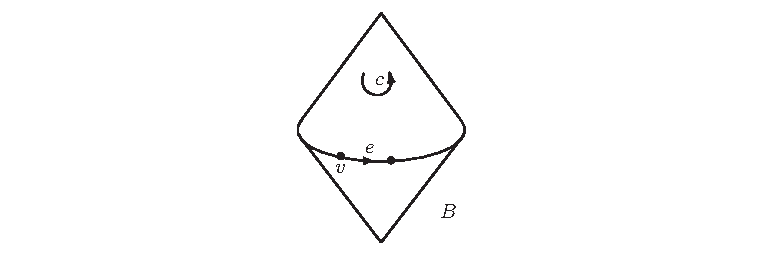
\includegraphics[width=.88\textwidth]{figures/8-9-1.pdf}
\caption*{图 8.9.1}
\end{figure}

用胞腔复形和折线引理计算 $\beta_*w$：先将 $c$ 提升为模 $n^2$ 的链，取边界 $ne$，再除以 $n$，得到 $\beta_*w=\{e\}$。

要算交积 $\{c\}\cdot\{e\}$，不能直接用前引理，因为二者承载集的交不止一点。先以同调链替代。图 8.9.2 中的 $d$ 与 $c$ 同调，因为实心上半部分适当定向后的边界为 $c-d$。再取从多面体顶部到底部的闭链 $z$（图 8.9.3）。它在透镜空间中与 $-ke$ 同调：顶点 $v$ 与其旋转像 $r_\theta(v)$ 之间有 $k$ 条一维胞腔，$\theta=2\pi k/n$；图中阴影二维链在多面体内的边界为 $ke+z+s_1+s_2$，两条斜链在商空间粘合后抵消，所以边界为 $ke+z$。

\begin{figure}[htbp]\centering
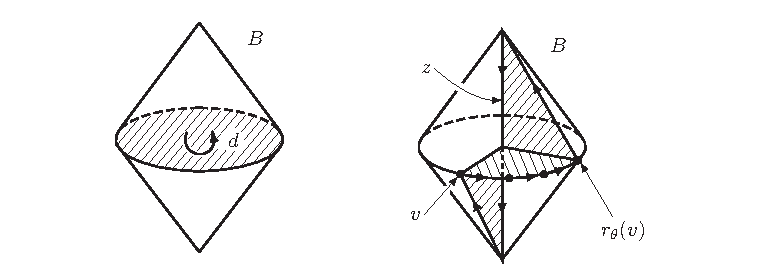
\includegraphics[width=.96\textwidth]{figures/8-9-2-3.pdf}
\caption*{图 8.9.2（左）与图 8.9.3（右）}
\end{figure}

\sourcepage{495}
$d,z$ 的承载集只交一点。严格地说，还需三角剖分，并将 $z$ 推到对偶一维骨架上，保持只有一个交点，这并不困难。由引理 8.9.3，$\{d\}\cdot\{z\}$ 为指定零维生成元的 $\pm1$ 倍。代入 $\{d\}=w$、$\{z\}=-k\beta_*w$，得到所需结论。\hfill$\square$

\entry{定理}{8.9.7}若 $L(n,k)$ 与 $L(n,\ell)$ 同伦等价，则必存在整数 $a$，使
\[k\equiv\pm a^2\ell\pmod n.\]

\textbf{证明：}设 $f:X\to Y$ 为同伦等价，取前一定理的生成元 $u,v$ 及顶维类 $\Lambda,\Lambda'$。写 $f^*v=au$。由 Bockstein 自然性及杯积自然性，
\begin{align*}
\pm[\ell]^{-1}f^*(\Lambda'_{(n)})
&=f^*(v\smile\beta^*v)
=f^*v\smile\beta^*(f^*v)\\
&=a^2(u\smile\beta^*u)=\pm a^2[k]^{-1}\Lambda_{(n)}.
\end{align*}
同伦等价使 $f^*\Lambda'=\pm\Lambda$，模 $n$ 后也如此，因此 $[\ell]^{-1}=\pm a^2[k]^{-1}$，即所需同余式。\hfill$\square$

\sourcepage{496}
此条件实际上既必要又充分；充分性由 J. H. C. Whitehead 证明。因此透镜空间是少数同胚分类与同伦分类都已解决的空间族（定理 4.14.15、注 4.14.16）。

Hurewicz 曾猜想：同伦等价的两个紧致流形应该同胚。二维时确实如此，但透镜空间给出三维反例。$L(7,1)$ 与 $L(7,2)$ 同伦等价，因为 $2\equiv3^2\pmod7$；但并不同胚，因为 $2\not\equiv\pm1$，且 $2\cdot1\not\equiv\pm1\pmod7$。

习题 3 表明，单凭 $H^*(L(n,k);\Z/n)$ 的环结构不足以作同伦分类，还需要 Bockstein。这是\emph{上同调运算}的一个例子。

\entry{定义}{8.9.8}类型为 $(p,q;G,G')$ 的上同调运算，是对每个拓扑偶定义的集合映射
\[\theta:H^p(X,A;G)\to H^q(X,A;G'),\]
并且相对于连续映射诱导的同态自然。\translatornote{原文目标系数有排印错误，这里按所声明的类型写作 $G'$。}

上同调运算赋予空间上同调远比环更丰富的结构。与透镜空间的例子一样，这些运算常能提供有价值的信息。

\sourcepage{496--497}
\subsection*{习题}
\begin{enumerate}
\item 若 $f:L(n,k)\to L(n,\ell)$ 的度为 $d$，证明存在整数 $a$，使 $kd\equiv\pm a^2\ell\pmod n$。
\item 利用本节结论、定理 4.14.15 及注 4.14.16，分别对 $L(7,k)$（$1\le k\le6$）和 $L(10,k)$（$k$ 与 $10$ 互素）作同胚分类及同伦分类。
\item 设 $X=L(n,k)$。
\begin{enumerate}[label=(\alph*)]
\item 若 $u_i$ 生成 $H^i(X;\Z/n)$，$i=1,2$，证明 $u_1\smile u_2$ 生成 $H^3(X;\Z/n)$。〔提示：先证明 $\beta^*:H^1\to H^2$ 是同构，从而存在一组这样的生成元。〕
\item 证明 $u_1\smile u_1$ 为零或阶为 $2$。\translatornote{原文此处写作 $u_1\smile u_2$，与 (a) 矛盾；按反交换律所适用的平方应为 $u_1\smile u_1$。}
\end{enumerate}
\item 对两个不同的自由链复形，各给出一个 Bockstein 同态的例子。
\end{enumerate}

\section{Lefschetz 对偶}
\sourcepage{497--498}
正如预期，Poincaré 对偶可推广到相对同调流形，这一推广归功于 Lefschetz。在流形情形，它具有特别漂亮的形式。

先回顾：若 $X$ 中任意顶点全在 $A$ 的单形都属于 $A$，就称 $A$ 为\emph{满子复形}。一般子复形不一定满，但重心重分后总成为满子复形。事实上，若重分单形的顶点均在 $\operatorname{sd}A$ 中，特别是最大顶点 $\widehat\sigma_1$ 在其中，则 $\Int\sigma_1$ 与 $|A|$ 相交，故 $\sigma_1\in A$，整个重分单形也在 $|A|$ 中。

\entry{引理}{8.10.1}设 $A$ 为有限复形 $X$ 的满子复形，$C$ 由所有与 $|A|$ 不交的单形组成。则 $|A|$ 是 $|X|\setminus|C|$ 的形变收缩核，$|C|$ 是 $|X|\setminus|A|$ 的形变收缩核。

\textbf{证明：}每个顶点属于 $A$ 或 $C$。$C$ 也是满子复形：顶点都在 $C$ 的单形不可能与 $|A|$ 相交。反过来，$A$ 也恰由所有与 $|C|$ 不交的单形组成，因为这样的单形顶点都在 $A$ 中。由对称性只证第一个结论。

若 $\sigma$ 既不属于 $A$ 也不属于 $C$，则 $\sigma=s*t$，其中 $s$ 由属于 $A$ 的顶点张成，$t$ 由属于 $C$ 的顶点张成。每个 $x\in\sigma\setminus(s\cup t)$ 都在连接两部分的唯一线段内部。令 $f_\sigma(x)$ 为该线段在 $s$ 一侧的端点，并在 $s$ 上取恒等。若 $s=v_0\cdots v_p$、$t=v_{p+1}\cdots v_r$，则
\[x=\sum_{i=0}^r\alpha_iv_i\quad\Longrightarrow\quad
f_\sigma(x)=\sum_{i=0}^p\frac{\alpha_i}{\lambda}v_i,\qquad\lambda=\sum_{i=0}^p\alpha_i>0.\]
所以 $f_\sigma$ 连续。这些映射在公共部分相容，且在 $|A|$ 上为恒等，因此拼成收缩 $f:|X|\setminus|C|\to|A|$。令 $F(x,t)=(1-t)x+tf(x)$，即为所需形变收缩。\hfill$\square$

引理在无限复形情形也成立，但连续性需要额外注意；有限情形没有这个问题。

\entry{定义}{8.10.2}设 $(X,A)$ 为紧致、已三角剖分的相对同调 $n$ 维流形。若能给所有不属于 $A$ 的顶维单形定向，使其和 $\gamma$ 为相对闭链，则称该偶\emph{可定向}，称 $\gamma$ 为\emph{定向闭链}。

\entry{定理}{8.10.3（Lefschetz 对偶）}若 $(X,A)$ 紧致、已三角剖分，且是可定向的相对同调 $n$ 维流形，则对任意 $G$，
\[H^k(X,A;G)\cong H_{n-k}(|X|\setminus|A|;G),\qquad
H_k(X,A;G)\cong H^{n-k}(|X|\setminus|A|;G).\]
若不可定向，取 $G=\Z/2$ 时仍成立。

\entry{注}{8.10.4}补空间的群应理解为奇异群，因为它不是原复形子复形的多面体（它实际上可三角剖分，但还未证明）。

\textbf{证明：}令 $X^*$ 为 $\operatorname{sd}X$ 中所有与 $|A|$ 不交的单形组成的子复形。$\operatorname{sd}A$ 满，故由引理 $|X^*|$ 是补空间的形变收缩核，可用它代替补空间。

\sourcepage{499}
断言：$|X^*|$ 等于所有不属于 $A$ 的单形所对应对偶块之并。若重分单形对应面链 $\sigma_1\succ\cdots\succ\sigma_k$，其内部属于 $D(\sigma_k)$。它与 $|A|$ 不交，当且仅当 $\sigma_k\notin A$：一个方向看最小顶点即可；反方向，若最小单形不在 $A$ 中，所有包含它的较大单形也不在 $A$ 中，故各重心均不在 $A$ 中，整个重分单形不与 $|A|$ 相交。

\begin{figure}[htbp]\centering
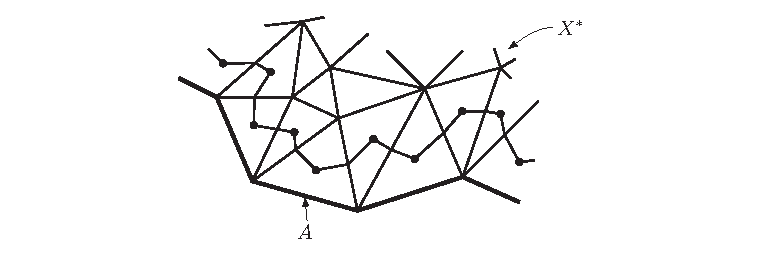
\includegraphics[width=.90\textwidth]{figures/8-10-1.pdf}
\caption*{图 8.10.1}
\end{figure}

这些块的重心位于 $X\setminus A$，局部同调满足流形条件，所以每个闭块模边界是维数 $n-\dim\sigma$ 的同调胞腔。它们组成对偶链复形 $\mathcal D(X^*)$，其包含到 $C(X^*)$ 的映射诱导任意系数的同调、上同调同构，理由同定理 8.4.8。

可定向情形，$C^k(X,A)$ 是在 $A$ 的单形上为零的上链群，其基由所有 $\sigma\notin A$ 的 $\sigma^*$ 构成。第一种 Poincaré 对偶证明原样给出
\[\varphi:C^k(X,A)\xrightarrow{\cong}\mathcal D_{n-k}(X^*),\qquad\varphi\delta=\partial\varphi.\]
于是得到第一个对偶同构。

\sourcepage{500}
有限自由链群的自然双对偶同构把 $\operatorname{Hom}(C^k(X,A),\Z)$ 与 $C_k(X,A)$ 等同。再将 $\varphi$ 对偶化，就得到相对同调与对偶复形上同调的同构，进而得到第二个对偶同构。任意系数以及不可定向时的模 $2$ 情形，与 Poincaré 对偶证明相同。\hfill$\square$

\entry{推论}{8.10.5}若补空间连通，则任意两个不属于 $A$ 的顶维单形之间，都有相邻单形交于不属于 $A$ 的余维一面的有限顶维单形序列。

\textbf{证明：}以这种序列定义等价关系。每个等价类之和均为模 $2$ 相对闭链，而
\[H_n(X,A;\Z/2)\cong H^0(|X|\setminus|A|;\Z/2)\cong\Z/2,\]
所以只有一个等价类。\hfill$\square$

\entry{推论}{8.10.6}若补空间连通，则可定向时 $H_n(X,A)\cong\Z$，不可定向时 $H_n(X,A)=0$。

证明同推论 8.5.4。

\sourcepage{501}
\entry{推论}{8.10.7}令 $X_i$ 为补空间各连通分支的闭包，$A_i=X_i\cap A$。则 $(X,A)$ 可定向，当且仅当每个 $H_n(X_i,A_i)\cong\Z$。

\entry{注}{8.10.8}因此相对可定向性与三角剖分无关。

\entry{定义}{8.10.9}设 $(X,A)$ 为紧致、可三角剖分的相对同调 $n$ 维流形。采用上一推论的记号。可定向时，选取每个 $H_n(X_i,A_i)$ 的生成元 $\Gamma^{(i)}$，称为该偶的定向类；它们的和通过包含诱导同构
\[\bigoplus_i H_n(X_i,A_i)\cong H_n(X,A)\]
的像称为 $(X,A)$ 的\emph{定向类}，记为 $\Gamma$。不要求可定向时，取各模 $2$ 顶维相对同调的唯一非零元，其和记为 $\Gamma_{(2)}$。若给定剖分，分别由适当定向的全部不属于 $A$ 的顶维单形之和，或这些单形均取系数 $[1]$ 的和代表。

自然会问：帽积形式的第二种证明能否直接推广？一般不能。选恒等映射的单纯逼近 $g:(\operatorname{sd}X,\operatorname{sd}A)\to(X,A)$，以及定向相对闭链 $\gamma$。前面的论证仍表明复合
\[C^k(X,A)\xrightarrow{g^\#}C^k(\operatorname{sd}X,\operatorname{sd}A)
\xrightarrow{\frown\operatorname{sd}\gamma}C_{n-k}(\operatorname{sd}X)\]
同构地映到对偶链子群 $\mathcal D_{n-k}(X^*)$，并与 $\varphi$ 仅差一个符号。

\sourcepage{502}
困难发生在通过同调时：帽积的目标是 $H_{n-k}(X)$，而不是所需的 $H_{n-k}(X\setminus A)$。因此一般不能直接把 Lefschetz 对偶同构写成与 $\Gamma$ 的帽积，只能得到如下关系。

\entry{定理}{8.10.10}令 $j:X\setminus A\to X$ 为包含，$\varphi_*$ 为 Lefschetz 对偶同构。则对可定向的紧致可三角剖分相对同调流形，
\[\frown\Gamma=\pm j_*\varphi_*:H^k(X,A;G)\to H_{n-k}(X;G),\]
符号只依赖 $k,n$。不可定向情形以 $\Gamma_{(2)}$ 和 $\Z/2$ 代替，结论同样成立。

\textbf{证明：}选取剖分，比较 $\varphi$ 与上述重分后帽积复合。第 8.7 节的证明说明二者相差维数相关的符号。再将对偶链包含到 $X^*$ 的单纯链，映到奇异链，并由包含映入补空间及 $X$；单纯到奇异的链映射保持帽积，其余包含映射显然交换。通过同调即得结论。\hfill$\square$

对带边界流形，对偶同构确实可以由帽积直接给出。

\sourcepage{503--504}
\entry{定义}{8.10.11}若有同胚 $h:\Bd M\times[0,1)\to U$，其中 $U$ 是 $M$ 中开集，且 $h(x,0)=x$，则称边界在 $M$ 中有\emph{乘积邻域}。这样的邻域实际上总存在，但证明并不简单（见 [Bro62]）。

\entry{定理}{8.10.12（Poincaré--Lefschetz 对偶）}设 $M$ 是紧致、可三角剖分的带边界 $n$ 维流形，边界有乘积邻域。若 $(M,\Bd M)$ 可定向，取定向类 $\Gamma$，则对任意 $G$，
\[H^k(M,\Bd M;G)\xrightarrow{\frown\Gamma}H_{n-k}(M;G),\]
\[H^k(M;G)\xrightarrow{\frown\Gamma}H_{n-k}(M,\Bd M;G)\]
都是同构。不可定向时，取 $\Z/2$ 系数与 $\Gamma_{(2)}$ 也成立。

\begin{figure}[htbp]\centering
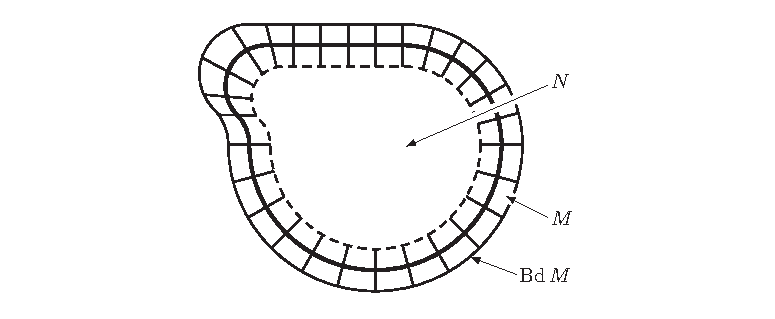
\includegraphics[width=.90\textwidth]{figures/8-10-2.pdf}
\caption*{图 8.10.2}
\end{figure}

\textbf{证明：}取边界乘积邻域 $h$，令
\[N=M\setminus h(\Bd M\times[0,1/2)).\]
将乘积参数向 $1/2$ 推动，表明 $N$ 同时是 $M$ 与 $M\setminus\Bd M$ 的形变收缩核。因此内部到 $M$ 的包含为同伦等价，诱导同调同构。第一个帽积同构随即由定理 8.10.10 得到。

证明第二个。三角剖分边界是 $(n-1)$ 维单形之并，每个边界余维一面恰为一个顶维单形的面：至少有一个，因为 $M$ 由顶维单形组成；不能多于一个，因为边界点的局部同调为零，而引理 8.3.2 把该局部群与链环的约化零维同调等同。

若 $\gamma$ 是相对定向闭链，则 $\partial\gamma$ 在每个边界顶维单形上系数均为 $\pm1$，且为闭链，所以是边界的定向闭链。故 $\partial_*\Gamma$ 是 $\Bd M$ 的定向类。比较偶的上同调、同调长正合列中的五项，对应竖直映射依次为
\[\frown\partial_*\Gamma,\quad\frown\Gamma,\quad\frown\Gamma,\quad
\frown\partial_*\Gamma,\quad\frown\Gamma.\]
源的五项依次为 $H^{k-1}(\Bd M),H^k(M,\Bd M),H^k(M),H^k(\Bd M),H^{k+1}(M,\Bd M)$；目标为相应的 $H_{n-k}(\Bd M),H_{n-k}(M),H_{n-k}(M,\Bd M),H_{n-k-1}(\Bd M),H_{n-k-1}(M)$。图相差符号地交换。第一、四项由 Poincaré 对偶为同构，第二、五项由刚证明的第一个同构为同构，因此五引理给出中间项同构。模 $2$ 时证明相同。\hfill$\square$

给定紧致流形，什么时候它是某个高一维紧致流形的边界？研究这一问题的完整理论称为\emph{配边理论}。下面只证明一个初等结果。

\sourcepage{505--506}
\entry{定理}{8.10.13}设 $M$ 是紧致、可三角剖分的带边界 $(2m+1)$ 维流形，边界非空且有乘积邻域。则 $H_m(\Bd M;\Z/2)$ 的维数为偶数。

\textbf{证明：}第一步：对只在有限范围非零的向量空间正合列 $\cdots\to A_{k-1}\xrightarrow{\varphi_{k-1}}A_k\xrightarrow{\varphi_k}A_{k+1}\to\cdots$，有
\[
\operatorname{rank}\varphi_k=\dim A_k-\dim A_{k-1}+\dim A_{k-2}-\cdots,
\]
\[
\operatorname{rank}\varphi_{k-1}=\dim A_k-\dim A_{k+1}+\dim A_{k+2}-\cdots.
\]
因为正合性给出 $\dim A_i=\operatorname{rank}\varphi_{i-1}+\operatorname{rank}\varphi_i$，交错求和即可。

第二步：取模 $2$ 上同调长正合列中的映射
\[H^k(M)\xrightarrow{\mu_k}H^k(\Bd M)\xrightarrow{\nu_k}H^{k+1}(M,\Bd M).\]
记三类群的维数分别为 $\beta_k,\gamma_k,\alpha_{k+1}$。第一步给出
\[\operatorname{rank}\nu_k=\sum_{i\ge0}(-1)^i(\gamma_{k-i}-\beta_{k-i}+\alpha_{k-i}),\]
\[\operatorname{rank}\mu_k=\sum_{i\ge0}(-1)^i(\gamma_{k+i}-\alpha_{k+i+1}+\beta_{k+i+1}).\]
令 $n=\dim M$。Lefschetz 对偶、边界上的 Poincaré 对偶以及域系数代数对偶给出
\[\alpha_j=\beta_{n-j},\qquad\gamma_j=\gamma_{n-j-1}.\]
代入比较两式，得 $\operatorname{rank}\mu_k=\operatorname{rank}\nu_{n-k-1}$。当 $n=2m+1$ 时，$\operatorname{rank}\mu_m=\operatorname{rank}\nu_m$，所以
\[\dim H_m(\Bd M;\Z/2)=\gamma_m=2\operatorname{rank}\nu_m,\]
为偶数。\hfill$\square$

\entry{推论}{8.10.14}$P^{2m}$ 不是紧致、可三角剖分的 $(2m+1)$ 维流形的边界。

\subsection*{习题}
\begin{enumerate}
\item 设 $(X,A)$ 是紧致、可三角剖分的相对同调 $n$ 维流形，补空间连通。证明可定向时
\[H_n(X,A;G)\cong G\cong H^n(X,A;G),\]
不可定向时
\[H_n(X,A;G)\cong\ker\varphi_2,\qquad H^n(X,A;G)\cong G/2G,\]
其中 $\varphi_2$ 为乘以 $2$。
\item 设 $M$ 是紧致可定向、可三角剖分的带边界 $n$ 维流形，边界为两个 $(n-1)$ 维流形 $V_0,V_1$ 的不交并，且有乘积邻域。取相对定向类 $\Gamma$，证明
\[\frown\Gamma:H^k(M,V_0)\longrightarrow H_{n-k}(M,V_1)\]
为同构。〔提示：考虑三元组 $(M,\Bd M,V_1)$ 的正合列。〕
\item 利用复射影空间可三角剖分，证明 $\mathbb{CP}^{2m}$ 不是任何流形的边界。
\item 哪些紧致二维流形能够成为边界？
\item 设 $M$ 为紧致可定向、可三角剖分的带边界 $n$ 维流形。证明杯积给出对偶配对
\[\frac{H^k(M,\Bd M)}{T^k(M,\Bd M)}\otimes
\frac{H^{n-k}(M)}{T^{n-k}(M)}\to H^n(M,\Bd M),\]
其中 $T^i$ 表示相应上同调群的挠子群。
\item 设 $M$ 是从环面删去两个开圆盘所得的空间（图 8.10.3）。
\begin{enumerate}[label=(\alph*)]
\item 计算 $H^1(M)$、$H^1(M,\Bd M)$，画出生成上闭链。
\item 验证上一题的对偶配对。
\item 证明两个相对一维上同调因子的杯积
\[\frac{H^1(M,\Bd M)}{T^1(M,\Bd M)}\otimes
\frac{H^1(M,\Bd M)}{T^1(M,\Bd M)}\to H^2(M,\Bd M)\]
并不构成对偶配对。
\end{enumerate}
\begin{figure}[htbp]\centering
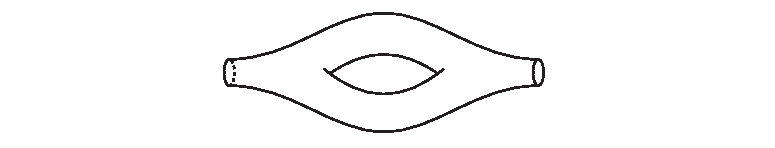
\includegraphics[width=.90\textwidth]{figures/8-10-3.pdf}
\caption*{图 8.10.3}
\end{figure}
\item 设 $X$ 为紧致、可三角剖分的同调 $n$ 维流形，$B\subset A$ 均为同一剖分的子复形多面体。可定向时 $G$ 任意，否则取 $G=\Z/2$。证明
\[H^k(A,B;G)\cong H_{n-k}(X\setminus B,X\setminus A;G),\]
\[H_k(A,B;G)\cong H^{n-k}(X\setminus B,X\setminus A;G).\]
〔提示：选择剖分使 $A,B$ 均为满子复形的多面体。对满子复形 $C$，记 $X_C$ 为重分后与 $C$ 不交的全部单形组成的复形。比较上链短正合列
\[0\to C^k(X,A)\to C^k(X,B)\to C^k(A,B)\to0\]
与对偶链短正合列
\[0\to\mathcal D_{n-k}(X_A)\to\mathcal D_{n-k}(X_B)
\to\mathcal D_{n-k}(X_B,X_A)\to0,\]
以及它们的对偶。〕
\item 〔*〕将 Lefschetz 对偶推广到非紧情形。
\item 设 $(X,A)$ 为非紧的已三角剖分相对同调 $n$ 维流形，且补空间连通。证明它是相对伪 $n$ 维流形。
\item 给出两个二维的紧致可三角剖分相对同调流形例子，并分别指定定向类。
\end{enumerate}

\section{Alexander 对偶}
\sourcepage{508--509}
Alexander 对偶几乎与 Poincaré 对偶同样古老，比 Lefschetz 对偶还早若干年。其原始形式描述 $n$ 维球面子复形的 Betti 数、挠系数与补空间对应不变量之间的关系。现代以上同调表述，并用 Lefschetz 对偶证明。

\entry{定理}{8.11.1}设 $A$ 是 $S^n$ 的非空真子集，且偶 $(S^n,A)$ 可三角剖分，则
\[\widetilde H^k(A)\cong\widetilde H_{n-k-1}(S^n\setminus A).\]

\textbf{证明：}排除平凡情形，假设 $n>0$，并三角剖分此偶。

第一步：设 $k\ne n,n-1$。考虑正合列
\[\widetilde H^k(S^n)\to\widetilde H^k(A)\xrightarrow{\delta^*}H^{k+1}(S^n,A)
\to\widetilde H^{k+1}(S^n).\]
两端为零，故中间连接映射为同构。由 Lefschetz 对偶，
\[H^{k+1}(S^n,A)\cong H_{n-k-1}(S^n\setminus A)
=\widetilde H_{n-k-1}(S^n\setminus A),\]
得到所需结论。

第二步：设 $k=n-1$。此时正合列给出
\[0\to\widetilde H^{n-1}(A)\xrightarrow{\delta^*}H^n(S^n,A)
\xrightarrow{j^*}H^n(S^n),\]
所以 $\widetilde H^{n-1}(A)\cong\ker j^*$。取球面的定向类 $\Gamma$，并记补空间包含为 $k:S^n\setminus A\to S^n$。Poincaré 对偶、Lefschetz 对偶以及帽积自然性给出相差符号地交换的图：上行为 $j^*$，下行为
\[k_*:H_0(S^n\setminus A)\to H_0(S^n),\]
竖直同构分别为 Lefschetz 对偶和 $\frown\Gamma$。因此 $\ker j^*\cong\ker k_*$。由正合列
\[0\to\widetilde H_0(S^n\setminus A)\to H_0(S^n\setminus A)
\xrightarrow{k_*}H_0(S^n)\to0,\]
得到所需同构。这条正合列的证明留作习题。

第三步：设 $k=n$。先证明包含 $i:A\to S^n$ 诱导的 $i^*:H^n(S^n)\to H^n(A)$ 为零。球面顶维上同调由任意有向顶维单形的基本对偶上链的类生成。因 $A$ 为真子复形，可选择该单形在 $A$ 之外，故其限制为零。再由正合列
\[H^n(S^n)\xrightarrow{i^*}H^n(A)\xrightarrow{\delta^*}H^{n+1}(S^n,A)=0,\]
得 $H^n(A)=0$。对应的补空间约化 $(-1)$ 维同调也为零，故仍同构。\hfill$\square$

\sourcepage{510}
\entry{推论}{8.11.2（多面体 Jordan 曲线定理）}设 $n>0$，$A\subset S^n$ 同胚于 $S^{n-1}$，且 $(S^n,A)$ 可三角剖分。则补空间恰有两个道路分支，$A$ 为其公共边界。

\textbf{证明：}$S^{n-1}$ 与 $S^n$ 不同胚，故 $A$ 为真子集。由
\[\widetilde H_0(S^n\setminus A)\cong\widetilde H^{n-1}(A)\cong\Z,\]
补空间恰有两个道路分支 $C_1,C_2$。公共边界的论证与定理 4.9.5 相同：在足够细的剖分中取 $A$ 的一个 $(n-1)$ 维单形 $s$，令 $B=A\setminus\Int s$，则
\[0=\widetilde H^{n-1}(B)\cong\widetilde H_0(S^n\setminus B).\]
所以可以用只在 $\Int s$ 中穿过 $A$ 的道路连接两个分支的点，进而说明每个边界点都同时是两分支的极限点。\hfill$\square$

\subsection*{习题}
\begin{enumerate}
\item 设 $A$ 是道路连通空间 $X$ 的非空子集。证明
\[0\to\widetilde H_0(A)\to H_0(A)\to H_0(X)\to0\]
正合，从而补全 Alexander 对偶的证明。
\item 设 $A$ 为 $S^n$ 的非空真子集，且该偶可三角剖分。证明若 $A$ 无环，则其补空间也无环。
\item 设 $A$ 为同调 $(n-1)$ 维流形。若它同胚于 $S^n$ 中子集 $B$，且 $(S^n,B)$ 可三角剖分，证明 $A$ 可定向。
\item 证明另一版本：若 $(S^n,A)$ 可三角剖分，且 $A$ 非空、为真子集，则
\[\widetilde H_k(A)\cong\widetilde H^{n-k-1}(S^n\setminus A).\]
〔提示：找一个作为补空间形变收缩核的复形。〕
\item 证明球版本：设 $A\subset B^n$ 非空、为真子集，$\partial A=A\cap\Bd B^n$，且 $(B^n,A)$ 可三角剖分，则
\[H^k(A,\partial A)\cong\widetilde H_{n-k-1}(B^n\setminus A).\]
〔提示：在 $\Bd(B^n\times I)$ 中考虑子集 $(A\times\{1\})\cup(\partial A\times I)\cup(B^n\times\{0\})$。〕
\end{enumerate}

\section{Lefschetz 与 Alexander 对偶的“自然”形式}
\sourcepage{511--512}
定理 8.10.10 中的自然性一般并不令人满意：例如，尚不能直接看出 Lefschetz 同构是否独立于三角剖分，甚至是否在重分下不变。这种不足也传递到 Alexander 对偶，使上一节只能证明多面体版本的 Jordan 定理。

本节构造更自然的对偶同构。引入 Čech 上同调之后，这将使我们能够对球面中任意闭子集构造 Alexander 对偶。

\entry{定义}{8.12.1}设 $A$ 是有限复形 $X$ 的子复形多面体。定义 $\operatorname{St}(A,X)$ 为所有位于 $A$ 中的单形的星形邻域之并，称为 $A$ 在 $X$ 中的\emph{星形邻域}。若 $C$ 为所有与 $A$ 不交的单形组成的复形，则
\[\operatorname{St}(A,X)=|X|\setminus|C|.\]
若 $A$ 对应满子复形，由引理 8.10.1，它是此星形邻域的形变收缩核。但它不一定是闭星形邻域的形变收缩核，见图 8.12.1。

\begin{figure}[htbp]\centering
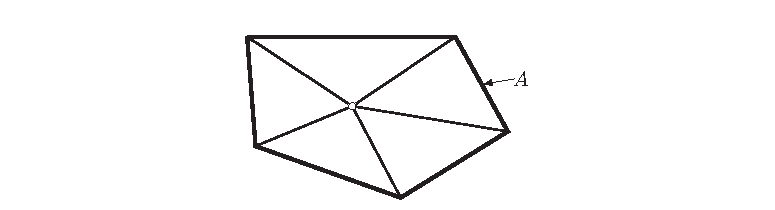
\includegraphics[width=.90\textwidth]{figures/8-12-1.pdf}
\caption*{图 8.12.1}
\end{figure}

\entry{引理}{8.12.2}设 $A$ 为有限复形 $X$ 的满子复形多面体，$C$ 为与 $A$ 不交的单形之并。令
\[U_A=\operatorname{St}(A,\operatorname{sd}X),\qquad
U_C=\operatorname{St}(C,\operatorname{sd}X).\]
则：
\begin{enumerate}[label=(\alph*)]
\item $|X|$ 是 $U_A,U_C,B$ 的不交并，其中
\[B=\overline U_A\setminus U_A=\overline U_C\setminus U_C.\]
\item 以下各包含均为同伦等价：
\[A\to U_A\to\overline U_A\to\operatorname{St}(A,X),\qquad
C\to U_C\to\overline U_C\to\operatorname{St}(C,X).\]
\end{enumerate}

\begin{figure}[htbp]\centering
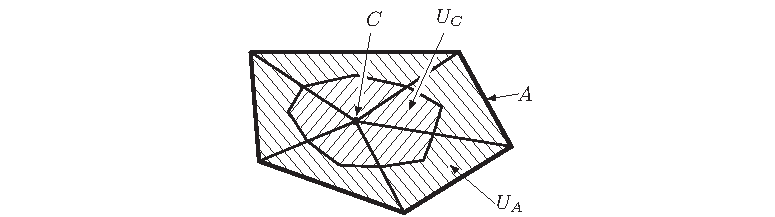
\includegraphics[width=.90\textwidth]{figures/8-12-2.pdf}
\caption*{图 8.12.2}
\end{figure}
\begin{figure}[htbp]\centering
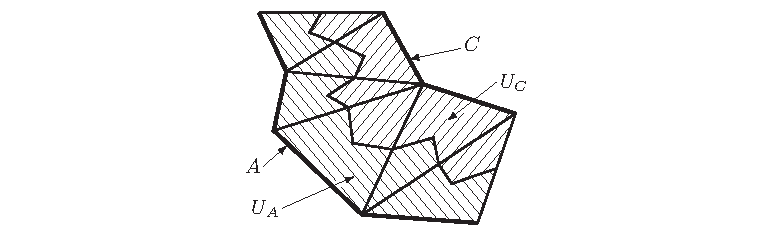
\includegraphics[width=.90\textwidth]{figures/8-12-3.pdf}
\caption*{图 8.12.3}
\end{figure}

\sourcepage{513--514}
\textbf{证明：}设重分后的典型单形为 $s=\widehat\sigma_1\cdots\widehat\sigma_k$，其中 $\sigma_1\succ\cdots\succ\sigma_k$。

第一步：$U_A$ 恰是满足 $\sigma_k\subset A$ 的这些单形内部之并。若最小单形在 $A$ 中，则最小顶点在 $A$ 中，整个开单形位于其星形邻域。反之，若开单形位于 $U_A$ 中，则某个顶点在 $A$ 中，相应单形及其面 $\sigma_k$ 都在 $A$ 中。对 $C$ 同理，所以 $U_A,U_C$ 是不交开集。

第二步：若 $\sigma_k$ 既不属于 $A$ 也不属于 $C$，它必有顶点 $v\in A$、$w\in C$。把 $\widehat v$ 或 $\widehat w$ 添加到上述面链，就得到内部位于 $U_A$ 或 $U_C$ 的单形。公共面 $s$ 因此同时在两个闭包中而不在两个开集中，证明 (a)。

第三步：令 $D=\overline U_A=X\setminus U_C$，证明它是重分后的满子复形多面体，且
\[\operatorname{St}(D,\operatorname{sd}X)=\operatorname{St}(A,X).\]
若一个重分开单形在 $U_C$ 中，其最小顶点就不在 $D$ 中，因而顶点都在 $D$ 的单形必在 $D$ 中。又重心 $\widehat\sigma$ 属于 $D$，当且仅当 $\sigma$ 与 $A$ 相交。若重分单形有顶点在 $D$ 中，其对应原单形有顶点 $v\in A$，则其最大原单形也有此顶点，故该重分开单形位于 $\operatorname{St}(v,X)$ 中。这给出一个包含。反之，原单形 $\sigma$ 若有顶点在 $A$ 中，则 $\widehat\sigma\in D$，而 $\Int\sigma$ 由以该重心为最大顶点的重分开单形组成，均位于 $\operatorname{St}(D,\operatorname{sd}X)$，得到反向包含。

第四步：考察 $A\xrightarrow{i}U_A\xrightarrow{j}D\xrightarrow{k}\operatorname{St}(D,\operatorname{sd}X)$。由于 $A,D$ 为满子复形多面体，$i,k$ 为同伦等价。整个复合也是同伦等价，因为末项等于 $\operatorname{St}(A,X)$。所以 $j$ 也为同伦等价。对 $C$ 同理。\hfill$\square$

\entry{定义}{8.12.3}若 $D\subset X$，且存在拓扑偶 $(X,A)$ 的某个三角剖分，使 $D$ 为其子复形多面体，就称 $D$ 是\emph{$(X,A)$ 中的多面体}。$A$ 为空时，简称 $X$ 中的多面体。

两个集合分别是 $X$ 中的多面体，并不意味着存在同时兼容两者的剖分。例如平面中的横轴与曲线
\[\{(0,0)\}\cup\{(x,x\sin(1/x)):x\ne0\}\]
各自都是多面体，但不存在同时使两者均为子复形多面体的平面剖分。

\entry{引理}{8.12.4}紧致可三角剖分空间 $X$ 中的多面体 $D$，具有任意小的开邻域 $U$，使
\begin{enumerate}[label=(\alph*)]
\item $\overline U$ 与 $X\setminus U$ 都是 $X$ 中的多面体；
\item $D\to U\to\overline U$ 以及
\[X\setminus\overline U\to X\setminus U\to X\setminus D\]
中的各包含均为同伦等价。
\end{enumerate}

\entry{注}{8.12.5}若已选剖分使 $D$ 为满子复形多面体，则对每个 $N\ge1$，$U=\operatorname{St}(D,\operatorname{sd}^NX)$ 都满足这些条件。

\textbf{证明：}只需对第一次重分验证，再任意重分缩小网格即可。上一引理已给出关于 $D$ 的包含。令 $A$ 为与 $D$ 不交的原单形之并，则上一引理中的
\[A\to\operatorname{St}(A,\operatorname{sd}X)\to
\overline{\operatorname{St}(A,\operatorname{sd}X)}\to\operatorname{St}(A,X)\]
依次在后三项等同于 $X\setminus\overline U$、$X\setminus U$、$X\setminus D$，各包含均为同伦等价。\hfill$\square$

\sourcepage{515--516}
\entry{定理}{8.12.6（Lefschetz 对偶的自然形式）}设 $(X,A)$ 是紧致、可三角剖分的相对同调 $n$ 维流形。可以为每个包含 $A$ 的多面体 $D$ 指定同构
\[\lambda_D:H^k(X,D;G)\to H_{n-k}(X\setminus D;G),\]
且它相对于多面体包含自然。可定向时 $G$ 任意，否则取 $G=\Z/2$。

\textbf{证明：}可定向时取定向类 $\Gamma$，否则取模 $2$ 定向类。

第一步：设 $U$ 为 $A$ 的开邻域，且 $\overline U$ 为偶中的多面体，令 $X_U=X\setminus U$。通过相对映射及切除同构，把 $\Gamma$ 限制为
\[\Gamma_U\in H_n(X_U,\Bd U),\qquad\Bd U=\overline U\setminus U.\]
具体是先映到 $H_n(X,\overline U)$，再经包含 $(X_U,\Bd U)\to(X,\overline U)$ 的逆同构。选择兼容剖分，$\Gamma$ 由全部不在 $A$ 中的顶维单形之和代表，其限制就是不在 $U$ 中的单形之和，所以 $\Gamma_U$ 是这个相对流形的定向类。

第二步：对 $D$ 选择引理 8.12.4 的邻域 $U$，并使剖分同时兼容 $A,D,\overline U$。由定理 8.10.10，帽积 $\frown\Gamma_U$ 等于 Lefschetz 同构再复合内部到 $X_U$ 的包含，差一个符号。引理说明该包含是同伦等价，因此帽积本身是同构，且在奇异理论中也如此。

\begin{figure}[htbp]\centering
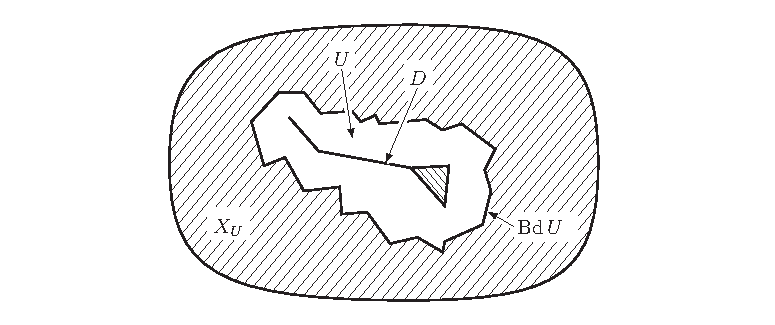
\includegraphics[width=.90\textwidth]{figures/8-12-4.pdf}
\caption*{图 8.12.4}
\end{figure}

在奇异理论中取复合
\[
H^k(X,D)\xleftarrow{i^*}H^k(X,\overline U)
\xrightarrow{k^*}H^k(X_U,\Bd U)
\xrightarrow{\frown\Gamma_U}H_{n-k}(X_U)
\xrightarrow{\ell_*}H_{n-k}(X\setminus D).
\]
其中 $k^*$ 为切除同构；$i^*,\ell_*$ 为同构，因为相应包含是同伦等价。以 $(i^*)^{-1}$ 开始的复合同构记为 $\lambda_{D,U}$。它不依赖所用具体剖分。

第三步：若 $A\subset E\subset D$，选取 $E$ 的合适邻域 $V\subset U$，则 $\lambda_{D,U}$ 与 $\lambda_{E,V}$ 和包含诱导映射交换。比较定义它们的两行复合，在中间插入
\[H^k(X_V,\overline U\setminus V),\qquad X_V=X\setminus V,\]
并用定向类 $\Gamma$ 在这个偶上的限制 $\Gamma'$ 作帽积。所有其余映射均为包含诱导；由帽积自然性，所组成的方块和三角形全部交换，因此得到所需关系。这里必须使用奇异群，因为 $U,V$ 可能不兼容同一个剖分，所插入的偶未必可三角剖分。

\sourcepage{517--518}
\begin{figure}[htbp]\centering
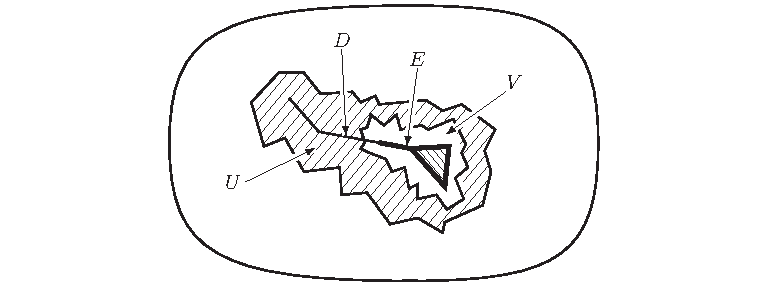
\includegraphics[width=.90\textwidth]{figures/8-12-5.pdf}
\caption*{图 8.12.5}
\end{figure}

第四步：令 $E=D$。对两个合适邻域 $U,U'$，可再选合适 $V\subset U\cap U'$，由第三步
\[\lambda_{D,U}=\lambda_{D,V}=\lambda_{D,U'}.\]
所以可定义 $\lambda_D$ 而不依赖邻域。其自然性同样由第三步得到。\hfill$\square$

\entry{推论}{8.12.7（Alexander 对偶）}固定 $n$，可以给每个 $S^n$ 中的非空真多面体 $A$ 指定同构
\[\alpha_A:\widetilde H^k(A)\to\widetilde H_{n-k-1}(S^n\setminus A),\]
且相对于包含自然。

\textbf{证明：}$k<n-1$ 时，取自然同构的复合 $\lambda_A\delta^*$。$k=n-1$ 时，使用上一节定义同构时的核及交换图，它们同样自然；$k=n$ 时平凡。\hfill$\square$

\subsection*{习题}
\begin{enumerate}
\item 设 $S^n$ 中多面体 $D$ 为不交集合 $A,B$ 的并，$A\approx S^k$，$B\approx S^{n-k-1}$，$0\le k\le n-1$。包含诱导
\[\varphi:\widetilde H_k(A)\to\widetilde H_k(S^n\setminus B),\qquad
\psi:\widetilde H_{n-k-1}(B)\to\widetilde H_{n-k-1}(S^n\setminus A).\]
由 Alexander 对偶，四个群都为无限循环群。证明两个映射差一个符号都是乘以同一整数 $m$。这个整数称为\emph{链环数}，衡量两个球面相互缠绕的次数（参见第 4.9 节习题 3）。〔提示：取剖分使 $A,B$ 满，且没有单形同时与二者相交。令 $C$ 为与 $A$ 不交的单形之并，比较 $B\subset C$ 所诱导的上同调映射及其自然 Alexander 对偶图。〕
\item 解释为什么图 8.12.2、8.12.3 各自实际上都是某个有序偶的“星形”。
\end{enumerate}

\section{Čech 上同调}
\sourcepage{519--520}
至今研究了单纯和奇异两种同调、上同调理论。还有其他理论，其中最著名的是 Čech 理论，尤其在上同调方面表现良好。本节构造其上同调群，证明在可三角剖分空间上与单纯群一致，并给出与奇异群不同的空间。下一节将用它证明推广的 Alexander 对偶。

\entry{定义}{8.13.1}\emph{有向集}是一个带关系 $<$ 的集合 $J$，满足：(1) $\alpha<\alpha$；(2) 若 $\alpha<\beta<\gamma$，则 $\alpha<\gamma$；(3) 任意两个元素都有共同上界，即存在 $\delta$ 使 $\alpha<\delta$、$\beta<\delta$。这里的记号 $<$ 不要求反自反。

\entry{例}{8.13.2}任何全序集在关系 $\le$ 下都是有向集。

\entry{例}{8.13.3}空间所有开覆盖组成有向集：令 $\mathcal A<\mathcal B$ 表示 $\mathcal B$ 加细 $\mathcal A$，即后者每个成员包含于前者某个成员。自反性、传递性显然；两覆盖所有交集 $A\cap B$ 组成共同加细。

\entry{定义}{8.13.4}以有向集 $J$ 为指标的阿贝尔群\emph{直系统}，由群 $G_\alpha$ 及对每个 $\alpha<\beta$ 定义的同态 $f_{\alpha\beta}:G_\alpha\to G_\beta$ 组成，满足
\[f_{\alpha\alpha}=i,\qquad f_{\beta\gamma}f_{\alpha\beta}=f_{\alpha\gamma}.\]

\entry{定义}{8.13.5}在各群的不交并上，令 $g_\alpha\sim g_\beta$，当且仅当存在共同上界 $\delta$，使 $f_{\alpha\delta}(g_\alpha)=f_{\beta\delta}(g_\beta)$。等价类集合称为\emph{直极限}，记为 $\varinjlim_{\alpha\in J}G_\alpha$。其加法定义为
\[\{g_\alpha\}+\{g_\beta\}=\{f_{\alpha\delta}(g_\alpha)+f_{\beta\delta}(g_\beta)\}.\]
容易检验运算定义良好，并使其成为阿贝尔群。若全部结构映射为同构，极限同构于任一群；若对每个 $\alpha$ 都存在 $\beta>\alpha$ 使 $f_{\alpha\beta}=0$，极限为零，特别地结构映射全为零时如此。

\entry{定义}{8.13.6}两个直系统之间的\emph{映射}，包括保序映射 $\varphi:J\to K$ 与同态 $\varphi_\alpha:G_\alpha\to H_{\varphi(\alpha)}$，使结构映射组成的方块交换。它诱导直极限同态
\[\Phi_\to:\varinjlim_JG_\alpha\to\varinjlim_KH_\gamma,\qquad
\{g_\alpha\}\mapsto\{\varphi_\alpha(g_\alpha)\}.\]

\sourcepage{521--522}
\entry{例}{8.13.7}若对固定群 $H$ 有相容同态 $\varphi_\alpha:G_\alpha\to H$，即 $\varphi_\beta f_{\alpha\beta}=\varphi_\alpha$，则诱导 $\varinjlim G_\alpha\to H$。这就是目标直系统只含一个群的特殊情形。

\entry{例}{8.13.8}群序列 $G_1\xrightarrow{f_1}G_2\xrightarrow{f_2}\cdots$ 构成直系统，令 $f_{mn}=f_{n-1}\cdots f_m$。若所有群为 $\Z$，各映射为乘以 $2$，则直极限为二进有理数的加法群
\[\{m/2^r:m\in\Z,\ r\ge0\}.\]
定义 $\varphi_n(m)=m/2^n$，它们相容，所诱导同态容易检验既单又满。

\entry{定义}{8.13.9}若对每个 $\alpha\in J$，都存在 $\delta\in J_0$ 使 $\alpha<\delta$，则称子集 $J_0$ 在 $J$ 中\emph{共尾}。

\entry{引理}{8.13.10}共尾子集本身为有向集，且包含诱导 $\varinjlim_{J_0}G_\alpha\cong\varinjlim_JG_\alpha$。

\textbf{证明：}两个 $J_0$ 中元素先在 $J$ 中取上界，再取 $J_0$ 中更大的元素，即得共同上界。诱导同态满，因为每个元素可向前映到 $J_0$ 的某个群。若 $g_\alpha$（$\alpha\in J_0$）在大极限中为零，则在某个 $G_\delta$ 中像为零；再选 $\epsilon\in J_0$ 大于 $\delta$，其像在 $G_\epsilon$ 中也为零，所以在小极限中已为零。\hfill$\square$

\entry{定义}{8.13.11}对空间的一族子集 $\mathcal A$，定义抽象复形\emph{神经} $N(\mathcal A)$：顶点为该族成员，有限子族组成单形，当且仅当其交非空。

若 $\mathcal B$ 加细 $\mathcal A$，为每个 $B$ 选取包含它的 $g(B)\in\mathcal A$，得到单纯映射 $g:N(\mathcal B)\to N(\mathcal A)$。不同选择彼此邻接，因为
\[\bigcap B_i\subset\bigcap\bigl(g(B_i)\cap g'(B_i)\bigr),\]
所以诱导相同同调和上同调同态。

\entry{定义}{8.13.12}这些唯一确定的同态称为\emph{加细诱导的同态}：
\[g_*:H_k(N(\mathcal B);G)\to H_k(N(\mathcal A);G),\qquad
g^*:H^k(N(\mathcal A);G)\to H^k(N(\mathcal B);G).\]

\sourcepage{523--524}
\entry{定义}{8.13.13}令 $J$ 为 $X$ 所有开覆盖按加细关系组成的有向集。给每个覆盖指定 $H^k(N(\mathcal A);G)$，以加细诱导映射为结构映射，定义
\[\check H^k(X;G)=\varinjlim_{\mathcal A\in J}H^k(N(\mathcal A);G),\]
称为\emph{Čech 上同调}。以约化群取直极限，定义约化版本 $\check{\widetilde H}^{,k}(X;G)$。这些群仅依赖于开覆盖族，显然是拓扑不变量。

\entry{定理}{8.13.14}对任意单纯复形 $K$，$\check H^k(|K|;G)\cong H^k(K;G)$，约化版本也成立。

\textbf{证明：}以各顶点开星形邻域组成覆盖 $\mathcal A(K)$。对应 $v\mapsto\operatorname{St}v$ 给出 $K\cong N(\mathcal A(K))$，因为若干顶点张成单形当且仅当其开星形邻域交非空。

若 $K'$ 重分 $K$，恒等映射的单纯逼近 $h:K'\to K$ 满足
\[\operatorname{St}(w,K')\subset\operatorname{St}(h(w),K).\]
同一对应给出神经间的加细映射，两边与上述同构组成交换图。诱导的四个上同调映射全为同构。所有重分的星形覆盖在所有开覆盖中共尾，这是一般单纯逼近定理的结论（有限复形只需有限情形）。因此 Čech 群等于各重分上同调群的直极限；所有结构映射是同构，故极限等于 $H^k(K;G)$。\hfill$\square$

为计算一般空间，需要证明 Čech 上同调的“连续性”，先证一个引理。

\entry{引理}{8.13.15}设 $Y$ 为正规空间 $X$ 的紧致子空间。令 $L$ 为由 $X$ 中开集覆盖 $Y$ 的所有覆盖组成的有向集，则
\[\check H^k(Y;G)\cong\varinjlim_{\mathcal A\in L}H^k(N(\mathcal A);G).\]
约化版本亦然。

\textbf{证明：}第一步：正规空间的有限开覆盖 $U_1,\ldots,U_r$ 可缩小为开覆盖 $V_1,\ldots,V_r$，使 $\overline V_i\subset U_i$。先在 $U_1$ 中取包含闭集 $X\setminus(U_2\cup\cdots\cup U_r)$ 的开集 $V_1$，并使闭包仍在 $U_1$；替换后仍覆盖。再对第二项重复，依次完成。

第二步：称同指标族 $\{C_i\},\{D_i\}$ 的神经\emph{自然同构}，若每个对应有限交同时为空或非空。我们证明：有限闭集族 $C_i\subset U_i$，其中 $U_i$ 开，可以扩张为 $C_i\subset W_i\subset\overline W_i\subset U_i$，且 $\{C_i\}$ 与 $\{\overline W_i\}$ 的神经自然同构。

\sourcepage{525--526}
先把所有与 $C_1$ 不交的有限交 $C_{i_1}\cap\cdots\cap C_{i_p}$ 取并，得到与 $C_1$ 不交的闭集 $E$。正规性允许选择 $W_1$，使其包含 $C_1$、闭包包含于 $U_1$ 且避开 $E$。于是用 $\overline W_1$ 替换 $C_1$ 不改变神经：原来非空的交仍非空，原来为空的交因包含于 $E$ 而仍为空。然后逐项替换，完成构造。

第三步：称有限环境开覆盖 $\mathcal W$ \emph{适配于 $Y$}，若 $N(\mathcal W)$ 与限制覆盖 $N(\mathcal W\cap Y)$ 自然同构。证明这些覆盖组成的子族 $L_0$ 共尾。任取覆盖，先取有限子覆盖 $U_i$；在正规空间 $Y$ 中用第一步缩小，令闭集 $C_i=\overline V_i\subset U_i\cap Y$ 仍覆盖 $Y$；再用第二步在 $X$ 中扩张成 $W_i$。有限交是否非空，沿包含关系
\[\bigcap C_i\subset\bigcap W_i\cap Y\subset\bigcap W_i\subset\bigcap\overline W_i\]
具有相同答案，因为首末两项同时为空或非空。因此覆盖适配于 $Y$，并加细原覆盖。

第四步：令 $J$ 为 $Y$ 的所有自身开覆盖，$J_0$ 为适配环境覆盖限制到 $Y$ 所得的覆盖。每个 $Y$ 中开覆盖都来自环境开覆盖的限制，所以 $J_0$ 在 $J$ 中也共尾。因此先限制到 $J_0$，再使用自然神经同构，最后用 $L_0$ 在 $L$ 中共尾，依次得到
\[\check H^k(Y;G)\cong\varinjlim_{J_0}H^k(N(\mathcal W\cap Y);G)
\cong\varinjlim_{L_0}H^k(N(\mathcal W);G)
\cong\varinjlim_LH^k(N(\mathcal A);G).\]
\hfill$\square$

\entry{定理}{8.13.16}设 $X$ 紧致且可三角剖分，$D_1\supset D_2\supset\cdots$ 为其中多面体，交为 $Y$。则
\[\check H^k(Y;G)\cong\varinjlim_nH^k(D_n;G),\]
约化版本也成立。

\textbf{证明：}省略系数。选择 $X$ 的剖分 $X_n$，使 $D_n$ 为满子复形 $K_n$ 的多面体、网格小于 $1/n$，并使从下一剖分到底层前一剖分的恒等映射满足星形条件。直极限不依赖于各多面体的具体剖分，所以可用 $H^k(K_n)$ 计算。

第一步：令 $\mathcal A'_n=\{\operatorname{St}(v,K_n):v\in K_n\}$。与定理 8.13.14 相同，$K_n\cong N(\mathcal A'_n)$。包含的单纯逼近 $h:K_{n+1}\to K_n$ 诱导对应的神经映射，且交换图相容，所以
\[\varinjlim H^k(K_n)\cong\varinjlim H^k(N(\mathcal A'_n)).\]
这里不能把极限等同于某个固定群，因为 $h^*$ 未必为同构。

\sourcepage{527--528}
第二步：改用环境开覆盖 $\mathcal A_n=\{\operatorname{St}(v,X_n):v\in K_n\}$。由星形条件，后一覆盖加细前一覆盖。它与 $\mathcal A'_n$ 的神经自然同构：一个方向由包含显然；另一个方向，若环境星形邻域交非空，则对应顶点张成 $X_n$ 的单形；这些顶点都在满子复形 $K_n$ 中，故单形也在其中。因此 $\varinjlim H^k(N(\mathcal A'_n))\cong\varinjlim H^k(N(\mathcal A_n))$。

第三步：证明 $\{\mathcal A_n\}$ 在 $Y$ 的全部环境开覆盖中共尾。使用 Lebesgue 数引理的加强形式：若紧集 $D$ 被环境开集覆盖，则存在 $\delta>0$，使任何与 $D$ 相交且直径小于 $\delta$ 的集合都包含于某个覆盖成员。

任取 $Y$ 的环境开覆盖，它必覆盖某个 $D_N$。否则可选 $x_n\in D_n$ 不被覆盖，由紧致性取收敛子列，其极限必在交集 $Y$ 中，与开覆盖包含 $Y$ 的一个邻域矛盾。对 $D_N$ 选上述 $\delta$，再取 $m>N$ 使 $2/m<\delta$。$\mathcal A_m$ 的每个成员直径不超过 $2/m$，且含有 $D_m\subset D_N$ 中顶点，故加细给定覆盖。

第四步：结合前三步，$\varinjlim H^k(D_n)$ 同构于全部环境开覆盖神经上同调的直极限，上一引理将其等同于 $\check H^k(Y)$。\hfill$\square$

下面计算一个不可三角剖分空间。

\entry{推论}{8.13.17}设 $X$ 为闭拓扑学家正弦曲线（定义 4.6.5），则
\[H^1(X)=0\quad\text{（奇异上同调）},\qquad\check H^1(X)\cong\Z.\]

\sourcepage{529--530}
\textbf{证明：}为方便起见，用图 8.13.1 的折线模型表示该空间。令 $U=X\cap\{y>1/8\}$、$V=X\cap\{y<3/8\}$。奇异 Mayer--Vietoris 序列给出
\[H_1(U)\oplus H_1(V)\to H_1(X)\to\widetilde H_0(U\cap V)
\to\widetilde H_0(U)\oplus\widetilde H_0(V).\]
$V$ 同胚于开区间，故其相关群为零。$U$ 有两个道路分支，分别同胚于开区间与半开区间，故 $H_1(U)=0$，其约化零维群由 $q-p$ 生成，其中 $p=(0,1/4)$、$q=(1,1/4)$。交集是两个不交开线段，约化零维群也由同一链生成，所以最后一个映射为同构，得到 $H_1(X)=0$。泛系数定理给出 $H^1(X)=0$；也可直接用上同调的 Mayer--Vietoris 序列。

\begin{figure}[htbp]\centering
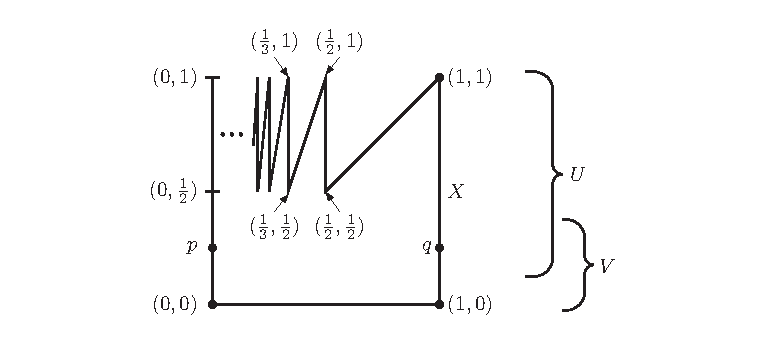
\includegraphics[width=.96\textwidth]{figures/8-13-1.pdf}
\caption*{图 8.13.1}
\end{figure}

再令 $C_n$ 为图 8.13.2 的闭矩形，$D_n=X\cup C_n$。每个 $D_n$ 是多面体，同伦等价于圆，故 $H^1(D_n)\cong\Z$。而 $D_{n+1}$ 是 $D_n$ 的形变收缩核，包含诱导同构。由连续性定理，$\check H^1(X)\cong\varinjlim H^1(D_n)\cong\Z$。\hfill$\square$

\begin{figure}[htbp]\centering
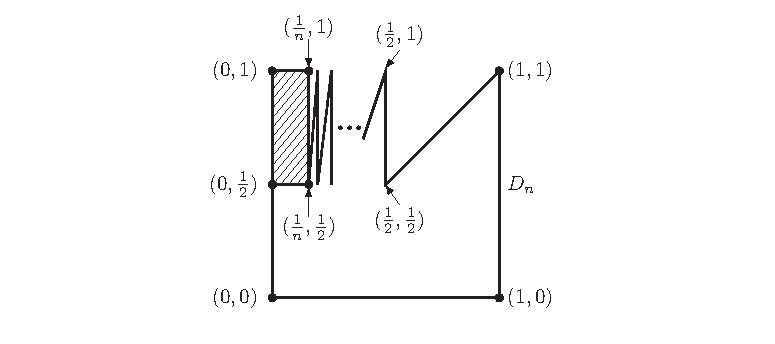
\includegraphics[width=.96\textwidth]{figures/8-13-2.pdf}
\caption*{图 8.13.2}
\end{figure}

这里只初步接触 Čech 上同调。完整理论还需定义连续映射诱导的同态（容易），推广到偶，并验证 Eilenberg--Steenrod 公理（需要一定工作）。参见 [ES52] 第 9、10 章。

\sourcepage{530--531}
\subsection*{习题}
\begin{enumerate}
\item 验证例 8.13.8 的细节。
\item 令 $\mu_n:\Z\to\Z$ 为乘以 $n$。直系统 $\Z\xrightarrow{\mu_2}\Z\xrightarrow{\mu_3}\Z\xrightarrow{\mu_4}\cdots$ 的极限是哪个熟悉的群？
\item 验证定义 Čech 上同调所用的群及同态确实组成直系统。
\item 验证连续性定理证明中引用的加强 Lebesgue 数引理。
\item 设 $X=B^2\times S^1$ 为实心环面，$f:X\to X$ 为图 8.13.3 中的嵌入。令 $X_0=X$，$X_{n+1}=f(X_n)$，$S=\bigcap X_n$，称为\emph{螺线管空间}（solenoid）。(a) 描述 $X_2$；(b) 计算 $\check H^1(S)$。
\begin{figure}[htbp]\centering
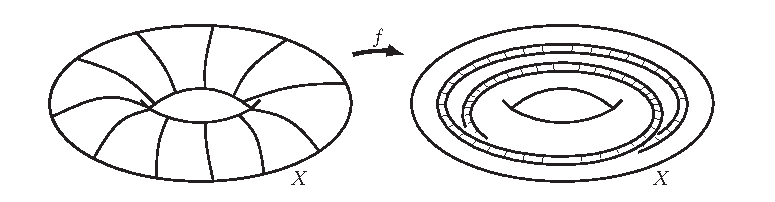
\includegraphics[width=.96\textwidth]{figures/8-13-3.pdf}
\caption*{图 8.13.3}
\end{figure}
\item 令 $\mathcal C$ 为 $X$ 的紧致子空间族，以包含定向。证明它为有向集，令 $G_C=H_i(C)$，结构映射为包含诱导同态，证明
\[H_i(X)\cong\varinjlim_{C\in\mathcal C}H_i(C).\]
这是奇异同调紧支集性质的另一种表述。\translatornote{原文等式左端下标写作 $1$，由所定义直系统应为 $i$。}
\item 对任意集合 $X$，说明如何使其幂集成为有向集。
\end{enumerate}

\section{Alexander--Pontryagin 对偶}
\sourcepage{531--532}
现在证明推广的 Alexander 对偶。它适用于球面中任意闭子集，而不限于多面体。作为应用，得到比此前更一般的 Jordan 曲线定理。

\entry{定理}{8.14.1（Alexander--Pontryagin 对偶）}若 $A$ 是 $S^n$ 的非空真闭子集，则
\[\check{\widetilde H}^{\,k}(A)\cong\widetilde H_{n-k-1}(S^n\setminus A).\]
左边为 Čech 上同调，右边为奇异同调。

\textbf{证明：}选取球面剖分 $X$，细到不是每个单形都与 $A$ 相交。令 $A_m$ 为 $\operatorname{sd}^mX$ 中所有与 $A$ 相交的单形及其面组成的子复形。则 $|A_m|$ 为非空真多面体，递减且交为 $A$。

自然 Alexander 对偶给出相容同构
\[\alpha_m:\widetilde H^k(A_m;G)\to\widetilde H_{n-k-1}(X\setminus|A_m|;G),\]
因而诱导两端直极限的同构。左端极限由定理 8.13.16 等于约化 Čech 上同调。右端由奇异同调的紧支集性质等于补空间的约化奇异同调：每个奇异闭链承载于紧集，故位于某个递增开集 $X\setminus|A_m|$；若两个闭链在整个补空间同调，连接它们的有限奇异链也承载于某个这样的开集。所以包含诱导的极限同态既满又单。\hfill$\square$

\entry{推论}{8.14.2}设 $n>1$，$M$ 是紧致连通、可三角剖分的 $(n-1)$ 维流形，$h:M\to S^n$ 是嵌入。则 $M$ 可定向，补空间恰有两个道路分支，且 $h(M)$ 为其公共边界。

\sourcepage{533--534}
\textbf{证明：}由对偶，$\check H^{n-1}(M)\cong\widetilde H_0(S^n\setminus h(M))$。因 $M$ 可三角剖分，Čech 群与单纯群一致。若不可定向，左端为 $\Z/2$，但右端自由阿贝尔，矛盾。因此可定向，左端为 $\Z$，补空间有两个道路分支 $U,V$。

公共边界的论证同 Jordan 定理：从 $M$ 删去小顶维单形的内部，所得 $M_0=h(M\setminus\Int s)$ 不分割球面，因为
\[\widetilde H_0(S^n\setminus M_0)\cong\check H^{n-1}(M_0)
\cong H^{n-1}(M_0)=0.\]
因此可以经过任意小的这种缺口连接两侧，得到公共边界结论。\hfill$\square$

\begin{figure}[htbp]\centering
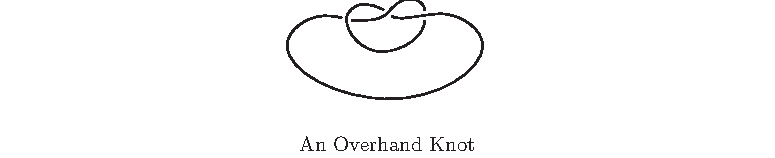
\includegraphics[width=.90\textwidth]{figures/8-14-1.pdf}
\caption*{图 8.14.1：单结（overhand knot）}
\end{figure}

\subsection*{习题}
\begin{enumerate}
\item 设 $X$ 为闭拓扑学家正弦曲线，$f:X\to S^n$ 为嵌入。计算 $\widetilde H_i(S^n\setminus f(X))$。
\item 证明若把 Čech 上同调换成奇异上同调，Alexander--Pontryagin 对偶不成立。
\item 证明 Klein 瓶与射影平面均不能嵌入 $\R^3$，但都可嵌入 $\R^4$。〔提示：从射影平面删去一个开圆盘，剩余部分是什么？〕
\item 若 $A,B$ 为 $S^n$ 的同胚闭子集，证明对所有 $i$，$H_i(S^n\setminus A)\cong H_i(S^n\setminus B)$。注意补空间本身不一定同胚。图 8.14.1 给出圆在三维球面中的一个嵌入，称为单结，其补空间与标准圆嵌入的补空间同调群相同，但基本群不同，故不同胚（见 [CF77] 第 6 章）。
\item 说明推论 8.14.2 为何推广了 Jordan 曲线定理，并说明它为何不与 Alexander 角状球面矛盾（第 4.9 节）。
\end{enumerate}

\backmatter
\chapter*{延伸阅读}
\addcontentsline{toc}{chapter}{延伸阅读}
\sourcepage{535}
\begin{description}
\item[{[Bou16]}] N. Bourbaki，《代数拓扑》（\textit{Topologie Algébrique}），Springer，Heidelberg，2016。
\item[{[Ful95]}] William Fulton，《代数拓扑初步》（\textit{Algebraic Topology: A First Course}），Springer，New York，1995。
\item[{[GH81]}] Marvin J. Greenberg、John R. Harper，《代数拓扑初步》，CRC Press，Boca Raton，1981。
\item[{[Hat02]}] Allen Hatcher，《代数拓扑》（\textit{Algebraic Topology}），Cambridge University Press，Cambridge，2001。
\item[{[Spa94]}] Edwin H. Spanier，《代数拓扑》，Springer，New York，1994。
\item[{[Wei14]}] Steven H. Weintraub，《代数拓扑基础》（\textit{Fundamentals of Algebraic Topology}），Springer，New York，2016。
\end{description}
\translatornote{本页文献代号与年份按原书保留，部分代号中的年份与所列出版年份不同。}

\chapter*{人物资料}
\addcontentsline{toc}{chapter}{人物资料}
\sourcepage{537--539}
以下保留姓名的原文拼写，以便与定理名称及参考文献对照。出生日期及“生于”等措辞均按原书记载。
\begin{description}[style=nextline]
\item[Abel, Niels Henrik] 1802 年 8 月 5 日—1829 年 4 月 6 日。
\item[Alexander, James Waddell, II] 1888 年 9 月 19 日—1971 年 9 月 23 日。多数著作署名 J. W. Alexander。
\item[Alexandrov, Pavel Sergeyevich] 1896 年 5 月 7 日—1982 年 11 月 16 日。常译写为 Paul Alexandroff；发表著作时至少使用过 16 种姓名形式。
\item[Betti, Enrico] 1823 年 10 月 21 日—1892 年 8 月 11 日。
\item[Bokshtein, Meer Feliksovich] 1913 年 10 月 4 日—1990 年 5 月 2 日。曾署名 M. F. Bokšteĭn、M. Bockstein、M. Bokšteĭn 和 Meyer Bockstein。
\item[Borsuk, Karol] 1905 年 5 月 8 日—1982 年 1 月 24 日。
\item[Brouwer, Luitzen Egbertus Jan] 1881 年 2 月 27 日—1966 年 12 月 2 日。几乎所有著作均署名 L. E. J. Brouwer。
\item[Brown, Morton] 生于 1931 年 8 月 12 日。
\item[Cannon, James Weldon] 1943 年 1 月 30 日出生。
\item[Čech, Eduard] 1893 年 6 月 29 日—1960 年 3 月 15 日。
\item[De Morgan, Augustus] 1806 年 6 月 27 日—1871 年 3 月 18 日。
\item[Edwards, Robert Duncan] 生于 1942 年。
\item[Eilenberg, Samuel] 1913 年 9 月 30 日—1998 年 1 月 30 日。
\item[Euler, Leonhard] 1707 年 4 月 15 日—1783 年 9 月 18 日。
\item[Hausdorff, Felix] 1868 年 11 月 8 日—1942 年 1 月 26 日。
\item[Hurewicz, Witold] 1904 年 6 月 29 日—1956 年 9 月 6 日。
\item[Hilbert, David] 1862 年 1 月 23 日—1943 年 2 月 14 日。
\item[Hopf, Heinz] 1894 年 11 月 19 日—1971 年 6 月 3 日。
\item[Jordan, Marie Ennemond Camille] 1838 年 1 月 5 日—1922 年 1 月 22 日。几乎所有著作均署名 Camille Jordan。
\item[Klein, Felix Christian] 1849 年 4 月 25 日—1925 年 6 月 22 日。发表著作时署名 Felix Klein。
\item[Kronecker, Leopold] 1823 年 12 月 7 日—1891 年 12 月 29 日。
\item[Künneth, Hermann Lorenz] 1892 年 7 月 6 日—1975 年 5 月 7 日。署名 Hermann Künneth。
\item[Lebesgue, Henri Léon] 1875 年 6 月 28 日—1941 年 7 月 26 日。几乎所有著作均署名 Henri Lebesgue。
\item[Lefschetz, Solomon] 1884 年 9 月 3 日—1972 年 10 月 5 日。
\item[MacLane, Leslie Saunders] 1909 年 8 月 4 日—2005 年 4 月 14 日。多数著作署名 Saunders Mac Lane，也常将姓拼作 MacLane；少数仅用首字母 S.，不使用 Leslie。
\item[Mayer, Walther] 1887 年 3 月 11 日—1948 年 9 月 10 日。
\item[Mazur, Barry Charles] 生于 1937 年 12 月 19 日。多数著作署名 Barry Mazur。
\item[Möbius, August Ferdinand] 1790 年 11 月 17 日—1868 年 9 月 26 日。在《纯粹与应用数学杂志》发表的文章署名 A. F. Mobius。
\item[Moise, Edwin Evariste] 1918 年 12 月 22 日—1998 年 12 月 18 日。多数著作署名 Edwin E. Moise。
\item[Morse, Harold Calvin Marston] 1892 年 3 月 24 日—1977 年 6 月 22 日。几乎所有著作均署名 Marston Morse。
\item[Noether, Amalie Emmy] 1882 年 3 月 23 日—1935 年 4 月 14 日。几乎所有著作均署名 Emmy Noether。
\item[Peano, Giuseppe] 1858 年 8 月 27 日—1932 年 4 月 20 日。
\item[Poincaré, Jules Henri] 1854 年 4 月 29 日—1912 年 7 月 17 日。几乎所有著作均署名 Henri Poincaré 或 H. Poincaré。
\item[Pontryagin, Lev Semenovich] 1908 年 9 月 3 日—1988 年 5 月 3 日。多数著作署名 L. S. Pontryagin 或 L. S. Pontrjagin。
\item[Reidemeister, Kurt Werner Friedrich] 1893 年 10 月 13 日—1971 年 7 月 8 日。
\item[Riemann, Georg Friedrich Bernhard] 1826 年 9 月 17 日—1866 年 7 月 20 日。署名 Bernhard Riemann。
\item[Schoenflies, Artur Moritz] 1853 年 4 月 17 日—1928 年 5 月 27 日。曾署名 Artur Schoenflies、A. Schoenflies 和 A. Schönflies。
\item[Steenrod, Norman Earl] 1910 年 4 月 22 日—1971 年 10 月 14 日。多数著作署名 N. E. Steenrod。
\item[Stone, Marshall Harvey] 1903 年 4 月 8 日—1989 年 1 月 9 日。多数著作署名 M. H. Stone。
\item[Tietze, Heinrich Franz Friedrich] 1880 年 8 月 31 日—1964 年 2 月 17 日。几乎所有著作均署名 Heinrich Tietze。
\item[Ulam, Stanisław Marcin] 1909 年 4 月 13 日—1984 年 5 月 13 日。多数著作署名 S. M. Ulam 或 S. Ulam。
\item[Urysohn, Pavel Samuilovich] 1898 年 2 月 3 日—1924 年 8 月 17 日。\translatornote{原书把“多数著作署名 S. M. Ulam 或 S. Ulam”排在本条之后；这显然属于上一条 Ulam，此处调整归属。}
\item[Vietoris, Leopold] 1891 年 6 月 4 日—2002 年 4 月 9 日。
\item[Weyl, Hermann Klaus Hugo] 1885 年 11 月 9 日—1955 年 12 月 8 日。署名 Hermann Weyl。
\item[Whitehead, John Henry Constantine] 1904 年 11 月 11 日—1960 年 5 月 8 日。几乎所有著作均署名 J. H. C. Whitehead。
\item[Whitney, Hassler] 1907 年 3 月 23 日—1989 年 5 月 10 日。
\item[Zilber, Joseph Abraham] 1923 年 7 月 27 日—2009 年 10 月 4 日。多数著作署名 J. A. Zilber。
\item[Zorn, Max August] 1906 年 6 月 6 日—1993 年 3 月 9 日。
\end{description}

\chapter*{参考文献}
\addcontentsline{toc}{chapter}{参考文献}
\sourcepage{541--543}
文献代号、作者、期刊和出版信息按原书保留；题名后附中文译名。
\begin{description}[style=nextline]
\item[{[Ale24]}] James Waddell Alexander. \textit{An example of a simply connected surface bounding a region which is not simply connected}（围成非单连通区域的单连通曲面之例）. Proc. Nat. Acad. Sci. U.S.A., 10:8--10, 1924.
\item[{[Bro60]}] Morton Brown. \textit{A proof of the generalized Schoenflies theorem}（广义 Schoenflies 定理的证明）. Bull. Amer. Math. Soc., 66:74--76, 1960.
\item[{[Bro62]}] Morton Brown. \textit{Locally flat imbeddings of topological manifolds}（拓扑流形的局部平坦嵌入）. Ann. of Math. (2), 75:331--341, 1962.
\item[{[Can79]}] J. W. Cannon. \textit{Shrinking cell-like decompositions of manifolds. Codimension three}（流形类胞腔分解的收缩：余维三）. Ann. of Math. (2), 110(1):83--112, 1979.
\item[{[CF77]}] Richard H. Crowell、Ralph H. Fox. \textit{Introduction to knot theory}（纽结理论导引），Graduate Texts in Mathematics 57，Springer-Verlag，New York--Heidelberg，1977；1963 年原版重印。
\item[{[Dol95]}] Albrecht Dold. \textit{Lectures on algebraic topology}（代数拓扑讲义），Classics in Mathematics，Springer-Verlag，Berlin，1995；1972 年版重印。
\item[{[EM53]}] Samuel Eilenberg、Saunders MacLane. \textit{Acyclic models}（无环模型）. Amer. J. Math., 75:189--199, 1953.
\item[{[ES52]}] Samuel Eilenberg、Norman Steenrod. \textit{Foundations of algebraic topology}（代数拓扑基础），Princeton University Press，Princeton，1952。
\item[{[EZ53]}] Samuel Eilenberg、J. A. Zilber. \textit{On products of complexes}（论复形的乘积）. Amer. J. Math., 75:200--204, 1953.
\item[{[Fuc71]}] Martin Fuchs. \textit{A note on mapping cylinders}（关于映射柱的一则注记）. Michigan Math. J., 18:289--290, 1971.
\item[{[GH81]}] Marvin J. Greenberg、John R. Harper. \textit{Algebraic topology: A first course}（代数拓扑初步），Mathematics Lecture Note Series，CRC Press，Boca Raton，1981。
\item[{[Hil91]}] David Hilbert. \textit{Ueber die stetige Abbildung einer Linie auf ein Flächenstück}（论线到平面区域的连续映射）. Math. Ann., 38(3):459--460, 1891.
\item[{[Hop28]}] Heinz Hopf. \textit{Eine Verallgemeinerung der Euler--Poincaréschen Formel}（Euler--Poincaré 公式的推广）. Nachr. Akad. Wiss. Göttingen Math.-Phys. Kl. II, 127--136, 1928.
\item[{[Jor14]}] Camille Jordan. \textit{Cours d'analyse de l'école polytechnique. Tome III}（巴黎综合理工学院分析教程，第三卷），Cambridge Library Collection--Mathematics，Cambridge University Press，2014。内容为积分学与微分方程，1887 年第一版重印。
\item[{[Kne25]}] H. Kneser. \textit{Die Topologie der Mannigfaltigkeiten}（流形的拓扑）. Jahresber. Dtsch. Math.-Ver., 34:1--14, 1925.
\item[{[Man14]}] Ciprian Manolescu. \textit{Triangulations of manifolds}（流形的三角剖分）. ICCM Not., 2(2):21--23, 2014.
\item[{[Mas91]}] William S. Massey. \textit{A basic course in algebraic topology}（代数拓扑基础教程），Graduate Texts in Mathematics 127，Springer-Verlag，New York，1991。
\item[{[Maz59]}] Barry Mazur. \textit{On embeddings of spheres}（论球面的嵌入）. Bull. Amer. Math. Soc., 65:59--65, 1959.
\item[{[Maz61]}] B. C. Mazur. \textit{On embeddings of spheres}（论球面的嵌入）. Acta Math., 105:1--17, 1961.
\item[{[ML63]}] Saunders Mac Lane. \textit{Homology}（同调），Die Grundlehren der mathematischen Wissenschaften 114，Springer-Verlag，Berlin--Göttingen--Heidelberg；Academic Press，New York，1963。
\item[{[Moi52]}] Edwin E. Moise. \textit{Affine structures in 3-manifolds. V. The triangulation theorem and Hauptvermutung}（三维流形的仿射结构之五：三角剖分定理与主猜想）. Ann. of Math. (2), 56:96--114, 1952.
\item[{[Mor60]}] Marston Morse. \textit{A reduction of the Schoenflies extension problem}（Schoenflies 延拓问题的化简）. Bull. Amer. Math. Soc., 66:113--115, 1960.
\item[{[Mun00]}] James R. Munkres. \textit{Topology}（拓扑学），第二版，Prentice Hall，Upper Saddle River，2000。
\item[{[New51]}] M. H. A. Newman. \textit{Elements of the topology of plane sets of points}（平面点集拓扑基础），第二版，Cambridge University Press，1951。
\item[{[Pea90]}] G. Peano. \textit{Sur une courbe, qui remplit toute une aire plane}（论一条填满整个平面区域的曲线）. Math. Ann., 36(1):157--160, 1890.
\item[{[Poi10]}] Henri Poincaré. \textit{Papers on topology}（拓扑学论文集），History of Mathematics 37，American Mathematical Society，Providence；London Mathematical Society，London，2010。收录《位置分析》及五篇续篇，John Stillwell 翻译并撰写导言。
\item[{[Rei35]}] Kurt Reidemeister. \textit{Homotopieringe und Linsenräume}（同伦环与透镜空间）. Abh. Math. Sem. Univ. Hamburg, 11(1):102--109, 1935.
\item[{[Spa94]}] Edwin H. Spanier. \textit{Algebraic topology}（代数拓扑），Springer-Verlag，New York，1994；修订第三版重印。
\item[{[ST80]}] Herbert Seifert、William Threlfall. \textit{Seifert and Threlfall: a textbook of topology}（Seifert--Threlfall 拓扑学教材），Pure and Applied Mathematics 89，Academic Press，New York--London，1980。Joan S. Birman 作序，附 Seifert《三维纤维空间的拓扑》，Wolfgang Heil 从德文译出。
\item[{[Vic73]}] James W. Vick. \textit{Homology theory}（同调论：代数拓扑导引），Pure and Applied Mathematics 53，Academic Press，New York--London，1973。
\item[{[Vic94]}] James W. Vick. \textit{Homology theory}（同调论：代数拓扑导引），第二版，Graduate Texts in Mathematics 145，Springer-Verlag，New York，1994。
\item[{[Wey64]}] Hermann Weyl. \textit{The concept of a Riemann surface}（Riemann 曲面的概念），ADIWES International Series in Mathematics，Addison-Wesley，Reading--London，1964，德文版译本。
\item[{[Whi49]}] J. H. C. Whitehead. \textit{Combinatorial homotopy. I}（组合同伦，第一部分）. Bull. Amer. Math. Soc., 55:213--245, 1949.
\item[{[Whi78]}] George W. Whitehead. \textit{Elements of homotopy theory}（同伦理论基础），Graduate Texts in Mathematics 61，Springer-Verlag，New York--Berlin，1978。
\end{description}

\chapter*{符号索引}
\addcontentsline{toc}{chapter}{符号索引}
\sourcepage{545--556}
下列数字均为原书页码。相同符号在不同上下文中可能有不同含义；本索引按原书出现顺序排列。
\begingroup\small
\newcommand{\nirow}[3]{\noindent\( #1 \)\quad #2\hfill #3\par\smallskip}
\nirow{\R^N}{欧氏空间}{2}
\nirow{0,\ \|x\|}{欧氏原点；欧氏范数}{2}
\nirow{\Bd\sigma,\ \Int\sigma}{单形的边界、内部}{5}
\nirow{B^n}{实 $n$ 维空间中的闭单位球}{5}
\nirow{S^n}{单位球面}{5}
\nirow{E^{n-1}_+,\ E^{n-1}_-}{上、下单位半球}{5}
\nirow{\overline A,\ \Int A,\ \Bd A}{拓扑闭包、内部、边界}{6}
\nirow{K^{(p)},\ |K|}{单纯复形的 $p$ 维骨架、多面体}{9}
\nirow{t_v(x)}{点 $x$ 关于顶点 $v$ 的重心坐标}{11}
\nirow{\operatorname{St}v,\ \overline{\operatorname{St}}v,\ \operatorname{Lk}v}{顶点的星形邻域、闭星形邻域、链环}{12}
\nirow{E^J,\ |x-y|,\ \dim K}{广义欧氏空间、其度量、复形维数}{15}
\nirow{P^2}{射影平面}{20}
\nirow{0,\ \Z,\ \mathbb Q,\ \mathbb C}{阿贝尔群单位元；整数、有理数、复数}{23}
\nirow{\ker f,\ \operatorname{im}f,\ \operatorname{cok}f}{同态的核、像、余核}{24}
\nirow{\cong}{同构}{24}
\nirow{\bigoplus_{\alpha\in J}G_\alpha,\ \prod_{\alpha\in J}G_\alpha}{群的直和、直积}{25、26}
\nirow{\Z/n}{模 $n$ 整数}{27}
\nirow{v_0\cdots v_p,\ [v_0,\ldots,v_p]}{单形、有向单形}{30}
\nirow{C_p(K)}{单纯链群}{31}
\nirow{\partial_p:C_p(K)\to C_{p-1}(K)}{单纯边缘算子}{32}
\nirow{Z_p(K),\ B_p(K)}{单纯闭链群、边界群}{34}
\nirow{H_p(K)}{单纯同调群}{35}
\nirow{C_p^\infty(K)}{无限链群}{37}
\nirow{\partial_p^\infty,\ H_p^\infty(K)}{无限链边缘算子、同调群}{38}
\nirow{\partial}{省略维数下标的边缘算子}{40}
\nirow{S_1\mathbin{\#}S_2}{曲面的连通和}{44}
\nirow{\epsilon:C_0(K)\to\Z,\ \widetilde H_p(K)}{单纯增广、约化同调}{50}
\nirow{w*K}{以 $w$ 为顶点的锥}{51}
\nirow{[w,c_p]}{单纯括号运算}{53}
\nirow{S(K)}{复形的悬挂}{55}
\nirow{(K,K_0),\ C_p(K,K_0)}{单纯偶、相对单纯链群}{56}
\nirow{Z_p(K,K_0),\ B_p(K,K_0),\ H_p(K,K_0)}{相对闭链、边界、同调群}{57}
\nirow{C_p(K;G),\ Z_p(K;G),\ B_p(K;G),\ H_p(K;G)}{$G$ 系数的单纯链、闭链、边界、同调群}{61}
\nirow{H_p(K,K_0;G)}{$G$ 系数相对单纯同调群}{61}
\nirow{H_p(C),\ W_p}{链复形同调群、弱边界子群}{69}
\nirow{T_p(C)}{同调群的挠子群}{70}
\nirow{f_\#:C_p(K)\to C_p(L)}{单纯映射诱导的链映射}{73}
\nirow{f_*:H_p(K)\to H_p(L)}{单纯映射诱导的同调同态}{74}
\nirow{i,\ i_X}{恒等映射}{74}
\nirow{D:C_p(K)\to C_{p+1}(L)}{单纯映射之间的链同伦}{78}
\nirow{f_\#,\ f_*}{单纯偶映射诱导的相对链映射、同调同态}{81}
\nirow{D:C_p(K,K_0)\to C_{p+1}(L,L_0)}{偶映射之间的链同伦}{82}
\nirow{C=\{C_p,\partial_p\},\ C_p,\ \partial_p}{链复形、链群、边缘算子}{84}
\nirow{H_p(C),\ \epsilon:C_0\to\Z}{链复形同调、增广}{84}
\nirow{H_i(\{C,\epsilon\}),\ \widetilde H_i(C)}{链复形的约化同调}{84}
\nirow{C(K,K_0),\ C(K)}{有向相对链复形、单纯链复形}{85}
\nirow{D_p:C_p\to C'_{p+1}}{链映射之间的链同伦}{85}
\nirow{\Phi}{单纯无环载体}{87}
\nirow{(v_0,\ldots,v_p),\ C'_p(K),\ \partial'_p}{有序单形、有序链群、其边缘算子}{89}
\nirow{C'(K),\ H_i(C'(K)),\ H_i(C'(K,K_0))}{有序链复形、同调、相对同调}{90}
\nirow{\epsilon',\ \widetilde H_i(C'(K))}{有序增广、约化有序同调}{90}
\nirow{f'_\#,\ f'_*}{有序链复形上诱导的绝对、相对链与同调映射}{91}
\nirow{\widehat\sigma}{单形重心}{100}
\nirow{\operatorname{sd}K,\ \operatorname{sd}^2K,\ \operatorname{sd}^nK}{各次重心重分}{100}
\nirow{\sigma_1\succ\sigma_2}{$\sigma_2$ 是 $\sigma_1$ 的真面}{100、455}
\nirow{\operatorname{sd}(K/K_0)}{保持子复形固定的第一次重心重分}{104}
\nirow{\operatorname{sd}(\operatorname{sd}(K/K_0)/K_0)}{保持子复形固定的第二次重分}{105}
\nirow{\operatorname{sd}^{N(\sigma)}(\widehat\sigma*L_\sigma/L_\sigma)}{函数 $N$ 所确定的广义重心重分}{105}
\nirow{\lambda:C_p(K)\to C_p(K')}{链群上的重分算子}{111}
\nirow{\lambda:C(K)\to C(K')}{链复形上的重分算子}{112}
\nirow{\operatorname{sd},\ \lambda:C_p(K,K_0)\to C_p(K',K'_0)}{重心重分算子、相对重分链映射}{115}
\nirow{h_*:H_p(K)\to H_p(L)}{连续映射诱导的同调同态}{117}
\nirow{h\simeq k}{映射同伦}{121}
\nirow{E=\coprod E_\alpha}{空间的拓扑和}{132}
\nirow{C(X)}{空间上的锥}{134}
\nirow{\operatorname{tr}A}{矩阵的迹}{141}
\nirow{\chi(K)}{Euler 示性数}{144}
\nirow{\Lambda(h)}{自映射的 Lefschetz 数}{145}
\nirow{\partial_*:H_p(K,K_0)\to H_{p-1}(K_0)}{单纯同调连接同态}{154}
\nirow{\partial_*:H_p(E)\to H_{p-1}(C)}{链复形短正合列的折线连接同态}{159}
\nirow{(X,A,B)}{单纯三元组}{163}
\nirow{\beta_*:H_p(K;G'')\to H_{p-1}(K;G)}{Bockstein 同态}{164}
\nirow{S(K)}{复形悬挂}{168}
\nirow{(X,A),\ (X,A,B)}{拓扑偶、拓扑三元组}{170、173}
\nirow{\mathcal C,\ \operatorname{hom}(X,Y),\ g\circ f,\ 1_X}{范畴、态射集、复合、恒等态射}{180}
\nirow{f^{\mathrm{tr}}}{线性变换的转置}{184}
\nirow{\R^\infty,\ \Z_+}{可数广义欧氏空间、正整数}{188}
\nirow{\Delta_p,\ \epsilon_p}{标准单形、标准基向量}{188}
\nirow{T:\Delta_p\to X,\ \mathcal S_p(X)}{奇异单形、奇异链群}{188}
\nirow{\ell(a_0,\ldots,a_p),\ \widehat\epsilon_i}{线性奇异单形、删去该项}{188}
\nirow{\partial:\mathcal S_p(X)\to\mathcal S_{p-1}(X)}{奇异边缘算子}{188}
\nirow{\mathcal S(X),\ H_p(X)}{奇异链复形、奇异同调群}{189}
\nirow{\epsilon,\ \widetilde H_p(X),\ f_\#,\ f_*}{奇异增广、约化同调、诱导链映射与同调同态}{190}
\nirow{[c,w]}{奇异括号运算}{191}
\nirow{\mathcal S_p(X,A),\ \mathcal S(X,A),\ H_p(X,A)}{相对奇异链群、链复形、同调群}{195}
\nirow{f_\#,\ f_*,\ \partial_*}{相对奇异诱导链映射、同调同态、连接同态}{195}
\nirow{\operatorname{sd}_X}{奇异重心重分算子}{203}
\nirow{D_X}{奇异链同伦}{206}
\nirow{\mathcal S_p^{\mathcal A}(X),\ \mathcal S_p^{\mathcal A}(X,B)}{关于覆盖的小链群及相对小链群}{207、208}
\nirow{\mathcal M}{范畴中的模型对象族}{212}
\nirow{S(X)}{空间悬挂}{218}
\nirow{\eta:C(K)\to\mathcal S(|K|),\ \eta_*}{单纯到奇异链映射及其同调同构}{225、226}
\nirow{H_p(X,X\setminus\{x\})}{局部同调群}{227}
\nirow{\mathbb H^m,\ \R_+}{欧氏半空间、正实数}{228、230}
\nirow{[\gamma],\ [\gamma]\cdot[\eta]}{闭路同伦类及其乘法}{246}
\nirow{\pi_1(X,x_0),\ \pi_1(X),\ 1}{基本群及其单位元}{247}
\nirow{f_*:\pi_1(X)\to\pi_1(Y)}{连续映射诱导的基本群同态}{248}
\nirow{p_1\simeq p_2\ \mathrm{rel}\{a,b\}}{保持端点固定的道路同伦}{252}
\nirow{\{\gamma\},\ \chi:\pi_1(X,x_0)\to H_1(X)}{闭路同调类、Hurewicz 同态}{254}
\nirow{X\cup_fY}{附着空间}{263}
\nirow{\dot e_\alpha}{胞腔边界}{268}
\nirow{X^p}{CW 复形的 $p$ 维骨架}{271}
\nirow{\mathcal D_p(X)=H_p(X^p,X^{p-1}),\ \partial,\ \mathcal D(X)}{胞腔链群、边缘算子、链复形}{277}
\nirow{P^n,\ P^\infty}{有限维、无限维实射影空间}{287、288}
\nirow{\rho(z_1,z_2,\ldots),\ |z|,\ \overline z}{实化算子、复向量范数、复共轭}{288}
\nirow{\mathbb{CP}^n,\ \mathbb{CP}^\infty}{有限维、无限维复射影空间}{289、290}
\nirow{L(n,k)}{透镜空间}{295}
\nirow{\operatorname{Hom}(A,G)}{同态群}{301}
\nirow{\overline f}{同态的对偶}{302}
\nirow{\operatorname{Hom}(\alpha,\beta)}{两个变量上的同态诱导映射}{304}
\nirow{1}{交换环单位元}{307}
\nirow{\operatorname{Hom}_R(A,B)}{$R$ 模同态所成的 $R$ 模}{308}
\nirow{C^p(K;G)=\operatorname{Hom}(C_p(K),G)}{单纯上链群}{308}
\nirow{\delta,\ Z^p(K;G),\ B^p(K;G),\ H^p(K;G)}{上边缘、上闭链、上边界、上同调}{308}
\nirow{\langle c^p,c_p\rangle}{上链在链上的求值配对}{308}
\nirow{\sigma_\alpha^*}{单形的基本对偶上链}{309}
\nirow{\overline\epsilon,\ \widetilde H^q(K;G)}{余增广、约化单纯上同调}{314}
\nirow{C^p(K,K_0;G),\ Z^p(K,K_0;G),\ B^p(K,K_0;G),\ H^p(K,K_0;G)}{相对单纯上链、上闭链、上边界、上同调}{316}
\nirow{f^\#,\ f^*,\ \delta^*}{单纯上链映射、上同调同态、连接同态}{317}
\nirow{C^p(C;G),\ \{C^p(C;G),\delta\}}{链复形的上链群、上链复形}{323}
\nirow{\delta,\ Z^p(C;G),\ B^p(C;G),\ H^p(C;G)}{链复形的上边缘、上闭链、上边界、上同调}{323}
\nirow{\overline\epsilon,\ \widetilde H^q(C;G),\ \overline\varphi}{余增广、约化上同调、诱导上链映射}{323}
\nirow{\varphi^*,\ \overline D}{诱导上同调同态、上链同伦}{324}
\nirow{H^p(X,A;G),\ \widetilde H^p(X;G)}{相对、约化奇异上同调}{326}
\nirow{h^\#,\ h^*,\ \delta^*}{奇异上链映射、上同调同态、连接同态}{326}
\nirow{C_c^p(K;G),\ H_c^p(K;G)}{紧支集上链、紧支集上同调}{329}
\nirow{\kappa:H^p(C;G)\to\operatorname{Hom}(H_p(C),G)}{Kronecker 映射}{338}
\nirow{H^p(\mathcal D(X);G)}{胞腔上同调}{343}
\nirow{c^p\smile c^q}{奇异杯积}{351}
\nirow{H^*(X;R)}{上同调环}{353}
\nirow{c^p\smile c^q}{有序单纯杯积}{356}
\nirow{F(A,B),\ R(A,B),\ A\otimes B,\ a\otimes b}{张量积的自由群、关系子群、张量积、生成元}{366}
\nirow{f\otimes g}{同态的张量积}{367}
\nirow{R(A,B),\ A\otimes_R B,\ f\otimes g}{模张量积的关系子群、张量积、诱导映射}{373、374}
\nirow{H_p(C;G),\ \widetilde H_p(C;G)}{任意系数链复形同调、约化同调}{375}
\nirow{\varphi_*,\ \partial_*}{任意系数诱导同态、折线连接同态}{376}
\nirow{H_p(X,A;G),\ \widetilde H_p(X;G)}{任意系数相对、约化奇异同调}{376}
\nirow{h_\#\otimes i_G,\ h_*}{连续映射诱导的系数链映射与同调同态}{377}
\nirow{H_p(K,K_0;G),\ \widetilde H_p(K;G)}{任意系数相对、约化单纯同调}{378}
\nirow{\operatorname{Ext}(A,B),\ \operatorname{Ext}(\gamma,\delta)}{Ext 群及其诱导同态}{385}
\nirow{\alpha_*,\ \alpha^*}{系数同态诱导的同调、上同调映射}{396}
\nirow{A*B,\ \gamma*\delta}{挠积及其诱导同态}{398}
\nirow{\operatorname{Ext}_R^n(A,G)}{模的高阶扩张群}{402}
\nirow{C\otimes C',\ \overline\partial,\ \overline\epsilon}{链复形张量积、其边缘与增广}{410}
\nirow{\Theta:H_p(C)\otimes H_q(C')\to H_{p+q}(C\otimes C')}{同调张量同态}{414}
\nirow{\alpha\times\beta}{同调叉积}{419}
\nirow{\nu:\mathcal S(X\times Y)\to\mathcal S(X)\otimes\mathcal S(Y)}{Eilenberg--Zilber 链映射}{424}
\nirow{\mu:\mathcal S(X)\otimes\mathcal S(Y)\to\mathcal S(X\times Y)}{Eilenberg--Zilber 链映射}{424}
\nirow{\operatorname{Hom}(C,R),\ \delta,\ \overline\partial}{对偶上链复形、张量上边缘、张量复形的对偶边缘}{428}
\nirow{\Theta:H^p(C;R)\otimes H^q(C';R)\to H^{p+q}(C\otimes C';R)}{上同调张量同态}{429}
\nirow{\alpha^p\times\beta^q,\ c^p\times c^q}{上同调叉积、上链叉积}{430、435}
\nirow{d:X\to X\times X}{对角映射}{438}
\nirow{(\alpha\otimes\beta)\smile(\alpha'\otimes\beta')}{上同调张量积上的环运算}{439}
\nirow{K*L,\ X*Y}{复形联结、空间联结}{444、449}
\nirow{X\approx Y}{空间同胚}{447}
\nirow{\operatorname{St}s,\ \overline{\operatorname{St}}s,\ \operatorname{Lk}s}{单形的星形邻域、闭星形邻域、链环}{448}
\nirow{D(\sigma),\ \overline D(\sigma),\ \dot D(\sigma)}{对偶块、对偶闭块、块边界}{456}
\nirow{X_p,\ \mathcal D(X),\ \mathcal D_p(X),\ \partial_*}{对偶骨架、链复形、链群、边缘}{459}
\nirow{\gamma,\ [1]}{定向闭链；模 $2$ 的单位元类}{461、464}
\nirow{c^p\frown(T\otimes a)}{奇异帽积}{468}
\nirow{\kappa}{Kronecker 映射}{471}
\nirow{c^p\frown([v_0,\ldots,v_{p+q}]\otimes a)}{单纯帽积}{471}
\nirow{\Gamma^{(i)},\ \Gamma}{分支与整体的定向类}{474}
\nirow{\Gamma^{(i)}_{(2)},\ \Gamma_{(2)}}{分支与整体的模 $2$ 定向类}{474}
\nirow{\frown\Gamma,\ \frown\Gamma_{(2)}}{可定向与一般情形的 Poincaré 对偶同构}{474}
\nirow{d}{连续映射的度}{478}
\nirow{\frown\Gamma,\ \kappa_*}{几何对偶同构、代数对偶同构}{481}
\nirow{\alpha_p\cdot\beta_q}{交积}{490}
\nirow{\beta_*,\ \beta^*}{同调、上同调 Bockstein 同态}{492}
\nirow{\gamma}{相对定向闭链}{498}
\nirow{\Gamma^{(i)},\ \Gamma,\ \Gamma^{(i)}_{(2)},\ \Gamma_{(2)}}{分支与整体的相对定向类及其模 $2$ 版本}{501}
\nirow{\operatorname{St}(A,X),\ \overline{\operatorname{St}}(A,X)}{子复形的星形邻域与闭星形邻域}{511}
\nirow{\varinjlim_{\alpha\in J}G_\alpha,\ \Phi_\to}{群的直极限、直极限同态}{520、521}
\nirow{N(\mathcal A),\ g_*,\ g^*}{覆盖的神经、加细诱导的同调与上同调映射}{522}
\nirow{\check H^k(X;G),\ \check{\widetilde H}^{\,k}(X;G)}{Čech 上同调及约化 Čech 上同调}{523}
\endgroup

\chapter*{主题索引}
\addcontentsline{toc}{chapter}{主题索引}
\sourcepage{557--569}
本索引沿用原书英文词目的排列次序，译为中文，并合并同一词目的分项。数字均为原书页码。
\begingroup\small\setlength{\parindent}{0pt}\setlength{\parskip}{3pt}
关于覆盖的小链（$\mathcal A$-small），203。

抽象单纯复形，16。

无环，459；无环载体，87、89；无环载体定理，87、89；无环链复形，84；无环复形，53；无环函子，213；无环模型定理，214；无环空间，190。

适配覆盖，525；伴随，184。

附着空间，263；正规性，263。

容许空间类，170；仿射变换，3。

Alexander 对偶，508；球版本，510；球面版本，508；自然形式，518。Alexander 角状球面，239；J. W. Alexander，239、350、443。Alexander--Pontryagin 对偶，532。

代数，353；代数映射柱，334；代数重分定理，112；代数拓扑，244。

圆环，58；同调，58、155。

反交换律，354、438；对径映射，136、211，其度，138、146；保持对径点映射，484、486。

结合律，350；范畴结合公理，180。

增广，50、84；保持增广的映射，85；增广链复形，84；紧支集公理，171。

球，5；作为流形，230；上同调，343；同调，209。

重心，100；重心坐标，4、11；重心重分，100、512；广义重分，106；固定子复形的重分，105；单纯重心重分算子，115；奇异重心重分算子，204。

基点，245、485；锥的底，51；Betti 数，28、39；E. Betti，1；双线性函数，366。

块分解，459；单形的对偶块，456；块，455。

Bockstein 同态，164、492；Bockstein 运算，491；Borsuk--Ulam 定理，480、486。

边界链：链群中，34；带系数，61。边界：单形，5；流形，230；集合，231。

连接同态：公理中的，170；链复形中的，159；单纯，154；奇异，196。

边缘算子，61；胞腔，277；链复形，84；有序理论，89；张量积，410；单纯，32、57；奇异，189；带系数，376。

流形边界点，230；成为边界，36；括号运算：单纯，53；奇异，191；辫形及辫形引理，172。

Brouwer 不动点定理，136；M. Brown，239；E. Čech，2、350、511。

典范自由分解，332、385；Cantor 三分集，103。

帽积，468；自然性，470；相对，472；单纯，471；奇异，468；与杯积关系，469。

承载关系：无环载体，87、89；复形，36；空间，197。范畴，180。

Čech 上同调群，523；约化，523；与单纯理论比较，523；与奇异理论比较，528。

胞腔，235、268；正则胞腔复形，271；胞腔链复形，277、484；胞腔映射，271。

链：无限，37；有向单纯，31；基本链，31。

链复形，69、84；无环、增广、自由、非负及其同调群，84；有序，90。链等价，86。

链群：无限链，37；胞腔，277；有序单纯，90；有向单纯，31；相对，56；奇异，188；带系数，61、375。

链同伦关系，85；链同伦，78、85；链映射，85；保持增广，85；增广复形的链映射，85；诱导链映射，73、91；链同伦逆，86。

特征映射，268；圆群，306；类与集合的区别，181；紧致曲面分类定理，47。

对偶闭块，456；闭映射，129；闭星形邻域，107；单形，448；子复形，511；顶点，12。

闭拓扑学家正弦曲线，220、242、528；其上同调，528。闭包有限性，268；余增广，314；配边理论，504。

上边界：单纯，308；链复形的上边界群，323。上边缘算子：诱导的，325；链复形，323；单纯，308。

上链复形，323；上链叉积，435；上链群：链复形，323；相对单纯，316；单纯，308；紧支集，330。上链同伦，324；上链映射，317。

上闭链及其群，308；链复形中，323。系数同态，396；系数配对，354、431；共尾，521。

协调拓扑，11；存在性，264；正规性，266；协调并，133。上同调关系，311；上同调叉积，430。

相对单纯上同调群，316。上同调群：Čech，523；公理，325；链复形，323；约化，314；链复形约化，323；奇异约化，326；单纯，308；奇异，326；紧支集，330、467；零维，313、326。

上同调的计算：球，343；闭正弦曲线，528；CW 复形，343；同调流形，466；Klein 瓶，344、346、347、461；Möbius 带，320；多边形，312；乘积空间，433、434；射影平面，348；伪流形，322；相对同调流形，506；球面，343；正方形，319；环面，344、346。

上同调运算，496；上同调环，480；奇异上同调环，353。

上同调环的计算：复射影空间，488；同调流形，480、482；Klein 瓶，360；透镜空间，493、496；$P^2\mathbin{\#}P^2$，362；射影平面乘积，441；球面乘积，440；乘积空间，438；射影空间，484、488；三个圆的楔和，363；环面，360、440。

带系数上同调理论，325；余核，24；组合正则性，147；交换律，350；交换子及交换子群，254；紧致偶，171。

紧集：复形中，12；CW 复形中，269。紧生成空间，266。

复射影空间，289；上同调，488；CW 结构和同调，289；无限维，290；可三角剖分性，488。复球面，288。

态射复合，180；锥，51、134；底，51；同调，52；有序同调，90。

连通和，45、441；射影平面连通和的上同调环，361，同调，45。

邻接映射，79；偶映射的邻接，81；可缩，125；反变函子，184；凸，5；坐标片，230；协变函子，181。

覆盖维数，103；复形的覆盖维数，111、128；交叉帽，468。

叉积：上同调，430；同调，419、426；上链，435；与杯积关系，438。

杯积，468；反交换律，354、438；相对，355；单纯，356；奇异，352；系数，354。

CW 复形，268；上同调，343；有限，269；同调，280；正规性，275；可三角剖分，272。

闭链群，34、57；带系数闭链，61；圆柱同调，157。

形变收缩核，126、460；形变收缩，126；度：流形，478，球面，135。对角映射，438；图追踪，159。

单形直径，101；维数，5；抽象复形，17；抽象单形，16；CW 复形，274；单纯复形，15；流形，230；拓扑不变性，233。

维数公理：上同调，326；同调，171。直极限：群，520；同态，521；直极限论证，225。

直积，26；弱直积，26；外直和，26；内直和，25；直和分量，27；直系统，519；有向集，519；分配律，350；可除群，306；源对象，181；双环面，45。

对偶块分解，459；对偶链复形，455、459；对偶同态，302；对偶配对，480；对偶骨架，459；对偶向量空间，184、395。

对偶：Alexander--Pontryagin，532；Lefschetz，498、515；Poincaré，462、467、474；Poincaré--Lefschetz，503。对偶同构，461；对偶定理，443。

笨蛋帽空间，46、48；二进有理数，521；多边形族中的边，147。

S. Eilenberg，150、170、171、214；Eilenberg--Steenrod 公理，530；上同调，325；单纯上同调，328；奇异上同调，326；同调，170；单纯同调，176；奇异同调，195。

Eilenberg--Zilber 链等价，424；具体链映射 $\nu$，426；定理，424。

基本上链，309；初等行、列变换，66；范畴中的等价，181；等价单形，500；欧氏半空间，228；Euler 数，144、148、468；求值映射，337。

在某项正合，151；正合辫形，172；上同调正合列，317、325；同调正合列：三元组，279、163、173；偶，154。正合列，151；长正合列，154；短正合列，151；分裂正合列，152。

正合公理：上同调，325；同调，171。切除公理：上同调，326；同调，171。上同调切除：单纯，328，奇异，327；同调切除：单纯，59、178，奇异，208。切除偶，172、217、472。

恒等态射存在公理，180；Ext 的计算规则，402；超常同调理论，172。

面：多边形族，147；抽象单形，16；单形，5；真面，5。域，350；滤过空间、滤过和保持滤过，280。

有限阶，25；有限单纯逼近定理，104；有限生成群，24；第一同调是第一同伦群的交换化，254；第一同伦群和第一同伦空间，247；五引理，162。

不动点定理：Brouwer，136；无环空间，146；球，136；复射影空间，488；射影平面，147；球面，138；Lefschetz，145。

遗忘函子，182；自由阿贝尔群及其基，24；自由链复形，84；自由函子，213；自由分解：典范，385；阿贝尔群，332；模，402。

满子复形，21、497；函子：无环，213；反变，184；协变，181；遗忘，182；自由，213；性质，75、118。同调的函子性，118。

基本闭链，284；基本群，1、247、248；数字 $8$ 形空间的基本群，259。代数学基本定理，139；有限生成阿贝尔群基本定理，28。

一般单纯逼近定理，111；广义重心重分，106；广义欧氏空间，15；广义同调理论，172；广义 Jordan 定理，238；广义 Schoenflies 定理，239。

自由阿贝尔群的生成，24；群的生成，25；生成元，24；几何实现，17；几何无关，3。

群：有限生成，24；同调，35；边界，35；相对边界，57；闭链，34；相对闭链，57。扩张群及其计算，385、402；同态群及其计算，302、402；群胚，181。

半空间，228；火腿三明治定理，486、487；主猜想（Hauptvermutung），232；半球，5；D. Hilbert，252；洞，244；Hom 计算规则，402；齐性空间，234。

同调关系、与零同调，36；同调球、同调球面，234；同调 $k$ 维球面，459；同调连接同态，154；同调叉积，419、426。

同调群，1、35；公理，170；可计算性，71；局部，228；链复形，69、84、375；可三角剖分偶，175；无限链，38、467；有序，90；约化，50、84、190；约化奇异，377；奇异，190、377；零维，49、50、84、190。

同调交环，489、490；同调流形，451；上同调，466；上同调环，480、482；对偶，462、474；同调，465；可定向性，467；相对，451；与拓扑流形比较，453；与伪流形比较，453、454、465、468。

同调的计算：圆环，58、155；球，209；复射影空间，289；锥，52、90；CW 复形，280、379；圆柱，157；同调流形，465；Klein 瓶，43、61、285；透镜空间，297；Möbius 带，157；乘积，419、425；射影平面，44；射影空间，293；伪流形，322；相对同调流形，506；相对伪流形，396；单形，54、194；单形边界，54；球面，54、209、286；正方形，35、37、57、155；星形凸集，193；悬挂，168、219；环面，41、62、285。

同调正合列，163；长正合列，154；三元组，163。同调理论：超常、广义，172；空间类上的，170；带系数，61。

同态：矩阵，65；正合列之间，152；模，351；自由分解诱导，383；加细诱导，523。

同伦关系，121；基点同伦，245；固定端点，253；同伦，97、121；同伦类，247；函子性，249；同伦理论，244；同伦公理：上同调，326，同调，171；同伦类记号，247。

同伦等价，125、201、495；同伦等价空间，125；同伦函数，245；同伦逆，125、201；同伦型，125、495；Hopf 迹定理，142；W. Hurewicz，496。

二十面体群，454；空间恒等映射，125；范畴恒等映射、恒等态射，180；像，24；无关性，3。

诱导链映射：有序，91；单纯，73；奇异，189、195。诱导上边缘算子，325；诱导上链映射：链复形，324；单纯，317；奇异，326。

诱导上同调连接同态，326；诱导上同调同态：链复形，324；单纯，317；奇异，326。诱导同调同态，377；链映射诱导，85；单纯，74、117；奇异，190、195。

扩张群的诱导同态，385；挠积的诱导同态，398；相对于自由分解的诱导同态，398；诱导映射，129；诱导定向，321；诱导重分，98。

无限链，37；无限维复射影空间，290；无限维实射影空间，288；内射分解，388。

内部：拓扑空间，231；单形，5；带边界流形，230。交积，350、490；区域不变性，241；范畴中的逆，181。

同构：抽象复形，17；正合列，152；单纯复形，14；单纯与 Čech 理论，523；单纯与奇异理论，226、329、379。

联结：复形，444；空间，449。Jordan 曲线定理，531；球面中余维一流形，532；广义版本，238；多面体版本，510。

Künneth 定理：$\Z,G$ 系数，423；向量空间，421；上同调的链复形版本，432；域系数上同调，434；空间偶上同调，433；同调的链复形版本，415；域系数同调，422；空间偶同调，423、427；拓扑空间同调，425。

核，24；Klein 瓶，19；胞腔复形，285；上同调，344、461；上同调生成元，346、347；环，360；同调，43、61、285。H. Kneser，232。

Kronecker 指数，337、470；Kronecker 映射，338、471；顶点标号，20；最大顶点，455；Lebesgue 数，104；Lebesgue 数引理，528。

Lefschetz 对偶，497、498；自然形式，515；Lefschetz 不动点定理和 Lefschetz 数，145；S. Lefschetz，141、350、438、443；左逆，181。

透镜空间，295、493；胞腔复形、同调，297；分类、同胚，298；同伦分类，495；上同调环，493、496；三角剖分，299。

提升，250；线性奇异单形，188；线性变换，351；链环：顶点，12，单形，448；链环数，518；链环，243。

局部同调，228、443；球内，228；复形中，232、233；半空间，228；流形，230。局部有限复形，13；长正合列，154；闭路，244；下半球，5。

Möbius 带，19；上同调，320；同调，157。S. MacLane，214；流形，229、443；与同调流形比较，453；带边界流形，229；其对偶，503。

直系统映射，520；映射柱，336；代数映射柱，334；映射柱构造，336；同态矩阵，65；W. Mayer，165。

Mayer--Vietoris 序列，529；从公理导出，173；相对，168、221；单纯，166；奇异，217。

B. Mazur，239；最小载体，197、377；最小矩阵项，66；模型对象、模型，213；模、模同态，351；E. E. Moise，298；态射，180；$d$ 次态射，203；多线性函数，371。

自然链同伦，212；自然等价，183；自然变换，183、184；Lefschetz 对偶自然性，511；自然同构的神经，524；神经，522；非负链复形，84。

不可定向，462；相对伪流形，321；不可三角剖分空间，528；范数，2；矩阵标准形，66。

正规性：协调拓扑，266；CW 复形，275；复形多面体，16；商空间，262。范畴对象，180；开胞腔，268；开映射，129；开单形，5；相对面，5；群的阶，25。

有序链复形，90；有序链，89；有序同调，90；约化和相对，90；与单纯理论比较，91；与奇异理论比较，222；有序单形，89。

可定向，462；同调流形，461、467；相对伪流形，321；相对同调流形，498。定向：胞腔，283；单形，30。定向类，474、501；相对，501；定向闭链，461、498；有向胞腔，283；单纯偶的有向链复形，85；有向单形，30。

$P^2\times P^2$ 的上同调环，440；$p$ 维闭链，34；单纯偶，56；拓扑偶，170；粘合映射，20；G. Peano，252；仿射平面，3；有两个原点的平面，134；Platonic 多面体，144、149。

H. Poincaré，1、232；Poincaré 对偶，461；第一形式，462；非紧形式，467；第二形式，474；对偶同构，489；定理，443、460；Poincaré--Lefschetz 对偶，503、504。

多边形上同调，312；多面体，10；偶中的多面体，514；多项式代数，484；复形多面体，9；L. Pontryagin，443。

积：直积，26；道路积，258；乘积邻域，503；球面乘积的环，440，同调，419；乘积空间的上同调，433、434，环，438，同调，419、425，三角剖分，122、271。

射影平面，20、44；上同调，348；同调，44。射影空间，287；胞腔复形、同调，293；环，484、488；CW 结构，288；无限维，288；剖分，294。

真面，5、100；正常同伦、正常映射，330；伪流形，321；上同调和同调，322；与同调流形比较，453、454、465、468。

商映射，129；商空间，130；正规性，262；$R$ 模，351；目标对象，181；秩，24。

约化奇异同调，190、377；约化上同调，314；链复形的约化上同调，323；约化同调，50、84；带系数链复形的约化同调，376。

化简算法，66；覆盖加细，519；重分加细，106；反射映射，136；其度，136、209；正则胞腔复形，271；K. Reidemeister，298；关系子群，366；模关系子群，373。

相对边界和相对闭链，57；相对帽积，472；相对单纯链，56；相对奇异链，195；相对单纯上边界、上闭链、上链、上边缘，316；相对单纯上同调，316；相对杯积，355；相对同调，57、195；其对偶，498。

相对同调流形，451；上同调、同调，506；与相对伪流形比较，453、454、508。相对同调的计算：复形模顶点、单形模真面、正方形模边界，57；带系数，61。

相对 Mayer--Vietoris 序列，168、221；相对伪三维流形，453；相对伪流形，320；同调和上同调，322；可定向，321；与相对同调流形比较，453、454、508。

相对奇异上同调，326；相对奇异同调，376；收缩核、收缩，119；右逆，181；环，350；带算子的环，353；饱和集，129；饱和化，262。

Schoenflies 定理及 A. Schoenflies，239；分割空间，235；蛇引理，164；标号集，20；短正合列，151；链复形短正合列，159。

单形，4；抽象，16；边界，5；同调，194；线性奇异，188；有序，89；有向，30；奇异，188；单形边界同调，54。

单纯逼近，94；有限逼近定理，104；一般逼近定理，111；单纯帽积，471；有序单纯链复形，90；有向单纯链复形，85；单纯上同调，308、316；与 Čech 比较，523；与奇异比较，329。

单纯复形，8；抽象，16；紧致，12；Hausdorff，12；无限维，15；局部紧，13；可度量，16。单纯杯积，356；单纯同胚，14；单纯同调，35、57、61、378；与奇异比较，226、379。

单纯映射，13、73；偶映射，81；单纯偶，56；单纯与奇异理论同构，472；单纯三元组，163；单连通，251。

奇异链复形，190；小链复形，207；相对，195；奇异链群，188；小链群，207；相对，195。奇异上同调，326；与 Čech 比较，528；与单纯比较，329。奇异同调，190、195；相对，376；与单纯比较，226、379；偶的群，195；奇异单形，188。

骨架：对偶，459；单纯复形，9；CW 复形，271；最小顶点，455；螺线管空间，531；实心环面，234。

球面：CW 结构，286；流形结构，230；上同调，343；同调，54、209、286；剖分，137、294；球面楔和，362。

分裂正合列，152；正方形上同调，319；其同调，35、37、57、155；自由链复形的标准基，69；标准单形，188。

星形邻域：单形，448；顶点，12；子复形，511。星形条件，94；星形凸，5、191；星形凸集同调，193；星形重分方法，99。

Steenrod 五引理，162；N. Steenrod，150、170、171；直线同伦，97；子链复形，88；子复形，449；满子复形，21；抽象复形的，17；CW 的，271；单纯的，9。

重分，98；重心，100；星形，99；广义重心，106；诱导，98；代数定理，112；重分算子，112；重心算子，115；群的和，25；曲面，40。

悬挂，454；复形，55、137、168；空间，219；悬挂点，219；$\theta$ 形曲线，127；切向量场，139、148。

同调及上同调张量同态，414、429；张量积，366；阿贝尔群，367；链复形，410；同态，367；模，374；计算规则，402；$R$ 模同态的张量积和 $R$ 上张量积，374。

单纯同调的拓扑不变性，119；拓扑和，133；拓扑学家正弦曲线，194、242；闭版本，220、528。

挠，466；挠系数，28、39；单纯复形的挠，298；挠积，397、398；计算规则，402；挠子群，25；无挠，25。

环面，19；胞腔链复形，285；上同调，344、346；上同调环，358、440、482；同调，41、62、285。迹，141；转置，184；树，38。

可三角剖分，137；CW 复形，272；同调流形，451；拓扑偶和空间，175。

三角剖分，137；复射影空间，488；CW 复形，272；透镜空间，299；流形，232；拓扑偶，174；乘积空间，122；射影空间，294；正则胞腔复形，271；球面，137、294。

三元组，173；单纯三元组，163；平凡上同调环，358；复形底层空间，9；单位球、单位球面，5；环单位元，350。

泛系数定理：上同调，390、409、443；同调，403、409、420。

上界，519；上半球，5；上半连续分解，262；向量空间，351。

顶点：多边形族，147；锥，51、134；抽象复形，17；复形，9；单形，5。顶点模式、顶点集，17；L. Vietoris，165。

弱边界，70、143；弱直积，26；弱拓扑，268；楔积，362；圆的楔和，41。

H. Weyl，443；其 Riemann 曲面著作，443；J. H. C. Whitehead，268、496；H. Whitney，350；折线引理，159；J. A. Zilber，214。
\endgroup

\end{document}
